% Options for packages loaded elsewhere
\PassOptionsToPackage{unicode}{hyperref}
\PassOptionsToPackage{hyphens}{url}
\PassOptionsToPackage{dvipsnames,svgnames,x11names}{xcolor}
%
\documentclass[
  letterpaper,
  DIV=11,
  numbers=noendperiod]{scrreprt}

\usepackage{amsmath,amssymb}
\usepackage{iftex}
\ifPDFTeX
  \usepackage[T1]{fontenc}
  \usepackage[utf8]{inputenc}
  \usepackage{textcomp} % provide euro and other symbols
\else % if luatex or xetex
  \usepackage{unicode-math}
  \defaultfontfeatures{Scale=MatchLowercase}
  \defaultfontfeatures[\rmfamily]{Ligatures=TeX,Scale=1}
\fi
\usepackage{lmodern}
\ifPDFTeX\else  
    % xetex/luatex font selection
\fi
% Use upquote if available, for straight quotes in verbatim environments
\IfFileExists{upquote.sty}{\usepackage{upquote}}{}
\IfFileExists{microtype.sty}{% use microtype if available
  \usepackage[]{microtype}
  \UseMicrotypeSet[protrusion]{basicmath} % disable protrusion for tt fonts
}{}
\makeatletter
\@ifundefined{KOMAClassName}{% if non-KOMA class
  \IfFileExists{parskip.sty}{%
    \usepackage{parskip}
  }{% else
    \setlength{\parindent}{0pt}
    \setlength{\parskip}{6pt plus 2pt minus 1pt}}
}{% if KOMA class
  \KOMAoptions{parskip=half}}
\makeatother
\usepackage{xcolor}
\setlength{\emergencystretch}{3em} % prevent overfull lines
\setcounter{secnumdepth}{3}
% Make \paragraph and \subparagraph free-standing
\makeatletter
\ifx\paragraph\undefined\else
  \let\oldparagraph\paragraph
  \renewcommand{\paragraph}{
    \@ifstar
      \xxxParagraphStar
      \xxxParagraphNoStar
  }
  \newcommand{\xxxParagraphStar}[1]{\oldparagraph*{#1}\mbox{}}
  \newcommand{\xxxParagraphNoStar}[1]{\oldparagraph{#1}\mbox{}}
\fi
\ifx\subparagraph\undefined\else
  \let\oldsubparagraph\subparagraph
  \renewcommand{\subparagraph}{
    \@ifstar
      \xxxSubParagraphStar
      \xxxSubParagraphNoStar
  }
  \newcommand{\xxxSubParagraphStar}[1]{\oldsubparagraph*{#1}\mbox{}}
  \newcommand{\xxxSubParagraphNoStar}[1]{\oldsubparagraph{#1}\mbox{}}
\fi
\makeatother

\usepackage{color}
\usepackage{fancyvrb}
\newcommand{\VerbBar}{|}
\newcommand{\VERB}{\Verb[commandchars=\\\{\}]}
\DefineVerbatimEnvironment{Highlighting}{Verbatim}{commandchars=\\\{\}}
% Add ',fontsize=\small' for more characters per line
\usepackage{framed}
\definecolor{shadecolor}{RGB}{241,243,245}
\newenvironment{Shaded}{\begin{snugshade}}{\end{snugshade}}
\newcommand{\AlertTok}[1]{\textcolor[rgb]{0.68,0.00,0.00}{#1}}
\newcommand{\AnnotationTok}[1]{\textcolor[rgb]{0.37,0.37,0.37}{#1}}
\newcommand{\AttributeTok}[1]{\textcolor[rgb]{0.40,0.45,0.13}{#1}}
\newcommand{\BaseNTok}[1]{\textcolor[rgb]{0.68,0.00,0.00}{#1}}
\newcommand{\BuiltInTok}[1]{\textcolor[rgb]{0.00,0.23,0.31}{#1}}
\newcommand{\CharTok}[1]{\textcolor[rgb]{0.13,0.47,0.30}{#1}}
\newcommand{\CommentTok}[1]{\textcolor[rgb]{0.37,0.37,0.37}{#1}}
\newcommand{\CommentVarTok}[1]{\textcolor[rgb]{0.37,0.37,0.37}{\textit{#1}}}
\newcommand{\ConstantTok}[1]{\textcolor[rgb]{0.56,0.35,0.01}{#1}}
\newcommand{\ControlFlowTok}[1]{\textcolor[rgb]{0.00,0.23,0.31}{\textbf{#1}}}
\newcommand{\DataTypeTok}[1]{\textcolor[rgb]{0.68,0.00,0.00}{#1}}
\newcommand{\DecValTok}[1]{\textcolor[rgb]{0.68,0.00,0.00}{#1}}
\newcommand{\DocumentationTok}[1]{\textcolor[rgb]{0.37,0.37,0.37}{\textit{#1}}}
\newcommand{\ErrorTok}[1]{\textcolor[rgb]{0.68,0.00,0.00}{#1}}
\newcommand{\ExtensionTok}[1]{\textcolor[rgb]{0.00,0.23,0.31}{#1}}
\newcommand{\FloatTok}[1]{\textcolor[rgb]{0.68,0.00,0.00}{#1}}
\newcommand{\FunctionTok}[1]{\textcolor[rgb]{0.28,0.35,0.67}{#1}}
\newcommand{\ImportTok}[1]{\textcolor[rgb]{0.00,0.46,0.62}{#1}}
\newcommand{\InformationTok}[1]{\textcolor[rgb]{0.37,0.37,0.37}{#1}}
\newcommand{\KeywordTok}[1]{\textcolor[rgb]{0.00,0.23,0.31}{\textbf{#1}}}
\newcommand{\NormalTok}[1]{\textcolor[rgb]{0.00,0.23,0.31}{#1}}
\newcommand{\OperatorTok}[1]{\textcolor[rgb]{0.37,0.37,0.37}{#1}}
\newcommand{\OtherTok}[1]{\textcolor[rgb]{0.00,0.23,0.31}{#1}}
\newcommand{\PreprocessorTok}[1]{\textcolor[rgb]{0.68,0.00,0.00}{#1}}
\newcommand{\RegionMarkerTok}[1]{\textcolor[rgb]{0.00,0.23,0.31}{#1}}
\newcommand{\SpecialCharTok}[1]{\textcolor[rgb]{0.37,0.37,0.37}{#1}}
\newcommand{\SpecialStringTok}[1]{\textcolor[rgb]{0.13,0.47,0.30}{#1}}
\newcommand{\StringTok}[1]{\textcolor[rgb]{0.13,0.47,0.30}{#1}}
\newcommand{\VariableTok}[1]{\textcolor[rgb]{0.07,0.07,0.07}{#1}}
\newcommand{\VerbatimStringTok}[1]{\textcolor[rgb]{0.13,0.47,0.30}{#1}}
\newcommand{\WarningTok}[1]{\textcolor[rgb]{0.37,0.37,0.37}{\textit{#1}}}

\providecommand{\tightlist}{%
  \setlength{\itemsep}{0pt}\setlength{\parskip}{0pt}}\usepackage{longtable,booktabs,array}
\usepackage{calc} % for calculating minipage widths
% Correct order of tables after \paragraph or \subparagraph
\usepackage{etoolbox}
\makeatletter
\patchcmd\longtable{\par}{\if@noskipsec\mbox{}\fi\par}{}{}
\makeatother
% Allow footnotes in longtable head/foot
\IfFileExists{footnotehyper.sty}{\usepackage{footnotehyper}}{\usepackage{footnote}}
\makesavenoteenv{longtable}
\usepackage{graphicx}
\makeatletter
\def\maxwidth{\ifdim\Gin@nat@width>\linewidth\linewidth\else\Gin@nat@width\fi}
\def\maxheight{\ifdim\Gin@nat@height>\textheight\textheight\else\Gin@nat@height\fi}
\makeatother
% Scale images if necessary, so that they will not overflow the page
% margins by default, and it is still possible to overwrite the defaults
% using explicit options in \includegraphics[width, height, ...]{}
\setkeys{Gin}{width=\maxwidth,height=\maxheight,keepaspectratio}
% Set default figure placement to htbp
\makeatletter
\def\fps@figure{htbp}
\makeatother
% definitions for citeproc citations
\NewDocumentCommand\citeproctext{}{}
\NewDocumentCommand\citeproc{mm}{%
  \begingroup\def\citeproctext{#2}\cite{#1}\endgroup}
\makeatletter
 % allow citations to break across lines
 \let\@cite@ofmt\@firstofone
 % avoid brackets around text for \cite:
 \def\@biblabel#1{}
 \def\@cite#1#2{{#1\if@tempswa , #2\fi}}
\makeatother
\newlength{\cslhangindent}
\setlength{\cslhangindent}{1.5em}
\newlength{\csllabelwidth}
\setlength{\csllabelwidth}{3em}
\newenvironment{CSLReferences}[2] % #1 hanging-indent, #2 entry-spacing
 {\begin{list}{}{%
  \setlength{\itemindent}{0pt}
  \setlength{\leftmargin}{0pt}
  \setlength{\parsep}{0pt}
  % turn on hanging indent if param 1 is 1
  \ifodd #1
   \setlength{\leftmargin}{\cslhangindent}
   \setlength{\itemindent}{-1\cslhangindent}
  \fi
  % set entry spacing
  \setlength{\itemsep}{#2\baselineskip}}}
 {\end{list}}
\usepackage{calc}
\newcommand{\CSLBlock}[1]{\hfill\break\parbox[t]{\linewidth}{\strut\ignorespaces#1\strut}}
\newcommand{\CSLLeftMargin}[1]{\parbox[t]{\csllabelwidth}{\strut#1\strut}}
\newcommand{\CSLRightInline}[1]{\parbox[t]{\linewidth - \csllabelwidth}{\strut#1\strut}}
\newcommand{\CSLIndent}[1]{\hspace{\cslhangindent}#1}

\KOMAoption{captions}{tableheading}
\makeatletter
\@ifpackageloaded{bookmark}{}{\usepackage{bookmark}}
\makeatother
\makeatletter
\@ifpackageloaded{caption}{}{\usepackage{caption}}
\AtBeginDocument{%
\ifdefined\contentsname
  \renewcommand*\contentsname{Table of contents}
\else
  \newcommand\contentsname{Table of contents}
\fi
\ifdefined\listfigurename
  \renewcommand*\listfigurename{List of Figures}
\else
  \newcommand\listfigurename{List of Figures}
\fi
\ifdefined\listtablename
  \renewcommand*\listtablename{List of Tables}
\else
  \newcommand\listtablename{List of Tables}
\fi
\ifdefined\figurename
  \renewcommand*\figurename{Figure}
\else
  \newcommand\figurename{Figure}
\fi
\ifdefined\tablename
  \renewcommand*\tablename{Table}
\else
  \newcommand\tablename{Table}
\fi
}
\@ifpackageloaded{float}{}{\usepackage{float}}
\floatstyle{ruled}
\@ifundefined{c@chapter}{\newfloat{codelisting}{h}{lop}}{\newfloat{codelisting}{h}{lop}[chapter]}
\floatname{codelisting}{Listing}
\newcommand*\listoflistings{\listof{codelisting}{List of Listings}}
\makeatother
\makeatletter
\makeatother
\makeatletter
\@ifpackageloaded{caption}{}{\usepackage{caption}}
\@ifpackageloaded{subcaption}{}{\usepackage{subcaption}}
\makeatother

\ifLuaTeX
  \usepackage{selnolig}  % disable illegal ligatures
\fi
\usepackage{bookmark}

\IfFileExists{xurl.sty}{\usepackage{xurl}}{} % add URL line breaks if available
\urlstyle{same} % disable monospaced font for URLs
\hypersetup{
  pdftitle={Introduction to data analysis and R for geographers},
  pdfauthor={Geoffrey Caruso and Léandre Fabri},
  colorlinks=true,
  linkcolor={blue},
  filecolor={Maroon},
  citecolor={Blue},
  urlcolor={Blue},
  pdfcreator={LaTeX via pandoc}}


\title{Introduction to data analysis and R for geographers}
\usepackage{etoolbox}
\makeatletter
\providecommand{\subtitle}[1]{% add subtitle to \maketitle
  \apptocmd{\@title}{\par {\large #1 \par}}{}{}
}
\makeatother
\subtitle{MAGEO0641 (2025-2026 vintage)}
\author{Geoffrey Caruso and Léandre Fabri}
\date{2025-09-22}

\begin{document}
\maketitle

\renewcommand*\contentsname{Table of contents}
{
\hypersetup{linkcolor=}
\setcounter{tocdepth}{2}
\tableofcontents
}

\bookmarksetup{startatroot}

\chapter*{Preface}\label{sec-preface}
\addcontentsline{toc}{chapter}{Preface}

\markboth{Preface}{Preface}

This is the syllabus for the course \emph{Introduction to Data Analysis
for Geographers with R} (MAGEO0641) at the Department of Geography and
Spatial Planning at the University of Luxembourg. It has been produced
as a Quarto book by Geoffrey Caruso and Léandre Fabri with the aim of
aggregating and homogenizing different material accumulated over the
past few years.

As of December 2024, an overall assemblage is made but additions and
fine tuning are still very much needed. We kindly ask students to refer
to their notes during class to prepare for the examination and
assignments.

The general structure and base material shown here have been organized
by Geoffrey Caruso, who originally inherited teaching material from
Dominique Peeters. We are grateful to the teaching assistants who were
in charge before Léandre Fabri: Mirjam Schindler, Marlène Boura, David
Dabin and Jonathan Jones. We remain solely responsible for any mistake
or incoherence one would find.

The course is made available online at
\url{https://quadtrees.lu/teaching/MAGEO0641}.

Its associated repository is at:
\url{https://github.com/geocaruso/MAGEO0641} where students will also
find the data folder for the examples and exercises.

\bookmarksetup{startatroot}

\chapter*{Timetable}\label{sec-timetable}
\addcontentsline{toc}{chapter}{Timetable}

\markboth{Timetable}{Timetable}

The course is made of 13 sessions. Each session comprises 5 (teaching)
units of 45 minutes. Following feedback from earlier years, each session
spans over the lunch break. The preferred timing for each session is

\textbf{Monday 10:15 to 11:45 ; lunch break; 13:15 to 15:30}

Lunch break time may however vary a little based on contents and
progress. We have attempted to balance theoretical explanations and R
practice within each session.

The 2025-2026 schedule is set as follows. Please refer to your
\emph{student guichet} and your emails (potentially sent through
\emph{Moodle}) for potential changes during the semester.

\begin{itemize}
\tightlist
\item
  22 Sept
\item
  29 Sept
\item
  06 Oct
\item
  13 Oct
\item
  20 Oct
\item
  27 Oct
\item
  03 Nov
\item
  10 Nov
\item
  17 Nov
\item
  24 Nov
\item
  01 Dec
\item
  08 Dec
\item
  \emph{15 Dec (Not scheduled but please reserve for Q\&A)}
\item
  \emph{We also like to organize a mock R exam during the January exams'
  preparation session}
\end{itemize}

\bookmarksetup{startatroot}

\chapter*{Learning outcomes and
evaluation}\label{sec-learning-outcomes-and-evaluation}
\addcontentsline{toc}{chapter}{Learning outcomes and evaluation}

\markboth{Learning outcomes and evaluation}{Learning outcomes and
evaluation}

\begin{quote}
\emph{A journey from elementary statistics to spatial autocorrelation
with a standard regression detour!}
\end{quote}

\section*{Objectives:}\label{objectives}
\addcontentsline{toc}{section}{Objectives:}

\markright{Objectives:}

\begin{itemize}
\tightlist
\item
  Overview of \textbf{key concepts and formalisation in data analysis in
  geographical contexts}
\item
  Understanding and describing the statistical and spatial distribution
  of data with \textbf{univariate statistical analysis}
\item
  Understanding how a geographical pattern relate or can be understood
  from others with \textbf{bivariate and regression analysis}
\item
  Raising awareness as to the \textbf{characteristics and difficulties
  of statistical and econometric (regression) analysis with geographical
  data}.
\item
  Mastering essential \textbf{R software skills} for tabular data
  management, uni and bi-variate analysis and regression, and
  \textbf{producing graphics}
\end{itemize}

\section*{Expected outcomes}\label{expected-outcomes}
\addcontentsline{toc}{section}{Expected outcomes}

\markright{Expected outcomes}

On completion, each student should be able to

\begin{itemize}
\tightlist
\item
  Describe the key concepts in spatial statistical analysis and the
  \textbf{specificities of geographical space and spatial data}
\item
  Demonstrate a \textbf{good command of R} to handle statistical
  datasets and perform univariate, bivariate and multiple regressions
  analyses with good diagnostics
\item
  Explain and use common \textbf{univariate and bivariate statistics}
\item
  Explain and use \textbf{exploratory methods}
\item
  Explain and apply \textbf{standard regression methods} and
  diagnostics, and discuss \textbf{limits and problems when applied to
  geographical data}
\item
  Explain the principles and methods used to identify local effects and
  \textbf{spatial autocorrelation}
\item
  Read and discuss \textbf{detailed results of an empirical research
  article} that deal with data analysis including a multivariate
  regression in a spatial or non-spatial context
\item
  Explain and use mixed methods (Q-Methodology: hybrid approach between
  quantitative and qualitative methods)
\end{itemize}

\section*{Evaluation}\label{evaluation}
\addcontentsline{toc}{section}{Evaluation}

\markright{Evaluation}

\begin{itemize}
\item
  Individual
\item
  \textbf{20\% Continuous assessment}: small tests in class and /
  homework exercises:
\item
  \textbf{40\% R exam} (3h) in GIS room, perform R analysis, answer a
  questionnaire and provide script
\item
  \textbf{40\% Oral exam} (30min): presenting a paper and answering
  questions about its details and the course
\end{itemize}

(Those weights may sligthly be revised as the semester progresses
depending on formative assessments).

Marks will compensate each other but achieving a minimum 8/20 in both
the R exam and in the Oral exam is necessary in all case for the course
to be considered successful. Students who would fail (\textless10/20)
only one of either R or Oral exam can eventually retake the failed part
only in the next semesters, while the mark from the other part is
carried over.

\part{Part I - Introduction}

Chapter~\ref{sec-statistical-data-analysis-for-geographers}

Chapter~\ref{sec-spatial-data-analysis-a-definition}

Chapter~\ref{sec-geographical-space}

Chapter~\ref{sec-spatial-data-issues}

\chapter{Statistical data analysis for
geographers}\label{sec-statistical-data-analysis-for-geographers}

\section{Scope}\label{sec-scope}

This course is an introduction to \textbf{standard statistical
techniques} that geographers often encounter. Being at the crossroads of
different fields, it is necessary for geographers to have a
\textbf{basic set of tools with which to interact with other experts and
modelers} who, although they may use different wording and have their
own technical habits, use a common set of concepts and tools to analyze
data and test their hypotheses.

In their own work and in their interactions with others, it is also
important for geographers to keep in mind that the data they use are
quite \textbf{specific because they are about located objects or
subjects, about places and their interactions.} Most of the time, the
data they use is \textbf{georeferenced} in some way (accurately or not).
This inherently geographic aspect brings with it a number of challenges.
In this course, we will highlight these challenges when performing
standard data analysis. However, we won't solve any of these geographic
problems, and we won't even explicitly use geographic features, i.e., no
mapping, no use of georeferencing as such. \textbf{Our goal is to equip
students with standard statistical methods also used in related fields,
with some critical thinking about their geographical nature} or
underlying spatial processes. In a nutshell, this is \textbf{a journey
from elementary statistics to spatial autocorrelation with a standard
regression detour}.

\section{Transparent geographical analysis empowered with
R}\label{sec-transparent-geographical-analysis-empowered-with-r}

The course is a \textbf{blend of theory and practice}, which we believe
enhances intuition and understanding. Direct practice also helps,
especially for human geographers with little training in quantitative
methods, to \textbf{demystify statistical concepts and provide
confidence} after repeated applications and interpretations.

Software for statistical analysis has evolved rapidly and R is prominent
in many disciplines. It is open and free. It is simply fantastic for
spatial data analysis and may well be the only tool geographers really
need in their data undertaking, even replacing GIS (Geographic
Information Systems) software. You just need to get started with R.

\begin{center}

\includegraphics{images/empowering.jpg}
\end{center}

Most of our students have had some sort of theoretical statistics course
so far in their studies, and have probably seen most of the content.
Sometimes our students have had some practice with SPSS (or similar)
software, but most have not used any real statistical software at all,
and have a spreadsheet (e.g., Excel) as their only reference for data
management, analysis, and graphing.

We chose \textbf{R for its openness, leadership, large community, and
later for its spatial features, but also because it forces students to
be transparent and think about every step they take}. Data analysis and
visualization can be misleading and dangerous, it is necessary to think
and facilitate replication for oneself and for others. R, and more
generally the \textbf{use of scripts and command lines, is absolutely
necessary to bring robustness and trust}.

\chapter{Spatial data analysis: a
definition}\label{sec-spatial-data-analysis-a-definition}

\section{Interdisciplinarity and
perspective}\label{interdisciplinarity-and-perspective}

Data analysis and statistics are used in many scientific fields. When
the focus is on geographic objects, subjects, their patterns or
relationships, we like to talk about \textbf{spatial analysis}. However,
because geographic data is relevant to many fields and statistical
methods are widely used, spatial analysis can be defined and approached
differently.

Within geography, we understand the term \textbf{spatial analysis} to
refer to all quantitative approaches, as opposed to qualitative
approaches (although these can also be spatial and analytical). Within
the quantitative part of the discipline, however, spatial analysis would
mostly refer to \textbf{applied statistical approaches}, in contrast to
GIS modeling, geosimulation, transportation modeling, or mathematical
models. In this sense, \textbf{this course is a spatial analysis
course}.

However, for those researchers involved in spatial analysis close to
regional science and economic geography (and perhaps close to landscape
ecology and GIScience), the terms \textbf{spatial data analysis or
spatial statistics would more strictly refer to the explicit use of
geographic information in the modeling process}, not just the
consideration of geographic elements. See for example the handbook of
Fischer and Getis for discussion and examples.

Similarly, Goodchild and Longley
(\url{https://www.geos.ed.ac.uk/~gisteac/gis_book_abridged/files/ch40.pdf})
suggest more broadly that spatial analysis could simply be a set of
methods useful when the data are spatial (i.e.~referenced in 2D frame).
This definition however as they suggest would be too broad, if it does
not address the question of whether the 2D frame actually matters.
Rather spatial analysis is

\begin{quote}
the subset of analytic techniques whose results will change if the frame
changes, or if objects are repositioned within it.
\end{quote}

\section{Links with theory}\label{links-with-theory}

Science progresses with tools and techniques but also by \textbf{testing
hypotheses and updating models and theory}. How spatial analysis is
linked to theory also depends on fields or sub-fields.

From a quantitative geography viewpoint (adapted from Denise Pumain
https://hypergeo.eu/theories-of-spatial-analysis/?lang=en), spatial
analysis focuses on \textbf{uncovering spatial structures and
organizations. These structures can often be generalized into models,
such as center-periphery relationships, gravity models, and urban
hierarchies and networks}.

The ultimate goal of spatial analysis is then to understand the
processes that lead to the formation of these spatial structures.

From a \textbf{spatial economic or regional science viewpoint} (as
understood by a European quantitative geographer) spatial analysis
consists of a set of techniques designed to:

\begin{itemize}
\tightlist
\item
  Describe the location of activities and how they change over time
\item
  Estimate \textbf{reduced form models}
\end{itemize}

Unlike \textbf{structural form models}, which are direct representations
or formulations of theoretical concepts, reduced form models are
designed to better align with and fit the data.

There is probably no such a reduced or structural form model in
quantitative geography, but in both case anyway, spatial analysis
ultimately aims at testing and updating theories.

We very much agree with this perspective here, leading to giving
\textbf{more importance to the falsification of ideas and the
interpretation of estimated coefficients than to prediction} using as
many data as possible.

If a variable is used it is because \textbf{we have some idea} of its
importance and influence on others or its relevance, not just to obtain
a fit. Hence we won't use automatic models constructions (no stepwise
regression for example) and leave out all the methods (neural networks,
random forests, etc.) from which coefficients (if any) are difficult to
interpret, even if these methods can be considered to belong to spatial
analysis and use geographic data. \textbf{This course is not about data
mining or data crunching. We use a statistical lens to examine
variations across space and how spatial relationships influence
socio-economic patterns and behaviors or environmental effects}.

\chapter{Geographical space}\label{sec-geographical-space}

The adjectives spatial and geographical are used interchangeably within
this course. We can still attach the adjective \textbf{geographical} to
the term \textbf{space} as we want to emphasize some properties or
difficulties of working with geographical data.

One way to see those properties is to consider the axiomatic of the
Geographical Space introduced by Beguin and Thisse (1979), whose purpose
was to (p326)

\begin{quote}
Express axiomatically a geographical space by measures defined on a
metric
\end{quote}

\section{Absolute or pre-geographical
space:}\label{absolute-or-pre-geographical-space}

\begin{itemize}
\tightlist
\item
  A set of places or locations \(S\)
\item
  Identified by their coordinates \(x,y\)
\item
  Separated by a distance \(d(L)\)
\item
  Distance being measured along a given metric \(L\)
\end{itemize}

\section{Geographical space:}\label{geographical-space}

S can be endowed with various attributes to form a \textbf{geographical
space}:

\begin{itemize}
\item
  The surface attribute \(m\), measured along a given metric related to
  coordinates
\item
  Various attributes \(Z\)
\item
  Density measures, i.e.~any \(Z/m\)
\end{itemize}

\chapter{Spatial data issues}\label{sec-spatial-data-issues}

\section{Equivalence and
Independence}\label{equivalence-and-independence}

(Based on discussions in Jayet, p.~2-13)

Statistical analysis is based on two key principles, or invariants:

\begin{enumerate}
\def\labelenumi{\arabic{enumi}.}
\item
  \textbf{All observations must be statistically equivalent}: This means
  that no individual observation should be systematically different from
  others in the sample set. Each data point must have the same
  probability distribution, ensuring uniformity and comparability.
\item
  \textbf{All observations must be independent from each other}: In any
  statistical model, the assumption is that the occurrence of one
  observation does not influence or depend on another. Independence
  ensures the integrity of statistical results.
\end{enumerate}

However, both of these principles are challenged when applied in a
\textbf{spatial context}. Spatial data often exhibit
\textbf{dependencies due to geographic proximity, which violates the
assumption of independence}. Similarly, the notion of
\textbf{statistical equivalence becomes problematic as spatial
heterogeneity introduces variability across observations in different
locations and because the spatial definition of objects may vary and
their sampling irregular.}

These challenges highlight the \textbf{need for specialized approaches
in spatial analysis}, where standard statistical methods must be adapted
to account for the structure and dependencies present in the spatial
data.

\section{Equivalence}\label{equivalence}

\subsection{Irregularity of observations and the nature of
data}\label{irregularity-of-observations-and-the-nature-of-data}

While there are time cycles, making repetitive data logging along the
time dimension doable, there is no such think as a spatial cycle for
geographical data recording.

Most spatial data has a irregular covering in space, which already
challenges the \textbf{equivalence of observations}


\includegraphics{images/clipboard-1678275506.png}

(source to be added, apologies if you are the author, I am happy to
adapt)


\includegraphics[width=7.19792in,height=\textheight]{images/clipboard-917615591.png}

Observations (countries) are of different size, i.e.~the surface
attribute \(m\) matters here.

Suppose \(Z_{pop}\) is the country population. One can expect
\(Z_{pop}\) to relate to \(m\) if processes are homogeneous across
space. However a \(Z/m\) density variables would still show these
objects are very different.

Yet, other \(Z_i\) variables could still be compared using that
\(Z_{pop}\) attributes. For example the active population of the place
(country) as a percentage of its total population, or using other
transformations (linear or not).

Note that variations in volume/mass/size such as \(Z_{pop}\) are very
common, with very few objects having a very large size compared to most
others. Such a size effect

\begin{itemize}
\tightlist
\item
  impacts on the total and central (mean, median) value of variables
\item
  the distribution of values when made in different observations'
  regions
\item
  typically leads to outliers problems or heteroskedasticity (non
  constant variance)
\end{itemize}

However, there are raster maps and some information is ``regular'', such
a precipitation, or can be ``regularized'', such as population grids.


\includegraphics{images/clipboard-2477574131.png}

(\url{https://human-settlement.emergency.copernicus.eu/})

The discretization of geographic space should however be internally
homogeneous, meaning the attributes within each grid cell (or other nwe
objects) supposed to apply to every part of that cell.

A difference is often made between continuous field data and discrete
space objects.

See below the tabulation of these against the types of measurements by
Haining (2010)


\includegraphics{images/clipboard-136726372.png}

\subsection{Modifiable Areal unit Problem -
MAUP}\label{modifiable-areal-unit-problem---maup}

Openshaw (1984)

\begin{itemize}
\tightlist
\item
  Areal units = spatial objects such as zones or places or towns or
  regions
\end{itemize}

\begin{quote}
Geography has consistently and dismally failed to tackle its entitation
problems, and in that more than anything else lies the root of so many
of its problems (Chapman 77)
\end{quote}

\begin{quote}
\textbf{Insufficient thought is given to precisely what it is that is
being studied.} {[}\ldots{]} Little concern has been expressed about the
nature and definition of the spatial objects under study
\end{quote}

\begin{quote}
For many purposes the zones in a zoning system constitute the objects,
or geographical individuals, that are the basic units for the
observation and measurement of spatial phenomena.
\end{quote}

\begin{quote}
With areal data, the \textbf{spatial objects only exist after data
collected for one set of entities (e.g.~people) are subjected to an
arbitrary aggregation} (see also regularity discussion above) to produce
a set of spatial units.
\end{quote}

\begin{quote}
However, there are no rules for areal aggregation, no standards, and no
international conventions to guide the spatial aggregation process.
\end{quote}

\begin{quote}
\textbf{The areal units (zonal objects) used in many geographical
studies are arbitrary, modifiable.} Census areas have rarely an
intrinsic geographical meaning
\end{quote}

\begin{quote}
A unmanageable combinatorial problem: There are approximately 10\^{}12
different aggregations of 1,000 objects into 20 groups. If the
aggregation process is constrained so that the groups consist of
\textbf{internally contiguous objects} (i.e.~all the objects assigned to
the same group are geographical neighbours) then this huge number is
reduced, but only by a few orders of magnitude.
\end{quote}

Stan Openshaw distingues 2 interrelated issues, within the MAUP:

\begin{itemize}
\tightlist
\item
  The \textbf{scale problem}: the variation in results that can often be
  obtained when data for one set of areal units are progressively
  aggregated into fewer and larger units for analysis.
\item
  The \textbf{aggregation problem}: the problem of alternative
  combinations of areal units at equal or similar scales. Any variation
  in results due to the use of alternative units of analysis when the
  number of units is held constant
\end{itemize}


\includegraphics{images/clipboard-19072353.png}

Example of effects on correlation coefficients:

\begin{itemize}
\tightlist
\item
  Correlation between percentage vote for Republican candidates in the
  congressional election of 1968 and the percentage of the population
  over 60 years
\item
  Correlation at the 99 county level is 0.34
\item
  After aggregation into six zones: 0.26 for the 6 congressional
  districts and 0.86 for a simple typology of Iowa into 6 rural-urban
  types (Openshaw and Taylor 77)
\item
  Compare mean and dispersion of correlation coefficient after random
  zoning (using contiguity) and random sampling (grouping)
\end{itemize}


\includegraphics[width=6.69792in,height=\textheight]{images/clipboard-105223237.png}

\begin{itemize}
\tightlist
\item
  No systematic scale effect on correlation mean
\item
  Considerable variability about the mean values but reduces with
  increasing numbers of units
\item
  The standard deviations of the zoning distributions are considerably
  smaller than the corresponding sampling distributions but exhibit a
  greater degree of bias \textgreater{} \textbf{spatial autocorrelation
  effect}
\end{itemize}

\section{Spatial (in-)dependence}\label{spatial-in-dependence}

\subsection{Interactions between
observations}\label{interactions-between-observations}

\begin{itemize}
\item
  \textbf{Not only the dimensions and structures of observations is of
  importance but also their relative position in space}
\item
  \textbf{The distance (between objects),} \(d(L)\), is at the very
  heart of geographical analysis AND the source of statistical
  difficulties
\item
  The level of interactions increases with proximity (distance functions
  or contiguities) (see gravity-based theories)
\end{itemize}

\subsection{Tobler's first law of
geography}\label{toblers-first-law-of-geography}

Tobler (1970)


\includegraphics{images/clipboard-41472454.png}

\subsection{Spatial autocorrelation}\label{spatial-autocorrelation}

Anselin, Luc and Bera,I (1998)


\includegraphics{images/clipboard-2740429524.png}


\includegraphics{images/clipboard-429479889.png}

\part{Part II - Getting Started with R}

Chapter~\ref{sec-getting-started-with-rstudio}

Chapter~\ref{sec-vectors}

Chapter~\ref{sec-data-frames-and-lists}

Chapter~\ref{sec-working-with-data-frames-and-functions}

Chapter~\ref{sec-reading-and-writing-data-to-and-from-r}

For better introductory material, we recommend

\begin{itemize}
\item
  Venables, Bill and Smith, David, M (n.d.)
\item
  Long and Teetor (n.d.)
\item
  Wickham, Çetinkaya-Rundel, and Grolemund (n.d.) (including RStudio
  introduction) (Note it uses a tidyverse approach while we rather stick
  to base R where possible, except for graphics (ggplot))
\end{itemize}

\chapter{Getting started with
RStudio}\label{sec-getting-started-with-rstudio}

\section{R, RStudio and its
interface}\label{r-rstudio-and-its-interface}

In class demonstration of how to

\begin{itemize}
\tightlist
\item
  Get R and RStudio installed
\item
  Navigating the R studio interface
\item
  Scripting area, console, files,\ldots{}
\item
  Using colors and TOC outline in RStudio
\item
  Auto-completion using tabs
\item
  Navigating history with the up/down arrows
\item
  Understanding help (necessary arguments and default options)
\end{itemize}

\section{Projects and workflows}\label{projects-and-workflows}

Let's compute a \textbf{value} in the console and store it to an
\textbf{object} first

\begin{Shaded}
\begin{Highlighting}[]
\CommentTok{\#This is a comment}
\DecValTok{1}\SpecialCharTok{+}\DecValTok{2} \CommentTok{\#This is also a comment}
\CommentTok{\#\textgreater{} [1] 3}
\NormalTok{a}\OtherTok{\textless{}{-}}\DecValTok{3}\SpecialCharTok{+}\DecValTok{4}
\NormalTok{a}
\CommentTok{\#\textgreater{} [1] 7}
\end{Highlighting}
\end{Shaded}

See that we now have an object in the environment!

\section{Objects}\label{objects}

An object is not defined ex-ante and is automatically overwritten

\begin{Shaded}
\begin{Highlighting}[]
\NormalTok{X}\OtherTok{\textless{}{-}}\DecValTok{3} \CommentTok{\#This X will soon be replaced}
\NormalTok{X}\OtherTok{\textless{}{-}}\DecValTok{1}\SpecialCharTok{:}\DecValTok{10} 
\NormalTok{Y}\OtherTok{\textless{}{-}}\NormalTok{X}\SpecialCharTok{\^{}}\DecValTok{2}
\end{Highlighting}
\end{Shaded}

R is case sensitive. The following returns an Error

\begin{Shaded}
\begin{Highlighting}[]
\NormalTok{x }\CommentTok{\# x is lower case and does not exist}
\end{Highlighting}
\end{Shaded}

IMPORTANT:

\begin{itemize}
\item
  Always worry about \textbf{Errors}. They stop your process.
\item
  Always \textbf{read} and try to understand \textbf{Warnings}. They do
  not stop your process but usually indicate the result may not be as
  expected!
\end{itemize}

\section{Working directory!!!}\label{working-directory}

Suppose we want to produce a text from the above and save it to a file:

\begin{Shaded}
\begin{Highlighting}[]
\NormalTok{a\_sentence}\OtherTok{\textless{}{-}}\FunctionTok{paste}\NormalTok{(}\StringTok{"I have computed a sum, which equals"}\NormalTok{, a)}
\NormalTok{a\_sentence }\CommentTok{\#Let\textquotesingle{}s see this in the console}
\CommentTok{\#\textgreater{} [1] "I have computed a sum, which equals 7"}
\FunctionTok{cat}\NormalTok{(a\_sentence,}\AttributeTok{file=}\StringTok{"brol/a\_sentence.txt"}\NormalTok{)}
\end{Highlighting}
\end{Shaded}

Where is the file? the directory? Have you been able to run this?

\textbf{Always indicate where you work!}

The classical way is

\begin{Shaded}
\begin{Highlighting}[]
\FunctionTok{getwd}\NormalTok{() }\CommentTok{\#get (default) working directory}
\FunctionTok{setwd}\NormalTok{(}\StringTok{"/Users/geoffrey.caruso/Dropbox/GitHub/MAGEO0641/brol"}\NormalTok{) }\CommentTok{\#set working directory to YOUR OWN NETWORK SPACE HERE!}
\end{Highlighting}
\end{Shaded}

There is a more practical way in RStudio: Make an .Rproj from/to a
directory

You can create a directory in your finder/file explorer, or create a
directory or subdirectory from within the R console. This will be very
useful at a more advanced level when you create many outputs and
directory names result from some data processing. Think of processing
something across many countries/cities.

\begin{Shaded}
\begin{Highlighting}[]
\FunctionTok{dir.create}\NormalTok{(}\StringTok{"brol"}\NormalTok{)}
\FunctionTok{dir.create}\NormalTok{(}\StringTok{"Today"}\NormalTok{)}

\CommentTok{\#and for removing a directory}
\FunctionTok{unlink}\NormalTok{(}\StringTok{"Today"}\NormalTok{, }\AttributeTok{recursive =} \ConstantTok{TRUE}\NormalTok{) }\CommentTok{\#see help: If recursive = FALSE directories are not deleted, not even empty ones. }
\end{Highlighting}
\end{Shaded}

\section{Commented R scripts vs markdown
documents}\label{commented-r-scripts-vs-markdown-documents}

The above is a \textbf{commented script, using \#}, which you can save
as an \textbf{.R} file and re-run later.

The problem with this approach is that you won't see results of the
codes until you run it. So you can't really comment your output
(although many, and I, would still do it) thus mixing explanation of
what is done and interpretation.

A more advanced approach is to make a document where you integrate text,
\textbf{code chunks} and results of the code.The text can thus document
what is going to be done and the results, while the code chunks can thus
document both the code itself and its result as it is processed by the
Console.

Let's have a look at the structure of this syllabus, written using
Quarto markdown.

\section{Good practice with files handling and objects
naming}\label{good-practice-with-files-handling-and-objects-naming}

Rproj in an excellent way to keep things at the same place.

When using an Rproj, use \textbf{relative path only}, i.e.~from the root
folder of the project, not from your machine. This is the way you can
easily transfer your project to friends. Only external data (e.g.~from
the web) should be referenced in full.

It is also good practice to have a \textbf{specific ``data'' folder} or
subfolders for all data so you clearly differentiate your outputs with
the inputs. Similarly a \textbf{R folder} with your scripts when you
have many.

Although there is no naming convention agreed by everyone, it is
important to apply a consistent style for yourself and colleagues. Also
you would avoid spaces and rarer characters, especially in a
multilingual environment.

A folder of file named \textbf{``source data'' or ``data\_für\_rémi''
are not great ideas.} (This is also true for variable names in data
frame, see later)

In general, I personally like files to be all lowercase with underscores
and using action verbs to explain what is done in the R file, such as

\begin{itemize}
\tightlist
\item
  estimate\_model.R
\item
  get\_statec\_data.R
\end{itemize}

Files numbering can be of good help for heavier projects where there is
a logical sequence (time)

\begin{itemize}
\item
  01\_estimate\_model.R
\item
  02\_get\_statec\_data.R
\end{itemize}

For variable names and objects I tend to use the ``UpperCamelCase'' form
especially for vectors

\begin{itemize}
\item
  LuxCities
\item
  GrowthRates
\end{itemize}

and tend to add an ``df'' \emph{or ``\_}lst'' to disambiguate where
needs be between some classes

\begin{itemize}
\item
  LuxCities\_df
\item
  LuxCities\_lst
\end{itemize}

I also like to use lowercase single letters for input parameters, such
as a pvalue or number of neighbours, e.g.

\begin{itemize}
\item
  p\textless-0.05
\item
  k\textless-2
\end{itemize}

or Greec symbols written in full, especially when there is a theoretical
link

\begin{itemize}
\item
  beta \textless-model\$coefficient{[}1{]}
\item
  rho \textless- 0.5
\end{itemize}

For functions (see later) I also like to use action verbs and include
dots, such as:

\begin{itemize}
\tightlist
\item
  plot.bmi()
\item
  extract.boundary()
\end{itemize}

In all case, be concise but specific and consistent within a project or
even across.

\begin{itemize}
\item
  NeighboursCompute\_Europe.Paris\_project3 would be very long and
  inconsistent
\item
  df\_new2bis not to use both as an object or a file
\end{itemize}

\ldots but to to be honest I have quite a number of tests.r and
plot.test2.jpg files peppered in my machine.


\includegraphics{images/clipboard-1674048195.png}

\chapter{Vectors}\label{sec-vectors}

\section{Introducing vectors}\label{introducing-vectors}

\textbf{Vectors are the basic units of information in R}, and many
functions apply to vectors. If you are coming from the ``spreadsheet''
world (MS Excel or Open Office), where the basic unit is a cell, the
change in perspective is quite important: while a cell has a single
value (information), a vector contains multiple values.

Vectors, being a combination of values, are created by the
\textbf{combine} (or concatenate) function \texttt{c()} or obtained from
external sources.

There are two kinds of vectors:

\begin{itemize}
\item
  \textbf{Atomic vectors} (which we tend to refer to simply as vectors),
  which are homogeneous in the sense that they contain only one ``type''
  of data, such as characters or numbers.
\item
  \textbf{Lists}, which can have heterogeneous contents.
\end{itemize}

This chapter is about atomic vectors, we will introduce lists later.

As a first example, see below a character (atomic) vector and a numeric
(atomic) vector:

\begin{Shaded}
\begin{Highlighting}[]
\NormalTok{Countries}\OtherTok{\textless{}{-}}\FunctionTok{c}\NormalTok{(}\StringTok{"Romania"}\NormalTok{,}\StringTok{"Russia"}\NormalTok{,}\StringTok{"Morocco"}\NormalTok{,}\StringTok{"Iran"}\NormalTok{,}\StringTok{"France"}\NormalTok{)}
\FunctionTok{mode}\NormalTok{(Countries)}
\CommentTok{\#\textgreater{} [1] "character"}
\NormalTok{Ages}\OtherTok{\textless{}{-}}\FunctionTok{c}\NormalTok{(}\DecValTok{20}\NormalTok{,}\DecValTok{25}\NormalTok{,}\DecValTok{22}\NormalTok{,}\DecValTok{22}\NormalTok{,}\DecValTok{49}\NormalTok{)}
\FunctionTok{mode}\NormalTok{(Ages)}
\CommentTok{\#\textgreater{} [1] "numeric"}
\end{Highlighting}
\end{Shaded}

Note that in case you would have a long list to input manually, the
\texttt{scan()} function is a little more interactive. Try! (I also have
heard there are ways to copy-paste from external sources\ldots(if you
fancy less transparent clicking approaches, be curious and find out, for
example here: Chapter~\ref{sec-copy-pasting} ;-), most of the times
anyway we rather read values from readable text files).

\section{Attributes of vectors}\label{attributes-of-vectors}

A vector is always characterized by its type and length.

\subsection{Types}\label{types}

A vector is a \textbf{combination of values from the same type} (or
mode). So if you combine data from different types they will be
\textbf{coerced} to the less demanding one, i.e.~\emph{``character''} in
the following cases:

\begin{Shaded}
\begin{Highlighting}[]
\NormalTok{A}\OtherTok{\textless{}{-}}\FunctionTok{c}\NormalTok{(}\DecValTok{1}\NormalTok{,}\StringTok{"two"}\NormalTok{,}\DecValTok{3}\NormalTok{)}
\NormalTok{A}
\CommentTok{\#\textgreater{} [1] "1"   "two" "3"}
\FunctionTok{mode}\NormalTok{(A)}
\CommentTok{\#\textgreater{} [1] "character"}

\FunctionTok{c}\NormalTok{(Countries, Ages)}
\CommentTok{\#\textgreater{}  [1] "Romania" "Russia"  "Morocco" "Iran"    "France"  "20"      "25"     }
\CommentTok{\#\textgreater{}  [8] "22"      "22"      "49"}
\FunctionTok{mode}\NormalTok{(}\FunctionTok{c}\NormalTok{(Countries, Ages))}
\CommentTok{\#\textgreater{} [1] "character"}
\end{Highlighting}
\end{Shaded}

You can also see from these examples that \texttt{mode()}` gets a
vector's ``type''. \textbf{R vectors have one and only one ``mode'',
either ``numeric'', ``character'' or ``logical''} (plus ``raw'' and
``complex'', which we don't consider here).

You can also use \texttt{typeof()} in case you are interested to know
how the data is actually encrypted, which essentially differentiates the
``numeric'' mode into ``integer'' and ``double''. \textbf{R vectors have
one and only one ``typof'', either ``integer'', ``double'',
``character'' or ``logical''}

Coercion to the same type applies to the ``typeof'' as you can see below

\begin{Shaded}
\begin{Highlighting}[]
\NormalTok{BNum}\OtherTok{\textless{}{-}}\FunctionTok{c}\NormalTok{(}\DecValTok{2}\NormalTok{,}\DecValTok{10}\NormalTok{,}\DecValTok{99}\NormalTok{)}
\FunctionTok{typeof}\NormalTok{(BNum)}
\CommentTok{\#\textgreater{} [1] "double"}
\FunctionTok{mode}\NormalTok{(BNum)}
\CommentTok{\#\textgreater{} [1] "numeric"}
\NormalTok{BInt}\OtherTok{\textless{}{-}}\FunctionTok{c}\NormalTok{(}\DecValTok{2}\NormalTok{L,}\DecValTok{10}\NormalTok{L,}\DecValTok{99}\NormalTok{L)}
\FunctionTok{typeof}\NormalTok{(BInt)}
\CommentTok{\#\textgreater{} [1] "integer"}
\FunctionTok{mode}\NormalTok{(BInt)}
\CommentTok{\#\textgreater{} [1] "numeric"}
\NormalTok{B}\OtherTok{\textless{}{-}}\FunctionTok{c}\NormalTok{(BNum,BInt)}
\FunctionTok{typeof}\NormalTok{(B)}
\CommentTok{\#\textgreater{} [1] "double"}
\FunctionTok{mode}\NormalTok{(B)}
\CommentTok{\#\textgreater{} [1] "numeric"}
\end{Highlighting}
\end{Shaded}

In practice, you will rarely use \texttt{mode()} or \texttt{typeof()},
which distinguish well between vectors, but not between most other
objects. Instead, you will use the \texttt{class()} function in order to
know what kind of data you have and what you can do with it. For most
atomic vectors, \texttt{class()} is basically \texttt{typeof()}. The
difference is that \textbf{``class'' is not a mutually exclusive
property}. A vector, or any object, can belong to several classes and
thus be used with different functions

\begin{Shaded}
\begin{Highlighting}[]
\FunctionTok{class}\NormalTok{(}\FunctionTok{c}\NormalTok{(}\DecValTok{20}\NormalTok{L,}\DecValTok{50}\NormalTok{L,}\DecValTok{70}\NormalTok{L))}
\CommentTok{\#\textgreater{} [1] "integer"}
\FunctionTok{class}\NormalTok{(}\FunctionTok{c}\NormalTok{(}\DecValTok{20}\NormalTok{,}\DecValTok{50}\NormalTok{,}\DecValTok{70}\NormalTok{))}
\CommentTok{\#\textgreater{} [1] "numeric"}
\FunctionTok{class}\NormalTok{(Countries)}
\CommentTok{\#\textgreater{} [1] "character"}
\FunctionTok{class}\NormalTok{(Ages)}
\CommentTok{\#\textgreater{} [1] "numeric"}
\FunctionTok{class}\NormalTok{(}\FunctionTok{c}\NormalTok{(Countries,Ages)) }\CommentTok{\#coercion}
\CommentTok{\#\textgreater{} [1] "character"}
\end{Highlighting}
\end{Shaded}

Sometimes, depending on some calculations, you may need to transform the
type of data, especially from numeric to character and vice versa.
Coercion may apply automatically but not always, so you will need to
explicitly transform the data type using ``as.\emph{a type''}
or''as.\emph{a mode''}: \texttt{as.numeric()}, \texttt{as.character()},
which you will use quite often, or
\texttt{as.integer()},\texttt{as.double()}, or \texttt{as.logical().}

\begin{Shaded}
\begin{Highlighting}[]
\NormalTok{A}\OtherTok{\textless{}{-}}\FunctionTok{c}\NormalTok{(}\DecValTok{1}\NormalTok{,}\DecValTok{2}\NormalTok{,}\DecValTok{3}\NormalTok{)}
\NormalTok{B}\OtherTok{\textless{}{-}}\FunctionTok{c}\NormalTok{(}\DecValTok{1}\NormalTok{L,}\DecValTok{2}\NormalTok{L,}\DecValTok{3}\NormalTok{L)}
\NormalTok{C}\OtherTok{\textless{}{-}}\FunctionTok{c}\NormalTok{(}\StringTok{"1"}\NormalTok{,}\StringTok{"2"}\NormalTok{,}\StringTok{"3"}\NormalTok{)}
\NormalTok{A}\SpecialCharTok{+}\NormalTok{B}
\CommentTok{\#\textgreater{} [1] 2 4 6}
\NormalTok{A}\SpecialCharTok{+}\NormalTok{C}
\CommentTok{\#\textgreater{} Error in A + C: non{-}numeric argument to binary operator}
\NormalTok{A}\SpecialCharTok{+}\FunctionTok{as.numeric}\NormalTok{(C)}
\CommentTok{\#\textgreater{} [1] 2 4 6}
\FunctionTok{as.character}\NormalTok{(A)}
\CommentTok{\#\textgreater{} [1] "1" "2" "3"}
\end{Highlighting}
\end{Shaded}

\subsection{Length}\label{length}

While a numeric vector of length one is mathematically a
\textbf{scalar}, the way you input \textbf{a scalar in R is as a vector
of length 1}. A vector can also be empty, i.e.~of length 0, in which
case its type is unknown, unless you apply one of the above
transformations.

\begin{Shaded}
\begin{Highlighting}[]
\NormalTok{X}\OtherTok{\textless{}{-}}\DecValTok{3} \CommentTok{\#equivalent to X\textless{}{-}c(3)}
\FunctionTok{class}\NormalTok{(X)}
\CommentTok{\#\textgreater{} [1] "numeric"}

\NormalTok{Y}\OtherTok{\textless{}{-}}\FunctionTok{c}\NormalTok{()}
\FunctionTok{class}\NormalTok{(Y)}
\CommentTok{\#\textgreater{} [1] "NULL"}

\NormalTok{Y}\OtherTok{\textless{}{-}}\FunctionTok{as.numeric}\NormalTok{(}\FunctionTok{c}\NormalTok{())}
\FunctionTok{class}\NormalTok{(Y)}
\CommentTok{\#\textgreater{} [1] "numeric"}

\NormalTok{Y}\OtherTok{\textless{}{-}}\FunctionTok{as.integer}\NormalTok{(}\FunctionTok{c}\NormalTok{())}
\FunctionTok{class}\NormalTok{(Y)}
\CommentTok{\#\textgreater{} [1] "integer"}
\end{Highlighting}
\end{Shaded}

You get the \textbf{length of a vector using the function
\texttt{length()}}, which you will also use quite a lot.`

\begin{Shaded}
\begin{Highlighting}[]
\FunctionTok{length}\NormalTok{(Countries)}
\CommentTok{\#\textgreater{} [1] 5}
\FunctionTok{length}\NormalTok{(X)}
\CommentTok{\#\textgreater{} [1] 1}
\FunctionTok{length}\NormalTok{(Y)}
\CommentTok{\#\textgreater{} [1] 0}
\end{Highlighting}
\end{Shaded}

Note that if you manually change the length of an existing vector, this
will trim the vector end or extend the vector with empty values.

\begin{Shaded}
\begin{Highlighting}[]
\NormalTok{Z}\OtherTok{\textless{}{-}}\FunctionTok{c}\NormalTok{(}\DecValTok{2}\NormalTok{, }\DecValTok{4}\NormalTok{, }\DecValTok{6}\NormalTok{, }\DecValTok{7}\NormalTok{ , }\DecValTok{10}\NormalTok{)}
\FunctionTok{length}\NormalTok{(Z)}\OtherTok{\textless{}{-}}\DecValTok{3}
\NormalTok{Z}
\CommentTok{\#\textgreater{} [1] 2 4 6}
\FunctionTok{length}\NormalTok{(Z)}\OtherTok{\textless{}{-}}\DecValTok{12}
\NormalTok{Z}
\CommentTok{\#\textgreater{}  [1]  2  4  6 NA NA NA NA NA NA NA NA NA}
\end{Highlighting}
\end{Shaded}

Besides their \texttt{class()} and \texttt{length()} attributes, vectors
(and other objects) can be endowed with a number of other attributes,
which you will obtain from \texttt{attributes()}. None of the vectors we
used as example so far has additional attributes, but you can define any
attribute yourself. See below how we add a ``source'' attribute to the
vector of ``Countries'' we created earlier and assign a ``character
string'' to it to describe the source. Retrieving a specific attribute
is done with the \texttt{attr(,"Whatever\ attribute")} function.

\begin{Shaded}
\begin{Highlighting}[]
\FunctionTok{attributes}\NormalTok{(Countries)}
\CommentTok{\#\textgreater{} NULL}
\FunctionTok{attr}\NormalTok{(Countries, }\StringTok{"source"}\NormalTok{)}\OtherTok{\textless{}{-}}\StringTok{"MAGEO students input"}
\FunctionTok{attributes}\NormalTok{(Countries)}
\CommentTok{\#\textgreater{} $source}
\CommentTok{\#\textgreater{} [1] "MAGEO students input"}
\end{Highlighting}
\end{Shaded}

\section{Factors}\label{sec-factors}

Remember from the introduction, that we (in geography and elsewhere)
usually consider \textbf{discrete and continuous data}, each type being
split into 2 measurement levels:

\begin{itemize}
\item
  Discrete: \textbf{nominal} (\emph{blue, green}) or \textbf{ordinal}
  (\emph{high, low})
\item
  Continuous: \textbf{interval} (\emph{10°C, 20°C}) or \textbf{ratio}
  (\emph{10 apples, 20 apples}) (difference being that 20 apples is
  twice as much as much as 10 apples, but 20°C is not twice as hot as
  10°C because zero is not the absolute zero, hence a ratio in this case
  makes little sense, only differences are sensical).
\end{itemize}

This vocabulary is not used directly in R:

\begin{itemize}
\item
  \textbf{Continuous (ratio/interval) data is coded as numeric or
  integer}
\item
  \textbf{Discrete (categorical) data (nominal/ordinal) is preferably
  coded as a factor.}
\end{itemize}

Nominal data can still be in the ``character'' type, but the idea of a
``factor'' is that there is only a limited set of characters' strings
that you will find in a vector (e.g.~set of countries, set of land uses)
and you are able (willing) to enumerate them. For ordinal data, the
order is important, hence it gets closer to an integer set than to a
character (e.g.~education levels: \emph{primary, secondary tertiary
education}), yet you can sum integer data but should not sum ordinal
data.


\includegraphics{images/clipboard-2609321528.png}

Factors are designed to properly solve the use of discrete/categorical
data. It is based on the integer type (in the sense of typeof) on top of
which a ``level'' attribute is added, and potentially whether it is
ordered or not. They are fabricated with the \texttt{as.factor()} or
\texttt{factor()} functions.

\begin{Shaded}
\begin{Highlighting}[]
\NormalTok{Countries}
\CommentTok{\#\textgreater{} [1] "Romania" "Russia"  "Morocco" "Iran"    "France" }
\CommentTok{\#\textgreater{} attr(,"source")}
\CommentTok{\#\textgreater{} [1] "MAGEO students input"}
\FunctionTok{typeof}\NormalTok{(Countries)}
\CommentTok{\#\textgreater{} [1] "character"}

\NormalTok{Countries\_f}\OtherTok{\textless{}{-}}\FunctionTok{as.factor}\NormalTok{(Countries)}
\NormalTok{Countries\_f}
\CommentTok{\#\textgreater{} [1] Romania Russia  Morocco Iran    France }
\CommentTok{\#\textgreater{} Levels: France Iran Morocco Romania Russia}
\FunctionTok{typeof}\NormalTok{(Countries\_f)}
\CommentTok{\#\textgreater{} [1] "integer"}
\FunctionTok{class}\NormalTok{(Countries\_f)}
\CommentTok{\#\textgreater{} [1] "factor"}
\end{Highlighting}
\end{Shaded}

While the categories are displayed with the factor, the
\texttt{levels()} function returns those categories as a character
vector.

\begin{Shaded}
\begin{Highlighting}[]
\FunctionTok{levels}\NormalTok{(Countries\_f)}
\CommentTok{\#\textgreater{} [1] "France"  "Iran"    "Morocco" "Romania" "Russia"}
\end{Highlighting}
\end{Shaded}

By default the levels in a factor uses the alphabetical order. In many
cases however, you will want to at least define the first one, in order
to use it as a reference (typically in regression analysis with a
categorical explanatory variable) or choose you own order for plotting
or other purposes.

\subsection{Re-defining the reference
level}\label{re-defining-the-reference-level}

Suppose you want to use ``Morocco'' as the first, reference level
instead of ``France''.

The \texttt{relevel()} function re-orders the levels so that the one
indicated as ``ref'' is used first and the others are moved down the
series.

\begin{Shaded}
\begin{Highlighting}[]
\NormalTok{Countries\_f2}\OtherTok{\textless{}{-}}\FunctionTok{relevel}\NormalTok{(Countries\_f, }\AttributeTok{ref=}\StringTok{"Morocco"}\NormalTok{)}
\end{Highlighting}
\end{Shaded}

You could also set the order directly at the time of creating the factor
using the ``level'' argument, using the \texttt{factor()} function, not
\texttt{as.factor()}. We used \texttt{as.factor()} before because it is
generally quicker, and there is not always a need to adapt the order of
levels.

\begin{Shaded}
\begin{Highlighting}[]
\NormalTok{Countries\_f3}\OtherTok{\textless{}{-}}\FunctionTok{factor}\NormalTok{(Countries, }\AttributeTok{level=}\FunctionTok{c}\NormalTok{(}\StringTok{"Morocco"}\NormalTok{,}\StringTok{"France"}\NormalTok{,}\StringTok{"Romania"}\NormalTok{, }\StringTok{"Iran"}\NormalTok{,}\StringTok{"Belgium"}\NormalTok{))}
\end{Highlighting}
\end{Shaded}

Be careful, however, because if you don't use the complete list of
possibilities, the values that are not specified in the levels vector,
will simply be ignored and turned into NA's. In the above example we
forgot ``Russia'' and therefore have now a NA within our vector.
Conversely, we have been able to indicate a ``Belgium'' level, although
it was not present. There is no automatic correspondence between the
levels of a factor and its set of values. If you want a match, you can
drop unused levels using \texttt{droplevels()} but for those characters
(e.g.~Russia) that were not taken at the moment of creating the factor,
it is too late, they remain a NA.

\begin{Shaded}
\begin{Highlighting}[]
\NormalTok{Countries\_f4}\OtherTok{\textless{}{-}}\FunctionTok{droplevels}\NormalTok{(Countries\_f3)}
\NormalTok{Countries\_f4}
\CommentTok{\#\textgreater{} [1] Romania \textless{}NA\textgreater{}    Morocco Iran    France }
\CommentTok{\#\textgreater{} Levels: Morocco France Romania Iran}
\end{Highlighting}
\end{Shaded}

See how the different factors we made so far change the order of the
levels and the data when a case is made absent from the list:

To compare one to one, we use to \textbf{column-binding function
\texttt{cbind()}} (compare with \texttt{c()}). You also see here that
the values of the factors are integers, not characters as for the first
vector:

\begin{Shaded}
\begin{Highlighting}[]
\FunctionTok{cbind}\NormalTok{(Countries,Countries\_f,Countries\_f2,Countries\_f3, Countries\_f4)}
\CommentTok{\#\textgreater{}      Countries Countries\_f Countries\_f2 Countries\_f3 Countries\_f4}
\CommentTok{\#\textgreater{} [1,] "Romania" "4"         "4"          "3"          "3"         }
\CommentTok{\#\textgreater{} [2,] "Russia"  "5"         "5"          NA           NA          }
\CommentTok{\#\textgreater{} [3,] "Morocco" "3"         "1"          "1"          "1"         }
\CommentTok{\#\textgreater{} [4,] "Iran"    "2"         "3"          "4"          "4"         }
\CommentTok{\#\textgreater{} [5,] "France"  "1"         "2"          "2"          "2"}
\end{Highlighting}
\end{Shaded}

\subsection{Ordering a factor based on
occurrence:}\label{ordering-a-factor-based-on-occurrence}

To make a more realistic case, we have scraped the Wikipedia table
indicating the Tour de France winners since 1903. See
``\emph{TourDeFrance}'' in the data folder for the data and scraping
script (from R). The data is in the form of a data.frame and saved as a
RDS (an effective way to save R objects onto your disc). See the
relevant chapters for data.frame and saving to file later.

There was no Tour de France during World War I and II and no winner from
1999 to 2005 because Lance Armstrong cheated. Hence we have a series of
'' - '' in our levels, which are not interesting, and thus not
considered when we factor our vector. This doesn't remove the vector
elements but creates several NA's.

\begin{Shaded}
\begin{Highlighting}[]
\NormalTok{LeTour\_df}\OtherTok{\textless{}{-}}\FunctionTok{readRDS}\NormalTok{(}\StringTok{"data/TourDeFrance/LeTour\_df.rds"}\NormalTok{)}
\NormalTok{Winners}\OtherTok{\textless{}{-}}\FunctionTok{factor}\NormalTok{(LeTour\_df}\SpecialCharTok{$}\NormalTok{Country, }\AttributeTok{exclude =} \StringTok{"—"}\NormalTok{)}
\NormalTok{Winners}
\CommentTok{\#\textgreater{}   [1] France        France        France        France        France       }
\CommentTok{\#\textgreater{}   [6] France        Luxembourg    France        France        Belgium      }
\CommentTok{\#\textgreater{}  [11] Belgium       Belgium       \textless{}NA\textgreater{}          \textless{}NA\textgreater{}          \textless{}NA\textgreater{}         }
\CommentTok{\#\textgreater{}  [16] \textless{}NA\textgreater{}          Belgium       Belgium       Belgium       Belgium      }
\CommentTok{\#\textgreater{}  [21] France        Italy         Italy         Belgium       Luxembourg   }
\CommentTok{\#\textgreater{}  [26] Luxembourg    Belgium       France        France        France       }
\CommentTok{\#\textgreater{}  [31] France        France        Belgium       Belgium       France       }
\CommentTok{\#\textgreater{}  [36] Italy         Belgium       \textless{}NA\textgreater{}          \textless{}NA\textgreater{}          \textless{}NA\textgreater{}         }
\CommentTok{\#\textgreater{}  [41] \textless{}NA\textgreater{}          \textless{}NA\textgreater{}          \textless{}NA\textgreater{}          \textless{}NA\textgreater{}          France       }
\CommentTok{\#\textgreater{}  [46] Italy         Italy         Switzerland   Switzerland   Italy        }
\CommentTok{\#\textgreater{}  [51] France        France        France        France        France       }
\CommentTok{\#\textgreater{}  [56] Luxembourg    Spain         Italy         France        France       }
\CommentTok{\#\textgreater{}  [61] France        France        Italy         France        France       }
\CommentTok{\#\textgreater{}  [66] Netherlands   Belgium       Belgium       Belgium       Belgium      }
\CommentTok{\#\textgreater{}  [71] Spain         Belgium       France        Belgium       France       }
\CommentTok{\#\textgreater{}  [76] France        France        Netherlands   France        France       }
\CommentTok{\#\textgreater{}  [81] France        France        France        United States Ireland      }
\CommentTok{\#\textgreater{}  [86] Spain         United States United States Spain         Spain        }
\CommentTok{\#\textgreater{}  [91] Spain         Spain         Spain         Denmark       Germany      }
\CommentTok{\#\textgreater{}  [96] Italy         \textless{}NA\textgreater{}          \textless{}NA\textgreater{}          \textless{}NA\textgreater{}          \textless{}NA\textgreater{}         }
\CommentTok{\#\textgreater{} [101] \textless{}NA\textgreater{}          \textless{}NA\textgreater{}          \textless{}NA\textgreater{}          Spain         Spain        }
\CommentTok{\#\textgreater{} [106] Spain         Spain         Luxembourg    Australia     Great Britain}
\CommentTok{\#\textgreater{} [111] Great Britain Italy         Great Britain Great Britain Great Britain}
\CommentTok{\#\textgreater{} [116] Great Britain Colombia      Slovenia      Slovenia      Denmark      }
\CommentTok{\#\textgreater{} [121] Denmark       Slovenia     }
\CommentTok{\#\textgreater{} 15 Levels: Australia Belgium Colombia Denmark France Germany ... United States}

\FunctionTok{length}\NormalTok{(Winners) }\CommentTok{\#this includes NA\textquotesingle{}s!}
\CommentTok{\#\textgreater{} [1] 122}
\FunctionTok{levels}\NormalTok{(Winners)}
\CommentTok{\#\textgreater{}  [1] "Australia"     "Belgium"       "Colombia"      "Denmark"      }
\CommentTok{\#\textgreater{}  [5] "France"        "Germany"       "Great Britain" "Ireland"      }
\CommentTok{\#\textgreater{}  [9] "Italy"         "Luxembourg"    "Netherlands"   "Slovenia"     }
\CommentTok{\#\textgreater{} [13] "Spain"         "Switzerland"   "United States"}
\end{Highlighting}
\end{Shaded}

Suppose you want to to know and plot how many times each of the 15
countries (who won Le Tour at least once) won.

Frequencies can be observed directly from a basic plot:

\begin{Shaded}
\begin{Highlighting}[]
\FunctionTok{plot}\NormalTok{(Winners,}\AttributeTok{las=}\DecValTok{2}\NormalTok{)}
\end{Highlighting}
\end{Shaded}

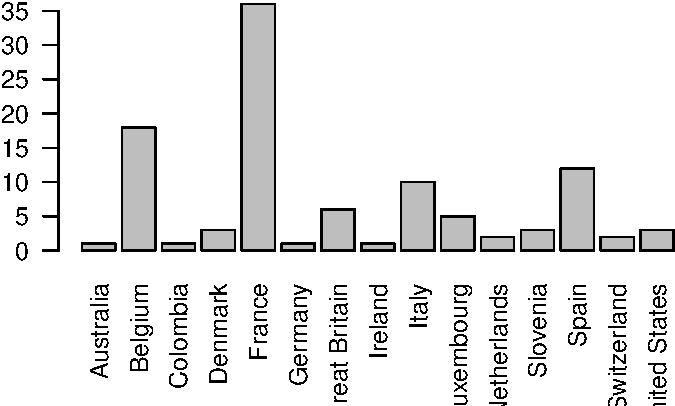
\includegraphics{022_vectors_files/figure-pdf/unnamed-chunk-17-1.pdf}

Get the victories counts in a vector can be made with \texttt{table()},
which applies to anything (numeric or character) that can be coerced to
a factor

\begin{Shaded}
\begin{Highlighting}[]
\FunctionTok{table}\NormalTok{(Winners)}
\CommentTok{\#\textgreater{} Winners}
\CommentTok{\#\textgreater{}     Australia       Belgium      Colombia       Denmark        France }
\CommentTok{\#\textgreater{}             1            18             1             3            36 }
\CommentTok{\#\textgreater{}       Germany Great Britain       Ireland         Italy    Luxembourg }
\CommentTok{\#\textgreater{}             1             6             1            10             5 }
\CommentTok{\#\textgreater{}   Netherlands      Slovenia         Spain   Switzerland United States }
\CommentTok{\#\textgreater{}             2             3            12             2             3}
\end{Highlighting}
\end{Shaded}

Both the plot and counts however follow the order of the levels, which
is alphabetical

One possibility to improve the graph is to change the order of the
levels based on the count table and redoing the graph

\begin{Shaded}
\begin{Highlighting}[]
\CommentTok{\#Vector of levels in a new order}
\NormalTok{LevelsFrq}\OtherTok{\textless{}{-}}\FunctionTok{levels}\NormalTok{(Winners)[}\FunctionTok{order}\NormalTok{(}\FunctionTok{table}\NormalTok{(Winners), }\AttributeTok{decreasing =} \ConstantTok{TRUE}\NormalTok{)]}
  \CommentTok{\#note the order function and the square brackets}
\NormalTok{LevelsFrq}
\CommentTok{\#\textgreater{}  [1] "France"        "Belgium"       "Spain"         "Italy"        }
\CommentTok{\#\textgreater{}  [5] "Great Britain" "Luxembourg"    "Denmark"       "Slovenia"     }
\CommentTok{\#\textgreater{}  [9] "United States" "Netherlands"   "Switzerland"   "Australia"    }
\CommentTok{\#\textgreater{} [13] "Colombia"      "Germany"       "Ireland"}

\CommentTok{\#Use that order when creating the factor from the character vector}
\NormalTok{WinnersFrq}\OtherTok{\textless{}{-}}\FunctionTok{factor}\NormalTok{(Winners, }\AttributeTok{levels =}\NormalTok{ LevelsFrq) }

\CommentTok{\#plot}
\FunctionTok{plot}\NormalTok{(WinnersFrq,}\AttributeTok{las=}\DecValTok{2}\NormalTok{)}
\end{Highlighting}
\end{Shaded}

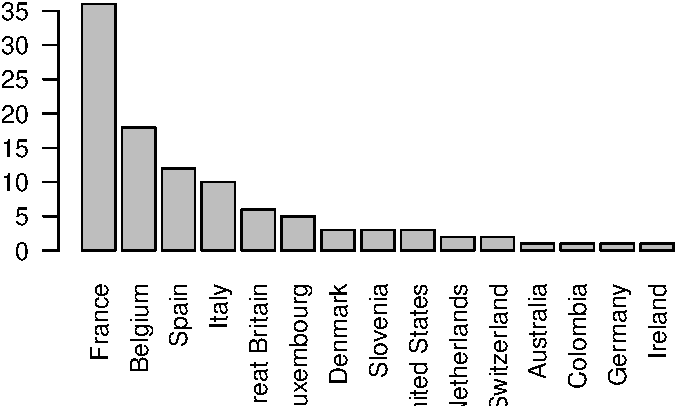
\includegraphics{022_vectors_files/figure-pdf/unnamed-chunk-19-1.pdf}

\subsection{Ordered factors}\label{ordered-factors}

Sometimes you will want to make a categorical data explicitly ordinal
for graphical or statistical purpose . For example if you have used a
Likert scale within a survey, it can be interesting it is stored as an
ordered factor. You can order an already existing factor, using the
function \texttt{ordered()}, which adds a logical flag to the factor to
indicate it is order (see first example), or at the moment you create
the factor using \texttt{factor()} (second example). Once the factor is
ordered, the levels are displayed in order and separated by a ''
\textless{} ``. Also a new class,''ordered'', is added to the object.

\begin{Shaded}
\begin{Highlighting}[]
\NormalTok{LikertScale}\OtherTok{\textless{}{-}}\FunctionTok{c}\NormalTok{(}\StringTok{"Strongly disagree"}\NormalTok{, }\StringTok{"Disagree"}\NormalTok{,}\StringTok{"Neither agree nor disagree"}\NormalTok{,}
\StringTok{"Agree"}\NormalTok{,}\StringTok{"Strongly agree"}\NormalTok{) }\CommentTok{\#in the expected order}
\NormalTok{Responses}\OtherTok{\textless{}{-}}\FunctionTok{c}\NormalTok{(}\StringTok{"Neither agree nor disagree"}\NormalTok{, }\StringTok{"Disagree"}\NormalTok{, }\StringTok{"Disagree"}\NormalTok{, }\StringTok{"Agree"}\NormalTok{, }\StringTok{"Agree"}\NormalTok{, }\StringTok{"Neither agree nor disagree"}\NormalTok{, }\StringTok{"Strongly agree"}\NormalTok{, }\StringTok{"Strongly Agree"}\NormalTok{, }\StringTok{"Disagree"}\NormalTok{)}
\NormalTok{Responses\_f}\OtherTok{\textless{}{-}}\FunctionTok{factor}\NormalTok{(Responses, }\AttributeTok{levels=}\NormalTok{LikertScale)}
\NormalTok{Responses\_f}
\CommentTok{\#\textgreater{} [1] Neither agree nor disagree Disagree                  }
\CommentTok{\#\textgreater{} [3] Disagree                   Agree                     }
\CommentTok{\#\textgreater{} [5] Agree                      Neither agree nor disagree}
\CommentTok{\#\textgreater{} [7] Strongly agree             \textless{}NA\textgreater{}                      }
\CommentTok{\#\textgreater{} [9] Disagree                  }
\CommentTok{\#\textgreater{} 5 Levels: Strongly disagree Disagree Neither agree nor disagree ... Strongly agree}

\NormalTok{Responses\_f2}\OtherTok{\textless{}{-}}\FunctionTok{ordered}\NormalTok{(Responses\_f)}
\NormalTok{Responses\_f2 }\CommentTok{\#Notice that if we don\textquotesingle{}t provide again the levels, it is made from the existing ones, so there is only 4 levels now ("Strongly Disagree" not being answered)}
\CommentTok{\#\textgreater{} [1] Neither agree nor disagree Disagree                  }
\CommentTok{\#\textgreater{} [3] Disagree                   Agree                     }
\CommentTok{\#\textgreater{} [5] Agree                      Neither agree nor disagree}
\CommentTok{\#\textgreater{} [7] Strongly agree             \textless{}NA\textgreater{}                      }
\CommentTok{\#\textgreater{} [9] Disagree                  }
\CommentTok{\#\textgreater{} Levels: Disagree \textless{} Neither agree nor disagree \textless{} Agree \textless{} Strongly agree}

\NormalTok{Responses\_f3}\OtherTok{\textless{}{-}}\FunctionTok{factor}\NormalTok{(Responses, }\AttributeTok{levels=}\NormalTok{LikertScale, }\AttributeTok{ordered =} \ConstantTok{TRUE}\NormalTok{)}
\NormalTok{Responses\_f3}
\CommentTok{\#\textgreater{} [1] Neither agree nor disagree Disagree                  }
\CommentTok{\#\textgreater{} [3] Disagree                   Agree                     }
\CommentTok{\#\textgreater{} [5] Agree                      Neither agree nor disagree}
\CommentTok{\#\textgreater{} [7] Strongly agree             \textless{}NA\textgreater{}                      }
\CommentTok{\#\textgreater{} [9] Disagree                  }
\CommentTok{\#\textgreater{} 5 Levels: Strongly disagree \textless{} Disagree \textless{} ... \textless{} Strongly agree}

\FunctionTok{class}\NormalTok{(Responses\_f3) }\CommentTok{\#see the additional class}
\CommentTok{\#\textgreater{} [1] "ordered" "factor"}
\end{Highlighting}
\end{Shaded}

In the above example you will have noticed a NA, due to some
misspelling. This is a good case to remind that categorical data should
not necessarily rely on character strings. In geography we often need to
treat countries, regions, municipalities whose names can be very
complicated, especially in multilingual context. It is good advise to
rather use codes for geographical units (e.g.~BE351, BE352, BE353, for
the NUTS 3 classification of Belgium), land use
(e.g.~\url{https://land.copernicus.eu/content/corine-land-cover-nomenclature-guidelines/html})
and relate them to a corresponding table with proper labels.

It is also true for other types of categories, including Likert scale.
An option is to use integer values (or characters for geographical
codes) together with a series of labels. You add the labels at the
moment of creating the factor:

\begin{Shaded}
\begin{Highlighting}[]
\NormalTok{LikertScale}\OtherTok{\textless{}{-}}\FunctionTok{c}\NormalTok{(}\StringTok{"Strongly disagree"}\NormalTok{, }\StringTok{"Disagree"}\NormalTok{,}\StringTok{"Neither agree nor disagree"}\NormalTok{,}
\StringTok{"Agree"}\NormalTok{,}\StringTok{"Strongly agree"}\NormalTok{) }
\NormalTok{LikertLevels}\OtherTok{\textless{}{-}}\FunctionTok{c}\NormalTok{(}\DecValTok{1}\NormalTok{L,}\DecValTok{2}\NormalTok{L,}\DecValTok{3}\NormalTok{L,}\DecValTok{4}\NormalTok{L,}\DecValTok{5}\NormalTok{L) }\CommentTok{\#would work as well with numeric c(1,2,3,4,5)}
\NormalTok{Responses}\OtherTok{\textless{}{-}}\FunctionTok{c}\NormalTok{(}\DecValTok{3}\NormalTok{L, }\DecValTok{2}\NormalTok{L, }\DecValTok{2}\NormalTok{L, }\DecValTok{4}\NormalTok{L, }\DecValTok{4}\NormalTok{L, }\DecValTok{3}\NormalTok{L, }\DecValTok{5}\NormalTok{L, }\DecValTok{5}\NormalTok{L, }\DecValTok{2}\NormalTok{L)}

\NormalTok{Responses\_f}\OtherTok{\textless{}{-}}\FunctionTok{factor}\NormalTok{(Responses, }\AttributeTok{ordered=}\ConstantTok{TRUE}\NormalTok{, }\AttributeTok{levels=}\NormalTok{LikertLevels, }\AttributeTok{labels=}\NormalTok{LikertScale)}
\NormalTok{Responses\_f}
\CommentTok{\#\textgreater{} [1] Neither agree nor disagree Disagree                  }
\CommentTok{\#\textgreater{} [3] Disagree                   Agree                     }
\CommentTok{\#\textgreater{} [5] Agree                      Neither agree nor disagree}
\CommentTok{\#\textgreater{} [7] Strongly agree             Strongly agree            }
\CommentTok{\#\textgreater{} [9] Disagree                  }
\CommentTok{\#\textgreater{} 5 Levels: Strongly disagree \textless{} Disagree \textless{} ... \textless{} Strongly agree}
\end{Highlighting}
\end{Shaded}

The result is the same as previously, but you avoid typos when inputing
the responses and can also adapt the labels at will, without changing
the data itself.

\section{Operations on vectors}\label{operations-on-vectors}

\subsection{Arithmetic operations and
recycling}\label{arithmetic-operations-and-recycling}

R is a calculator and perform the arithmetic operations \texttt{+}
\texttt{-} \texttt{*} \texttt{/} \texttt{\^{}}

Two numeric vectors of the same length can be added, multiplied, etc.
When vectors of different length are provided, the shorter one is
\emph{recycled} until the end of the longer vector. Usually a vector of
length 1 is recycled, thus allowing R to add, divide,etc. a scalar to a
vector in the same way as between two vectors (in a ``parallel way'').
But any shorter vector is also recycled (you get a warning though). See:

\begin{Shaded}
\begin{Highlighting}[]
\NormalTok{X}\OtherTok{\textless{}{-}}\FunctionTok{c}\NormalTok{(}\DecValTok{0}\NormalTok{,}\DecValTok{1}\NormalTok{,}\DecValTok{2}\NormalTok{,}\DecValTok{3}\NormalTok{,}\DecValTok{4}\NormalTok{,}\DecValTok{5}\NormalTok{)}
\NormalTok{X}\SpecialCharTok{\^{}}\DecValTok{2}
\CommentTok{\#\textgreater{} [1]  0  1  4  9 16 25}
\NormalTok{Y}\OtherTok{\textless{}{-}}\FunctionTok{c}\NormalTok{(}\DecValTok{10}\NormalTok{,}\DecValTok{9}\NormalTok{,}\DecValTok{8}\NormalTok{,}\DecValTok{7}\NormalTok{,}\DecValTok{6}\NormalTok{,}\DecValTok{5}\NormalTok{)}

\NormalTok{X}\SpecialCharTok{+}\NormalTok{Y}
\CommentTok{\#\textgreater{} [1] 10 10 10 10 10 10}
\NormalTok{Y}\SpecialCharTok{/}\NormalTok{X}
\CommentTok{\#\textgreater{} [1]      Inf 9.000000 4.000000 2.333333 1.500000 1.000000}
\NormalTok{X}\SpecialCharTok{*}\FunctionTok{c}\NormalTok{(}\DecValTok{0}\NormalTok{,}\DecValTok{1}\NormalTok{)}
\CommentTok{\#\textgreater{} [1] 0 1 0 3 0 5}
\end{Highlighting}
\end{Shaded}

You can also apply a series of common mathematical functions to any
numeric vector.

\begin{Shaded}
\begin{Highlighting}[]
\NormalTok{a}\OtherTok{\textless{}{-}}\FunctionTok{c}\NormalTok{(}\SpecialCharTok{{-}}\DecValTok{2}\NormalTok{,}\SpecialCharTok{{-}}\DecValTok{1}\NormalTok{,}\DecValTok{0}\NormalTok{,}\DecValTok{1}\NormalTok{,}\DecValTok{2}\NormalTok{,}\DecValTok{6}\NormalTok{,}\DecValTok{10}\NormalTok{)}
\FunctionTok{abs}\NormalTok{(a) }\CommentTok{\#absolute}
\CommentTok{\#\textgreater{} [1]  2  1  0  1  2  6 10}

\NormalTok{a}\SpecialCharTok{\^{}}\NormalTok{(}\SpecialCharTok{{-}}\DecValTok{1}\NormalTok{) }\CommentTok{\#inverse}
\CommentTok{\#\textgreater{} [1] {-}0.5000000 {-}1.0000000        Inf  1.0000000  0.5000000  0.1666667  0.1000000}

\FunctionTok{log}\NormalTok{(a) }\CommentTok{\#ln or Natural logarithm (or Napierian logarithm)}
\CommentTok{\#\textgreater{} Warning in log(a): NaNs produced}
\CommentTok{\#\textgreater{} [1]       NaN       NaN      {-}Inf 0.0000000 0.6931472 1.7917595 2.3025851}
\FunctionTok{log10}\NormalTok{(a) }\CommentTok{\# base 10 logarithm}
\CommentTok{\#\textgreater{} Warning: NaNs produced}
\CommentTok{\#\textgreater{} [1]       NaN       NaN      {-}Inf 0.0000000 0.3010300 0.7781513 1.0000000}

\FunctionTok{exp}\NormalTok{(a) }\CommentTok{\#base e exponential}
\CommentTok{\#\textgreater{} [1] 1.353353e{-}01 3.678794e{-}01 1.000000e+00 2.718282e+00 7.389056e+00}
\CommentTok{\#\textgreater{} [6] 4.034288e+02 2.202647e+04}
\DecValTok{10}\SpecialCharTok{\^{}}\NormalTok{a }\CommentTok{\#base 10 exponential}
\CommentTok{\#\textgreater{} [1] 1e{-}02 1e{-}01 1e+00 1e+01 1e+02 1e+06 1e+10}

\FunctionTok{sqrt}\NormalTok{(a) }\CommentTok{\#square root}
\CommentTok{\#\textgreater{} Warning in sqrt(a): NaNs produced}
\CommentTok{\#\textgreater{} [1]      NaN      NaN 0.000000 1.000000 1.414214 2.449490 3.162278}
\end{Highlighting}
\end{Shaded}

See Crawley (2012) p.11 for more examples:

\begin{figure}[H]

{\centering 
\includegraphics{images/mathFunctionsR.png}

}

\caption{Crawley Table 2.1}

\end{figure}%

Be careful that these functions must lead to proper results. As you can
see from the warnings. ``NaN'' stands for ``Not a Number'' and is
considered as NA (``not available''). Which is not the case of infinity,
which is a numeric

\begin{Shaded}
\begin{Highlighting}[]
\NormalTok{a}\OtherTok{\textless{}{-}}\FunctionTok{c}\NormalTok{(}\SpecialCharTok{{-}}\DecValTok{2}\NormalTok{,}\SpecialCharTok{{-}}\DecValTok{1}\NormalTok{,}\DecValTok{0}\NormalTok{,}\DecValTok{1}\NormalTok{,}\DecValTok{2}\NormalTok{,}\DecValTok{6}\NormalTok{,}\DecValTok{10}\NormalTok{)}
\FunctionTok{is.na}\NormalTok{(}\ConstantTok{NaN}\NormalTok{)}
\CommentTok{\#\textgreater{} [1] TRUE}
\FunctionTok{is.na}\NormalTok{(}\SpecialCharTok{{-}}\ConstantTok{Inf}\NormalTok{)}
\CommentTok{\#\textgreater{} [1] FALSE}
\FunctionTok{is.finite}\NormalTok{(}\FunctionTok{log10}\NormalTok{(a))}
\CommentTok{\#\textgreater{} Warning: NaNs produced}
\CommentTok{\#\textgreater{} [1] FALSE FALSE FALSE  TRUE  TRUE  TRUE  TRUE}
\end{Highlighting}
\end{Shaded}

\subsection{Euclidean division and
rounding}\label{euclidean-division-and-rounding}

The modulo operation for integers is obtained with \texttt{\%/\%} to get
the integral part of the Euclidean division and \texttt{\%\%} to get the
remainder. This the way you will know an integer is odd or even. The
function can also be applied to numeric vectors with decimals.

\begin{Shaded}
\begin{Highlighting}[]
\FunctionTok{c}\NormalTok{(}\DecValTok{1}\NormalTok{,}\DecValTok{3}\NormalTok{,}\DecValTok{5}\NormalTok{,}\DecValTok{44}\NormalTok{,}\DecValTok{444}\NormalTok{,}\DecValTok{4444}\NormalTok{)}\SpecialCharTok{\%/\%}\DecValTok{2}
\CommentTok{\#\textgreater{} [1]    0    1    2   22  222 2222}
\FunctionTok{c}\NormalTok{(}\DecValTok{1}\NormalTok{,}\DecValTok{3}\NormalTok{,}\DecValTok{5}\NormalTok{,}\DecValTok{44}\NormalTok{,}\DecValTok{444}\NormalTok{,}\DecValTok{4444}\NormalTok{)}\SpecialCharTok{\%\%}\DecValTok{2} \CommentTok{\#remainder of dividing by 2, thus indicating odd/even}
\CommentTok{\#\textgreater{} [1] 1 1 1 0 0 0}
\FloatTok{99.99}\SpecialCharTok{\%/\%}\DecValTok{2}
\CommentTok{\#\textgreater{} [1] 49}
\FloatTok{99.99}\SpecialCharTok{\%\%}\DecValTok{2}
\CommentTok{\#\textgreater{} [1] 1.99}
\end{Highlighting}
\end{Shaded}

For ratio and interval numbers with decimals you sometimes need to get
rid of the decimals or display only a part of them Examine the
following:

\begin{Shaded}
\begin{Highlighting}[]
\NormalTok{x}\OtherTok{\textless{}{-}}\FunctionTok{c}\NormalTok{(}\FloatTok{33.33}\NormalTok{, }\FloatTok{666.166}\NormalTok{, }\FloatTok{50.5}\NormalTok{, }\FloatTok{49.5}\NormalTok{)}
\FunctionTok{trunc}\NormalTok{(x) }\CommentTok{\#compares with as.integer() but does not change the class to integer}
\CommentTok{\#\textgreater{} [1]  33 666  50  49}
\FunctionTok{round}\NormalTok{(x) }\CommentTok{\#note the rounding of a 5 to the even digit (international standard) }
\CommentTok{\#\textgreater{} [1]  33 666  50  50}
\FunctionTok{round}\NormalTok{(x, }\AttributeTok{digits=}\DecValTok{2}\NormalTok{)}
\CommentTok{\#\textgreater{} [1]  33.33 666.17  50.50  49.50}
\FunctionTok{ceiling}\NormalTok{(x)}
\CommentTok{\#\textgreater{} [1]  34 667  51  50}
\FunctionTok{floor}\NormalTok{(x)}
\CommentTok{\#\textgreater{} [1]  33 666  50  49}

\FunctionTok{signif}\NormalTok{(x, }\AttributeTok{digits =} \DecValTok{5}\NormalTok{)}
\CommentTok{\#\textgreater{} [1]  33.33 666.17  50.50  49.50}
\end{Highlighting}
\end{Shaded}

With geographical data, \texttt{ceiling()} can for example be applied to
latitudes and longitudes in order to make grids. A simple example is how
to obtain (theoretical) time zones from a set of longitudes.

Let's take the opportunity to learn about \texttt{set.seed()} and about
uniform random number generation \texttt{runif()}:

\begin{Shaded}
\begin{Highlighting}[]
\FunctionTok{set.seed}\NormalTok{(}\DecValTok{101}\NormalTok{)}
\NormalTok{Longitudes}\OtherTok{\textless{}{-}}\FunctionTok{runif}\NormalTok{(}\AttributeTok{n=}\DecValTok{10}\NormalTok{,}\AttributeTok{min=}\SpecialCharTok{{-}}\DecValTok{180}\NormalTok{, }\AttributeTok{max=}\DecValTok{180}\NormalTok{)}
\NormalTok{Longitudes}
\CommentTok{\#\textgreater{}  [1]  {-}46.00858 {-}164.22307   75.48625   56.76854  {-}90.05194  {-}71.98026}
\CommentTok{\#\textgreater{}  [7]   30.55199  {-}59.95183   43.92431   16.49828}

\FunctionTok{ceiling}\NormalTok{(Longitudes}\SpecialCharTok{*}\DecValTok{24}\SpecialCharTok{/}\DecValTok{360}\NormalTok{)}
\CommentTok{\#\textgreater{}  [1]  {-}3 {-}10   6   4  {-}6  {-}4   3  {-}3   3   2}
\end{Highlighting}
\end{Shaded}

\begin{figure}[H]

{\centering 
\includegraphics{images/clipboard-2750177594.png}

}

\caption{\href{https://en.wikipedia.org/wiki/Time_zone\#/media/File:World_Time_Zone_Chart_1942.jpg}{Wikipedia,
Time Zones}}

\end{figure}%

\subsection{Logical and Boolean
operations}\label{logical-and-boolean-operations}

A series of operations return a \textbf{logical vector}, i.e.~a vector
of Boolean values \textbf{TRUE and FALSE}.

Those operations are \texttt{\textgreater{}}, \texttt{\textgreater{}=},
\texttt{\textless{}}, \texttt{\textless{}=}, \texttt{==}, \texttt{!=}

Some examples with numeric and character vectors:

\textbf{IMPORTANT: Use \texttt{==} for comparison, not \texttt{=}, which
is an assignment!}

\begin{Shaded}
\begin{Highlighting}[]
\FunctionTok{c}\NormalTok{(}\DecValTok{1}\NormalTok{,}\DecValTok{2}\NormalTok{,}\DecValTok{3}\NormalTok{) }\SpecialCharTok{\textless{}} \FunctionTok{c}\NormalTok{(}\DecValTok{2}\NormalTok{,}\DecValTok{3}\NormalTok{,}\DecValTok{3}\NormalTok{)}
\CommentTok{\#\textgreater{} [1]  TRUE  TRUE FALSE}
\FunctionTok{c}\NormalTok{(}\DecValTok{1}\NormalTok{,}\DecValTok{2}\NormalTok{,}\DecValTok{3}\NormalTok{) }\SpecialCharTok{\textgreater{}=} \DecValTok{3} \CommentTok{\#see right hand side is recycled and applied "one to one"}
\CommentTok{\#\textgreater{} [1] FALSE FALSE  TRUE}
\StringTok{"Bernadette, elle est très chouette"} \SpecialCharTok{==} \StringTok{"Bernadette, elle est très chouette"}
\CommentTok{\#\textgreater{} [1] TRUE}
\StringTok{"Bernadette, elle est très chouette"} \SpecialCharTok{!=} \StringTok{"Mais sa cousine, elle est divine"}
\CommentTok{\#\textgreater{} [1] TRUE}
\StringTok{"Julian"} \SpecialCharTok{\textgreater{}=} \StringTok{"Julien"} \CommentTok{\#alphabetical order}
\CommentTok{\#\textgreater{} [1] FALSE}
\end{Highlighting}
\end{Shaded}

By the way we see here vectors of the \textbf{logical class}:

\begin{Shaded}
\begin{Highlighting}[]
\FunctionTok{class}\NormalTok{(}\StringTok{"Julian"} \SpecialCharTok{\textgreater{}=} \StringTok{"Julien"}\NormalTok{)}
\CommentTok{\#\textgreater{} [1] "logical"}
\end{Highlighting}
\end{Shaded}

In addition to those comparisons, many functions, especially structured
as ``is.xxx'' return a TRUE or FALSE and are very useful within you data
management process. You may make quite some use also of the \%in\%
function, when you have a long vector, to check whether a particular
value (or several) is present within a vector.

\begin{Shaded}
\begin{Highlighting}[]
\FunctionTok{is.numeric}\NormalTok{(}\StringTok{"a"}\NormalTok{)}
\CommentTok{\#\textgreater{} [1] FALSE}
\FunctionTok{is.numeric}\NormalTok{(}\StringTok{"2"}\NormalTok{)}
\CommentTok{\#\textgreater{} [1] FALSE}
\FunctionTok{is.numeric}\NormalTok{(}\DecValTok{3}\NormalTok{L)}
\CommentTok{\#\textgreater{} [1] TRUE}
\FunctionTok{is.numeric}\NormalTok{(}\ConstantTok{FALSE}\NormalTok{)}
\CommentTok{\#\textgreater{} [1] FALSE}
\SpecialCharTok{!}\FunctionTok{is.numeric}\NormalTok{(}\ConstantTok{FALSE}\NormalTok{) }\CommentTok{\#Note the negation here!}
\CommentTok{\#\textgreater{} [1] TRUE}

\StringTok{"urban"} \SpecialCharTok{\%in\%} \FunctionTok{c}\NormalTok{(}\StringTok{"urban"}\NormalTok{,}\StringTok{"agriculture"}\NormalTok{,}\StringTok{"water"}\NormalTok{,}\StringTok{"forest"}\NormalTok{)}
\CommentTok{\#\textgreater{} [1] TRUE}
\FunctionTok{c}\NormalTok{(}\StringTok{"urban"}\NormalTok{,}\StringTok{"industry"}\NormalTok{) }\SpecialCharTok{\%in\%} \FunctionTok{c}\NormalTok{(}\StringTok{"urban"}\NormalTok{,}\StringTok{"agriculture"}\NormalTok{,}\StringTok{"water"}\NormalTok{,}\StringTok{"forest"}\NormalTok{)}
\CommentTok{\#\textgreater{} [1]  TRUE FALSE}
\end{Highlighting}
\end{Shaded}

Boolean values are usually (always?) coerced to a \textbf{1 and 0}, in
case an arithmetic operation is then demanded.

\begin{Shaded}
\begin{Highlighting}[]
\FunctionTok{mean}\NormalTok{(}\FunctionTok{c}\NormalTok{(}\ConstantTok{TRUE}\NormalTok{,}\ConstantTok{FALSE}\NormalTok{,}\ConstantTok{TRUE}\NormalTok{,}\ConstantTok{TRUE}\NormalTok{))}
\CommentTok{\#\textgreater{} [1] 0.75}
\FunctionTok{sum}\NormalTok{(}\FunctionTok{c}\NormalTok{(}\ConstantTok{TRUE}\NormalTok{,}\ConstantTok{FALSE}\NormalTok{,}\ConstantTok{TRUE}\NormalTok{,}\ConstantTok{TRUE}\NormalTok{))}
\CommentTok{\#\textgreater{} [1] 3}
\DecValTok{3}\SpecialCharTok{*}\NormalTok{(}\FunctionTok{c}\NormalTok{(}\ConstantTok{TRUE}\NormalTok{,}\ConstantTok{FALSE}\NormalTok{)}\SpecialCharTok{+}\ConstantTok{TRUE}\NormalTok{)}
\CommentTok{\#\textgreater{} [1] 6 3}
\end{Highlighting}
\end{Shaded}

A set of functions then apply specifically to the Boolean values TRUE or
FALSE, i.e.~to logical vectors.

These logical operators are: \texttt{!}, \texttt{\&},
\texttt{\textbar{}}, \texttt{xor} and typically used to \textbf{select
elements that match 2 or more conditions}.

The graphic below, reproduced from \href{https://r4ds.hadley.nz/}{R for
Data Science} (highly recommended!), demonstrate their outcome for 2
sets and an example is provided after creating 2 logical vectors, x and
y from the LETTERS character vector.

\begin{figure}[H]

{\centering 
\includegraphics{images/clipboard-4033778274.png}

}

\caption{source: Fig.12.1 from https://r4ds.hadley.nz/logicals}

\end{figure}%

\begin{Shaded}
\begin{Highlighting}[]
\NormalTok{LETTERS[}\DecValTok{1}\SpecialCharTok{:}\DecValTok{6}\NormalTok{]}
\CommentTok{\#\textgreater{} [1] "A" "B" "C" "D" "E" "F"}
\NormalTok{x}\OtherTok{\textless{}{-}}\NormalTok{LETTERS[}\DecValTok{1}\SpecialCharTok{:}\DecValTok{6}\NormalTok{]}\SpecialCharTok{\textless{}}\StringTok{"E"}
\NormalTok{y}\OtherTok{\textless{}{-}}\NormalTok{LETTERS[}\DecValTok{1}\SpecialCharTok{:}\DecValTok{6}\NormalTok{]}\SpecialCharTok{\textgreater{}}\StringTok{"B"}
\NormalTok{x}
\CommentTok{\#\textgreater{} [1]  TRUE  TRUE  TRUE  TRUE FALSE FALSE}
\NormalTok{y}
\CommentTok{\#\textgreater{} [1] FALSE FALSE  TRUE  TRUE  TRUE  TRUE}
\NormalTok{x }\SpecialCharTok{\&}\NormalTok{ y}
\CommentTok{\#\textgreater{} [1] FALSE FALSE  TRUE  TRUE FALSE FALSE}
\NormalTok{x }\SpecialCharTok{\&} \SpecialCharTok{!}\NormalTok{y}
\CommentTok{\#\textgreater{} [1]  TRUE  TRUE FALSE FALSE FALSE FALSE}
\SpecialCharTok{!}\NormalTok{x }\SpecialCharTok{\&}\NormalTok{ y}
\CommentTok{\#\textgreater{} [1] FALSE FALSE FALSE FALSE  TRUE  TRUE}
\NormalTok{x }\SpecialCharTok{\&}\NormalTok{ y}
\CommentTok{\#\textgreater{} [1] FALSE FALSE  TRUE  TRUE FALSE FALSE}
\NormalTok{x }\SpecialCharTok{|}\NormalTok{ y}
\CommentTok{\#\textgreater{} [1] TRUE TRUE TRUE TRUE TRUE TRUE}
\FunctionTok{xor}\NormalTok{(x,y)}
\CommentTok{\#\textgreater{} [1]  TRUE  TRUE FALSE FALSE  TRUE  TRUE}
\end{Highlighting}
\end{Shaded}

\section{Vectors' functions}\label{vectors-functions}

A number of functions are evaluated over an entire vector (vectorisation
is there to avoid loops) and used to describe and understand the
distribution of values. They apply mostly to numeric vectors but also to
logicals (being 0 or 1 anyway) as well as characters, where possible
(based on alphabetical order).

\subsection{Range, cumulative values, positions and
sorting}\label{range-cumulative-values-positions-and-sorting}

\begin{longtable}[]{@{}llll@{}}
\caption{Examples of functions evaluated over an entire
vector}\tabularnewline
\toprule\noalign{}
\endfirsthead
\endhead
\bottomrule\noalign{}
\endlastfoot
\texttt{min(x)} & \texttt{cummin(x)} & \texttt{which.min(x)} &
\texttt{sort(x)} \\
\texttt{max(x)} & \texttt{cummax(x)} & \texttt{which.max(x)} &
\texttt{order(x)} \\
\texttt{range(x)} & & & \texttt{rank(x)} \\
\texttt{sum(x)} & \texttt{cumsum(x)} & & \\
\end{longtable}

Let's explore some of those for x being a numeric, a logical and
character. \emph{In class exploration.}

It is sometimes difficult to remember differences between
\texttt{sort(x)},\texttt{order(x)} and \texttt{rank(x)}

See two examples below

\begin{Shaded}
\begin{Highlighting}[]
\FunctionTok{set.seed}\NormalTok{(}\DecValTok{101}\NormalTok{)}
\NormalTok{x}\OtherTok{\textless{}{-}}\FunctionTok{round}\NormalTok{(}\FunctionTok{runif}\NormalTok{(}\DecValTok{10}\NormalTok{,}\DecValTok{100}\NormalTok{,}\DecValTok{200}\NormalTok{))}
\NormalTok{x}
\CommentTok{\#\textgreater{}  [1] 137 104 171 166 125 130 158 133 162 155}

\FunctionTok{cbind}\NormalTok{(}\AttributeTok{Original=}\NormalTok{x,}\AttributeTok{Sorted=}\FunctionTok{sort}\NormalTok{(x),}\AttributeTok{Rank=}\FunctionTok{rank}\NormalTok{(x),}\AttributeTok{Order=}\FunctionTok{order}\NormalTok{(x))}
\CommentTok{\#\textgreater{}       Original Sorted Rank Order}
\CommentTok{\#\textgreater{}  [1,]      137    104    5     2}
\CommentTok{\#\textgreater{}  [2,]      104    125    1     5}
\CommentTok{\#\textgreater{}  [3,]      171    130   10     6}
\CommentTok{\#\textgreater{}  [4,]      166    133    9     8}
\CommentTok{\#\textgreater{}  [5,]      125    137    2     1}
\CommentTok{\#\textgreater{}  [6,]      130    155    3    10}
\CommentTok{\#\textgreater{}  [7,]      158    158    7     7}
\CommentTok{\#\textgreater{}  [8,]      133    162    4     9}
\CommentTok{\#\textgreater{}  [9,]      162    166    8     4}
\CommentTok{\#\textgreater{} [10,]      155    171    6     3}
\end{Highlighting}
\end{Shaded}

\begin{Shaded}
\begin{Highlighting}[]
\NormalTok{M}\OtherTok{\textless{}{-}}\NormalTok{month.name[}\DecValTok{1}\SpecialCharTok{:}\DecValTok{6}\NormalTok{]}
\NormalTok{M}
\CommentTok{\#\textgreater{} [1] "January"  "February" "March"    "April"    "May"      "June"}

\FunctionTok{cbind}\NormalTok{(}\AttributeTok{Months=}\NormalTok{M,}\AttributeTok{Sorted=}\FunctionTok{sort}\NormalTok{(M),}\AttributeTok{Rank=}\FunctionTok{rank}\NormalTok{(M),}\AttributeTok{Order=}\FunctionTok{order}\NormalTok{(M))}
\CommentTok{\#\textgreater{}      Months     Sorted     Rank Order}
\CommentTok{\#\textgreater{} [1,] "January"  "April"    "3"  "4"  }
\CommentTok{\#\textgreater{} [2,] "February" "February" "2"  "2"  }
\CommentTok{\#\textgreater{} [3,] "March"    "January"  "5"  "1"  }
\CommentTok{\#\textgreater{} [4,] "April"    "June"     "1"  "6"  }
\CommentTok{\#\textgreater{} [5,] "May"      "March"    "6"  "3"  }
\CommentTok{\#\textgreater{} [6,] "June"     "May"      "4"  "5"}
\end{Highlighting}
\end{Shaded}

To those operations, we should add all univariate statistics such as
\texttt{mean()}, \texttt{median()}, \texttt{var()}, \texttt{quantile()},
but we leave them aside for now as they are introduced later with
univariate statistics and distributions.

Specific to logical vectors, the \texttt{any()} and \texttt{all()}
functions are particularly useful in the case you check a very long
vector with only very few having a TRUE or a FALSE.

See basic examples:

\begin{Shaded}
\begin{Highlighting}[]
\FunctionTok{any}\NormalTok{(}\FunctionTok{c}\NormalTok{(}\ConstantTok{TRUE}\NormalTok{,}\ConstantTok{TRUE}\NormalTok{,}\ConstantTok{TRUE}\NormalTok{,}\ConstantTok{FALSE}\NormalTok{))}
\CommentTok{\#\textgreater{} [1] TRUE}
\FunctionTok{any}\NormalTok{(}\FunctionTok{c}\NormalTok{(}\ConstantTok{TRUE}\NormalTok{,}\ConstantTok{TRUE}\NormalTok{,}\ConstantTok{TRUE}\NormalTok{,}\ConstantTok{TRUE}\NormalTok{))}
\CommentTok{\#\textgreater{} [1] TRUE}
\FunctionTok{all}\NormalTok{(}\FunctionTok{c}\NormalTok{(}\ConstantTok{TRUE}\NormalTok{,}\ConstantTok{TRUE}\NormalTok{,}\ConstantTok{TRUE}\NormalTok{,}\ConstantTok{FALSE}\NormalTok{))}
\CommentTok{\#\textgreater{} [1] FALSE}
\end{Highlighting}
\end{Shaded}

And an example where we suppose a random set of values from a normal
distribution and we want to check manually whether there is an upper
outlier. Typically (as in boxplots) this outlier is calculated as being
any value above the 3rd quartile plus 1.5 times the interquartile range.

\begin{Shaded}
\begin{Highlighting}[]
\FunctionTok{set.seed}\NormalTok{(}\DecValTok{102}\NormalTok{)}
\NormalTok{x}\OtherTok{\textless{}{-}}\FunctionTok{rnorm}\NormalTok{(}\DecValTok{100}\NormalTok{)}
\NormalTok{q75}\OtherTok{\textless{}{-}}\FunctionTok{quantile}\NormalTok{(x, }\AttributeTok{p=}\FloatTok{0.75}\NormalTok{)}
\NormalTok{iqr}\OtherTok{\textless{}{-}}\FunctionTok{IQR}\NormalTok{(x)}
\FunctionTok{any}\NormalTok{(x}\SpecialCharTok{\textgreater{}}\NormalTok{(q75}\FloatTok{+1.5}\SpecialCharTok{*}\NormalTok{iqr))}
\CommentTok{\#\textgreater{} [1] TRUE}
\FunctionTok{boxplot}\NormalTok{(x) }\CommentTok{\#}
\end{Highlighting}
\end{Shaded}

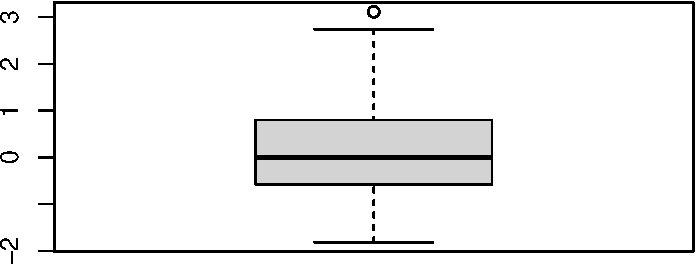
\includegraphics{022_vectors_files/figure-pdf/unnamed-chunk-36-1.pdf}

\begin{Shaded}
\begin{Highlighting}[]
\NormalTok{x[x}\SpecialCharTok{\textgreater{}}\NormalTok{(q75}\FloatTok{+1.5}\SpecialCharTok{*}\NormalTok{iqr)] }\CommentTok{\#to identify them}
\CommentTok{\#\textgreater{} [1] 3.114333}

\FunctionTok{set.seed}\NormalTok{(}\DecValTok{101}\NormalTok{) }\CommentTok{\#Check with this seed!}
\end{Highlighting}
\end{Shaded}

\subsection{Summary}\label{summary}

One of the most used function for analysis (if not THE most used) is
\texttt{summary()}. We will see its result may change substantially
based on the object class it is applied to. Its basic functioning for a
simple numeric vector and character vector is:

\begin{Shaded}
\begin{Highlighting}[]
\FunctionTok{summary}\NormalTok{(}\FunctionTok{c}\NormalTok{(}\DecValTok{1}\NormalTok{,}\DecValTok{2}\NormalTok{,}\DecValTok{3}\NormalTok{,}\DecValTok{4}\NormalTok{,}\ConstantTok{NA}\NormalTok{,}\DecValTok{6}\NormalTok{))}
\CommentTok{\#\textgreater{}    Min. 1st Qu.  Median    Mean 3rd Qu.    Max.    NA\textquotesingle{}s }
\CommentTok{\#\textgreater{}     1.0     2.0     3.0     3.2     4.0     6.0       1}
\FunctionTok{summary}\NormalTok{(}\FunctionTok{c}\NormalTok{(}\StringTok{"A"}\NormalTok{,}\StringTok{"B"}\NormalTok{,}\StringTok{"C"}\NormalTok{,}\ConstantTok{NA}\NormalTok{,}\ConstantTok{NA}\NormalTok{,}\StringTok{"F"}\NormalTok{))}
\CommentTok{\#\textgreater{}    Length     Class      Mode }
\CommentTok{\#\textgreater{}         6 character character}
\end{Highlighting}
\end{Shaded}

\subsection{Element-wise functions}\label{element-wise-functions}

Other functions apply to two or more vectors. They need an x and a y
vector as input, e.g.~\texttt{cor(x,y)}. Most of those you will
encounter use two vectors of the same length and type, i.e.~no
recycling, which leads us to the notion of a data frame (see next
chapter).

At this time, we show only two simple ``parallel'' or ``element-wise''
computations: \texttt{pmin()} and \texttt{pmax()}, which can be useful
for example when there is a repeated measure for a given set of
individuals. Cases are not rare when you make a new vector (or column in
a data frame) based on such element-wise calculations. (Yet you would
probably assemble the data into a data frame first and then make a
row-wise calculation).

\begin{Shaded}
\begin{Highlighting}[]
\NormalTok{t1}\OtherTok{\textless{}{-}}\FunctionTok{c}\NormalTok{(}\DecValTok{25}\NormalTok{,}\DecValTok{35}\NormalTok{,}\DecValTok{45}\NormalTok{,}\DecValTok{55}\NormalTok{)}
\NormalTok{t2}\OtherTok{\textless{}{-}}\FunctionTok{c}\NormalTok{(}\DecValTok{26}\NormalTok{,}\DecValTok{36}\NormalTok{,}\DecValTok{44}\NormalTok{,}\DecValTok{54}\NormalTok{)}
\NormalTok{t3}\OtherTok{\textless{}{-}}\FunctionTok{c}\NormalTok{(}\DecValTok{27}\NormalTok{,}\DecValTok{34}\NormalTok{,}\DecValTok{43}\NormalTok{,}\DecValTok{56}\NormalTok{)}

\FunctionTok{pmin}\NormalTok{(t1,t2,t3)}
\CommentTok{\#\textgreater{} [1] 25 34 43 54}
\FunctionTok{pmax}\NormalTok{(t1,t2,t3)}
\CommentTok{\#\textgreater{} [1] 27 36 45 56}
\end{Highlighting}
\end{Shaded}

\section{Indexing and subsetting}\label{indexing-and-subsetting}

Now you have seen that vectors are the key elements in R, you will still
want to access its elements individually or parts of it based on
positions or conditions

Square brackets I used to get into vector elements by their position (or
by their name if named).

You can supply one position but also several positions and ranges.
Examine the following:

\begin{Shaded}
\begin{Highlighting}[]
\NormalTok{x}\OtherTok{\textless{}{-}}\FunctionTok{c}\NormalTok{(}\DecValTok{3}\NormalTok{,}\DecValTok{1}\NormalTok{,}\DecValTok{9}\NormalTok{,}\DecValTok{7}\NormalTok{,}\DecValTok{8}\NormalTok{,}\DecValTok{2}\NormalTok{,}\DecValTok{3}\NormalTok{,}\DecValTok{6}\NormalTok{,}\DecValTok{3}\NormalTok{,}\DecValTok{4}\NormalTok{)}
\NormalTok{x }\CommentTok{\#all}
\CommentTok{\#\textgreater{}  [1] 3 1 9 7 8 2 3 6 3 4}
\NormalTok{x[}\DecValTok{4}\NormalTok{] }\CommentTok{\#4th element}
\CommentTok{\#\textgreater{} [1] 7}
\NormalTok{x[}\DecValTok{6}\SpecialCharTok{:}\DecValTok{8}\NormalTok{] }\CommentTok{\#a sequence}
\CommentTok{\#\textgreater{} [1] 2 3 6}
\NormalTok{x[}\FunctionTok{c}\NormalTok{(}\DecValTok{4}\NormalTok{,}\DecValTok{6}\SpecialCharTok{:}\DecValTok{8}\NormalTok{)] }\CommentTok{\#both}
\CommentTok{\#\textgreater{} [1] 7 2 3 6}
\NormalTok{x[}\SpecialCharTok{{-}}\DecValTok{4}\NormalTok{] }\CommentTok{\#all but the 4th element}
\CommentTok{\#\textgreater{} [1] 3 1 9 8 2 3 6 3 4}
\NormalTok{x[}\SpecialCharTok{{-}}\FunctionTok{length}\NormalTok{(x)] }\CommentTok{\#all but the last one}
\CommentTok{\#\textgreater{} [1] 3 1 9 7 8 2 3 6 3}
\NormalTok{x[}\SpecialCharTok{{-}}\NormalTok{((}\FunctionTok{length}\NormalTok{(x)}\SpecialCharTok{{-}}\DecValTok{1}\NormalTok{)}\SpecialCharTok{:}\FunctionTok{length}\NormalTok{(x))]  }\CommentTok{\#all but the last two}
\CommentTok{\#\textgreater{} [1] 3 1 9 7 8 2 3 6}
\end{Highlighting}
\end{Shaded}

This is very flexible because you can use any vector representing an
index (position) to make a new vector.

\begin{Shaded}
\begin{Highlighting}[]
\NormalTok{x}\OtherTok{\textless{}{-}}\FunctionTok{c}\NormalTok{(}\DecValTok{3}\NormalTok{,}\DecValTok{1}\NormalTok{,}\DecValTok{9}\NormalTok{,}\DecValTok{7}\NormalTok{,}\DecValTok{8}\NormalTok{,}\DecValTok{2}\NormalTok{,}\DecValTok{3}\NormalTok{,}\DecValTok{6}\NormalTok{,}\DecValTok{3}\NormalTok{,}\DecValTok{4}\NormalTok{)}
\NormalTok{chicken}\OtherTok{\textless{}{-}}\FunctionTok{c}\NormalTok{(}\DecValTok{10}\NormalTok{,}\DecValTok{10}\NormalTok{,}\DecValTok{10}\NormalTok{,}\DecValTok{4}\NormalTok{,}\DecValTok{2}\NormalTok{,}\DecValTok{3}\NormalTok{)}
\NormalTok{x[chicken]}
\CommentTok{\#\textgreater{} [1] 4 4 4 7 1 9}
\end{Highlighting}
\end{Shaded}

Such a vector can be a logical, then the elements where the logical is
TRUE are returned.

\begin{Shaded}
\begin{Highlighting}[]
\NormalTok{x}\OtherTok{\textless{}{-}}\FunctionTok{c}\NormalTok{(}\DecValTok{3}\NormalTok{,}\DecValTok{1}\NormalTok{,}\DecValTok{9}\NormalTok{,}\DecValTok{7}\NormalTok{,}\DecValTok{8}\NormalTok{,}\DecValTok{2}\NormalTok{,}\DecValTok{3}\NormalTok{,}\DecValTok{6}\NormalTok{,}\DecValTok{3}\NormalTok{,}\DecValTok{4}\NormalTok{)}
\NormalTok{x}\SpecialCharTok{\textgreater{}}\DecValTok{3}
\CommentTok{\#\textgreater{}  [1] FALSE FALSE  TRUE  TRUE  TRUE FALSE FALSE  TRUE FALSE  TRUE}
\NormalTok{x[x}\SpecialCharTok{\textgreater{}}\DecValTok{3}\NormalTok{]}
\CommentTok{\#\textgreater{} [1] 9 7 8 6 4}

\NormalTok{x }\SpecialCharTok{\%\%} \DecValTok{2} \SpecialCharTok{==} \DecValTok{0}
\CommentTok{\#\textgreater{}  [1] FALSE FALSE FALSE FALSE  TRUE  TRUE FALSE  TRUE FALSE  TRUE}
\NormalTok{x[x }\SpecialCharTok{\%\%} \DecValTok{2} \SpecialCharTok{==} \DecValTok{0}\NormalTok{] }\CommentTok{\#even numbers only}
\CommentTok{\#\textgreater{} [1] 8 2 6 4}

\NormalTok{x[x}\SpecialCharTok{\textgreater{}}\FunctionTok{mean}\NormalTok{(x)]}
\CommentTok{\#\textgreater{} [1] 9 7 8 6}

\NormalTok{x[}\FunctionTok{as.logical}\NormalTok{(}\FunctionTok{c}\NormalTok{(}\DecValTok{0}\NormalTok{,}\DecValTok{1}\NormalTok{))] }\CommentTok{\#?? recyling is in effect here}
\CommentTok{\#\textgreater{} [1] 1 7 2 6 4}
\end{Highlighting}
\end{Shaded}

Possibilities are endless, especially if you think the indexing vector
can come from another vector than x.

Vectors are sometimes named, and names the used to retrieve the data:

\begin{Shaded}
\begin{Highlighting}[]
\NormalTok{y}\OtherTok{\textless{}{-}}\FunctionTok{c}\NormalTok{(}\DecValTok{1000}\NormalTok{,}\DecValTok{1500}\NormalTok{,}\DecValTok{900}\NormalTok{,}\DecValTok{1200}\NormalTok{)}
\FunctionTok{names}\NormalTok{(y)}\OtherTok{\textless{}{-}}\FunctionTok{c}\NormalTok{(}\StringTok{"UK"}\NormalTok{,}\StringTok{"BE"}\NormalTok{,}\StringTok{"LU"}\NormalTok{,}\StringTok{"FR"}\NormalTok{)}

\NormalTok{y[}\StringTok{"LU"}\NormalTok{]}
\CommentTok{\#\textgreater{}  LU }
\CommentTok{\#\textgreater{} 900}
\end{Highlighting}
\end{Shaded}

Last but not least, once selected an element can then be assigned a new
value:

\begin{Shaded}
\begin{Highlighting}[]
\NormalTok{z}\OtherTok{\textless{}{-}}\FunctionTok{c}\NormalTok{(}\DecValTok{0}\NormalTok{,}\DecValTok{0}\NormalTok{,}\DecValTok{0}\NormalTok{,}\DecValTok{4}\NormalTok{,}\DecValTok{2}\NormalTok{,}\DecValTok{3}\NormalTok{,}\DecValTok{0}\NormalTok{)}
\NormalTok{z}
\CommentTok{\#\textgreater{} [1] 0 0 0 4 2 3 0}

\NormalTok{z[}\DecValTok{2}\NormalTok{]}\OtherTok{\textless{}{-}}\DecValTok{5}
\NormalTok{z}
\CommentTok{\#\textgreater{} [1] 0 5 0 4 2 3 0}

\NormalTok{z[z}\SpecialCharTok{==}\DecValTok{0}\NormalTok{]}\OtherTok{\textless{}{-}}\ConstantTok{NA}  \CommentTok{\#a very much used use case}
\NormalTok{z}
\CommentTok{\#\textgreater{} [1] NA  5 NA  4  2  3 NA}
\end{Highlighting}
\end{Shaded}

\section{Sequences and repetitions}\label{sequences-and-repetitions}

There are many instances where you will need to create a repeated set of
values or sequence of values. The functions \texttt{seq()} and
\texttt{rep()} are used extensively.

Imagine as a first example you have 5 regions named 2,4,6,8,10 and each
of them send a flow of cars to each other, thus building a 5 x 5 matrix
=25 records of flows.

\begin{Shaded}
\begin{Highlighting}[]
\NormalTok{regions}\OtherTok{\textless{}{-}}\FunctionTok{seq}\NormalTok{(}\AttributeTok{from=}\DecValTok{2}\NormalTok{, }\AttributeTok{to=}\DecValTok{10}\NormalTok{, }\AttributeTok{by=}\DecValTok{2}\NormalTok{)}
\NormalTok{regions}
\CommentTok{\#\textgreater{} [1]  2  4  6  8 10}
\NormalTok{origins}\OtherTok{\textless{}{-}}\FunctionTok{rep}\NormalTok{(regions, }\DecValTok{5}\NormalTok{)}
\NormalTok{origins}
\CommentTok{\#\textgreater{}  [1]  2  4  6  8 10  2  4  6  8 10  2  4  6  8 10  2  4  6  8 10  2  4  6  8 10}
\NormalTok{destinations}\OtherTok{\textless{}{-}}\FunctionTok{rep}\NormalTok{(regions, }\AttributeTok{each=}\DecValTok{5}\NormalTok{)}
\NormalTok{destinations}
\CommentTok{\#\textgreater{}  [1]  2  2  2  2  2  4  4  4  4  4  6  6  6  6  6  8  8  8  8  8 10 10 10 10 10}
\NormalTok{flows}\OtherTok{\textless{}{-}}\FunctionTok{paste}\NormalTok{(}\StringTok{"from "}\NormalTok{,origins, }\StringTok{" to "}\NormalTok{, destinations)}
\NormalTok{flows}
\CommentTok{\#\textgreater{}  [1] "from  2  to  2"   "from  4  to  2"   "from  6  to  2"   "from  8  to  2"  }
\CommentTok{\#\textgreater{}  [5] "from  10  to  2"  "from  2  to  4"   "from  4  to  4"   "from  6  to  4"  }
\CommentTok{\#\textgreater{}  [9] "from  8  to  4"   "from  10  to  4"  "from  2  to  6"   "from  4  to  6"  }
\CommentTok{\#\textgreater{} [13] "from  6  to  6"   "from  8  to  6"   "from  10  to  6"  "from  2  to  8"  }
\CommentTok{\#\textgreater{} [17] "from  4  to  8"   "from  6  to  8"   "from  8  to  8"   "from  10  to  8" }
\CommentTok{\#\textgreater{} [21] "from  2  to  10"  "from  4  to  10"  "from  6  to  10"  "from  8  to  10" }
\CommentTok{\#\textgreater{} [25] "from  10  to  10"}
\end{Highlighting}
\end{Shaded}

If you like to give a unique number to identify each flow with a number
starting at 100 and don't calculate that you have 25 of them,
\texttt{seq\_along}`is your tool:

\begin{Shaded}
\begin{Highlighting}[]
\FunctionTok{seq\_along}\NormalTok{(flows)}
\CommentTok{\#\textgreater{}  [1]  1  2  3  4  5  6  7  8  9 10 11 12 13 14 15 16 17 18 19 20 21 22 23 24 25}
\FunctionTok{cbind}\NormalTok{(}\FunctionTok{seq\_along}\NormalTok{(flows),flows)}
\CommentTok{\#\textgreater{}            flows             }
\CommentTok{\#\textgreater{}  [1,] "1"  "from  2  to  2"  }
\CommentTok{\#\textgreater{}  [2,] "2"  "from  4  to  2"  }
\CommentTok{\#\textgreater{}  [3,] "3"  "from  6  to  2"  }
\CommentTok{\#\textgreater{}  [4,] "4"  "from  8  to  2"  }
\CommentTok{\#\textgreater{}  [5,] "5"  "from  10  to  2" }
\CommentTok{\#\textgreater{}  [6,] "6"  "from  2  to  4"  }
\CommentTok{\#\textgreater{}  [7,] "7"  "from  4  to  4"  }
\CommentTok{\#\textgreater{}  [8,] "8"  "from  6  to  4"  }
\CommentTok{\#\textgreater{}  [9,] "9"  "from  8  to  4"  }
\CommentTok{\#\textgreater{} [10,] "10" "from  10  to  4" }
\CommentTok{\#\textgreater{} [11,] "11" "from  2  to  6"  }
\CommentTok{\#\textgreater{} [12,] "12" "from  4  to  6"  }
\CommentTok{\#\textgreater{} [13,] "13" "from  6  to  6"  }
\CommentTok{\#\textgreater{} [14,] "14" "from  8  to  6"  }
\CommentTok{\#\textgreater{} [15,] "15" "from  10  to  6" }
\CommentTok{\#\textgreater{} [16,] "16" "from  2  to  8"  }
\CommentTok{\#\textgreater{} [17,] "17" "from  4  to  8"  }
\CommentTok{\#\textgreater{} [18,] "18" "from  6  to  8"  }
\CommentTok{\#\textgreater{} [19,] "19" "from  8  to  8"  }
\CommentTok{\#\textgreater{} [20,] "20" "from  10  to  8" }
\CommentTok{\#\textgreater{} [21,] "21" "from  2  to  10" }
\CommentTok{\#\textgreater{} [22,] "22" "from  4  to  10" }
\CommentTok{\#\textgreater{} [23,] "23" "from  6  to  10" }
\CommentTok{\#\textgreater{} [24,] "24" "from  8  to  10" }
\CommentTok{\#\textgreater{} [25,] "25" "from  10  to  10"}
\end{Highlighting}
\end{Shaded}

With seq you can also partition a range of values into a given number of
intervals without knowing what the value of each interval is. Suppose
you have 14 teams to provide water to Marathonians. At which distance
are you going to place those teams along the path, knowing you need one
at the end and one at the start?

\begin{Shaded}
\begin{Highlighting}[]
\NormalTok{Stands}\OtherTok{\textless{}{-}}\FunctionTok{seq}\NormalTok{(}\DecValTok{0}\NormalTok{,}\DecValTok{42195}\NormalTok{,}\AttributeTok{length=}\DecValTok{14}\NormalTok{)}
\end{Highlighting}
\end{Shaded}

And suppose that at every third stand you provide some snacks, not just
water. So you repeat the pattern ``water,water,food'' until the end of
the vector of Stands

\begin{Shaded}
\begin{Highlighting}[]
\NormalTok{Snacks}\OtherTok{\textless{}{-}}\FunctionTok{rep}\NormalTok{(}\FunctionTok{c}\NormalTok{(}\ConstantTok{FALSE}\NormalTok{,}\ConstantTok{FALSE}\NormalTok{,}\ConstantTok{TRUE}\NormalTok{), }\AttributeTok{length.out =} \FunctionTok{length}\NormalTok{(Stands))}
\NormalTok{Snacks}
\CommentTok{\#\textgreater{}  [1] FALSE FALSE  TRUE FALSE FALSE  TRUE FALSE FALSE  TRUE FALSE FALSE  TRUE}
\CommentTok{\#\textgreater{} [13] FALSE FALSE}
\end{Highlighting}
\end{Shaded}

You also use sequences to display some functions you like to understand
better, such as a polynomial or quadratic.

\begin{Shaded}
\begin{Highlighting}[]
\NormalTok{x}\OtherTok{\textless{}{-}}\FunctionTok{seq}\NormalTok{(}\AttributeTok{from=}\DecValTok{1}\NormalTok{, }\AttributeTok{to=}\DecValTok{500}\NormalTok{, }\AttributeTok{length =} \DecValTok{100}\NormalTok{) }\CommentTok{\#m from school}
\NormalTok{y}\OtherTok{\textless{}{-}}\DecValTok{1000} \SpecialCharTok{{-}} \FloatTok{0.001}\SpecialCharTok{*}\NormalTok{x}\SpecialCharTok{\^{}}\DecValTok{2} \SpecialCharTok{+} \FloatTok{0.3}\SpecialCharTok{*}\NormalTok{x }\CommentTok{\#house rental value}
\FunctionTok{plot}\NormalTok{(}\AttributeTok{x=}\NormalTok{x,}\AttributeTok{y=}\NormalTok{y)}
\end{Highlighting}
\end{Shaded}

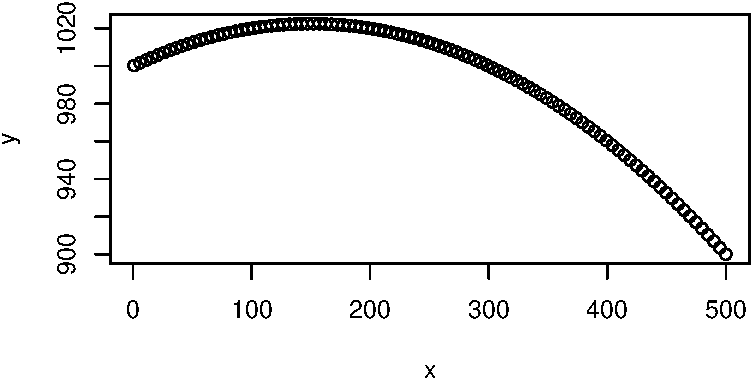
\includegraphics{022_vectors_files/figure-pdf/unnamed-chunk-48-1.pdf}

\begin{Shaded}
\begin{Highlighting}[]


\CommentTok{\#although you could use curve() here as well:}
\FunctionTok{curve}\NormalTok{(}\DecValTok{1000} \SpecialCharTok{{-}} \FloatTok{0.001}\SpecialCharTok{*}\NormalTok{x}\SpecialCharTok{\^{}}\DecValTok{2} \SpecialCharTok{+} \FloatTok{0.3}\SpecialCharTok{*}\NormalTok{x, }\AttributeTok{from=}\DecValTok{1}\NormalTok{, }\AttributeTok{to=}\DecValTok{500}\NormalTok{)}
\end{Highlighting}
\end{Shaded}

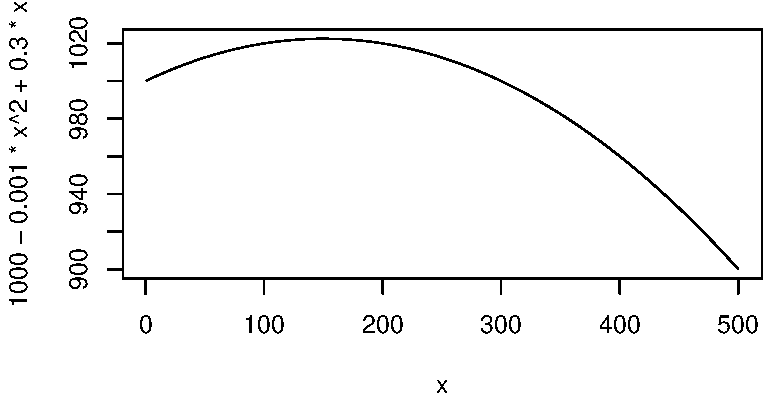
\includegraphics{022_vectors_files/figure-pdf/unnamed-chunk-48-2.pdf}

\chapter{Data frames and lists}\label{sec-data-frames-and-lists}

\section{Data frames}\label{data-frames}

\subsection{A Data frame \ldots{} your beloved
spreadsheet}\label{a-data-frame-your-beloved-spreadsheet}

\begin{Shaded}
\begin{Highlighting}[]
\NormalTok{df}\OtherTok{\textless{}{-}}\FunctionTok{data.frame}\NormalTok{() }\CommentTok{\#an empty one}

\NormalTok{df}\OtherTok{\textless{}{-}}\FunctionTok{data.frame}\NormalTok{(}\AttributeTok{a =} \DecValTok{1}\SpecialCharTok{:}\DecValTok{5}\NormalTok{,}
           \AttributeTok{b =}\NormalTok{ letters[}\DecValTok{1}\SpecialCharTok{:}\DecValTok{5}\NormalTok{],}
           \AttributeTok{c =} \FunctionTok{rnorm}\NormalTok{(}\AttributeTok{n =} \DecValTok{5}\NormalTok{))}
\NormalTok{df}
\CommentTok{\#\textgreater{}   a b           c}
\CommentTok{\#\textgreater{} 1 1 a  0.80176019}
\CommentTok{\#\textgreater{} 2 2 b  0.01083657}
\CommentTok{\#\textgreater{} 3 3 c {-}1.58018304}
\CommentTok{\#\textgreater{} 4 4 d  0.49265849}
\CommentTok{\#\textgreater{} 5 5 e  0.72350814}
\end{Highlighting}
\end{Shaded}

See how it is summarized. Basically summarizing each vector in columns.

\begin{Shaded}
\begin{Highlighting}[]
\FunctionTok{summary}\NormalTok{(df)}
\CommentTok{\#\textgreater{}        a          b                   c           }
\CommentTok{\#\textgreater{}  Min.   :1   Length:5           Min.   :{-}1.58018  }
\CommentTok{\#\textgreater{}  1st Qu.:2   Class :character   1st Qu.: 0.01084  }
\CommentTok{\#\textgreater{}  Median :3   Mode  :character   Median : 0.49266  }
\CommentTok{\#\textgreater{}  Mean   :3                      Mean   : 0.08972  }
\CommentTok{\#\textgreater{}  3rd Qu.:4                      3rd Qu.: 0.72351  }
\CommentTok{\#\textgreater{}  Max.   :5                      Max.   : 0.80176}
\end{Highlighting}
\end{Shaded}

\subsection{Accessing and subsetting}\label{accessing-and-subsetting}

\textbf{!!! THIS IS EXTREMELY IMPORTANT !!!} \textbf{!!! Don't forget
the comma}

Identifying

\begin{Shaded}
\begin{Highlighting}[]
\NormalTok{df[,}\StringTok{"b"}\NormalTok{] }\CommentTok{\#all rows but only the column named "b"}
\CommentTok{\#\textgreater{} [1] "a" "b" "c" "d" "e"}
\NormalTok{df}\SpecialCharTok{$}\NormalTok{b }\CommentTok{\#same !}
\CommentTok{\#\textgreater{} [1] "a" "b" "c" "d" "e"}
\end{Highlighting}
\end{Shaded}

Subsetting based on position

\begin{Shaded}
\begin{Highlighting}[]
\NormalTok{df}\SpecialCharTok{$}\NormalTok{c[}\DecValTok{1}\SpecialCharTok{:}\DecValTok{2}\NormalTok{] }\CommentTok{\#subsetting a vector: only first 2 values}
\CommentTok{\#\textgreater{} [1] 0.80176019 0.01083657}
\NormalTok{df[}\DecValTok{1}\SpecialCharTok{:}\DecValTok{2}\NormalTok{,}\StringTok{"b"}\NormalTok{]}
\CommentTok{\#\textgreater{} [1] "a" "b"}
\NormalTok{df[}\DecValTok{1}\SpecialCharTok{:}\DecValTok{2}\NormalTok{,] }\CommentTok{\#first 2 records, all variables. Don\textquotesingle{}t forget the comma !}
\CommentTok{\#\textgreater{}   a b          c}
\CommentTok{\#\textgreater{} 1 1 a 0.80176019}
\CommentTok{\#\textgreater{} 2 2 b 0.01083657}
\end{Highlighting}
\end{Shaded}

Subsetting specific rows (not range as above):

\begin{Shaded}
\begin{Highlighting}[]
\NormalTok{df[}\DecValTok{1}\SpecialCharTok{:}\DecValTok{3}\NormalTok{,}\StringTok{"b"}\NormalTok{]}
\CommentTok{\#\textgreater{} [1] "a" "b" "c"}
\NormalTok{df[}\FunctionTok{c}\NormalTok{(}\DecValTok{1}\NormalTok{,}\DecValTok{3}\NormalTok{),}\StringTok{"b"}\NormalTok{]}
\CommentTok{\#\textgreater{} [1] "a" "c"}
\end{Highlighting}
\end{Shaded}

Each dataframe column must have the same number of elements.

(Enjoy this condition after thinking of how many times you had
misaligned and columns of different lengths in Ms Exc..)

\begin{Shaded}
\begin{Highlighting}[]
\NormalTok{z}\OtherTok{\textless{}{-}}\FunctionTok{c}\NormalTok{(}\StringTok{"Mom"}\NormalTok{,}\StringTok{"Dad"}\NormalTok{,}\DecValTok{3}\NormalTok{) }\CommentTok{\#remember each vector as only one type of data, so this is coerced to character}

\NormalTok{df}\SpecialCharTok{$}\NormalTok{z}\OtherTok{\textless{}{-}}\NormalTok{z }\CommentTok{\#Should not work becouse of different length}
\CommentTok{\#\textgreater{} Error in \textasciigrave{}$\textless{}{-}.data.frame\textasciigrave{}(\textasciigrave{}*tmp*\textasciigrave{}, z, value = c("Mom", "Dad", "3")): replacement has 3 rows, data has 5}
\end{Highlighting}
\end{Shaded}

\begin{Shaded}
\begin{Highlighting}[]
\FunctionTok{length}\NormalTok{(df}\SpecialCharTok{$}\NormalTok{a)}
\CommentTok{\#\textgreater{} [1] 5}
\FunctionTok{length}\NormalTok{(z)}
\CommentTok{\#\textgreater{} [1] 3}

\CommentTok{\#Beware. Length applied to the whole df means the number of columns!}
\FunctionTok{length}\NormalTok{(df) }\CommentTok{\#i.e. a b and c}
\CommentTok{\#\textgreater{} [1] 3}
\end{Highlighting}
\end{Shaded}

While length is general, for a data frame you can rather compute number
of rows and columns this way

\begin{Shaded}
\begin{Highlighting}[]
\FunctionTok{nrow}\NormalTok{(df)}
\CommentTok{\#\textgreater{} [1] 5}
\FunctionTok{ncol}\NormalTok{(df)}
\CommentTok{\#\textgreater{} [1] 3}
\FunctionTok{dim}\NormalTok{(df)}
\CommentTok{\#\textgreater{} [1] 5 3}
\FunctionTok{nrow}\NormalTok{(df)}\SpecialCharTok{==}\FunctionTok{dim}\NormalTok{(df)[}\DecValTok{2}\NormalTok{] }\CommentTok{\#What do you think?}
\CommentTok{\#\textgreater{} [1] FALSE}

\CommentTok{\#But these won\textquotesingle{}t work for a vector:}
\FunctionTok{dim}\NormalTok{(df}\SpecialCharTok{$}\NormalTok{a)}
\CommentTok{\#\textgreater{} NULL}
\FunctionTok{nrow}\NormalTok{(df}\SpecialCharTok{$}\NormalTok{a)}
\CommentTok{\#\textgreater{} NULL}
\end{Highlighting}
\end{Shaded}

Often times data frames have more complicated column names. It is useful
to access those directly.

This is also the way you change the name of a column:

\begin{Shaded}
\begin{Highlighting}[]
\FunctionTok{names}\NormalTok{(df)[}\DecValTok{2}\NormalTok{]}\OtherTok{\textless{}{-}}\StringTok{"blabla"}
\NormalTok{df}
\CommentTok{\#\textgreater{}   a blabla           c}
\CommentTok{\#\textgreater{} 1 1      a  0.80176019}
\CommentTok{\#\textgreater{} 2 2      b  0.01083657}
\CommentTok{\#\textgreater{} 3 3      c {-}1.58018304}
\CommentTok{\#\textgreater{} 4 4      d  0.49265849}
\CommentTok{\#\textgreater{} 5 5      e  0.72350814}
\end{Highlighting}
\end{Shaded}

\section{Lists}\label{lists}

A List is a more general object than a dataframe.

All ``columns'' are not necessarily

\begin{itemize}
\tightlist
\item
  of the same length
\item
  nor of the same class
\end{itemize}

\begin{Shaded}
\begin{Highlighting}[]
\NormalTok{mylist}\OtherTok{\textless{}{-}}\FunctionTok{list}\NormalTok{(}\AttributeTok{a =} \DecValTok{1}\SpecialCharTok{:}\DecValTok{5}\NormalTok{,}
             \AttributeTok{b =}\NormalTok{ letters[}\DecValTok{1}\SpecialCharTok{:}\DecValTok{5}\NormalTok{],}
             \AttributeTok{c =} \FunctionTok{rnorm}\NormalTok{(}\AttributeTok{n =} \DecValTok{5}\NormalTok{))}
\NormalTok{mylist}
\CommentTok{\#\textgreater{} $a}
\CommentTok{\#\textgreater{} [1] 1 2 3 4 5}
\CommentTok{\#\textgreater{} }
\CommentTok{\#\textgreater{} $b}
\CommentTok{\#\textgreater{} [1] "a" "b" "c" "d" "e"}
\CommentTok{\#\textgreater{} }
\CommentTok{\#\textgreater{} $c}
\CommentTok{\#\textgreater{} [1] {-}1.0267704 {-}2.1750821 {-}1.4611886  0.3560756 {-}0.8646399}
\FunctionTok{summary}\NormalTok{(mylist)}
\CommentTok{\#\textgreater{}   Length Class  Mode     }
\CommentTok{\#\textgreater{} a 5      {-}none{-} numeric  }
\CommentTok{\#\textgreater{} b 5      {-}none{-} character}
\CommentTok{\#\textgreater{} c 5      {-}none{-} numeric}
\end{Highlighting}
\end{Shaded}

\begin{Shaded}
\begin{Highlighting}[]
\NormalTok{mylist}\OtherTok{\textless{}{-}}\FunctionTok{list}\NormalTok{(}\AttributeTok{a =} \DecValTok{1}\SpecialCharTok{:}\DecValTok{3}\NormalTok{,}\CommentTok{\#we removed 2 elements here}
             \AttributeTok{b =}\NormalTok{ letters[}\DecValTok{1}\SpecialCharTok{:}\DecValTok{5}\NormalTok{],}
             \AttributeTok{c =} \FunctionTok{rnorm}\NormalTok{(}\AttributeTok{n =} \DecValTok{5}\NormalTok{))}
\NormalTok{mylist}
\CommentTok{\#\textgreater{} $a}
\CommentTok{\#\textgreater{} [1] 1 2 3}
\CommentTok{\#\textgreater{} }
\CommentTok{\#\textgreater{} $b}
\CommentTok{\#\textgreater{} [1] "a" "b" "c" "d" "e"}
\CommentTok{\#\textgreater{} }
\CommentTok{\#\textgreater{} $c}
\CommentTok{\#\textgreater{} [1] {-}0.2078584 {-}0.0993671 {-}0.3070506  0.8399877 {-}1.4921589}
\FunctionTok{summary}\NormalTok{(mylist)}
\CommentTok{\#\textgreater{}   Length Class  Mode     }
\CommentTok{\#\textgreater{} a 3      {-}none{-} numeric  }
\CommentTok{\#\textgreater{} b 5      {-}none{-} character}
\CommentTok{\#\textgreater{} c 5      {-}none{-} numeric}
\end{Highlighting}
\end{Shaded}

\begin{Shaded}
\begin{Highlighting}[]
\FunctionTok{length}\NormalTok{(mylist) }\CommentTok{\#number of elements in list}
\CommentTok{\#\textgreater{} [1] 3}
\FunctionTok{length}\NormalTok{(mylist}\SpecialCharTok{$}\NormalTok{b) }\CommentTok{\#number of objects within that element of the list}
\CommentTok{\#\textgreater{} [1] 5}
\end{Highlighting}
\end{Shaded}

\subsection{Into the lists: {[}{[} {]}{]} vs {[}
{]}}\label{into-the-lists-vs}

\begin{Shaded}
\begin{Highlighting}[]
\NormalTok{mylist[}\DecValTok{2}\NormalTok{] }\CommentTok{\# getting the list element displayed}
\CommentTok{\#\textgreater{} $b}
\CommentTok{\#\textgreater{} [1] "a" "b" "c" "d" "e"}
\FunctionTok{class}\NormalTok{(mylist[}\DecValTok{2}\NormalTok{])  }\CommentTok{\# you see it is a list element}
\CommentTok{\#\textgreater{} [1] "list"}
\NormalTok{mylist[[}\DecValTok{2}\NormalTok{]] }\CommentTok{\# getting the corresponding vector}
\CommentTok{\#\textgreater{} [1] "a" "b" "c" "d" "e"}
\FunctionTok{class}\NormalTok{(mylist[[}\DecValTok{2}\NormalTok{]]) }\CommentTok{\# you now see it is a character vector}
\CommentTok{\#\textgreater{} [1] "character"}
\end{Highlighting}
\end{Shaded}

And now subsetting:

\begin{Shaded}
\begin{Highlighting}[]
\NormalTok{mylist}
\CommentTok{\#\textgreater{} $a}
\CommentTok{\#\textgreater{} [1] 1 2 3}
\CommentTok{\#\textgreater{} }
\CommentTok{\#\textgreater{} $b}
\CommentTok{\#\textgreater{} [1] "a" "b" "c" "d" "e"}
\CommentTok{\#\textgreater{} }
\CommentTok{\#\textgreater{} $c}
\CommentTok{\#\textgreater{} [1] {-}0.2078584 {-}0.0993671 {-}0.3070506  0.8399877 {-}1.4921589}
\NormalTok{mylist[[}\DecValTok{2}\NormalTok{]][}\DecValTok{1}\NormalTok{] }\CommentTok{\#1st element of the 2nd element of the list}
\CommentTok{\#\textgreater{} [1] "a"}
\NormalTok{mylist[[}\DecValTok{1}\NormalTok{]][}\DecValTok{2}\NormalTok{] }\CommentTok{\#2nd element of the 1st element of the list}
\CommentTok{\#\textgreater{} [1] 2}
\NormalTok{M}\OtherTok{\textless{}{-}}\NormalTok{mylist[[}\DecValTok{3}\NormalTok{]]}
\NormalTok{M[}\DecValTok{1}\NormalTok{] }\CommentTok{\#Subsetting just as any vector}
\CommentTok{\#\textgreater{} [1] {-}0.2078584}
\end{Highlighting}
\end{Shaded}

\chapter{Working with data frames and
functions}\label{sec-working-with-data-frames-and-functions}

\section{What is in a function? BMI
example}\label{what-is-in-a-function-bmi-example}

\begin{itemize}
\item
  Let's create a BMI function
\item
  First a simple function that simply prints a given height and weight
\end{itemize}

\begin{Shaded}
\begin{Highlighting}[]
\NormalTok{paste.heightweight}\OtherTok{\textless{}{-}}\ControlFlowTok{function}\NormalTok{(h,w)\{}
  \FunctionTok{print}\NormalTok{(}\FunctionTok{paste}\NormalTok{(h,w))}
\NormalTok{  \}}
\FunctionTok{paste.heightweight}\NormalTok{(}\FloatTok{1.8}\NormalTok{,}\DecValTok{80}\NormalTok{) }\CommentTok{\#you provide the 2 arguments and get the output}
\CommentTok{\#\textgreater{} [1] "1.8 80"}
\end{Highlighting}
\end{Shaded}

Now let's do the computation with the BMI calculation with a new
function

\begin{Shaded}
\begin{Highlighting}[]
\NormalTok{bmi.calc}\OtherTok{\textless{}{-}}\ControlFlowTok{function}\NormalTok{(h,w)\{w}\SpecialCharTok{/}\NormalTok{h}\SpecialCharTok{\^{}}\DecValTok{2}\NormalTok{\}}
\end{Highlighting}
\end{Shaded}

which we apply

\begin{Shaded}
\begin{Highlighting}[]
\FunctionTok{bmi.calc}\NormalTok{(}\FloatTok{1.8}\NormalTok{,}\DecValTok{80}\NormalTok{)}
\CommentTok{\#\textgreater{} [1] 24.69136}
\end{Highlighting}
\end{Shaded}

A function can take a sequence of processes (e.g compute, rounds,
concatenate a sentence,\ldots) and then returns the result of the last
process.

Example

\begin{Shaded}
\begin{Highlighting}[]
\NormalTok{bmi.calc.text}\OtherTok{\textless{}{-}}\ControlFlowTok{function}\NormalTok{(h,w)\{}
\NormalTok{  b}\OtherTok{\textless{}{-}}\NormalTok{w}\SpecialCharTok{/}\NormalTok{h}\SpecialCharTok{\^{}}\DecValTok{2}
\NormalTok{  brounded}\OtherTok{\textless{}{-}}\FunctionTok{round}\NormalTok{(b)}
  \FunctionTok{paste}\NormalTok{(}\StringTok{"My BMI is"}\NormalTok{, brounded, }\StringTok{"kg/m2"}\NormalTok{)}
\NormalTok{\}}
\FunctionTok{bmi.calc.text}\NormalTok{(}\FloatTok{1.8}\NormalTok{,}\DecValTok{80}\NormalTok{)}
\CommentTok{\#\textgreater{} [1] "My BMI is 25 kg/m2"}
\end{Highlighting}
\end{Shaded}

For clarity the outcome of the function can be put in a return()

\begin{Shaded}
\begin{Highlighting}[]
\NormalTok{bmi.calc}\OtherTok{\textless{}{-}}\ControlFlowTok{function}\NormalTok{(h,w)\{}
  \FunctionTok{return}\NormalTok{(}\FunctionTok{round}\NormalTok{(w}\SpecialCharTok{/}\NormalTok{h}\SpecialCharTok{\^{}}\DecValTok{2}\NormalTok{))}
\NormalTok{\}}
\FunctionTok{bmi.calc}\NormalTok{(}\FloatTok{1.8}\NormalTok{,}\DecValTok{80}\NormalTok{)}
\CommentTok{\#\textgreater{} [1] 25}
\end{Highlighting}
\end{Shaded}

\section{Applying a function to a data frame
column}\label{applying-a-function-to-a-data-frame-column}

Let's create a 2nd function to transfors degrees from Celsius to
Fahrenheit

Simpler with a single argument (x):

\begin{Shaded}
\begin{Highlighting}[]
\NormalTok{celsius2fahrenheit}\OtherTok{\textless{}{-}}\ControlFlowTok{function}\NormalTok{(x)\{}\FunctionTok{round}\NormalTok{(}\DecValTok{32}\SpecialCharTok{+}\NormalTok{(x}\SpecialCharTok{*}\DecValTok{9}\SpecialCharTok{/}\DecValTok{5}\NormalTok{))\}}

\FunctionTok{celsius2fahrenheit}\NormalTok{(}\DecValTok{25}\NormalTok{) }\CommentTok{\#25 celsius degree is thus }
\CommentTok{\#\textgreater{} [1] 77}
\end{Highlighting}
\end{Shaded}

Which we now apply to a series of values stored in a column within a
data frame

\begin{Shaded}
\begin{Highlighting}[]
\NormalTok{mytable}\OtherTok{\textless{}{-}}\FunctionTok{data.frame}\NormalTok{(}\AttributeTok{A=}\FunctionTok{c}\NormalTok{(}\DecValTok{21}\NormalTok{,}\DecValTok{22}\NormalTok{,}\DecValTok{23}\NormalTok{,}\DecValTok{24}\NormalTok{,}\DecValTok{25}\NormalTok{,}\DecValTok{26}\NormalTok{,}\DecValTok{27}\NormalTok{))}
\NormalTok{mytable}\SpecialCharTok{$}\NormalTok{F}\OtherTok{\textless{}{-}}\FunctionTok{celsius2fahrenheit}\NormalTok{(mytable[,}\StringTok{"A"}\NormalTok{])}
\NormalTok{mytable}
\CommentTok{\#\textgreater{}    A  F}
\CommentTok{\#\textgreater{} 1 21 70}
\CommentTok{\#\textgreater{} 2 22 72}
\CommentTok{\#\textgreater{} 3 23 73}
\CommentTok{\#\textgreater{} 4 24 75}
\CommentTok{\#\textgreater{} 5 25 77}
\CommentTok{\#\textgreater{} 6 26 79}
\CommentTok{\#\textgreater{} 7 27 81}
\end{Highlighting}
\end{Shaded}

\section{Data frames and NA's}\label{data-frames-and-nas}

Computation of a new column from columns of a dataframe

\begin{Shaded}
\begin{Highlighting}[]
\NormalTok{mytable}\SpecialCharTok{$}\NormalTok{G}\OtherTok{\textless{}{-}}\NormalTok{mytable}\SpecialCharTok{$}\NormalTok{A}\SpecialCharTok{+}\NormalTok{mytable}\SpecialCharTok{$}\NormalTok{F }\CommentTok{\#note: adding C and F temperature is nonsensical though}
\NormalTok{mytable}\SpecialCharTok{$}\NormalTok{Gsquare}\OtherTok{\textless{}{-}}\NormalTok{mytable}\SpecialCharTok{$}\NormalTok{G}\SpecialCharTok{\^{}}\DecValTok{2} \CommentTok{\#note how you write an exponent "\^{}" in R}
\NormalTok{mytable}\SpecialCharTok{$}\NormalTok{A}\SpecialCharTok{*}\NormalTok{mytable}\SpecialCharTok{$}\NormalTok{F }\CommentTok{\# or a multiplication "*"}
\CommentTok{\#\textgreater{} [1] 1470 1584 1679 1800 1925 2054 2187}
\end{Highlighting}
\end{Shaded}

Similarly we can apply our BMI computation to a data frame with heights
and weights

\begin{Shaded}
\begin{Highlighting}[]
\NormalTok{bmidf}\OtherTok{\textless{}{-}}\FunctionTok{data.frame}\NormalTok{(}
  \AttributeTok{h=}\FunctionTok{c}\NormalTok{(}\FloatTok{1.8}\NormalTok{,}\FloatTok{1.7}\NormalTok{,}\DecValTok{2}\NormalTok{,}\FloatTok{1.9}\NormalTok{),}
  \AttributeTok{w=}\FunctionTok{c}\NormalTok{(}\DecValTok{70}\NormalTok{,}\DecValTok{70}\NormalTok{,}\DecValTok{95}\NormalTok{,}\DecValTok{100}\NormalTok{))}
\end{Highlighting}
\end{Shaded}

We add the result of computing BMI directly as a new column ``BMI'' in
our data.frame

\begin{Shaded}
\begin{Highlighting}[]
\NormalTok{bmidf}\SpecialCharTok{$}\NormalTok{BMI}\OtherTok{\textless{}{-}}\FunctionTok{bmi.calc}\NormalTok{(}\AttributeTok{h=}\NormalTok{bmidf}\SpecialCharTok{$}\NormalTok{h,}
                    \AttributeTok{w=}\NormalTok{bmidf}\SpecialCharTok{$}\NormalTok{w)}
\end{Highlighting}
\end{Shaded}

NA is for unknowns !

Suppose the 2nd person of our sample didn't share his/her weight with us

\begin{Shaded}
\begin{Highlighting}[]
\NormalTok{bmidf}\SpecialCharTok{$}\NormalTok{w[}\DecValTok{2}\NormalTok{]}\OtherTok{\textless{}{-}}\ConstantTok{NA} \CommentTok{\#NA is for unknowns}
\NormalTok{bmidf}\SpecialCharTok{$}\NormalTok{BMI}\OtherTok{\textless{}{-}}\FunctionTok{bmi.calc}\NormalTok{(}\AttributeTok{h=}\NormalTok{bmidf}\SpecialCharTok{$}\NormalTok{h,}
                    \AttributeTok{w=}\NormalTok{bmidf}\SpecialCharTok{$}\NormalTok{w)}
\CommentTok{\#You see the BMI could therefore not be computed}
\NormalTok{bmidf}
\CommentTok{\#\textgreater{}     h   w BMI}
\CommentTok{\#\textgreater{} 1 1.8  70  22}
\CommentTok{\#\textgreater{} 2 1.7  NA  NA}
\CommentTok{\#\textgreater{} 3 2.0  95  24}
\CommentTok{\#\textgreater{} 4 1.9 100  28}
\end{Highlighting}
\end{Shaded}

For some functions you would still want to compute a value while
ignoring the NA's

The mean is a classical example

\begin{Shaded}
\begin{Highlighting}[]
\FunctionTok{mean}\NormalTok{(bmidf}\SpecialCharTok{$}\NormalTok{h) }\CommentTok{\#works}
\CommentTok{\#\textgreater{} [1] 1.85}
\FunctionTok{mean}\NormalTok{(bmidf}\SpecialCharTok{$}\NormalTok{w) }\CommentTok{\#but returns NA because of one value not reported}
\CommentTok{\#\textgreater{} [1] NA}
\end{Highlighting}
\end{Shaded}

You can explicitly ask to compute without the NA's:

\begin{Shaded}
\begin{Highlighting}[]
\FunctionTok{mean}\NormalTok{(bmidf}\SpecialCharTok{$}\NormalTok{w, }\AttributeTok{na.rm=}\ConstantTok{TRUE}\NormalTok{) }\CommentTok{\#now works!}
\CommentTok{\#\textgreater{} [1] 88.33333}
\end{Highlighting}
\end{Shaded}

Using complete cases

For some data frame made of surveyed values where different variables
are filled in sparsely, it is important you get access only to entirely
completed individuals

\begin{Shaded}
\begin{Highlighting}[]
\FunctionTok{complete.cases}\NormalTok{(bmidf) }\CommentTok{\#returns a logical indicating whether the row }
\CommentTok{\#\textgreater{} [1]  TRUE FALSE  TRUE  TRUE}
\CommentTok{\# has not a singleNA}
\FunctionTok{class}\NormalTok{(}\FunctionTok{complete.cases}\NormalTok{(bmidf))}
\CommentTok{\#\textgreater{} [1] "logical"}
\CommentTok{\#Note that with logicals, TRUE is 1 and FALSE is zero. Thus}

\FunctionTok{sum}\NormalTok{(}\FunctionTok{complete.cases}\NormalTok{(bmidf))}
\CommentTok{\#\textgreater{} [1] 3}

\CommentTok{\#You can use this logical to subset the rows}
\CommentTok{\# and have a "clean" df}
\NormalTok{bmidf2}\OtherTok{\textless{}{-}}\NormalTok{bmidf[}\FunctionTok{complete.cases}\NormalTok{(bmidf),] }\CommentTok{\#read this as "select complete cases rows with all columns}
\NormalTok{bmidf2}
\CommentTok{\#\textgreater{}     h   w BMI}
\CommentTok{\#\textgreater{} 1 1.8  70  22}
\CommentTok{\#\textgreater{} 3 2.0  95  24}
\CommentTok{\#\textgreater{} 4 1.9 100  28}
\end{Highlighting}
\end{Shaded}

\section{Environment listing and
management}\label{environment-listing-and-management}

We have now created a bunch of objects which we can see in the
Environment window of RStudio.

In the console we can also see them with

\begin{Shaded}
\begin{Highlighting}[]
\FunctionTok{ls}\NormalTok{()}
\CommentTok{\#\textgreater{} [1] "bmi.calc"           "bmi.calc.text"      "bmidf"             }
\CommentTok{\#\textgreater{} [4] "bmidf2"             "celsius2fahrenheit" "mytable"           }
\CommentTok{\#\textgreater{} [7] "paste.heightweight"}
\end{Highlighting}
\end{Shaded}

And any of these objects can be removed with

\begin{Shaded}
\begin{Highlighting}[]
\FunctionTok{rm}\NormalTok{()}
\CommentTok{\#for example}
\FunctionTok{rm}\NormalTok{(mytable)}
\end{Highlighting}
\end{Shaded}

In the environment window of RStudio you also see the structure of
objects (when displayed as a list not a grid)

From the console you use the structure function str() to get the same
info

\begin{Shaded}
\begin{Highlighting}[]
\FunctionTok{str}\NormalTok{(bmidf)}
\CommentTok{\#\textgreater{} \textquotesingle{}data.frame\textquotesingle{}:    4 obs. of  3 variables:}
\CommentTok{\#\textgreater{}  $ h  : num  1.8 1.7 2 1.9}
\CommentTok{\#\textgreater{}  $ w  : num  70 NA 95 100}
\CommentTok{\#\textgreater{}  $ BMI: num  22 NA 24 28}
\end{Highlighting}
\end{Shaded}

\section{Viewing data frame}\label{viewing-data-frame}

\begin{Shaded}
\begin{Highlighting}[]
\FunctionTok{View}\NormalTok{(bmidf)}
\end{Highlighting}
\end{Shaded}

is the most pleasant interactive way to view a data frame

But be careful if many rows or columns !

The classical console way is simply

\begin{Shaded}
\begin{Highlighting}[]
\NormalTok{bmidf}
\CommentTok{\#\textgreater{}     h   w BMI}
\CommentTok{\#\textgreater{} 1 1.8  70  22}
\CommentTok{\#\textgreater{} 2 1.7  NA  NA}
\CommentTok{\#\textgreater{} 3 2.0  95  24}
\CommentTok{\#\textgreater{} 4 1.9 100  28}
\end{Highlighting}
\end{Shaded}

In case of a large vector or df there will be a limited display of 1000
values (default) in console

Suppose you have a vector of 1002 values

\begin{Shaded}
\begin{Highlighting}[]
\NormalTok{mydf}\OtherTok{\textless{}{-}}\FunctionTok{data.frame}\NormalTok{(}\AttributeTok{z=}\DecValTok{1}\SpecialCharTok{:}\DecValTok{502}\NormalTok{, }\AttributeTok{zrev=}\DecValTok{502}\SpecialCharTok{:}\DecValTok{1}\NormalTok{)}
\NormalTok{mydf}
\CommentTok{\#\textgreater{}       z zrev}
\CommentTok{\#\textgreater{} 1     1  502}
\CommentTok{\#\textgreater{} 2     2  501}
\CommentTok{\#\textgreater{} 3     3  500}
\CommentTok{\#\textgreater{} 4     4  499}
\CommentTok{\#\textgreater{} 5     5  498}
\CommentTok{\#\textgreater{} 6     6  497}
\CommentTok{\#\textgreater{} 7     7  496}
\CommentTok{\#\textgreater{} 8     8  495}
\CommentTok{\#\textgreater{} 9     9  494}
\CommentTok{\#\textgreater{} 10   10  493}
\CommentTok{\#\textgreater{} 11   11  492}
\CommentTok{\#\textgreater{} 12   12  491}
\CommentTok{\#\textgreater{} 13   13  490}
\CommentTok{\#\textgreater{} 14   14  489}
\CommentTok{\#\textgreater{} 15   15  488}
\CommentTok{\#\textgreater{} 16   16  487}
\CommentTok{\#\textgreater{} 17   17  486}
\CommentTok{\#\textgreater{} 18   18  485}
\CommentTok{\#\textgreater{} 19   19  484}
\CommentTok{\#\textgreater{} 20   20  483}
\CommentTok{\#\textgreater{} 21   21  482}
\CommentTok{\#\textgreater{} 22   22  481}
\CommentTok{\#\textgreater{} 23   23  480}
\CommentTok{\#\textgreater{} 24   24  479}
\CommentTok{\#\textgreater{} 25   25  478}
\CommentTok{\#\textgreater{} 26   26  477}
\CommentTok{\#\textgreater{} 27   27  476}
\CommentTok{\#\textgreater{} 28   28  475}
\CommentTok{\#\textgreater{} 29   29  474}
\CommentTok{\#\textgreater{} 30   30  473}
\CommentTok{\#\textgreater{} 31   31  472}
\CommentTok{\#\textgreater{} 32   32  471}
\CommentTok{\#\textgreater{} 33   33  470}
\CommentTok{\#\textgreater{} 34   34  469}
\CommentTok{\#\textgreater{} 35   35  468}
\CommentTok{\#\textgreater{} 36   36  467}
\CommentTok{\#\textgreater{} 37   37  466}
\CommentTok{\#\textgreater{} 38   38  465}
\CommentTok{\#\textgreater{} 39   39  464}
\CommentTok{\#\textgreater{} 40   40  463}
\CommentTok{\#\textgreater{} 41   41  462}
\CommentTok{\#\textgreater{} 42   42  461}
\CommentTok{\#\textgreater{} 43   43  460}
\CommentTok{\#\textgreater{} 44   44  459}
\CommentTok{\#\textgreater{} 45   45  458}
\CommentTok{\#\textgreater{} 46   46  457}
\CommentTok{\#\textgreater{} 47   47  456}
\CommentTok{\#\textgreater{} 48   48  455}
\CommentTok{\#\textgreater{} 49   49  454}
\CommentTok{\#\textgreater{} 50   50  453}
\CommentTok{\#\textgreater{} 51   51  452}
\CommentTok{\#\textgreater{} 52   52  451}
\CommentTok{\#\textgreater{} 53   53  450}
\CommentTok{\#\textgreater{} 54   54  449}
\CommentTok{\#\textgreater{} 55   55  448}
\CommentTok{\#\textgreater{} 56   56  447}
\CommentTok{\#\textgreater{} 57   57  446}
\CommentTok{\#\textgreater{} 58   58  445}
\CommentTok{\#\textgreater{} 59   59  444}
\CommentTok{\#\textgreater{} 60   60  443}
\CommentTok{\#\textgreater{} 61   61  442}
\CommentTok{\#\textgreater{} 62   62  441}
\CommentTok{\#\textgreater{} 63   63  440}
\CommentTok{\#\textgreater{} 64   64  439}
\CommentTok{\#\textgreater{} 65   65  438}
\CommentTok{\#\textgreater{} 66   66  437}
\CommentTok{\#\textgreater{} 67   67  436}
\CommentTok{\#\textgreater{} 68   68  435}
\CommentTok{\#\textgreater{} 69   69  434}
\CommentTok{\#\textgreater{} 70   70  433}
\CommentTok{\#\textgreater{} 71   71  432}
\CommentTok{\#\textgreater{} 72   72  431}
\CommentTok{\#\textgreater{} 73   73  430}
\CommentTok{\#\textgreater{} 74   74  429}
\CommentTok{\#\textgreater{} 75   75  428}
\CommentTok{\#\textgreater{} 76   76  427}
\CommentTok{\#\textgreater{} 77   77  426}
\CommentTok{\#\textgreater{} 78   78  425}
\CommentTok{\#\textgreater{} 79   79  424}
\CommentTok{\#\textgreater{} 80   80  423}
\CommentTok{\#\textgreater{} 81   81  422}
\CommentTok{\#\textgreater{} 82   82  421}
\CommentTok{\#\textgreater{} 83   83  420}
\CommentTok{\#\textgreater{} 84   84  419}
\CommentTok{\#\textgreater{} 85   85  418}
\CommentTok{\#\textgreater{} 86   86  417}
\CommentTok{\#\textgreater{} 87   87  416}
\CommentTok{\#\textgreater{} 88   88  415}
\CommentTok{\#\textgreater{} 89   89  414}
\CommentTok{\#\textgreater{} 90   90  413}
\CommentTok{\#\textgreater{} 91   91  412}
\CommentTok{\#\textgreater{} 92   92  411}
\CommentTok{\#\textgreater{} 93   93  410}
\CommentTok{\#\textgreater{} 94   94  409}
\CommentTok{\#\textgreater{} 95   95  408}
\CommentTok{\#\textgreater{} 96   96  407}
\CommentTok{\#\textgreater{} 97   97  406}
\CommentTok{\#\textgreater{} 98   98  405}
\CommentTok{\#\textgreater{} 99   99  404}
\CommentTok{\#\textgreater{} 100 100  403}
\CommentTok{\#\textgreater{} 101 101  402}
\CommentTok{\#\textgreater{} 102 102  401}
\CommentTok{\#\textgreater{} 103 103  400}
\CommentTok{\#\textgreater{} 104 104  399}
\CommentTok{\#\textgreater{} 105 105  398}
\CommentTok{\#\textgreater{} 106 106  397}
\CommentTok{\#\textgreater{} 107 107  396}
\CommentTok{\#\textgreater{} 108 108  395}
\CommentTok{\#\textgreater{} 109 109  394}
\CommentTok{\#\textgreater{} 110 110  393}
\CommentTok{\#\textgreater{} 111 111  392}
\CommentTok{\#\textgreater{} 112 112  391}
\CommentTok{\#\textgreater{} 113 113  390}
\CommentTok{\#\textgreater{} 114 114  389}
\CommentTok{\#\textgreater{} 115 115  388}
\CommentTok{\#\textgreater{} 116 116  387}
\CommentTok{\#\textgreater{} 117 117  386}
\CommentTok{\#\textgreater{} 118 118  385}
\CommentTok{\#\textgreater{} 119 119  384}
\CommentTok{\#\textgreater{} 120 120  383}
\CommentTok{\#\textgreater{} 121 121  382}
\CommentTok{\#\textgreater{} 122 122  381}
\CommentTok{\#\textgreater{} 123 123  380}
\CommentTok{\#\textgreater{} 124 124  379}
\CommentTok{\#\textgreater{} 125 125  378}
\CommentTok{\#\textgreater{} 126 126  377}
\CommentTok{\#\textgreater{} 127 127  376}
\CommentTok{\#\textgreater{} 128 128  375}
\CommentTok{\#\textgreater{} 129 129  374}
\CommentTok{\#\textgreater{} 130 130  373}
\CommentTok{\#\textgreater{} 131 131  372}
\CommentTok{\#\textgreater{} 132 132  371}
\CommentTok{\#\textgreater{} 133 133  370}
\CommentTok{\#\textgreater{} 134 134  369}
\CommentTok{\#\textgreater{} 135 135  368}
\CommentTok{\#\textgreater{} 136 136  367}
\CommentTok{\#\textgreater{} 137 137  366}
\CommentTok{\#\textgreater{} 138 138  365}
\CommentTok{\#\textgreater{} 139 139  364}
\CommentTok{\#\textgreater{} 140 140  363}
\CommentTok{\#\textgreater{} 141 141  362}
\CommentTok{\#\textgreater{} 142 142  361}
\CommentTok{\#\textgreater{} 143 143  360}
\CommentTok{\#\textgreater{} 144 144  359}
\CommentTok{\#\textgreater{} 145 145  358}
\CommentTok{\#\textgreater{} 146 146  357}
\CommentTok{\#\textgreater{} 147 147  356}
\CommentTok{\#\textgreater{} 148 148  355}
\CommentTok{\#\textgreater{} 149 149  354}
\CommentTok{\#\textgreater{} 150 150  353}
\CommentTok{\#\textgreater{} 151 151  352}
\CommentTok{\#\textgreater{} 152 152  351}
\CommentTok{\#\textgreater{} 153 153  350}
\CommentTok{\#\textgreater{} 154 154  349}
\CommentTok{\#\textgreater{} 155 155  348}
\CommentTok{\#\textgreater{} 156 156  347}
\CommentTok{\#\textgreater{} 157 157  346}
\CommentTok{\#\textgreater{} 158 158  345}
\CommentTok{\#\textgreater{} 159 159  344}
\CommentTok{\#\textgreater{} 160 160  343}
\CommentTok{\#\textgreater{} 161 161  342}
\CommentTok{\#\textgreater{} 162 162  341}
\CommentTok{\#\textgreater{} 163 163  340}
\CommentTok{\#\textgreater{} 164 164  339}
\CommentTok{\#\textgreater{} 165 165  338}
\CommentTok{\#\textgreater{} 166 166  337}
\CommentTok{\#\textgreater{} 167 167  336}
\CommentTok{\#\textgreater{} 168 168  335}
\CommentTok{\#\textgreater{} 169 169  334}
\CommentTok{\#\textgreater{} 170 170  333}
\CommentTok{\#\textgreater{} 171 171  332}
\CommentTok{\#\textgreater{} 172 172  331}
\CommentTok{\#\textgreater{} 173 173  330}
\CommentTok{\#\textgreater{} 174 174  329}
\CommentTok{\#\textgreater{} 175 175  328}
\CommentTok{\#\textgreater{} 176 176  327}
\CommentTok{\#\textgreater{} 177 177  326}
\CommentTok{\#\textgreater{} 178 178  325}
\CommentTok{\#\textgreater{} 179 179  324}
\CommentTok{\#\textgreater{} 180 180  323}
\CommentTok{\#\textgreater{} 181 181  322}
\CommentTok{\#\textgreater{} 182 182  321}
\CommentTok{\#\textgreater{} 183 183  320}
\CommentTok{\#\textgreater{} 184 184  319}
\CommentTok{\#\textgreater{} 185 185  318}
\CommentTok{\#\textgreater{} 186 186  317}
\CommentTok{\#\textgreater{} 187 187  316}
\CommentTok{\#\textgreater{} 188 188  315}
\CommentTok{\#\textgreater{} 189 189  314}
\CommentTok{\#\textgreater{} 190 190  313}
\CommentTok{\#\textgreater{} 191 191  312}
\CommentTok{\#\textgreater{} 192 192  311}
\CommentTok{\#\textgreater{} 193 193  310}
\CommentTok{\#\textgreater{} 194 194  309}
\CommentTok{\#\textgreater{} 195 195  308}
\CommentTok{\#\textgreater{} 196 196  307}
\CommentTok{\#\textgreater{} 197 197  306}
\CommentTok{\#\textgreater{} 198 198  305}
\CommentTok{\#\textgreater{} 199 199  304}
\CommentTok{\#\textgreater{} 200 200  303}
\CommentTok{\#\textgreater{} 201 201  302}
\CommentTok{\#\textgreater{} 202 202  301}
\CommentTok{\#\textgreater{} 203 203  300}
\CommentTok{\#\textgreater{} 204 204  299}
\CommentTok{\#\textgreater{} 205 205  298}
\CommentTok{\#\textgreater{} 206 206  297}
\CommentTok{\#\textgreater{} 207 207  296}
\CommentTok{\#\textgreater{} 208 208  295}
\CommentTok{\#\textgreater{} 209 209  294}
\CommentTok{\#\textgreater{} 210 210  293}
\CommentTok{\#\textgreater{} 211 211  292}
\CommentTok{\#\textgreater{} 212 212  291}
\CommentTok{\#\textgreater{} 213 213  290}
\CommentTok{\#\textgreater{} 214 214  289}
\CommentTok{\#\textgreater{} 215 215  288}
\CommentTok{\#\textgreater{} 216 216  287}
\CommentTok{\#\textgreater{} 217 217  286}
\CommentTok{\#\textgreater{} 218 218  285}
\CommentTok{\#\textgreater{} 219 219  284}
\CommentTok{\#\textgreater{} 220 220  283}
\CommentTok{\#\textgreater{} 221 221  282}
\CommentTok{\#\textgreater{} 222 222  281}
\CommentTok{\#\textgreater{} 223 223  280}
\CommentTok{\#\textgreater{} 224 224  279}
\CommentTok{\#\textgreater{} 225 225  278}
\CommentTok{\#\textgreater{} 226 226  277}
\CommentTok{\#\textgreater{} 227 227  276}
\CommentTok{\#\textgreater{} 228 228  275}
\CommentTok{\#\textgreater{} 229 229  274}
\CommentTok{\#\textgreater{} 230 230  273}
\CommentTok{\#\textgreater{} 231 231  272}
\CommentTok{\#\textgreater{} 232 232  271}
\CommentTok{\#\textgreater{} 233 233  270}
\CommentTok{\#\textgreater{} 234 234  269}
\CommentTok{\#\textgreater{} 235 235  268}
\CommentTok{\#\textgreater{} 236 236  267}
\CommentTok{\#\textgreater{} 237 237  266}
\CommentTok{\#\textgreater{} 238 238  265}
\CommentTok{\#\textgreater{} 239 239  264}
\CommentTok{\#\textgreater{} 240 240  263}
\CommentTok{\#\textgreater{} 241 241  262}
\CommentTok{\#\textgreater{} 242 242  261}
\CommentTok{\#\textgreater{} 243 243  260}
\CommentTok{\#\textgreater{} 244 244  259}
\CommentTok{\#\textgreater{} 245 245  258}
\CommentTok{\#\textgreater{} 246 246  257}
\CommentTok{\#\textgreater{} 247 247  256}
\CommentTok{\#\textgreater{} 248 248  255}
\CommentTok{\#\textgreater{} 249 249  254}
\CommentTok{\#\textgreater{} 250 250  253}
\CommentTok{\#\textgreater{} 251 251  252}
\CommentTok{\#\textgreater{} 252 252  251}
\CommentTok{\#\textgreater{} 253 253  250}
\CommentTok{\#\textgreater{} 254 254  249}
\CommentTok{\#\textgreater{} 255 255  248}
\CommentTok{\#\textgreater{} 256 256  247}
\CommentTok{\#\textgreater{} 257 257  246}
\CommentTok{\#\textgreater{} 258 258  245}
\CommentTok{\#\textgreater{} 259 259  244}
\CommentTok{\#\textgreater{} 260 260  243}
\CommentTok{\#\textgreater{} 261 261  242}
\CommentTok{\#\textgreater{} 262 262  241}
\CommentTok{\#\textgreater{} 263 263  240}
\CommentTok{\#\textgreater{} 264 264  239}
\CommentTok{\#\textgreater{} 265 265  238}
\CommentTok{\#\textgreater{} 266 266  237}
\CommentTok{\#\textgreater{} 267 267  236}
\CommentTok{\#\textgreater{} 268 268  235}
\CommentTok{\#\textgreater{} 269 269  234}
\CommentTok{\#\textgreater{} 270 270  233}
\CommentTok{\#\textgreater{} 271 271  232}
\CommentTok{\#\textgreater{} 272 272  231}
\CommentTok{\#\textgreater{} 273 273  230}
\CommentTok{\#\textgreater{} 274 274  229}
\CommentTok{\#\textgreater{} 275 275  228}
\CommentTok{\#\textgreater{} 276 276  227}
\CommentTok{\#\textgreater{} 277 277  226}
\CommentTok{\#\textgreater{} 278 278  225}
\CommentTok{\#\textgreater{} 279 279  224}
\CommentTok{\#\textgreater{} 280 280  223}
\CommentTok{\#\textgreater{} 281 281  222}
\CommentTok{\#\textgreater{} 282 282  221}
\CommentTok{\#\textgreater{} 283 283  220}
\CommentTok{\#\textgreater{} 284 284  219}
\CommentTok{\#\textgreater{} 285 285  218}
\CommentTok{\#\textgreater{} 286 286  217}
\CommentTok{\#\textgreater{} 287 287  216}
\CommentTok{\#\textgreater{} 288 288  215}
\CommentTok{\#\textgreater{} 289 289  214}
\CommentTok{\#\textgreater{} 290 290  213}
\CommentTok{\#\textgreater{} 291 291  212}
\CommentTok{\#\textgreater{} 292 292  211}
\CommentTok{\#\textgreater{} 293 293  210}
\CommentTok{\#\textgreater{} 294 294  209}
\CommentTok{\#\textgreater{} 295 295  208}
\CommentTok{\#\textgreater{} 296 296  207}
\CommentTok{\#\textgreater{} 297 297  206}
\CommentTok{\#\textgreater{} 298 298  205}
\CommentTok{\#\textgreater{} 299 299  204}
\CommentTok{\#\textgreater{} 300 300  203}
\CommentTok{\#\textgreater{} 301 301  202}
\CommentTok{\#\textgreater{} 302 302  201}
\CommentTok{\#\textgreater{} 303 303  200}
\CommentTok{\#\textgreater{} 304 304  199}
\CommentTok{\#\textgreater{} 305 305  198}
\CommentTok{\#\textgreater{} 306 306  197}
\CommentTok{\#\textgreater{} 307 307  196}
\CommentTok{\#\textgreater{} 308 308  195}
\CommentTok{\#\textgreater{} 309 309  194}
\CommentTok{\#\textgreater{} 310 310  193}
\CommentTok{\#\textgreater{} 311 311  192}
\CommentTok{\#\textgreater{} 312 312  191}
\CommentTok{\#\textgreater{} 313 313  190}
\CommentTok{\#\textgreater{} 314 314  189}
\CommentTok{\#\textgreater{} 315 315  188}
\CommentTok{\#\textgreater{} 316 316  187}
\CommentTok{\#\textgreater{} 317 317  186}
\CommentTok{\#\textgreater{} 318 318  185}
\CommentTok{\#\textgreater{} 319 319  184}
\CommentTok{\#\textgreater{} 320 320  183}
\CommentTok{\#\textgreater{} 321 321  182}
\CommentTok{\#\textgreater{} 322 322  181}
\CommentTok{\#\textgreater{} 323 323  180}
\CommentTok{\#\textgreater{} 324 324  179}
\CommentTok{\#\textgreater{} 325 325  178}
\CommentTok{\#\textgreater{} 326 326  177}
\CommentTok{\#\textgreater{} 327 327  176}
\CommentTok{\#\textgreater{} 328 328  175}
\CommentTok{\#\textgreater{} 329 329  174}
\CommentTok{\#\textgreater{} 330 330  173}
\CommentTok{\#\textgreater{} 331 331  172}
\CommentTok{\#\textgreater{} 332 332  171}
\CommentTok{\#\textgreater{} 333 333  170}
\CommentTok{\#\textgreater{} 334 334  169}
\CommentTok{\#\textgreater{} 335 335  168}
\CommentTok{\#\textgreater{} 336 336  167}
\CommentTok{\#\textgreater{} 337 337  166}
\CommentTok{\#\textgreater{} 338 338  165}
\CommentTok{\#\textgreater{} 339 339  164}
\CommentTok{\#\textgreater{} 340 340  163}
\CommentTok{\#\textgreater{} 341 341  162}
\CommentTok{\#\textgreater{} 342 342  161}
\CommentTok{\#\textgreater{} 343 343  160}
\CommentTok{\#\textgreater{} 344 344  159}
\CommentTok{\#\textgreater{} 345 345  158}
\CommentTok{\#\textgreater{} 346 346  157}
\CommentTok{\#\textgreater{} 347 347  156}
\CommentTok{\#\textgreater{} 348 348  155}
\CommentTok{\#\textgreater{} 349 349  154}
\CommentTok{\#\textgreater{} 350 350  153}
\CommentTok{\#\textgreater{} 351 351  152}
\CommentTok{\#\textgreater{} 352 352  151}
\CommentTok{\#\textgreater{} 353 353  150}
\CommentTok{\#\textgreater{} 354 354  149}
\CommentTok{\#\textgreater{} 355 355  148}
\CommentTok{\#\textgreater{} 356 356  147}
\CommentTok{\#\textgreater{} 357 357  146}
\CommentTok{\#\textgreater{} 358 358  145}
\CommentTok{\#\textgreater{} 359 359  144}
\CommentTok{\#\textgreater{} 360 360  143}
\CommentTok{\#\textgreater{} 361 361  142}
\CommentTok{\#\textgreater{} 362 362  141}
\CommentTok{\#\textgreater{} 363 363  140}
\CommentTok{\#\textgreater{} 364 364  139}
\CommentTok{\#\textgreater{} 365 365  138}
\CommentTok{\#\textgreater{} 366 366  137}
\CommentTok{\#\textgreater{} 367 367  136}
\CommentTok{\#\textgreater{} 368 368  135}
\CommentTok{\#\textgreater{} 369 369  134}
\CommentTok{\#\textgreater{} 370 370  133}
\CommentTok{\#\textgreater{} 371 371  132}
\CommentTok{\#\textgreater{} 372 372  131}
\CommentTok{\#\textgreater{} 373 373  130}
\CommentTok{\#\textgreater{} 374 374  129}
\CommentTok{\#\textgreater{} 375 375  128}
\CommentTok{\#\textgreater{} 376 376  127}
\CommentTok{\#\textgreater{} 377 377  126}
\CommentTok{\#\textgreater{} 378 378  125}
\CommentTok{\#\textgreater{} 379 379  124}
\CommentTok{\#\textgreater{} 380 380  123}
\CommentTok{\#\textgreater{} 381 381  122}
\CommentTok{\#\textgreater{} 382 382  121}
\CommentTok{\#\textgreater{} 383 383  120}
\CommentTok{\#\textgreater{} 384 384  119}
\CommentTok{\#\textgreater{} 385 385  118}
\CommentTok{\#\textgreater{} 386 386  117}
\CommentTok{\#\textgreater{} 387 387  116}
\CommentTok{\#\textgreater{} 388 388  115}
\CommentTok{\#\textgreater{} 389 389  114}
\CommentTok{\#\textgreater{} 390 390  113}
\CommentTok{\#\textgreater{} 391 391  112}
\CommentTok{\#\textgreater{} 392 392  111}
\CommentTok{\#\textgreater{} 393 393  110}
\CommentTok{\#\textgreater{} 394 394  109}
\CommentTok{\#\textgreater{} 395 395  108}
\CommentTok{\#\textgreater{} 396 396  107}
\CommentTok{\#\textgreater{} 397 397  106}
\CommentTok{\#\textgreater{} 398 398  105}
\CommentTok{\#\textgreater{} 399 399  104}
\CommentTok{\#\textgreater{} 400 400  103}
\CommentTok{\#\textgreater{} 401 401  102}
\CommentTok{\#\textgreater{} 402 402  101}
\CommentTok{\#\textgreater{} 403 403  100}
\CommentTok{\#\textgreater{} 404 404   99}
\CommentTok{\#\textgreater{} 405 405   98}
\CommentTok{\#\textgreater{} 406 406   97}
\CommentTok{\#\textgreater{} 407 407   96}
\CommentTok{\#\textgreater{} 408 408   95}
\CommentTok{\#\textgreater{} 409 409   94}
\CommentTok{\#\textgreater{} 410 410   93}
\CommentTok{\#\textgreater{} 411 411   92}
\CommentTok{\#\textgreater{} 412 412   91}
\CommentTok{\#\textgreater{} 413 413   90}
\CommentTok{\#\textgreater{} 414 414   89}
\CommentTok{\#\textgreater{} 415 415   88}
\CommentTok{\#\textgreater{} 416 416   87}
\CommentTok{\#\textgreater{} 417 417   86}
\CommentTok{\#\textgreater{} 418 418   85}
\CommentTok{\#\textgreater{} 419 419   84}
\CommentTok{\#\textgreater{} 420 420   83}
\CommentTok{\#\textgreater{} 421 421   82}
\CommentTok{\#\textgreater{} 422 422   81}
\CommentTok{\#\textgreater{} 423 423   80}
\CommentTok{\#\textgreater{} 424 424   79}
\CommentTok{\#\textgreater{} 425 425   78}
\CommentTok{\#\textgreater{} 426 426   77}
\CommentTok{\#\textgreater{} 427 427   76}
\CommentTok{\#\textgreater{} 428 428   75}
\CommentTok{\#\textgreater{} 429 429   74}
\CommentTok{\#\textgreater{} 430 430   73}
\CommentTok{\#\textgreater{} 431 431   72}
\CommentTok{\#\textgreater{} 432 432   71}
\CommentTok{\#\textgreater{} 433 433   70}
\CommentTok{\#\textgreater{} 434 434   69}
\CommentTok{\#\textgreater{} 435 435   68}
\CommentTok{\#\textgreater{} 436 436   67}
\CommentTok{\#\textgreater{} 437 437   66}
\CommentTok{\#\textgreater{} 438 438   65}
\CommentTok{\#\textgreater{} 439 439   64}
\CommentTok{\#\textgreater{} 440 440   63}
\CommentTok{\#\textgreater{} 441 441   62}
\CommentTok{\#\textgreater{} 442 442   61}
\CommentTok{\#\textgreater{} 443 443   60}
\CommentTok{\#\textgreater{} 444 444   59}
\CommentTok{\#\textgreater{} 445 445   58}
\CommentTok{\#\textgreater{} 446 446   57}
\CommentTok{\#\textgreater{} 447 447   56}
\CommentTok{\#\textgreater{} 448 448   55}
\CommentTok{\#\textgreater{} 449 449   54}
\CommentTok{\#\textgreater{} 450 450   53}
\CommentTok{\#\textgreater{} 451 451   52}
\CommentTok{\#\textgreater{} 452 452   51}
\CommentTok{\#\textgreater{} 453 453   50}
\CommentTok{\#\textgreater{} 454 454   49}
\CommentTok{\#\textgreater{} 455 455   48}
\CommentTok{\#\textgreater{} 456 456   47}
\CommentTok{\#\textgreater{} 457 457   46}
\CommentTok{\#\textgreater{} 458 458   45}
\CommentTok{\#\textgreater{} 459 459   44}
\CommentTok{\#\textgreater{} 460 460   43}
\CommentTok{\#\textgreater{} 461 461   42}
\CommentTok{\#\textgreater{} 462 462   41}
\CommentTok{\#\textgreater{} 463 463   40}
\CommentTok{\#\textgreater{} 464 464   39}
\CommentTok{\#\textgreater{} 465 465   38}
\CommentTok{\#\textgreater{} 466 466   37}
\CommentTok{\#\textgreater{} 467 467   36}
\CommentTok{\#\textgreater{} 468 468   35}
\CommentTok{\#\textgreater{} 469 469   34}
\CommentTok{\#\textgreater{} 470 470   33}
\CommentTok{\#\textgreater{} 471 471   32}
\CommentTok{\#\textgreater{} 472 472   31}
\CommentTok{\#\textgreater{} 473 473   30}
\CommentTok{\#\textgreater{} 474 474   29}
\CommentTok{\#\textgreater{} 475 475   28}
\CommentTok{\#\textgreater{} 476 476   27}
\CommentTok{\#\textgreater{} 477 477   26}
\CommentTok{\#\textgreater{} 478 478   25}
\CommentTok{\#\textgreater{} 479 479   24}
\CommentTok{\#\textgreater{} 480 480   23}
\CommentTok{\#\textgreater{} 481 481   22}
\CommentTok{\#\textgreater{} 482 482   21}
\CommentTok{\#\textgreater{} 483 483   20}
\CommentTok{\#\textgreater{} 484 484   19}
\CommentTok{\#\textgreater{} 485 485   18}
\CommentTok{\#\textgreater{} 486 486   17}
\CommentTok{\#\textgreater{} 487 487   16}
\CommentTok{\#\textgreater{} 488 488   15}
\CommentTok{\#\textgreater{} 489 489   14}
\CommentTok{\#\textgreater{} 490 490   13}
\CommentTok{\#\textgreater{} 491 491   12}
\CommentTok{\#\textgreater{} 492 492   11}
\CommentTok{\#\textgreater{} 493 493   10}
\CommentTok{\#\textgreater{} 494 494    9}
\CommentTok{\#\textgreater{} 495 495    8}
\CommentTok{\#\textgreater{} 496 496    7}
\CommentTok{\#\textgreater{} 497 497    6}
\CommentTok{\#\textgreater{} 498 498    5}
\CommentTok{\#\textgreater{} 499 499    4}
\CommentTok{\#\textgreater{} 500 500    3}
\CommentTok{\#\textgreater{} 501 501    2}
\CommentTok{\#\textgreater{} 502 502    1}
\end{Highlighting}
\end{Shaded}

\begin{Shaded}
\begin{Highlighting}[]
\CommentTok{\#[ reached getOption("max.print") {-}{-} omitted 2 entries ]}
\end{Highlighting}
\end{Shaded}

You can change the default using

\begin{Shaded}
\begin{Highlighting}[]
 \FunctionTok{options}\NormalTok{(}\AttributeTok{max.print=}\DecValTok{1500}\NormalTok{)}
\end{Highlighting}
\end{Shaded}

but one rarely does this

Most of the times you want a sneak preview in your data from the top

\begin{Shaded}
\begin{Highlighting}[]
\CommentTok{\# head() returns the first rows (5 default) rows:}
\FunctionTok{head}\NormalTok{(mydf)}
\CommentTok{\#\textgreater{}   z zrev}
\CommentTok{\#\textgreater{} 1 1  502}
\CommentTok{\#\textgreater{} 2 2  501}
\CommentTok{\#\textgreater{} 3 3  500}
\CommentTok{\#\textgreater{} 4 4  499}
\CommentTok{\#\textgreater{} 5 5  498}
\CommentTok{\#\textgreater{} 6 6  497}
\FunctionTok{head}\NormalTok{(mydf,}\DecValTok{8}\NormalTok{)}
\CommentTok{\#\textgreater{}   z zrev}
\CommentTok{\#\textgreater{} 1 1  502}
\CommentTok{\#\textgreater{} 2 2  501}
\CommentTok{\#\textgreater{} 3 3  500}
\CommentTok{\#\textgreater{} 4 4  499}
\CommentTok{\#\textgreater{} 5 5  498}
\CommentTok{\#\textgreater{} 6 6  497}
\CommentTok{\#\textgreater{} 7 7  496}
\CommentTok{\#\textgreater{} 8 8  495}
\end{Highlighting}
\end{Shaded}

or the bottom:

\begin{Shaded}
\begin{Highlighting}[]
\CommentTok{\# tail() the last ones :}
\FunctionTok{tail}\NormalTok{(mydf)}
\CommentTok{\#\textgreater{}       z zrev}
\CommentTok{\#\textgreater{} 497 497    6}
\CommentTok{\#\textgreater{} 498 498    5}
\CommentTok{\#\textgreater{} 499 499    4}
\CommentTok{\#\textgreater{} 500 500    3}
\CommentTok{\#\textgreater{} 501 501    2}
\CommentTok{\#\textgreater{} 502 502    1}
\FunctionTok{tail}\NormalTok{(mydf, }\DecValTok{7}\NormalTok{)}
\CommentTok{\#\textgreater{}       z zrev}
\CommentTok{\#\textgreater{} 496 496    7}
\CommentTok{\#\textgreater{} 497 497    6}
\CommentTok{\#\textgreater{} 498 498    5}
\CommentTok{\#\textgreater{} 499 499    4}
\CommentTok{\#\textgreater{} 500 500    3}
\CommentTok{\#\textgreater{} 501 501    2}
\CommentTok{\#\textgreater{} 502 502    1}
\end{Highlighting}
\end{Shaded}

or some random records if you load the \texttt{car} package (Package
related to book ``Companion to Applied Regression'' by Fox, J and
Weisber, S (2024) )

\begin{Shaded}
\begin{Highlighting}[]
\NormalTok{car}\SpecialCharTok{::}\FunctionTok{some}\NormalTok{(mydf)}
\CommentTok{\#\textgreater{}       z zrev}
\CommentTok{\#\textgreater{} 7     7  496}
\CommentTok{\#\textgreater{} 33   33  470}
\CommentTok{\#\textgreater{} 42   42  461}
\CommentTok{\#\textgreater{} 82   82  421}
\CommentTok{\#\textgreater{} 149 149  354}
\CommentTok{\#\textgreater{} 220 220  283}
\CommentTok{\#\textgreater{} 297 297  206}
\CommentTok{\#\textgreater{} 397 397  106}
\CommentTok{\#\textgreater{} 455 455   48}
\CommentTok{\#\textgreater{} 457 457   46}
\end{Highlighting}
\end{Shaded}

or a brief:

\begin{Shaded}
\begin{Highlighting}[]
\NormalTok{car}\SpecialCharTok{::}\FunctionTok{brief}\NormalTok{(mydf)}
\CommentTok{\#\textgreater{} 502 x 2 data.frame (497 rows omitted)}
\CommentTok{\#\textgreater{}       z zrev}
\CommentTok{\#\textgreater{}     [i]  [i]}
\CommentTok{\#\textgreater{} 1     1  502}
\CommentTok{\#\textgreater{} 2     2  501}
\CommentTok{\#\textgreater{} 3     3  500}
\CommentTok{\#\textgreater{} . . .            }
\CommentTok{\#\textgreater{} 501 501    2}
\CommentTok{\#\textgreater{} 502 502    1}
\end{Highlighting}
\end{Shaded}

\chapter{Reading and writing data to and from
R}\label{sec-reading-and-writing-data-to-and-from-r}

\section{Reading delimited files}\label{reading-delimited-files}

Text files and delimited files can easily be imported in R using the
function \texttt{read.table()}. You can play with the values of the
different arguments to adapt to the format of your file. You have the
possibility to load a file

\begin{itemize}
\tightlist
\item
  stored locally: writing the path to reach it
\item
  chosen interactively and stored locally
\item
  from the web using its url.
\end{itemize}

\begin{Shaded}
\begin{Highlighting}[]
\NormalTok{?read.table}

\NormalTok{heartSA }\OtherTok{\textless{}{-}} \FunctionTok{read.table}\NormalTok{(}\StringTok{"data/SAheart/SAheart.txt"}\NormalTok{, }\AttributeTok{header=}\NormalTok{T, }\AttributeTok{sep=}\StringTok{\textquotesingle{},\textquotesingle{}}\NormalTok{, }\AttributeTok{row.names=}\DecValTok{1}\NormalTok{)}
\NormalTok{heartSA }\OtherTok{\textless{}{-}} \FunctionTok{read.table}\NormalTok{(}\FunctionTok{file.choose}\NormalTok{(), }\AttributeTok{header=}\NormalTok{T, }\AttributeTok{sep=}\StringTok{\textquotesingle{},\textquotesingle{}}\NormalTok{, }\AttributeTok{row.names=}\DecValTok{1}\NormalTok{)}
\NormalTok{heartSA }\OtherTok{\textless{}{-}} \FunctionTok{read.table}\NormalTok{(}\StringTok{"https://web.stanford.edu/\textasciitilde{}hastie/ElemStatLearn/datasets/SAheart.data"}\NormalTok{, }
                      \AttributeTok{sep=}\StringTok{","}\NormalTok{, }\AttributeTok{head=}\NormalTok{T, }\AttributeTok{row.names=}\DecValTok{1}\NormalTok{)}
\end{Highlighting}
\end{Shaded}

There exist also some preset functions to read tables with some specific
formats. Here again you can play we the values of the different
arguments to load your database in an accurate way.

\begin{Shaded}
\begin{Highlighting}[]
\FunctionTok{read.csv}\NormalTok{(file, }\AttributeTok{header =} \ConstantTok{TRUE}\NormalTok{, }\AttributeTok{sep =} \StringTok{","}\NormalTok{, }\AttributeTok{quote =} \StringTok{"}\SpecialCharTok{\textbackslash{}"}\StringTok{"}\NormalTok{,}
         \AttributeTok{dec =} \StringTok{"."}\NormalTok{, }\AttributeTok{fill =} \ConstantTok{TRUE}\NormalTok{, }\AttributeTok{comment.char =} \StringTok{""}\NormalTok{, ...)}

\FunctionTok{read.csv2}\NormalTok{(file, }\AttributeTok{header =} \ConstantTok{TRUE}\NormalTok{, }\AttributeTok{sep =} \StringTok{";"}\NormalTok{, }\AttributeTok{quote =} \StringTok{"}\SpecialCharTok{\textbackslash{}"}\StringTok{"}\NormalTok{,}
          \AttributeTok{dec =} \StringTok{","}\NormalTok{, }\AttributeTok{fill =} \ConstantTok{TRUE}\NormalTok{, }\AttributeTok{comment.char =} \StringTok{""}\NormalTok{, ...)}

\FunctionTok{read.delim}\NormalTok{(file, }\AttributeTok{header =} \ConstantTok{TRUE}\NormalTok{, }\AttributeTok{sep =} \StringTok{"}\SpecialCharTok{\textbackslash{}t}\StringTok{"}\NormalTok{, }\AttributeTok{quote =} \StringTok{"}\SpecialCharTok{\textbackslash{}"}\StringTok{"}\NormalTok{,}
           \AttributeTok{dec =} \StringTok{"."}\NormalTok{, }\AttributeTok{fill =} \ConstantTok{TRUE}\NormalTok{, }\AttributeTok{comment.char =} \StringTok{""}\NormalTok{, ...)}

\FunctionTok{read.delim2}\NormalTok{(file, }\AttributeTok{header =} \ConstantTok{TRUE}\NormalTok{, }\AttributeTok{sep =} \StringTok{"}\SpecialCharTok{\textbackslash{}t}\StringTok{"}\NormalTok{, }\AttributeTok{quote =} \StringTok{"}\SpecialCharTok{\textbackslash{}"}\StringTok{"}\NormalTok{,}
            \AttributeTok{dec =} \StringTok{","}\NormalTok{, }\AttributeTok{fill =} \ConstantTok{TRUE}\NormalTok{, }\AttributeTok{comment.char =} \StringTok{""}\NormalTok{, ...)}
\end{Highlighting}
\end{Shaded}

\section{Files form specific
software}\label{files-form-specific-software}

Some databases are exported from other software and have atypical
formats.

\begin{itemize}
\tightlist
\item
  You first need to install (once per machine) and load the R package
  \texttt{foreign}.
\end{itemize}

\begin{Shaded}
\begin{Highlighting}[]
\CommentTok{\# install.packages(\textquotesingle{}foreign\textquotesingle{})}
\FunctionTok{library}\NormalTok{(foreign)}
\end{Highlighting}
\end{Shaded}

\begin{itemize}
\tightlist
\item
  Then you can load the following different formats
\end{itemize}

\begin{Shaded}
\begin{Highlighting}[]
\CommentTok{\# Read the SPSS data}
\FunctionTok{read.spss}\NormalTok{(}\StringTok{"example.sav"}\NormalTok{)}

\CommentTok{\# Read Stata data into R}
\FunctionTok{read.dta}\NormalTok{(}\StringTok{"c:/mydata.dta"}\NormalTok{) }

\FunctionTok{library}\NormalTok{(xlsx)}

\CommentTok{\# first row contains variable names}
\FunctionTok{read.xlsx}\NormalTok{(}\StringTok{"c:/myexcel.xlsx"}\NormalTok{, }\DecValTok{1}\NormalTok{)}

\CommentTok{\# read in the worksheet named mysheet}
\FunctionTok{read.xlsx}\NormalTok{(}\StringTok{"c:/myexcel.xlsx"}\NormalTok{, }\AttributeTok{sheetName =} \StringTok{"mysheet"}\NormalTok{) }

\CommentTok{\# The package \textasciigrave{}readxl\textasciigrave{} can also be helpful.}

\FunctionTok{library}\NormalTok{(sas7bdat)}

\CommentTok{\# Read in the SAS data}
\NormalTok{mySASData }\OtherTok{\textless{}{-}} \FunctionTok{read.sas7bdat}\NormalTok{(}\StringTok{"example.sas7bdat"}\NormalTok{)}
\end{Highlighting}
\end{Shaded}

\section{Writing a dataframe to a
file}\label{writing-a-dataframe-to-a-file}

You can also export a dataset

\begin{Shaded}
\begin{Highlighting}[]
\FunctionTok{write.table}\NormalTok{(heartSA, }\AttributeTok{file =} \StringTok{"data/SAheart/NewSAheart.txt"}\NormalTok{)}
\FunctionTok{write.csv}\NormalTok{(heartSA, }\AttributeTok{file =} \StringTok{"data/SAheart/NewSAheart.csv"}\NormalTok{)}
\FunctionTok{write.csv2}\NormalTok{(heartSA, }\AttributeTok{file =} \StringTok{"data/SAheart/NewSAheart.csv"}\NormalTok{)}
\end{Highlighting}
\end{Shaded}

However, in case it is for further use within R, we recommend you use
the RDS format, which works with any type of R object and is often very
effective in terms of file size.

\begin{Shaded}
\begin{Highlighting}[]
\FunctionTok{saveRDS}\NormalTok{(heartSA,}\StringTok{"data/SAheart/NewSAheart.rds"}\NormalTok{)}
\NormalTok{NewSAheart}\OtherTok{\textless{}{-}}\FunctionTok{readRDS}\NormalTok{(}\StringTok{"data/SAheart/NewSAheart.rds"}\NormalTok{)}
\end{Highlighting}
\end{Shaded}

\part{Part III - Univariate analysis}

\chapter{Sample and population}\label{sample-and-population}

When doing an analysis, one may want: to explore a data set, to
understand some relationships or to predict some events. Each item of
this data set is called an element or a record. The set of elements in a
data set can be a sample or a population, after a complete census. A
sample is a subset of the entire population studied. A census
corresponds to a data set made of the entire population under study. In
large majority of cases, sampling is needed because having the data for
the entire population is too time consuming, too costly or simply
meaningless or impossible.

\begin{figure}[H]

{\centering 
\includegraphics{images/sampling1-01.png}

}

\caption{Sampling an Population}

\end{figure}%

\section{Definitions}\label{definitions}

\textbf{Survey}

\begin{quote}
Any activity that collects information in an organised and methodical
manner about characteristics of interest from some or all units of a
population using well-defined concepts, methods and procedures and
compiles such information into a useful summary form.
\end{quote}

\textbf{Element, record, individual}

\begin{quote}
An object on which a measurement is taken.
\end{quote}

\textbf{Population}

\begin{quote}
A collection of elements.
\end{quote}

\textbf{Target population}

\begin{quote}
The population for which information is required.
\end{quote}

\textbf{Sampling units}

\begin{quote}
Non-overlapping collection of elements from the population that covers
the entire population.
\end{quote}

\textbf{Frame}

\begin{quote}
The device which delimits, identifies, and allows access to the elements
of the target population. The frame is also called the survey frame or
the sampling frame.
\end{quote}

\textbf{Sample}

\begin{quote}
A collection of sampling units drawn from a frame.
\end{quote}

\section{Usual denotations}\label{usual-denotations}

\textbf{Population observations} are usually denoted with capital
letters: \[X = \{X_1, X_2,..., X_N\}\]

\textbf{Their parameters} are denoted with Greek letters, capital
letters or a mix:
\[\mu, \mu_X, \sigma, \sigma_X, \sigma_{X,Y}, E(X), Var(X), Cov(X,Y), \rho_{X,Y}\]

\textbf{Sample observations} are expressed with small letters:
\[x = (x_1, x_2,..., x_n)\]

\textbf{Their estimators} associated are also expressed using small
letters, i.e.~\[\bar{x}, s, s_x, s_{x,y}, var(x), cov(x,y), r_{x,y}\]
\ldots{}

\chapter{Univariate statistics}\label{univariate-statistics}

\textbf{Univariate} analysis seeks to summarize a single variable or
characteristic, such as the distribution of wages in a city or the
number of commuters in each regions of a country.

We usually describe a variable using a general, average value, which is
think is representative of the sample or of the population - we call it
a \textbf{measure of center} - to which we add a notion of how spread
the values are around that general/average/central value, we call a
measure of \textbf{dispersion}. For both, there different possibilities,
depending on the distribution of values and on the type of data.

\section{Measures of Center}\label{measures-of-center}

\subsection{Mean}\label{mean}

The arithmetic mean of a vector \emph{x} having \emph{n} observations:
\emph{x = (x\textsubscript{1}, x\textsubscript{2},\ldots{} ,
x\textsubscript{i}, \ldots, x\textsubscript{n})} is given by the
following formulae for the empirical and theoretical means:

\[\bar{x} = \dfrac{1}{n} \sum_{i=1}^n x_i\]
\[\mu_X = E(X) = \dfrac{1}{N} \sum_{i=1}^N X_i\]

with \(n\) the size of the sample and \(N\) the size of the population.

Let's take a variable with the ages of some individuals:

\begin{Shaded}
\begin{Highlighting}[]
\NormalTok{Age }\OtherTok{\textless{}{-}} \FunctionTok{c}\NormalTok{ (}\DecValTok{25}\NormalTok{, }\DecValTok{27}\NormalTok{, }\DecValTok{28}\NormalTok{, }\DecValTok{23}\NormalTok{, }\DecValTok{52}\NormalTok{, }\DecValTok{27}\NormalTok{, }\DecValTok{27}\NormalTok{, }\DecValTok{26}\NormalTok{, }\DecValTok{25}\NormalTok{, }\DecValTok{30}\NormalTok{)}
\end{Highlighting}
\end{Shaded}

The empirical mean of this variable is given by:

\((1 / 10) * (25 + 27 + 28 + 23 + 52 + 27 + 27 + 26 + 25 + 30) = 290 / 10 = 29\)

You can compute the mean of a vector as follows in R:

\begin{Shaded}
\begin{Highlighting}[]
\FunctionTok{sum}\NormalTok{(Age) }\SpecialCharTok{/} \FunctionTok{length}\NormalTok{(Age)}
\CommentTok{\#\textgreater{} [1] 29}
\FunctionTok{mean}\NormalTok{(Age)}
\CommentTok{\#\textgreater{} [1] 29}
\end{Highlighting}
\end{Shaded}

But in some cases, the mean is not a good indicator of the central value
of a distribution. For the above variable, we can see that one
individual is 52 years old. \textbf{The mean is sensitive to extreme
values} or outliers.

\subsection{Median}\label{median}

The median corresponds to the value such that 50\% of the individuals
have a smaller or equal value and 50\% of the individuals have a larger
or equal value. It is also called \textbf{the 50th percentile}. We
consider the variable \emph{Age} and a second variable \emph{Age2} where
the value 52 has been removed. They have respectively 10 and 9 elements.

\begin{Shaded}
\begin{Highlighting}[]
\NormalTok{Age2 }\OtherTok{\textless{}{-}} \FunctionTok{c}\NormalTok{ (}\DecValTok{25}\NormalTok{, }\DecValTok{27}\NormalTok{, }\DecValTok{28}\NormalTok{, }\DecValTok{23}\NormalTok{, }\DecValTok{27}\NormalTok{, }\DecValTok{27}\NormalTok{, }\DecValTok{26}\NormalTok{, }\DecValTok{25}\NormalTok{, }\DecValTok{30}\NormalTok{)}
\end{Highlighting}
\end{Shaded}

First, \textbf{sort} the values of the vector considered from the
smallest to the largest. For Age:
\({23, 25, 25, 26, 27, 27, 27, 28, 30, 52}\)

and for Age2:

\({23, 25, 25, 26, 27, 27, 27, 28, 30}\)

We know already how to do this in R:

\begin{Shaded}
\begin{Highlighting}[]
\FunctionTok{sort}\NormalTok{(Age)}
\CommentTok{\#\textgreater{}  [1] 23 25 25 26 27 27 27 28 30 52}
\FunctionTok{sort}\NormalTok{(Age2)}
\CommentTok{\#\textgreater{} [1] 23 25 25 26 27 27 27 28 30}
\end{Highlighting}
\end{Shaded}

Second,

\begin{itemize}
\tightlist
\item
  For an \textbf{odd} set of numbers (Age2), find the number in the
  middle of the vector, this is the empirical median. The number to take
  is also given by: \((n + 1) / 2 = 10 / 2\) , i.e.~the 5th value, 27
\end{itemize}

\begin{Shaded}
\begin{Highlighting}[]
\FunctionTok{sort}\NormalTok{(Age2)[}\DecValTok{5}\NormalTok{]}
\CommentTok{\#\textgreater{} [1] 27}
\end{Highlighting}
\end{Shaded}

\begin{itemize}
\tightlist
\item
  For an \textbf{even} set of numbers (Age), find the two numbers in the
  middle and compute their average value, this is the empirical median,
  i.e.~\((27 + 27) / 2 = 27\)
\end{itemize}

\begin{Shaded}
\begin{Highlighting}[]
\FunctionTok{sort}\NormalTok{(Age)[}\FunctionTok{c}\NormalTok{(}\DecValTok{5}\NormalTok{,}\DecValTok{6}\NormalTok{)]}
\CommentTok{\#\textgreater{} [1] 27 27}
\FunctionTok{sum}\NormalTok{(}\FunctionTok{sort}\NormalTok{(Age)[}\FunctionTok{c}\NormalTok{(}\DecValTok{5}\NormalTok{,}\DecValTok{6}\NormalTok{)])}\SpecialCharTok{/}\DecValTok{2}
\CommentTok{\#\textgreater{} [1] 27}
\end{Highlighting}
\end{Shaded}

We can see that the median is much \emph{less sensitive to extreme
values}. In both cases, the median is 27. Using R built-in functions,
the median is :

\begin{Shaded}
\begin{Highlighting}[]
\FunctionTok{median}\NormalTok{(Age)}
\CommentTok{\#\textgreater{} [1] 27}
\FunctionTok{median}\NormalTok{(Age2)}
\CommentTok{\#\textgreater{} [1] 27}
\end{Highlighting}
\end{Shaded}

\subsection{Mode}\label{mode}

The mode (not to be mistaken with R mode for vectors) corresponds to the
\textbf{value(s) which appears the most often}. A vector can have 0, 1
or many modes. For our variable \emph{Age}, the mode is 27 which appears
3 times.

\begin{Shaded}
\begin{Highlighting}[]
\FunctionTok{table}\NormalTok{(Age)}
\CommentTok{\#\textgreater{} Age}
\CommentTok{\#\textgreater{} 23 25 26 27 28 30 52 }
\CommentTok{\#\textgreater{}  1  2  1  3  1  1  1}
\FunctionTok{sort}\NormalTok{(}\FunctionTok{table}\NormalTok{(Age), }\AttributeTok{decreasing =} \ConstantTok{TRUE}\NormalTok{)}
\CommentTok{\#\textgreater{} Age}
\CommentTok{\#\textgreater{} 27 25 23 26 28 30 52 }
\CommentTok{\#\textgreater{}  3  2  1  1  1  1  1}
\end{Highlighting}
\end{Shaded}

The mode is an immediate output in R. But we can write what we have just
done and extract the first value after sorting, i.e.

\begin{Shaded}
\begin{Highlighting}[]
\FunctionTok{sort}\NormalTok{(}\FunctionTok{table}\NormalTok{(Age),}\AttributeTok{decreasing =} \ConstantTok{TRUE}\NormalTok{)[}\DecValTok{1}\NormalTok{]}
\CommentTok{\#\textgreater{} 27 }
\CommentTok{\#\textgreater{}  3}
\end{Highlighting}
\end{Shaded}

The output however is the frequency (3), not the number we look for
(27). So we should get the name and turn it into a numeric for obtaining
the mode as a numeric:

\begin{Shaded}
\begin{Highlighting}[]
\FunctionTok{as.numeric}\NormalTok{(}\FunctionTok{names}\NormalTok{(}\FunctionTok{sort}\NormalTok{(}\FunctionTok{table}\NormalTok{(Age),}\AttributeTok{decreasing =} \ConstantTok{TRUE}\NormalTok{)[}\DecValTok{1}\NormalTok{]))}
\CommentTok{\#\textgreater{} [1] 27}
\end{Highlighting}
\end{Shaded}

While this requires sorting (which can be long), an alternative would be
to use the \texttt{which.max()} function, but still requires to get the
value from name as a numeric:

\begin{Shaded}
\begin{Highlighting}[]
\FunctionTok{which.max}\NormalTok{(}\FunctionTok{table}\NormalTok{(Age)) }\CommentTok{\#returning the position of the max, i.e. 4th position here}
\CommentTok{\#\textgreater{} 27 }
\CommentTok{\#\textgreater{}  4}
\FunctionTok{table}\NormalTok{(Age)[}\FunctionTok{which.max}\NormalTok{(}\FunctionTok{table}\NormalTok{(Age))] }\CommentTok{\#then using that position into the original vector}
\CommentTok{\#\textgreater{} 27 }
\CommentTok{\#\textgreater{}  3}
\FunctionTok{as.numeric}\NormalTok{(}\FunctionTok{names}\NormalTok{(}\FunctionTok{table}\NormalTok{(Age)[}\FunctionTok{which.max}\NormalTok{(}\FunctionTok{table}\NormalTok{(Age))]))}
\CommentTok{\#\textgreater{} [1] 27}
\end{Highlighting}
\end{Shaded}

We can also look at the mode for qualitative / categorical variables. If
we take the example of the variable \emph{score}, the mode is the value
``C''.

\begin{Shaded}
\begin{Highlighting}[]
\NormalTok{score }\OtherTok{\textless{}{-}} \FunctionTok{as.factor}\NormalTok{ ( }\FunctionTok{c}\NormalTok{ (}\StringTok{"C"}\NormalTok{,}\StringTok{"C"}\NormalTok{,}\StringTok{"A"}\NormalTok{,}\StringTok{"B"}\NormalTok{,}\StringTok{"A"}\NormalTok{,}\StringTok{"C"}\NormalTok{,}\StringTok{"B"}\NormalTok{,}\StringTok{"B"}\NormalTok{,}\StringTok{"A"}\NormalTok{,}\StringTok{"C"}\NormalTok{))}
\FunctionTok{table}\NormalTok{(score)}
\CommentTok{\#\textgreater{} score}
\CommentTok{\#\textgreater{} A B C }
\CommentTok{\#\textgreater{} 3 3 4}
\FunctionTok{names}\NormalTok{(}\FunctionTok{which.max}\NormalTok{(}\FunctionTok{table}\NormalTok{(score)))}
\CommentTok{\#\textgreater{} [1] "C"}
\end{Highlighting}
\end{Shaded}

Note that, that the numeric case being a little complicated, we can see
from the help that \texttt{table()} is based on \texttt{tabulate()} and
find the following which is more direct for numeric examples:

\begin{Shaded}
\begin{Highlighting}[]
\FunctionTok{which.max}\NormalTok{(}\FunctionTok{tabulate}\NormalTok{(Age))}
\CommentTok{\#\textgreater{} [1] 27}
\end{Highlighting}
\end{Shaded}

We can assemble both factor and numeric cases in a single function, for
example:

\begin{Shaded}
\begin{Highlighting}[]
\NormalTok{mymode}\OtherTok{\textless{}{-}}\ControlFlowTok{function}\NormalTok{(x)\{}
  \FunctionTok{ifelse}\NormalTok{(}\FunctionTok{is.factor}\NormalTok{(x)}\SpecialCharTok{==}\ConstantTok{TRUE}\NormalTok{,}
         \FunctionTok{names}\NormalTok{(}\FunctionTok{which.max}\NormalTok{(}\FunctionTok{table}\NormalTok{(x))),}
         \FunctionTok{which.max}\NormalTok{(}\FunctionTok{tabulate}\NormalTok{(x)))}
\NormalTok{\}}
\FunctionTok{mymode}\NormalTok{(Age)}
\CommentTok{\#\textgreater{} [1] 27}
\FunctionTok{mymode}\NormalTok{(score)}
\CommentTok{\#\textgreater{} [1] "C"}
\end{Highlighting}
\end{Shaded}

\section{Measures of Dispersion}\label{measures-of-dispersion}

\subsection{Range}\label{range}

Range is the simplest measure of the spread of a distribution and
corresponds to the \textbf{difference between the maximum and the
minimum values}: \[Max(x) - Min(x)\]

For the variable \emph{Age} the minimum being 23 and the maximum 52, the
range is: \(52 - 23 = 29\).

In R the function range returns the two extrema, not the difference, see

\begin{Shaded}
\begin{Highlighting}[]
\FunctionTok{max}\NormalTok{(Age) }\SpecialCharTok{{-}} \FunctionTok{min}\NormalTok{(Age)}
\CommentTok{\#\textgreater{} [1] 29}
\FunctionTok{range}\NormalTok{(Age)}
\CommentTok{\#\textgreater{} [1] 23 52}
\end{Highlighting}
\end{Shaded}

\subsection{Quantiles.}\label{quantiles.}

Extending the concept of a median, quantiles (percentiles, deciles,
quartiles,\ldots) divide the distribution into equal slices. The
\emph{i}-th percentile corresponds to the value at which \emph{i\%} of
the distribution is below that value. The median is when \(i=50%
\), i.e.~the ditribution is split into 2 half parts so that the
probability of drawing a number below the median is \texttt{50\%}.

Percentiles divide the distribution into 100 slices (probability =
\({0.01, 0.02, 0.03, ..., 1}\)) ; deciles into 10 (probability =
\({0.1, 0.2, 0.3, ..., 1}\)) ; quartiles into 4 (probability =
\({0.25, 0.5, 0.75, 1}\)). You obtain all of these using the same
function \texttt{quantile()} and the corresponding probability of
picking up a number below:

\begin{Shaded}
\begin{Highlighting}[]
\CommentTok{\# quartiles are the default}
\FunctionTok{quantile}\NormalTok{(Age)}
\CommentTok{\#\textgreater{}    0\%   25\%   50\%   75\%  100\% }
\CommentTok{\#\textgreater{} 23.00 25.25 27.00 27.75 52.00}
\CommentTok{\#deciles}
\FunctionTok{quantile}\NormalTok{(Age, }\AttributeTok{probs =} \FunctionTok{seq}\NormalTok{(}\DecValTok{0}\NormalTok{, }\DecValTok{1}\NormalTok{, }\FloatTok{0.1}\NormalTok{))}
\CommentTok{\#\textgreater{}   0\%  10\%  20\%  30\%  40\%  50\%  60\%  70\%  80\%  90\% 100\% }
\CommentTok{\#\textgreater{} 23.0 24.8 25.0 25.7 26.6 27.0 27.0 27.3 28.4 32.2 52.0}

\CommentTok{\#Suppose a larger set of 100000 values "normally" distributed around the mean 0}
\FunctionTok{set.seed}\NormalTok{(}\DecValTok{233}\NormalTok{)}
\NormalTok{x}\OtherTok{\textless{}{-}}\FunctionTok{rnorm}\NormalTok{(}\AttributeTok{n =} \DecValTok{100000}\NormalTok{, }\AttributeTok{mean=}\DecValTok{0}\NormalTok{, }\AttributeTok{sd=}\DecValTok{1}\NormalTok{)}
\CommentTok{\#the 1st , 5th, 95th and 99th \% and some others}
\FunctionTok{quantile}\NormalTok{(x, }\AttributeTok{probs =} \FunctionTok{c}\NormalTok{(}\FloatTok{0.01}\NormalTok{, }\FloatTok{0.05}\NormalTok{, }\FloatTok{0.16}\NormalTok{, }\FloatTok{0.84}\NormalTok{, }\FloatTok{0.95}\NormalTok{, }\FloatTok{0.99}\NormalTok{))}
\CommentTok{\#\textgreater{}         1\%         5\%        16\%        84\%        95\%        99\% }
\CommentTok{\#\textgreater{} {-}2.3333179 {-}1.6488276 {-}0.9924832  1.0009836  1.6512973  2.3372571}
\end{Highlighting}
\end{Shaded}

\begin{Shaded}
\begin{Highlighting}[]
\FunctionTok{hist}\NormalTok{(x, }\AttributeTok{breaks =} \DecValTok{100}\NormalTok{)}
\FunctionTok{abline}\NormalTok{(}\AttributeTok{v=}\FunctionTok{quantile}\NormalTok{(x, }\AttributeTok{probs =} \FunctionTok{c}\NormalTok{(}\FloatTok{0.01}\NormalTok{, }\FloatTok{0.05}\NormalTok{, }\FloatTok{0.16}\NormalTok{, }\FloatTok{0.84}\NormalTok{, }\FloatTok{0.95}\NormalTok{, }\FloatTok{0.99}\NormalTok{)), }\AttributeTok{col=}\StringTok{"blue"}\NormalTok{)}
\end{Highlighting}
\end{Shaded}

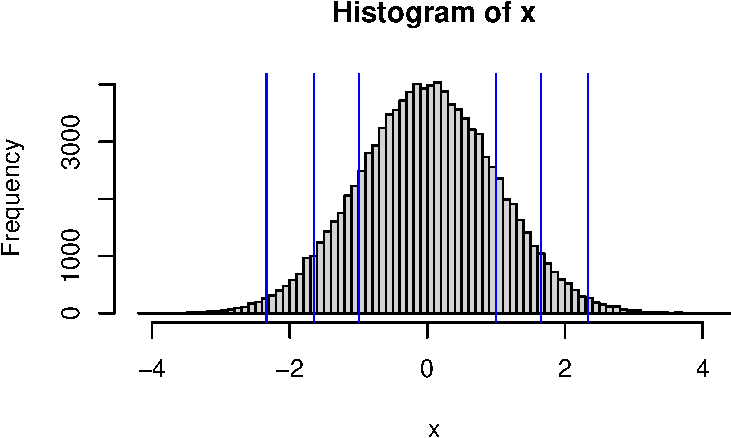
\includegraphics{032_univariate_files/figure-pdf/unnamed-chunk-17-1.pdf}

\subsection{Inter-quartile range (IQR)}\label{inter-quartile-range-iqr}

It is simply the difference between the 3rd and the 1st quartiles:
\[IQR = Q3(x) - Q1(x)\].

Again for the variable \emph{Age}, it equals: \(27.75 - 25.25 = 2.5\)

\begin{Shaded}
\begin{Highlighting}[]
\FunctionTok{quantile}\NormalTok{(Age, }\AttributeTok{probs =} \FloatTok{0.75}\NormalTok{) }\SpecialCharTok{{-}} \FunctionTok{quantile}\NormalTok{(Age, }\AttributeTok{probs =} \FloatTok{0.25}\NormalTok{)}
\CommentTok{\#\textgreater{} 75\% }
\CommentTok{\#\textgreater{} 2.5}

\CommentTok{\#or}
\FunctionTok{IQR}\NormalTok{(Age)}
\CommentTok{\#\textgreater{} [1] 2.5}
\end{Highlighting}
\end{Shaded}

\subsection{Variance and Standard
Deviation}\label{variance-and-standard-deviation}

Although quantiles and plots are very much in use to describe the spread
of a distribution, statistical analysis relies most heavily on the
notion of variance.

First, think about the simplest way you can measure how a given
observation is far from, (i.e.~spread out of) a general expected value.
A pretty effective way is to measure the difference between that
observation and the mean of observations.

The Deviation to the mean for an individual i is \[v_i=x_i-\bar{x}\]

It is then very tempting to say that the general dispersion of a
variable is simply the sum of all those values. In order for the number
not to grow with the number of observations, we then compute an average
deviation by dividing by \(n\)

\[\Sigma_i(x_i-\bar{x})/n\]

But is this a good idea?

Take the Age example:

\begin{Shaded}
\begin{Highlighting}[]
\NormalTok{v}\OtherTok{\textless{}{-}}\NormalTok{ Age}\SpecialCharTok{{-}}\FunctionTok{mean}\NormalTok{(Age) }\CommentTok{\#set of deviations to the mean}
\FunctionTok{sum}\NormalTok{(v)}\SpecialCharTok{/}\FunctionTok{length}\NormalTok{(v)}
\CommentTok{\#\textgreater{} [1] 0}
\end{Highlighting}
\end{Shaded}

It seems there is no ``spreading'' ? In fact, all the negative
deviations compensate (here exactly) the positive deviations.

We can rather remove the signs and use the absolute value of each
deviation, sum them up and divide by \(n\).

This is called MAD, the \textbf{Mean Absolute Deviation} and is quite
easy to interpret indeed.

\begin{Shaded}
\begin{Highlighting}[]
\NormalTok{abs\_v}\OtherTok{\textless{}{-}} \FunctionTok{abs}\NormalTok{(Age}\SpecialCharTok{{-}}\FunctionTok{mean}\NormalTok{(Age)) }\CommentTok{\#set of deviations to the mean}
\FunctionTok{mean}\NormalTok{(abs\_v)}
\CommentTok{\#\textgreater{} [1] 4.8}
\end{Highlighting}
\end{Shaded}

Yet, one could argue that large deviations to the mean are more
important than the smaller ones to describe the pattern of deviations,
especially since in a normal population there are more values closer to
the mean than farther.

Rather than using absolute deviations, (most of) statisticians have
therefore opted for squaring the deviations, which is still symmetrical
and has the same characteristic of turning every negative value into a
positive one.

We therefore usually consider the sum of squared deviations to the mean:

\[\Sigma_i^n(x_i-\bar{x})^2\] which, we then divide by the number of
observations to avoid the value to grow with the number of observations,
thus allowing comparisons. It is then called the \textbf{variance}. More
precisely, if we use a sample, we still need to use one of our
observation in order to estimate the mean, hence we are left with
\(n-1\) degrees of freedom.

The empirical variance is then given by:

\[var_x = s^2_x = \dfrac{1}{n-1} \sum_{i=1}^n (x_i-\bar{x})^2\]

and the theoretical variance:

\[var_X = \sigma^2_X = \dfrac{1}{N} \sum_{i=1}^N (X_i-E(X))^2\]
\[= E(X-E(X))^2 = E(X-\mu)^2 \]

where \(E(X)\) is the expected mean of the population (or
``Esperance'').

The variance is thus a single number that gives insight on how the
variable is spread around the mean value. A small value (close to 0)
indicates a small variability: values are not very different from the
mean value. A high value indicated a strong variability.

The variance cannot be negative.

In R, we use the \texttt{var()} functio, which we here first
reconstruct:

\begin{Shaded}
\begin{Highlighting}[]
\NormalTok{(Age}\SpecialCharTok{{-}}\FunctionTok{mean}\NormalTok{(Age))}\SpecialCharTok{\^{}}\DecValTok{2} \CommentTok{\#squared deviations to the mean}
\CommentTok{\#\textgreater{}  [1]  16   4   1  36 529   4   4   9  16   1}
\FunctionTok{sum}\NormalTok{((Age}\SpecialCharTok{{-}}\FunctionTok{mean}\NormalTok{(Age))}\SpecialCharTok{\^{}}\DecValTok{2}\NormalTok{) }\CommentTok{\#sum of squared deviations to the mean}
\CommentTok{\#\textgreater{} [1] 620}
\FunctionTok{sum}\NormalTok{((Age}\SpecialCharTok{{-}}\FunctionTok{mean}\NormalTok{(Age))}\SpecialCharTok{\^{}}\DecValTok{2}\NormalTok{)}\SpecialCharTok{/}\NormalTok{(}\FunctionTok{length}\NormalTok{(Age)}\SpecialCharTok{{-}}\DecValTok{1}\NormalTok{) }\CommentTok{\#...divided by n{-}1}
\CommentTok{\#\textgreater{} [1] 68.88889}

\FunctionTok{var}\NormalTok{(Age)}
\CommentTok{\#\textgreater{} [1] 68.88889}
\FunctionTok{var}\NormalTok{(Age2)}
\CommentTok{\#\textgreater{} [1] 4.027778}
\end{Highlighting}
\end{Shaded}

We see that the default in R for \texttt{var()} is to divide by \(n-1\),
i.e.~the sample variance.

Finally, we like the ``dispersion'' to be expressed in the same units as
the original variable, i.e.~years in this case. It is already the case
for the Mean Absolute Deviation. We need to take the square root of the
variance to obtain a ``standard deviation'':

The standard deviations corresponding to the sample and population
variance are then given by:

\[s_x = \sqrt{\dfrac{1}{n-1} \sum_{i=1}^n (x_i-\bar{x})^2}\]

\[\sigma_X = \sqrt{\dfrac{1}{N} \sum_{i=1}^N (X_i-E(X))^2}\]

And can be computed using:

\begin{Shaded}
\begin{Highlighting}[]
\FunctionTok{sqrt}\NormalTok{(}\FunctionTok{var}\NormalTok{(Age))}
\CommentTok{\#\textgreater{} [1] 8.299933}
\FunctionTok{sqrt}\NormalTok{(}\FunctionTok{var}\NormalTok{(Age2))}
\CommentTok{\#\textgreater{} [1] 2.006932}
\CommentTok{\#or simply}
\FunctionTok{sd}\NormalTok{(Age) }\CommentTok{\#again remember it is the sample sd}
\CommentTok{\#\textgreater{} [1] 8.299933}
\FunctionTok{sd}\NormalTok{(Age2)}
\CommentTok{\#\textgreater{} [1] 2.006932}
\end{Highlighting}
\end{Shaded}

\section{Visualize a distribution}\label{visualize-a-distribution}

Visualizing a distribution with graphics is important for both
supporting the analysis and dissemination.

We have seen some graphics already above and we are going to produce
improved graphics with ggplot later on. Without spending much time on
design, the purpose here is show how graphics accompany the univariate
statistics we introduced.

\subsection{Boxplots}\label{boxplots}

A boxplot visually provides a number of information about the
distribution of a variable

\begin{itemize}
\tightlist
\item
  the median value (thick black line),
\item
  the inter-quartile range (IQR) (the black box),
\item
  the minimum and maximum values or 1.5 times the IQR (horizontal
  lines),
\item
  the outlier(s) (dots out of the whiskers).
\end{itemize}

Values are considered outliers when they fall outside the whiskers, that
is outside a distance of 1.5 times the IQR. In absence of such outliers
the horizontal lines show the extrema (min and max).

We have added the mean as a red point to clarify here the difference
between the mean and median.

Examine the difference again between Age and Age2

\begin{Shaded}
\begin{Highlighting}[]
\FunctionTok{par}\NormalTok{ (}\AttributeTok{mfrow =} \FunctionTok{c}\NormalTok{(}\DecValTok{1}\NormalTok{, }\DecValTok{2}\NormalTok{)) }\CommentTok{\# to display multiple plots at once}
\FunctionTok{boxplot}\NormalTok{(Age, }\AttributeTok{ylab =} \StringTok{"Age"}\NormalTok{, }\AttributeTok{main =} \StringTok{"Boxplot of Age"}\NormalTok{)}
\FunctionTok{points}\NormalTok{(}\FunctionTok{mean}\NormalTok{(Age), }\AttributeTok{col =} \DecValTok{2}\NormalTok{, }\AttributeTok{pch =} \DecValTok{18}\NormalTok{)}

\FunctionTok{boxplot}\NormalTok{(Age2, }\AttributeTok{ylab =} \StringTok{"Age2"}\NormalTok{, }\AttributeTok{main =} \StringTok{"Boxplot of Age2"}\NormalTok{)}
\FunctionTok{points}\NormalTok{(}\FunctionTok{mean}\NormalTok{(Age2), }\AttributeTok{col =} \DecValTok{2}\NormalTok{, }\AttributeTok{pch =} \DecValTok{18}\NormalTok{)}
\end{Highlighting}
\end{Shaded}

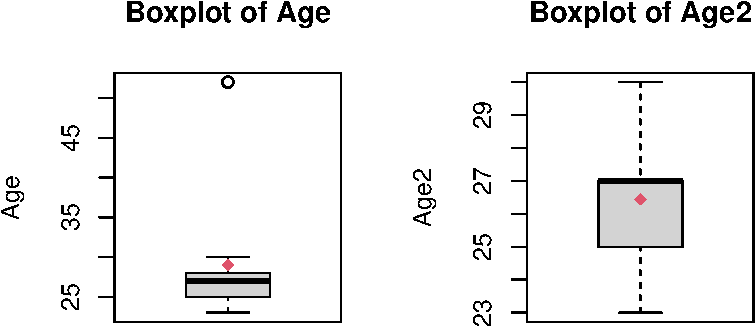
\includegraphics{032_univariate_files/figure-pdf/unnamed-chunk-23-1.pdf}

\subsection{Stem and leaf}\label{stem-and-leaf}

Probably less in use nowadayd for visual purpose and reporting, a stem
and leaf graph is a very effective way to look into the distribution of
a variable while you are exploring, analyzing your data in the console.

It is not actually a plot but a presentation of the values into a
``stem'', which is made of the values that are present across all cases
and then a ``leaf'' where the remaining parts of each numbers is shown
and concatenated, thus showing a kind of frequency together with the
values:

Examine the case for Age and Age2:

\begin{Shaded}
\begin{Highlighting}[]
\FunctionTok{stem}\NormalTok{(Age)}
\CommentTok{\#\textgreater{} }
\CommentTok{\#\textgreater{}   The decimal point is 1 digit(s) to the right of the |}
\CommentTok{\#\textgreater{} }
\CommentTok{\#\textgreater{}   2 | 35567778}
\CommentTok{\#\textgreater{}   3 | 0}
\CommentTok{\#\textgreater{}   4 | }
\CommentTok{\#\textgreater{}   5 | 2}
\FunctionTok{stem}\NormalTok{(Age2)}
\CommentTok{\#\textgreater{} }
\CommentTok{\#\textgreater{}   The decimal point is at the |}
\CommentTok{\#\textgreater{} }
\CommentTok{\#\textgreater{}   22 | 0}
\CommentTok{\#\textgreater{}   24 | 00}
\CommentTok{\#\textgreater{}   26 | 0000}
\CommentTok{\#\textgreater{}   28 | 0}
\CommentTok{\#\textgreater{}   30 | 0}
\end{Highlighting}
\end{Shaded}

\subsection{Histogram}\label{histogram}

Histograms are probably the first go to graphic in order to visualize a
distribution

Let's reuse the x normal variable we created earlier and plot both its
boxplot and the histogram

\begin{Shaded}
\begin{Highlighting}[]
\FunctionTok{set.seed}\NormalTok{(}\DecValTok{233}\NormalTok{)}
\NormalTok{x}\OtherTok{\textless{}{-}}\FunctionTok{rnorm}\NormalTok{(}\AttributeTok{n =} \DecValTok{100000}\NormalTok{, }\AttributeTok{mean=}\DecValTok{0}\NormalTok{, }\AttributeTok{sd=}\DecValTok{1}\NormalTok{)}

\FunctionTok{summary}\NormalTok{(x)}
\CommentTok{\#\textgreater{}      Min.   1st Qu.    Median      Mean   3rd Qu.      Max. }
\CommentTok{\#\textgreater{} {-}4.127442 {-}0.668690  0.004522  0.003651  0.682818  4.323841}
\FunctionTok{boxplot}\NormalTok{(x, }\AttributeTok{main =} \StringTok{"Boxplot of a random variable following N(0,1) with n = 100,000"}\NormalTok{)}
\end{Highlighting}
\end{Shaded}

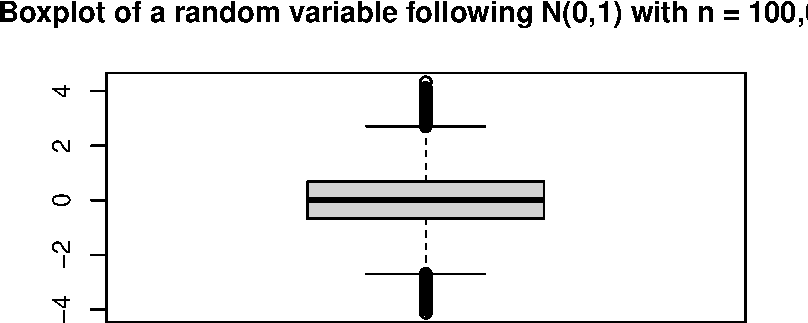
\includegraphics{032_univariate_files/figure-pdf/unnamed-chunk-25-1.pdf}

\begin{Shaded}
\begin{Highlighting}[]
\FunctionTok{hist}\NormalTok{(x)}
\end{Highlighting}
\end{Shaded}

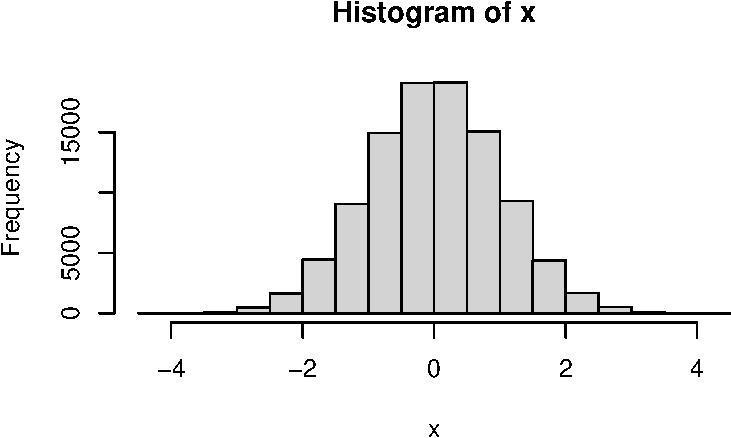
\includegraphics{032_univariate_files/figure-pdf/unnamed-chunk-25-2.pdf}

A histogram is more detailed than a boxplot because it shows every data
but does not provide a central or dispersion measure. Key to using a
histogram is to play with the number of bars, otherwise some
information, gaps, or multimodalities may be not be seen. You adapt the
number of bars using the option ``breaks''

\begin{Shaded}
\begin{Highlighting}[]
\FunctionTok{par}\NormalTok{(}\AttributeTok{mfrow=}\FunctionTok{c}\NormalTok{(}\DecValTok{1}\NormalTok{,}\DecValTok{2}\NormalTok{))}
\FunctionTok{hist}\NormalTok{(x, }\AttributeTok{breaks=}\DecValTok{5}\NormalTok{)}
\FunctionTok{hist}\NormalTok{(x, }\AttributeTok{breaks=}\DecValTok{100}\NormalTok{)}
\end{Highlighting}
\end{Shaded}

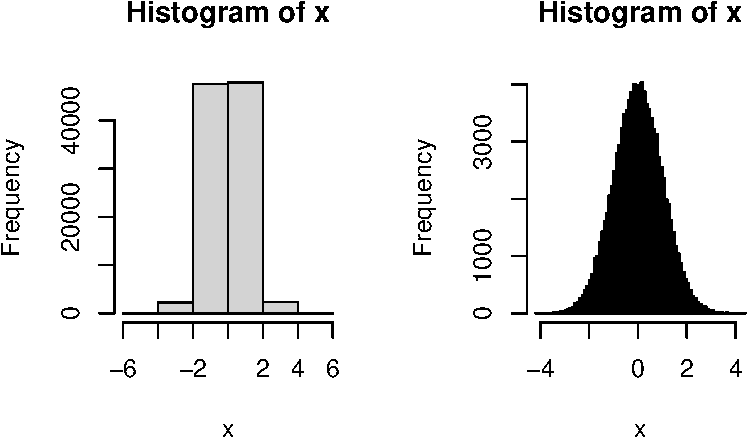
\includegraphics{032_univariate_files/figure-pdf/unnamed-chunk-26-1.pdf}

For a categorical variable (factor), the function \texttt{plot()} gives
the counts of each category (level). We have worked an example using Le
Tour de France data earlier in the course. It is similar to a
visualisation of the \texttt{table()} output and is equivalent to the
function \texttt{hist()} for quantitative variables.

\begin{Shaded}
\begin{Highlighting}[]
\FunctionTok{table}\NormalTok{(score)}
\CommentTok{\#\textgreater{} score}
\CommentTok{\#\textgreater{} A B C }
\CommentTok{\#\textgreater{} 3 3 4}
\FunctionTok{plot}\NormalTok{(score, }\AttributeTok{main =} \StringTok{"Scores"}\NormalTok{, }\AttributeTok{ylab =} \StringTok{"Frequency"}\NormalTok{)}
\end{Highlighting}
\end{Shaded}

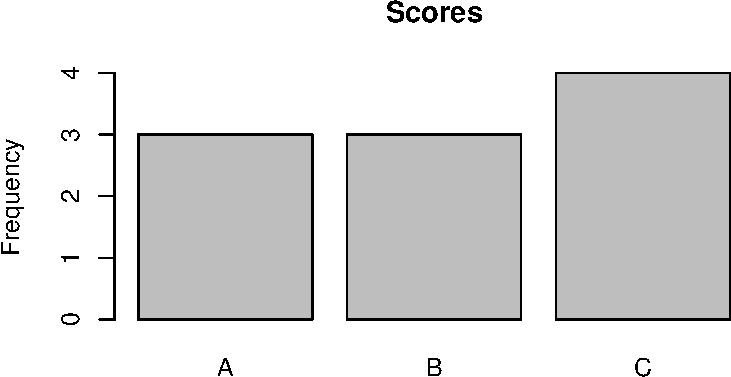
\includegraphics{032_univariate_files/figure-pdf/unnamed-chunk-27-1.pdf}

For a numeric variable, a call to plot, shows values along the vertical
axis and the index of the rows along the horizontal axis, which is
rarely a useful information.

\begin{Shaded}
\begin{Highlighting}[]
\FunctionTok{plot}\NormalTok{(x)}
\end{Highlighting}
\end{Shaded}

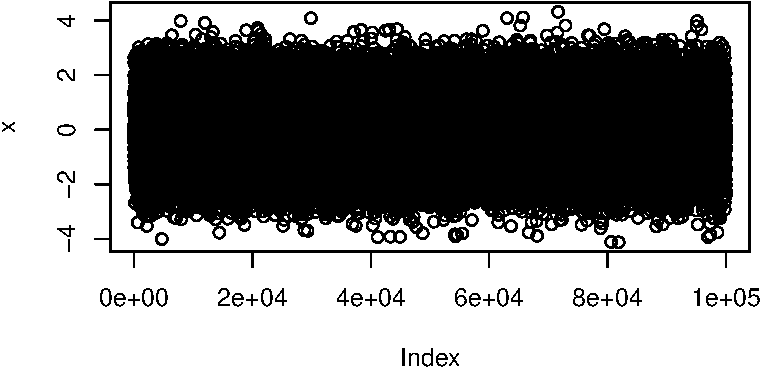
\includegraphics{032_univariate_files/figure-pdf/unnamed-chunk-28-1.pdf}

\section{The shape of distributions: Skewness and
Kurtosis}\label{the-shape-of-distributions-skewness-and-kurtosis}

\subsection{First and second moments:}\label{first-and-second-moments}

We have seen earlier that the very first way to characterise a
distribution is to use its mean and that the second way is to use the
variance (or the square root of the variance, i.e.~the standard
deviation).

The mean and the variance are also named, respectively, the first and
second moment of a distribution

Indeed, for discrete data, the \textbf{mean} (or expectation) is
calculated as:

\[\mu = E[X] = \sum_{i} x_i p(x_i)\] where \(x_i\) are the values and
\(p(x_i)\) are their probabilities.

Note 1: for continuous variables, we should in fact use an integral
rather that the sum symbol. Note 2, the ``zeroth'' moment of the
distribution is in fact the sum of probabilities (x\_i), i.e.~the total
mass (the concept is borrowed from physics), i.e.~1.

The \textbf{variance} is the second order moment, measuring the spread
of the distribution around the mean. We have seen it is defined in
difference to the mean with a square exponent:

\[\sigma^2 = E[(X - \mu)^2] = \sum_{i} (x_i - \mu)^2 p(x_i)\] We can
actually go on with higher exponents and use higher level moments to
describe the shape of a distribution.

\subsection{Third moment: Skewness}\label{third-moment-skewness}

The skewness is the third order moment of a distribution. The
\textbf{skewness measures the asymmetry of the distribution around the
mean}. It is is calculated as:

\[\gamma_1 = E\left[\left(\frac{X - \mu}{\sigma}\right)^3\right] = \sum_{i} \left(\frac{x_i - \mu}{\sigma}\right)^3 p(x_i)\]

In addition to the cubic exponent applied to the deviation to the mean,
you notice we also divide by the standard deviation \(\sigma\) to make
the measure dimensionless, i.e.~comparable across cases with different
units. The skewness is not influenced by the scale of the data.

In practice, the skewness is computed as follows:

\[\dfrac {\sum_{i=1}^{n} (x_i - \bar{x})^3} {n s^3}\]

\begin{Shaded}
\begin{Highlighting}[]
\FunctionTok{set.seed}\NormalTok{(}\DecValTok{101}\NormalTok{)}
\NormalTok{x}\OtherTok{\textless{}{-}}\FunctionTok{rnorm}\NormalTok{(}\DecValTok{1000}\NormalTok{, }\AttributeTok{mean=}\DecValTok{50}\NormalTok{,}\AttributeTok{sd=}\DecValTok{5}\NormalTok{)}
\FunctionTok{mean}\NormalTok{(x)}
\CommentTok{\#\textgreater{} [1] 49.82569}
\FunctionTok{median}\NormalTok{(x)}
\CommentTok{\#\textgreater{} [1] 49.72804}
\NormalTok{e1071}\SpecialCharTok{::}\FunctionTok{skewness}\NormalTok{(x)}
\CommentTok{\#\textgreater{} [1] {-}0.004246246}
\NormalTok{e1071}\SpecialCharTok{::}\FunctionTok{skewness}\NormalTok{((x}\DecValTok{{-}100}\NormalTok{)}\SpecialCharTok{/}\DecValTok{1000}\NormalTok{) }\CommentTok{\#with this you see it is not influenced by any rescaling}
\CommentTok{\#\textgreater{} [1] {-}0.004246246}
\FunctionTok{sum}\NormalTok{((x}\SpecialCharTok{{-}}\FunctionTok{mean}\NormalTok{(x))}\SpecialCharTok{\^{}}\DecValTok{3}\NormalTok{)}\SpecialCharTok{/}\NormalTok{(}\FunctionTok{sd}\NormalTok{(x)}\SpecialCharTok{\^{}}\DecValTok{3}\SpecialCharTok{*}\FunctionTok{length}\NormalTok{(x)) }\CommentTok{\#manual computation}
\CommentTok{\#\textgreater{} [1] {-}0.004246246}
\end{Highlighting}
\end{Shaded}

When the skewness is \(>0\), the tail of the distribution is heavier on
the right side. This means there are more extreme values on the higher
end. The mean is greater than the median.

When the skewness is \(<0\), the tail of the distribution is heavier on
the left side. This means there are more extreme values on the lower
end. The mean is lower than the median.

A value around zero indicates a symmetric distribution.

\begin{Shaded}
\begin{Highlighting}[]
\FunctionTok{set.seed}\NormalTok{(}\DecValTok{101}\NormalTok{)}
\NormalTok{right\_skewed }\OtherTok{\textless{}{-}}\NormalTok{ x }\SpecialCharTok{+} \FunctionTok{rexp}\NormalTok{(}\DecValTok{1000}\NormalTok{, }\AttributeTok{rate =} \FloatTok{0.1}\NormalTok{) }\CommentTok{\#we add an exp to the previous x for generating a right skewed distribution}
\NormalTok{left\_skewed }\OtherTok{\textless{}{-}} \FunctionTok{rnorm}\NormalTok{(}\DecValTok{1000}\NormalTok{, }\AttributeTok{mean =} \DecValTok{50}\NormalTok{, }\AttributeTok{sd =} \DecValTok{5}\NormalTok{) }\SpecialCharTok{{-}} \FunctionTok{rexp}\NormalTok{(}\DecValTok{100}\NormalTok{, }\AttributeTok{rate =} \FloatTok{0.1}\NormalTok{) }\CommentTok{\#left skewed}

\FunctionTok{hist}\NormalTok{(x, }\AttributeTok{main =} \StringTok{"Symmetric"}\NormalTok{, }\AttributeTok{col =} \StringTok{"blue"}\NormalTok{, }\AttributeTok{breaks =} \DecValTok{20}\NormalTok{)}
\end{Highlighting}
\end{Shaded}

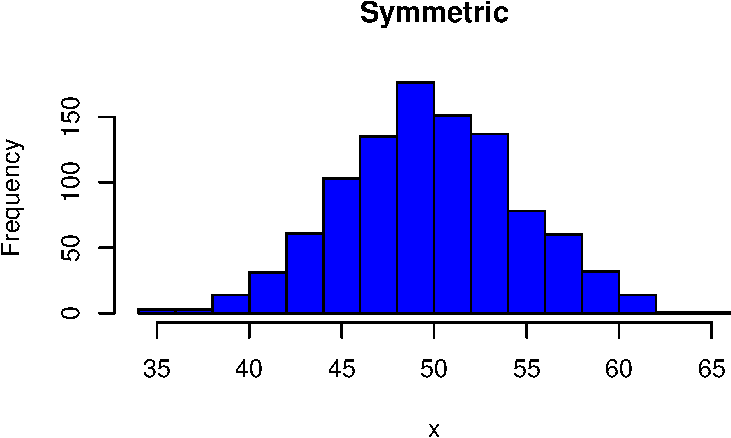
\includegraphics{032_univariate_files/figure-pdf/unnamed-chunk-30-1.pdf}

\begin{Shaded}
\begin{Highlighting}[]
\FunctionTok{hist}\NormalTok{(right\_skewed, }\AttributeTok{main =} \StringTok{"Right{-}skewed"}\NormalTok{,}\AttributeTok{col =} \StringTok{"green"}\NormalTok{, }\AttributeTok{breaks =} \DecValTok{20}\NormalTok{)}
\end{Highlighting}
\end{Shaded}

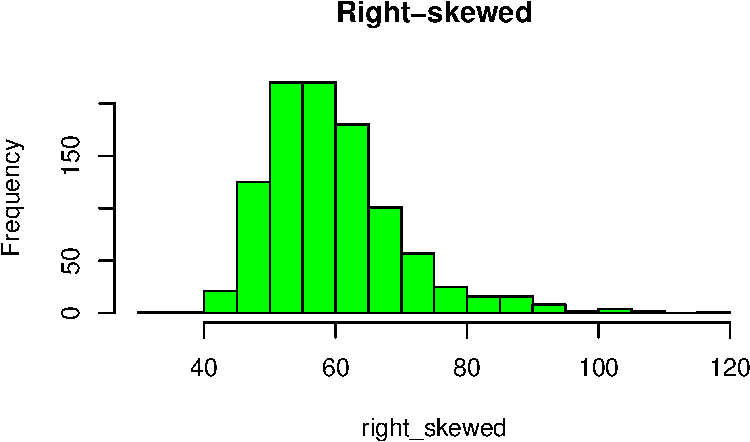
\includegraphics{032_univariate_files/figure-pdf/unnamed-chunk-30-2.pdf}

\begin{Shaded}
\begin{Highlighting}[]
\FunctionTok{hist}\NormalTok{(left\_skewed, }\AttributeTok{main =} \StringTok{"Left{-}skewed"}\NormalTok{, }\AttributeTok{col =} \StringTok{"red"}\NormalTok{, }\AttributeTok{breaks =} \DecValTok{20}\NormalTok{)}
\end{Highlighting}
\end{Shaded}

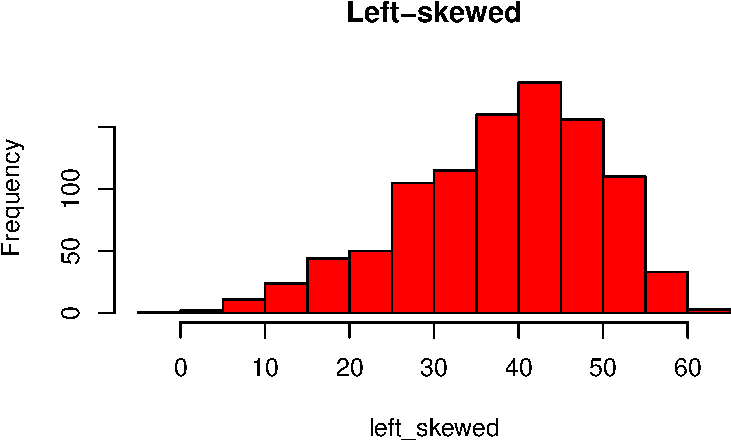
\includegraphics{032_univariate_files/figure-pdf/unnamed-chunk-30-3.pdf}

\begin{Shaded}
\begin{Highlighting}[]

\NormalTok{e1071}\SpecialCharTok{::}\FunctionTok{skewness}\NormalTok{(x)}
\CommentTok{\#\textgreater{} [1] {-}0.004246246}
\NormalTok{e1071}\SpecialCharTok{::}\FunctionTok{skewness}\NormalTok{(right\_skewed)}
\CommentTok{\#\textgreater{} [1] 1.350504}
\NormalTok{e1071}\SpecialCharTok{::}\FunctionTok{skewness}\NormalTok{(left\_skewed)}
\CommentTok{\#\textgreater{} [1] {-}0.5836373}
\end{Highlighting}
\end{Shaded}

\subsection{Fourth moment: Kurtosis}\label{fourth-moment-kurtosis}

The Kurtosis is the fourth order moment of a distribution. The
\textbf{Kurtosis measures the peakness of the distribution} and is
calculated as:

\[\gamma_2 = E\left[\left(\frac{X - \mu}{\sigma}\right)^4\right] - 3 = \sum_{i} \left(\frac{x_i - \mu}{\sigma}\right)^4 p(x_i) - 3\]

You notice the exponent to the level 4 applied to the deviations to the
mean and that similarly to the skewness, we also divide by the standard
deviation \(\sigma\) to make the measure dimensionless, i.e.~comparable
across cases with different units. The Kurtosis is not influenced by the
scale of the data.

In practice in R, the Kurtosis is similar to the skewness described
above:

\[\dfrac {\sum_{i=1}^{n} (x_i - \bar{x})^4} {n s^4}\] However it is
adjusted with some correction for small sample sizes and for comparison
to a normal distribution for which the result would be 3. See the help
for how it is computed by default

\begin{Shaded}
\begin{Highlighting}[]
\FunctionTok{set.seed}\NormalTok{(}\DecValTok{101}\NormalTok{)}
\NormalTok{x}\OtherTok{\textless{}{-}}\FunctionTok{rnorm}\NormalTok{(}\DecValTok{1000}\NormalTok{, }\AttributeTok{mean=}\DecValTok{50}\NormalTok{,}\AttributeTok{sd=}\DecValTok{5}\NormalTok{)}
\NormalTok{e1071}\SpecialCharTok{::}\FunctionTok{kurtosis}\NormalTok{(x)}
\CommentTok{\#\textgreater{} [1] {-}0.119472}
\NormalTok{e1071}\SpecialCharTok{::}\FunctionTok{kurtosis}\NormalTok{((x}\DecValTok{{-}100}\NormalTok{)}\SpecialCharTok{/}\DecValTok{1000}\NormalTok{) }\CommentTok{\#with this you see it is not dependent on scale }
\CommentTok{\#\textgreater{} [1] {-}0.119472}
\end{Highlighting}
\end{Shaded}

Using this implementation, a Kurtosis close to 0 then indicates a
distribution similar in shape to a normal (bell-shaped) distribution. A
\textbf{positive kurtosis indicates a more peaked} distribution, also
named \textbf{leptokurtic}.

A \textbf{negative kurtosis} indicates a \textbf{less peaked} shape,
named \textbf{platykurtic}.

as an example, we can add some extreme values to the normal values we
created earlier in order to higher peak look or trim the extremes of a
normal distribution to have a flatter one:

\begin{Shaded}
\begin{Highlighting}[]
\FunctionTok{set.seed}\NormalTok{(}\DecValTok{1010}\NormalTok{)}
\NormalTok{x}\OtherTok{\textless{}{-}}\FunctionTok{rnorm}\NormalTok{(}\DecValTok{1000}\NormalTok{, }\AttributeTok{mean=}\DecValTok{50}\NormalTok{,}\AttributeTok{sd=}\DecValTok{5}\NormalTok{)}
\NormalTok{x\_peaker}\OtherTok{\textless{}{-}}\FunctionTok{c}\NormalTok{(x, }\FunctionTok{rnorm}\NormalTok{(}\DecValTok{300}\NormalTok{, }\AttributeTok{mean =} \DecValTok{50}\NormalTok{, }\AttributeTok{sd =} \DecValTok{20}\NormalTok{))}
\NormalTok{x\_flatter}\OtherTok{\textless{}{-}}\NormalTok{x[}\FunctionTok{abs}\NormalTok{(x) }\SpecialCharTok{\textless{}} \DecValTok{60}\NormalTok{]}

\FunctionTok{hist}\NormalTok{(x, }\AttributeTok{main =} \StringTok{"Normal"}\NormalTok{, }\AttributeTok{col =} \StringTok{"blue"}\NormalTok{, }\AttributeTok{breaks =} \DecValTok{20}\NormalTok{)}
\end{Highlighting}
\end{Shaded}

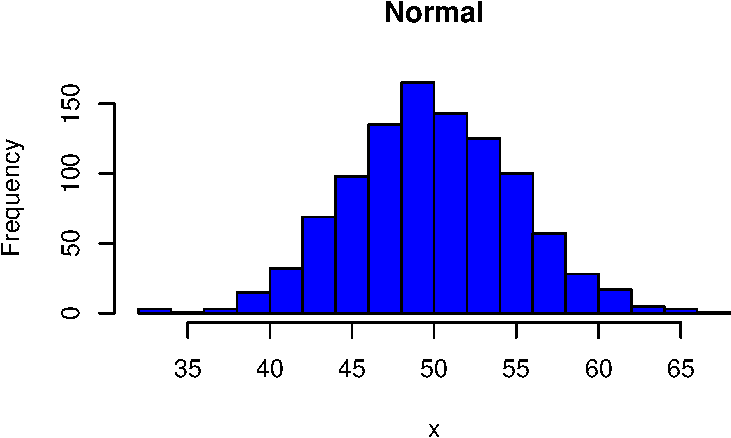
\includegraphics{032_univariate_files/figure-pdf/unnamed-chunk-32-1.pdf}

\begin{Shaded}
\begin{Highlighting}[]
\FunctionTok{hist}\NormalTok{(x\_peaker, }\AttributeTok{main =} \StringTok{"Higher peak"}\NormalTok{,}\AttributeTok{col =} \StringTok{"green"}\NormalTok{, }\AttributeTok{breaks =} \DecValTok{20}\NormalTok{)}
\end{Highlighting}
\end{Shaded}

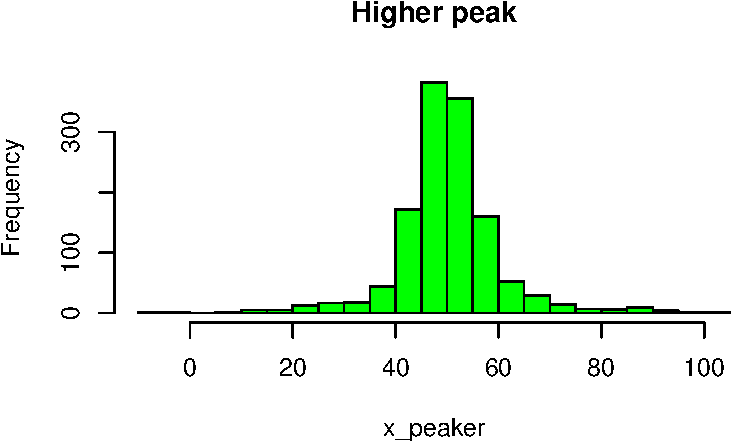
\includegraphics{032_univariate_files/figure-pdf/unnamed-chunk-32-2.pdf}

\begin{Shaded}
\begin{Highlighting}[]
\FunctionTok{hist}\NormalTok{(x\_flatter, }\AttributeTok{main =} \StringTok{"Flatter"}\NormalTok{, }\AttributeTok{col =} \StringTok{"red"}\NormalTok{, }\AttributeTok{breaks =} \DecValTok{20}\NormalTok{)}
\end{Highlighting}
\end{Shaded}

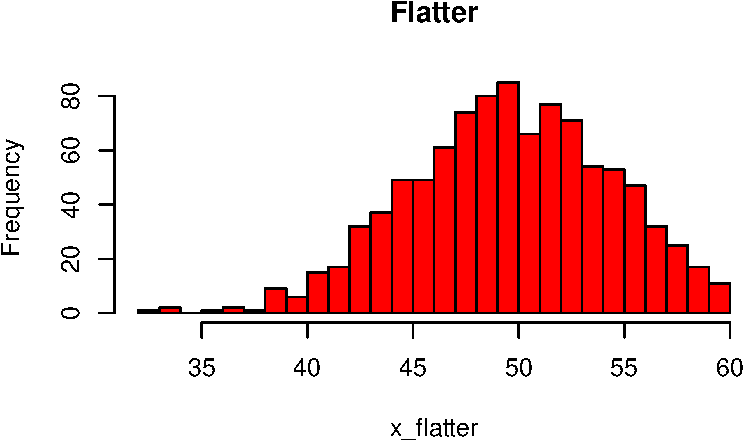
\includegraphics{032_univariate_files/figure-pdf/unnamed-chunk-32-3.pdf}

\begin{Shaded}
\begin{Highlighting}[]

\NormalTok{e1071}\SpecialCharTok{::}\FunctionTok{kurtosis}\NormalTok{(x)}
\CommentTok{\#\textgreater{} [1] 0.07423458}
\NormalTok{e1071}\SpecialCharTok{::}\FunctionTok{kurtosis}\NormalTok{(x\_peaker)}
\CommentTok{\#\textgreater{} [1] 5.789643}
\NormalTok{e1071}\SpecialCharTok{::}\FunctionTok{kurtosis}\NormalTok{(x\_flatter)}
\CommentTok{\#\textgreater{} [1] {-}0.1829135}
\end{Highlighting}
\end{Shaded}

\chapter{Discretisation}\label{sec-discretisation}

Geographers, maybe more than others because they like to produce maps,
are often tempted to cut a numerical vector into a set classes.

A typical use is the cartography of a continuous variable in a set of 5,
6 or 7 groups, knowing the human eye has difficulties to disentangle
more colours. GIS and mapping software all have a menu where
``discretisation'' is made using a number of manually defined limits of
preset algorithms, such as ``Natural breaks'', ``quantiles'', etc.

In R, the function \texttt{cut()}` is the base function to divide a
range of numeric values x into intervals by a number of break values. It
outputs a new factor where each value x is given a level according to
which interval they fall in. The breaks are either

\begin{itemize}
\item
  a scalar greater or equal to 2 for the range to be cut into equal
  length pieces.
\item
  a set of breaks to be used as the upper and lower limits of each
  discrete category
\end{itemize}

\begin{Shaded}
\begin{Highlighting}[]
\FunctionTok{set.seed}\NormalTok{(}\DecValTok{101}\NormalTok{)}
\NormalTok{x}\OtherTok{\textless{}{-}}\FunctionTok{rnorm}\NormalTok{(}\DecValTok{20}\NormalTok{, }\AttributeTok{mean =} \DecValTok{100}\NormalTok{, }\AttributeTok{sd=}\DecValTok{5}\NormalTok{)}
\NormalTok{xf4}\OtherTok{\textless{}{-}}\FunctionTok{cut}\NormalTok{(x, }\AttributeTok{breaks=}\DecValTok{4}\NormalTok{)}
\FunctionTok{head}\NormalTok{(xf4)}
\CommentTok{\#\textgreater{} [1] (94.1,98.4] (98.4,103]  (94.1,98.4] (98.4,103]  (98.4,103]  (103,107]  }
\CommentTok{\#\textgreater{} Levels: (89.7,94.1] (94.1,98.4] (98.4,103] (103,107]}
\FunctionTok{table}\NormalTok{(xf4)}
\CommentTok{\#\textgreater{} xf4}
\CommentTok{\#\textgreater{} (89.7,94.1] (94.1,98.4]  (98.4,103]   (103,107] }
\CommentTok{\#\textgreater{}           2           5           9           4}
\end{Highlighting}
\end{Shaded}

Notice how the label clearly indicates the (default) closing on the
right of each interval

\begin{Shaded}
\begin{Highlighting}[]
\NormalTok{x}\OtherTok{\textless{}{-}}\FunctionTok{rnorm}\NormalTok{(}\DecValTok{20}\NormalTok{, }\AttributeTok{mean =} \DecValTok{100}\NormalTok{, }\AttributeTok{sd=}\DecValTok{5}\NormalTok{)}
\NormalTok{xf6}\OtherTok{\textless{}{-}}\FunctionTok{cut}\NormalTok{(x, }\AttributeTok{breaks=}\FunctionTok{c}\NormalTok{(}\FunctionTok{min}\NormalTok{(x),}\SpecialCharTok{{-}}\DecValTok{90}\NormalTok{,}\DecValTok{95}\NormalTok{,}\DecValTok{100}\NormalTok{,}\DecValTok{105}\NormalTok{,}\DecValTok{110}\NormalTok{, }\FunctionTok{max}\NormalTok{(x)))}
\FunctionTok{head}\NormalTok{(xf6)}
\CommentTok{\#\textgreater{} [1] (95,100]  (100,105] (95,100]  (89.6,95] (100,105] (89.6,95]}
\CommentTok{\#\textgreater{} Levels: ({-}90,89.6] (89.6,95] (95,100] (100,105] (105,106] (106,110]}
\FunctionTok{table}\NormalTok{(xf6)}
\CommentTok{\#\textgreater{} xf6}
\CommentTok{\#\textgreater{} ({-}90,89.6]  (89.6,95]   (95,100]  (100,105]  (105,106]  (106,110] }
\CommentTok{\#\textgreater{}          1          3          4         10          2          0}
\end{Highlighting}
\end{Shaded}

Since we can choose any breaks, it is pretty easy to adapt and use any
discretisation method one would find elsewhere, e.g.~in mapping
packages.

There is a wonderful package, \texttt{classInt}, that does so and where
you can simply choose the discretisation methodology.

Let's explore!\\
\url{https://cran.r-project.org/web/packages/classInt/classInt.pdf}

We refer to the help of the package and specifically the function
\texttt{classIntervals()}to find out about the available methods

\begin{Shaded}
\begin{Highlighting}[]
\NormalTok{x\_quantile\_5}\OtherTok{\textless{}{-}}\NormalTok{classInt}\SpecialCharTok{::}\FunctionTok{classIntervals}\NormalTok{(x, }\AttributeTok{n=}\DecValTok{5}\NormalTok{, }\AttributeTok{style=}\StringTok{"quantile"}\NormalTok{) }\CommentTok{\#Default style}
\NormalTok{x\_quantile\_5}
\CommentTok{\#\textgreater{} style: quantile}
\CommentTok{\#\textgreater{}   one of 3,876 possible partitions of this variable into 5 classes}
\CommentTok{\#\textgreater{} [89.63447,95.69211) [95.69211,100.2653) [100.2653,102.3357) [102.3357,103.8727) }
\CommentTok{\#\textgreater{}                   4                   4                   4                   4 }
\CommentTok{\#\textgreater{} [103.8727,105.9493] }
\CommentTok{\#\textgreater{}                   4}
\end{Highlighting}
\end{Shaded}

The \texttt{classIntervals()} output has its own class and specific
plotting method that works with a given colour palette

\begin{Shaded}
\begin{Highlighting}[]
\FunctionTok{class}\NormalTok{(x\_quantile\_5)}
\CommentTok{\#\textgreater{} [1] "classIntervals"}
\NormalTok{mycolors}\OtherTok{\textless{}{-}}\FunctionTok{c}\NormalTok{(}\StringTok{"darkgreen"}\NormalTok{,}\StringTok{"lightgreen"}\NormalTok{,}\StringTok{"lightyellow"}\NormalTok{, }\StringTok{"orange"}\NormalTok{, }\StringTok{"orangered"}\NormalTok{)}
\FunctionTok{plot}\NormalTok{(x\_quantile\_5, }\AttributeTok{pal=}\NormalTok{mycolors)}
\end{Highlighting}
\end{Shaded}


\includegraphics{033_discretisation_files/figure-pdf/unnamed-chunk-4-1.pdf}

Given the normality of the distribution, and the use of quantiles, the
central class logically needs a smaller range to host the same number of
values.

Below another split based on standard deviations:

\begin{Shaded}
\begin{Highlighting}[]
\FunctionTok{mean}\NormalTok{(x)}
\CommentTok{\#\textgreater{} [1] 99.97489}
\FunctionTok{sd}\NormalTok{(x)}
\CommentTok{\#\textgreater{} [1] 4.865144}
\NormalTok{x\_sd\_5}\OtherTok{\textless{}{-}}\NormalTok{classInt}\SpecialCharTok{::}\FunctionTok{classIntervals}\NormalTok{(x, }\AttributeTok{n=}\DecValTok{5}\NormalTok{, }\AttributeTok{style=}\StringTok{"sd"}\NormalTok{)}
\NormalTok{x\_sd\_5}
\CommentTok{\#\textgreater{} style: sd}
\CommentTok{\#\textgreater{}   one of 50,388 possible partitions of this variable into 8 classes}
\CommentTok{\#\textgreater{}  [87.81203,90.2446)  [90.2446,92.67717) [92.67717,95.10974) [95.10974,97.54231) }
\CommentTok{\#\textgreater{}                   1                   1                   2                   1 }
\CommentTok{\#\textgreater{} [97.54231,99.97489) [99.97489,102.4075)   [102.4075,104.84)   [104.84,107.2726] }
\CommentTok{\#\textgreater{}                   3                   5                   5                   2}
\FunctionTok{plot}\NormalTok{(x\_sd\_5, }\AttributeTok{pal=}\NormalTok{mycolors)}
\end{Highlighting}
\end{Shaded}


\includegraphics{033_discretisation_files/figure-pdf/unnamed-chunk-5-1.pdf}

And with 7 classes using the ``Jenks'' method, similar to the one we
find within Esri ArcGIS:

\begin{Shaded}
\begin{Highlighting}[]
\NormalTok{x\_jenks\_7}\OtherTok{\textless{}{-}}\NormalTok{classInt}\SpecialCharTok{::}\FunctionTok{classIntervals}\NormalTok{(x, }\AttributeTok{n=}\DecValTok{7}\NormalTok{, }\AttributeTok{style=}\StringTok{"jenks"}\NormalTok{)}
\NormalTok{x\_jenks\_7}
\CommentTok{\#\textgreater{} style: jenks}
\CommentTok{\#\textgreater{}   one of 27,132 possible partitions of this variable into 7 classes}
\CommentTok{\#\textgreater{} [89.63447,89.63447] (89.63447,92.94805] (92.94805,96.37813]  (96.37813,99.4034] }
\CommentTok{\#\textgreater{}                   1                   3                   1                   3 }
\CommentTok{\#\textgreater{}  (99.4034,102.4907] (102.4907,104.6017] (104.6017,105.9493] }
\CommentTok{\#\textgreater{}                   6                   4                   2}
\FunctionTok{plot}\NormalTok{(x\_jenks\_7, }\AttributeTok{pal=}\NormalTok{mycolors)}
\end{Highlighting}
\end{Shaded}


\includegraphics{033_discretisation_files/figure-pdf/unnamed-chunk-6-1.pdf}

Notice that, ahead of plotting, \texttt{classInt}` expanded the number
of colours, which we provided. In fact, 2 would be enough:

\begin{Shaded}
\begin{Highlighting}[]
\FunctionTok{plot}\NormalTok{(x\_jenks\_7, }\AttributeTok{pal=}\FunctionTok{c}\NormalTok{(}\StringTok{"yellow"}\NormalTok{,}\StringTok{"red"}\NormalTok{))}
\end{Highlighting}
\end{Shaded}


\includegraphics{033_discretisation_files/figure-pdf/unnamed-chunk-7-1.pdf}

Interestingly, rather that specifying a number of classes, one could
also use the same breaks as a standard boxplot:

\begin{Shaded}
\begin{Highlighting}[]
\NormalTok{x\_box}\OtherTok{\textless{}{-}}\NormalTok{classInt}\SpecialCharTok{::}\FunctionTok{classIntervals}\NormalTok{(x,  }\AttributeTok{style=}\StringTok{"box"}\NormalTok{)}
\NormalTok{x\_box}
\CommentTok{\#\textgreater{} style: box}
\CommentTok{\#\textgreater{}   one of 11,628 possible partitions of this variable into 6 classes}
\CommentTok{\#\textgreater{} [89.63447,89.84276) [89.84276,98.08961) [98.08961,101.8191) [101.8191,103.5875) }
\CommentTok{\#\textgreater{}                   1                   4                   5                   5 }
\CommentTok{\#\textgreater{} [103.5875,111.8343)      [111.8343,Inf] }
\CommentTok{\#\textgreater{}                   5                   0}
\FunctionTok{quantile}\NormalTok{(x,}\AttributeTok{probs=}\FunctionTok{c}\NormalTok{(}\FloatTok{0.25}\NormalTok{,}\FloatTok{0.5}\NormalTok{,}\FloatTok{0.75}\NormalTok{))}
\CommentTok{\#\textgreater{}       25\%       50\%       75\% }
\CommentTok{\#\textgreater{}  98.08961 101.81905 103.58750}
\FunctionTok{c}\NormalTok{(}\FunctionTok{quantile}\NormalTok{(x,}\AttributeTok{probs=}\FloatTok{0.25}\NormalTok{)}\SpecialCharTok{{-}}\FloatTok{1.5}\SpecialCharTok{*}\FunctionTok{IQR}\NormalTok{(x),}
  \FunctionTok{quantile}\NormalTok{(x,}\AttributeTok{probs=}\FloatTok{0.75}\NormalTok{)}\SpecialCharTok{+}\FloatTok{1.5}\SpecialCharTok{*}\FunctionTok{IQR}\NormalTok{(x))}
\CommentTok{\#\textgreater{}       25\%       75\% }
\CommentTok{\#\textgreater{}  89.84276 111.83435}
\FunctionTok{plot}\NormalTok{(x\_box, }\AttributeTok{pal=}\NormalTok{mycolors)}
\end{Highlighting}
\end{Shaded}


\includegraphics{033_discretisation_files/figure-pdf/unnamed-chunk-8-1.pdf}

One then retrieves a vector of the categories in which each values fall
using \texttt{findCols()}, which we can easily add to a dataframe as a
new column, or even a vector of colours for use anywhere else using
\texttt{findColours()}.

This is shown below with our Jenks example:

\begin{Shaded}
\begin{Highlighting}[]
\NormalTok{classInt}\SpecialCharTok{::}\FunctionTok{findCols}\NormalTok{(x\_jenks\_7)}
\CommentTok{\#\textgreater{}  [1] 4 6 4 2 6 2 5 4 5 5 6 5 7 1 7 3 5 6 2 5}
\NormalTok{classInt}\SpecialCharTok{::}\FunctionTok{findColours}\NormalTok{(x\_jenks\_7, }\AttributeTok{pal=}\FunctionTok{c}\NormalTok{(}\StringTok{"yellow"}\NormalTok{,}\StringTok{"red"}\NormalTok{))}
\CommentTok{\#\textgreater{}  [1] "\#FF7F00" "\#FF2A00" "\#FF7F00" "\#FFD400" "\#FF2A00" "\#FFD400" "\#FF5500"}
\CommentTok{\#\textgreater{}  [8] "\#FF7F00" "\#FF5500" "\#FF5500" "\#FF2A00" "\#FF5500" "\#FF0000" "\#FFFF00"}
\CommentTok{\#\textgreater{} [15] "\#FF0000" "\#FFAA00" "\#FF5500" "\#FF2A00" "\#FFD400" "\#FF5500"}
\CommentTok{\#\textgreater{} attr(,"palette")}
\CommentTok{\#\textgreater{} [1] "\#FFFF00" "\#FFD400" "\#FFAA00" "\#FF7F00" "\#FF5500" "\#FF2A00" "\#FF0000"}
\CommentTok{\#\textgreater{} attr(,"table")}
\CommentTok{\#\textgreater{} [89.63447,89.63447] (89.63447,92.94805] (92.94805,96.37813]  (96.37813,99.4034] }
\CommentTok{\#\textgreater{}                   1                   3                   1                   3 }
\CommentTok{\#\textgreater{}  (99.4034,102.4907] (102.4907,104.6017] (104.6017,105.9493] }
\CommentTok{\#\textgreater{}                   6                   4                   2}
\end{Highlighting}
\end{Shaded}

Finally,

Finally, you may find more convenient to use
\texttt{classify\_intervals()}, a wrapper for the sequence
\texttt{classIntervals()} and \texttt{findCols()}, in order to issue
directly the factor levels, as in \texttt{cut()}, rather than a more
complex \texttt{classIntervals} object.

\begin{Shaded}
\begin{Highlighting}[]
\NormalTok{k4}\OtherTok{\textless{}{-}}\NormalTok{classInt}\SpecialCharTok{::}\FunctionTok{classify\_intervals}\NormalTok{(x, }\AttributeTok{n=}\DecValTok{4}\NormalTok{, }\AttributeTok{style=}\StringTok{"kmeans"}\NormalTok{)}
\NormalTok{k4}
\CommentTok{\#\textgreater{}  [1] [94.66309,100.1217) [103.0166,105.9493] [94.66309,100.1217)}
\CommentTok{\#\textgreater{}  [4] [89.63447,94.66309) [103.0166,105.9493] [89.63447,94.66309)}
\CommentTok{\#\textgreater{}  [7] [100.1217,103.0166) [94.66309,100.1217) [100.1217,103.0166)}
\CommentTok{\#\textgreater{} [10] [100.1217,103.0166) [103.0166,105.9493] [100.1217,103.0166)}
\CommentTok{\#\textgreater{} [13] [103.0166,105.9493] [89.63447,94.66309) [103.0166,105.9493]}
\CommentTok{\#\textgreater{} [16] [94.66309,100.1217) [100.1217,103.0166) [103.0166,105.9493]}
\CommentTok{\#\textgreater{} [19] [89.63447,94.66309) [100.1217,103.0166)}
\CommentTok{\#\textgreater{} 4 Levels: [89.63447,94.66309) [94.66309,100.1217) ... [103.0166,105.9493]}
\FunctionTok{class}\NormalTok{(k4)}
\CommentTok{\#\textgreater{} [1] "factor"}
\end{Highlighting}
\end{Shaded}

\chapter{Cross-tabulation}\label{sec-cross-tabulation}

There are many instances where a particular variable numeric or factor
is to be computed along or aggregated a categorical variable.

\section{Case of 2 or several factors (contingency
tables)}\label{case-of-2-or-several-factors-contingency-tables}

Suppose a first data.frame is made with a single factor:

\begin{Shaded}
\begin{Highlighting}[]
\NormalTok{D1}\OtherTok{\textless{}{-}}\FunctionTok{data.frame}\NormalTok{(}
\AttributeTok{Score1=}\FunctionTok{factor}\NormalTok{(}\FunctionTok{c}\NormalTok{(}\StringTok{"A"}\NormalTok{,}\StringTok{"A"}\NormalTok{,}\StringTok{"B"}\NormalTok{,}\StringTok{"B"}\NormalTok{,}\StringTok{"C"}\NormalTok{,}\StringTok{"C"}\NormalTok{,}\StringTok{"C"}\NormalTok{,}\StringTok{"C"}\NormalTok{,}\StringTok{"D"}\NormalTok{,}\StringTok{"A"}\NormalTok{,}\StringTok{"A"}\NormalTok{,}\StringTok{"B"}\NormalTok{,}\StringTok{"B"}\NormalTok{,}\StringTok{"C"}\NormalTok{,}\StringTok{"C"}\NormalTok{,}\StringTok{"C"}\NormalTok{,}\StringTok{"C"}\NormalTok{,}\StringTok{"D"}\NormalTok{))}
\NormalTok{)}
\end{Highlighting}
\end{Shaded}

The function \texttt{table()} returns counts, i.e.~frequencies:

\begin{Shaded}
\begin{Highlighting}[]
\FunctionTok{table}\NormalTok{(D1)}
\CommentTok{\#\textgreater{} Score1}
\CommentTok{\#\textgreater{} A B C D }
\CommentTok{\#\textgreater{} 4 4 8 2}
\end{Highlighting}
\end{Shaded}

Let's add a second factor to this data-frame, we see the function table
now returns a cross-tabulation, which we alsso call a contingency table
(and to which we will later add significance tests)

\begin{Shaded}
\begin{Highlighting}[]
\NormalTok{D2}\OtherTok{\textless{}{-}}\NormalTok{D1}
\NormalTok{D2[,}\StringTok{"Gender"}\NormalTok{]}\OtherTok{\textless{}{-}}\FunctionTok{factor}\NormalTok{(}\FunctionTok{c}\NormalTok{(}\StringTok{"M"}\NormalTok{,}\StringTok{"F"}\NormalTok{,}\StringTok{"M"}\NormalTok{,}\StringTok{"F"}\NormalTok{,}\StringTok{"M"}\NormalTok{,}\StringTok{"F"}\NormalTok{,}\StringTok{"M"}\NormalTok{,}\StringTok{"F"}\NormalTok{,}\StringTok{"F"}\NormalTok{,}\StringTok{"F"}\NormalTok{,}\StringTok{"M"}\NormalTok{,}\StringTok{"F"}\NormalTok{,}\StringTok{"M"}\NormalTok{,}\StringTok{"F"}\NormalTok{,}\StringTok{"M"}\NormalTok{,}\StringTok{"F"}\NormalTok{,}\StringTok{"F"}\NormalTok{,}\StringTok{"M"}\NormalTok{))}
\FunctionTok{table}\NormalTok{(D2)}
\CommentTok{\#\textgreater{}       Gender}
\CommentTok{\#\textgreater{} Score1 F M}
\CommentTok{\#\textgreater{}      A 2 2}
\CommentTok{\#\textgreater{}      B 2 2}
\CommentTok{\#\textgreater{}      C 5 3}
\CommentTok{\#\textgreater{}      D 1 1}
\end{Highlighting}
\end{Shaded}

What happens if there are 3 and more factors?

\begin{Shaded}
\begin{Highlighting}[]
\NormalTok{D3}\OtherTok{\textless{}{-}}\NormalTok{D2}
\NormalTok{D3[,}\StringTok{"Score2"}\NormalTok{]}\OtherTok{\textless{}{-}}\FunctionTok{factor}\NormalTok{(}\FunctionTok{c}\NormalTok{(}\StringTok{"B"}\NormalTok{,}\StringTok{"B"}\NormalTok{,}\StringTok{"C"}\NormalTok{,}\StringTok{"C"}\NormalTok{,}\StringTok{"C"}\NormalTok{,}\StringTok{"C"}\NormalTok{,}\StringTok{"D"}\NormalTok{,}\StringTok{"A"}\NormalTok{,}\StringTok{"A"}\NormalTok{,}\StringTok{"B"}\NormalTok{,}\StringTok{"B"}\NormalTok{,}\StringTok{"C"}\NormalTok{,}\StringTok{"C"}\NormalTok{,}\StringTok{"C"}\NormalTok{,}\StringTok{"C"}\NormalTok{,}\StringTok{"D"}\NormalTok{, }\StringTok{"A"}\NormalTok{,}\StringTok{"B"}\NormalTok{))}
\NormalTok{D3[,}\StringTok{"Country"}\NormalTok{]}\OtherTok{=}\FunctionTok{factor}\NormalTok{(}\FunctionTok{c}\NormalTok{(}\StringTok{"LU"}\NormalTok{,}\StringTok{"DE"}\NormalTok{,}\StringTok{"DE"}\NormalTok{,}\StringTok{"DE"}\NormalTok{,}\StringTok{"DE"}\NormalTok{,}\StringTok{"FR"}\NormalTok{,}\StringTok{"DE"}\NormalTok{,}\StringTok{"LU"}\NormalTok{,}\StringTok{"DE"}\NormalTok{,}\StringTok{"BE"}\NormalTok{,}\StringTok{"DE"}\NormalTok{,}\StringTok{"FR"}\NormalTok{,}\StringTok{"BE"}\NormalTok{,}\StringTok{"FR"}\NormalTok{,}\StringTok{"LU"}\NormalTok{,}\StringTok{"LU"}\NormalTok{,}\StringTok{"FR"}\NormalTok{,}\StringTok{"DE"}\NormalTok{))}

\FunctionTok{table}\NormalTok{(D3)}
\CommentTok{\#\textgreater{} , , Score2 = A, Country = BE}
\CommentTok{\#\textgreater{} }
\CommentTok{\#\textgreater{}       Gender}
\CommentTok{\#\textgreater{} Score1 F M}
\CommentTok{\#\textgreater{}      A 0 0}
\CommentTok{\#\textgreater{}      B 0 0}
\CommentTok{\#\textgreater{}      C 0 0}
\CommentTok{\#\textgreater{}      D 0 0}
\CommentTok{\#\textgreater{} }
\CommentTok{\#\textgreater{} , , Score2 = B, Country = BE}
\CommentTok{\#\textgreater{} }
\CommentTok{\#\textgreater{}       Gender}
\CommentTok{\#\textgreater{} Score1 F M}
\CommentTok{\#\textgreater{}      A 1 0}
\CommentTok{\#\textgreater{}      B 0 0}
\CommentTok{\#\textgreater{}      C 0 0}
\CommentTok{\#\textgreater{}      D 0 0}
\CommentTok{\#\textgreater{} }
\CommentTok{\#\textgreater{} , , Score2 = C, Country = BE}
\CommentTok{\#\textgreater{} }
\CommentTok{\#\textgreater{}       Gender}
\CommentTok{\#\textgreater{} Score1 F M}
\CommentTok{\#\textgreater{}      A 0 0}
\CommentTok{\#\textgreater{}      B 0 1}
\CommentTok{\#\textgreater{}      C 0 0}
\CommentTok{\#\textgreater{}      D 0 0}
\CommentTok{\#\textgreater{} }
\CommentTok{\#\textgreater{} , , Score2 = D, Country = BE}
\CommentTok{\#\textgreater{} }
\CommentTok{\#\textgreater{}       Gender}
\CommentTok{\#\textgreater{} Score1 F M}
\CommentTok{\#\textgreater{}      A 0 0}
\CommentTok{\#\textgreater{}      B 0 0}
\CommentTok{\#\textgreater{}      C 0 0}
\CommentTok{\#\textgreater{}      D 0 0}
\CommentTok{\#\textgreater{} }
\CommentTok{\#\textgreater{} , , Score2 = A, Country = DE}
\CommentTok{\#\textgreater{} }
\CommentTok{\#\textgreater{}       Gender}
\CommentTok{\#\textgreater{} Score1 F M}
\CommentTok{\#\textgreater{}      A 0 0}
\CommentTok{\#\textgreater{}      B 0 0}
\CommentTok{\#\textgreater{}      C 0 0}
\CommentTok{\#\textgreater{}      D 1 0}
\CommentTok{\#\textgreater{} }
\CommentTok{\#\textgreater{} , , Score2 = B, Country = DE}
\CommentTok{\#\textgreater{} }
\CommentTok{\#\textgreater{}       Gender}
\CommentTok{\#\textgreater{} Score1 F M}
\CommentTok{\#\textgreater{}      A 1 1}
\CommentTok{\#\textgreater{}      B 0 0}
\CommentTok{\#\textgreater{}      C 0 0}
\CommentTok{\#\textgreater{}      D 0 1}
\CommentTok{\#\textgreater{} }
\CommentTok{\#\textgreater{} , , Score2 = C, Country = DE}
\CommentTok{\#\textgreater{} }
\CommentTok{\#\textgreater{}       Gender}
\CommentTok{\#\textgreater{} Score1 F M}
\CommentTok{\#\textgreater{}      A 0 0}
\CommentTok{\#\textgreater{}      B 1 1}
\CommentTok{\#\textgreater{}      C 0 1}
\CommentTok{\#\textgreater{}      D 0 0}
\CommentTok{\#\textgreater{} }
\CommentTok{\#\textgreater{} , , Score2 = D, Country = DE}
\CommentTok{\#\textgreater{} }
\CommentTok{\#\textgreater{}       Gender}
\CommentTok{\#\textgreater{} Score1 F M}
\CommentTok{\#\textgreater{}      A 0 0}
\CommentTok{\#\textgreater{}      B 0 0}
\CommentTok{\#\textgreater{}      C 0 1}
\CommentTok{\#\textgreater{}      D 0 0}
\CommentTok{\#\textgreater{} }
\CommentTok{\#\textgreater{} , , Score2 = A, Country = FR}
\CommentTok{\#\textgreater{} }
\CommentTok{\#\textgreater{}       Gender}
\CommentTok{\#\textgreater{} Score1 F M}
\CommentTok{\#\textgreater{}      A 0 0}
\CommentTok{\#\textgreater{}      B 0 0}
\CommentTok{\#\textgreater{}      C 1 0}
\CommentTok{\#\textgreater{}      D 0 0}
\CommentTok{\#\textgreater{} }
\CommentTok{\#\textgreater{} , , Score2 = B, Country = FR}
\CommentTok{\#\textgreater{} }
\CommentTok{\#\textgreater{}       Gender}
\CommentTok{\#\textgreater{} Score1 F M}
\CommentTok{\#\textgreater{}      A 0 0}
\CommentTok{\#\textgreater{}      B 0 0}
\CommentTok{\#\textgreater{}      C 0 0}
\CommentTok{\#\textgreater{}      D 0 0}
\CommentTok{\#\textgreater{} }
\CommentTok{\#\textgreater{} , , Score2 = C, Country = FR}
\CommentTok{\#\textgreater{} }
\CommentTok{\#\textgreater{}       Gender}
\CommentTok{\#\textgreater{} Score1 F M}
\CommentTok{\#\textgreater{}      A 0 0}
\CommentTok{\#\textgreater{}      B 1 0}
\CommentTok{\#\textgreater{}      C 2 0}
\CommentTok{\#\textgreater{}      D 0 0}
\CommentTok{\#\textgreater{} }
\CommentTok{\#\textgreater{} , , Score2 = D, Country = FR}
\CommentTok{\#\textgreater{} }
\CommentTok{\#\textgreater{}       Gender}
\CommentTok{\#\textgreater{} Score1 F M}
\CommentTok{\#\textgreater{}      A 0 0}
\CommentTok{\#\textgreater{}      B 0 0}
\CommentTok{\#\textgreater{}      C 0 0}
\CommentTok{\#\textgreater{}      D 0 0}
\CommentTok{\#\textgreater{} }
\CommentTok{\#\textgreater{} , , Score2 = A, Country = LU}
\CommentTok{\#\textgreater{} }
\CommentTok{\#\textgreater{}       Gender}
\CommentTok{\#\textgreater{} Score1 F M}
\CommentTok{\#\textgreater{}      A 0 0}
\CommentTok{\#\textgreater{}      B 0 0}
\CommentTok{\#\textgreater{}      C 1 0}
\CommentTok{\#\textgreater{}      D 0 0}
\CommentTok{\#\textgreater{} }
\CommentTok{\#\textgreater{} , , Score2 = B, Country = LU}
\CommentTok{\#\textgreater{} }
\CommentTok{\#\textgreater{}       Gender}
\CommentTok{\#\textgreater{} Score1 F M}
\CommentTok{\#\textgreater{}      A 0 1}
\CommentTok{\#\textgreater{}      B 0 0}
\CommentTok{\#\textgreater{}      C 0 0}
\CommentTok{\#\textgreater{}      D 0 0}
\CommentTok{\#\textgreater{} }
\CommentTok{\#\textgreater{} , , Score2 = C, Country = LU}
\CommentTok{\#\textgreater{} }
\CommentTok{\#\textgreater{}       Gender}
\CommentTok{\#\textgreater{} Score1 F M}
\CommentTok{\#\textgreater{}      A 0 0}
\CommentTok{\#\textgreater{}      B 0 0}
\CommentTok{\#\textgreater{}      C 0 1}
\CommentTok{\#\textgreater{}      D 0 0}
\CommentTok{\#\textgreater{} }
\CommentTok{\#\textgreater{} , , Score2 = D, Country = LU}
\CommentTok{\#\textgreater{} }
\CommentTok{\#\textgreater{}       Gender}
\CommentTok{\#\textgreater{} Score1 F M}
\CommentTok{\#\textgreater{}      A 0 0}
\CommentTok{\#\textgreater{}      B 0 0}
\CommentTok{\#\textgreater{}      C 1 0}
\CommentTok{\#\textgreater{}      D 0 0}
\end{Highlighting}
\end{Shaded}

The same cross-tabulation is undertaken (counts) but now for each level
of the third one.

\subsection{Margins}\label{margins}

A \texttt{table} object is supposed to store frequencies. In many cases
one will need to also compute vertical and horizontal totals. This is
doen by done by applying the \texttt{addmargins()} function to a table
object. By default both margins are added

\begin{Shaded}
\begin{Highlighting}[]
\FunctionTok{addmargins}\NormalTok{(}\FunctionTok{table}\NormalTok{(D2))}
\CommentTok{\#\textgreater{}       Gender}
\CommentTok{\#\textgreater{} Score1  F  M Sum}
\CommentTok{\#\textgreater{}    A    2  2   4}
\CommentTok{\#\textgreater{}    B    2  2   4}
\CommentTok{\#\textgreater{}    C    5  3   8}
\CommentTok{\#\textgreater{}    D    1  1   2}
\CommentTok{\#\textgreater{}    Sum 10  8  18}
\FunctionTok{addmargins}\NormalTok{(}\FunctionTok{table}\NormalTok{(D2), }\AttributeTok{margin =} \DecValTok{1}\NormalTok{)}
\CommentTok{\#\textgreater{}       Gender}
\CommentTok{\#\textgreater{} Score1  F  M}
\CommentTok{\#\textgreater{}    A    2  2}
\CommentTok{\#\textgreater{}    B    2  2}
\CommentTok{\#\textgreater{}    C    5  3}
\CommentTok{\#\textgreater{}    D    1  1}
\CommentTok{\#\textgreater{}    Sum 10  8}
\FunctionTok{addmargins}\NormalTok{(}\FunctionTok{table}\NormalTok{(D2), }\AttributeTok{margin =} \DecValTok{2}\NormalTok{)}
\CommentTok{\#\textgreater{}       Gender}
\CommentTok{\#\textgreater{} Score1 F M Sum}
\CommentTok{\#\textgreater{}      A 2 2   4}
\CommentTok{\#\textgreater{}      B 2 2   4}
\CommentTok{\#\textgreater{}      C 5 3   8}
\CommentTok{\#\textgreater{}      D 1 1   2}
\end{Highlighting}
\end{Shaded}

Similar functions are rowSums and rowCols. However, although they are
more general as applicable to any data.frame, not just tables, they
don't assemble the table with margins, they are simply vectors

\begin{Shaded}
\begin{Highlighting}[]
\FunctionTok{rowSums}\NormalTok{(}\FunctionTok{table}\NormalTok{(D2))}
\CommentTok{\#\textgreater{} A B C D }
\CommentTok{\#\textgreater{} 4 4 8 2}
\FunctionTok{colSums}\NormalTok{(}\FunctionTok{table}\NormalTok{(D2))}
\CommentTok{\#\textgreater{}  F  M }
\CommentTok{\#\textgreater{} 10  8}
\FunctionTok{class}\NormalTok{ (rowSums)}
\CommentTok{\#\textgreater{} [1] "function"}
\FunctionTok{class}\NormalTok{ (}\FunctionTok{addmargins}\NormalTok{(}\FunctionTok{table}\NormalTok{(D2)))}
\CommentTok{\#\textgreater{} [1] "table"  "matrix" "array"}
\end{Highlighting}
\end{Shaded}

\subsection{Proportions}\label{proportions}

In many instances as well, one needs to compute proportions rather than
counts:

The \texttt{prop.table()} function does it by deafutl across all the two
dimensions of the table:

\begin{Shaded}
\begin{Highlighting}[]
\FunctionTok{prop.table}\NormalTok{(}\FunctionTok{table}\NormalTok{(D2))}
\CommentTok{\#\textgreater{}       Gender}
\CommentTok{\#\textgreater{} Score1          F          M}
\CommentTok{\#\textgreater{}      A 0.11111111 0.11111111}
\CommentTok{\#\textgreater{}      B 0.11111111 0.11111111}
\CommentTok{\#\textgreater{}      C 0.27777778 0.16666667}
\CommentTok{\#\textgreater{}      D 0.05555556 0.05555556}
\FunctionTok{addmargins}\NormalTok{(}\FunctionTok{prop.table}\NormalTok{(}\FunctionTok{table}\NormalTok{(D2)))}
\CommentTok{\#\textgreater{}       Gender}
\CommentTok{\#\textgreater{} Score1          F          M        Sum}
\CommentTok{\#\textgreater{}    A   0.11111111 0.11111111 0.22222222}
\CommentTok{\#\textgreater{}    B   0.11111111 0.11111111 0.22222222}
\CommentTok{\#\textgreater{}    C   0.27777778 0.16666667 0.44444444}
\CommentTok{\#\textgreater{}    D   0.05555556 0.05555556 0.11111111}
\CommentTok{\#\textgreater{}    Sum 0.55555556 0.44444444 1.00000000}
\end{Highlighting}
\end{Shaded}

While you may need the proportions of columns or rows only:

\begin{Shaded}
\begin{Highlighting}[]
\FunctionTok{prop.table}\NormalTok{(}\FunctionTok{table}\NormalTok{(D2),}\AttributeTok{margin =} \DecValTok{1}\NormalTok{)}
\CommentTok{\#\textgreater{}       Gender}
\CommentTok{\#\textgreater{} Score1     F     M}
\CommentTok{\#\textgreater{}      A 0.500 0.500}
\CommentTok{\#\textgreater{}      B 0.500 0.500}
\CommentTok{\#\textgreater{}      C 0.625 0.375}
\CommentTok{\#\textgreater{}      D 0.500 0.500}
\FunctionTok{prop.table}\NormalTok{(}\FunctionTok{table}\NormalTok{(D2),}\AttributeTok{margin =} \DecValTok{2}\NormalTok{)}
\CommentTok{\#\textgreater{}       Gender}
\CommentTok{\#\textgreater{} Score1     F     M}
\CommentTok{\#\textgreater{}      A 0.200 0.250}
\CommentTok{\#\textgreater{}      B 0.200 0.250}
\CommentTok{\#\textgreater{}      C 0.500 0.375}
\CommentTok{\#\textgreater{}      D 0.100 0.125}
\end{Highlighting}
\end{Shaded}

Since they are table output you can also add margins to the proportions
and make sure how it sums to 1:

\begin{Shaded}
\begin{Highlighting}[]
\FunctionTok{addmargins}\NormalTok{(}\FunctionTok{prop.table}\NormalTok{(}\FunctionTok{table}\NormalTok{(D2)))}
\CommentTok{\#\textgreater{}       Gender}
\CommentTok{\#\textgreater{} Score1          F          M        Sum}
\CommentTok{\#\textgreater{}    A   0.11111111 0.11111111 0.22222222}
\CommentTok{\#\textgreater{}    B   0.11111111 0.11111111 0.22222222}
\CommentTok{\#\textgreater{}    C   0.27777778 0.16666667 0.44444444}
\CommentTok{\#\textgreater{}    D   0.05555556 0.05555556 0.11111111}
\CommentTok{\#\textgreater{}    Sum 0.55555556 0.44444444 1.00000000}
\FunctionTok{addmargins}\NormalTok{(}\FunctionTok{prop.table}\NormalTok{(}\FunctionTok{table}\NormalTok{(D2),}\AttributeTok{margin =} \DecValTok{1}\NormalTok{))}
\CommentTok{\#\textgreater{}       Gender}
\CommentTok{\#\textgreater{} Score1     F     M   Sum}
\CommentTok{\#\textgreater{}    A   0.500 0.500 1.000}
\CommentTok{\#\textgreater{}    B   0.500 0.500 1.000}
\CommentTok{\#\textgreater{}    C   0.625 0.375 1.000}
\CommentTok{\#\textgreater{}    D   0.500 0.500 1.000}
\CommentTok{\#\textgreater{}    Sum 2.125 1.875 4.000}
\FunctionTok{addmargins}\NormalTok{(}\FunctionTok{prop.table}\NormalTok{(}\FunctionTok{table}\NormalTok{(D2),}\AttributeTok{margin =} \DecValTok{2}\NormalTok{))}
\CommentTok{\#\textgreater{}       Gender}
\CommentTok{\#\textgreater{} Score1     F     M   Sum}
\CommentTok{\#\textgreater{}    A   0.200 0.250 0.450}
\CommentTok{\#\textgreater{}    B   0.200 0.250 0.450}
\CommentTok{\#\textgreater{}    C   0.500 0.375 0.875}
\CommentTok{\#\textgreater{}    D   0.100 0.125 0.225}
\CommentTok{\#\textgreater{}    Sum 1.000 1.000 2.000}
\end{Highlighting}
\end{Shaded}

\section{Case of a numeric vector}\label{case-of-a-numeric-vector}

Let's add a numeric vector to our data-frame:

\begin{Shaded}
\begin{Highlighting}[]
\NormalTok{D3[,}\StringTok{"Q"}\NormalTok{]}\OtherTok{\textless{}{-}}\FunctionTok{c}\NormalTok{(}\FunctionTok{rnorm}\NormalTok{(}\DecValTok{18}\NormalTok{, }\AttributeTok{mean=}\DecValTok{12}\NormalTok{, }\AttributeTok{sd=}\DecValTok{2}\NormalTok{))}
\end{Highlighting}
\end{Shaded}

Table is useless in this case

\begin{Shaded}
\begin{Highlighting}[]
\FunctionTok{table}\NormalTok{(D3[,}\FunctionTok{c}\NormalTok{(}\StringTok{"Q"}\NormalTok{)])}
\CommentTok{\#\textgreater{} }
\CommentTok{\#\textgreater{} 5.50599967013496 9.76272851424283 9.80710031500741 10.0514385566858 }
\CommentTok{\#\textgreater{}                1                1                1                1 }
\CommentTok{\#\textgreater{} 11.3625473433328 11.4610939497531 11.8587013599824 11.9445813243317 }
\CommentTok{\#\textgreater{}                1                1                1                1 }
\CommentTok{\#\textgreater{} 11.9817481098208  12.170105285346 12.2733291200586 12.5173870214408 }
\CommentTok{\#\textgreater{}                1                1                1                1 }
\CommentTok{\#\textgreater{} 12.5672727460658 13.4493205834999 13.7985520219434 13.8301178141067 }
\CommentTok{\#\textgreater{}                1                1                1                1 }
\CommentTok{\#\textgreater{} 14.4768944236768 14.6538461684629 }
\CommentTok{\#\textgreater{}                1                1}
\FunctionTok{table}\NormalTok{(D3[,}\FunctionTok{c}\NormalTok{(}\StringTok{"Country"}\NormalTok{, }\StringTok{"Q"}\NormalTok{)])}
\CommentTok{\#\textgreater{}        Q}
\CommentTok{\#\textgreater{} Country 5.50599967013496 9.76272851424283 9.80710031500741 10.0514385566858}
\CommentTok{\#\textgreater{}      BE                0                0                0                0}
\CommentTok{\#\textgreater{}      DE                0                0                1                0}
\CommentTok{\#\textgreater{}      FR                1                0                0                1}
\CommentTok{\#\textgreater{}      LU                0                1                0                0}
\CommentTok{\#\textgreater{}        Q}
\CommentTok{\#\textgreater{} Country 11.3625473433328 11.4610939497531 11.8587013599824 11.9445813243317}
\CommentTok{\#\textgreater{}      BE                0                1                0                0}
\CommentTok{\#\textgreater{}      DE                1                0                1                0}
\CommentTok{\#\textgreater{}      FR                0                0                0                0}
\CommentTok{\#\textgreater{}      LU                0                0                0                1}
\CommentTok{\#\textgreater{}        Q}
\CommentTok{\#\textgreater{} Country 11.9817481098208 12.170105285346 12.2733291200586 12.5173870214408}
\CommentTok{\#\textgreater{}      BE                0               0                0                0}
\CommentTok{\#\textgreater{}      DE                1               0                1                0}
\CommentTok{\#\textgreater{}      FR                0               1                0                1}
\CommentTok{\#\textgreater{}      LU                0               0                0                0}
\CommentTok{\#\textgreater{}        Q}
\CommentTok{\#\textgreater{} Country 12.5672727460658 13.4493205834999 13.7985520219434 13.8301178141067}
\CommentTok{\#\textgreater{}      BE                0                0                0                0}
\CommentTok{\#\textgreater{}      DE                1                0                1                0}
\CommentTok{\#\textgreater{}      FR                0                0                0                0}
\CommentTok{\#\textgreater{}      LU                0                1                0                1}
\CommentTok{\#\textgreater{}        Q}
\CommentTok{\#\textgreater{} Country 14.4768944236768 14.6538461684629}
\CommentTok{\#\textgreater{}      BE                0                1}
\CommentTok{\#\textgreater{}      DE                1                0}
\CommentTok{\#\textgreater{}      FR                0                0}
\CommentTok{\#\textgreater{}      LU                0                0}
\end{Highlighting}
\end{Shaded}

Aggregation of a numeric vector over factor levels require a certain
statistcis to be computed, for example a center or dispersion indicator.
We use the function aggregate for that purpose.

\begin{Shaded}
\begin{Highlighting}[]
\NormalTok{meanCountry}\OtherTok{\textless{}{-}}\FunctionTok{aggregate}\NormalTok{(D3[}\StringTok{"Q"}\NormalTok{], }\AttributeTok{by=}\NormalTok{D3[}\StringTok{"Country"}\NormalTok{], }\AttributeTok{FUN=}\StringTok{"mean"}\NormalTok{)}
\NormalTok{sdCountry}\OtherTok{\textless{}{-}}\FunctionTok{aggregate}\NormalTok{(D3[}\StringTok{"Q"}\NormalTok{], }\AttributeTok{by=}\NormalTok{D3[}\StringTok{"Country"}\NormalTok{], }\AttributeTok{FUN=}\StringTok{"sd"}\NormalTok{)}
\FunctionTok{cbind}\NormalTok{(meanCountry, sdCountry)}
\CommentTok{\#\textgreater{}   Country        Q Country        Q}
\CommentTok{\#\textgreater{} 1      BE 13.05747      BE 2.257617}
\CommentTok{\#\textgreater{} 2      DE 12.26577      DE 1.436101}
\CommentTok{\#\textgreater{} 3      FR 10.06123      FR 3.226468}
\CommentTok{\#\textgreater{} 4      LU 12.24669      LU 1.845255}
\end{Highlighting}
\end{Shaded}

\texttt{aggregate()} essentially splits the data into subsets, and
computes the requested summary statistics (FUN) for each.

or even across several factors using a \texttt{formula} and the
\texttt{data} argument rather than \texttt{by}

\begin{Shaded}
\begin{Highlighting}[]
\NormalTok{meanCountry2}\OtherTok{\textless{}{-}}\FunctionTok{aggregate}\NormalTok{(Q }\SpecialCharTok{\textasciitilde{}}\NormalTok{ Country, }\AttributeTok{data=}\NormalTok{D3, }\AttributeTok{FUN=}\StringTok{"mean"}\NormalTok{)}
\NormalTok{meanCountry2}
\CommentTok{\#\textgreater{}   Country        Q}
\CommentTok{\#\textgreater{} 1      BE 13.05747}
\CommentTok{\#\textgreater{} 2      DE 12.26577}
\CommentTok{\#\textgreater{} 3      FR 10.06123}
\CommentTok{\#\textgreater{} 4      LU 12.24669}
\NormalTok{meanCountryGender}\OtherTok{\textless{}{-}}\FunctionTok{aggregate}\NormalTok{(Q }\SpecialCharTok{\textasciitilde{}}\NormalTok{ Country }\SpecialCharTok{+}\NormalTok{ Gender, }\AttributeTok{data=}\NormalTok{D3, }\AttributeTok{FUN=}\StringTok{"mean"}\NormalTok{)}
\NormalTok{meanCountryGender}
\CommentTok{\#\textgreater{}   Country Gender        Q}
\CommentTok{\#\textgreater{} 1      BE      F 11.46109}
\CommentTok{\#\textgreater{} 2      DE      F 12.04757}
\CommentTok{\#\textgreater{} 3      FR      F 10.06123}
\CommentTok{\#\textgreater{} 4      LU      F 10.85365}
\CommentTok{\#\textgreater{} 5      BE      M 14.65385}
\CommentTok{\#\textgreater{} 6      DE      M 12.39669}
\CommentTok{\#\textgreater{} 7      LU      M 13.63972}
\end{Highlighting}
\end{Shaded}

\part{Part IV - Graphics with ggplot}

\chapter{ggplot graphics}\label{sec-introduction}

ggplot2 is an \textbf{extension of the tidyverse} that enables the
generation of charts with a consistent and powerful syntax. It requires
learning an additional \textbf{`mini-language'} but allows for the
efficient construction of complex graphs.

\section{Library}\label{library}

Here, we simply load the various packages that will allow us to
\textbf{manipulate data tables} and \textbf{create figures}:

\begin{itemize}
\item
  \texttt{tidyverse} is a package that contains several packages
  designed for data manipulation in R (stringr, dplyr, ggplot2)
\item
  \texttt{ggplot2} which allows you to create \textbf{complex graphics}
  and \textbf{observing data} with visuals
\end{itemize}

In \textbf{ggplot2}, a \textbf{geom} (short for ``geometric object'') is
a layer that defines how data points are visually represented in a plot.
Each type of plot, such as points, lines, bars, etc., is created using a
specific geom function. Here are some common examples:

\begin{itemize}
\item
  \textbf{\texttt{geom\_point()}}: for scatter plots.
\item
  \textbf{\texttt{geom\_bar()}}: for bar charts.
\item
  \textbf{\texttt{geom\_histogram()}}: for histograms.
\item
  \textbf{\texttt{geom\_boxplot()}}: for box plots.
\end{itemize}

These functions are added to a basic ggplot object using the \texttt{+}
operator.

Example of code :

ggplot() +

geom\_\ldots\ldots\ldots\ldots(data, aes(x = x, y = y, fill = color)) +

labs(title = ``title'', x = ``abs'', y = ``ord'') +

theme\_bw()

\begin{Shaded}
\begin{Highlighting}[]
\FunctionTok{library}\NormalTok{(ggplot2)}
\FunctionTok{library}\NormalTok{(agridat) }\CommentTok{\# oats data}
\CommentTok{\#\textgreater{} Error in library(agridat): there is no package called \textquotesingle{}agridat\textquotesingle{}}
\FunctionTok{library}\NormalTok{(questionr) }\CommentTok{\# insee data}
\CommentTok{\#\textgreater{} Error in library(questionr): there is no package called \textquotesingle{}questionr\textquotesingle{}}
\FunctionTok{library}\NormalTok{(dplyr) }
\CommentTok{\#\textgreater{} }
\CommentTok{\#\textgreater{} Attaching package: \textquotesingle{}dplyr\textquotesingle{}}
\CommentTok{\#\textgreater{} The following objects are masked from \textquotesingle{}package:stats\textquotesingle{}:}
\CommentTok{\#\textgreater{} }
\CommentTok{\#\textgreater{}     filter, lag}
\CommentTok{\#\textgreater{} The following objects are masked from \textquotesingle{}package:base\textquotesingle{}:}
\CommentTok{\#\textgreater{} }
\CommentTok{\#\textgreater{}     intersect, setdiff, setequal, union}
\FunctionTok{library}\NormalTok{(RColorBrewer)}
\FunctionTok{library}\NormalTok{(readr) }
\CommentTok{\#\textgreater{} Error in library(readr): there is no package called \textquotesingle{}readr\textquotesingle{}}
\FunctionTok{library}\NormalTok{(viridis)}
\CommentTok{\#\textgreater{} Loading required package: viridisLite}
\FunctionTok{library}\NormalTok{(tidyr)}

\FunctionTok{display.brewer.all}\NormalTok{()}
\end{Highlighting}
\end{Shaded}


\includegraphics{040_graphics_ggplot_files/figure-pdf/Library-1.pdf}

\section{Data}\label{data}

We will present different code examples with 2 datasets to show that the
methods are applicable to all datasets. Therefore, it is important to
save our codes properly so that we can copy them for other data. Here
are the two datasets :

The table below comes from the library \textbf{`agridat'} shows the
grain yield with 3 types of species. The \textbf{`yield'} column
represents the yield in quarter-pounds (lbs), and the \textbf{`grain'}
column represents the yield in pounds (lbs), (1lbs = 453 g). You can
display the first lines of the table using the \texttt{head()} function.

\begin{itemize}
\item
  Oat yield (grain, straw)
\item
  Nitrogen dose
\item
  Genotype (variety)
\item
  Blocks defined for experimentation
\end{itemize}

The file \textbf{`rp2018'} contains, for all the municipalities in
France in 2018, the following variables.

\begin{itemize}
\item
  pop\_tot (population)
\item
  etud (student)
\item
  cadres (senior executive)
\item
  locataire (tenant)
\end{itemize}

\begin{Shaded}
\begin{Highlighting}[]

\FunctionTok{data}\NormalTok{(yates.oats)}
\CommentTok{\#\textgreater{} Warning in data(yates.oats): data set \textquotesingle{}yates.oats\textquotesingle{} not found}
\FunctionTok{head}\NormalTok{(yates.oats)}
\CommentTok{\#\textgreater{} Error: object \textquotesingle{}yates.oats\textquotesingle{} not found}

\FunctionTok{data}\NormalTok{(rp2018)}
\CommentTok{\#\textgreater{} Warning in data(rp2018): data set \textquotesingle{}rp2018\textquotesingle{} not found}
\FunctionTok{head}\NormalTok{(rp2018)}
\CommentTok{\#\textgreater{} Error: object \textquotesingle{}rp2018\textquotesingle{} not found}
\end{Highlighting}
\end{Shaded}

\section{Basic plot - ggplot}\label{basic-plot---ggplot}

Here, we indicate to R that we want to plot a scatterplot, so we need to
specify a ``x'' and ``y'' for our graph. Here the example of the basic R
plot, and the ggplot plot.

\begin{Shaded}
\begin{Highlighting}[]

\FunctionTok{plot}\NormalTok{(yates.oats}\SpecialCharTok{$}\NormalTok{grain, yates.oats}\SpecialCharTok{$}\NormalTok{straw) }\CommentTok{\# plot(x, y)}
\CommentTok{\#\textgreater{} Error: object \textquotesingle{}yates.oats\textquotesingle{} not found}

\FunctionTok{ggplot}\NormalTok{() }\SpecialCharTok{+} 
  \FunctionTok{geom\_point}\NormalTok{(}\AttributeTok{data =}\NormalTok{ yates.oats, }\FunctionTok{aes}\NormalTok{(}\AttributeTok{x =}\NormalTok{ grain, }\AttributeTok{y =}\NormalTok{ straw))}
\CommentTok{\#\textgreater{} Error: object \textquotesingle{}yates.oats\textquotesingle{} not found}
\end{Highlighting}
\end{Shaded}

\section{Histogram}\label{histogram-1}

Usually, when you're interested in a variable, you look at its
distribution. First, a classic basic histogram: you specify the data
table in the \texttt{ggplot()} function, and the components of the table
that will be used to create the plot in the \texttt{aes()} function. For
example, we need to specify which column of the table will be
represented on the \texttt{x-axis}, on the \texttt{y-axis}, or which
column will allow us to color certain elements or modify the shape of
the points, for instance. We then add successive layers to the graph
using the \texttt{+} sign to achieve the desired rendering.

Here, we indicate to R that we want to plot a histogram, so we don't
need to specify a ``y'' for our graph:

\begin{Shaded}
\begin{Highlighting}[]

\FunctionTok{ggplot}\NormalTok{(yates.oats, }\FunctionTok{aes}\NormalTok{(}\AttributeTok{x =}\NormalTok{ grain)) }\SpecialCharTok{+}
  \FunctionTok{geom\_histogram}\NormalTok{()}
\CommentTok{\#\textgreater{} Error: object \textquotesingle{}yates.oats\textquotesingle{} not found}
\end{Highlighting}
\end{Shaded}

The problem is that the figure is quite unattractive, isn't it? So, we
will modify it with options: \texttt{fill} for the bar fill,
\texttt{color} for the border, and \texttt{alpha} for transparency. The
theme allows us to change the overall appearance of the figure. Here you
can see all theme :
\url{https://ggplot2.tidyverse.org/reference/ggtheme.html}

Below, \texttt{geom\_histogram()} is used to plot a histogram.

\begin{itemize}
\item
  We can also modify the number of classes represented by the histogram
  with the \texttt{bins} option.
\item
  To modify the size of the classes represented by the histogram, we use
  the \texttt{binwidth} option.
\end{itemize}

Try both codes below:

\begin{Shaded}
\begin{Highlighting}[]


\FunctionTok{ggplot}\NormalTok{(yates.oats, }\FunctionTok{aes}\NormalTok{(}\AttributeTok{x =}\NormalTok{ grain)) }\SpecialCharTok{+}
  \FunctionTok{geom\_histogram}\NormalTok{(}\AttributeTok{fill =} \StringTok{"lightblue"}\NormalTok{,}
                 \AttributeTok{color =} \StringTok{"black"}\NormalTok{,}
                 \AttributeTok{bins =} \DecValTok{10}\NormalTok{, }\CommentTok{\# bar numbers (number of classes)}
                 \AttributeTok{alpha =} \FloatTok{0.5}\NormalTok{) }\SpecialCharTok{+} 
  \FunctionTok{labs}\NormalTok{(}\AttributeTok{title =} \StringTok{"Grain yield"}\NormalTok{, }
       \AttributeTok{x =} \StringTok{"Grain (lbs)"}\NormalTok{, }
       \AttributeTok{y =} \StringTok{"Count"}\NormalTok{) }\SpecialCharTok{+} 
  \FunctionTok{theme\_bw}\NormalTok{() }
\CommentTok{\#\textgreater{} Error: object \textquotesingle{}yates.oats\textquotesingle{} not found}


\FunctionTok{ggplot}\NormalTok{(rp2018, }\FunctionTok{aes}\NormalTok{(}\AttributeTok{x =}\NormalTok{ etud)) }\SpecialCharTok{+}
  \FunctionTok{geom\_histogram}\NormalTok{(}\AttributeTok{fill =} \StringTok{"red"}\NormalTok{,}
                 \AttributeTok{color =} \StringTok{"black"}\NormalTok{,}
                 \AttributeTok{binwidth =} \DecValTok{5}\NormalTok{, }\CommentTok{\# reduce or increase the width of the bar (number of classes)}
                 \AttributeTok{alpha =} \FloatTok{0.5}\NormalTok{) }\SpecialCharTok{+} 
  \FunctionTok{labs}\NormalTok{(}\AttributeTok{title =} \StringTok{"Student proportion in France per municipalities"}\NormalTok{, }
       \AttributeTok{x =} \StringTok{"Student (\%)"}\NormalTok{, }
       \AttributeTok{y =} \StringTok{"Count"}\NormalTok{) }\SpecialCharTok{+} 
  \FunctionTok{theme\_bw}\NormalTok{() }
\CommentTok{\#\textgreater{} Error: object \textquotesingle{}rp2018\textquotesingle{} not found}
\end{Highlighting}
\end{Shaded}

\section{Density}\label{density}

\texttt{geom\_density()} is used to plot the density curve.

\begin{Shaded}
\begin{Highlighting}[]

\FunctionTok{ggplot}\NormalTok{(yates.oats, }\FunctionTok{aes}\NormalTok{(}\AttributeTok{x =}\NormalTok{ grain)) }\SpecialCharTok{+}
  \FunctionTok{geom\_density}\NormalTok{(}\AttributeTok{fill =} \StringTok{"lightblue"}\NormalTok{,}
                 \AttributeTok{color =} \StringTok{"black"}\NormalTok{,}
                 \AttributeTok{alpha =} \FloatTok{0.5}\NormalTok{) }\SpecialCharTok{+}
  \FunctionTok{labs}\NormalTok{(}\AttributeTok{title =} \StringTok{"Grain yield"}\NormalTok{, }
       \AttributeTok{x =} \StringTok{"lbs"}\NormalTok{, }
       \AttributeTok{y =} \StringTok{"Count"}\NormalTok{) }\SpecialCharTok{+} 
  \FunctionTok{theme\_bw}\NormalTok{()}
\CommentTok{\#\textgreater{} Error: object \textquotesingle{}yates.oats\textquotesingle{} not found}


\FunctionTok{ggplot}\NormalTok{(rp2018, }\FunctionTok{aes}\NormalTok{(}\AttributeTok{x =}\NormalTok{ etud)) }\SpecialCharTok{+}
  \FunctionTok{geom\_density}\NormalTok{(}\AttributeTok{fill =} \StringTok{"red"}\NormalTok{,}
                 \AttributeTok{color =} \StringTok{"black"}\NormalTok{,}
                 \AttributeTok{alpha =} \FloatTok{0.5}\NormalTok{) }\SpecialCharTok{+} 
  \FunctionTok{labs}\NormalTok{(}\AttributeTok{title =} \StringTok{"Student proportion in France per municipalities"}\NormalTok{, }
       \AttributeTok{x =} \StringTok{"Student (\%)"}\NormalTok{, }
       \AttributeTok{y =} \StringTok{"Count"}\NormalTok{) }\SpecialCharTok{+} 
  \FunctionTok{theme\_bw}\NormalTok{() }
\CommentTok{\#\textgreater{} Error: object \textquotesingle{}rp2018\textquotesingle{} not found}
\end{Highlighting}
\end{Shaded}

\section{QQplot}\label{qqplot}

A \texttt{QQ\ plot} indicates a normal distribution when the points
closely follow a straight line, suggesting that the quantiles of the
data match the quantiles of a \textbf{normal distribution}. Here is a
good QQ-plot reference :
\url{https://www.tjmahr.com/quantile-quantile-plots-from-scratch/}

\begin{Shaded}
\begin{Highlighting}[]

\FunctionTok{ggplot}\NormalTok{(yates.oats, }\FunctionTok{aes}\NormalTok{(}\AttributeTok{sample =}\NormalTok{ grain)) }\SpecialCharTok{+}
  \FunctionTok{geom\_qq}\NormalTok{(}\AttributeTok{color =} \StringTok{"blue"}\NormalTok{) }\SpecialCharTok{+}
  \FunctionTok{labs}\NormalTok{(}\AttributeTok{x =} \StringTok{"yield (lbs)"}\NormalTok{) }\SpecialCharTok{+}
  \FunctionTok{theme\_bw}\NormalTok{()}
\CommentTok{\#\textgreater{} Error: object \textquotesingle{}yates.oats\textquotesingle{} not found}

\FunctionTok{ggplot}\NormalTok{(rp2018, }\FunctionTok{aes}\NormalTok{(}\AttributeTok{sample =}\NormalTok{ etud)) }\SpecialCharTok{+}
  \FunctionTok{geom\_qq}\NormalTok{(}\AttributeTok{color =} \StringTok{"red"}\NormalTok{) }\SpecialCharTok{+}
  \FunctionTok{labs}\NormalTok{(}\AttributeTok{x =} \StringTok{"Student (\%)"}\NormalTok{) }\SpecialCharTok{+}
  \FunctionTok{theme\_bw}\NormalTok{()}
\CommentTok{\#\textgreater{} Error: object \textquotesingle{}rp2018\textquotesingle{} not found}
\end{Highlighting}
\end{Shaded}

\section{Boxplot}\label{boxplot}

Let's look at the yields in the form of \textbf{boxplots} for each
variety. To do this, we use the \texttt{geom\_boxplot()} function.
Please note that the color of boxplots and barplots is managed not with
\texttt{color} but with \texttt{fill} (points and lines are managed with
`color'). Other palettes are available at the following address:
\url{https://bookdown.org/rdpeng/exdata/plotting-and-color-in-r.html}

\begin{Shaded}
\begin{Highlighting}[]


\FunctionTok{ggplot}\NormalTok{(yates.oats, }\FunctionTok{aes}\NormalTok{(}\AttributeTok{x =}\NormalTok{ gen, }\AttributeTok{y =}\NormalTok{ grain, }\AttributeTok{fill =}\NormalTok{ gen)) }\SpecialCharTok{+}
  \FunctionTok{geom\_boxplot}\NormalTok{() }\SpecialCharTok{+}
  \FunctionTok{labs}\NormalTok{(}\AttributeTok{title =} \StringTok{"Grain yield"}\NormalTok{, }\AttributeTok{x =} \StringTok{"Genotype"}\NormalTok{, }\AttributeTok{y =} \StringTok{"Yield (lbs)"}\NormalTok{) }\SpecialCharTok{+} 
  \FunctionTok{scale\_fill\_brewer}\NormalTok{(}\AttributeTok{palette =} \StringTok{"Set1"}\NormalTok{) }\SpecialCharTok{+} \CommentTok{\# color}
  \FunctionTok{theme\_bw}\NormalTok{()}
\CommentTok{\#\textgreater{} Error: object \textquotesingle{}yates.oats\textquotesingle{} not found}


\FunctionTok{ggplot}\NormalTok{(}\AttributeTok{data =}\NormalTok{ rp2018, }\FunctionTok{aes}\NormalTok{(}\AttributeTok{x =}\NormalTok{ code\_region, }\AttributeTok{y =}\NormalTok{ etud, }\AttributeTok{fill =}\NormalTok{ region)) }\SpecialCharTok{+}
  \FunctionTok{geom\_boxplot}\NormalTok{() }\SpecialCharTok{+}
  \FunctionTok{labs}\NormalTok{(}\AttributeTok{title =} \StringTok{"Proportion of students per region"}\NormalTok{, }\AttributeTok{x =} \StringTok{"Region"}\NormalTok{, }\AttributeTok{y =} \StringTok{"Student(\%)"}\NormalTok{, }\AttributeTok{fill =} \StringTok{"Region"}\NormalTok{) }\SpecialCharTok{+} 
  \FunctionTok{scale\_fill\_brewer}\NormalTok{(}\AttributeTok{palette =} \StringTok{"Set1"}\NormalTok{) }\SpecialCharTok{+} \CommentTok{\# color}
  \FunctionTok{theme\_bw}\NormalTok{() }
\CommentTok{\#\textgreater{} Error: object \textquotesingle{}rp2018\textquotesingle{} not found}
\end{Highlighting}
\end{Shaded}

The \texttt{colorRampPalette()} function in manner similar to
\texttt{colorRamp(()}, however the function that it returns gives you a
fixed number of colors that interpolate the palette. Again we have a
function pal() that was returned by colorRampPalette(), this time
interpolating a palette containing the colors red and yellow. But now,
the pal() function takes an integer argument specifing the number of
interpolated colors to return.

The reference for the packages legocolors :
\url{https://cran.r-project.org/web/packages/legocolors/readme/README.html}

\begin{Shaded}
\begin{Highlighting}[]

\FunctionTok{ggplot}\NormalTok{(yates.oats, }\FunctionTok{aes}\NormalTok{(}\AttributeTok{x =}\NormalTok{ gen, }\AttributeTok{y =}\NormalTok{ grain, }\AttributeTok{fill =}\NormalTok{ gen)) }\SpecialCharTok{+}
  \FunctionTok{geom\_boxplot}\NormalTok{() }\SpecialCharTok{+}
  \FunctionTok{labs}\NormalTok{(}\AttributeTok{title =} \StringTok{"Grain yield"}\NormalTok{, }\AttributeTok{x =} \StringTok{"Genotype"}\NormalTok{, }\AttributeTok{y =} \StringTok{"Yield (lbs)"}\NormalTok{) }\SpecialCharTok{+} 
  \FunctionTok{scale\_fill\_manual}\NormalTok{(}\AttributeTok{values =} \FunctionTok{c}\NormalTok{(}\StringTok{"black"}\NormalTok{, }\StringTok{"red"}\NormalTok{, }\StringTok{"yellow"}\NormalTok{),}
                    \AttributeTok{limits =} \FunctionTok{c}\NormalTok{(}\StringTok{"GoldenRain"}\NormalTok{, }\StringTok{"Marvellous"}\NormalTok{, }\StringTok{"Victory"}\NormalTok{)) }\SpecialCharTok{+} \CommentTok{\# color}
  \FunctionTok{theme\_bw}\NormalTok{()}
\CommentTok{\#\textgreater{} Error: object \textquotesingle{}yates.oats\textquotesingle{} not found}

\NormalTok{pal1 }\OtherTok{\textless{}{-}} \FunctionTok{colorRampPalette}\NormalTok{(}\FunctionTok{c}\NormalTok{(}\StringTok{"lightblue"}\NormalTok{, }\StringTok{"purple"}\NormalTok{, }\StringTok{"red"}\NormalTok{, }\StringTok{"green"}\NormalTok{))}
\NormalTok{pal2 }\OtherTok{\textless{}{-}} \FunctionTok{colorRampPalette}\NormalTok{(}\FunctionTok{brewer.pal}\NormalTok{(}\DecValTok{9}\NormalTok{, }\StringTok{"Set1"}\NormalTok{)) }\CommentTok{\# 9 to use all colors}

\FunctionTok{library}\NormalTok{(legocolors)}
\CommentTok{\#\textgreater{} Error in library(legocolors): there is no package called \textquotesingle{}legocolors\textquotesingle{}}
\NormalTok{pal3 }\OtherTok{\textless{}{-}} \FunctionTok{colorRampPalette}\NormalTok{(legoCols}\SpecialCharTok{$}\NormalTok{hex[}\DecValTok{2}\SpecialCharTok{:}\DecValTok{13}\NormalTok{])}
\CommentTok{\#\textgreater{} Error: object \textquotesingle{}legoCols\textquotesingle{} not found}

\CommentTok{\# length(rp2018$code\_region)}
\CommentTok{\# length(unique(rp2018$code\_region))}

\FunctionTok{ggplot}\NormalTok{(}\AttributeTok{data =}\NormalTok{ rp2018, }\FunctionTok{aes}\NormalTok{(}\AttributeTok{x =}\NormalTok{ code\_region, }\AttributeTok{y =}\NormalTok{ etud, }\AttributeTok{fill =}\NormalTok{ region)) }\SpecialCharTok{+}
  \FunctionTok{geom\_boxplot}\NormalTok{() }\SpecialCharTok{+}
  \FunctionTok{labs}\NormalTok{(}\AttributeTok{title =} \StringTok{"Proportion of students per region"}\NormalTok{, }\AttributeTok{x =} \StringTok{"Region"}\NormalTok{, }\AttributeTok{y =} \StringTok{"Student(\%)"}\NormalTok{, }\AttributeTok{fill =} \StringTok{"Region"}\NormalTok{) }\SpecialCharTok{+} 
  \FunctionTok{scale\_fill\_manual}\NormalTok{(}\AttributeTok{values =} \FunctionTok{pal3}\NormalTok{(}\DecValTok{17}\NormalTok{)) }\SpecialCharTok{+} \CommentTok{\# you can change the pal() here (see above)}
  \FunctionTok{theme\_bw}\NormalTok{()}
\CommentTok{\#\textgreater{} Error: object \textquotesingle{}rp2018\textquotesingle{} not found}
\end{Highlighting}
\end{Shaded}

\section{Boxplot with point}\label{boxplot-with-point}

To display points on a boxplot, you can use the \texttt{geom\_jitter()}
function, which displays the points by offsetting them from each other
to avoid overlap. When displaying the points, you should add the
\texttt{\textquotesingle{}outlier.shape\ =\ NA\textquotesingle{}} option
in the \texttt{geom\_boxplot()}function to prevent displaying the same
points twice.

\begin{Shaded}
\begin{Highlighting}[]
\FunctionTok{ggplot}\NormalTok{(yates.oats, }\FunctionTok{aes}\NormalTok{(}\AttributeTok{x =}\NormalTok{ gen, }\AttributeTok{y =}\NormalTok{ grain, }\AttributeTok{fill =}\NormalTok{ gen)) }\SpecialCharTok{+}
  \FunctionTok{geom\_boxplot}\NormalTok{(}\AttributeTok{outlier.shape =} \ConstantTok{NA}\NormalTok{) }\SpecialCharTok{+} \CommentTok{\#exclude point outlier}
  \FunctionTok{geom\_jitter}\NormalTok{(}\AttributeTok{width =} \FloatTok{0.1}\NormalTok{, }\AttributeTok{color =} \StringTok{"black"}\NormalTok{) }\SpecialCharTok{+} \CommentTok{\# jitter allows to arrange the place of the point comparaing to the geom\_point}
  \FunctionTok{labs}\NormalTok{(}\AttributeTok{title =} \StringTok{"Grain yield"}\NormalTok{, }\AttributeTok{x =} \StringTok{"Genotype"}\NormalTok{, }\AttributeTok{y =} \StringTok{"Yield (lbs)"}\NormalTok{) }\SpecialCharTok{+}
  \FunctionTok{scale\_fill\_brewer}\NormalTok{(}\AttributeTok{palette =} \StringTok{"Set1"}\NormalTok{) }\SpecialCharTok{+}
  \FunctionTok{theme\_bw}\NormalTok{()}
\CommentTok{\#\textgreater{} Error: object \textquotesingle{}yates.oats\textquotesingle{} not found}
\end{Highlighting}
\end{Shaded}

\section{Multi-boxplot}\label{multi-boxplot}

We could also put the blocks in x, and color according to the varieties.
Or conversely, the varieties on the \texttt{x-axis} and the
\texttt{blocks} in color.

\begin{Shaded}
\begin{Highlighting}[]

\FunctionTok{ggplot}\NormalTok{(yates.oats, }\FunctionTok{aes}\NormalTok{(}\AttributeTok{x =}\NormalTok{ block, }\AttributeTok{y =}\NormalTok{ grain, }\AttributeTok{fill =}\NormalTok{ gen)) }\SpecialCharTok{+}
  \FunctionTok{geom\_boxplot}\NormalTok{() }\SpecialCharTok{+}
  \FunctionTok{labs}\NormalTok{(}\AttributeTok{title =} \StringTok{"Grain yield"}\NormalTok{, }\AttributeTok{x =} \StringTok{"Blocks"}\NormalTok{, }\AttributeTok{y =} \StringTok{"Yield (lbs)"}\NormalTok{) }\SpecialCharTok{+}
  \FunctionTok{scale\_fill\_brewer}\NormalTok{(}\AttributeTok{palette =} \StringTok{"Set1"}\NormalTok{) }\SpecialCharTok{+}
  \FunctionTok{theme\_bw}\NormalTok{()}
\CommentTok{\#\textgreater{} Error: object \textquotesingle{}yates.oats\textquotesingle{} not found}


\FunctionTok{ggplot}\NormalTok{(yates.oats, }\FunctionTok{aes}\NormalTok{(}\AttributeTok{x =}\NormalTok{ gen, }\AttributeTok{y =}\NormalTok{ grain, }\AttributeTok{fill =}\NormalTok{ block)) }\SpecialCharTok{+}
  \FunctionTok{geom\_boxplot}\NormalTok{() }\SpecialCharTok{+}
  \FunctionTok{labs}\NormalTok{(}\AttributeTok{title =} \StringTok{"Grain yield"}\NormalTok{, }\AttributeTok{x =} \StringTok{"Blocks"}\NormalTok{, }\AttributeTok{y =} \StringTok{"Yield (lbs)"}\NormalTok{) }\SpecialCharTok{+}
  \FunctionTok{scale\_fill\_brewer}\NormalTok{(}\AttributeTok{palette =} \StringTok{"Dark2"}\NormalTok{) }\SpecialCharTok{+}
  \FunctionTok{theme\_bw}\NormalTok{()}
\CommentTok{\#\textgreater{} Error: object \textquotesingle{}yates.oats\textquotesingle{} not found}
\end{Highlighting}
\end{Shaded}

For the \textbf{`rp2018'} data, we can create categories based on
regions or departments; however, this still results in a large number.
In the example below, I still made the boxplot graph but removed the
legend. This is an example of data observation to see a marked trend at
first glance, but it is rarely used for reports.

\begin{Shaded}
\begin{Highlighting}[]
\FunctionTok{ggplot}\NormalTok{(rp2018, }\FunctionTok{aes}\NormalTok{(}\AttributeTok{x =}\NormalTok{ code\_region, }\AttributeTok{y =}\NormalTok{ etud, }\AttributeTok{fill =}\NormalTok{ code\_departement)) }\SpecialCharTok{+}
  \FunctionTok{geom\_boxplot}\NormalTok{(}\AttributeTok{outlier.shape =} \ConstantTok{NA}\NormalTok{) }\SpecialCharTok{+} 
  \FunctionTok{labs}\NormalTok{(}\AttributeTok{title =} \StringTok{"Department in the region"}\NormalTok{, }\AttributeTok{x =} \StringTok{"Region"}\NormalTok{, }\AttributeTok{y =} \StringTok{"Student(\%)"}\NormalTok{) }\SpecialCharTok{+}
  \FunctionTok{theme\_bw}\NormalTok{() }\SpecialCharTok{+}
  \FunctionTok{theme}\NormalTok{(}\AttributeTok{legend.position =} \StringTok{"none"}\NormalTok{)}
\CommentTok{\#\textgreater{} Error: object \textquotesingle{}rp2018\textquotesingle{} not found}

\CommentTok{\# 44 Grand{-}Est, 76 Occitanie, 53 Bretagne, 28 Normandie}

\NormalTok{rp2018\_reg44 }\OtherTok{\textless{}{-}}\NormalTok{ rp2018[rp2018}\SpecialCharTok{$}\NormalTok{code\_region }\SpecialCharTok{==} \StringTok{"44"}\NormalTok{,]}
\CommentTok{\#\textgreater{} Error: object \textquotesingle{}rp2018\textquotesingle{} not found}

\NormalTok{g44 }\OtherTok{\textless{}{-}} \FunctionTok{ggplot}\NormalTok{(rp2018\_reg44, }\FunctionTok{aes}\NormalTok{(}\AttributeTok{x =}\NormalTok{ code\_departement, }\AttributeTok{y =}\NormalTok{ etud, }\AttributeTok{fill =}\NormalTok{ code\_departement)) }\SpecialCharTok{+}
  \FunctionTok{geom\_boxplot}\NormalTok{() }\SpecialCharTok{+} 
  \FunctionTok{labs}\NormalTok{(}\AttributeTok{title =} \StringTok{"Grand Est"}\NormalTok{, }\AttributeTok{x =} \StringTok{"Department"}\NormalTok{, }\AttributeTok{y =} \StringTok{"Student(\%)"}\NormalTok{) }\SpecialCharTok{+}
  \FunctionTok{theme\_bw}\NormalTok{() }\SpecialCharTok{+}
  \FunctionTok{theme}\NormalTok{(}\AttributeTok{legend.position =} \StringTok{"none"}\NormalTok{)}
\CommentTok{\#\textgreater{} Error: object \textquotesingle{}rp2018\_reg44\textquotesingle{} not found}

\NormalTok{rp2018\_reg76 }\OtherTok{\textless{}{-}}\NormalTok{ rp2018[rp2018}\SpecialCharTok{$}\NormalTok{code\_region }\SpecialCharTok{==} \StringTok{"76"}\NormalTok{,]}
\CommentTok{\#\textgreater{} Error: object \textquotesingle{}rp2018\textquotesingle{} not found}

\NormalTok{g76 }\OtherTok{\textless{}{-}} \FunctionTok{ggplot}\NormalTok{(rp2018\_reg76, }\FunctionTok{aes}\NormalTok{(}\AttributeTok{x =}\NormalTok{ code\_departement, }\AttributeTok{y =}\NormalTok{ etud, }\AttributeTok{fill =}\NormalTok{ code\_departement)) }\SpecialCharTok{+}
  \FunctionTok{geom\_boxplot}\NormalTok{() }\SpecialCharTok{+} 
  \FunctionTok{labs}\NormalTok{(}\AttributeTok{title =} \StringTok{"Occitanie"}\NormalTok{, }\AttributeTok{x =} \StringTok{"Department"}\NormalTok{, }\AttributeTok{y =} \StringTok{"Student(\%)"}\NormalTok{) }\SpecialCharTok{+}
  \FunctionTok{theme\_bw}\NormalTok{() }\SpecialCharTok{+}
  \FunctionTok{theme}\NormalTok{(}\AttributeTok{legend.position =} \StringTok{"none"}\NormalTok{)}
\CommentTok{\#\textgreater{} Error: object \textquotesingle{}rp2018\_reg76\textquotesingle{} not found}

\NormalTok{rp2018\_reg53 }\OtherTok{\textless{}{-}}\NormalTok{ rp2018[rp2018}\SpecialCharTok{$}\NormalTok{code\_region }\SpecialCharTok{==} \StringTok{"53"}\NormalTok{,]}
\CommentTok{\#\textgreater{} Error: object \textquotesingle{}rp2018\textquotesingle{} not found}

\NormalTok{g53 }\OtherTok{\textless{}{-}} \FunctionTok{ggplot}\NormalTok{(rp2018\_reg53, }\FunctionTok{aes}\NormalTok{(}\AttributeTok{x =}\NormalTok{ code\_departement, }\AttributeTok{y =}\NormalTok{ etud, }\AttributeTok{fill =}\NormalTok{ code\_departement)) }\SpecialCharTok{+}
  \FunctionTok{geom\_boxplot}\NormalTok{() }\SpecialCharTok{+} 
  \FunctionTok{labs}\NormalTok{(}\AttributeTok{title =} \StringTok{"Bretagne"}\NormalTok{, }\AttributeTok{x =} \StringTok{"Department"}\NormalTok{, }\AttributeTok{y =} \StringTok{"Student(\%)"}\NormalTok{) }\SpecialCharTok{+}
  \FunctionTok{theme\_bw}\NormalTok{() }\SpecialCharTok{+}
  \FunctionTok{theme}\NormalTok{(}\AttributeTok{legend.position =} \StringTok{"none"}\NormalTok{)}
\CommentTok{\#\textgreater{} Error: object \textquotesingle{}rp2018\_reg53\textquotesingle{} not found}

\NormalTok{rp2018\_reg28 }\OtherTok{\textless{}{-}}\NormalTok{ rp2018[rp2018}\SpecialCharTok{$}\NormalTok{code\_region }\SpecialCharTok{==} \StringTok{"28"}\NormalTok{,]}
\CommentTok{\#\textgreater{} Error: object \textquotesingle{}rp2018\textquotesingle{} not found}

\NormalTok{g28 }\OtherTok{\textless{}{-}} \FunctionTok{ggplot}\NormalTok{(rp2018\_reg28, }\FunctionTok{aes}\NormalTok{(}\AttributeTok{x =}\NormalTok{ code\_departement, }\AttributeTok{y =}\NormalTok{ etud, }\AttributeTok{fill =}\NormalTok{ code\_departement)) }\SpecialCharTok{+}
  \FunctionTok{geom\_boxplot}\NormalTok{() }\SpecialCharTok{+} 
  \FunctionTok{labs}\NormalTok{(}\AttributeTok{title =} \StringTok{"Normandie"}\NormalTok{, }\AttributeTok{x =} \StringTok{"Department"}\NormalTok{, }\AttributeTok{y =} \StringTok{"Student(\%)"}\NormalTok{) }\SpecialCharTok{+}
  \FunctionTok{theme\_bw}\NormalTok{() }\SpecialCharTok{+}
  \FunctionTok{theme}\NormalTok{(}\AttributeTok{legend.position =} \StringTok{"none"}\NormalTok{)}
\CommentTok{\#\textgreater{} Error: object \textquotesingle{}rp2018\_reg28\textquotesingle{} not found}

\FunctionTok{library}\NormalTok{(gridExtra)}
\CommentTok{\#\textgreater{} }
\CommentTok{\#\textgreater{} Attaching package: \textquotesingle{}gridExtra\textquotesingle{}}
\CommentTok{\#\textgreater{} The following object is masked from \textquotesingle{}package:dplyr\textquotesingle{}:}
\CommentTok{\#\textgreater{} }
\CommentTok{\#\textgreater{}     combine}
\FunctionTok{grid.arrange}\NormalTok{(g44, g76, g53, g28,}
          \AttributeTok{nrow =} \DecValTok{2}\NormalTok{, }\AttributeTok{ncol =} \DecValTok{2}\NormalTok{)}
\CommentTok{\#\textgreater{} Error: object \textquotesingle{}g44\textquotesingle{} not found}
\end{Highlighting}
\end{Shaded}

\section{Violinplot}\label{violinplot}

One last one, the violin plot, which shows us the distribution curve. We
use the \texttt{geom\_violin()} function for this. On it, we could
display the mean and the standard deviation, for example. For this, we
use the \texttt{stat\_summary()} function, in which we specify the
function used (\texttt{fun.data}), the number of standard deviations
represented by the error bars (\texttt{fun.args}), the geometry of the
representation (\texttt{geom}), and the color, of course.

\begin{Shaded}
\begin{Highlighting}[]

\FunctionTok{ggplot}\NormalTok{(yates.oats, }\FunctionTok{aes}\NormalTok{(}\AttributeTok{x =}\NormalTok{ gen, }\AttributeTok{y =}\NormalTok{ grain, }\AttributeTok{fill =}\NormalTok{ gen)) }\SpecialCharTok{+}
  \FunctionTok{geom\_violin}\NormalTok{() }\SpecialCharTok{+}
  \FunctionTok{geom\_jitter}\NormalTok{(}\AttributeTok{width =}\NormalTok{ .}\DecValTok{1}\NormalTok{) }\SpecialCharTok{+} 
    \FunctionTok{stat\_summary}\NormalTok{(}\AttributeTok{fun.data =} \StringTok{"mean\_sdl"}\NormalTok{, }\CommentTok{\# mean representation + standard deviation}
               \AttributeTok{fun.args =} \FunctionTok{list}\NormalTok{(}\AttributeTok{mult =} \DecValTok{1}\NormalTok{), }\CommentTok{\# number of standard deviation}
               \AttributeTok{geom =} \StringTok{"pointrange"}\NormalTok{, }\CommentTok{\# geometry }
               \AttributeTok{color =} \StringTok{"grey"}\NormalTok{) }\SpecialCharTok{+}
  \FunctionTok{labs}\NormalTok{(}\AttributeTok{title =} \StringTok{"Grain yield"}\NormalTok{, }\AttributeTok{x =} \StringTok{"Genotype"}\NormalTok{, }\AttributeTok{y =} \StringTok{"Yield (lbs)"}\NormalTok{) }\SpecialCharTok{+}
  \FunctionTok{scale\_fill\_brewer}\NormalTok{(}\AttributeTok{palette =} \StringTok{"Set1"}\NormalTok{) }\SpecialCharTok{+}
  \FunctionTok{theme\_bw}\NormalTok{()}
\CommentTok{\#\textgreater{} Error: object \textquotesingle{}yates.oats\textquotesingle{} not found}
\end{Highlighting}
\end{Shaded}

\section{Scatterplot}\label{scatterplot}

We can also create a scatterplot (a graph with points) between
\textbf{straw} yield and \textbf{grain} yield, or \textbf{etud} and
\textbf{cadres} for example. The \texttt{geom\_point()} option allows us
to display points (with continuous data, for instance).

The \texttt{scale\_color\_gradient()} here allows us to directly detect
the numerical values of the variables and produce a continuous color
palette for data visualization. This allows us to integrate another
variable on the points of the graph, and we can also apply it to the
size to compare the x-axis and y-axis of the data to find the effect of
other variables. For example, we can see that the higher the proportion
of students, the more apartment rentals we observe. The
\texttt{scale\_color\_gradientn()}here allows to

\begin{Shaded}
\begin{Highlighting}[]
\FunctionTok{ggplot}\NormalTok{(yates.oats, }\FunctionTok{aes}\NormalTok{(}\AttributeTok{x =}\NormalTok{ straw, }\AttributeTok{y =}\NormalTok{ grain, }\AttributeTok{color =}\NormalTok{ yield)) }\SpecialCharTok{+} \CommentTok{\# the color is set with \textquotesingle{}color\textquotesingle{} }
  \FunctionTok{geom\_point}\NormalTok{() }\SpecialCharTok{+} 
  \FunctionTok{scale\_color\_gradient}\NormalTok{(}\StringTok{"yield"}\NormalTok{, }\AttributeTok{low =} \StringTok{"white"}\NormalTok{, }\AttributeTok{high =} \StringTok{"blue"}\NormalTok{) }\SpecialCharTok{+}
  \FunctionTok{theme\_classic}\NormalTok{()}
\CommentTok{\#\textgreater{} Error: object \textquotesingle{}yates.oats\textquotesingle{} not found}

\FunctionTok{ggplot}\NormalTok{(yates.oats, }\FunctionTok{aes}\NormalTok{(}\AttributeTok{x =}\NormalTok{ straw, }\AttributeTok{y =}\NormalTok{ grain, }\AttributeTok{color =}\NormalTok{ yield)) }\SpecialCharTok{+}  
  \FunctionTok{geom\_point}\NormalTok{() }\SpecialCharTok{+} 
  \FunctionTok{scale\_color\_gradientn}\NormalTok{(}\AttributeTok{colors =} \FunctionTok{c}\NormalTok{(}\StringTok{"white"}\NormalTok{, }\StringTok{"lightblue"}\NormalTok{, }\StringTok{"blue"}\NormalTok{, }\StringTok{"black"}\NormalTok{), }
                        \AttributeTok{limits =} \FunctionTok{c}\NormalTok{(}\FunctionTok{min}\NormalTok{(yates.oats}\SpecialCharTok{$}\NormalTok{yield), }\FunctionTok{max}\NormalTok{(yates.oats}\SpecialCharTok{$}\NormalTok{yield)),}
                        \AttributeTok{values =} \ConstantTok{NULL}\NormalTok{) }\SpecialCharTok{+}
  \FunctionTok{theme\_classic}\NormalTok{()}
\CommentTok{\#\textgreater{} Error: object \textquotesingle{}yates.oats\textquotesingle{} not found}

\FunctionTok{ggplot}\NormalTok{(rp2018, }\FunctionTok{aes}\NormalTok{(}\AttributeTok{x =}\NormalTok{ etud, }\AttributeTok{y =}\NormalTok{ cadres, }\AttributeTok{color =}\NormalTok{ locataire, }\AttributeTok{size =}\NormalTok{ pop\_tot)) }\SpecialCharTok{+} 
  \FunctionTok{geom\_point}\NormalTok{() }\SpecialCharTok{+} 
  \FunctionTok{scale\_color\_gradient}\NormalTok{(}\StringTok{"locataire"}\NormalTok{, }\AttributeTok{low =} \StringTok{"white"}\NormalTok{, }\AttributeTok{high =} \StringTok{"blue"}\NormalTok{) }\SpecialCharTok{+}
  \FunctionTok{theme\_classic}\NormalTok{()}
\CommentTok{\#\textgreater{} Error: object \textquotesingle{}rp2018\textquotesingle{} not found}
\end{Highlighting}
\end{Shaded}

\section{Scatterplot and regression
line}\label{scatterplot-and-regression-line}

We can also try to put the color of the points according to the variable
(to color points, use \texttt{color}), and we add regression lines with
the \texttt{geom\_smooth()} for each \textbf{genotype}, also for the
\textbf{students} and the \textbf{cadres}. The
\texttt{scale\_color\_brewer()} function defines the color palette to
color the points.

\begin{Shaded}
\begin{Highlighting}[]
\FunctionTok{ggplot}\NormalTok{(yates.oats, }\FunctionTok{aes}\NormalTok{(}\AttributeTok{x =}\NormalTok{ straw, }\AttributeTok{y =}\NormalTok{ grain, }\AttributeTok{color =}\NormalTok{ gen)) }\SpecialCharTok{+}
    \FunctionTok{geom\_point}\NormalTok{(}\AttributeTok{shape =} \DecValTok{1}\NormalTok{) }\SpecialCharTok{+} \CommentTok{\# ajust the size and choose the shape}
    \FunctionTok{geom\_smooth}\NormalTok{(}\AttributeTok{method =} \StringTok{"lm"}\NormalTok{, }\AttributeTok{se =}\NormalTok{ F) }\SpecialCharTok{+} \CommentTok{\#regression line}
    \FunctionTok{scale\_fill\_viridis}\NormalTok{() }\SpecialCharTok{+} \CommentTok{\# ajust a linear color with numerics values}
    \FunctionTok{theme\_bw}\NormalTok{() }\SpecialCharTok{+}
    \FunctionTok{labs}\NormalTok{(}\AttributeTok{title =} \StringTok{"Grain vs Straw"}\NormalTok{, }\AttributeTok{x =} \StringTok{"Straw yield (lbs)"}\NormalTok{, }\AttributeTok{y =} \StringTok{"Grain yield (lbs)"}\NormalTok{)}
\CommentTok{\#\textgreater{} Error: object \textquotesingle{}yates.oats\textquotesingle{} not found}


\FunctionTok{ggplot}\NormalTok{(rp2018, }\FunctionTok{aes}\NormalTok{(}\AttributeTok{x =}\NormalTok{ etud, }\AttributeTok{y =}\NormalTok{ cadres, }\AttributeTok{color =}\NormalTok{ locataire)) }\SpecialCharTok{+} 
  \FunctionTok{geom\_point}\NormalTok{() }\SpecialCharTok{+} 
  \FunctionTok{geom\_smooth}\NormalTok{(}\AttributeTok{method =} \StringTok{"lm"}\NormalTok{, }\AttributeTok{se =}\NormalTok{ F) }\SpecialCharTok{+}
  \FunctionTok{scale\_color\_gradient}\NormalTok{(}\StringTok{"locataire"}\NormalTok{, }\AttributeTok{low =} \StringTok{"white"}\NormalTok{, }\AttributeTok{high =} \StringTok{"blue"}\NormalTok{) }\SpecialCharTok{+}
  \FunctionTok{theme\_classic}\NormalTok{()}
\CommentTok{\#\textgreater{} Error: object \textquotesingle{}rp2018\textquotesingle{} not found}
\end{Highlighting}
\end{Shaded}

\section{Barplot}\label{barplot}

Here's a quick example to understand the proportion of forest area in
each canton of Luxembourg:

For instance, you can create a bar chart where the x-axis represents the
cantons and the y-axis represents the proportion of forest area. Using a
function like \texttt{geom\_bar()} to create a barplot.

To specify that we want the height of the barplot to represent the value
indicated in our data frame, we need to add \texttt{stat\ =\ "identity}
in the \texttt{geom\_bar()} function. Normally, \texttt{geom\_bar()}
counts the number of cases at each x position (\textbf{as an
histogram}), but with \texttt{stat\ =\ "identity"}, it uses the values
in the data directly. The \textbf{`width'} option allows you to adjust
the width of the barplot.

\begin{Shaded}
\begin{Highlighting}[]
\NormalTok{forest\_area }\OtherTok{\textless{}{-}} \FunctionTok{read.csv2}\NormalTok{(}\StringTok{"data/statec/forest\_area\_canton.csv"}\NormalTok{, }\AttributeTok{sep =} \StringTok{","}\NormalTok{) }

\FunctionTok{ggplot}\NormalTok{(forest\_area, }\FunctionTok{aes}\NormalTok{(}\AttributeTok{x =}\NormalTok{ GEO..Géographie, }\AttributeTok{y =}\NormalTok{ OBS\_VALUE, }\AttributeTok{fill =}\NormalTok{ GEO..Géographie )) }\SpecialCharTok{+}
  \FunctionTok{geom\_bar}\NormalTok{(}\AttributeTok{stat =} \StringTok{"identity"}\NormalTok{,}
           \AttributeTok{width =} \FloatTok{0.5}\NormalTok{) }\SpecialCharTok{+} \CommentTok{\# width of the bar}
  \FunctionTok{theme\_bw}\NormalTok{() }\SpecialCharTok{+}
  \FunctionTok{labs}\NormalTok{(}\AttributeTok{title =} \StringTok{"Area of the afforestation rate"}\NormalTok{, }\AttributeTok{x =} \StringTok{"Cantons"}\NormalTok{, }\AttributeTok{y =} \StringTok{"Afforestation rate"}\NormalTok{) }\SpecialCharTok{+}
  \FunctionTok{scale\_fill\_manual}\NormalTok{(}\AttributeTok{values =} \FunctionTok{pal2}\NormalTok{(}\DecValTok{17}\NormalTok{)) }\SpecialCharTok{+}
  \FunctionTok{theme}\NormalTok{(}\AttributeTok{legend.position =} \StringTok{"none"}\NormalTok{) }
\end{Highlighting}
\end{Shaded}


\includegraphics{040_graphics_ggplot_files/figure-pdf/unnamed-chunk-15-1.pdf}

\begin{Shaded}
\begin{Highlighting}[]


\FunctionTok{ggplot}\NormalTok{(forest\_area, }\FunctionTok{aes}\NormalTok{(}\AttributeTok{x =}\NormalTok{ GEO..Géographie, }\AttributeTok{y =}\NormalTok{ OBS\_VALUE, }\AttributeTok{fill =}\NormalTok{ GEO..Géographie )) }\SpecialCharTok{+}
  \FunctionTok{geom\_bar}\NormalTok{(}\AttributeTok{stat =} \StringTok{"identity"}\NormalTok{,}
           \AttributeTok{width =} \FloatTok{0.5}\NormalTok{) }\SpecialCharTok{+} \CommentTok{\# width of the bar}
  \FunctionTok{theme\_bw}\NormalTok{() }\SpecialCharTok{+}
  \FunctionTok{labs}\NormalTok{(}\AttributeTok{title =} \StringTok{"Area of the afforestation rate"}\NormalTok{, }\AttributeTok{x =} \StringTok{"Cantons"}\NormalTok{, }\AttributeTok{y =} \StringTok{"Afforestation rate"}\NormalTok{) }\SpecialCharTok{+}
  \FunctionTok{scale\_fill\_manual}\NormalTok{(}\AttributeTok{values =} \FunctionTok{pal2}\NormalTok{(}\DecValTok{17}\NormalTok{)) }\SpecialCharTok{+}
  \FunctionTok{theme}\NormalTok{(}\AttributeTok{legend.position =} \StringTok{"none"}\NormalTok{) }\SpecialCharTok{+}
  \FunctionTok{coord\_flip}\NormalTok{() }\CommentTok{\# allow to keep the real name of the canton}
\end{Highlighting}
\end{Shaded}


\includegraphics{040_graphics_ggplot_files/figure-pdf/unnamed-chunk-15-2.pdf}

\section{To help you}\label{to-help-you}

\href{https://www.data-to-viz.com/}{data-to-viz}

\href{https://r-graph-gallery.com/}{r-graph-gallery}

\href{http://www.cookbook-r.com/Graphs/}{cookbook-r}

\subsubsection{\texorpdfstring{\textbf{Data of the classes}
:}{Data of the classes :}}\label{data-of-the-classes}

library(agridat) -\textgreater{} yates.oats

library(questionr) -\textgreater{} rp2018

url air bnb data -\textgreater{}
\href{https://raw.githubusercontent.com/holtzy/data_to_viz/master/Example_dataset/1_OneNum.csv}{githubusercontent.com}

Forest area by canton and commune -\textgreater{}
\href{https://lustat.statec.lu/vis?fs\%5B0\%5D=Th\%C3\%A8mes\%2C1\%7CTerritoire\%20environnement\%20et\%20\%C3\%A9nergie\%23A\%23\%7CEnvironnement\%23A3\%23&pg=20&fc=Th\%C3\%A8mes&df\%5Bds\%5D=ds-release&df\%5Bid\%5D=DF_X038&df\%5Bag\%5D=LU1&df\%5Bvs\%5D=1.0&pd=2010\%2C2010&dq=..A}{lustat.statec.lu}

\section{Your turn!}\label{your-turn}

\begin{itemize}
\item
  Go take the data on land use proportions for some cities in the ouest
  of Europe : \texttt{land\_use\_EU\_ouest.rds}
\item
  Create a few plots with a `\textbf{ggplot2}' style.
\end{itemize}

The data comes from the \textbf{urban atlas 2018} shows the proportion
and the area of different classes of land use per city.

\begin{itemize}
\item
  \textbf{p\_}\ldots. is the proportion in \%
\item
  \textbf{area\_}\ldots.. is the surface in m²
\item
  \textbf{pop\_tot} of the city
\item
  \textbf{perimeter\_tot} and \textbf{area\_tot} of the city
\end{itemize}

\part{Part V - Distributions}

\chapter{Uniform and normal
distributions}\label{sec-uniform-and-normal-distributions}

There are many built-in distribution functions in R, some of which are
often used for theorizing a population. Each distribution function can
be depicted or generated with 4 similarly prefixed R function:
\texttt{d...()} followed by function name for the density of
probabilities, \texttt{p...()}for the cumulative probability,
\texttt{q...()} for quantiles, and \texttt{r...()} to generate numbers
from the distribution. We first demonstrate those for two important
continuous distributions that we have already used: the uniform and the
normal distributions.

\section{The uniform distribution}\label{the-uniform-distribution}

The uniform distribution is one of the simplest distribution of a
continuous (ratio or interval) variable. Although it is rare in practice
that each value along a continuum has the same chance of occurring than
all others, it is a base distribution to know of and the source of
generating random numbers.

Each value has the same probability of occurrence. It is a simple case
through which we show how we can compute density, probabilities and
cumulative distributions functions in R.

\subsection{Definition and key
characteristics}\label{definition-and-key-characteristics}

A random variable \(X \in [a;b]\) following an uniform distribution, can
be expressed as: \(X \sim U[a;b]\), with expectation
\(E(X) = \dfrac{a+b}{2}\) and variance \(Var(X) = \dfrac{(b-a)^2}{12}\).

Math note: The denominator, 12, of the variance may seem a little
surprising, but results from an integration. Indeed, the variance is the
expected value of the squared deviations to the mean. You thus integrate
the squared difference between each point \(X\) and the mean, which
itself is \((a+b)/2\), over the interval \([a, b]\), that is integrating
\(((X-(a+b)/2)^2)/(b-a)\), leading to the above defined \(Var(X)\).

To generate empirically a uniform function, we feed the \texttt{runif()}
function with a number of observations and a range, i.e.~a minimum value
(default \(a=0\)) and a maximum value (default \(b=1\)).

\begin{Shaded}
\begin{Highlighting}[]
\FunctionTok{set.seed}\NormalTok{(}\DecValTok{101}\NormalTok{)}
\NormalTok{u}\OtherTok{\textless{}{-}}\FunctionTok{runif}\NormalTok{(}\DecValTok{1000}\NormalTok{, }\AttributeTok{min=}\DecValTok{10}\NormalTok{, }\AttributeTok{max=}\DecValTok{30}\NormalTok{)}
\FunctionTok{hist}\NormalTok{(u)}
\end{Highlighting}
\end{Shaded}

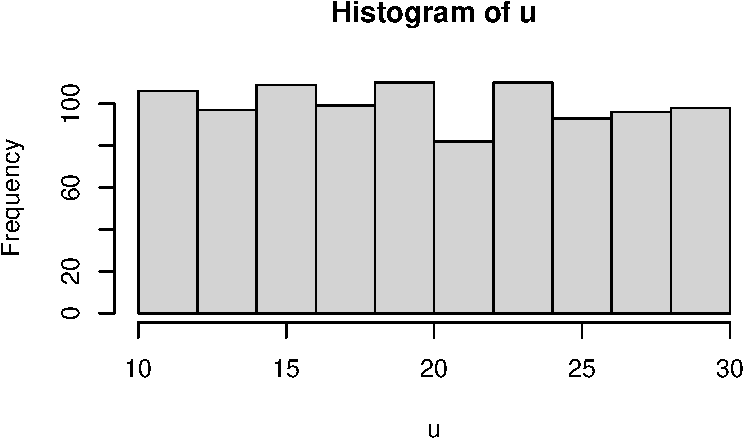
\includegraphics{051_distributions_unif_normal_files/figure-pdf/unnamed-chunk-1-1.pdf}

The histogram shows that each value (interval of values) is similarly
frequent.

\subsection{Density}\label{density-1}

Instead of a histogram, or on top of it, we often plot densities, which
is a smoother representation than the bars. The computation uses a local
density (kernel density i.e.~using a bandwidth instead of the strict
silos of the histogram). Beyond the visual, the notion of density is
important because, once it is scaled so that the entire area under the
curve sums to 1, it is interpretable as a probability.

In R in order to compute the density for an empirical distribution, we
use the \texttt{density()} function and use its returned values for
plotting. Note that we don't have frequencies anymore along the y-axis,
but values below 1, i.e.~probabilities. This is also why plotting the
density on top of a histogram requires further fine tuning (which we
leave out for now).

\begin{Shaded}
\begin{Highlighting}[]
\FunctionTok{density}\NormalTok{(u)}
\CommentTok{\#\textgreater{} }
\CommentTok{\#\textgreater{} Call:}
\CommentTok{\#\textgreater{}  density.default(x = u)}
\CommentTok{\#\textgreater{} }
\CommentTok{\#\textgreater{} Data: u (1000 obs.); Bandwidth \textquotesingle{}bw\textquotesingle{} = 1.316}
\CommentTok{\#\textgreater{} }
\CommentTok{\#\textgreater{}        x               y            }
\CommentTok{\#\textgreater{}  Min.   : 6.06   Min.   :7.237e{-}05  }
\CommentTok{\#\textgreater{}  1st Qu.:13.03   1st Qu.:1.876e{-}02  }
\CommentTok{\#\textgreater{}  Median :20.00   Median :4.731e{-}02  }
\CommentTok{\#\textgreater{}  Mean   :20.00   Mean   :3.581e{-}02  }
\CommentTok{\#\textgreater{}  3rd Qu.:26.96   3rd Qu.:5.010e{-}02  }
\CommentTok{\#\textgreater{}  Max.   :33.93   Max.   :5.278e{-}02}
\FunctionTok{plot}\NormalTok{(}\FunctionTok{density}\NormalTok{(u))}
\end{Highlighting}
\end{Shaded}

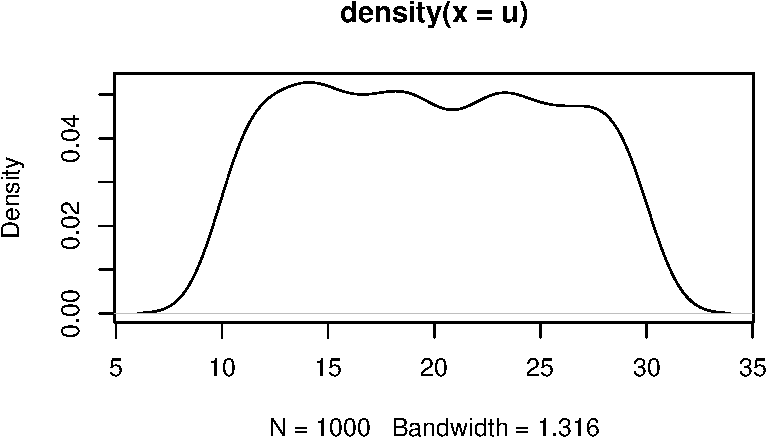
\includegraphics{051_distributions_unif_normal_files/figure-pdf/unnamed-chunk-2-1.pdf}

I order to obtaine the corresponding continuous - not numerically
simulated - density, using the same definition (i.e.~min=10 and max=30)
and a similar range for display (5 to 35), we can use \texttt{dunif()}
within the \texttt{curve()} function:

\begin{Shaded}
\begin{Highlighting}[]
\FunctionTok{curve}\NormalTok{(}\FunctionTok{dunif}\NormalTok{(x,}\AttributeTok{min=}\DecValTok{10}\NormalTok{,}\AttributeTok{max=}\DecValTok{30}\NormalTok{),}\DecValTok{5}\NormalTok{,}\DecValTok{35}\NormalTok{)}
\end{Highlighting}
\end{Shaded}

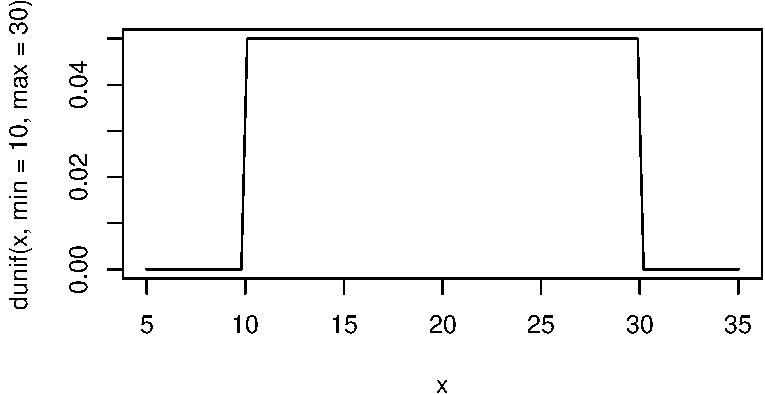
\includegraphics{051_distributions_unif_normal_files/figure-pdf/unnamed-chunk-3-1.pdf}

where we see more clearly that the probability to obtain a particular
value with a uniform distribution is constant over the defined range and
is zero otherwise.

The previous plot based on a numerical empirical generation
\texttt{runif()} is of course less regular, and there was some smoothing
at the borders of the graph due to the density being computed within a
kernel (bandwidth). Yet, the kernel is necessary in practice for having
some increment. In theory, the density can be defined over a point,
i.e.~for an infinitesimal \emph{delta} of x (\(\delta x\)), but in
practice you need a discrete interval (\(dx\)), hence the different
`look' of our two density plots: the continuous theoretical one using
\texttt{d...()} and the numerical empirical one using
\texttt{density()}.

\textbf{Mathematically, the density of a uniform distribution} is given
by (see \texttt{help(dunif)}) :

\[
\begin{align}
f_X(x) &= \dfrac{1}{b-a} &\text{ for } a \le x \le b \\
f_X(x) &= 0 &\text{ otherwise}
\end{align}
\] where \(b\) is the maximum and \(a\) the minimum whereby the
distribution is defined.

In our example we now see why the constant was at 0.05,
i.e.~(\(1/(30-10)\))

And can check it for any point x fed into \texttt{dunif()}

\begin{Shaded}
\begin{Highlighting}[]
\FunctionTok{dunif}\NormalTok{(}\FunctionTok{c}\NormalTok{(}\DecValTok{2}\NormalTok{, }\DecValTok{10}\NormalTok{, }\DecValTok{15}\NormalTok{, }\DecValTok{20}\NormalTok{, }\DecValTok{30}\NormalTok{, }\DecValTok{55}\NormalTok{),}\AttributeTok{min=}\DecValTok{10}\NormalTok{, }\AttributeTok{max=}\DecValTok{30}\NormalTok{)}
\CommentTok{\#\textgreater{} [1] 0.00 0.05 0.05 0.05 0.05 0.00}
\end{Highlighting}
\end{Shaded}

\subsection{Cumulated probabilities}\label{cumulated-probabilities}

For any continuous distribution, it is interesting to accumulate the
probabilities along the x values so that this cumulative sum indicates
the probability of randomly drawing a number that would fall below any
given value. This is called the \textbf{cumulative density function},
aka \textbf{cdf}.

Similar to the density, there is both a numerical empirical way and a
continuous theoretical way to get the cumulative density function in R,
using respectively the \texttt{ecdf()} function or the \texttt{p...()}
function corresponding to the distribution of interest.

With our empirically generated (sample) uniform distribution \(u\), we
compute the \textbf{empirical cumulative distribution function (ecdf)}
as follows:

\begin{Shaded}
\begin{Highlighting}[]
\FunctionTok{ecdf}\NormalTok{(u)}
\CommentTok{\#\textgreater{} Empirical CDF }
\CommentTok{\#\textgreater{} Call: ecdf(u)}
\CommentTok{\#\textgreater{}  x[1:1000] = 10.007, 10.015, 10.048,  ..., 29.977, 29.986}
\FunctionTok{plot}\NormalTok{(}\FunctionTok{ecdf}\NormalTok{(u))}
\end{Highlighting}
\end{Shaded}

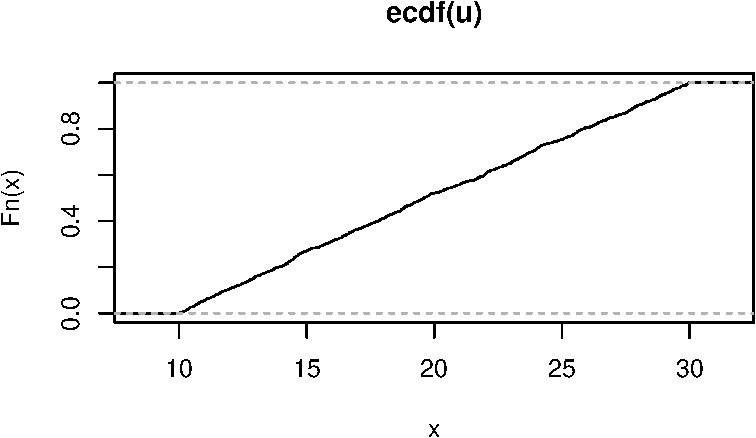
\includegraphics{051_distributions_unif_normal_files/figure-pdf/unnamed-chunk-5-1.pdf}

We can see that it is (almost) a straight line. Its slope is of course
the density we have seen above. \texttt{density()} is the derivative of
the \texttt{ecdf()} and the \texttt{ecdf()} the integral (cumulative
sum) of \texttt{density()}. For every increment of x, we increase the
probability of drawing a number below x by 0.05, up until the max (30)
is reached.

Instead of simulating numbers or using an empirical sample, we can use
the theoretical \texttt{punif()} function in this case to obtain the
theoretical cumulative density function corresponding to our parameters.

\begin{Shaded}
\begin{Highlighting}[]
\FunctionTok{curve}\NormalTok{(}\FunctionTok{punif}\NormalTok{(x,}\AttributeTok{min=}\DecValTok{10}\NormalTok{, }\AttributeTok{max=}\DecValTok{30}\NormalTok{),}\DecValTok{5}\NormalTok{,}\DecValTok{35}\NormalTok{)}
\end{Highlighting}
\end{Shaded}

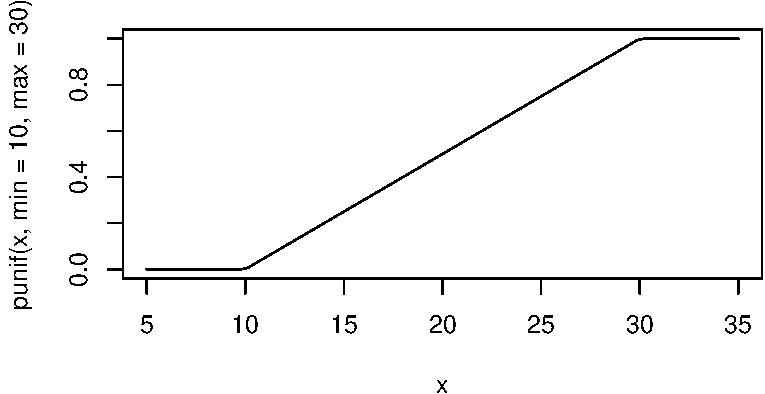
\includegraphics{051_distributions_unif_normal_files/figure-pdf/unnamed-chunk-6-1.pdf}

We see it is the theoretical continuous version of \texttt{ecdf()}
applied to our vector \(u\).

Mathematically, the cumulative distribution function of the uniform is
defined by: \[\begin{align}
F_X(x) &= 0 &\text{ for }& x < a \\
F_X(x) &= \dfrac{x-a}{b-a} &\text{ for }& a \le x \le b \\
F_X(x) &= 1 &\text{ for }& x > b
\end{align}
\]

Instead of using the \texttt{p...()} function (similar for
\texttt{d...()}) with a general x variable, we can supply a quantile (or
a set of quantiles), in order to obtain the probability of drawing a
number below this quantile.

With the uniform distribution and \texttt{punif()} it is very
straightforward because the cumulative probability simply is the
quantile as shown below

\begin{Shaded}
\begin{Highlighting}[]
\FunctionTok{punif}\NormalTok{(}\AttributeTok{q=}\FunctionTok{c}\NormalTok{(}\FloatTok{0.01}\NormalTok{,}\FloatTok{0.25}\NormalTok{,}\FloatTok{0.5}\NormalTok{,}\FloatTok{0.75}\NormalTok{,}\FloatTok{0.99}\NormalTok{))}
\CommentTok{\#\textgreater{} [1] 0.01 0.25 0.50 0.75 0.99}
\FunctionTok{punif}\NormalTok{(}\AttributeTok{min=}\DecValTok{50}\NormalTok{, }\AttributeTok{max=}\DecValTok{200}\NormalTok{, }\AttributeTok{q=}\FunctionTok{c}\NormalTok{(}\DecValTok{100}\NormalTok{)) }\CommentTok{\#the probability of drawing a number below 100 knowing the min and max are 50 and 200 and the distribution uniform is 1/3 (the range being 150 and 100 being 50 beyond the max)}
\CommentTok{\#\textgreater{} [1] 0.3333333}
\end{Highlighting}
\end{Shaded}

The last of the 4 R functions for distributions is the reverse of
\texttt{p...()}, i.e.~\texttt{q...()}, which provides the corresponding
quantile for any given probability \(p\). It is again quite
straightforward for a uniform distribution defined over the range 0 to 1
since the quantile is then the probability, and proportionally within
the defined range for other uniform distributions.

\begin{Shaded}
\begin{Highlighting}[]
\FunctionTok{curve}\NormalTok{(}\FunctionTok{qunif}\NormalTok{(x,}\AttributeTok{min=}\DecValTok{1000}\NormalTok{,}\AttributeTok{max=}\DecValTok{10000}\NormalTok{))}
\end{Highlighting}
\end{Shaded}

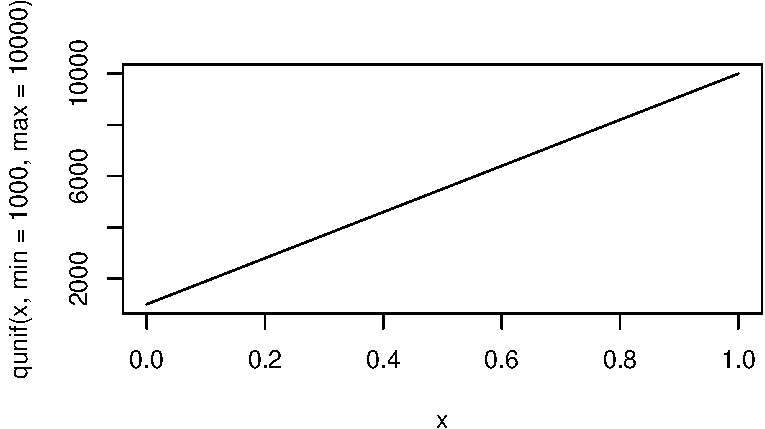
\includegraphics{051_distributions_unif_normal_files/figure-pdf/unnamed-chunk-8-1.pdf}

\begin{Shaded}
\begin{Highlighting}[]
\FunctionTok{qunif}\NormalTok{(}\AttributeTok{p=}\FloatTok{0.77}\NormalTok{,}\AttributeTok{min=}\DecValTok{1000}\NormalTok{,}\AttributeTok{max=}\DecValTok{10000}\NormalTok{)}
\CommentTok{\#\textgreater{} [1] 7930}
\end{Highlighting}
\end{Shaded}

\section{The Normal distribution}\label{the-normal-distribution}

The Normal or Gaussian distribution is the workhorse of statistics and
the most used distribution. We have seen its general bell shape earlier.

\subsection{Definition and key
characteristics:}\label{definition-and-key-characteristics-1}

A normal distribution is entirely defined by its mean and standard
deviation, which we thus need to provide for generating examples.

A normal distribution is thus denoted by
\[X \sim N(\mu, \sigma^2) \ \  \  \forall X \in R\]

where \(\mu\) and \(\sigma^2\) are the real and \textbf{unknown} mean
and variance of the studied population. It is defined over the entire
set of real numbers R.

Let's generate a normal distribution and observe its histogram.

\begin{Shaded}
\begin{Highlighting}[]
\FunctionTok{set.seed}\NormalTok{(}\DecValTok{101}\NormalTok{)}
\NormalTok{N}\OtherTok{\textless{}{-}}\FunctionTok{rnorm}\NormalTok{(}\DecValTok{100000}\NormalTok{,}\AttributeTok{mean=}\DecValTok{5}\NormalTok{,}\AttributeTok{sd=}\DecValTok{1}\NormalTok{)}
\FunctionTok{hist}\NormalTok{(N, }\AttributeTok{breaks =} \DecValTok{100}\NormalTok{)}
\end{Highlighting}
\end{Shaded}

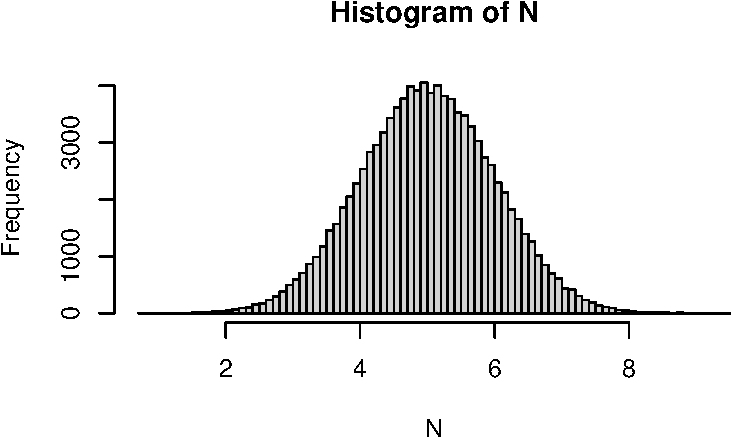
\includegraphics{051_distributions_unif_normal_files/figure-pdf/unnamed-chunk-9-1.pdf}

\begin{Shaded}
\begin{Highlighting}[]
\FunctionTok{mean}\NormalTok{(N)}
\CommentTok{\#\textgreater{} [1] 5.002881}
\FunctionTok{median}\NormalTok{(N)}
\CommentTok{\#\textgreater{} [1] 5.00018}
\FunctionTok{sd}\NormalTok{(N)}
\CommentTok{\#\textgreater{} [1] 0.9947701}
\end{Highlighting}
\end{Shaded}

\subsubsection{Symmetry}\label{symmetry}

With a numeric example the characteristics are not exact, but the mean
and standard deviations are close to those requested. We also see it is
a \textbf{symmetric distribution} and \textbf{the mean thus equals the
median} (approximately here). In other words half of the values are
below the mean and the other half above.

Symmetry also means that the skewness (3rd moment) is close to zero.
Note that its 4th moment (Kurtosis) is theoretically 3, but R takes out
this value in its computation so the kurtosis of the normal distribution
is 0, which is used as a reference. Again it is approximately given this
is only a numerical example of it.

\begin{Shaded}
\begin{Highlighting}[]
\FunctionTok{mean}\NormalTok{(N)}
\CommentTok{\#\textgreater{} [1] 5.002881}
\FunctionTok{median}\NormalTok{(N)}
\CommentTok{\#\textgreater{} [1] 5.00018}
\NormalTok{e1071}\SpecialCharTok{::}\FunctionTok{skewness}\NormalTok{(N)}
\CommentTok{\#\textgreater{} [1] {-}0.001284229}
\NormalTok{e1071}\SpecialCharTok{::}\FunctionTok{kurtosis}\NormalTok{(N)}
\CommentTok{\#\textgreater{} [1] 0.004644777}
\end{Highlighting}
\end{Shaded}

We can look at the impact of generating a smaller sample, to show how
means, medians, skewness or kurtosis and the histogram vary quite a bit
from the expected when the size of the sample decreases:

\begin{Shaded}
\begin{Highlighting}[]
\NormalTok{N10000}\OtherTok{\textless{}{-}}\FunctionTok{rnorm}\NormalTok{(}\DecValTok{10000}\NormalTok{,}\AttributeTok{mean=}\DecValTok{5}\NormalTok{,}\AttributeTok{sd=}\DecValTok{1}\NormalTok{)}
\NormalTok{N1000}\OtherTok{\textless{}{-}}\FunctionTok{rnorm}\NormalTok{(}\DecValTok{1000}\NormalTok{,}\AttributeTok{mean=}\DecValTok{5}\NormalTok{,}\AttributeTok{sd=}\DecValTok{1}\NormalTok{)}
\NormalTok{N100}\OtherTok{\textless{}{-}}\FunctionTok{rnorm}\NormalTok{(}\DecValTok{100}\NormalTok{,}\AttributeTok{mean=}\DecValTok{5}\NormalTok{,}\AttributeTok{sd=}\DecValTok{1}\NormalTok{)}
\NormalTok{N10}\OtherTok{\textless{}{-}}\FunctionTok{rnorm}\NormalTok{(}\DecValTok{10}\NormalTok{,}\AttributeTok{mean=}\DecValTok{5}\NormalTok{,}\AttributeTok{sd=}\DecValTok{1}\NormalTok{)}
\FunctionTok{hist}\NormalTok{(N10000, }\AttributeTok{breaks =} \DecValTok{100}\NormalTok{, }\AttributeTok{border=}\ConstantTok{NA}\NormalTok{, }\AttributeTok{col=}\FunctionTok{rgb}\NormalTok{(}\DecValTok{1}\NormalTok{, }\FloatTok{0.5}\NormalTok{, }\DecValTok{1}\NormalTok{, }\FloatTok{0.5}\NormalTok{))}
\end{Highlighting}
\end{Shaded}

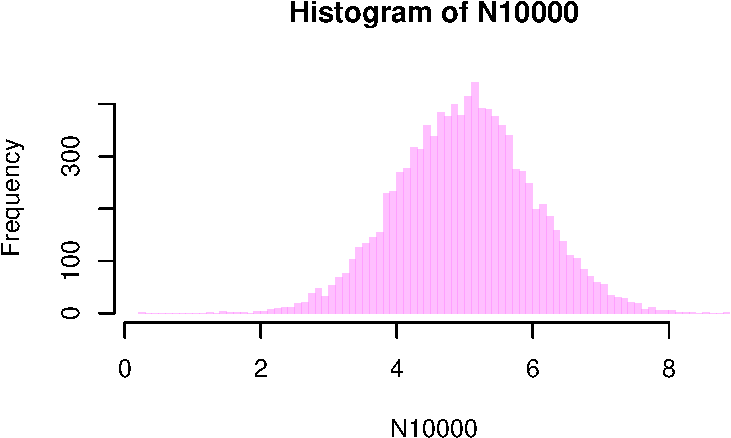
\includegraphics{051_distributions_unif_normal_files/figure-pdf/unnamed-chunk-11-1.pdf}

\begin{Shaded}
\begin{Highlighting}[]
\FunctionTok{hist}\NormalTok{(N1000, }\AttributeTok{breaks =} \DecValTok{100}\NormalTok{, }\AttributeTok{border=}\ConstantTok{NA}\NormalTok{, }\AttributeTok{col=}\FunctionTok{rgb}\NormalTok{(}\DecValTok{1}\NormalTok{, }\FloatTok{0.5}\NormalTok{, }\DecValTok{1}\NormalTok{, }\FloatTok{0.5}\NormalTok{))}
\end{Highlighting}
\end{Shaded}

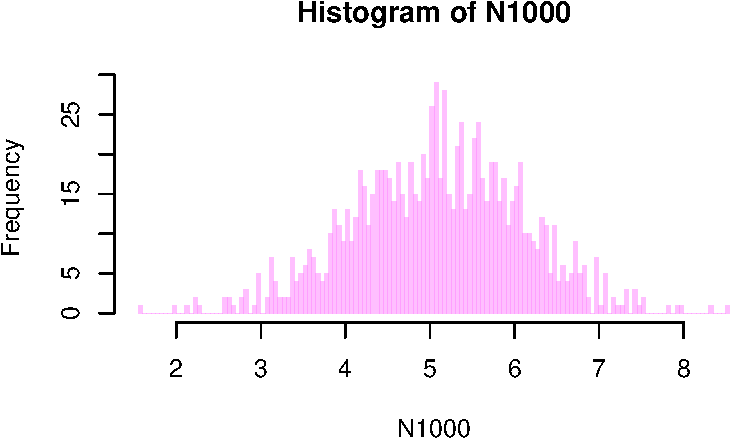
\includegraphics{051_distributions_unif_normal_files/figure-pdf/unnamed-chunk-11-2.pdf}

\begin{Shaded}
\begin{Highlighting}[]
\FunctionTok{hist}\NormalTok{(N100, }\AttributeTok{breaks =} \DecValTok{100}\NormalTok{, }\AttributeTok{border=}\ConstantTok{NA}\NormalTok{, }\AttributeTok{col=}\FunctionTok{rgb}\NormalTok{(}\DecValTok{1}\NormalTok{, }\FloatTok{0.5}\NormalTok{, }\DecValTok{1}\NormalTok{, }\FloatTok{0.5}\NormalTok{))}
\end{Highlighting}
\end{Shaded}

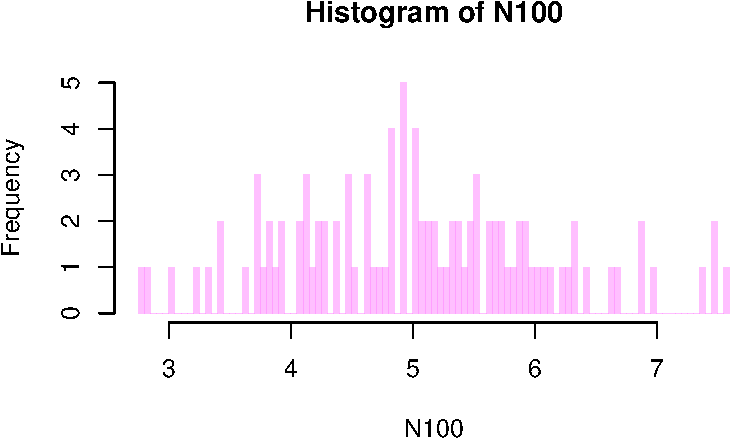
\includegraphics{051_distributions_unif_normal_files/figure-pdf/unnamed-chunk-11-3.pdf}

\begin{Shaded}
\begin{Highlighting}[]
\FunctionTok{hist}\NormalTok{(N10, }\AttributeTok{breaks =} \DecValTok{100}\NormalTok{, }\AttributeTok{border=}\ConstantTok{NA}\NormalTok{, }\AttributeTok{col=}\FunctionTok{rgb}\NormalTok{(}\DecValTok{1}\NormalTok{, }\FloatTok{0.5}\NormalTok{, }\DecValTok{1}\NormalTok{, }\FloatTok{0.5}\NormalTok{))}
\end{Highlighting}
\end{Shaded}

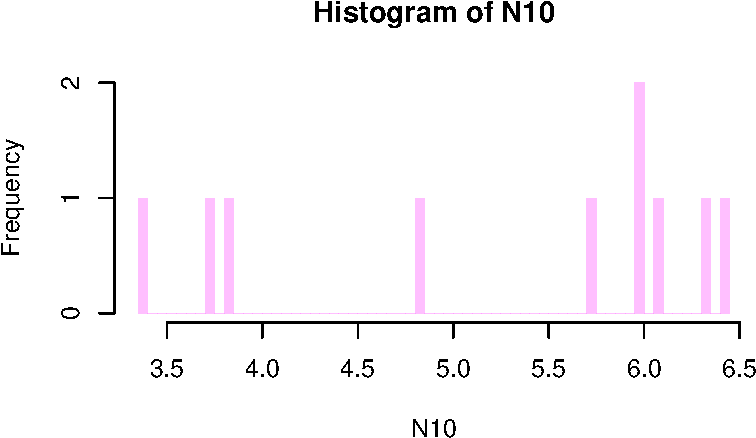
\includegraphics{051_distributions_unif_normal_files/figure-pdf/unnamed-chunk-11-4.pdf}

\subsubsection{Quantiles and standard
deviations}\label{quantiles-and-standard-deviations}

A key feature of the normal distribution is that approximately
\textbf{68\% of its values fall within one standard deviation from the
mean} (both side as it is symmetrical), 95\% within two standard
deviations, and 99.7\% within three standard deviations. This
characteristic is heavily used to make probability tests.

\subsection{Density}\label{density-2}

We know compute the empirical density for our sample, showing the
previous histogram with large sample size was indeed bell-shaped (but
not so much the small sample examples)

\begin{Shaded}
\begin{Highlighting}[]
\FunctionTok{density}\NormalTok{(N)}
\CommentTok{\#\textgreater{} }
\CommentTok{\#\textgreater{} Call:}
\CommentTok{\#\textgreater{}  density.default(x = N)}
\CommentTok{\#\textgreater{} }
\CommentTok{\#\textgreater{} Data: N (100000 obs.);   Bandwidth \textquotesingle{}bw\textquotesingle{} = 0.08953}
\CommentTok{\#\textgreater{} }
\CommentTok{\#\textgreater{}        x                y            }
\CommentTok{\#\textgreater{}  Min.   :0.5144   Min.   :6.700e{-}07  }
\CommentTok{\#\textgreater{}  1st Qu.:2.8273   1st Qu.:1.105e{-}03  }
\CommentTok{\#\textgreater{}  Median :5.1403   Median :2.590e{-}02  }
\CommentTok{\#\textgreater{}  Mean   :5.1403   Mean   :1.079e{-}01  }
\CommentTok{\#\textgreater{}  3rd Qu.:7.4533   3rd Qu.:2.049e{-}01  }
\CommentTok{\#\textgreater{}  Max.   :9.7663   Max.   :3.981e{-}01}
\FunctionTok{plot}\NormalTok{(}\FunctionTok{density}\NormalTok{(N)) }\CommentTok{\#The integral of the density being 1, overlaying on top of the histogram doesn\textquotesingle{}t work because it depends on the heights of the bar which itself depends on the number of bars. See Crawley, p215 for such a manipulation or later with ggplot}
\end{Highlighting}
\end{Shaded}

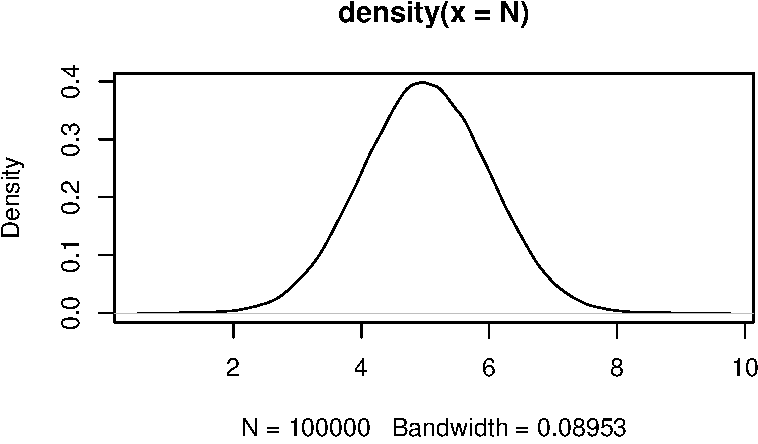
\includegraphics{051_distributions_unif_normal_files/figure-pdf/unnamed-chunk-12-1.pdf}

\begin{Shaded}
\begin{Highlighting}[]
\FunctionTok{plot}\NormalTok{(}\FunctionTok{density}\NormalTok{(N10000), }\AttributeTok{main=}\StringTok{"Varying sample size"}\NormalTok{, }\AttributeTok{col=}\FunctionTok{rgb}\NormalTok{(}\DecValTok{1}\NormalTok{, }\FloatTok{0.5}\NormalTok{, }\DecValTok{1}\NormalTok{, }\FloatTok{0.5}\NormalTok{), }\AttributeTok{lwd=}\DecValTok{5}\NormalTok{,}\AttributeTok{xlab=}\StringTok{"x"}\NormalTok{)}
\FunctionTok{lines}\NormalTok{(}\FunctionTok{density}\NormalTok{(N1000), }\AttributeTok{col=}\FunctionTok{rgb}\NormalTok{(}\DecValTok{1}\NormalTok{, }\FloatTok{0.5}\NormalTok{, }\DecValTok{1}\NormalTok{, }\FloatTok{0.5}\NormalTok{),}\AttributeTok{lwd=}\DecValTok{3}\NormalTok{)}
\FunctionTok{lines}\NormalTok{(}\FunctionTok{density}\NormalTok{(N100), }\AttributeTok{col=}\FunctionTok{rgb}\NormalTok{(}\DecValTok{1}\NormalTok{, }\FloatTok{0.5}\NormalTok{, }\DecValTok{1}\NormalTok{, }\FloatTok{0.5}\NormalTok{), }\AttributeTok{lwd=}\DecValTok{2}\NormalTok{)}
\FunctionTok{lines}\NormalTok{(}\FunctionTok{density}\NormalTok{(N10), }\AttributeTok{col=}\FunctionTok{rgb}\NormalTok{(}\DecValTok{1}\NormalTok{, }\FloatTok{0.5}\NormalTok{, }\DecValTok{1}\NormalTok{, }\FloatTok{0.5}\NormalTok{), }\AttributeTok{lwd=}\DecValTok{1}\NormalTok{)}
\end{Highlighting}
\end{Shaded}

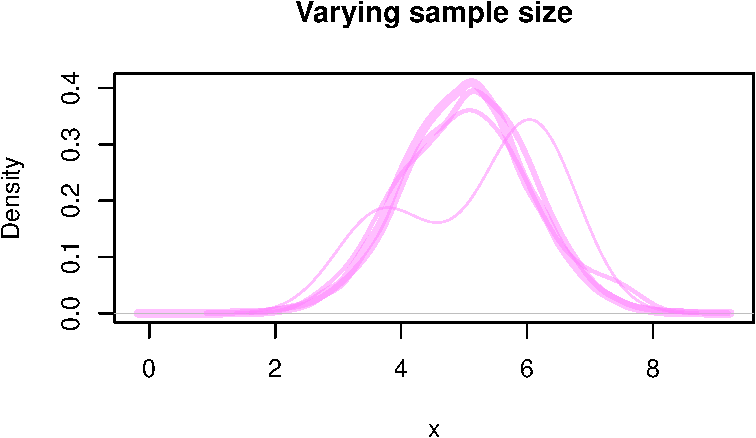
\includegraphics{051_distributions_unif_normal_files/figure-pdf/unnamed-chunk-13-1.pdf}

To obtain the corresponding theoretical function of the density, using
the same mean and standard deviation, and along the same range of x
values (0 to 10) for the graph, we can use \texttt{dnorm()} instead of
the empirical function \texttt{density()}. Observe also that the density
of a normal distribution at its peak, i.e.~at the mean or median, is
around 0.39.

\begin{Shaded}
\begin{Highlighting}[]
\FunctionTok{curve}\NormalTok{(}\FunctionTok{dnorm}\NormalTok{(x,}\AttributeTok{mean=}\DecValTok{5}\NormalTok{,}\AttributeTok{sd=}\DecValTok{1}\NormalTok{),}\DecValTok{0}\NormalTok{,}\DecValTok{10}\NormalTok{)}
\end{Highlighting}
\end{Shaded}

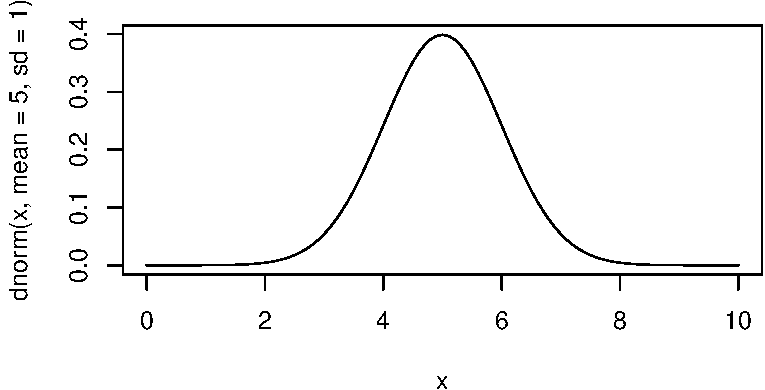
\includegraphics{051_distributions_unif_normal_files/figure-pdf/unnamed-chunk-14-1.pdf}

\begin{Shaded}
\begin{Highlighting}[]
\FunctionTok{dnorm}\NormalTok{(}\DecValTok{5}\NormalTok{, }\AttributeTok{mean=}\DecValTok{5}\NormalTok{,}\AttributeTok{sd=}\DecValTok{1}\NormalTok{)}
\CommentTok{\#\textgreater{} [1] 0.3989423}
\end{Highlighting}
\end{Shaded}

Mathematically, the density of a norma distribution is given by the
following, which is used within \texttt{dnorm()} (see
\texttt{help(dnorm)}) :

\[f(x) = \dfrac {1}{\sqrt{2 \sigma^2 \pi}} \exp{(- \dfrac{1}{2} \dfrac{(x-\mu)^2}{\sigma^2})}\]

In the following, we play with the two defining parameters, mean and
standard deviation, to show how each impact the shape of the
distribution while keeping the second parameter constant:

\begin{Shaded}
\begin{Highlighting}[]
\FunctionTok{curve}\NormalTok{(}\FunctionTok{dnorm}\NormalTok{(x,}\AttributeTok{mean=}\DecValTok{0}\NormalTok{,}\AttributeTok{sd=}\DecValTok{1}\NormalTok{),}\SpecialCharTok{{-}}\DecValTok{5}\NormalTok{,}\DecValTok{5}\NormalTok{, }\AttributeTok{lty=}\DecValTok{1}\NormalTok{)}
\FunctionTok{curve}\NormalTok{(}\FunctionTok{dnorm}\NormalTok{(x,}\AttributeTok{mean=}\SpecialCharTok{{-}}\DecValTok{2}\NormalTok{,}\AttributeTok{sd=}\DecValTok{1}\NormalTok{),}\SpecialCharTok{{-}}\DecValTok{5}\NormalTok{,}\DecValTok{5}\NormalTok{, }\AttributeTok{lty=}\DecValTok{2}\NormalTok{, }\AttributeTok{add=}\ConstantTok{TRUE}\NormalTok{)}
\FunctionTok{curve}\NormalTok{(}\FunctionTok{dnorm}\NormalTok{(x,}\AttributeTok{mean=}\DecValTok{1}\NormalTok{,}\AttributeTok{sd=}\DecValTok{1}\NormalTok{),}\SpecialCharTok{{-}}\DecValTok{5}\NormalTok{,}\DecValTok{5}\NormalTok{, }\AttributeTok{lty=}\DecValTok{3}\NormalTok{, }\AttributeTok{add=}\ConstantTok{TRUE}\NormalTok{)}
\end{Highlighting}
\end{Shaded}

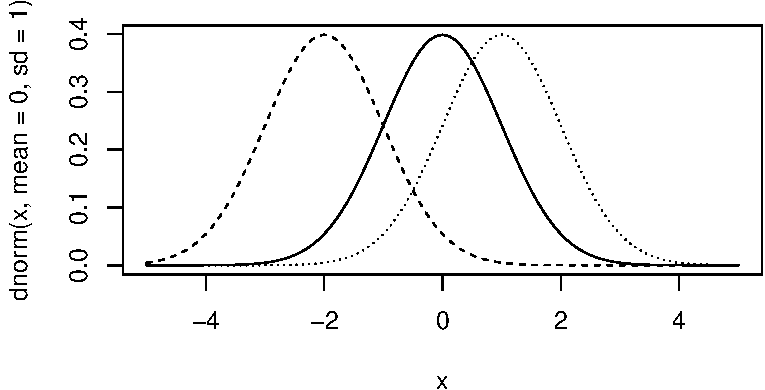
\includegraphics{051_distributions_unif_normal_files/figure-pdf/unnamed-chunk-15-1.pdf}

\begin{Shaded}
\begin{Highlighting}[]

\FunctionTok{curve}\NormalTok{(}\FunctionTok{dnorm}\NormalTok{(x,}\AttributeTok{mean=}\DecValTok{0}\NormalTok{,}\AttributeTok{sd=}\DecValTok{1}\NormalTok{),}\SpecialCharTok{{-}}\DecValTok{5}\NormalTok{,}\DecValTok{5}\NormalTok{, }\AttributeTok{lty=}\DecValTok{1}\NormalTok{, }\AttributeTok{col=}\StringTok{"blue"}\NormalTok{)}
\FunctionTok{curve}\NormalTok{(}\FunctionTok{dnorm}\NormalTok{(x,}\AttributeTok{mean=}\DecValTok{0}\NormalTok{,}\AttributeTok{sd=}\FloatTok{0.7}\NormalTok{),}\SpecialCharTok{{-}}\DecValTok{5}\NormalTok{,}\DecValTok{5}\NormalTok{, }\AttributeTok{lty=}\DecValTok{2}\NormalTok{, }\AttributeTok{col=}\StringTok{"blue"}\NormalTok{, }\AttributeTok{add=}\ConstantTok{TRUE}\NormalTok{)}
\FunctionTok{curve}\NormalTok{(}\FunctionTok{dnorm}\NormalTok{(x,}\AttributeTok{mean=}\DecValTok{0}\NormalTok{,}\AttributeTok{sd=}\DecValTok{2}\NormalTok{),}\SpecialCharTok{{-}}\DecValTok{5}\NormalTok{,}\DecValTok{5}\NormalTok{, }\AttributeTok{lty=}\DecValTok{3}\NormalTok{, }\AttributeTok{col=}\StringTok{"blue"}\NormalTok{, }\AttributeTok{add=}\ConstantTok{TRUE}\NormalTok{)}
\end{Highlighting}
\end{Shaded}

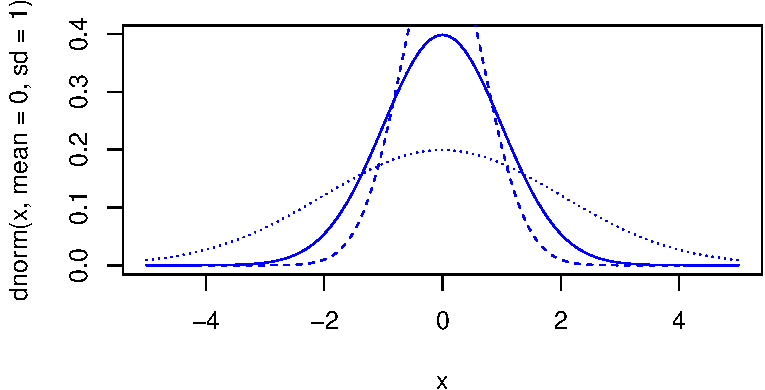
\includegraphics{051_distributions_unif_normal_files/figure-pdf/unnamed-chunk-15-2.pdf}

The general shape is not influenced by the mean as the distribution is
simply translated along x. When the standard deviation increases, as
expected, the distribution is flatter but still around the same mean.

If we generate two new (large) samples with a different standard
deviation, we see the flattening. However, the shape is still a bell
shape and the \textbf{kurtosis will not pick the difference!}. The
peakness referred to by the kurtosis is one that is relative to the
corresponding normal distribution (thus knowing its variance).

\begin{Shaded}
\begin{Highlighting}[]
\FunctionTok{set.seed}\NormalTok{(}\DecValTok{101}\NormalTok{)}
\NormalTok{Z}\OtherTok{\textless{}{-}}\FunctionTok{rnorm}\NormalTok{(}\DecValTok{1000000}\NormalTok{,}\AttributeTok{mean=}\DecValTok{0}\NormalTok{,}\AttributeTok{sd=}\DecValTok{1}\NormalTok{)}
\NormalTok{Flat}\OtherTok{\textless{}{-}}\FunctionTok{rnorm}\NormalTok{(}\DecValTok{1000000}\NormalTok{,}\AttributeTok{mean=}\DecValTok{0}\NormalTok{,}\AttributeTok{sd=}\DecValTok{3}\NormalTok{)}
\FunctionTok{plot}\NormalTok{(}\FunctionTok{density}\NormalTok{(Z))}
\FunctionTok{lines}\NormalTok{(}\FunctionTok{density}\NormalTok{(Flat))}
\end{Highlighting}
\end{Shaded}

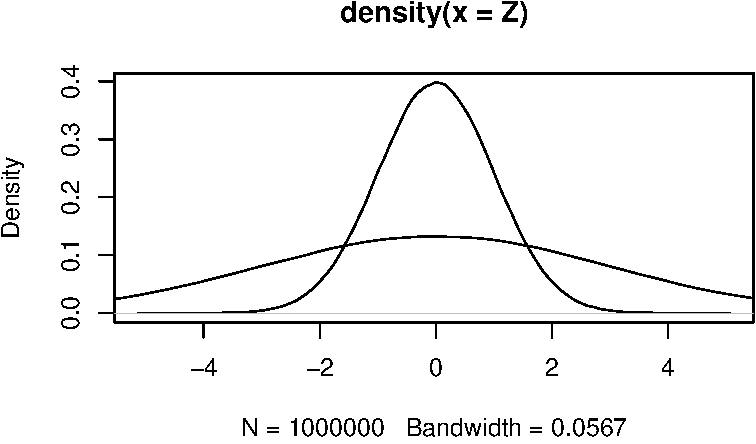
\includegraphics{051_distributions_unif_normal_files/figure-pdf/unnamed-chunk-16-1.pdf}

\begin{Shaded}
\begin{Highlighting}[]
\NormalTok{e1071}\SpecialCharTok{::}\FunctionTok{kurtosis}\NormalTok{(Z)}
\CommentTok{\#\textgreater{} [1] {-}0.005819773}
\NormalTok{e1071}\SpecialCharTok{::}\FunctionTok{kurtosis}\NormalTok{(Flat)}
\CommentTok{\#\textgreater{} [1] {-}0.002299496}
\end{Highlighting}
\end{Shaded}

We know explore graphically and with the function \texttt{dnorm()} the
other property of the normal distribution by which we know that in a
normal distribution, the range of values situated - + - 1 standard
deviation from the mean represents 68\% of the data - + - 2 standard
deviations from the mean represents 95\% of the data - + - 3 standard
deviations from the mean represents 99.7\% of the data

\begin{Shaded}
\begin{Highlighting}[]
\FunctionTok{curve}\NormalTok{(}\FunctionTok{dnorm}\NormalTok{(x, }\DecValTok{0}\NormalTok{, }\DecValTok{1}\NormalTok{), }\AttributeTok{col =} \StringTok{\textquotesingle{}green\textquotesingle{}}\NormalTok{, }\AttributeTok{lwd =} \DecValTok{8}\NormalTok{, }\AttributeTok{xlim =} \FunctionTok{c}\NormalTok{(}\SpecialCharTok{{-}}\DecValTok{3}\NormalTok{, }\DecValTok{3}\NormalTok{), }\AttributeTok{main =} \StringTok{\textquotesingle{}Density function of X \textasciitilde{} N(0,1)}\SpecialCharTok{\textbackslash{}n}\StringTok{ Intervals\textquotesingle{}}\NormalTok{, }\AttributeTok{ylab =} \StringTok{\textquotesingle{}f(x)\textquotesingle{}}\NormalTok{)}
\FunctionTok{curve}\NormalTok{(}\FunctionTok{dnorm}\NormalTok{(x, }\DecValTok{0}\NormalTok{, }\DecValTok{1}\NormalTok{), }\AttributeTok{add =} \ConstantTok{TRUE}\NormalTok{, }\AttributeTok{col =} \StringTok{\textquotesingle{}gold\textquotesingle{}}\NormalTok{, }\AttributeTok{lwd =} \DecValTok{5}\NormalTok{, }\AttributeTok{xlim =} \FunctionTok{c}\NormalTok{(}\SpecialCharTok{{-}}\DecValTok{2}\NormalTok{, }\DecValTok{2}\NormalTok{))}
\FunctionTok{curve}\NormalTok{(}\FunctionTok{dnorm}\NormalTok{(x, }\DecValTok{0}\NormalTok{, }\DecValTok{1}\NormalTok{), }\AttributeTok{add =} \ConstantTok{TRUE}\NormalTok{, }\AttributeTok{col =} \StringTok{"red"}\NormalTok{, }\AttributeTok{lwd =} \DecValTok{2}\NormalTok{, }\AttributeTok{xlim =} \FunctionTok{c}\NormalTok{(}\SpecialCharTok{{-}}\DecValTok{1}\NormalTok{, }\DecValTok{1}\NormalTok{))}
\FunctionTok{abline}\NormalTok{(}\AttributeTok{v =} \DecValTok{0}\NormalTok{, }\AttributeTok{col =} \StringTok{"grey"}\NormalTok{, }\AttributeTok{lty =} \DecValTok{1}\NormalTok{)}
\FunctionTok{abline}\NormalTok{(}\AttributeTok{v =} \FunctionTok{c}\NormalTok{(}\SpecialCharTok{{-}}\DecValTok{1}\NormalTok{, }\DecValTok{1}\NormalTok{), }\AttributeTok{col =} \StringTok{"red"}\NormalTok{, }\AttributeTok{lty =} \DecValTok{3}\NormalTok{)}
\FunctionTok{abline}\NormalTok{(}\AttributeTok{v =} \FunctionTok{c}\NormalTok{(}\SpecialCharTok{{-}}\DecValTok{2}\NormalTok{, }\DecValTok{2}\NormalTok{), }\AttributeTok{col =} \StringTok{"gold"}\NormalTok{, }\AttributeTok{lty =} \DecValTok{3}\NormalTok{)}
\FunctionTok{abline}\NormalTok{(}\AttributeTok{v =} \FunctionTok{c}\NormalTok{(}\SpecialCharTok{{-}}\DecValTok{3}\NormalTok{, }\DecValTok{3}\NormalTok{), }\AttributeTok{col =} \StringTok{"green"}\NormalTok{, }\AttributeTok{lty =} \DecValTok{3}\NormalTok{)}
\FunctionTok{legend}\NormalTok{(}\StringTok{"topleft"}\NormalTok{, }\AttributeTok{lwd =} \FunctionTok{c}\NormalTok{(}\DecValTok{2}\NormalTok{,}\DecValTok{5}\NormalTok{,}\DecValTok{8}\NormalTok{),}
       \AttributeTok{legend =} \FunctionTok{c}\NormalTok{(}\StringTok{"68\% in [ mu +/{-} sigma ]"}\NormalTok{, }
                  \StringTok{"95\% in [ mu +/{-} 2*sigma ]"}\NormalTok{, }
                  \StringTok{"99.7\% in [ mu +/{-} 3*sigma ]"}\NormalTok{),}
       \AttributeTok{col =} \FunctionTok{c}\NormalTok{(}\StringTok{"red"}\NormalTok{, }\StringTok{\textquotesingle{}gold\textquotesingle{}}\NormalTok{, }\StringTok{\textquotesingle{}green\textquotesingle{}}\NormalTok{))}
\end{Highlighting}
\end{Shaded}

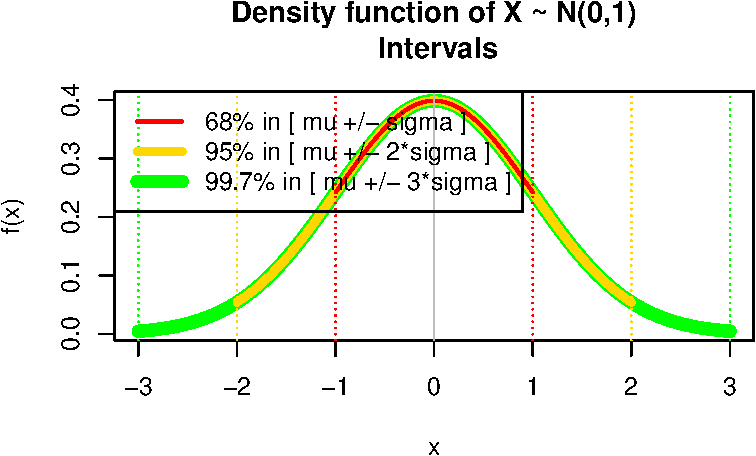
\includegraphics{051_distributions_unif_normal_files/figure-pdf/unnamed-chunk-17-1.pdf}

\begin{Shaded}
\begin{Highlighting}[]

\FunctionTok{curve}\NormalTok{(}\FunctionTok{dnorm}\NormalTok{(x, }\DecValTok{0}\NormalTok{, }\DecValTok{1}\NormalTok{), }\AttributeTok{col =} \StringTok{\textquotesingle{}green\textquotesingle{}}\NormalTok{, }\AttributeTok{lwd =} \DecValTok{8}\NormalTok{, }\AttributeTok{xlim =} \FunctionTok{c}\NormalTok{(}\SpecialCharTok{{-}}\FloatTok{2.58}\NormalTok{, }\FloatTok{2.58}\NormalTok{), }\AttributeTok{main =} \StringTok{\textquotesingle{}Density function of X \textasciitilde{} N(0,1)}\SpecialCharTok{\textbackslash{}n}\StringTok{ Intervals\textquotesingle{}}\NormalTok{, }\AttributeTok{ylab =} \StringTok{\textquotesingle{}f(x)\textquotesingle{}}\NormalTok{)}
\FunctionTok{curve}\NormalTok{(}\FunctionTok{dnorm}\NormalTok{(x, }\DecValTok{0}\NormalTok{, }\DecValTok{1}\NormalTok{), }\AttributeTok{add =} \ConstantTok{TRUE}\NormalTok{, }\AttributeTok{col =} \StringTok{\textquotesingle{}gold\textquotesingle{}}\NormalTok{, }\AttributeTok{lwd =} \DecValTok{5}\NormalTok{, }\AttributeTok{xlim =} \FunctionTok{c}\NormalTok{(}\SpecialCharTok{{-}}\FloatTok{1.96}\NormalTok{, }\FloatTok{1.96}\NormalTok{))}
\FunctionTok{curve}\NormalTok{(}\FunctionTok{dnorm}\NormalTok{(x, }\DecValTok{0}\NormalTok{, }\DecValTok{1}\NormalTok{), }\AttributeTok{add =} \ConstantTok{TRUE}\NormalTok{, }\AttributeTok{col =} \StringTok{"red"}\NormalTok{, }\AttributeTok{lwd =} \DecValTok{2}\NormalTok{, }\AttributeTok{xlim =} \FunctionTok{c}\NormalTok{(}\SpecialCharTok{{-}}\FloatTok{1.645}\NormalTok{, }\FloatTok{1.645}\NormalTok{))}
\FunctionTok{abline}\NormalTok{(}\AttributeTok{v =} \DecValTok{0}\NormalTok{, }\AttributeTok{col =} \StringTok{"grey"}\NormalTok{, }\AttributeTok{lty =} \DecValTok{1}\NormalTok{)}
\FunctionTok{abline}\NormalTok{(}\AttributeTok{v =} \FunctionTok{c}\NormalTok{(}\SpecialCharTok{{-}}\FloatTok{1.645}\NormalTok{, }\FloatTok{1.645}\NormalTok{), }\AttributeTok{col =} \StringTok{"red"}\NormalTok{, }\AttributeTok{lty =} \DecValTok{3}\NormalTok{)}
\FunctionTok{abline}\NormalTok{(}\AttributeTok{v =} \FunctionTok{c}\NormalTok{(}\SpecialCharTok{{-}}\FloatTok{1.96}\NormalTok{, }\FloatTok{1.96}\NormalTok{), }\AttributeTok{col =} \StringTok{\textquotesingle{}gold\textquotesingle{}}\NormalTok{, }\AttributeTok{lty =} \DecValTok{3}\NormalTok{)}
\FunctionTok{abline}\NormalTok{(}\AttributeTok{v =} \FunctionTok{c}\NormalTok{(}\SpecialCharTok{{-}}\FloatTok{2.58}\NormalTok{, }\FloatTok{2.58}\NormalTok{), }\AttributeTok{col =} \StringTok{\textquotesingle{}green\textquotesingle{}}\NormalTok{, }\AttributeTok{lty =} \DecValTok{3}\NormalTok{)}
\FunctionTok{legend}\NormalTok{(}\StringTok{"topleft"}\NormalTok{, }\AttributeTok{lty =} \DecValTok{1}\NormalTok{, }\AttributeTok{lwd =} \FunctionTok{c}\NormalTok{(}\DecValTok{2}\NormalTok{,}\DecValTok{5}\NormalTok{,}\DecValTok{8}\NormalTok{),}
       \AttributeTok{legend =} \FunctionTok{c}\NormalTok{(}\StringTok{"90\% in [ +/{-} 1.645 ]"}\NormalTok{, }
                  \StringTok{"95\% in [ +/{-} 1.96 ]"}\NormalTok{, }
                  \StringTok{"99\% in [ +/{-} 2.58 ]"}\NormalTok{),}
       \AttributeTok{col =} \FunctionTok{c}\NormalTok{(}\StringTok{"red"}\NormalTok{, }\StringTok{\textquotesingle{}gold\textquotesingle{}}\NormalTok{, }\StringTok{\textquotesingle{}green\textquotesingle{}}\NormalTok{))}
\end{Highlighting}
\end{Shaded}

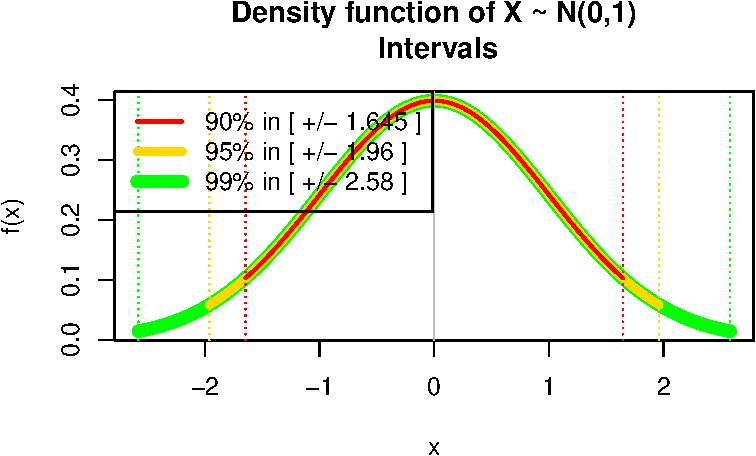
\includegraphics{051_distributions_unif_normal_files/figure-pdf/unnamed-chunk-18-1.pdf}

\subsection{Cumulated probabilities}\label{cumulated-probabilities-1}

Similar to the case of the uniform distribution, we can also look at the
cumulative probability. Theoretically we use \texttt{pnorm()}, which it
the equivalent of the uniform \texttt{punif()}. Empirically we can use
the \texttt{ecdf()} function again since it makes no assumption on the
distribution (for it is used to explore empirical material).

\begin{Shaded}
\begin{Highlighting}[]
\FunctionTok{curve}\NormalTok{(}\FunctionTok{pnorm}\NormalTok{(x),}\SpecialCharTok{{-}}\DecValTok{4}\NormalTok{,}\DecValTok{4}\NormalTok{) }\CommentTok{\#theoretical (unit normal)}
\end{Highlighting}
\end{Shaded}

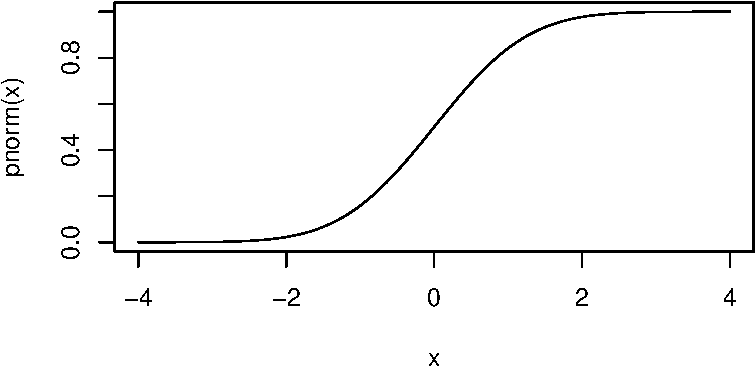
\includegraphics{051_distributions_unif_normal_files/figure-pdf/unnamed-chunk-19-1.pdf}

\begin{Shaded}
\begin{Highlighting}[]

\NormalTok{N}\OtherTok{\textless{}{-}}\FunctionTok{rnorm}\NormalTok{(}\DecValTok{100}\NormalTok{)}
\FunctionTok{plot}\NormalTok{(}\FunctionTok{ecdf}\NormalTok{(N)) }\CommentTok{\#sample}
\end{Highlighting}
\end{Shaded}

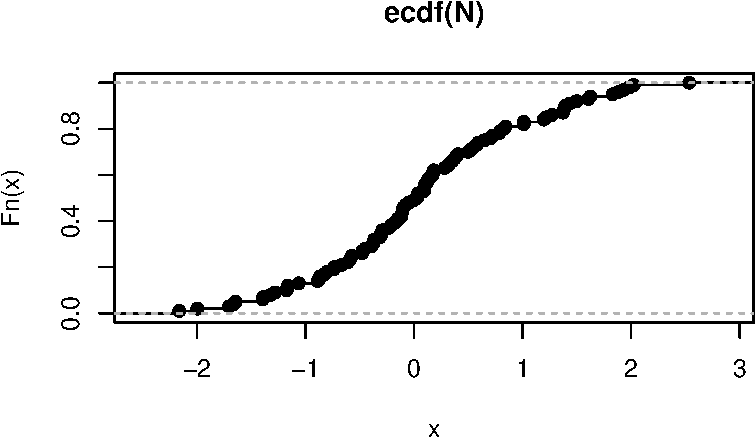
\includegraphics{051_distributions_unif_normal_files/figure-pdf/unnamed-chunk-19-2.pdf}

We see that the bell shape of the density (from \texttt{dnorm()}) is the
derivative of an S-shaped function. The probability of drawing a number
below a certain value is not constantly increasing as in the case of the
uniform distribution. Rather, the probability grows slowly for lower
values, then very quickly around the mean where the mass of data is
found, then slows downs and plateau again for higher values.

Mathematically, the cumulative distribution function of the standard
normal distribution is the integral of the probability distribution
\(f(x)\) defined earlier. It is often denoted by \(\Phi(x)\) but has no
closed solution and thus statistical software compute values
numerically.

\begin{Shaded}
\begin{Highlighting}[]
\FunctionTok{curve}\NormalTok{(}\FunctionTok{pnorm}\NormalTok{(x, }\DecValTok{0}\NormalTok{, }\DecValTok{1}\NormalTok{),}\SpecialCharTok{{-}}\DecValTok{6}\NormalTok{,}\DecValTok{6}\NormalTok{, }\AttributeTok{type=}\StringTok{\textquotesingle{}l\textquotesingle{}}\NormalTok{, }\AttributeTok{col=}\DecValTok{2}\NormalTok{, }\AttributeTok{ylab =} \StringTok{\textquotesingle{}F(x)\textquotesingle{}}\NormalTok{, }
     \AttributeTok{main =} \StringTok{\textquotesingle{}Cumulative Distribution Function of N(mu ; 1)\textquotesingle{}}\NormalTok{)}
\FunctionTok{curve}\NormalTok{(}\FunctionTok{pnorm}\NormalTok{(x, }\DecValTok{2}\NormalTok{, }\DecValTok{1}\NormalTok{), }\AttributeTok{col=}\StringTok{\textquotesingle{}darkorange\textquotesingle{}}\NormalTok{, }\AttributeTok{add=}\ConstantTok{TRUE}\NormalTok{)}
\FunctionTok{curve}\NormalTok{(}\FunctionTok{pnorm}\NormalTok{(x, }\DecValTok{4}\NormalTok{, }\DecValTok{1}\NormalTok{), }\AttributeTok{col=}\StringTok{\textquotesingle{}gold\textquotesingle{}}\NormalTok{, }\AttributeTok{add=}\ConstantTok{TRUE}\NormalTok{)}
\FunctionTok{legend}\NormalTok{(}\StringTok{"topleft"}\NormalTok{, }\AttributeTok{lty =} \DecValTok{1}\NormalTok{,}
       \AttributeTok{legend =} \FunctionTok{c}\NormalTok{(}\StringTok{"mu = 0"}\NormalTok{, }\StringTok{"mu = 2"}\NormalTok{, }\StringTok{"mu = 4"}\NormalTok{),}
       \AttributeTok{col =} \FunctionTok{c}\NormalTok{(}\DecValTok{2}\NormalTok{, }\StringTok{\textquotesingle{}darkorange\textquotesingle{}}\NormalTok{, }\StringTok{\textquotesingle{}gold\textquotesingle{}}\NormalTok{))}
\end{Highlighting}
\end{Shaded}

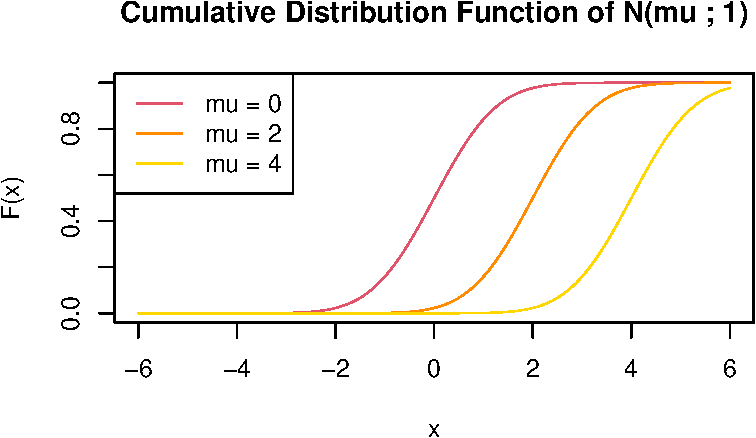
\includegraphics{051_distributions_unif_normal_files/figure-pdf/normalCum2-1.pdf}

\begin{Shaded}
\begin{Highlighting}[]
\FunctionTok{curve}\NormalTok{(}\FunctionTok{pnorm}\NormalTok{(x, }\DecValTok{0}\NormalTok{, }\DecValTok{1}\NormalTok{),}\SpecialCharTok{{-}}\DecValTok{6}\NormalTok{,}\DecValTok{6}\NormalTok{, }\AttributeTok{type=}\StringTok{\textquotesingle{}l\textquotesingle{}}\NormalTok{, }\AttributeTok{col=}\DecValTok{2}\NormalTok{, }\AttributeTok{ylab =} \StringTok{\textquotesingle{}F(x)\textquotesingle{}}\NormalTok{, }
     \AttributeTok{main =} \StringTok{\textquotesingle{}Cumulative Distribution Function of N(0 ; sigma\^{}2)\textquotesingle{}}\NormalTok{)}
\FunctionTok{curve}\NormalTok{(}\FunctionTok{pnorm}\NormalTok{(x, }\DecValTok{0}\NormalTok{, }\DecValTok{2}\NormalTok{), }\AttributeTok{col=}\StringTok{\textquotesingle{}purple\textquotesingle{}}\NormalTok{, }\AttributeTok{add=}\ConstantTok{TRUE}\NormalTok{)}
\FunctionTok{curve}\NormalTok{(}\FunctionTok{pnorm}\NormalTok{(x, }\DecValTok{0}\NormalTok{, }\DecValTok{4}\NormalTok{), }\AttributeTok{col=}\StringTok{\textquotesingle{}blue\textquotesingle{}}\NormalTok{, }\AttributeTok{add=}\ConstantTok{TRUE}\NormalTok{)}
\FunctionTok{legend}\NormalTok{(}\StringTok{"topleft"}\NormalTok{, }\AttributeTok{lty =} \DecValTok{1}\NormalTok{,}
       \AttributeTok{legend =} \FunctionTok{c}\NormalTok{(}\StringTok{"sigma = 1"}\NormalTok{, }\StringTok{"sigma = 2"}\NormalTok{, }\StringTok{"sigma = 4"}\NormalTok{),}
       \AttributeTok{col =} \FunctionTok{c}\NormalTok{(}\DecValTok{2}\NormalTok{, }\StringTok{\textquotesingle{}purple\textquotesingle{}}\NormalTok{, }\StringTok{\textquotesingle{}blue\textquotesingle{}}\NormalTok{))}
\end{Highlighting}
\end{Shaded}

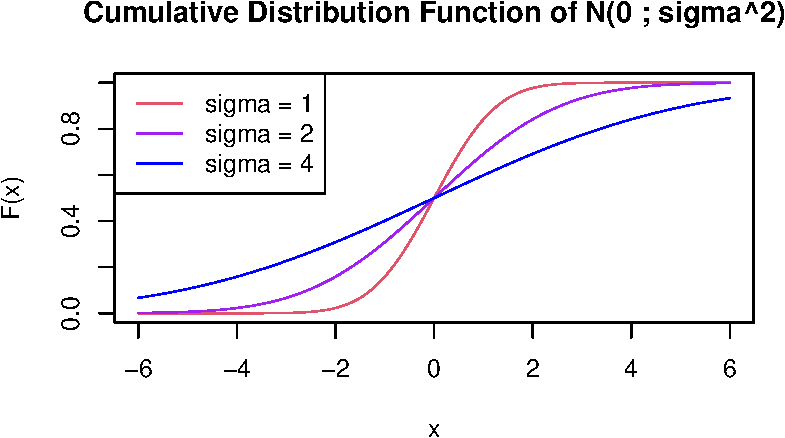
\includegraphics{051_distributions_unif_normal_files/figure-pdf/normalCum3-1.pdf}

We can also use \texttt{pnorm()}to verify the key property of the normal
distribution, that 68 \% of the values fall in between -1 and +1
standard deviation from the mean, and respectively 95\% and 98.7\% for 2
and 3 standard deviations.

\begin{Shaded}
\begin{Highlighting}[]
\DecValTok{1}\SpecialCharTok{{-}}\NormalTok{(}\FunctionTok{pnorm}\NormalTok{(}\SpecialCharTok{{-}}\DecValTok{1}\NormalTok{)}\SpecialCharTok{+}\NormalTok{(}\DecValTok{1}\SpecialCharTok{{-}}\FunctionTok{pnorm}\NormalTok{(}\DecValTok{1}\NormalTok{))) }\CommentTok{\#1 minus the sum of the probability of being below {-}1 and being above 1)}
\CommentTok{\#\textgreater{} [1] 0.6826895}
\FunctionTok{pnorm}\NormalTok{(}\DecValTok{1}\NormalTok{)}\SpecialCharTok{{-}}\FunctionTok{pnorm}\NormalTok{(}\SpecialCharTok{{-}}\DecValTok{1}\NormalTok{) }\CommentTok{\#or simply :{-}) }
\CommentTok{\#\textgreater{} [1] 0.6826895}

\DecValTok{1}\SpecialCharTok{{-}}\NormalTok{(}\FunctionTok{pnorm}\NormalTok{(}\SpecialCharTok{{-}}\DecValTok{2}\NormalTok{)}\SpecialCharTok{+}\NormalTok{(}\DecValTok{1}\SpecialCharTok{{-}}\FunctionTok{pnorm}\NormalTok{(}\DecValTok{2}\NormalTok{))) }
\CommentTok{\#\textgreater{} [1] 0.9544997}

\DecValTok{1}\SpecialCharTok{{-}}\NormalTok{(}\FunctionTok{pnorm}\NormalTok{(}\SpecialCharTok{{-}}\DecValTok{3}\NormalTok{)}\SpecialCharTok{+}\NormalTok{(}\DecValTok{1}\SpecialCharTok{{-}}\FunctionTok{pnorm}\NormalTok{(}\DecValTok{3}\NormalTok{))) }
\CommentTok{\#\textgreater{} [1] 0.9973002}
\end{Highlighting}
\end{Shaded}

Of course \texttt{pnorm()}can be interrogated for any normal
distribution, i.e.~with other means and standard deviations. For
example, suppose we know the mean of GDP /capita for all countries in
Europe is 40 000 euro on average with a standard deviation of 20 000 and
we have indication that the distribution is normal. What is the
probability of finding a country below the GDP of Latvia, i.e.~22 000
euro per capita or Luxembourg 100 000 euro per capita?

\begin{Shaded}
\begin{Highlighting}[]
\FunctionTok{pnorm}\NormalTok{(}\DecValTok{22000}\NormalTok{,}\AttributeTok{mean=}\DecValTok{40000}\NormalTok{,}\AttributeTok{sd =} \DecValTok{20000}\NormalTok{)}
\CommentTok{\#\textgreater{} [1] 0.1840601}
\FunctionTok{pnorm}\NormalTok{(}\DecValTok{100000}\NormalTok{,}\AttributeTok{mean=}\DecValTok{40000}\NormalTok{,}\AttributeTok{sd =} \DecValTok{20000}\NormalTok{)}
\CommentTok{\#\textgreater{} [1] 0.9986501}
\end{Highlighting}
\end{Shaded}

We see that about 18.4\% of the countries will have a GDP lower than
Latvia and 99.9\% will be lower than Luxembourg.

The other way around, we can ask what would be the GDP/capita for a
country to be in the top 1\% or top 10\% using \texttt{qnorm()}

\begin{Shaded}
\begin{Highlighting}[]
\FunctionTok{qnorm}\NormalTok{(}\FloatTok{0.99}\NormalTok{,}\AttributeTok{mean=}\DecValTok{40000}\NormalTok{,}\AttributeTok{sd =} \DecValTok{20000}\NormalTok{)}
\CommentTok{\#\textgreater{} [1] 86526.96}
\FunctionTok{qnorm}\NormalTok{(}\FloatTok{0.90}\NormalTok{,}\AttributeTok{mean=}\DecValTok{40000}\NormalTok{,}\AttributeTok{sd =} \DecValTok{20000}\NormalTok{)}
\CommentTok{\#\textgreater{} [1] 65631.03}
\FunctionTok{qnorm}\NormalTok{(}\FloatTok{0.5}\NormalTok{,}\AttributeTok{mean=}\DecValTok{40000}\NormalTok{,}\AttributeTok{sd =} \DecValTok{20000}\NormalTok{)}
\CommentTok{\#\textgreater{} [1] 40000}
\end{Highlighting}
\end{Shaded}

\chapter{Central Limit Theorem and
standardisation}\label{sec-central-limit-theorem-and-standardisation}

\section{Central Limit Theorem}\label{central-limit-theorem}

The reason for the success of the normal distribution is not only due to
its key features (symmetry and the linkage between quantiles and
standard deviations) but is also explained by the \textbf{Central Limit
Theorem}:

\begin{quote}
\textbf{\emph{If you take repeated samples from a population with finite
variance and calculate their averages, then the averages will be
normally distributed}} (Crawley (2012), p213)
\end{quote}

Let's draw 5 times a 100 numbers from a uniform distribution within the
interval 0 to 10. For each of the five cases, the average should be
close to 5.

\begin{Shaded}
\begin{Highlighting}[]
\FunctionTok{mean}\NormalTok{(}\FunctionTok{runif}\NormalTok{(}\DecValTok{100}\NormalTok{)}\SpecialCharTok{*}\DecValTok{10}\NormalTok{)}
\CommentTok{\#\textgreater{} [1] 5.249874}
\FunctionTok{mean}\NormalTok{(}\FunctionTok{runif}\NormalTok{(}\DecValTok{100}\NormalTok{)}\SpecialCharTok{*}\DecValTok{10}\NormalTok{)}
\CommentTok{\#\textgreater{} [1] 5.335763}
\FunctionTok{mean}\NormalTok{(}\FunctionTok{runif}\NormalTok{(}\DecValTok{100}\NormalTok{)}\SpecialCharTok{*}\DecValTok{10}\NormalTok{)}
\CommentTok{\#\textgreater{} [1] 4.871023}
\FunctionTok{mean}\NormalTok{(}\FunctionTok{runif}\NormalTok{(}\DecValTok{100}\NormalTok{)}\SpecialCharTok{*}\DecValTok{10}\NormalTok{)}
\CommentTok{\#\textgreater{} [1] 5.250669}
\FunctionTok{mean}\NormalTok{(}\FunctionTok{runif}\NormalTok{(}\DecValTok{100}\NormalTok{)}\SpecialCharTok{*}\DecValTok{10}\NormalTok{)}
\CommentTok{\#\textgreater{} [1] 4.868909}
\end{Highlighting}
\end{Shaded}

We can write this in a loop and produce a histogram of the means:

\begin{Shaded}
\begin{Highlighting}[]
\NormalTok{n}\OtherTok{\textless{}{-}}\DecValTok{5}
\NormalTok{means}\OtherTok{\textless{}{-}}\FunctionTok{numeric}\NormalTok{(n)}
\ControlFlowTok{for}\NormalTok{ (i }\ControlFlowTok{in} \DecValTok{1}\SpecialCharTok{:}\NormalTok{n)\{}
\NormalTok{  means[i]}\OtherTok{\textless{}{-}}\FunctionTok{mean}\NormalTok{(}\FunctionTok{runif}\NormalTok{(}\DecValTok{100}\NormalTok{)}\SpecialCharTok{*}\DecValTok{10}\NormalTok{)}
\NormalTok{\}}
\NormalTok{means}
\CommentTok{\#\textgreater{} [1] 4.828341 5.320251 5.058781 4.758916 5.185008}
\FunctionTok{hist}\NormalTok{(means)}
\end{Highlighting}
\end{Shaded}

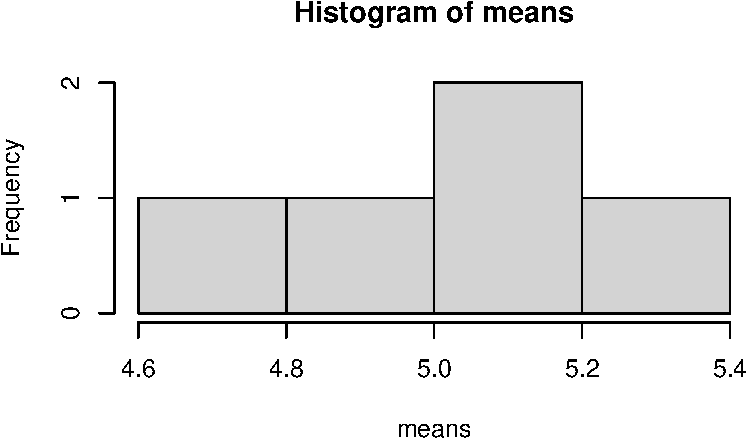
\includegraphics{052_CLT_Standardisation_files/figure-pdf/unnamed-chunk-2-1.pdf}

It is not quite impressive at this stage, but if we repeat, say 10000
times the experiment rather than 5, the histogram tends towards the
shape of a normal distribution!

\begin{Shaded}
\begin{Highlighting}[]
\NormalTok{n}\OtherTok{\textless{}{-}}\DecValTok{10000}
\NormalTok{means}\OtherTok{\textless{}{-}}\FunctionTok{numeric}\NormalTok{(n)}
\ControlFlowTok{for}\NormalTok{ (i }\ControlFlowTok{in} \DecValTok{1}\SpecialCharTok{:}\NormalTok{n)\{}
\NormalTok{  means[i]}\OtherTok{\textless{}{-}}\FunctionTok{mean}\NormalTok{(}\FunctionTok{runif}\NormalTok{(}\DecValTok{100}\NormalTok{)}\SpecialCharTok{*}\DecValTok{10}\NormalTok{)}
\NormalTok{\}}
\FunctionTok{head}\NormalTok{(means)}
\CommentTok{\#\textgreater{} [1] 4.704968 5.100424 4.725626 5.135044 5.060291 5.352029}
\FunctionTok{hist}\NormalTok{(means, }\AttributeTok{breaks=}\DecValTok{100}\NormalTok{)}
\end{Highlighting}
\end{Shaded}

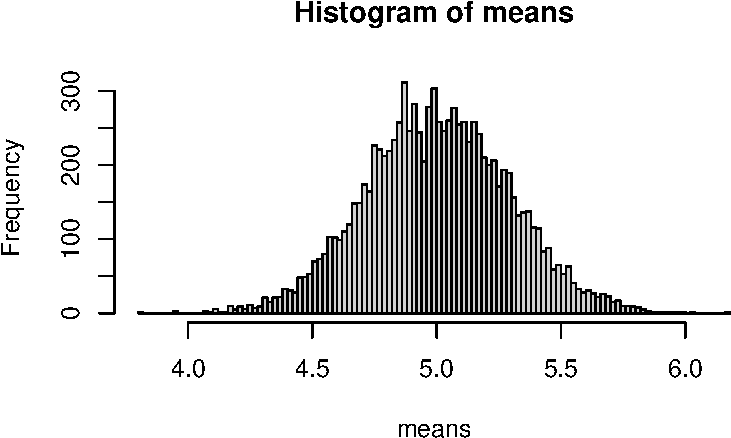
\includegraphics{052_CLT_Standardisation_files/figure-pdf/unnamed-chunk-3-1.pdf}

And the median, mean and standard deviation of the ``means'' are

\begin{Shaded}
\begin{Highlighting}[]
\FunctionTok{median}\NormalTok{(means)}
\CommentTok{\#\textgreater{} [1] 4.998585}
\FunctionTok{mean}\NormalTok{(means)}
\CommentTok{\#\textgreater{} [1] 5.001996}
\FunctionTok{sd}\NormalTok{(means)}
\CommentTok{\#\textgreater{} [1] 0.2901099}
\end{Highlighting}
\end{Shaded}

\section{Standardization}\label{standardization}

In order to visually appreciate how well the obtained distribution
compares to a corresponding normal distribution, we can generate a
normal distribution with the same parameters (mean and variance).
Alternatively, we can also \textbf{standardize} the outcome in order to
fit a ``Unit'' normal distribution, i.e.~one where the mean is 0 and the
standard deviation is 1.

This process is called \textbf{Standardization}. It involves
\textbf{centering} an empirical variable, i.e.~computing deviations to
the mean, so that the mean is set to 0, and \textbf{reducing} by
dividing the centered by the standard deviation. Hence making the new
standard deviation equal to 1. One often name a standradized variable Z.
The built in function for standardization is \texttt{scale()}. It
centers and reduces by default, but you can toggle one or the other on
or off.

Important: Since standardization involves a division by a number
(standard deviation) with the same units as the original variable,
\textbf{a standardized variable has no unit !} This is a property you
may like for comparing with other variables that have different original
units.

\begin{Shaded}
\begin{Highlighting}[]
\NormalTok{Centered}\OtherTok{\textless{}{-}}\NormalTok{means}\SpecialCharTok{{-}}\FunctionTok{mean}\NormalTok{(means) }\CommentTok{\#centering}
\NormalTok{Z}\OtherTok{\textless{}{-}}\NormalTok{Centered}\SpecialCharTok{/}\FunctionTok{sd}\NormalTok{(means) }\CommentTok{\#reducing /scaling}
\CommentTok{\#or simply }
\NormalTok{Z}\OtherTok{\textless{}{-}}\FunctionTok{scale}\NormalTok{(means, }\AttributeTok{center =} \ConstantTok{TRUE}\NormalTok{, }\AttributeTok{scale =} \ConstantTok{TRUE}\NormalTok{)}

\CommentTok{\#Compare}
\FunctionTok{cbind}\NormalTok{(}\FunctionTok{mean}\NormalTok{(means), }\FunctionTok{mean}\NormalTok{(Z))}
\CommentTok{\#\textgreater{}          [,1]         [,2]}
\CommentTok{\#\textgreater{} [1,] 5.001996 {-}9.61342e{-}16}
\FunctionTok{cbind}\NormalTok{(}\FunctionTok{sd}\NormalTok{(means), }\FunctionTok{sd}\NormalTok{(Z))}
\CommentTok{\#\textgreater{}           [,1] [,2]}
\CommentTok{\#\textgreater{} [1,] 0.2901099    1}
\end{Highlighting}
\end{Shaded}

\subsection{Standardized density from many
repetitions}\label{standardized-density-from-many-repetitions}

We can now compare our empirical distribution density (blue) to the
theoretical density of a unit normal distribution (black). The overlay
effectively proves the Central Limit Theorem, showing that even from a
very simple distribution like the uniform distribution, the mean over
repeated samples is distributed normally.

\begin{Shaded}
\begin{Highlighting}[]
\FunctionTok{curve}\NormalTok{(dnorm,}\SpecialCharTok{{-}}\DecValTok{4}\NormalTok{,}\DecValTok{4}\NormalTok{) }\CommentTok{\#Density of theoretical normal distribution}
\FunctionTok{lines}\NormalTok{(}\FunctionTok{density}\NormalTok{(Z), }\AttributeTok{col=}\StringTok{"blue"}\NormalTok{) }\CommentTok{\#Density of our empirical distribution after n repetitions}
\end{Highlighting}
\end{Shaded}

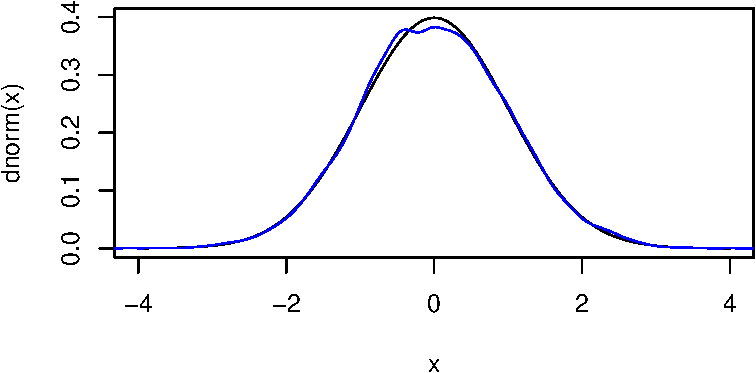
\includegraphics{052_CLT_Standardisation_files/figure-pdf/unnamed-chunk-6-1.pdf}

\subsection{QQplot}\label{qqplot-1}

Another classical way to know whether an empirical distribution
corresponds well to a given theoretical one is to use a
\textbf{quantile-quantile plot}, aka \textbf{qqplot}, where empirical
quantiles are plotted along the y-axis and theoretical ones
(e.g.~normal) along the x-axis.

We expect a straight line at least in a good range of values around the
mean. Towards the extreme there are less points and the variability is
thus greater. Given we look at the shape of the curve, not the values,
we don't need to standardize the data ahead this time (but of course
then the values on the two axes will differ). We verify visually that
the qqplot of our mean of means is close to a straight line.

\begin{Shaded}
\begin{Highlighting}[]
\FunctionTok{qqnorm}\NormalTok{(}\AttributeTok{y=}\NormalTok{means)}
\end{Highlighting}
\end{Shaded}

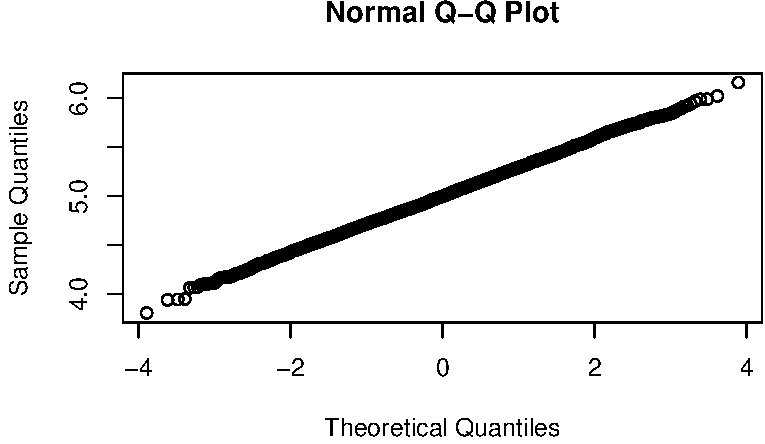
\includegraphics{052_CLT_Standardisation_files/figure-pdf/unnamed-chunk-7-1.pdf}

\chapter{Continuous distributions}\label{continuous-distributions}

In addition to the normal and uniform distributions, a number of other
continuous distributions are often used, corresponding to different
assumptions about the processes that shape the population.

\section{Exponential}\label{exponential}

A random variable \(X \in [0;+\infty[\) following an exponential
distribution with parameter \(\lambda > 0\) can be expressed as:
\(X \sim \epsilon(\lambda)\) with expectation \(E(X) = 1/ \lambda\) and
variance \(Var(X) = 1/ \lambda^2\).

Its \textbf{density function} can be written as:

\[f(x) = λ {e}^{- λ x} \text{ for } x \geq 0\]
\[f(x) = 0 \text{ for } x < 0\]

Its \textbf{cumulative distribution function} is defined by:

\[F_X(x) = 1 - \exp{(- \lambda x)} \text{ for } x \geq 0\]
\[F_X(x) = 0 \text{ for } x < 0\]

\begin{Shaded}
\begin{Highlighting}[]
\NormalTok{x }\OtherTok{\textless{}{-}} \FunctionTok{seq}\NormalTok{(}\DecValTok{0}\NormalTok{,}\DecValTok{8}\NormalTok{,}\FloatTok{0.01}\NormalTok{)}
\NormalTok{dExp}\FloatTok{.5} \OtherTok{\textless{}{-}} \FunctionTok{dexp}\NormalTok{(x, .}\DecValTok{5}\NormalTok{)}
\NormalTok{dExp1 }\OtherTok{\textless{}{-}} \FunctionTok{dexp}\NormalTok{(x, }\DecValTok{1}\NormalTok{)}
\NormalTok{dExp2 }\OtherTok{\textless{}{-}} \FunctionTok{dexp}\NormalTok{(x, }\DecValTok{2}\NormalTok{)}
\NormalTok{dExp3 }\OtherTok{\textless{}{-}} \FunctionTok{dexp}\NormalTok{(x, }\DecValTok{3}\NormalTok{)}
\end{Highlighting}
\end{Shaded}

\begin{Shaded}
\begin{Highlighting}[]
\FunctionTok{plot}\NormalTok{(x, dExp3, }\AttributeTok{type =} \StringTok{\textquotesingle{}l\textquotesingle{}}\NormalTok{, }\AttributeTok{col =} \StringTok{\textquotesingle{}green\textquotesingle{}}\NormalTok{,}
     \AttributeTok{main =} \StringTok{\textquotesingle{}Density function of X\textasciitilde{}Exp(lambda)\textquotesingle{}}\NormalTok{, }\AttributeTok{ylab =} \StringTok{\textquotesingle{}f(x)\textquotesingle{}}\NormalTok{)}
\FunctionTok{lines}\NormalTok{(x, dExp2, }\AttributeTok{col =} \StringTok{\textquotesingle{}gold\textquotesingle{}}\NormalTok{)}
\FunctionTok{lines}\NormalTok{(x, dExp1, }\AttributeTok{col =} \StringTok{\textquotesingle{}darkorange\textquotesingle{}}\NormalTok{)}
\FunctionTok{lines}\NormalTok{(x, dExp}\FloatTok{.5}\NormalTok{, }\AttributeTok{col =} \DecValTok{2}\NormalTok{)}
\FunctionTok{legend}\NormalTok{(}\StringTok{"topright"}\NormalTok{, }\AttributeTok{lty =} \DecValTok{1}\NormalTok{,}
       \AttributeTok{legend =} \FunctionTok{c}\NormalTok{(}\StringTok{"lambda = 0.5"}\NormalTok{, }\StringTok{"lambda = 1"}\NormalTok{, }
                  \StringTok{"lambda = 2"}\NormalTok{, }\StringTok{"lambda = 3"}\NormalTok{),}
       \AttributeTok{col =} \FunctionTok{c}\NormalTok{(}\DecValTok{2}\NormalTok{, }\StringTok{\textquotesingle{}darkorange\textquotesingle{}}\NormalTok{, }\StringTok{\textquotesingle{}gold\textquotesingle{}}\NormalTok{, }\StringTok{\textquotesingle{}green\textquotesingle{}}\NormalTok{))}
\end{Highlighting}
\end{Shaded}

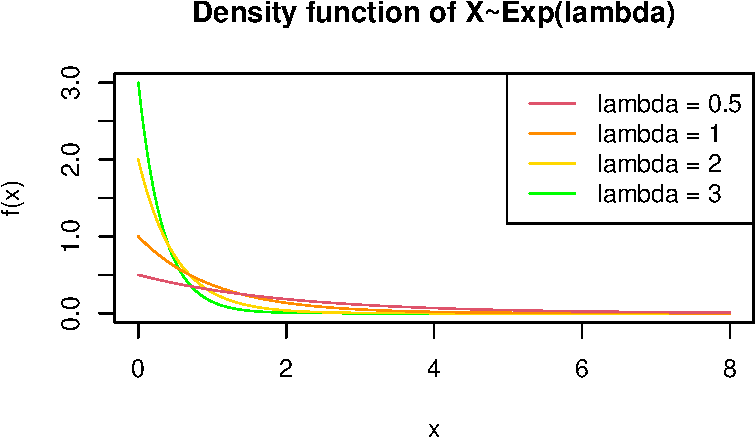
\includegraphics{053_distributions_other_continuous_files/figure-pdf/expDensity-1.pdf}

\begin{Shaded}
\begin{Highlighting}[]
\FunctionTok{plot}\NormalTok{(x, }\FunctionTok{pexp}\NormalTok{(x, }\DecValTok{3}\NormalTok{), }\AttributeTok{type =} \StringTok{\textquotesingle{}l\textquotesingle{}}\NormalTok{, }\AttributeTok{col =} \StringTok{\textquotesingle{}green\textquotesingle{}}\NormalTok{,}
     \AttributeTok{main =} \StringTok{\textquotesingle{}Cumulative Distribution Function of X\textasciitilde{}Exp(lambda)\textquotesingle{}}\NormalTok{, }\AttributeTok{ylab =} \StringTok{\textquotesingle{}F(x)\textquotesingle{}}\NormalTok{)}
\FunctionTok{lines}\NormalTok{(x, }\FunctionTok{pexp}\NormalTok{(x, }\DecValTok{2}\NormalTok{), }\AttributeTok{col=}\StringTok{\textquotesingle{}gold\textquotesingle{}}\NormalTok{)}
\FunctionTok{lines}\NormalTok{(x, }\FunctionTok{pexp}\NormalTok{(x, }\DecValTok{1}\NormalTok{), }\AttributeTok{col=}\StringTok{\textquotesingle{}darkorange\textquotesingle{}}\NormalTok{)}
\FunctionTok{lines}\NormalTok{(x, }\FunctionTok{pexp}\NormalTok{(x, .}\DecValTok{5}\NormalTok{), }\AttributeTok{col=}\DecValTok{2}\NormalTok{)}
\FunctionTok{legend}\NormalTok{(}\StringTok{"bottomright"}\NormalTok{, }\AttributeTok{lty =} \DecValTok{1}\NormalTok{,}
       \AttributeTok{legend =} \FunctionTok{c}\NormalTok{(}\StringTok{"lambda = 0.5"}\NormalTok{, }\StringTok{"lambda = 1"}\NormalTok{, }\StringTok{"lambda = 2"}\NormalTok{, }\StringTok{"lambda = 3"}\NormalTok{),}
       \AttributeTok{col =} \FunctionTok{c}\NormalTok{(}\DecValTok{2}\NormalTok{, }\StringTok{\textquotesingle{}darkorange\textquotesingle{}}\NormalTok{, }\StringTok{\textquotesingle{}gold\textquotesingle{}}\NormalTok{, }\StringTok{\textquotesingle{}green\textquotesingle{}}\NormalTok{))}
\end{Highlighting}
\end{Shaded}

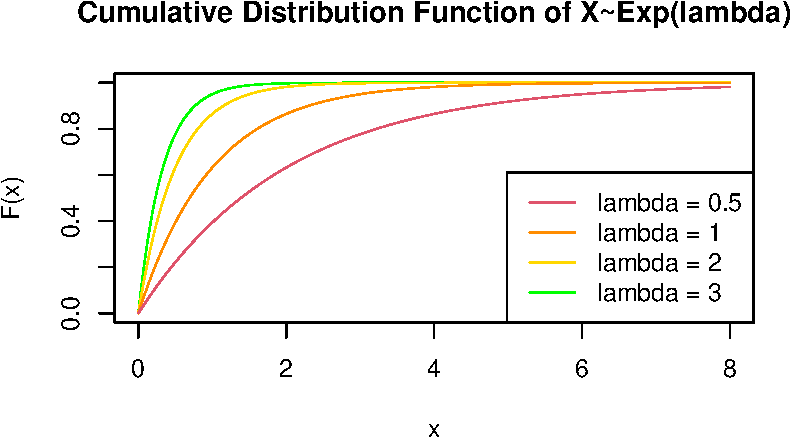
\includegraphics{053_distributions_other_continuous_files/figure-pdf/expCDF-1.pdf}

\section{Chi-square}\label{chi-square}

A random variable \(X\) following a chi-square (or khi-square)
distribution can be expressed as: \(X \sim \chi^2(k)\) with parameter
\(k> 0\), expectation \(E(X) = k\), variance \(Var(X) = 2k\).

\(k\) represents the degree of freedom.

The \textbf{density function} is

\[f_X(x) = \dfrac {1} {2^{k/2} \gamma(k/2)} x^{(k/2)-1} \exp{(\dfrac{-x}{2})} \text{ for } x \geq 0\]

\[f_X(x) = 0 \text{ for } x < 0\]

\begin{Shaded}
\begin{Highlighting}[]
\NormalTok{x }\OtherTok{\textless{}{-}} \FunctionTok{seq}\NormalTok{(}\DecValTok{0}\NormalTok{,}\DecValTok{8}\NormalTok{,}\FloatTok{0.01}\NormalTok{)}
\NormalTok{dChiSq1 }\OtherTok{\textless{}{-}} \FunctionTok{dchisq}\NormalTok{(x, }\AttributeTok{df=}\DecValTok{1}\NormalTok{)}
\NormalTok{dChiSq2 }\OtherTok{\textless{}{-}} \FunctionTok{dchisq}\NormalTok{(x, }\AttributeTok{df=}\DecValTok{2}\NormalTok{)}
\NormalTok{dChiSq3 }\OtherTok{\textless{}{-}} \FunctionTok{dchisq}\NormalTok{(x, }\AttributeTok{df=}\DecValTok{3}\NormalTok{)}
\NormalTok{dChiSq6 }\OtherTok{\textless{}{-}} \FunctionTok{dchisq}\NormalTok{(x, }\AttributeTok{df=}\DecValTok{6}\NormalTok{)}
\end{Highlighting}
\end{Shaded}

We see (and know from the CLT) that when the degrees of freedom
increases, the function gets closer to a normal distribution. However it
is not symmetrical and the right hand side stays longer than in the
normal distribution for quite some time.

\begin{Shaded}
\begin{Highlighting}[]
\FunctionTok{plot}\NormalTok{(x, dChiSq1, }\AttributeTok{type =} \StringTok{\textquotesingle{}l\textquotesingle{}}\NormalTok{, }\AttributeTok{col =} \DecValTok{2}\NormalTok{, }\AttributeTok{ylim =} \FunctionTok{c}\NormalTok{(}\DecValTok{0}\NormalTok{, }\FloatTok{1.25}\NormalTok{),}
     \AttributeTok{main =} \StringTok{\textquotesingle{}Density function of X\textasciitilde{}Chi\^{}2(p)\textquotesingle{}}\NormalTok{, }\AttributeTok{ylab =} \StringTok{\textquotesingle{}f(x)\textquotesingle{}}\NormalTok{)}
\FunctionTok{lines}\NormalTok{(x, dChiSq2, }\AttributeTok{col =} \StringTok{\textquotesingle{}darkorange\textquotesingle{}}\NormalTok{)}
\FunctionTok{lines}\NormalTok{(x, dChiSq3, }\AttributeTok{col =} \StringTok{\textquotesingle{}gold\textquotesingle{}}\NormalTok{)}
\FunctionTok{lines}\NormalTok{(x, dChiSq6, }\AttributeTok{col =} \StringTok{\textquotesingle{}green\textquotesingle{}}\NormalTok{)}
\FunctionTok{legend}\NormalTok{(}\StringTok{"topright"}\NormalTok{, }\AttributeTok{lty =} \DecValTok{1}\NormalTok{,}
       \AttributeTok{legend =} \FunctionTok{c}\NormalTok{(}\StringTok{"k = 1"}\NormalTok{, }\StringTok{"k = 2"}\NormalTok{, }\StringTok{"k = 3"}\NormalTok{, }\StringTok{"k = 6"}\NormalTok{),}
       \AttributeTok{col =} \FunctionTok{c}\NormalTok{(}\DecValTok{2}\NormalTok{, }\StringTok{\textquotesingle{}darkorange\textquotesingle{}}\NormalTok{, }\StringTok{\textquotesingle{}gold\textquotesingle{}}\NormalTok{, }\StringTok{\textquotesingle{}green\textquotesingle{}}\NormalTok{))}
\end{Highlighting}
\end{Shaded}

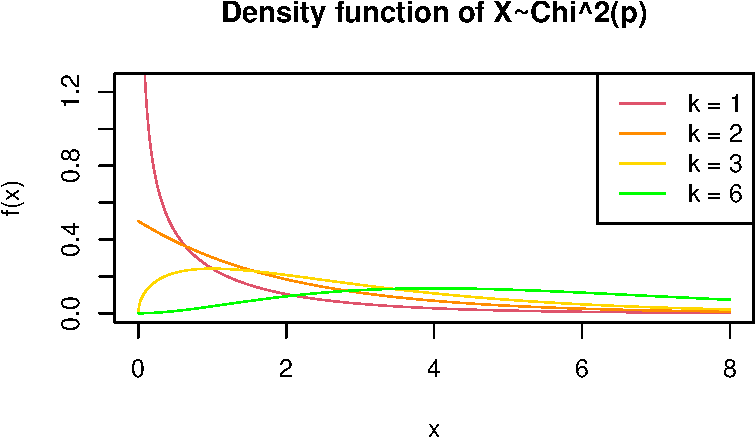
\includegraphics{053_distributions_other_continuous_files/figure-pdf/chi2Density-1.pdf}

The cumulative density is as follows:

\begin{Shaded}
\begin{Highlighting}[]
\FunctionTok{plot}\NormalTok{(x, }\FunctionTok{pchisq}\NormalTok{(x, }\AttributeTok{df=}\DecValTok{1}\NormalTok{), }\AttributeTok{type =} \StringTok{\textquotesingle{}l\textquotesingle{}}\NormalTok{, }\AttributeTok{col =} \DecValTok{2}\NormalTok{,}
     \AttributeTok{main =} \StringTok{\textquotesingle{}Cumulative Distribution Function of X\textasciitilde{}Chi2(p)\textquotesingle{}}\NormalTok{, }\AttributeTok{ylab =} \StringTok{\textquotesingle{}F(x)\textquotesingle{}}\NormalTok{)}
\FunctionTok{lines}\NormalTok{(x, }\FunctionTok{pchisq}\NormalTok{(x, }\AttributeTok{df=}\DecValTok{2}\NormalTok{), }\AttributeTok{col=}\StringTok{\textquotesingle{}darkorange\textquotesingle{}}\NormalTok{)}
\FunctionTok{lines}\NormalTok{(x, }\FunctionTok{pchisq}\NormalTok{(x, }\AttributeTok{df=}\DecValTok{3}\NormalTok{), }\AttributeTok{col=}\StringTok{\textquotesingle{}gold\textquotesingle{}}\NormalTok{)}
\FunctionTok{lines}\NormalTok{(x, }\FunctionTok{pchisq}\NormalTok{(x, }\AttributeTok{df=}\DecValTok{6}\NormalTok{), }\AttributeTok{col=}\StringTok{\textquotesingle{}green\textquotesingle{}}\NormalTok{)}
\FunctionTok{legend}\NormalTok{(}\StringTok{"bottomright"}\NormalTok{, }\AttributeTok{lty =} \DecValTok{1}\NormalTok{,}
       \AttributeTok{legend =} \FunctionTok{c}\NormalTok{(}\StringTok{"k = 1"}\NormalTok{, }\StringTok{"k = 2"}\NormalTok{, }\StringTok{"k = 3"}\NormalTok{, }\StringTok{"k = 6"}\NormalTok{),}
       \AttributeTok{col =} \FunctionTok{c}\NormalTok{(}\DecValTok{2}\NormalTok{, }\StringTok{\textquotesingle{}darkorange\textquotesingle{}}\NormalTok{, }\StringTok{\textquotesingle{}gold\textquotesingle{}}\NormalTok{, }\StringTok{\textquotesingle{}green\textquotesingle{}}\NormalTok{))}
\end{Highlighting}
\end{Shaded}

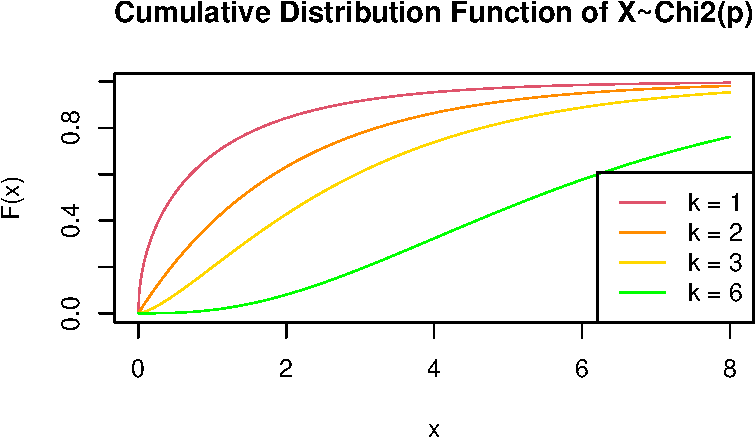
\includegraphics{053_distributions_other_continuous_files/figure-pdf/chi2CDF-1.pdf}

The chi-square distribution is typically used to test the independence
of two variables. It is typically applied to a categorical or ordinal
metric along two categories, e.g.~the level of education of Luxembourg
natives vs Luxembourg migrants or the counts of votes for Kamala Harris
among young vs elders population or among urban vs rural population. It
is thus often applied to contingency tables after the cross-tabulation
of two factors in order to test if observed frequencies differ from
expected frequencies.

The df considered are usually low since it corresponds to the number of
categories-1 (e.g.~urban+rural, i.e.~2 -1=1) times the types of output
-1, (e.g.~vote for Harris vs Trump, i.e.~2-1=1). Thus far from a normal
distribution.

\section{Student t-distribution}\label{student-t-distribution}

A random variable \(X\) following a student distribution, can be
expressed as: \(X \sim t(n)\) with parameter \(n\) degrees of freedom.

Its \textbf{density function} is

\[f(x) = \dfrac{1}{\sqrt{n\pi}} \dfrac {\gamma{(\dfrac{n+1}{2})}} {\gamma{(\dfrac{n}{2})}} \dfrac {1} {(1+\dfrac{x^2}{n})^{(n+1)/2}} \text{ for all } x\in R\]
We have: \[E(X) = 0 \text{ for } n \ge 2\]
\[Var(X) = \dfrac{n}{n-2} \text{ for } n \ge 3\]

If we have a random variable \(U \sim N (0, 1)\) and a random variable
\(X \sim \chi^2(n)\) which are independent, then the random variable
\(T_n = \dfrac{U}{\sqrt{X/n}}\) follows a student distribution \(t(n)\)

\begin{Shaded}
\begin{Highlighting}[]
\NormalTok{x }\OtherTok{\textless{}{-}} \FunctionTok{seq}\NormalTok{(}\SpecialCharTok{{-}}\DecValTok{8}\NormalTok{, }\DecValTok{8}\NormalTok{, }\FloatTok{0.01}\NormalTok{)}
\NormalTok{dStudent1 }\OtherTok{\textless{}{-}} \FunctionTok{dt}\NormalTok{(x, }\DecValTok{1}\NormalTok{)}
\NormalTok{dStudent2 }\OtherTok{\textless{}{-}} \FunctionTok{dt}\NormalTok{(x, }\DecValTok{2}\NormalTok{)}
\NormalTok{dStudent4 }\OtherTok{\textless{}{-}} \FunctionTok{dt}\NormalTok{(x, }\DecValTok{4}\NormalTok{)}
\end{Highlighting}
\end{Shaded}

\begin{Shaded}
\begin{Highlighting}[]
\FunctionTok{plot}\NormalTok{(x, }\FunctionTok{dnorm}\NormalTok{(x), }\AttributeTok{type =} \StringTok{\textquotesingle{}l\textquotesingle{}}\NormalTok{, }\AttributeTok{col =} \StringTok{\textquotesingle{}darkgray\textquotesingle{}}\NormalTok{, }\AttributeTok{xlim =} \FunctionTok{c}\NormalTok{(}\SpecialCharTok{{-}}\DecValTok{4}\NormalTok{, }\DecValTok{4}\NormalTok{), }\AttributeTok{lty =} \DecValTok{3}\NormalTok{,}
     \AttributeTok{main =} \StringTok{\textquotesingle{}Density function of X\textasciitilde{}t(n)\textquotesingle{}}\NormalTok{, }\AttributeTok{ylab =} \StringTok{\textquotesingle{}f(x)\textquotesingle{}}\NormalTok{)}
\FunctionTok{lines}\NormalTok{(x, dStudent4, }\AttributeTok{col =} \StringTok{\textquotesingle{}gold\textquotesingle{}}\NormalTok{)}
\FunctionTok{lines}\NormalTok{(x, dStudent2, }\AttributeTok{col =} \StringTok{\textquotesingle{}darkorange\textquotesingle{}}\NormalTok{)}
\FunctionTok{lines}\NormalTok{(x, dStudent1, }\AttributeTok{col =} \DecValTok{2}\NormalTok{)}
\FunctionTok{legend}\NormalTok{(}\StringTok{"topright"}\NormalTok{, }\AttributeTok{lty =} \FunctionTok{c}\NormalTok{(}\FunctionTok{rep}\NormalTok{(}\DecValTok{1}\NormalTok{, }\DecValTok{3}\NormalTok{), }\DecValTok{3}\NormalTok{),}
       \AttributeTok{legend =} \FunctionTok{c}\NormalTok{(}\StringTok{"t(n = 1)"}\NormalTok{, }\StringTok{"t(n = 2)"}\NormalTok{, }\StringTok{"t(n = 4)"}\NormalTok{, }\StringTok{"N(0,1)"}\NormalTok{),}
       \AttributeTok{col =} \FunctionTok{c}\NormalTok{(}\DecValTok{2}\NormalTok{, }\StringTok{\textquotesingle{}darkorange\textquotesingle{}}\NormalTok{, }\StringTok{\textquotesingle{}gold\textquotesingle{}}\NormalTok{, }\StringTok{\textquotesingle{}darkgray\textquotesingle{}}\NormalTok{))}
\end{Highlighting}
\end{Shaded}

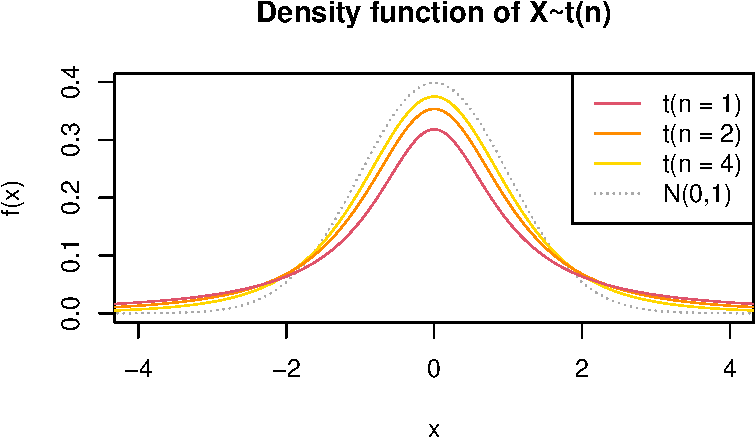
\includegraphics{053_distributions_other_continuous_files/figure-pdf/studentDensity-1.pdf}

\begin{Shaded}
\begin{Highlighting}[]
\FunctionTok{plot}\NormalTok{(x, }\FunctionTok{pnorm}\NormalTok{(x), }\AttributeTok{type =} \StringTok{\textquotesingle{}l\textquotesingle{}}\NormalTok{, }\AttributeTok{col =} \StringTok{\textquotesingle{}darkgray\textquotesingle{}}\NormalTok{, }\AttributeTok{lty =} \DecValTok{3}\NormalTok{,}
     \AttributeTok{main =} \StringTok{\textquotesingle{}Cumulative Distribution Function of X\textasciitilde{}t(n)\textquotesingle{}}\NormalTok{, }\AttributeTok{ylab =} \StringTok{\textquotesingle{}F(x)\textquotesingle{}}\NormalTok{)}
\FunctionTok{lines}\NormalTok{(x, }\FunctionTok{pt}\NormalTok{(x, }\DecValTok{2}\NormalTok{), }\AttributeTok{col=}\StringTok{\textquotesingle{}gold\textquotesingle{}}\NormalTok{)}
\FunctionTok{lines}\NormalTok{(x, }\FunctionTok{pt}\NormalTok{(x, }\DecValTok{3}\NormalTok{), }\AttributeTok{col=}\StringTok{\textquotesingle{}darkorange\textquotesingle{}}\NormalTok{)}
\FunctionTok{lines}\NormalTok{(x, }\FunctionTok{pt}\NormalTok{(x, }\DecValTok{6}\NormalTok{), }\AttributeTok{col=}\DecValTok{2}\NormalTok{)}
\FunctionTok{legend}\NormalTok{(}\StringTok{"bottomright"}\NormalTok{, }\AttributeTok{lty =} \FunctionTok{c}\NormalTok{(}\FunctionTok{rep}\NormalTok{(}\DecValTok{1}\NormalTok{, }\DecValTok{3}\NormalTok{), }\DecValTok{3}\NormalTok{),}
       \AttributeTok{legend =} \FunctionTok{c}\NormalTok{(}\StringTok{"t(n = 1)"}\NormalTok{, }\StringTok{"t(n = 2)"}\NormalTok{, }\StringTok{"t(n = 4)"}\NormalTok{, }\StringTok{"N(0,1)"}\NormalTok{),}
       \AttributeTok{col =} \FunctionTok{c}\NormalTok{(}\DecValTok{2}\NormalTok{, }\StringTok{\textquotesingle{}darkorange\textquotesingle{}}\NormalTok{, }\StringTok{\textquotesingle{}gold\textquotesingle{}}\NormalTok{, }\StringTok{\textquotesingle{}darkgray\textquotesingle{}}\NormalTok{))}
\end{Highlighting}
\end{Shaded}

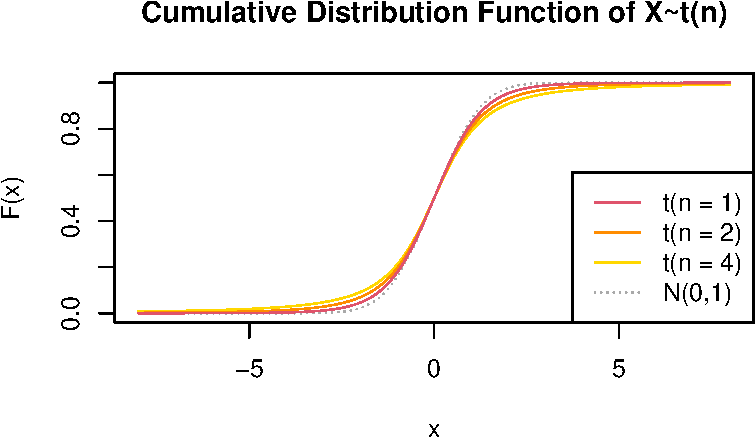
\includegraphics{053_distributions_other_continuous_files/figure-pdf/studentCDF-1.pdf}

Compared to the normal distribution, we can see the t-distribution
depends solely on \(n\). It is used for continuous variables in the
non-rare cases where the sample size is small and the variance of the
population is unknown.

t-Student's tests are typically used to test whether two samples have
different means or if a sample mean differ from a given value.

\section{Fisher-Snedecor}\label{fisher-snedecor}

A random variable \(X\) following a Fisher-Snedecor distribution can be
expressed as \(X \sim F(n, p)\) with parameters \(n\) and \(p\) degrees
of freedom.

Its \textbf{density function} is

\[f_X(x) = \dfrac {\gamma(\dfrac{n+p}{2})} {\gamma(\dfrac{n}{2}) \gamma(\dfrac{p}{2})} (\dfrac{n}{p})^{(n/2)} \dfrac{x^{\dfrac{n-2}{2}}}{(1 + \dfrac{n}{p}x)^{\dfrac{n-2}{2}}} \text{ for } x \geq 0\]
\[f_X(x) = 0 \text{ for } x < 0\]

We have:

\[E(X) = \dfrac{p}{p-2} \text{ for } p \ge 3\]
\[Var(X) = \dfrac{2p^2(n+p-2)}{n(p-2)^2(p-4)} \text{ for } p \ge 5\]

If we have two random variables \(X\) and \(Y\) independent such that
\(X \sim \chi^2(n)\) and \(Y \sim \chi^2(p)\), then the random variable
\(\dfrac{X/n}{Y/p}\) follows a Fisher distribution \(F(n, p)\)

\begin{Shaded}
\begin{Highlighting}[]
\NormalTok{x }\OtherTok{\textless{}{-}} \FunctionTok{seq}\NormalTok{(}\DecValTok{0}\NormalTok{, }\DecValTok{3}\NormalTok{, }\FloatTok{0.01}\NormalTok{)}
\NormalTok{dF1 }\OtherTok{\textless{}{-}} \FunctionTok{df}\NormalTok{(x, }\DecValTok{1}\NormalTok{, }\DecValTok{1}\NormalTok{)}
\NormalTok{dF10 }\OtherTok{\textless{}{-}} \FunctionTok{df}\NormalTok{(x, }\DecValTok{10}\NormalTok{, }\DecValTok{10}\NormalTok{)}
\NormalTok{dF20 }\OtherTok{\textless{}{-}} \FunctionTok{df}\NormalTok{(x, }\DecValTok{20}\NormalTok{, }\DecValTok{20}\NormalTok{)}
\NormalTok{dF50 }\OtherTok{\textless{}{-}} \FunctionTok{df}\NormalTok{(x, }\DecValTok{50}\NormalTok{, }\DecValTok{50}\NormalTok{)}
\end{Highlighting}
\end{Shaded}

\begin{Shaded}
\begin{Highlighting}[]
\FunctionTok{plot}\NormalTok{(x, dF1, }\AttributeTok{type =} \StringTok{\textquotesingle{}l\textquotesingle{}}\NormalTok{, }\AttributeTok{col =} \DecValTok{2}\NormalTok{, }
     \AttributeTok{main =} \StringTok{\textquotesingle{}Density function of X \textasciitilde{} F(n, p)\textquotesingle{}}\NormalTok{, }\AttributeTok{ylab =} \StringTok{\textquotesingle{}f(x)\textquotesingle{}}\NormalTok{)}
\FunctionTok{lines}\NormalTok{(x, dF10, }\AttributeTok{col =} \StringTok{\textquotesingle{}darkorange\textquotesingle{}}\NormalTok{)}
\FunctionTok{lines}\NormalTok{(x, dF20, }\AttributeTok{col =} \StringTok{\textquotesingle{}gold\textquotesingle{}}\NormalTok{)}
\FunctionTok{lines}\NormalTok{(x, dF50, }\AttributeTok{col =} \StringTok{\textquotesingle{}green\textquotesingle{}}\NormalTok{)}
\FunctionTok{legend}\NormalTok{(}\StringTok{"topright"}\NormalTok{, }\AttributeTok{lty =} \DecValTok{1}\NormalTok{,}
       \AttributeTok{legend =} \FunctionTok{c}\NormalTok{(}\StringTok{"F(n = p = 1)"}\NormalTok{, }\StringTok{"F(n = p = 10)"}\NormalTok{, }\StringTok{"F(n = p = 20)"}\NormalTok{, }\StringTok{"F(n = p = 50)"}\NormalTok{),}
       \AttributeTok{col =} \FunctionTok{c}\NormalTok{(}\DecValTok{2}\NormalTok{, }\StringTok{\textquotesingle{}darkorange\textquotesingle{}}\NormalTok{, }\StringTok{\textquotesingle{}gold\textquotesingle{}}\NormalTok{, }\StringTok{\textquotesingle{}green\textquotesingle{}}\NormalTok{))}
\end{Highlighting}
\end{Shaded}

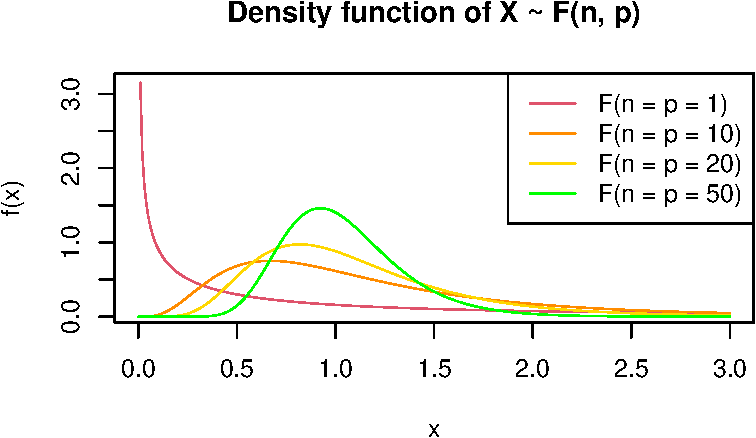
\includegraphics{053_distributions_other_continuous_files/figure-pdf/fisherDensity-1.pdf}

\begin{Shaded}
\begin{Highlighting}[]
\FunctionTok{plot}\NormalTok{(x, }\FunctionTok{pf}\NormalTok{(x, }\DecValTok{50}\NormalTok{, }\DecValTok{50}\NormalTok{), }\AttributeTok{type =} \StringTok{\textquotesingle{}l\textquotesingle{}}\NormalTok{, }\AttributeTok{col =} \StringTok{\textquotesingle{}green\textquotesingle{}}\NormalTok{,}
     \AttributeTok{main =} \StringTok{\textquotesingle{}Cumulative Distribution Function of X \textasciitilde{} F(n, p)\textquotesingle{}}\NormalTok{, }\AttributeTok{ylab =} \StringTok{\textquotesingle{}F(x)\textquotesingle{}}\NormalTok{)}
\FunctionTok{lines}\NormalTok{(x, }\FunctionTok{pf}\NormalTok{(x, }\DecValTok{20}\NormalTok{, }\DecValTok{20}\NormalTok{), }\AttributeTok{col=}\StringTok{\textquotesingle{}gold\textquotesingle{}}\NormalTok{)}
\FunctionTok{lines}\NormalTok{(x, }\FunctionTok{pf}\NormalTok{(x, }\DecValTok{10}\NormalTok{, }\DecValTok{10}\NormalTok{), }\AttributeTok{col=}\StringTok{\textquotesingle{}darkorange\textquotesingle{}}\NormalTok{)}
\FunctionTok{lines}\NormalTok{(x, }\FunctionTok{pf}\NormalTok{(x, }\DecValTok{1}\NormalTok{, }\DecValTok{1}\NormalTok{), }\AttributeTok{col=}\DecValTok{2}\NormalTok{)}
\FunctionTok{legend}\NormalTok{(}\StringTok{"bottomright"}\NormalTok{, }\AttributeTok{lty =} \DecValTok{1}\NormalTok{,}
       \AttributeTok{legend =} \FunctionTok{c}\NormalTok{(}\StringTok{"F(n = p = 1)"}\NormalTok{, }\StringTok{"F(n = p = 10)"}\NormalTok{, }\StringTok{"F(n = p = 20)"}\NormalTok{, }\StringTok{"F(n = p = 50)"}\NormalTok{),}
       \AttributeTok{col =} \FunctionTok{c}\NormalTok{(}\DecValTok{2}\NormalTok{, }\StringTok{\textquotesingle{}darkorange\textquotesingle{}}\NormalTok{, }\StringTok{\textquotesingle{}gold\textquotesingle{}}\NormalTok{, }\StringTok{\textquotesingle{}green\textquotesingle{}}\NormalTok{))}
\end{Highlighting}
\end{Shaded}

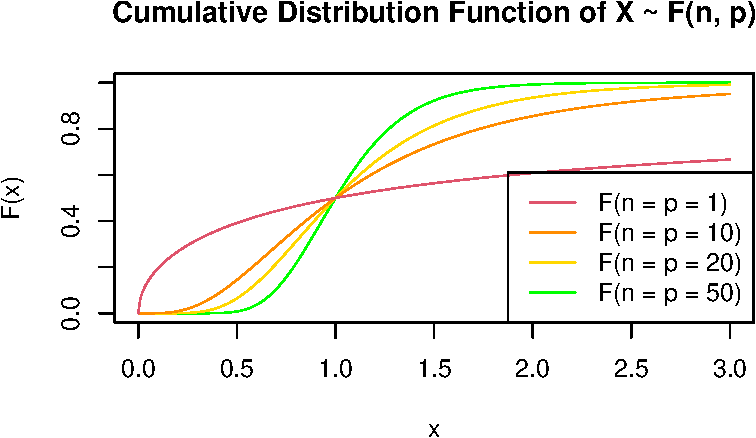
\includegraphics{053_distributions_other_continuous_files/figure-pdf/fisherCDF-1.pdf}

You will mostly encounter F-tests in association with the goodness of
fit of a regression analysis. It is used to test whether a linear model
better fits the data than a `intercept only' model, i.e.~one that
contains no independent variables, i.e.~whether your model provides any
useful information for prediction.

\chapter{Discrete distributions}\label{discrete-distributions}

\section{Discrete uniform
distribution}\label{discrete-uniform-distribution}

(to be done)

\section{Discrete binomial
distribution}\label{discrete-binomial-distribution}

Throwing a coin holds two possible values and generates a so called
Bernoulli random variable. We can represent the outcome by a 0 or 1.
Let's suppose 1 (whichever side you choose) is what we consider a
success. This is the usual convention.

A binomial distribution is the sum of independent and identically
distributed Bernoulli random variables.

When there are \(n\) Bernoulli trials (all independent), then the sum of
those trials, each with the same probability of success \(p\)) is
binomially distributed, with parameters \(n\) and \(p\). It is defined
with the two parameters: \(B(n, p)\) with parameter \(p \in [0; 1]\),
the probability that the event of interest (success) happens

A Bernoulli random variable \(X = \{0 ;1\}\) can thus be expressed as a
binomial distribution with a single toss \(n=1\), \(X \sim B(1, p)\)

\begin{verbatim}
    X        1         0
-------- --------- ---------
$P(X=i)$    $p$    $q = 1-p$
\end{verbatim}

The probability that \(X\) takes any other value is null (unless the
coin stays on its edge\ldots)

In a binomial distribution, the expectation is \(E(X) = np\) and the
variance is \(Var(X) = npq\).

The probability that one obtains \(k\) successes over \(n\) repetitions
(experiences), is then given by \(P(X=k) = (n|k) p^k q^{n-k}\).

For an intuition we can simulate 3 trials and produce a tree of
probabilities. Where we see that the probability of 3 successes is one
of 8 possible outcomes,

\begin{verbatim}
     1st      2nd     3rd         Total
     result   result  result
     
                     --1--        3 successes
              --1---|
             |       --0--        2 successes
     --1-----|
    |        |       --1--        2 successes
    |         --0---|
    |                --0--        1 success
----|
    |                --1--        2 successes
    |         --1---|
    |        |       --0--        1 success
     --0-----|
             |       --1--        1 success
              --0---|
                     --0--        0 success
\end{verbatim}

which in R is:

\begin{Shaded}
\begin{Highlighting}[]
\FunctionTok{dbinom}\NormalTok{(}\DecValTok{3}\NormalTok{, }\AttributeTok{size=}\DecValTok{3}\NormalTok{, }\AttributeTok{prob=}\FloatTok{0.5}\NormalTok{)}
\CommentTok{\#\textgreater{} [1] 0.125}
\end{Highlighting}
\end{Shaded}

Other example: suppose we run a trial 10 times, knowing the probability
of success is 0.5, what is the probability that the total number of
successes will be exactly 3? or exactly 5 ? or 10?

\begin{Shaded}
\begin{Highlighting}[]
\FunctionTok{dbinom}\NormalTok{(}\DecValTok{3}\NormalTok{, }\AttributeTok{size=}\DecValTok{10}\NormalTok{, }\AttributeTok{prob=}\FloatTok{0.5}\NormalTok{)}
\CommentTok{\#\textgreater{} [1] 0.1171875}
\FunctionTok{dbinom}\NormalTok{(}\DecValTok{5}\NormalTok{, }\AttributeTok{size=}\DecValTok{10}\NormalTok{, }\AttributeTok{prob=}\FloatTok{0.5}\NormalTok{)}
\CommentTok{\#\textgreater{} [1] 0.2460938}
\FunctionTok{dbinom}\NormalTok{(}\DecValTok{10}\NormalTok{, }\AttributeTok{size=}\DecValTok{10}\NormalTok{, }\AttributeTok{prob=}\FloatTok{0.5}\NormalTok{)}
\CommentTok{\#\textgreater{} [1] 0.0009765625}
\end{Highlighting}
\end{Shaded}

Let's generalize a little for values from 1 to 100 and different
probabilities:

\begin{Shaded}
\begin{Highlighting}[]
\NormalTok{x }\OtherTok{\textless{}{-}} \DecValTok{1}\SpecialCharTok{:}\DecValTok{100}
\NormalTok{dBer1 }\OtherTok{\textless{}{-}} \FunctionTok{dbinom}\NormalTok{(x, }\AttributeTok{size=}\DecValTok{100}\NormalTok{, }\AttributeTok{prob=}\FloatTok{0.1}\NormalTok{)}
\NormalTok{dBer2 }\OtherTok{\textless{}{-}} \FunctionTok{dbinom}\NormalTok{(x, }\AttributeTok{size=}\DecValTok{100}\NormalTok{, }\AttributeTok{prob=}\FloatTok{0.25}\NormalTok{)}
\NormalTok{dBer3 }\OtherTok{\textless{}{-}} \FunctionTok{dbinom}\NormalTok{(x, }\AttributeTok{size=}\DecValTok{100}\NormalTok{, }\AttributeTok{prob=}\FloatTok{0.5}\NormalTok{)}
\NormalTok{dBer4 }\OtherTok{\textless{}{-}} \FunctionTok{dbinom}\NormalTok{(x, }\AttributeTok{size=}\DecValTok{100}\NormalTok{, }\AttributeTok{prob=}\FloatTok{0.75}\NormalTok{)}
\NormalTok{dBer5 }\OtherTok{\textless{}{-}} \FunctionTok{dbinom}\NormalTok{(x, }\AttributeTok{size=}\DecValTok{100}\NormalTok{, }\AttributeTok{prob=}\FloatTok{0.9}\NormalTok{)}
\end{Highlighting}
\end{Shaded}

With 100 trials, you can see the density `curve' is symmetrical but
shifted towards higher total success when the probability of success
gets higher, and is flatter when closer to 0.5, (and symmetrical
behaviour for cases for \(p\) and \(q=1-p\))

\begin{Shaded}
\begin{Highlighting}[]
\FunctionTok{plot}\NormalTok{(x, dBer1,}\AttributeTok{main =} \StringTok{\textquotesingle{}Distribution of B(100, p)\textquotesingle{}}\NormalTok{, }\AttributeTok{ylab =} \StringTok{\textquotesingle{}f(x)\textquotesingle{}}\NormalTok{, }\AttributeTok{type=}\StringTok{"h"}\NormalTok{, }\AttributeTok{col =} \StringTok{\textquotesingle{}darkgreen\textquotesingle{}}\NormalTok{)}
\FunctionTok{points}\NormalTok{(x, dBer2, }\AttributeTok{col =} \StringTok{\textquotesingle{}lightgreen\textquotesingle{}}\NormalTok{, }\AttributeTok{type=}\StringTok{"h"}\NormalTok{)}
\FunctionTok{points}\NormalTok{(x, dBer3, }\AttributeTok{col =} \StringTok{\textquotesingle{}gold\textquotesingle{}}\NormalTok{, }\AttributeTok{type=}\StringTok{"h"}\NormalTok{)}
\FunctionTok{points}\NormalTok{(x, dBer4, }\AttributeTok{col =} \StringTok{\textquotesingle{}orange\textquotesingle{}}\NormalTok{, }\AttributeTok{type=}\StringTok{"h"}\NormalTok{)}
\FunctionTok{points}\NormalTok{(x, dBer5, }\AttributeTok{col =} \StringTok{\textquotesingle{}darkred\textquotesingle{}}\NormalTok{, }\AttributeTok{type=}\StringTok{"h"}\NormalTok{)}
\FunctionTok{legend}\NormalTok{(}\StringTok{"top"}\NormalTok{,}\AttributeTok{pch=}\DecValTok{1}\NormalTok{,}
       \AttributeTok{legend =} \FunctionTok{c}\NormalTok{(}\StringTok{"p = 0.10"}\NormalTok{, }\StringTok{"p = 0.25"}\NormalTok{, }\StringTok{"p = 0.50"}\NormalTok{,}\StringTok{"p = 0.75"}\NormalTok{, }\StringTok{"p = 0.90"}\NormalTok{),}
       \AttributeTok{col =} \FunctionTok{c}\NormalTok{(}\StringTok{"darkgreen"}\NormalTok{,}\StringTok{"lightgreen"}\NormalTok{, }\StringTok{\textquotesingle{}gold\textquotesingle{}}\NormalTok{, }\StringTok{\textquotesingle{}orange\textquotesingle{}}\NormalTok{,}\StringTok{"darkred"}\NormalTok{))}
\end{Highlighting}
\end{Shaded}

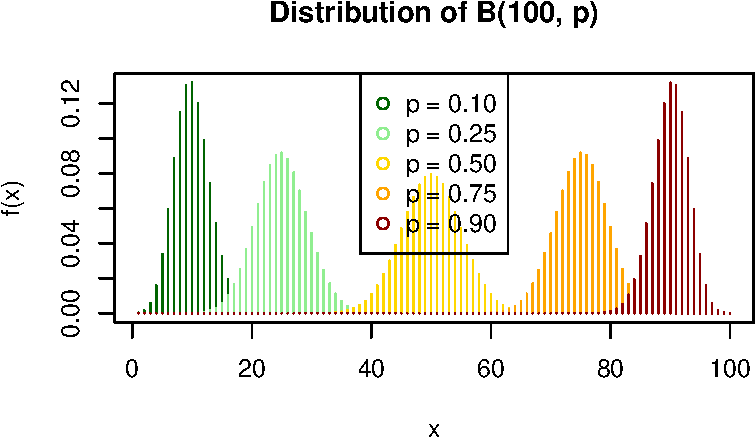
\includegraphics{054_distributions_discrete_files/figure-pdf/unnamed-chunk-4-1.pdf}

Back to using \(p=0.5\), we now look at the effect of sample size to see
how from right-skewed it shifts to a normal distribution:

\begin{Shaded}
\begin{Highlighting}[]
\NormalTok{dn1 }\OtherTok{\textless{}{-}} \FunctionTok{dbinom}\NormalTok{(x, }\AttributeTok{size=}\DecValTok{5}\NormalTok{, }\AttributeTok{prob=}\FloatTok{0.5}\NormalTok{)}
\NormalTok{dn2 }\OtherTok{\textless{}{-}} \FunctionTok{dbinom}\NormalTok{(x, }\AttributeTok{size=}\DecValTok{10}\NormalTok{, }\AttributeTok{prob=}\FloatTok{0.5}\NormalTok{)}
\NormalTok{dn3 }\OtherTok{\textless{}{-}} \FunctionTok{dbinom}\NormalTok{(x, }\AttributeTok{size=}\DecValTok{50}\NormalTok{, }\AttributeTok{prob=}\FloatTok{0.5}\NormalTok{)}
\NormalTok{dn4 }\OtherTok{\textless{}{-}} \FunctionTok{dbinom}\NormalTok{(x, }\AttributeTok{size=}\DecValTok{100}\NormalTok{, }\AttributeTok{prob=}\FloatTok{0.5}\NormalTok{)}
\end{Highlighting}
\end{Shaded}

\begin{Shaded}
\begin{Highlighting}[]
\FunctionTok{plot}\NormalTok{(x, dn1, }\AttributeTok{col=}\StringTok{"lightblue"}\NormalTok{, }\AttributeTok{type=}\StringTok{"h"}\NormalTok{,}
     \AttributeTok{main =} \StringTok{\textquotesingle{}Distribution of B(n, 0.5)\textquotesingle{}}\NormalTok{, }\AttributeTok{ylab =} \StringTok{\textquotesingle{}f(x)\textquotesingle{}}\NormalTok{)}
\FunctionTok{points}\NormalTok{(x, dn2, }\AttributeTok{col =} \StringTok{\textquotesingle{}blue\textquotesingle{}}\NormalTok{, }\AttributeTok{type=}\StringTok{"h"}\NormalTok{)}
\FunctionTok{points}\NormalTok{(x, dn3, }\AttributeTok{col =} \StringTok{\textquotesingle{}blue4\textquotesingle{}}\NormalTok{, }\AttributeTok{type=}\StringTok{"h"}\NormalTok{)}
\FunctionTok{points}\NormalTok{(x, dn4, }\AttributeTok{col =} \StringTok{\textquotesingle{}purple\textquotesingle{}}\NormalTok{,  }\AttributeTok{type=}\StringTok{"h"}\NormalTok{)}
\FunctionTok{legend}\NormalTok{(}\StringTok{"top"}\NormalTok{, }\AttributeTok{pch =} \DecValTok{1}\NormalTok{,}
       \AttributeTok{legend =} \FunctionTok{c}\NormalTok{(}\StringTok{"n = 5"}\NormalTok{, }\StringTok{"n = 10"}\NormalTok{, }\StringTok{"n = 50"}\NormalTok{, }\StringTok{"n=100"}\NormalTok{),}
       \AttributeTok{col =} \FunctionTok{c}\NormalTok{(}\StringTok{"lightblue"}\NormalTok{, }\StringTok{\textquotesingle{}blue\textquotesingle{}}\NormalTok{,}\StringTok{"blue4"}\NormalTok{, }\StringTok{\textquotesingle{}purple\textquotesingle{}}\NormalTok{))}
\end{Highlighting}
\end{Shaded}

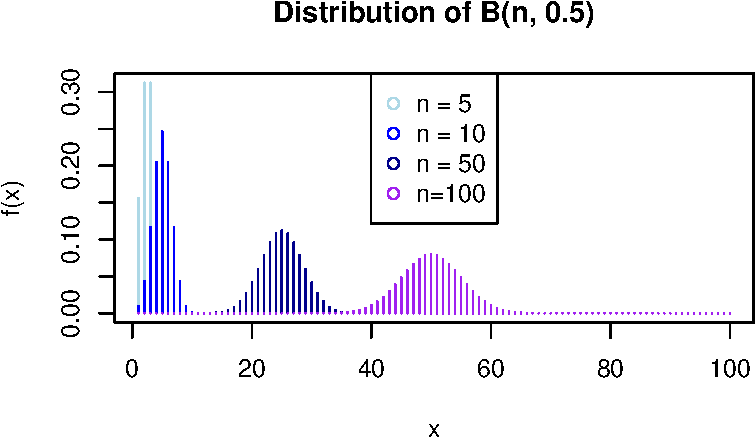
\includegraphics{054_distributions_discrete_files/figure-pdf/unnamed-chunk-6-1.pdf}

While we have looked at the distribution of the probabilities for a
total outcome after repetitions to be of a given ``exact'' value using
the density function \texttt{dbinom()}, we can use the cumulative form
\texttt{pbinom()} to know where the total outcome is smaller or equal to
a given value. For example, after 100 experiments with probability 0.5,
what is the probability I obtain less than 50 successes? Or \(n/2\)
successes depending on \(n\) ?

\begin{Shaded}
\begin{Highlighting}[]
\FunctionTok{pbinom}\NormalTok{(}\DecValTok{50}\NormalTok{, }\AttributeTok{size=}\DecValTok{100}\NormalTok{, }\AttributeTok{prob=}\FloatTok{0.5}\NormalTok{)}
\CommentTok{\#\textgreater{} [1] 0.5397946}
\FunctionTok{pbinom}\NormalTok{(}\DecValTok{5}\NormalTok{, }\AttributeTok{size=}\DecValTok{10}\NormalTok{, }\AttributeTok{prob=}\FloatTok{0.5}\NormalTok{)}
\CommentTok{\#\textgreater{} [1] 0.6230469}
\FunctionTok{pbinom}\NormalTok{(}\DecValTok{5000000}\NormalTok{, }\AttributeTok{size=}\DecValTok{10000000}\NormalTok{, }\AttributeTok{prob=}\FloatTok{0.5}\NormalTok{)}
\CommentTok{\#\textgreater{} [1] 0.5001262}
\end{Highlighting}
\end{Shaded}

The cumulative density function can be plotted as follows for different
probabilities and a given size:

\begin{Shaded}
\begin{Highlighting}[]
\FunctionTok{plot}\NormalTok{(}\FunctionTok{pbinom}\NormalTok{(}\DecValTok{1}\SpecialCharTok{:}\DecValTok{100}\NormalTok{,}\AttributeTok{size=}\DecValTok{100}\NormalTok{,}\AttributeTok{prob=}\FloatTok{0.10}\NormalTok{), }\AttributeTok{main =} \StringTok{\textquotesingle{}CDF of B(100, p)\textquotesingle{}}\NormalTok{, }\AttributeTok{ylab =} \StringTok{\textquotesingle{}f(x)\textquotesingle{}}\NormalTok{, }\AttributeTok{type=}\StringTok{"s"}\NormalTok{, }\AttributeTok{col =} \StringTok{\textquotesingle{}darkgreen\textquotesingle{}}\NormalTok{)}
\FunctionTok{lines}\NormalTok{(}\FunctionTok{pbinom}\NormalTok{(}\DecValTok{1}\SpecialCharTok{:}\DecValTok{100}\NormalTok{,}\AttributeTok{size=}\DecValTok{100}\NormalTok{,}\AttributeTok{prob=}\FloatTok{0.25}\NormalTok{), }\AttributeTok{type=}\StringTok{"s"}\NormalTok{, }\AttributeTok{col =} \StringTok{\textquotesingle{}lightgreen\textquotesingle{}}\NormalTok{)}
\FunctionTok{lines}\NormalTok{(}\FunctionTok{pbinom}\NormalTok{(}\DecValTok{1}\SpecialCharTok{:}\DecValTok{100}\NormalTok{,}\AttributeTok{size=}\DecValTok{100}\NormalTok{,}\AttributeTok{prob=}\FloatTok{0.5}\NormalTok{), }\AttributeTok{type=}\StringTok{"s"}\NormalTok{, }\AttributeTok{col =} \StringTok{\textquotesingle{}gold\textquotesingle{}}\NormalTok{)}
\FunctionTok{lines}\NormalTok{(}\FunctionTok{pbinom}\NormalTok{(}\DecValTok{1}\SpecialCharTok{:}\DecValTok{100}\NormalTok{,}\AttributeTok{size=}\DecValTok{100}\NormalTok{,}\AttributeTok{prob=}\FloatTok{0.75}\NormalTok{), }\AttributeTok{type=}\StringTok{"s"}\NormalTok{, }\AttributeTok{col =} \StringTok{\textquotesingle{}orange\textquotesingle{}}\NormalTok{)}
\FunctionTok{lines}\NormalTok{(}\FunctionTok{pbinom}\NormalTok{(}\DecValTok{1}\SpecialCharTok{:}\DecValTok{100}\NormalTok{,}\AttributeTok{size=}\DecValTok{100}\NormalTok{,}\AttributeTok{prob=}\FloatTok{0.9}\NormalTok{), }\AttributeTok{type=}\StringTok{"s"}\NormalTok{, }\AttributeTok{col =} \StringTok{\textquotesingle{}darkred\textquotesingle{}}\NormalTok{)}
\FunctionTok{legend}\NormalTok{(}\StringTok{"bottomright"}\NormalTok{,}\AttributeTok{pch=}\DecValTok{1}\NormalTok{,}
       \AttributeTok{legend =} \FunctionTok{c}\NormalTok{(}\StringTok{"p = 0.10"}\NormalTok{, }\StringTok{"p = 0.25"}\NormalTok{, }\StringTok{"p = 0.50"}\NormalTok{,}\StringTok{"p = 0.75"}\NormalTok{, }\StringTok{"p = 0.90"}\NormalTok{),}
       \AttributeTok{col =} \FunctionTok{c}\NormalTok{(}\StringTok{"darkgreen"}\NormalTok{,}\StringTok{"lightgreen"}\NormalTok{, }\StringTok{\textquotesingle{}gold\textquotesingle{}}\NormalTok{, }\StringTok{\textquotesingle{}orange\textquotesingle{}}\NormalTok{,}\StringTok{"darkred"}\NormalTok{))}
\end{Highlighting}
\end{Shaded}

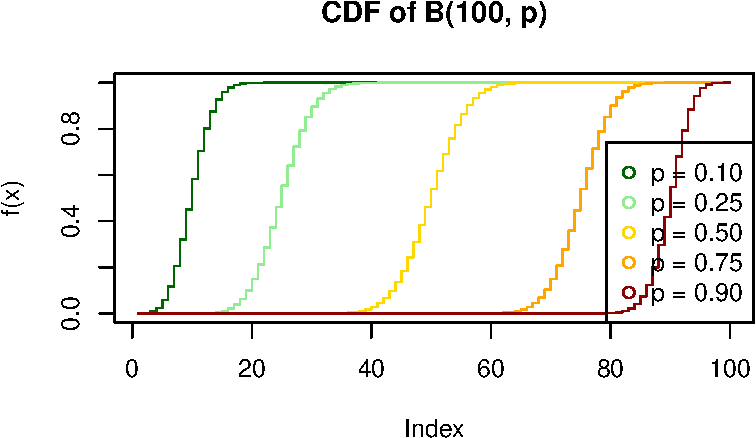
\includegraphics{054_distributions_discrete_files/figure-pdf/unnamed-chunk-8-1.pdf}

The binomial distribution is used in many cases where there are two
potential outcomes that are mutually exclusive. For example when we try
to explain why some plots of land are developed or not or why people use
the car rather than an active mode of transport.

\section{Discrete Poisson
distribution}\label{discrete-poisson-distribution}

The Poisson distribution is for rare discrete occurrence events. It is
used when counting the occurrence of a certain event that appears
randomly but at a known rate or density. The main statistical property
of the Poisson distribution is that \textbf{its variance equals its
mean}

There are many uses in geography, transport or planning, such as the
counting of cars passing a rural road segment over a certain time, or
the distribution of points (trees, bees, houses\ldots) over a
homogeneous set of spatial polygons (grid cells)

Suppose there are 100 houses or trees over 100 grid cells. The overall
density (\(\lambda\)) is 1. What is the probability that a cell does not
receive any single house? Or in other words what will be the proportion
of cells without a single house or tree?

\begin{Shaded}
\begin{Highlighting}[]
\FunctionTok{ppois}\NormalTok{(}\AttributeTok{lambda =} \DecValTok{1}\NormalTok{,}\AttributeTok{q=}\DecValTok{0}\NormalTok{)}
\CommentTok{\#\textgreater{} [1] 0.3678794}
\end{Highlighting}
\end{Shaded}

How does this change when the overall density is even higher or lower?
i.e.~with 150 houses/trees or only 25?

\begin{Shaded}
\begin{Highlighting}[]
\FunctionTok{ppois}\NormalTok{(}\AttributeTok{lambda =} \FloatTok{1.5}\NormalTok{,}\AttributeTok{q=}\DecValTok{0}\NormalTok{)}
\CommentTok{\#\textgreater{} [1] 0.2231302}
\FunctionTok{ppois}\NormalTok{(}\AttributeTok{lambda =} \FloatTok{0.5}\NormalTok{,}\AttributeTok{q=}\DecValTok{0}\NormalTok{)}
\CommentTok{\#\textgreater{} [1] 0.6065307}
\FunctionTok{ppois}\NormalTok{(}\AttributeTok{lambda =} \FloatTok{0.25}\NormalTok{,}\AttributeTok{q=}\DecValTok{0}\NormalTok{)}
\CommentTok{\#\textgreater{} [1] 0.7788008}
\end{Highlighting}
\end{Shaded}

Let's generate such cases and get the frequency of counts to ``see''
those occurrences:

\begin{Shaded}
\begin{Highlighting}[]
\NormalTok{pois025}\OtherTok{\textless{}{-}}\FunctionTok{rpois}\NormalTok{(}\DecValTok{100}\NormalTok{,}\FloatTok{0.25}\NormalTok{)}
\NormalTok{pois025}
\CommentTok{\#\textgreater{}   [1] 0 0 1 0 0 0 0 0 0 0 0 1 0 0 0 1 0 0 0 0 0 0 1 0 1 0 0 0 0 0 0 0 1 0 0 0 0}
\CommentTok{\#\textgreater{}  [38] 0 0 0 0 0 0 0 0 0 1 1 0 0 0 0 0 0 1 0 2 0 1 0 1 0 0 0 2 0 1 1 0 0 0 0 0 0}
\CommentTok{\#\textgreater{}  [75] 1 0 0 0 0 1 0 1 0 0 0 0 0 0 0 0 1 0 1 1 0 0 0 0 1 0}
\FunctionTok{table}\NormalTok{(pois025)}
\CommentTok{\#\textgreater{} pois025}
\CommentTok{\#\textgreater{}  0  1  2 }
\CommentTok{\#\textgreater{} 78 20  2}
\NormalTok{pois150}\OtherTok{\textless{}{-}}\FunctionTok{rpois}\NormalTok{(}\DecValTok{100}\NormalTok{,}\FloatTok{1.5}\NormalTok{)}
\NormalTok{pois150}
\CommentTok{\#\textgreater{}   [1] 1 1 0 5 1 0 3 0 0 2 2 5 0 1 3 0 2 1 2 4 2 0 1 0 1 1 1 1 1 3 1 1 0 1 3 1 4}
\CommentTok{\#\textgreater{}  [38] 1 0 1 3 3 2 1 1 1 1 0 3 3 0 0 0 0 1 2 0 0 0 1 3 5 1 1 4 1 1 1 0 3 1 2 1 2}
\CommentTok{\#\textgreater{}  [75] 3 1 0 1 2 1 3 4 1 5 0 3 1 2 1 1 4 3 1 1 3 1 0 1 3 2}
\FunctionTok{table}\NormalTok{(pois150)}
\CommentTok{\#\textgreater{} pois150}
\CommentTok{\#\textgreater{}  0  1  2  3  4  5 }
\CommentTok{\#\textgreater{} 22 41 12 16  5  4}
\end{Highlighting}
\end{Shaded}

We examine how the probability of different counts (not just 0 or more)
changes when lambda changes:

\begin{Shaded}
\begin{Highlighting}[]
\NormalTok{lambdan}\OtherTok{\textless{}{-}}\FunctionTok{data.frame}\NormalTok{(}\AttributeTok{n=}\FunctionTok{rep}\NormalTok{(}\DecValTok{1}\SpecialCharTok{:}\DecValTok{4}\NormalTok{,}\DecValTok{4}\NormalTok{),}\AttributeTok{lambda=}\FunctionTok{rep}\NormalTok{(}\FunctionTok{seq}\NormalTok{(}\DecValTok{1}\NormalTok{,}\FloatTok{0.25}\NormalTok{,}\AttributeTok{by=}\SpecialCharTok{{-}}\FloatTok{0.25}\NormalTok{),}\AttributeTok{each=}\DecValTok{4}\NormalTok{))}
\NormalTok{lambdan}\SpecialCharTok{$}\NormalTok{d}\OtherTok{\textless{}{-}}\FunctionTok{dpois}\NormalTok{(lambdan}\SpecialCharTok{$}\NormalTok{n,lambdan}\SpecialCharTok{$}\NormalTok{lambda)}
\NormalTok{lambdan}
\CommentTok{\#\textgreater{}    n lambda            d}
\CommentTok{\#\textgreater{} 1  1   1.00 0.3678794412}
\CommentTok{\#\textgreater{} 2  2   1.00 0.1839397206}
\CommentTok{\#\textgreater{} 3  3   1.00 0.0613132402}
\CommentTok{\#\textgreater{} 4  4   1.00 0.0153283100}
\CommentTok{\#\textgreater{} 5  1   0.75 0.3542749146}
\CommentTok{\#\textgreater{} 6  2   0.75 0.1328530930}
\CommentTok{\#\textgreater{} 7  3   0.75 0.0332132732}
\CommentTok{\#\textgreater{} 8  4   0.75 0.0062274887}
\CommentTok{\#\textgreater{} 9  1   0.50 0.3032653299}
\CommentTok{\#\textgreater{} 10 2   0.50 0.0758163325}
\CommentTok{\#\textgreater{} 11 3   0.50 0.0126360554}
\CommentTok{\#\textgreater{} 12 4   0.50 0.0015795069}
\CommentTok{\#\textgreater{} 13 1   0.25 0.1947001958}
\CommentTok{\#\textgreater{} 14 2   0.25 0.0243375245}
\CommentTok{\#\textgreater{} 15 3   0.25 0.0020281270}
\CommentTok{\#\textgreater{} 16 4   0.25 0.0001267579}
\end{Highlighting}
\end{Shaded}

Interesingly, the distribution depends on the segments of observations
or, in space, the rsolution of the grid, i.e.~the modifiable areal unit
problem (MAUP)

Consider the following:

Let's define a grid of 100 (10x10) cells over a mixed forest. Suppose a
poisson process with mean and variance = 1 gives the number of
coniferous trees within that forest. We can expect around 37 \% of cells
to have at least a coniferous, right? (see above).

Now suppose the mean and variance increase to 2, we are still in a
poisson process because the number of events is still quite rare even
there are less empty cells.

\begin{Shaded}
\begin{Highlighting}[]
\FunctionTok{ppois}\NormalTok{(}\AttributeTok{lambda=}\DecValTok{1}\NormalTok{, }\AttributeTok{q=}\DecValTok{0}\NormalTok{)}
\CommentTok{\#\textgreater{} [1] 0.3678794}
\FunctionTok{ppois}\NormalTok{(}\AttributeTok{lambda=}\DecValTok{2}\NormalTok{, }\AttributeTok{q=}\DecValTok{0}\NormalTok{)}
\CommentTok{\#\textgreater{} [1] 0.1353353}
\end{Highlighting}
\end{Shaded}

But if we now groups cells to make them larger, say divide the space
into 25 cells (5 x 5) rather than 100. Then you see that lambda is
multiplied by 4 and the probability of a zero count:

\begin{Shaded}
\begin{Highlighting}[]
\FunctionTok{ppois}\NormalTok{(}\AttributeTok{lambda=}\DecValTok{2}\SpecialCharTok{*}\DecValTok{4}\NormalTok{, }\AttributeTok{q=}\DecValTok{0}\NormalTok{)}
\CommentTok{\#\textgreater{} [1] 0.0003354626}
\end{Highlighting}
\end{Shaded}

Again, following the the Central Limit Theorem, the higher will be the
mean (λ) and thus the spatial aggregation, the closer the distribution
of coniferous will be to a normal distribution.

\begin{Shaded}
\begin{Highlighting}[]
\NormalTok{r2\_100}\OtherTok{\textless{}{-}}\FunctionTok{rpois}\NormalTok{(}\AttributeTok{lambda=}\DecValTok{2}\NormalTok{, }\AttributeTok{n=}\DecValTok{100}\NormalTok{)}
\NormalTok{r2\_100}
\CommentTok{\#\textgreater{}   [1] 0 0 2 0 3 1 0 1 4 4 3 4 2 0 4 1 0 3 1 3 3 0 5 3 2 1 1 3 0 0 5 2 2 1 4 3 1}
\CommentTok{\#\textgreater{}  [38] 1 4 2 3 0 0 2 1 2 0 1 2 2 1 5 4 3 4 0 3 1 3 1 1 3 3 3 2 2 2 2 5 1 2 2 2 5}
\CommentTok{\#\textgreater{}  [75] 4 7 2 3 3 1 1 3 1 1 2 1 1 3 1 0 0 1 1 1 3 1 4 4 2 2}
\FunctionTok{par}\NormalTok{(}\AttributeTok{mfrow =} \FunctionTok{c}\NormalTok{(}\DecValTok{1}\NormalTok{, }\DecValTok{2}\NormalTok{))}
\FunctionTok{image}\NormalTok{(}\FunctionTok{matrix}\NormalTok{(r2\_100, }\DecValTok{10}\NormalTok{),}\AttributeTok{asp=}\DecValTok{1}\NormalTok{)}
\FunctionTok{image}\NormalTok{(}\FunctionTok{matrix}\NormalTok{(r2\_100, }\DecValTok{10}\NormalTok{)}\SpecialCharTok{\textgreater{}}\DecValTok{1}\NormalTok{, }\AttributeTok{asp=}\DecValTok{1}\NormalTok{)}
\end{Highlighting}
\end{Shaded}

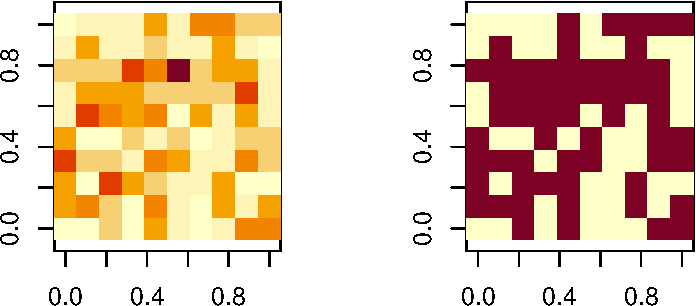
\includegraphics{054_distributions_discrete_files/figure-pdf/unnamed-chunk-15-1.pdf}

Re-aggregated:

\begin{Shaded}
\begin{Highlighting}[]
\NormalTok{large}\OtherTok{\textless{}{-}}\FunctionTok{matrix}\NormalTok{(}\FunctionTok{rep}\NormalTok{(}\DecValTok{1}\SpecialCharTok{:}\DecValTok{5}\NormalTok{,}\AttributeTok{each=}\DecValTok{20}\NormalTok{)}\SpecialCharTok{*}\DecValTok{10}\SpecialCharTok{+}\FunctionTok{rep}\NormalTok{(}\FunctionTok{rep}\NormalTok{(}\DecValTok{1}\SpecialCharTok{:}\DecValTok{5}\NormalTok{, }\AttributeTok{each=}\DecValTok{2}\NormalTok{),}\DecValTok{10}\NormalTok{),}\DecValTok{10}\NormalTok{)}
\NormalTok{large}
\CommentTok{\#\textgreater{}       [,1] [,2] [,3] [,4] [,5] [,6] [,7] [,8] [,9] [,10]}
\CommentTok{\#\textgreater{}  [1,]   11   11   21   21   31   31   41   41   51    51}
\CommentTok{\#\textgreater{}  [2,]   11   11   21   21   31   31   41   41   51    51}
\CommentTok{\#\textgreater{}  [3,]   12   12   22   22   32   32   42   42   52    52}
\CommentTok{\#\textgreater{}  [4,]   12   12   22   22   32   32   42   42   52    52}
\CommentTok{\#\textgreater{}  [5,]   13   13   23   23   33   33   43   43   53    53}
\CommentTok{\#\textgreater{}  [6,]   13   13   23   23   33   33   43   43   53    53}
\CommentTok{\#\textgreater{}  [7,]   14   14   24   24   34   34   44   44   54    54}
\CommentTok{\#\textgreater{}  [8,]   14   14   24   24   34   34   44   44   54    54}
\CommentTok{\#\textgreater{}  [9,]   15   15   25   25   35   35   45   45   55    55}
\CommentTok{\#\textgreater{} [10,]   15   15   25   25   35   35   45   45   55    55}

\NormalTok{sumbylarge}\OtherTok{\textless{}{-}}\FunctionTok{aggregate}\NormalTok{(r2\_100, }\AttributeTok{by=}\FunctionTok{list}\NormalTok{(}\FunctionTok{matrix}\NormalTok{(large)), }\AttributeTok{FUN=}\NormalTok{sum)}

\FunctionTok{matrix}\NormalTok{(sumbylarge}\SpecialCharTok{$}\NormalTok{x,}\DecValTok{5}\NormalTok{)}
\CommentTok{\#\textgreater{}      [,1] [,2] [,3] [,4] [,5]}
\CommentTok{\#\textgreater{} [1,]    7   10    9    8    5}
\CommentTok{\#\textgreater{} [2,]    4   11    9   13    4}
\CommentTok{\#\textgreater{} [3,]    9   10    7   15    7}
\CommentTok{\#\textgreater{} [4,]    4    6    5    9   12}
\CommentTok{\#\textgreater{} [5,]   12    6    8   10    5}

\FunctionTok{par}\NormalTok{(}\AttributeTok{mfrow =} \FunctionTok{c}\NormalTok{(}\DecValTok{1}\NormalTok{, }\DecValTok{2}\NormalTok{))}
\FunctionTok{image}\NormalTok{(}\FunctionTok{matrix}\NormalTok{(sumbylarge}\SpecialCharTok{$}\NormalTok{x,}\DecValTok{5}\NormalTok{))}
\FunctionTok{image}\NormalTok{(}\FunctionTok{matrix}\NormalTok{(sumbylarge}\SpecialCharTok{$}\NormalTok{x,}\DecValTok{5}\NormalTok{)}\SpecialCharTok{\textgreater{}}\DecValTok{1}\NormalTok{)}
\end{Highlighting}
\end{Shaded}

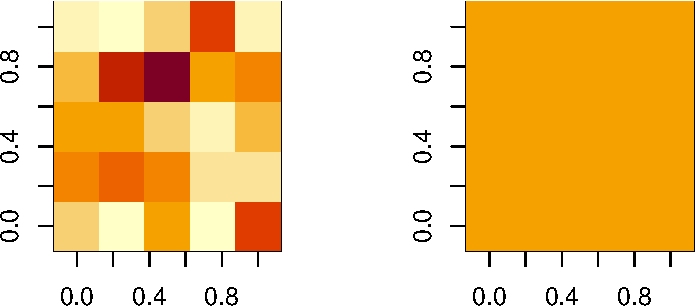
\includegraphics{054_distributions_discrete_files/figure-pdf/unnamed-chunk-16-1.pdf}

\part{Part VI - Statistical inference}

\chapter{Statistical Inference}\label{statistical-inference}

In this chapter, we first introduce point estimates and then confidence
interval estimations.

We will use a census extract of the US population as the main dataset,
\texttt{UScensus2000.txt} (see \texttt{data/US} folder)

\begin{Shaded}
\begin{Highlighting}[]
\NormalTok{census }\OtherTok{\textless{}{-}} \FunctionTok{read.table}\NormalTok{(}\StringTok{"data/US/UScensus2000.txt"}\NormalTok{, }
                     \AttributeTok{header =}\NormalTok{ T, }\AttributeTok{sep =} \StringTok{"}\SpecialCharTok{\textbackslash{}t}\StringTok{"}\NormalTok{)}
\FunctionTok{nrow}\NormalTok{(census)}
\CommentTok{\#\textgreater{} [1] 500}
\FunctionTok{summary}\NormalTok{(census)}
\CommentTok{\#\textgreater{}    censusYear   stateFIPScode      totalFamilyIncome      age      }
\CommentTok{\#\textgreater{}  Min.   :2000   Length:500         Min.   :     0    Min.   : 0.0  }
\CommentTok{\#\textgreater{}  1st Qu.:2000   Class :character   1st Qu.: 21500    1st Qu.:17.0  }
\CommentTok{\#\textgreater{}  Median :2000   Mode  :character   Median : 43000    Median :35.0  }
\CommentTok{\#\textgreater{}  Mean   :2000                      Mean   : 57411    Mean   :35.3  }
\CommentTok{\#\textgreater{}  3rd Qu.:2000                      3rd Qu.: 70700    3rd Qu.:51.0  }
\CommentTok{\#\textgreater{}  Max.   :2000                      Max.   :892050    Max.   :93.0  }
\CommentTok{\#\textgreater{}                                    NA\textquotesingle{}s   :15                      }
\CommentTok{\#\textgreater{}      sex            raceGeneral        maritalStatus      totalPersonalIncome}
\CommentTok{\#\textgreater{}  Length:500         Length:500         Length:500         Min.   : {-}4400     }
\CommentTok{\#\textgreater{}  Class :character   Class :character   Class :character   1st Qu.:  5900     }
\CommentTok{\#\textgreater{}  Mode  :character   Mode  :character   Mode  :character   Median : 17750     }
\CommentTok{\#\textgreater{}                                                           Mean   : 29082     }
\CommentTok{\#\textgreater{}                                                           3rd Qu.: 37000     }
\CommentTok{\#\textgreater{}                                                           Max.   :456000     }
\CommentTok{\#\textgreater{}                                                           NA\textquotesingle{}s   :108}
\end{Highlighting}
\end{Shaded}

\section{Point Estimates}\label{point-estimates}

To estimate the \emph{population mean} \(\bar{X}\) (or other metrics
such as variance or median) based on a sample, we typically use the
\emph{sample mean}:

\[\bar{x} = \dfrac{1}{n} \sum_{i=1}^n x_i\]

The sample mean, \(\bar{x}\), is known as a \textbf{point estimate} of
the \emph{population mean}.

\subsection{Problem}\label{problem}

If we draw another sample from the same population and calculate the new
sample mean, we are likely to obtain a different point estimate. This
difference is referred to as \textbf{sampling variation}.

In other words, an estimate is close to the true value but not exactly
equal to the actual (population) parameter value. Additionally, sampling
variation is expected to decrease as the sample size increases. A point
estimate converges to the population parameter value as the sample size
grows and approaches the size of the entire population.

\subsection{Example}\label{example}

We suppose that the dataset \texttt{census} contains our target
population. Our aim is to estimate the population mean for the variable
\texttt{age} and the proportion of the different genders in the case of
variable \texttt{sex}.

We look at the \emph{running mean} of the variable \texttt{age} and at
the \emph{running proportion} of men for the variable \texttt{sex}.

We start by extracting from the total population a sample made of one
observation: \(n = 1\). At each step, we extract randomly a new sample
with one additional observation. We use a sampling with replacement,
i.e.~the previous sample is not simply augmented: we take a new sample
(made of completely new individuals) each time. We stop when we reach
the total population, i.e.~when \(n = 500\) in our case.

The key function for sampling in R is \texttt{sample()}, which randomly
selects a number (arg \texttt{size}) of records for a given vector (or,
if none are specified, outputs a vector of \(1\) to \(size\) integers in
a random order, see below for examples of the \texttt{sample()}
function).

Note also that we introduce here a ``for loop'' to iterate from 1 to
\(N=500\) (our total population)

\begin{Shaded}
\begin{Highlighting}[]
\NormalTok{N }\OtherTok{\textless{}{-}} \FunctionTok{nrow}\NormalTok{(census) }\CommentTok{\#500}
\NormalTok{mu\_age }\OtherTok{\textless{}{-}} \FunctionTok{mean}\NormalTok{(census}\SpecialCharTok{$}\NormalTok{age) }\CommentTok{\#our population mean (usually unknown)}
\NormalTok{mu\_men }\OtherTok{\textless{}{-}} \FunctionTok{mean}\NormalTok{(census}\SpecialCharTok{$}\NormalTok{sex }\SpecialCharTok{==} \StringTok{\textquotesingle{}Male\textquotesingle{}}\NormalTok{) }\CommentTok{\#now our population proportion of males (usually unknown)}

\CommentTok{\#Prepare a vector of Means and Proportions}
\NormalTok{rMeanAge }\OtherTok{=} \ConstantTok{NULL}
\NormalTok{rPropMale }\OtherTok{=} \ConstantTok{NULL}

\FunctionTok{set.seed}\NormalTok{(}\DecValTok{201292}\NormalTok{)}

\ControlFlowTok{for}\NormalTok{ (i }\ControlFlowTok{in} \DecValTok{1}\SpecialCharTok{:}\NormalTok{N) \{}
\NormalTok{  sample }\OtherTok{\textless{}{-}}\NormalTok{ census[}\FunctionTok{sample}\NormalTok{(N, i), ]}
\NormalTok{  rMeanAge[i] }\OtherTok{\textless{}{-}} \FunctionTok{mean}\NormalTok{(sample}\SpecialCharTok{$}\NormalTok{age)}
\NormalTok{  rPropMale[i] }\OtherTok{\textless{}{-}} \FunctionTok{mean}\NormalTok{(sample}\SpecialCharTok{$}\NormalTok{sex }\SpecialCharTok{==} \StringTok{"Male"}\NormalTok{)}
\NormalTok{\}}
\FunctionTok{rm}\NormalTok{(sample) }\CommentTok{\#we don\textquotesingle{}t keep the last sample}

\FunctionTok{plot}\NormalTok{(rMeanAge, }\AttributeTok{type =} \StringTok{\textquotesingle{}l\textquotesingle{}}\NormalTok{, }\AttributeTok{col =} \DecValTok{2}\NormalTok{, }
     \AttributeTok{xlab =} \StringTok{\textquotesingle{}Sample size\textquotesingle{}}\NormalTok{, }\AttributeTok{ylab =} \StringTok{\textquotesingle{}age\textquotesingle{}}\NormalTok{, }
     \AttributeTok{main =} \StringTok{\textquotesingle{}Running mean\textquotesingle{}}\NormalTok{)}
\FunctionTok{abline}\NormalTok{(}\AttributeTok{h =}\NormalTok{ mu\_age, }\AttributeTok{col =} \StringTok{\textquotesingle{}darkgray\textquotesingle{}}\NormalTok{)}
\FunctionTok{text}\NormalTok{(}\DecValTok{500}\NormalTok{, mu\_age }\SpecialCharTok{+} \FloatTok{1.5}\NormalTok{, mu\_age, }\AttributeTok{col =} \StringTok{\textquotesingle{}darkgray\textquotesingle{}}\NormalTok{)}
\end{Highlighting}
\end{Shaded}

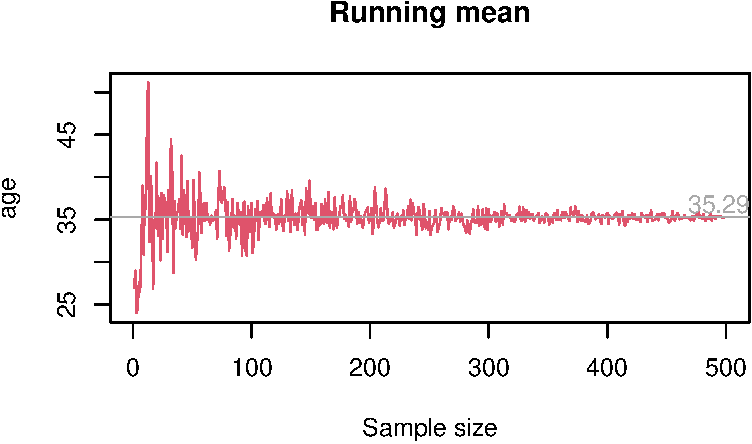
\includegraphics{061_inference_files/figure-pdf/runningMetrics-1.pdf}

\begin{Shaded}
\begin{Highlighting}[]

\FunctionTok{plot}\NormalTok{(rPropMale, }\AttributeTok{type =} \StringTok{\textquotesingle{}l\textquotesingle{}}\NormalTok{, }\AttributeTok{col =} \DecValTok{4}\NormalTok{, }
     \AttributeTok{xlab =} \StringTok{\textquotesingle{}Sample size\textquotesingle{}}\NormalTok{, }\AttributeTok{ylab =} \StringTok{\textquotesingle{}men\textquotesingle{}}\NormalTok{, }
     \AttributeTok{main =} \StringTok{\textquotesingle{}Running proportion\textquotesingle{}}\NormalTok{)}
\FunctionTok{abline}\NormalTok{(}\AttributeTok{h =}\NormalTok{ mu\_men, }\AttributeTok{col =} \StringTok{\textquotesingle{}darkgray\textquotesingle{}}\NormalTok{)}
\FunctionTok{text}\NormalTok{(}\DecValTok{500}\NormalTok{, mu\_men }\SpecialCharTok{+}\NormalTok{ .}\DecValTok{05}\NormalTok{, mu\_men, }\AttributeTok{col =} \StringTok{\textquotesingle{}darkgray\textquotesingle{}}\NormalTok{)}
\end{Highlighting}
\end{Shaded}

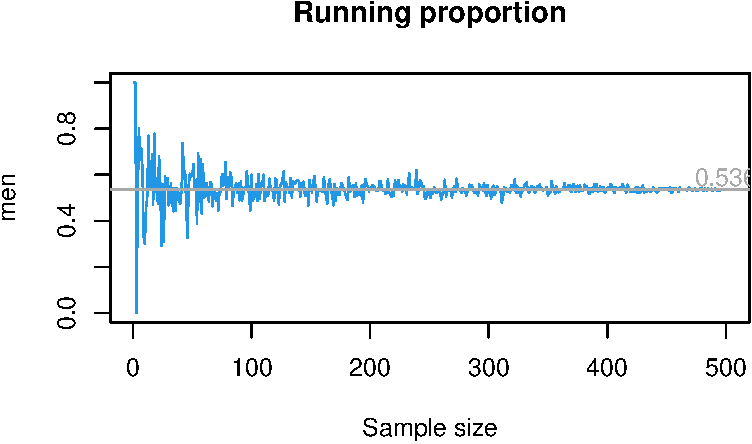
\includegraphics{061_inference_files/figure-pdf/runningMetrics-2.pdf}

\subsection{Standard Error}\label{standard-error}

To quantify the uncertainty of a point estimate, we use its
\textbf{standard error}. The standard error of an estimate (e.g.~the
mean) is the \textbf{standard deviation of its sampling distribution}.

The notion is not to be confused with the standard deviation of the
sample: - the \emph{standard error of the sample mean} indicates how far
the sample mean is from the population mean. - the \emph{standard
deviation of the sample} indicates how far each individual data within
the sample is from the sample mean.

The exact value of the standard error of the mean (or of the proportion)
is \[SE_{\bar{x}} = \dfrac{\sigma}{\sqrt{n}}\] which in our case can be
computed, given we know the population:

\begin{Shaded}
\begin{Highlighting}[]
\FunctionTok{sd}\NormalTok{(census}\SpecialCharTok{$}\NormalTok{age)}\SpecialCharTok{/}\FunctionTok{sqrt}\NormalTok{(N)}
\CommentTok{\#\textgreater{} [1] 0.9754678}
\FunctionTok{sd}\NormalTok{(census}\SpecialCharTok{$}\NormalTok{sex }\SpecialCharTok{==} \StringTok{"Male"}\NormalTok{)}\SpecialCharTok{/}\FunctionTok{sqrt}\NormalTok{(N)}
\CommentTok{\#\textgreater{} [1] 0.02232498}
\end{Highlighting}
\end{Shaded}

However, the standard deviation of the population is usually not known
and actually we would not need a point estimate and a standard error if
we were knowing the total population.

The standard error of the mean (or proportion) is thus estimated by
replacing \(\sigma\) in the definition with the standard deviation of
the sample used to make the point estimate, i.e.~\(s\)

\[SE_{\bar{x}} = \dfrac{s}{\sqrt{n}}\]

The denominator, \(\sqrt{n}\), reflects how the variability of the
sample mean decreases as the sample size increases. Also, due to the
square root, we see that a willingness to reduce the error of the
estimate by two requires four times as many observations.

Suppose a sample of 25 or 100 observations, the standard error would be

\begin{Shaded}
\begin{Highlighting}[]
\FunctionTok{set.seed}\NormalTok{(}\DecValTok{101}\NormalTok{)}
\NormalTok{sample\_age25 }\OtherTok{\textless{}{-}} \FunctionTok{sample}\NormalTok{(census}\SpecialCharTok{$}\NormalTok{age, }\DecValTok{25}\NormalTok{)}
\NormalTok{SEage25 }\OtherTok{\textless{}{-}} \FunctionTok{sd}\NormalTok{(sample\_age25) }\SpecialCharTok{/} \FunctionTok{sqrt}\NormalTok{(}\DecValTok{25}\NormalTok{)}
\NormalTok{SEage25}
\CommentTok{\#\textgreater{} [1] 4.464631}

\NormalTok{sample\_age100 }\OtherTok{\textless{}{-}} \FunctionTok{sample}\NormalTok{(census}\SpecialCharTok{$}\NormalTok{age, }\DecValTok{100}\NormalTok{)}
\NormalTok{SEage100 }\OtherTok{\textless{}{-}} \FunctionTok{sd}\NormalTok{(sample\_age100) }\SpecialCharTok{/} \FunctionTok{sqrt}\NormalTok{(}\DecValTok{100}\NormalTok{)}
\NormalTok{SEage100}
\CommentTok{\#\textgreater{} [1] 2.174494}

\NormalTok{sample\_sex25 }\OtherTok{\textless{}{-}} \FunctionTok{sample}\NormalTok{(census}\SpecialCharTok{$}\NormalTok{sex, }\DecValTok{25}\NormalTok{)}
\NormalTok{SEmen25 }\OtherTok{\textless{}{-}} \FunctionTok{sd}\NormalTok{(sample\_sex25 }\SpecialCharTok{==} \StringTok{\textquotesingle{}Male\textquotesingle{}}\NormalTok{) }\SpecialCharTok{/} \FunctionTok{sqrt}\NormalTok{(}\DecValTok{25}\NormalTok{)}
\NormalTok{SEmen25}
\CommentTok{\#\textgreater{} [1] 0.09797959}

\NormalTok{sample\_sex100 }\OtherTok{\textless{}{-}} \FunctionTok{sample}\NormalTok{(census}\SpecialCharTok{$}\NormalTok{sex, }\DecValTok{100}\NormalTok{)}
\NormalTok{SEmen100 }\OtherTok{\textless{}{-}} \FunctionTok{sd}\NormalTok{(sample\_sex100 }\SpecialCharTok{==} \StringTok{\textquotesingle{}Male\textquotesingle{}}\NormalTok{) }\SpecialCharTok{/} \FunctionTok{sqrt}\NormalTok{(}\DecValTok{100}\NormalTok{)}
\NormalTok{SEmen100}
\CommentTok{\#\textgreater{} [1] 0.04988877}
\end{Highlighting}
\end{Shaded}

where we see the reduction in error due to sample size. From 100 to 25,
the error is roughly halved The standard error of the mean of the sample
tends to zero when the sample size is increased. Indeed we have seen
earlier with the running means and proportions that sample means get
very close to the population mean when sample size is increased and
approaches the population.

\subsection{Sampling Distribution}\label{sampling-distribution}

Let's now build the \textbf{sampling distribution} of the sample mean.
So we can see the shape of that distribution and see that the standard
error is indeed the \textbf{standard deviation of the sampling
distribution}

We draw \(K = 1000\) samples of size \(n = 50\) from the population.

\begin{Shaded}
\begin{Highlighting}[]
\NormalTok{K }\OtherTok{\textless{}{-}} \DecValTok{1000}
\NormalTok{N}\OtherTok{\textless{}{-}}\FunctionTok{nrow}\NormalTok{(census)}
\NormalTok{n}\OtherTok{\textless{}{-}}\DecValTok{50}

\NormalTok{meanAge }\OtherTok{=} \ConstantTok{NULL}
\NormalTok{propMen }\OtherTok{=} \ConstantTok{NULL}

\FunctionTok{set.seed}\NormalTok{(}\DecValTok{345}\NormalTok{)}
\ControlFlowTok{for}\NormalTok{ (i }\ControlFlowTok{in} \DecValTok{1}\SpecialCharTok{:}\NormalTok{K) \{}
\NormalTok{  sample }\OtherTok{\textless{}{-}}\NormalTok{ census[}\FunctionTok{sample}\NormalTok{(N, n), ]}
\NormalTok{  meanAge[i] }\OtherTok{\textless{}{-}} \FunctionTok{mean}\NormalTok{(sample}\SpecialCharTok{$}\NormalTok{age)}
\NormalTok{  propMen[i] }\OtherTok{\textless{}{-}} \FunctionTok{mean}\NormalTok{(sample}\SpecialCharTok{$}\NormalTok{sex }\SpecialCharTok{==} \StringTok{\textquotesingle{}Male\textquotesingle{}}\NormalTok{)}
\NormalTok{\}}
\FunctionTok{rm}\NormalTok{(sample)}

\FunctionTok{hist}\NormalTok{(meanAge, }\AttributeTok{breaks =} \DecValTok{25}\NormalTok{,}
     \AttributeTok{main =} \StringTok{\textquotesingle{}Sampling distribution of the mean age\textquotesingle{}}\NormalTok{)}
\FunctionTok{abline}\NormalTok{(}\AttributeTok{v =}\NormalTok{ mu\_age, }\AttributeTok{col =} \DecValTok{2}\NormalTok{)}
\FunctionTok{text}\NormalTok{(}\FloatTok{38.5}\NormalTok{, }\DecValTok{100}\NormalTok{, mu\_age, }\AttributeTok{col =} \DecValTok{2}\NormalTok{)}
\end{Highlighting}
\end{Shaded}

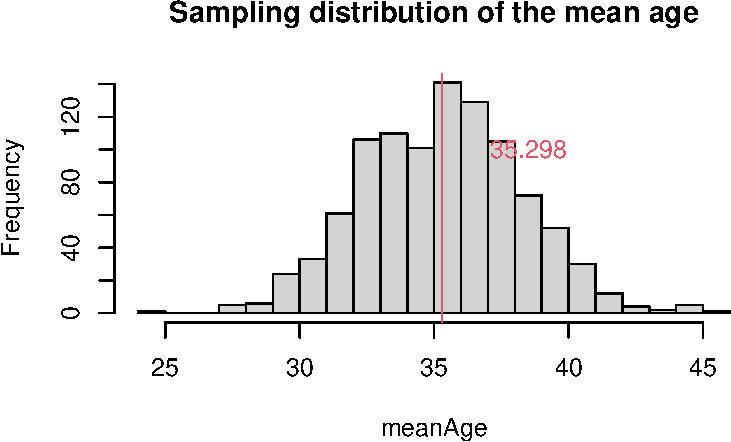
\includegraphics{061_inference_files/figure-pdf/unnamed-chunk-4-1.pdf}

\begin{Shaded}
\begin{Highlighting}[]

\FunctionTok{hist}\NormalTok{(propMen, }\AttributeTok{breaks =} \DecValTok{20}\NormalTok{,}
     \AttributeTok{main =} \StringTok{\textquotesingle{}Sampling distribution of the proportion of men\textquotesingle{}}\NormalTok{)}
\FunctionTok{abline}\NormalTok{(}\AttributeTok{v =}\NormalTok{ mu\_men, }\AttributeTok{col =} \DecValTok{2}\NormalTok{)}
\FunctionTok{text}\NormalTok{(mu\_men }\SpecialCharTok{+}\NormalTok{ .}\DecValTok{1}\NormalTok{, }\DecValTok{100}\NormalTok{, mu\_men, }\AttributeTok{col =} \DecValTok{2}\NormalTok{)}
\end{Highlighting}
\end{Shaded}

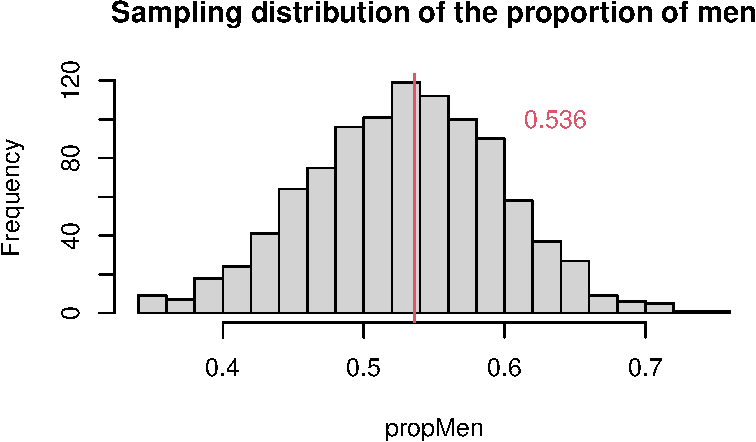
\includegraphics{061_inference_files/figure-pdf/unnamed-chunk-4-2.pdf}

In our case, the distribution of the mean and of the proportion are
symmetric and centered around the real value \(\mu = 35.298\)
(\texttt{mu\_age}) and \(\mu = 0.536\) (\texttt{mu\_men}).

Following the Central Limit Theorem, no matter whether the true
population is normal or not, the sample mean is approximately normally
distributed when sample size is large (we often see a value of \(> 30\)
to consider a sample is not small)

Since we are lucky enough to have a large amount of samples, we can
estimate the standard error directly form its definition, i.e.~the
standard deviation of the sample means.

In this case:

\begin{Shaded}
\begin{Highlighting}[]
\FunctionTok{sd}\NormalTok{(meanAge) }\CommentTok{\#standard deviation of the sample means}
\CommentTok{\#\textgreater{} [1] 2.970229}
\FunctionTok{sd}\NormalTok{(propMen) }\CommentTok{\#standard deviation of the sample proportions}
\CommentTok{\#\textgreater{} [1] 0.06858092}
\end{Highlighting}
\end{Shaded}

\section{Confidence Interval
Estimation}\label{confidence-interval-estimation}

Due to the error in point estimates, it is often relevant to look at
intervals instead of just the exact points. The range of values of
estimates for a given parameter is called a \textbf{confidence interval}
(CI). To build a confidence interval we need three elements:

\begin{itemize}
\tightlist
\item
  A point estimate \(\hat{\theta}\) for the parameter of interest
  \(\theta\)
\item
  The standard error associated with the point estimate
  \(SE_{\hat{\theta}}\)
\item
  A confidence level \(1 - \alpha\)
\end{itemize}

We know the first two elements. A confidence interval uses the
information about the uncertainty of the point estimate to define the
range of values such that we are confident at a level \(1 - \alpha\)
that it captures the true (population) parameter value. We call
\(1 - \alpha\) the \textbf{confidence level}.

For \(\alpha = 5\% = 0.05\), we can say that

\begin{quote}
\emph{``We are 95\% confident that the interval will capture the
population parameter.''}
\end{quote}

In other words:

\begin{quote}
\emph{``If we generate 100 samples, and compute their confidence
interval, in 95 cases, the interval will contain the parameter value''.}
\end{quote}

When a point estimate \(\hat{\theta}\) follows a normal distribution
(case of a sufficiently sample size), its confidence interval is defined
by: \[[\hat{\theta} \pm z_\alpha SE]\]

Here, \(z_\alpha SE\) is the \textbf{margin of error}.

Under a normal distribution:

\begin{itemize}
\tightlist
\item
  \(z_{0.1} = 1.645\): 90\% confidence interval
\item
  \(z_{0.05} = 1.96\): 95\% confidence interval
\item
  \(z_{0.001} = 2.58\): 99\% confidence interval
\end{itemize}

\subsection{Example}\label{example-1}

In the case of the age variable of the census data, the intervals for
each of our \(K\) samples are

\begin{Shaded}
\begin{Highlighting}[]
\NormalTok{CI95 }\OtherTok{\textless{}{-}} \FunctionTok{data.frame}\NormalTok{(}\AttributeTok{low =}\NormalTok{ meanAge }\SpecialCharTok{{-}} \FloatTok{1.96} \SpecialCharTok{*} \FunctionTok{sd}\NormalTok{(meanAge), }
                   \AttributeTok{point =}\NormalTok{ meanAge,}
                   \AttributeTok{high =}\NormalTok{ meanAge }\SpecialCharTok{+} \FloatTok{1.96} \SpecialCharTok{*} \FunctionTok{sd}\NormalTok{(meanAge))}

\FunctionTok{head}\NormalTok{(CI95)}
\CommentTok{\#\textgreater{}        low point     high}
\CommentTok{\#\textgreater{} 1 29.89835 35.72 41.54165}
\CommentTok{\#\textgreater{} 2 25.25835 31.08 36.90165}
\CommentTok{\#\textgreater{} 3 30.87835 36.70 42.52165}
\CommentTok{\#\textgreater{} 4 22.39835 28.22 34.04165}
\CommentTok{\#\textgreater{} 5 28.71835 34.54 40.36165}
\CommentTok{\#\textgreater{} 6 29.07835 34.90 40.72165}
\end{Highlighting}
\end{Shaded}

While in most cases, the interval is within the 95\% confidence range
around \(\mu = 35.298\), the upper bounds of the confidence intervals
for some of the samples can exceed
\(\mu + 1.96 \times SE_{\text{age}}\), indicating that these samples
have higher or lower sample means and greater variability, thus
suggesting they are less reliable as estimates of the population mean.

We can find out those cases for example as follow:

\begin{Shaded}
\begin{Highlighting}[]
\NormalTok{abov}\OtherTok{\textless{}{-}}\FunctionTok{which}\NormalTok{(CI95}\SpecialCharTok{$}\NormalTok{low}\SpecialCharTok{\textgreater{}}\NormalTok{mu\_age)}
\NormalTok{belo}\OtherTok{\textless{}{-}}\FunctionTok{which}\NormalTok{(CI95}\SpecialCharTok{$}\NormalTok{high}\SpecialCharTok{\textless{}}\NormalTok{mu\_age)}
\NormalTok{abov}
\CommentTok{\#\textgreater{}  [1]  57  68 172 175 190 209 244 277 477 505 548 571 606 631 692 748 786 810 839}
\CommentTok{\#\textgreater{} [20] 841 857 976 984}
\NormalTok{belo}
\CommentTok{\#\textgreater{}  [1]   4  12  81  93 137 139 148 187 197 261 380 400 432 461 633 644 763 773 853}
\CommentTok{\#\textgreater{} [20] 876 886}
\end{Highlighting}
\end{Shaded}

Interestingly, but not surprisingly, we can see there are roughly 25
cases where the CI range is too high and 25 where the CI range is too
low. Well that is 50 out 1000 samples and the exact meaning of
\(\alpha=0.05\):

\begin{quote}
\emph{If we generate 1000 samples, and compute their confidence
interval, in 950 cases, the interval will contain the parameter value.}
\end{quote}

We show the confidence interval for 3 samples (out of the 95\%) where
the point estimate can be trusted to represent the population mean,
followed by 3 of the too high cases and 3 of the too low cases.

\begin{Shaded}
\begin{Highlighting}[]
\NormalTok{a\_subset}\OtherTok{\textless{}{-}}\FunctionTok{c}\NormalTok{(}\DecValTok{1}\SpecialCharTok{:}\DecValTok{3}\NormalTok{,abov[}\DecValTok{1}\SpecialCharTok{:}\DecValTok{3}\NormalTok{],belo[}\DecValTok{1}\SpecialCharTok{:}\DecValTok{3}\NormalTok{])}
\FunctionTok{plot}\NormalTok{(CI95[a\_subset, }\StringTok{\textquotesingle{}low\textquotesingle{}}\NormalTok{], }\AttributeTok{col =} \StringTok{\textquotesingle{}darkgray\textquotesingle{}}\NormalTok{, }\AttributeTok{lwd =}\NormalTok{ .}\DecValTok{3}\NormalTok{, }
     \AttributeTok{type =} \StringTok{\textquotesingle{}b\textquotesingle{}}\NormalTok{, }\AttributeTok{ylim =} \FunctionTok{c}\NormalTok{(}\DecValTok{23}\NormalTok{,}\DecValTok{45}\NormalTok{), }
     \AttributeTok{xlab =} \StringTok{\textquotesingle{}sample\textquotesingle{}}\NormalTok{, }\AttributeTok{ylab =} \StringTok{\textquotesingle{}mean age\textquotesingle{}}\NormalTok{,}
     \AttributeTok{main =} \StringTok{\textquotesingle{}Confidence Intervals at level 95\%\textquotesingle{}}\NormalTok{,}
     \AttributeTok{xaxt=}\StringTok{"n"}\NormalTok{)}
\FunctionTok{lines}\NormalTok{(CI95[a\_subset, }\StringTok{\textquotesingle{}point\textquotesingle{}}\NormalTok{], }\AttributeTok{col =} \DecValTok{4}\NormalTok{, }\AttributeTok{type =} \StringTok{\textquotesingle{}b\textquotesingle{}}\NormalTok{)}
\FunctionTok{lines}\NormalTok{(CI95[a\_subset, }\StringTok{\textquotesingle{}high\textquotesingle{}}\NormalTok{], }\AttributeTok{col =} \StringTok{\textquotesingle{}darkgray\textquotesingle{}}\NormalTok{, }\AttributeTok{lwd =}\NormalTok{ .}\DecValTok{75}\NormalTok{, , }\AttributeTok{type =} \StringTok{\textquotesingle{}b\textquotesingle{}}\NormalTok{)}
\FunctionTok{abline}\NormalTok{(}\AttributeTok{h =}\NormalTok{ mu\_age, }\AttributeTok{col =} \DecValTok{2}\NormalTok{, }\AttributeTok{lwd =} \DecValTok{2}\NormalTok{)}
\FunctionTok{abline}\NormalTok{(}\AttributeTok{v =} \FloatTok{3.5}\NormalTok{, }\AttributeTok{lwd =} \FloatTok{0.5}\NormalTok{, }\AttributeTok{col=}\StringTok{"grey10"}\NormalTok{,}\AttributeTok{lty=}\DecValTok{2}\NormalTok{)}
\FunctionTok{abline}\NormalTok{(}\AttributeTok{v =} \FloatTok{6.5}\NormalTok{, }\AttributeTok{lwd =} \FloatTok{0.5}\NormalTok{, }\AttributeTok{col=}\StringTok{"grey10"}\NormalTok{,}\AttributeTok{lty=}\DecValTok{2}\NormalTok{)}
\FunctionTok{axis}\NormalTok{(}\DecValTok{1}\NormalTok{, }\AttributeTok{at=}\DecValTok{1}\SpecialCharTok{:}\FunctionTok{length}\NormalTok{(a\_subset), }\AttributeTok{labels=}\NormalTok{a\_subset,}\AttributeTok{las=}\DecValTok{2}\NormalTok{)}
\end{Highlighting}
\end{Shaded}

\begin{figure}[H]

{\centering 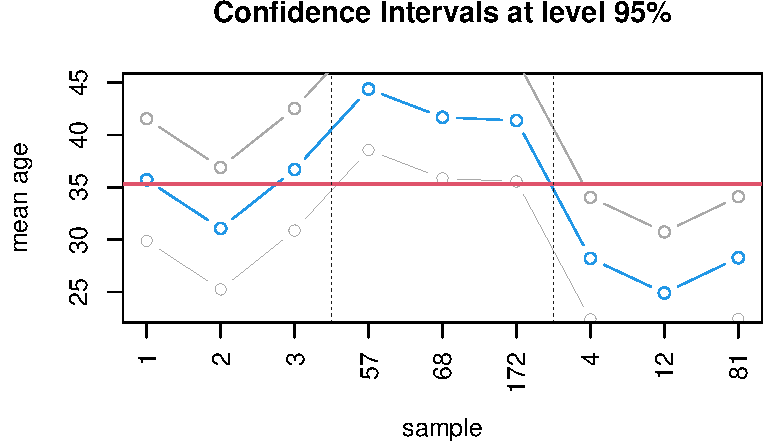
\includegraphics{061_inference_files/figure-pdf/unnamed-chunk-8-1.pdf}

}

\caption{Population mean in red = 35.298 ; some of the point estimates
in dark blue ; their corresponding confidence intervals at level 95\% in
gray}

\end{figure}%

Unfortunately, in the large majority of cases, we would not be able to
compute the standard error this way as we would only have one or two
samples. The only solution is then to use the standard deviation of the
sample divided by the square root of the sample size (see earlier
equations) as a best guess for the standard deviation of the
distribution of sample means, i.e.~to make up the standard error.

So far, we haven't stored that information (i.e.~standard deviation for
each sample). We need to relaunch the exact same samples (luckily we
used a seed). We do it for age only:

\begin{Shaded}
\begin{Highlighting}[]
\NormalTok{K }\OtherTok{\textless{}{-}} \DecValTok{1000}
\NormalTok{meanAge }\OtherTok{=} \ConstantTok{NULL}
\NormalTok{sdAge }\OtherTok{=} \ConstantTok{NULL}

\FunctionTok{set.seed}\NormalTok{(}\DecValTok{345}\NormalTok{)}
\ControlFlowTok{for}\NormalTok{ (i }\ControlFlowTok{in} \DecValTok{1}\SpecialCharTok{:}\NormalTok{K) \{}
\NormalTok{  sample }\OtherTok{\textless{}{-}}\NormalTok{ census[}\FunctionTok{sample}\NormalTok{(N, n), ]}
\NormalTok{  meanAge[i] }\OtherTok{\textless{}{-}} \FunctionTok{mean}\NormalTok{(sample}\SpecialCharTok{$}\NormalTok{age)}
\NormalTok{  sdAge[i] }\OtherTok{\textless{}{-}} \FunctionTok{sd}\NormalTok{(sample}\SpecialCharTok{$}\NormalTok{age)}
\NormalTok{\}}
\end{Highlighting}
\end{Shaded}

From each standard deviation, we compute the standard error:

\begin{Shaded}
\begin{Highlighting}[]
\NormalTok{seAge}\OtherTok{\textless{}{-}}\NormalTok{sdAge}\SpecialCharTok{/}\FunctionTok{sqrt}\NormalTok{(n) }\CommentTok{\#sample sd error }
\FunctionTok{head}\NormalTok{(seAge)}
\CommentTok{\#\textgreater{} [1] 3.112849 2.517504 3.298144 2.995001 3.229483 2.931775}
\FunctionTok{head}\NormalTok{(seAge}\SpecialCharTok{\textgreater{}}\FunctionTok{sd}\NormalTok{(meanAge)) }\CommentTok{\#compare sample standard error and sampling distribution st dev}
\CommentTok{\#\textgreater{} [1]  TRUE FALSE  TRUE  TRUE  TRUE FALSE}
\end{Highlighting}
\end{Shaded}

where we see there is variety which will also make the CI different (not
constant) for each sample and thus change the decision on the relevance
of each sample mean:

\begin{Shaded}
\begin{Highlighting}[]
\NormalTok{CI95s }\OtherTok{\textless{}{-}} \FunctionTok{data.frame}\NormalTok{(}\AttributeTok{low =}\NormalTok{ meanAge }\SpecialCharTok{{-}} \FloatTok{1.96} \SpecialCharTok{*}\NormalTok{ seAge, }
                   \AttributeTok{point =}\NormalTok{ meanAge,}
                   \AttributeTok{high =}\NormalTok{ meanAge }\SpecialCharTok{+} \FloatTok{1.96} \SpecialCharTok{*}\NormalTok{ seAge)}
\end{Highlighting}
\end{Shaded}

\begin{Shaded}
\begin{Highlighting}[]
\NormalTok{abovs}\OtherTok{\textless{}{-}}\FunctionTok{which}\NormalTok{(CI95s}\SpecialCharTok{$}\NormalTok{low}\SpecialCharTok{\textgreater{}}\NormalTok{mu\_age)}
\NormalTok{belos}\OtherTok{\textless{}{-}}\FunctionTok{which}\NormalTok{(CI95s}\SpecialCharTok{$}\NormalTok{high}\SpecialCharTok{\textless{}}\NormalTok{mu\_age)}
\NormalTok{abovs}
\CommentTok{\#\textgreater{}  [1]  57  68 172 175 190 209 277 477 505 548 571 606 748 786 792 810 813 839 857}
\CommentTok{\#\textgreater{} [20] 976}
\NormalTok{belos}
\CommentTok{\#\textgreater{}  [1]   4  12  80  81  93 117 137 139 148 187 197 261 278 380 400 432 461 471 633}
\CommentTok{\#\textgreater{} [20] 638 644 705 723 763 773 853 876 886}
\end{Highlighting}
\end{Shaded}

\begin{Shaded}
\begin{Highlighting}[]
\NormalTok{a\_subset}\OtherTok{\textless{}{-}}\FunctionTok{c}\NormalTok{(}\DecValTok{1}\SpecialCharTok{:}\DecValTok{3}\NormalTok{,abovs[}\DecValTok{1}\SpecialCharTok{:}\DecValTok{3}\NormalTok{],belos[}\DecValTok{1}\SpecialCharTok{:}\DecValTok{3}\NormalTok{])}
\FunctionTok{plot}\NormalTok{(CI95s[a\_subset, }\StringTok{\textquotesingle{}low\textquotesingle{}}\NormalTok{], }\AttributeTok{col =} \StringTok{\textquotesingle{}darkgray\textquotesingle{}}\NormalTok{, }\AttributeTok{lwd =}\NormalTok{ .}\DecValTok{3}\NormalTok{, }
     \AttributeTok{type =} \StringTok{\textquotesingle{}b\textquotesingle{}}\NormalTok{, }\AttributeTok{ylim =} \FunctionTok{c}\NormalTok{(}\DecValTok{23}\NormalTok{,}\DecValTok{45}\NormalTok{), }
     \AttributeTok{xlab =} \StringTok{\textquotesingle{}sample\textquotesingle{}}\NormalTok{, }\AttributeTok{ylab =} \StringTok{\textquotesingle{}mean age\textquotesingle{}}\NormalTok{,}
     \AttributeTok{main =} \StringTok{\textquotesingle{}Confidence Intervals at level 95\%\textquotesingle{}}\NormalTok{,}
     \AttributeTok{xaxt=}\StringTok{"n"}\NormalTok{)}
\FunctionTok{lines}\NormalTok{(CI95s[a\_subset, }\StringTok{\textquotesingle{}point\textquotesingle{}}\NormalTok{], }\AttributeTok{col =} \DecValTok{4}\NormalTok{, }\AttributeTok{type =} \StringTok{\textquotesingle{}b\textquotesingle{}}\NormalTok{)}
\FunctionTok{lines}\NormalTok{(CI95s[a\_subset, }\StringTok{\textquotesingle{}high\textquotesingle{}}\NormalTok{], }\AttributeTok{col =} \StringTok{\textquotesingle{}darkgray\textquotesingle{}}\NormalTok{, }\AttributeTok{lwd =}\NormalTok{ .}\DecValTok{75}\NormalTok{, , }\AttributeTok{type =} \StringTok{\textquotesingle{}b\textquotesingle{}}\NormalTok{)}
\FunctionTok{abline}\NormalTok{(}\AttributeTok{h =}\NormalTok{ mu\_age, }\AttributeTok{col =} \DecValTok{2}\NormalTok{, }\AttributeTok{lwd =} \DecValTok{2}\NormalTok{)}
\FunctionTok{abline}\NormalTok{(}\AttributeTok{v =} \FloatTok{3.5}\NormalTok{, }\AttributeTok{lwd =} \FloatTok{0.5}\NormalTok{, }\AttributeTok{col=}\StringTok{"grey10"}\NormalTok{,}\AttributeTok{lty=}\DecValTok{2}\NormalTok{)}
\FunctionTok{abline}\NormalTok{(}\AttributeTok{v =} \FloatTok{6.5}\NormalTok{, }\AttributeTok{lwd =} \FloatTok{0.5}\NormalTok{, }\AttributeTok{col=}\StringTok{"grey10"}\NormalTok{,}\AttributeTok{lty=}\DecValTok{2}\NormalTok{)}
\FunctionTok{axis}\NormalTok{(}\DecValTok{1}\NormalTok{, }\AttributeTok{at=}\DecValTok{1}\SpecialCharTok{:}\FunctionTok{length}\NormalTok{(a\_subset), }\AttributeTok{labels=}\NormalTok{a\_subset,}\AttributeTok{las=}\DecValTok{2}\NormalTok{)}
\end{Highlighting}
\end{Shaded}

\begin{figure}[H]

{\centering 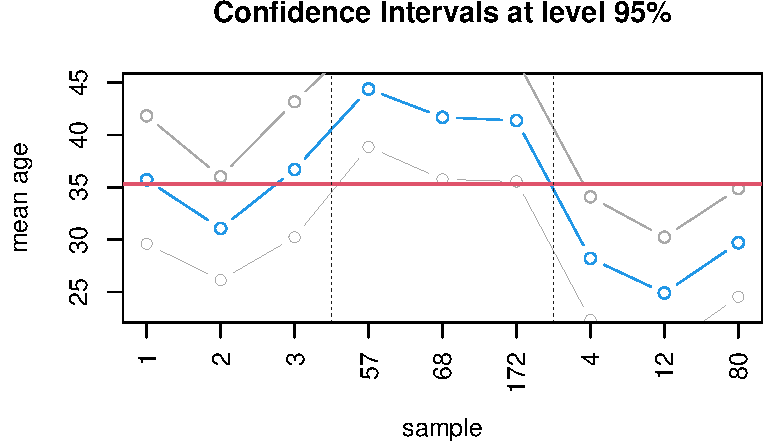
\includegraphics{061_inference_files/figure-pdf/unnamed-chunk-13-1.pdf}

}

\caption{Population mean in red = 35.298 ; some of the point estimates
in dark blue ; their corresponding confidence intervals at level 95\% in
gray}

\end{figure}%

The decision would have changed for some of the samples, for example 723
and 984, knowing \texttt{mu\_age} is 35.298.

\begin{Shaded}
\begin{Highlighting}[]
\FunctionTok{rbind}\NormalTok{(CI95s[}\FunctionTok{c}\NormalTok{(}\DecValTok{723}\NormalTok{),],CI95[}\FunctionTok{c}\NormalTok{(}\DecValTok{723}\NormalTok{),],CI95s[}\FunctionTok{c}\NormalTok{(}\DecValTok{984}\NormalTok{),],CI95[}\FunctionTok{c}\NormalTok{(}\DecValTok{984}\NormalTok{),])}
\CommentTok{\#\textgreater{}           low point     high}
\CommentTok{\#\textgreater{} 723  24.19980 29.72 35.24020}
\CommentTok{\#\textgreater{} 7231 23.89835 29.72 35.54165}
\CommentTok{\#\textgreater{} 984  35.09008 41.56 48.02992}
\CommentTok{\#\textgreater{} 9841 35.73835 41.56 47.38165}
\end{Highlighting}
\end{Shaded}

\subsection{\texorpdfstring{Note on the \texttt{sample()}
function}{Note on the sample() function}}\label{note-on-the-sample-function}

When applied to a vector x, \texttt{sample()} selects a set of values
within the vector. The size of this set (i.e.~the size of the sample) is
given though the argument \texttt{size}. Although there is no explicit
default to the argument (see help), it is inferred from the length of x
is not given. Hence when size is missing \texttt{sample(x)} provides a
random permutation of the vector x. Don't forget to use
\texttt{set.seed()} to keep a particular permutation

\begin{Shaded}
\begin{Highlighting}[]
\FunctionTok{set.seed}\NormalTok{(}\DecValTok{101}\NormalTok{)}
\FunctionTok{sample}\NormalTok{(}\FunctionTok{c}\NormalTok{(}\StringTok{"A"}\NormalTok{,}\StringTok{"B"}\NormalTok{,}\StringTok{"C"}\NormalTok{,}\StringTok{"D"}\NormalTok{))}
\CommentTok{\#\textgreater{} [1] "A" "D" "B" "C"}
\FunctionTok{set.seed}\NormalTok{(}\DecValTok{102}\NormalTok{)}
\FunctionTok{sample}\NormalTok{(}\FunctionTok{c}\NormalTok{(}\StringTok{"A"}\NormalTok{,}\StringTok{"B"}\NormalTok{,}\StringTok{"C"}\NormalTok{,}\StringTok{"D"}\NormalTok{))}
\CommentTok{\#\textgreater{} [1] "C" "B" "A" "D"}
\end{Highlighting}
\end{Shaded}

When size is explicit, a random subset is returned. In the case of a
random draw withour replacement (default) size cannot be smaller than
\texttt{length(x)}. It can if replacement is allowed:

\begin{Shaded}
\begin{Highlighting}[]
\FunctionTok{sample}\NormalTok{(}\FunctionTok{c}\NormalTok{(}\StringTok{"A"}\NormalTok{,}\StringTok{"B"}\NormalTok{,}\StringTok{"C"}\NormalTok{,}\StringTok{"D"}\NormalTok{),}\DecValTok{2}\NormalTok{)}
\CommentTok{\#\textgreater{} [1] "D" "C"}
\CommentTok{\#sample(c("A","B","C","D"),6) error}
\FunctionTok{sample}\NormalTok{(}\FunctionTok{c}\NormalTok{(}\StringTok{"A"}\NormalTok{,}\StringTok{"B"}\NormalTok{,}\StringTok{"C"}\NormalTok{,}\StringTok{"D"}\NormalTok{),}\DecValTok{10}\NormalTok{, }\AttributeTok{replace =} \ConstantTok{TRUE}\NormalTok{)}
\CommentTok{\#\textgreater{}  [1] "A" "D" "B" "D" "C" "C" "C" "A" "C" "C"}
\end{Highlighting}
\end{Shaded}

When applied to a scalar x, sample returns a random permutation of
values from 1 to x, or a subset of it if size is indicated:

\begin{Shaded}
\begin{Highlighting}[]
\FunctionTok{sample}\NormalTok{(}\DecValTok{7}\NormalTok{)}
\CommentTok{\#\textgreater{} [1] 6 5 4 7 1 2 3}
\FunctionTok{sample}\NormalTok{(}\DecValTok{7}\NormalTok{)}
\CommentTok{\#\textgreater{} [1] 6 2 7 3 4 1 5}
\FunctionTok{sample}\NormalTok{(}\DecValTok{7}\NormalTok{,}\AttributeTok{size=}\DecValTok{3}\NormalTok{)}
\CommentTok{\#\textgreater{} [1] 5 3 4}
\FunctionTok{sample}\NormalTok{(}\DecValTok{7}\NormalTok{,}\AttributeTok{size=}\DecValTok{10}\NormalTok{, }\AttributeTok{replace=}\ConstantTok{TRUE}\NormalTok{)}
\CommentTok{\#\textgreater{}  [1] 3 1 2 1 7 1 2 7 3 2}
\end{Highlighting}
\end{Shaded}

It is useful as such but also when applied to a data.frame.

For sampling a random set of rows over a data.frame you use sample with
a scalar corresponding to the number of rows in the data.frame. This
returns a random permutation of the identification of each row, which
you can then use to reshuffle or subset the data set:

\begin{Shaded}
\begin{Highlighting}[]
\NormalTok{data}\OtherTok{\textless{}{-}}\FunctionTok{data.frame}\NormalTok{(}\AttributeTok{Y=}\FunctionTok{c}\NormalTok{(}\StringTok{"A"}\NormalTok{,}\StringTok{"B"}\NormalTok{,}\StringTok{"C"}\NormalTok{,}\StringTok{"D"}\NormalTok{), }\AttributeTok{Z=}\DecValTok{11}\SpecialCharTok{:}\DecValTok{14}\NormalTok{)}
\NormalTok{data}
\CommentTok{\#\textgreater{}   Y  Z}
\CommentTok{\#\textgreater{} 1 A 11}
\CommentTok{\#\textgreater{} 2 B 12}
\CommentTok{\#\textgreater{} 3 C 13}
\CommentTok{\#\textgreater{} 4 D 14}

\FunctionTok{set.seed}\NormalTok{(}\DecValTok{101}\NormalTok{)}
\FunctionTok{sample}\NormalTok{(}\FunctionTok{nrow}\NormalTok{(data))}
\CommentTok{\#\textgreater{} [1] 1 4 2 3}

\CommentTok{\#reshuffle (permutation)}
\FunctionTok{set.seed}\NormalTok{(}\DecValTok{101}\NormalTok{)}
\NormalTok{data[}\FunctionTok{sample}\NormalTok{(}\FunctionTok{nrow}\NormalTok{(data)),]}
\CommentTok{\#\textgreater{}   Y  Z}
\CommentTok{\#\textgreater{} 1 A 11}
\CommentTok{\#\textgreater{} 4 D 14}
\CommentTok{\#\textgreater{} 2 B 12}
\CommentTok{\#\textgreater{} 3 C 13}

\CommentTok{\#random subset}
\FunctionTok{set.seed}\NormalTok{(}\DecValTok{101}\NormalTok{)}
\NormalTok{data[}\FunctionTok{sample}\NormalTok{(}\FunctionTok{nrow}\NormalTok{(data),}\AttributeTok{size=}\DecValTok{2}\NormalTok{),]}
\CommentTok{\#\textgreater{}   Y  Z}
\CommentTok{\#\textgreater{} 1 A 11}
\CommentTok{\#\textgreater{} 4 D 14}
\end{Highlighting}
\end{Shaded}

\subsection{Other example:}\label{other-example}

We have a sample of 100 trees with measurements of their diameter at
breast height. We are interested in the mean value and standard error.
The point estimate equals 164 with an empirical variance of 333221.

What is the standard error of the sample mean?

\begin{Shaded}
\begin{Highlighting}[]
\NormalTok{n }\OtherTok{\textless{}{-}} \DecValTok{100}
\NormalTok{variance }\OtherTok{\textless{}{-}} \DecValTok{333221}
\CommentTok{\# compute sample standard deviation}
\NormalTok{s }\OtherTok{\textless{}{-}} \FunctionTok{sqrt}\NormalTok{(variance)}
\NormalTok{s}
\CommentTok{\#\textgreater{} [1] 577.253}
\CommentTok{\# compute standard error of the sample mean}
\NormalTok{SE\_mean }\OtherTok{\textless{}{-}}\NormalTok{ s }\SpecialCharTok{/} \FunctionTok{sqrt}\NormalTok{(n)}
\NormalTok{SE\_mean}
\CommentTok{\#\textgreater{} [1] 57.7253}
\end{Highlighting}
\end{Shaded}

What is the standard error if the sample was made of 1000 trees?

\begin{Shaded}
\begin{Highlighting}[]
\NormalTok{SE\_mean }\OtherTok{\textless{}{-}}\NormalTok{ s }\SpecialCharTok{/} \FunctionTok{sqrt}\NormalTok{(}\DecValTok{1000}\NormalTok{)}
\NormalTok{SE\_mean}
\CommentTok{\#\textgreater{} [1] 18.25434}
\end{Highlighting}
\end{Shaded}

\chapter{Hypotheses testing}\label{hypotheses-testing}

In this section we will use again the dataset \texttt{UScensus2000.txt}

\begin{Shaded}
\begin{Highlighting}[]
\NormalTok{census }\OtherTok{\textless{}{-}} \FunctionTok{read.table}\NormalTok{(}\StringTok{"data/US/UScensus2000.txt"}\NormalTok{, }
                     \AttributeTok{header =}\NormalTok{ T, }\AttributeTok{sep =} \StringTok{"}\SpecialCharTok{\textbackslash{}t}\StringTok{"}\NormalTok{)}
\end{Highlighting}
\end{Shaded}

\section{Concepts and Definitions}\label{concepts-and-definitions}

\subsection{Test}\label{test}

A statistical test is a method used to determine whether there is a
significant difference between an expected model (or hypothesis) and the
observed data. It is used to assess whether observed differences are due
to random chance or if they are statistically significant, thereby
allowing to compare a hypothesis against the collected data.

You are interested in a particular question for which only two answers
are possible: \emph{yes} or \emph{no}. Each outcome is expressed as an
hypothesis: a \textbf{null hypothesis} \(H_0\) - it often represents the
hypothesis of no change - and an \textbf{alternative hypothesis} \(H_1\)
- it often represents the hypothesis of a change.

Your sample is made of observations assumed to be \emph{random} and
described by a \emph{statistical model}. The two possible answers to the
question of interest are:

\begin{itemize}
\item
  \emph{The null hypothesis is rejected}: it means that the answer to
  the question is \emph{yes}: the observed differences are significant
  and sufficiently large that they our hypothesis does not hold.
\item
  \emph{The null hypothesis is not rejected}: it means that the answer
  to the question is \emph{no}: the differences observed are due to
  randomness. With this data our hypothesis still holds.
\end{itemize}

\subsection{Example:}\label{example-2}

You want to answer the question: \emph{Does a given drug have an impact
on a particular disease?}

\begin{itemize}
\item
  The null hypothesis (\(H_0\)) is: \emph{The drug has no effect; the
  patient does not feel better or worse with the treatment.}
\item
  The alternative hypothesis (\(H_1\)) is: \emph{The drug has an effect
  (which can be either positive or negative).}
\end{itemize}

\subsection{Uni- and Bi-lateral Tests}\label{uni--and-bi-lateral-tests}

There are two types of tests: bilateral and unilateral.

\begin{itemize}
\item
  \textbf{Bilateral Test}: This test checks for any difference from the
  null hypothesis, whether it is higher or lower.
  \[H_0 = \{ \theta = \theta_0 \} \text{ and } H_1 = \{ \theta \neq \theta_0 \}\]
\item
  \textbf{Unilateral Test}: This test checks for a difference in a
  specific direction, either higher or lower.

  \begin{itemize}
  \tightlist
  \item
    \textbf{Right-tailed test}:
    \[H_0 = \{ \theta \leq \theta_0 \} \text{ and } H_1 = \{ \theta > \theta_0 \}\]
  \item
    \textbf{Left-tailed test}:
    \[H_0 = \{ \theta \geq \theta_0 \} \text{ and } H_1 = \{ \theta < \theta_0 \}\]
  \end{itemize}
\end{itemize}

\subsection{Types of Errors}\label{types-of-errors}

Decision error terms help us understand the likelihood of making
incorrect decisions. There are two types of errors:

\begin{longtable}[]{@{}lcc@{}}
\toprule\noalign{}
& \(H_0\) true & \(H_1\) true \\
\midrule\noalign{}
\endhead
\bottomrule\noalign{}
\endlastfoot
\(H_0\) not rejected & \(1 - \alpha\) & \(\beta\) \\
\(H_0\) rejected & \(\alpha\) & \(1 - \beta\) \\
\end{longtable}

In the table above, rows represent the decision made, while columns
represent the actual reality.

\begin{itemize}
\tightlist
\item
  \textbf{Type I Error} (\(\alpha\)):
\end{itemize}

This is the \textbf{significance level} of the test. It occurs when we
reject the null hypothesis (\(H_0\)) when it is actually true. This
error represents the probability of incorrectly concluding that there is
an effect when there is none. Common significance levels are 1\%, 5\%,
or 10\%.

\begin{itemize}
\tightlist
\item
  \textbf{Type II Error} (\(\beta\)):
\end{itemize}

This occurs when we fail to reject the null hypothesis (\(H_0\)) when
the alternative hypothesis (\(H_1\)) is actually true. This error
represents the probability of incorrectly concluding that there is no
effect when there is one.

\subsection{Power of a Test}\label{power-of-a-test}

The power of a test is given by \(1 - \beta\).

It represents the probability of correctly rejecting the null hypothesis
(\(H_0\)) when it is false. If the power of a test tends to 1 as the
sample size increases to infinity, the test is said to be
\textbf{consistent}.

\subsection{\texorpdfstring{Critical Region:
\(C_\alpha\)}{Critical Region: C\_\textbackslash alpha}}\label{critical-region-c_alpha}

To test if a point estimate \(\hat{\theta}\) is significantly different
from a null value \(\theta_0\), we must consider uncertainty. We use the
concept of the \textbf{confidence interval} (CI) introduced previously.
The confidence interval is also known as the \emph{acceptance region}.
Any value outside this interval falls into the \emph{rejection region},
which is called the \textbf{critical region} and can be expressed as:

\[CI_{1-\alpha} = [\theta_0 \pm z_\alpha * SE ] = [ \theta_0 - z_{\alpha/2} * SE ; \theta_0 + z_{1-\alpha/2} * SE ] \]

\[C_\alpha = [ min ; \theta_0 - z_{\alpha/2} * SE] \cup [ \theta_0 + z_{1-\alpha/2} * SE ; max ]\]{[}\^{}062\_hypothesis\_test-1{]}

From \(Z\) the value of the observed statistic we can decide to reject
or not the null hypothesis.

\begin{itemize}
\tightlist
\item
  If \(Z \in C_\alpha\), we reject \(H_0\)
\item
  If \(Z \notin C_\alpha\), we do not reject \(H_0\)
\end{itemize}

\subsection{P-Value:}\label{p-value}

Also called the \emph{probability value}, the p-value or \(p\)
corresponds to the probability that a given test statistic exceeds the
threshold value to fall within the rejection area when \(H_0\) is true.
It helps us determine the strength of the evidence against the null
hypothesis.

A low p-value (close to 0) indicates that the observed data is unlikely
under the null hypothesis, suggesting that we should reject \(H_0\).
Conversely, a high p-value suggests that the observed data is consistent
with \(H_0\), and we do not reject it.

\textbf{Decision Rule}: - If \(p.value < \alpha\), we reject \(H_0\). -
If \(p.value > \alpha\), we do not reject \(H_0\).

\section{Steps in practice}\label{steps-in-practice}

\begin{enumerate}
\def\labelenumi{\arabic{enumi}.}
\item
  Choose \(H_0\), \(H_1\), and \(\alpha\).
\item
  Define the test statistic.
\item
  \textbf{Using the Critical Region}
\end{enumerate}

\begin{itemize}
\tightlist
\item
  Compute the critical region \(C_\alpha\) with respect to \(\alpha\)
  and \(H_0\).
\item
  Compute the value of the test statistic from the observed sample.
\end{itemize}

or 3. \textbf{Using the P-Value}

\begin{itemize}
\tightlist
\item
  Compute the p-value from the sample.
\end{itemize}

\begin{enumerate}
\def\labelenumi{\arabic{enumi}.}
\setcounter{enumi}{3}
\tightlist
\item
  Conclusion: Reject or do not reject \(H_0\) at the significance level
  \(\alpha\).
\end{enumerate}

\section{Illustration}\label{illustration}

Suppose we have a parameter \(\theta\), observed twice: blue \(1.5\) and
green \(2.5\) Suppose the population is expected to follow a standard
normal distribution

\begin{Shaded}
\begin{Highlighting}[]
\FunctionTok{plot}\NormalTok{(x, y, }\AttributeTok{type=}\StringTok{\textquotesingle{}l\textquotesingle{}}\NormalTok{, }\AttributeTok{axes =}\NormalTok{ F, }\AttributeTok{xlab =} \StringTok{\textquotesingle{}\textquotesingle{}}\NormalTok{, }\AttributeTok{ylab =} \StringTok{\textquotesingle{}\textquotesingle{}}\NormalTok{,}
     \AttributeTok{main =} \StringTok{\textquotesingle{}\textquotesingle{}}\NormalTok{)}
\FunctionTok{axis}\NormalTok{(}\DecValTok{1}\NormalTok{, }\FunctionTok{mean}\NormalTok{(y), }\StringTok{\textquotesingle{}null}\SpecialCharTok{\textbackslash{}n}\StringTok{ value\textquotesingle{}}\NormalTok{, }\AttributeTok{col =} \StringTok{\textquotesingle{}red\textquotesingle{}}\NormalTok{, }\AttributeTok{col.axis =} \StringTok{\textquotesingle{}red\textquotesingle{}}\NormalTok{)}
\FunctionTok{axis}\NormalTok{(}\DecValTok{1}\NormalTok{, obs1, }\StringTok{\textquotesingle{}observed }\SpecialCharTok{\textbackslash{}n}\StringTok{ value\textquotesingle{}}\NormalTok{, }\AttributeTok{col =} \StringTok{\textquotesingle{}blue\textquotesingle{}}\NormalTok{, }\AttributeTok{col.axis =} \StringTok{\textquotesingle{}blue\textquotesingle{}}\NormalTok{)}
\FunctionTok{axis}\NormalTok{(}\DecValTok{1}\NormalTok{, obs2, }\StringTok{\textquotesingle{}observed}\SpecialCharTok{\textbackslash{}n}\StringTok{ value\textquotesingle{}}\NormalTok{, }\AttributeTok{col =} \StringTok{\textquotesingle{}green\textquotesingle{}}\NormalTok{, }\AttributeTok{col.axis =} \StringTok{\textquotesingle{}green\textquotesingle{}}\NormalTok{)}
\FunctionTok{text}\NormalTok{(}\SpecialCharTok{{-}}\DecValTok{3}\NormalTok{, .}\DecValTok{25}\NormalTok{, }\StringTok{"Distribution of the}\SpecialCharTok{\textbackslash{}n}\StringTok{ parameter if H0 true"}\NormalTok{)}
\end{Highlighting}
\end{Shaded}

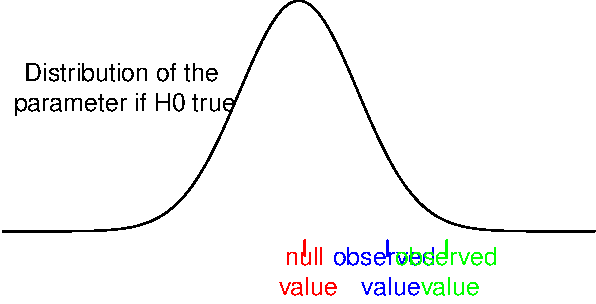
\includegraphics{062_hypotheses_test_files/figure-pdf/unnamed-chunk-3-1.pdf}

and we want to test the hypothesis \(H_0\) that those observed values
are not null, i.e.~testing the null hypothesis:
\(H_0: \theta = \theta_0\).

We choose a significance level \(\alpha = 5%
\)

The question is then: \emph{Are the observed value} \(\theta\)
significantly different from the null value \(\theta_0\) at level
\(\alpha = 5\%\)?

\textbf{Using the critical region} we observe the position of each
parameter against the values representing the limits of the critical
region:

We know the region is here defined based on a normal distribution of
mean 0 and standard deviation 1. So for \(\alpha = 5\%\), we have
\(z=-1.96\) and \(z=1.96\). Or more exactly

\begin{Shaded}
\begin{Highlighting}[]
\NormalTok{z }\OtherTok{\textless{}{-}} \FloatTok{1.96}
\FunctionTok{qnorm}\NormalTok{(}\AttributeTok{p=}\FloatTok{0.05}\SpecialCharTok{/}\DecValTok{2}\NormalTok{,}\AttributeTok{mean =} \DecValTok{0}\NormalTok{, }\AttributeTok{sd=}\DecValTok{1}\NormalTok{,}\AttributeTok{lower.tail =} \ConstantTok{TRUE}\NormalTok{)}
\CommentTok{\#\textgreater{} [1] {-}1.959964}
\FunctionTok{qnorm}\NormalTok{(}\AttributeTok{p=}\FloatTok{0.05}\SpecialCharTok{/}\DecValTok{2}\NormalTok{,}\AttributeTok{mean =} \DecValTok{0}\NormalTok{, }\AttributeTok{sd=}\DecValTok{1}\NormalTok{,}\AttributeTok{lower.tail =} \ConstantTok{FALSE}\NormalTok{)}
\CommentTok{\#\textgreater{} [1] 1.959964}
\end{Highlighting}
\end{Shaded}

\begin{Shaded}
\begin{Highlighting}[]
\FunctionTok{plot}\NormalTok{(x, y, }\AttributeTok{type=}\StringTok{\textquotesingle{}l\textquotesingle{}}\NormalTok{, }\AttributeTok{axes =}\NormalTok{ F, }\AttributeTok{xlab =} \StringTok{\textquotesingle{}\textquotesingle{}}\NormalTok{, }\AttributeTok{ylab =} \StringTok{\textquotesingle{}\textquotesingle{}}\NormalTok{,}
     \AttributeTok{main =} \StringTok{\textquotesingle{}alpha = 5\%}\SpecialCharTok{\textbackslash{}n}\StringTok{ Critical region\textquotesingle{}}\NormalTok{)}
\FunctionTok{axis}\NormalTok{(}\DecValTok{1}\NormalTok{, }\FunctionTok{mean}\NormalTok{(y), }\StringTok{\textquotesingle{}null}\SpecialCharTok{\textbackslash{}n}\StringTok{ value\textquotesingle{}}\NormalTok{, }\AttributeTok{col =} \StringTok{\textquotesingle{}red\textquotesingle{}}\NormalTok{, }\AttributeTok{col.axis =} \StringTok{\textquotesingle{}red\textquotesingle{}}\NormalTok{)}
\FunctionTok{axis}\NormalTok{(}\DecValTok{1}\NormalTok{, obs1, }\StringTok{\textquotesingle{}observed}\SpecialCharTok{\textbackslash{}n}\StringTok{ value\textquotesingle{}}\NormalTok{, }\AttributeTok{col =} \StringTok{\textquotesingle{}blue\textquotesingle{}}\NormalTok{, }\AttributeTok{col.axis =} \StringTok{\textquotesingle{}blue\textquotesingle{}}\NormalTok{)}
\FunctionTok{axis}\NormalTok{(}\DecValTok{1}\NormalTok{, obs2, }\StringTok{\textquotesingle{}observed}\SpecialCharTok{\textbackslash{}n}\StringTok{ value\textquotesingle{}}\NormalTok{, }\AttributeTok{col =} \StringTok{\textquotesingle{}green\textquotesingle{}}\NormalTok{, }\AttributeTok{col.axis =} \StringTok{\textquotesingle{}green\textquotesingle{}}\NormalTok{)}
\FunctionTok{text}\NormalTok{(}\SpecialCharTok{{-}}\DecValTok{3}\NormalTok{, .}\DecValTok{25}\NormalTok{, }\StringTok{"Distribution of the}\SpecialCharTok{\textbackslash{}n}\StringTok{ parameter if H0 true"}\NormalTok{)}

\FunctionTok{polygon}\NormalTok{(}\FunctionTok{c}\NormalTok{(z, x[x }\SpecialCharTok{\textgreater{}=}\NormalTok{ z]), }\FunctionTok{c}\NormalTok{(}\DecValTok{0}\NormalTok{, y[x }\SpecialCharTok{\textgreater{}=}\NormalTok{ z]), }\AttributeTok{col =} \StringTok{\textquotesingle{}purple\textquotesingle{}}\NormalTok{, }\AttributeTok{border =} \StringTok{\textquotesingle{}purple\textquotesingle{}}\NormalTok{)}
\FunctionTok{polygon}\NormalTok{(}\FunctionTok{c}\NormalTok{(}\SpecialCharTok{{-}}\NormalTok{z, x[x }\SpecialCharTok{\textless{}=} \SpecialCharTok{{-}}\NormalTok{z]), }\FunctionTok{c}\NormalTok{(}\DecValTok{0}\NormalTok{, y[x }\SpecialCharTok{\textless{}=} \SpecialCharTok{{-}}\NormalTok{z]), }\AttributeTok{col =} \StringTok{\textquotesingle{}purple\textquotesingle{}}\NormalTok{, }\AttributeTok{border =} \StringTok{\textquotesingle{}purple\textquotesingle{}}\NormalTok{)}
\FunctionTok{text}\NormalTok{(}\DecValTok{3}\NormalTok{, .}\DecValTok{08}\NormalTok{, }\StringTok{"P(X \textgreater{} 1.96) = 2.5\%}\SpecialCharTok{\textbackslash{}n}\StringTok{ = alpha/2"}\NormalTok{, }\AttributeTok{col =} \StringTok{\textquotesingle{}purple\textquotesingle{}}\NormalTok{)}
\FunctionTok{text}\NormalTok{(}\SpecialCharTok{{-}}\DecValTok{3}\NormalTok{, .}\DecValTok{08}\NormalTok{, }\StringTok{"P(X \textless{} {-}1.96) = 2.5\%}\SpecialCharTok{\textbackslash{}n}\StringTok{ = alpha/2"}\NormalTok{, }\AttributeTok{col =} \StringTok{\textquotesingle{}purple\textquotesingle{}}\NormalTok{)}
\end{Highlighting}
\end{Shaded}

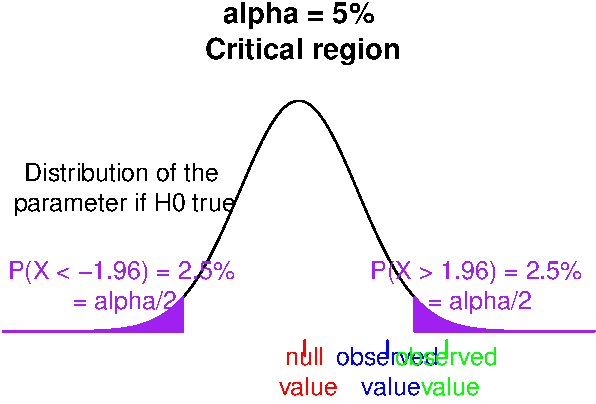
\includegraphics{062_hypotheses_test_files/figure-pdf/unnamed-chunk-5-1.pdf}

Now we see that:

\begin{itemize}
\tightlist
\item
  the green case is beyond the critical region for \(\theta\). We thus
  reject the null hypothesis. The green \(\theta\) is not zero.
\item
  the blue case is within the critical region for \(\theta\). We can't
  reject the null hypothesis. The blue \(\theta\) could still be a zero.
\end{itemize}

\textbf{Using the p-value}, we compute the corresponding p-values:

\begin{Shaded}
\begin{Highlighting}[]
\NormalTok{p1}\OtherTok{\textless{}{-}}\DecValTok{1}\SpecialCharTok{{-}}\FunctionTok{pnorm}\NormalTok{(}\AttributeTok{q =}\NormalTok{ obs1,}\AttributeTok{mean =} \DecValTok{0}\NormalTok{, }\AttributeTok{sd=}\DecValTok{1}\NormalTok{)}
\NormalTok{p1}
\CommentTok{\#\textgreater{} [1] 0.0668072}
\NormalTok{p2}\OtherTok{\textless{}{-}}\DecValTok{1}\SpecialCharTok{{-}}\FunctionTok{pnorm}\NormalTok{(}\AttributeTok{q =}\NormalTok{ obs2,}\AttributeTok{mean =} \DecValTok{0}\NormalTok{, }\AttributeTok{sd=}\DecValTok{1}\NormalTok{)}
\NormalTok{p2}
\CommentTok{\#\textgreater{} [1] 0.006209665}

\CommentTok{\#the p{-}value we chose can also be obtained from same function}
\NormalTok{qz}\OtherTok{\textless{}{-}}\FunctionTok{qnorm}\NormalTok{(}\AttributeTok{p =} \FloatTok{0.05}\SpecialCharTok{/}\DecValTok{2}\NormalTok{, }\AttributeTok{mean =} \DecValTok{0}\NormalTok{, }\AttributeTok{sd =} \DecValTok{1}\NormalTok{, }\AttributeTok{lower.tail =} \ConstantTok{FALSE}\NormalTok{)}
\NormalTok{qz}
\CommentTok{\#\textgreater{} [1] 1.959964}
\NormalTok{pz}\OtherTok{\textless{}{-}}\DecValTok{1}\SpecialCharTok{{-}}\FunctionTok{pnorm}\NormalTok{(}\AttributeTok{q=}\NormalTok{qz , }\AttributeTok{mean =} \DecValTok{0}\NormalTok{, }\AttributeTok{sd =} \DecValTok{1}\NormalTok{)}
\NormalTok{pz}
\CommentTok{\#\textgreater{} [1] 0.025}
\end{Highlighting}
\end{Shaded}

Where we see that - \(p.value = 0.06  > \alpha\) for the blue case,
i.e.~we reject \(H_0\). - \(p.value = 0.006  < \alpha\) for the green
case, i.e.~we don't reject \(H_0\).

\begin{Shaded}
\begin{Highlighting}[]
\FunctionTok{plot}\NormalTok{(x, y, }\AttributeTok{type=}\StringTok{\textquotesingle{}l\textquotesingle{}}\NormalTok{, }\AttributeTok{axes =}\NormalTok{ F, }\AttributeTok{xlab =} \StringTok{\textquotesingle{}\textquotesingle{}}\NormalTok{, }\AttributeTok{ylab =} \StringTok{\textquotesingle{}\textquotesingle{}}\NormalTok{,}
     \AttributeTok{main =} \StringTok{\textquotesingle{}alpha = 5\%}\SpecialCharTok{\textbackslash{}n}\StringTok{ P{-}value\textquotesingle{}}\NormalTok{)}
\FunctionTok{polygon}\NormalTok{(}\FunctionTok{c}\NormalTok{(obs1, x[x }\SpecialCharTok{\textgreater{}=}\NormalTok{ obs1]), }\FunctionTok{c}\NormalTok{(}\DecValTok{0}\NormalTok{, y[x }\SpecialCharTok{\textgreater{}=}\NormalTok{ obs1]), }\AttributeTok{col =} \StringTok{\textquotesingle{}blue\textquotesingle{}}\NormalTok{, }\AttributeTok{border =} \StringTok{\textquotesingle{}blue\textquotesingle{}}\NormalTok{)}
\FunctionTok{text}\NormalTok{(obs1}\SpecialCharTok{+}\DecValTok{1}\NormalTok{, .}\DecValTok{09}\NormalTok{, }\StringTok{"p.value"}\NormalTok{, }\AttributeTok{col =} \StringTok{\textquotesingle{}blue\textquotesingle{}}\NormalTok{)}
\FunctionTok{polygon}\NormalTok{(}\FunctionTok{c}\NormalTok{(z, x[x }\SpecialCharTok{\textgreater{}=}\NormalTok{ z]), }\FunctionTok{c}\NormalTok{(}\DecValTok{0}\NormalTok{, y[x }\SpecialCharTok{\textgreater{}=}\NormalTok{ z]), }\AttributeTok{col =} \StringTok{\textquotesingle{}purple\textquotesingle{}}\NormalTok{, }\AttributeTok{border =} \StringTok{\textquotesingle{}purple\textquotesingle{}}\NormalTok{)}
\FunctionTok{text}\NormalTok{(z}\FloatTok{+.5}\NormalTok{, .}\DecValTok{06}\NormalTok{, }\StringTok{"alpha"}\NormalTok{, }\AttributeTok{col =} \StringTok{\textquotesingle{}purple\textquotesingle{}}\NormalTok{)}
\FunctionTok{polygon}\NormalTok{(}\FunctionTok{c}\NormalTok{(obs2, x[x }\SpecialCharTok{\textgreater{}=}\NormalTok{ obs2]), }\FunctionTok{c}\NormalTok{(}\DecValTok{0}\NormalTok{, y[x }\SpecialCharTok{\textgreater{}=}\NormalTok{ obs2]), }\AttributeTok{col =} \StringTok{\textquotesingle{}green\textquotesingle{}}\NormalTok{, }\AttributeTok{border =} \StringTok{\textquotesingle{}green\textquotesingle{}}\NormalTok{)}
\FunctionTok{text}\NormalTok{(obs2}\SpecialCharTok{+}\DecValTok{1}\NormalTok{, .}\DecValTok{09}\NormalTok{, }\StringTok{"p.value"}\NormalTok{, }\AttributeTok{col =} \StringTok{\textquotesingle{}green\textquotesingle{}}\NormalTok{)}
\end{Highlighting}
\end{Shaded}

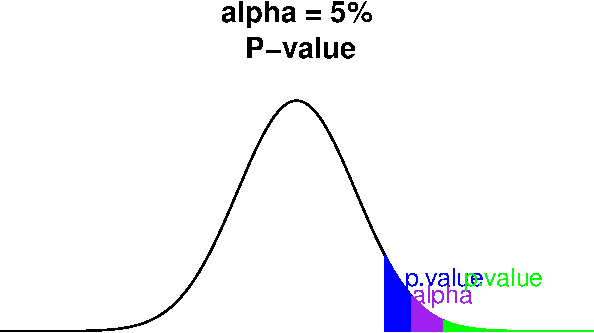
\includegraphics{062_hypotheses_test_files/figure-pdf/unnamed-chunk-7-1.pdf}

\section{Example: Testing the Average
Height}\label{example-testing-the-average-height}

Suppose we have a sample of 30 individuals, and we want to test if their
average height is significantly different from the known population mean
height of 170 cm.

Here is our sample (on purpose we generate it with an expected mean of
172 and quite a large variance)

\begin{Shaded}
\begin{Highlighting}[]
\FunctionTok{set.seed}\NormalTok{(}\DecValTok{123}\NormalTok{)}
\NormalTok{h }\OtherTok{\textless{}{-}} \FunctionTok{rnorm}\NormalTok{(}\DecValTok{30}\NormalTok{, }\AttributeTok{mean =} \DecValTok{172}\NormalTok{, }\AttributeTok{sd =} \DecValTok{6}\NormalTok{)}
\FunctionTok{summary}\NormalTok{(h)}
\CommentTok{\#\textgreater{}    Min. 1st Qu.  Median    Mean 3rd Qu.    Max. }
\CommentTok{\#\textgreater{}   160.2   168.0   171.6   171.7   174.9   182.7}
\FunctionTok{mean}\NormalTok{(h)}
\CommentTok{\#\textgreater{} [1] 171.7174}
\end{Highlighting}
\end{Shaded}

We know the population mean and consider a significance level of
\(0.05\)

\begin{Shaded}
\begin{Highlighting}[]
\NormalTok{barH }\OtherTok{\textless{}{-}} \DecValTok{170}
\NormalTok{alpha }\OtherTok{\textless{}{-}} \FloatTok{0.05}
\end{Highlighting}
\end{Shaded}

We would like to know if the sample mean is close to the population
mean, but we have a small number of records and the variance of the
population is not know, so we can't relate to a known normal
distribution but must consider a t-student distribution.

Our t-statistic compares the sample mean to the population mean divided
by the standard error:

\begin{Shaded}
\begin{Highlighting}[]
\NormalTok{t\_statistic }\OtherTok{\textless{}{-}}\NormalTok{ (}\FunctionTok{mean}\NormalTok{(h) }\SpecialCharTok{{-}}\NormalTok{ barH) }\SpecialCharTok{/}\NormalTok{ (}\FunctionTok{sd}\NormalTok{(h) }\SpecialCharTok{/} \FunctionTok{sqrt}\NormalTok{(}\FunctionTok{length}\NormalTok{(h)))}
\NormalTok{t\_statistic}
\CommentTok{\#\textgreater{} [1] 1.598058}
\end{Highlighting}
\end{Shaded}

We must compare this t-statistic to the value from a two-tailed t-test
critical value (our mean could be below or above the mean) with 29
degrees of freedom:

\begin{Shaded}
\begin{Highlighting}[]
\NormalTok{df }\OtherTok{\textless{}{-}} \FunctionTok{length}\NormalTok{(h) }\SpecialCharTok{{-}} \DecValTok{1}
\NormalTok{t\_critical }\OtherTok{\textless{}{-}} \FunctionTok{qt}\NormalTok{(}\DecValTok{1} \SpecialCharTok{{-}}\NormalTok{ alpha }\SpecialCharTok{/} \DecValTok{2}\NormalTok{, df)}
\NormalTok{t\_critical}
\CommentTok{\#\textgreater{} [1] 2.04523}
\end{Highlighting}
\end{Shaded}

Using the critical region, we can check if the parameter is beyond the
limits or not:

\begin{Shaded}
\begin{Highlighting}[]
\FunctionTok{abs}\NormalTok{(t\_statistic) }\SpecialCharTok{\textgreater{}}\NormalTok{ t\_critical}
\CommentTok{\#\textgreater{} [1] FALSE}
\end{Highlighting}
\end{Shaded}

, which in this case is \texttt{false} hence the sample mean is within
the acceptable range to correspond to the population mean. We can't
reject the null hypothesis.

We can also compute the p-value:

\begin{Shaded}
\begin{Highlighting}[]
\NormalTok{p\_value }\OtherTok{\textless{}{-}} \DecValTok{2} \SpecialCharTok{*}\NormalTok{ (}\DecValTok{1} \SpecialCharTok{{-}} \FunctionTok{pt}\NormalTok{(}\FunctionTok{abs}\NormalTok{(t\_statistic), df))}
\NormalTok{p\_value}
\CommentTok{\#\textgreater{} [1] 0.1208704}
\end{Highlighting}
\end{Shaded}

, which is above \(\alpha\). Hence we can't reject the null hypothesis.
The sample mean is not different form the population mean.

\chapter{Hypotheses testing - One sample
tests}\label{hypotheses-testing---one-sample-tests}

\section{Tests about a Mean}\label{tests-about-a-mean}

\subsection{Mean of normal distribution with known variance
(Z-Test)}\label{mean-of-normal-distribution-with-known-variance-z-test}

We consider a random variable \(X \sim N(\mu, \sigma^2)\) with \(\mu\)
unknown but \(\sigma^2\) being known - \emph{a very unrealistic case in
practice}. We use a sample of size \(n\): \(x = {x_1, x_2,..., x_n}\)
made of independent realizations of that random variable \(X\).

\begin{itemize}
\tightlist
\item
  \textbf{Testing}: \(H_0: \mu = \mu_0\) against
  \(H_1: \mu \neq \mu_0\).
\item
  \textbf{Test Statistic}: random variable defined by
  \[Z_n = \dfrac{\hat{\mu_n} - \mu_0}{\sigma / \sqrt{n}} \sim N(0, 1)\]
\item
  \textbf{The critical values} are read on a standard normal
  distribution table.
\end{itemize}

\subsubsection{Example (using summary description of
sample):}\label{example-using-summary-description-of-sample}

Suppose a population with the following characteristics:

\begin{Shaded}
\begin{Highlighting}[]
\NormalTok{mu\_0 }\OtherTok{\textless{}{-}} \DecValTok{50} \CommentTok{\#hypothesized population mean against which the test is made}
\NormalTok{sigma }\OtherTok{\textless{}{-}} \DecValTok{10} \CommentTok{\#population sd}
\end{Highlighting}
\end{Shaded}

And a sample of 25 records with a mean of 55

\begin{Shaded}
\begin{Highlighting}[]
\NormalTok{n }\OtherTok{\textless{}{-}} \DecValTok{25} \CommentTok{\#sample size}
\NormalTok{sample\_mean }\OtherTok{\textless{}{-}} \DecValTok{55}
\end{Highlighting}
\end{Shaded}

The test statistic is

\begin{Shaded}
\begin{Highlighting}[]
\NormalTok{Z\_n }\OtherTok{\textless{}{-}}\NormalTok{ (sample\_mean }\SpecialCharTok{{-}}\NormalTok{ mu\_0) }\SpecialCharTok{/}\NormalTok{ (sigma }\SpecialCharTok{/} \FunctionTok{sqrt}\NormalTok{(n))}
\NormalTok{Z\_n}
\CommentTok{\#\textgreater{} [1] 2.5}
\end{Highlighting}
\end{Shaded}

With a given significance level, you then decide to reject or not the
null hypothesis (equal means)

\begin{Shaded}
\begin{Highlighting}[]
\NormalTok{alpha }\OtherTok{\textless{}{-}} \FloatTok{0.05}
\CommentTok{\# Determine the critical value and decide:}
\NormalTok{Z\_alpha }\OtherTok{\textless{}{-}} \FunctionTok{qnorm}\NormalTok{(}\DecValTok{1} \SpecialCharTok{{-}}\NormalTok{ alpha }\SpecialCharTok{/} \DecValTok{2}\NormalTok{)}
\NormalTok{Z\_alpha}
\CommentTok{\#\textgreater{} [1] 1.959964}
\NormalTok{reject\_H0 }\OtherTok{\textless{}{-}} \FunctionTok{abs}\NormalTok{(Z\_n) }\SpecialCharTok{\textgreater{}}\NormalTok{ Z\_alpha}
\NormalTok{reject\_H0}
\CommentTok{\#\textgreater{} [1] TRUE}

\CommentTok{\# or Calculate the p{-}value and decide:}
\NormalTok{p\_value }\OtherTok{\textless{}{-}} \DecValTok{2} \SpecialCharTok{*}\NormalTok{ (}\DecValTok{1} \SpecialCharTok{{-}} \FunctionTok{pnorm}\NormalTok{(}\FunctionTok{abs}\NormalTok{(Z\_n)))}
\NormalTok{p\_value}
\CommentTok{\#\textgreater{} [1] 0.01241933}
\NormalTok{reject\_H0 }\OtherTok{\textless{}{-}}\NormalTok{ p\_value }\SpecialCharTok{\textless{}}\NormalTok{ alpha}
\NormalTok{reject\_H0}
\CommentTok{\#\textgreater{} [1] TRUE}
\end{Highlighting}
\end{Shaded}

Suppose another example with sample mean closer to the hypothesized
population mean, then

\begin{Shaded}
\begin{Highlighting}[]
\NormalTok{sample\_mean }\OtherTok{\textless{}{-}} \DecValTok{51}
\NormalTok{Z\_n }\OtherTok{\textless{}{-}}\NormalTok{ (sample\_mean }\SpecialCharTok{{-}}\NormalTok{ mu\_0) }\SpecialCharTok{/}\NormalTok{ (sigma }\SpecialCharTok{/} \FunctionTok{sqrt}\NormalTok{(n))}
\NormalTok{p\_value }\OtherTok{\textless{}{-}} \DecValTok{2} \SpecialCharTok{*}\NormalTok{ (}\DecValTok{1} \SpecialCharTok{{-}} \FunctionTok{pnorm}\NormalTok{(}\FunctionTok{abs}\NormalTok{(Z\_n)))}
\NormalTok{p\_value}
\CommentTok{\#\textgreater{} [1] 0.6170751}
\NormalTok{reject\_H0 }\OtherTok{\textless{}{-}}\NormalTok{ p\_value }\SpecialCharTok{\textless{}}\NormalTok{ alpha}
\NormalTok{reject\_H0}
\CommentTok{\#\textgreater{} [1] FALSE}
\end{Highlighting}
\end{Shaded}

\subsection{Mean of normal distribution with unknown variance
(t-test)}\label{mean-of-normal-distribution-with-unknown-variance-t-test}

In reality, it is far more likely you don't know the population
variance.

We consider a random variable \(X \sim N(\mu, \sigma^2)\) with \(\mu\)
and \(\sigma^2\) unknown. We use a sample of size \(n\):
\(x = {x_1, x_2,..., x_n}\) made of independent realizations of that
random variable \(X\).

\begin{itemize}
\tightlist
\item
  \textbf{Testing}: \(H_0: \mu = \mu_0\) against
  \(H_1: \mu \neq \mu_0\).
\item
  \textbf{Test Statistic}: random variable defined by
  \[T_{n-1} = \dfrac{\hat{\mu_n} - \mu_0}{S_{n,c} / \sqrt{n}} \sim t(n-1)\]
\item
  \textbf{Decision rule}: the critical value \(c_\alpha\) is read on a
  student distribution table.
\item
  \textbf{The critical values} are read on a t-student distribution
  table, which we know doesn't need a variance to be defined.
\end{itemize}

\subsubsection{Example (using a summary description of a
sample)}\label{example-using-a-summary-description-of-a-sample}

Suppose the same example as for the Z-test but this time we don't know
the population variance. We can't use \(\sigma\) but can still compute
the sample variance (or standard deviation)

\begin{Shaded}
\begin{Highlighting}[]
\NormalTok{sample\_mean }\OtherTok{\textless{}{-}} \DecValTok{55}
\NormalTok{sample\_sd }\OtherTok{\textless{}{-}} \DecValTok{10}
\end{Highlighting}
\end{Shaded}

and then the t-test:

\begin{Shaded}
\begin{Highlighting}[]
\NormalTok{T\_n }\OtherTok{\textless{}{-}}\NormalTok{ (sample\_mean }\SpecialCharTok{{-}}\NormalTok{ mu\_0) }\SpecialCharTok{/}\NormalTok{ (sample\_sd }\SpecialCharTok{/} \FunctionTok{sqrt}\NormalTok{(n))}
\NormalTok{T\_n}
\CommentTok{\#\textgreater{} [1] 2.5}
\end{Highlighting}
\end{Shaded}

So we can now decide (using the p-value)

\begin{Shaded}
\begin{Highlighting}[]
\NormalTok{p\_value }\OtherTok{\textless{}{-}} \DecValTok{2} \SpecialCharTok{*}\NormalTok{ (}\DecValTok{1} \SpecialCharTok{{-}} \FunctionTok{pt}\NormalTok{(}\FunctionTok{abs}\NormalTok{(T\_n), }\AttributeTok{df =}\NormalTok{ n }\SpecialCharTok{{-}} \DecValTok{1}\NormalTok{))}
\NormalTok{p\_value}
\CommentTok{\#\textgreater{} [1] 0.01965418}
\NormalTok{reject\_H0 }\OtherTok{\textless{}{-}}\NormalTok{ p\_value }\SpecialCharTok{\textless{}}\NormalTok{ alpha}
\NormalTok{reject\_H0}
\CommentTok{\#\textgreater{} [1] TRUE}
\end{Highlighting}
\end{Shaded}

Again, if the sample mean was closer to the population one, for this
same observed variance, we would have:

\begin{Shaded}
\begin{Highlighting}[]
\NormalTok{sample\_mean }\OtherTok{\textless{}{-}} \DecValTok{51}
\NormalTok{T\_n }\OtherTok{\textless{}{-}}\NormalTok{ (sample\_mean }\SpecialCharTok{{-}}\NormalTok{ mu\_0) }\SpecialCharTok{/}\NormalTok{ (sample\_sd }\SpecialCharTok{/} \FunctionTok{sqrt}\NormalTok{(n))}
\NormalTok{p\_value }\OtherTok{\textless{}{-}} \DecValTok{2} \SpecialCharTok{*}\NormalTok{ (}\DecValTok{1} \SpecialCharTok{{-}} \FunctionTok{pt}\NormalTok{(}\FunctionTok{abs}\NormalTok{(T\_n), }\AttributeTok{df =}\NormalTok{ n }\SpecialCharTok{{-}} \DecValTok{1}\NormalTok{))}
\NormalTok{p\_value}
\CommentTok{\#\textgreater{} [1] 0.6216287}
\NormalTok{reject\_H0 }\OtherTok{\textless{}{-}}\NormalTok{ p\_value }\SpecialCharTok{\textless{}}\NormalTok{ alpha}
\NormalTok{reject\_H0}
\CommentTok{\#\textgreater{} [1] FALSE}
\end{Highlighting}
\end{Shaded}

\subsubsection{Example (using the sample data
itself)}\label{example-using-the-sample-data-itself}

Suppose we have the actual sample data instead of just the summary
statistics. We can perform the t-test using the \texttt{t.test()}
function in R (still using the hypothesized mean of 50), with the
advantage of not having to compute the sample mean and staandard
deviation and a reporting of bot p-value and confidence interval

\begin{Shaded}
\begin{Highlighting}[]
\NormalTok{sample\_data }\OtherTok{\textless{}{-}} \FunctionTok{c}\NormalTok{(}\DecValTok{55}\NormalTok{, }\DecValTok{51}\NormalTok{, }\DecValTok{49}\NormalTok{, }\DecValTok{52}\NormalTok{, }\DecValTok{56}\NormalTok{, }\DecValTok{54}\NormalTok{, }\DecValTok{50}\NormalTok{, }\DecValTok{53}\NormalTok{, }\DecValTok{57}\NormalTok{, }\DecValTok{58}\NormalTok{)}
\FunctionTok{t.test}\NormalTok{(sample\_data, }\AttributeTok{mu =}\NormalTok{ mu\_0)}
\CommentTok{\#\textgreater{} }
\CommentTok{\#\textgreater{}  One Sample t{-}test}
\CommentTok{\#\textgreater{} }
\CommentTok{\#\textgreater{} data:  sample\_data}
\CommentTok{\#\textgreater{} t = 3.6556, df = 9, p{-}value = 0.005271}
\CommentTok{\#\textgreater{} alternative hypothesis: true mean is not equal to 50}
\CommentTok{\#\textgreater{} 95 percent confidence interval:}
\CommentTok{\#\textgreater{}  51.33415 55.66585}
\CommentTok{\#\textgreater{} sample estimates:}
\CommentTok{\#\textgreater{} mean of x }
\CommentTok{\#\textgreater{}      53.5}
\end{Highlighting}
\end{Shaded}

which holds the same result as our earlier ``manual'' method using the
summary statistics of the sample, see:

\begin{Shaded}
\begin{Highlighting}[]
\NormalTok{n}\OtherTok{\textless{}{-}}\FunctionTok{length}\NormalTok{(sample\_data)}
\NormalTok{sample\_mean}\OtherTok{\textless{}{-}}\FunctionTok{mean}\NormalTok{(sample\_data)}
\NormalTok{sample\_sd}\OtherTok{\textless{}{-}}\FunctionTok{sd}\NormalTok{(sample\_data)}
\NormalTok{p\_value }\OtherTok{\textless{}{-}} \DecValTok{2} \SpecialCharTok{*}\NormalTok{ (}\DecValTok{1} \SpecialCharTok{{-}} \FunctionTok{pt}\NormalTok{(}\FunctionTok{abs}\NormalTok{((sample\_mean }\SpecialCharTok{{-}}\NormalTok{ mu\_0) }\SpecialCharTok{/}\NormalTok{ (sample\_sd }\SpecialCharTok{/} \FunctionTok{sqrt}\NormalTok{(n))), }\AttributeTok{df =}\NormalTok{ n }\SpecialCharTok{{-}} \DecValTok{1}\NormalTok{))}
\NormalTok{p\_value}
\CommentTok{\#\textgreater{} [1] 0.005271186}
\end{Highlighting}
\end{Shaded}

\section{Tests about a Variance}\label{tests-about-a-variance}

\subsection{Variance of normal distribution with known mean (chi-squared
test n
df)}\label{variance-of-normal-distribution-with-known-mean-chi-squared-test-n-df}

We consider a random variable \(X \sim N(\mu, \sigma^2)\) with \(\mu\)
known and \(\sigma^2\) unknown - \emph{quite rare in practice}. We use a
sample of size \(n\): \(x = {x_1, x_2,..., x_n}\) made of independent
realizations of that random variable \(X\).

\begin{itemize}
\tightlist
\item
  \textbf{Testing}: \(H_0: \sigma^2 = \sigma^2_0\) against
  \(H_1: \sigma^2 \neq \sigma^2_0\).
\item
  \textbf{Test Statistic}: random variable defined by
  \[\chi^2_{n} = \dfrac{(n) \hat{\sigma^2_n}}{\sigma^2} \sim \chi^2(n)\]
\item
  \textbf{The critical values} are read on a chi-squared distribution
  table. After a sampling from a normal distribution, the distribution
  of the sample variance is known to follow a chi-squared distribution.
\end{itemize}

\subsubsection{Example:}\label{example-3}

Considering the same hypothetical population and a generated normal
sample of 30 observations (for which the true standard deviation is
higher, i.e.~15).

\begin{Shaded}
\begin{Highlighting}[]
\FunctionTok{set.seed}\NormalTok{(}\DecValTok{123}\NormalTok{)}
\NormalTok{n}\OtherTok{\textless{}{-}}\DecValTok{30}
\NormalTok{x }\OtherTok{\textless{}{-}} \FunctionTok{rnorm}\NormalTok{(n, }\AttributeTok{mean =} \DecValTok{50}\NormalTok{, }\AttributeTok{sd =} \DecValTok{15}\NormalTok{)}
\NormalTok{sample\_variance }\OtherTok{\textless{}{-}} \FunctionTok{var}\NormalTok{(x)}
\FunctionTok{sd}\NormalTok{(x)}
\CommentTok{\#\textgreater{} [1] 14.71546}
\end{Highlighting}
\end{Shaded}

\begin{Shaded}
\begin{Highlighting}[]
\NormalTok{sigma\_0}\OtherTok{\textless{}{-}}\DecValTok{10}
\NormalTok{chi\_squared\_stat }\OtherTok{\textless{}{-}}\NormalTok{ (n }\SpecialCharTok{*}\NormalTok{ sample\_variance) }\SpecialCharTok{/}\NormalTok{ sigma\_0}\SpecialCharTok{\^{}}\DecValTok{2}
\NormalTok{chi\_squared\_stat}
\CommentTok{\#\textgreater{} [1] 64.96343}
\end{Highlighting}
\end{Shaded}

\begin{Shaded}
\begin{Highlighting}[]
\NormalTok{alpha}\OtherTok{\textless{}{-}}\FloatTok{0.05}
\NormalTok{critical\_value\_lower }\OtherTok{\textless{}{-}} \FunctionTok{qchisq}\NormalTok{(alpha }\SpecialCharTok{/} \DecValTok{2}\NormalTok{, }\AttributeTok{df =}\NormalTok{ n)}
\NormalTok{critical\_value\_upper }\OtherTok{\textless{}{-}} \FunctionTok{qchisq}\NormalTok{(}\DecValTok{1} \SpecialCharTok{{-}}\NormalTok{ alpha }\SpecialCharTok{/} \DecValTok{2}\NormalTok{, }\AttributeTok{df =}\NormalTok{ n)}
\FunctionTok{c}\NormalTok{(critical\_value\_lower,critical\_value\_upper)}
\CommentTok{\#\textgreater{} [1] 16.79077 46.97924}

\CommentTok{\#or p{-}value}
\FunctionTok{pchisq}\NormalTok{(chi\_squared\_stat, }\AttributeTok{df =}\NormalTok{ n)}
\CommentTok{\#\textgreater{} [1] 0.9997783}
\NormalTok{p\_value }\OtherTok{\textless{}{-}} \DecValTok{2} \SpecialCharTok{*} \FunctionTok{min}\NormalTok{(}\FunctionTok{pchisq}\NormalTok{(chi\_squared\_stat, }\AttributeTok{df =}\NormalTok{ n), }\DecValTok{1} \SpecialCharTok{{-}} \FunctionTok{pchisq}\NormalTok{(chi\_squared\_stat, }\AttributeTok{df =}\NormalTok{ n))}
\NormalTok{p\_value}
\CommentTok{\#\textgreater{} [1] 0.0004434497}

\NormalTok{reject\_H0 }\OtherTok{\textless{}{-}}\NormalTok{ p\_value }\SpecialCharTok{\textless{}}\NormalTok{ alpha}
\NormalTok{reject\_H0}
\CommentTok{\#\textgreater{} [1] TRUE}
\end{Highlighting}
\end{Shaded}

Suppose another sample (generated with its true standard deviation, the
same as the population's)

\begin{Shaded}
\begin{Highlighting}[]
\FunctionTok{set.seed}\NormalTok{(}\DecValTok{101112}\NormalTok{)}
\NormalTok{n}\OtherTok{\textless{}{-}}\DecValTok{30}
\NormalTok{x }\OtherTok{\textless{}{-}} \FunctionTok{rnorm}\NormalTok{(n, }\AttributeTok{mean =} \DecValTok{50}\NormalTok{, }\AttributeTok{sd =} \DecValTok{10}\NormalTok{)}
\NormalTok{sample\_variance }\OtherTok{\textless{}{-}} \FunctionTok{var}\NormalTok{(x)}
\FunctionTok{sd}\NormalTok{(x)}
\CommentTok{\#\textgreater{} [1] 9.974145}
\end{Highlighting}
\end{Shaded}

\begin{Shaded}
\begin{Highlighting}[]
\NormalTok{chi\_squared\_stat }\OtherTok{\textless{}{-}}\NormalTok{ (n }\SpecialCharTok{*}\NormalTok{ sample\_variance) }\SpecialCharTok{/}\NormalTok{ sigma\_0}\SpecialCharTok{\^{}}\DecValTok{2}
\NormalTok{chi\_squared\_stat}
\CommentTok{\#\textgreater{} [1] 29.84507}
\end{Highlighting}
\end{Shaded}

\begin{Shaded}
\begin{Highlighting}[]
\NormalTok{critical\_value\_lower }\OtherTok{\textless{}{-}} \FunctionTok{qchisq}\NormalTok{(alpha }\SpecialCharTok{/} \DecValTok{2}\NormalTok{, }\AttributeTok{df =}\NormalTok{ n)}
\NormalTok{critical\_value\_upper }\OtherTok{\textless{}{-}} \FunctionTok{qchisq}\NormalTok{(}\DecValTok{1} \SpecialCharTok{{-}}\NormalTok{ alpha }\SpecialCharTok{/} \DecValTok{2}\NormalTok{, }\AttributeTok{df =}\NormalTok{ n)}
\FunctionTok{c}\NormalTok{(critical\_value\_lower,critical\_value\_upper)}
\CommentTok{\#\textgreater{} [1] 16.79077 46.97924}

\CommentTok{\#or p{-}value}
\FunctionTok{pchisq}\NormalTok{(chi\_squared\_stat, }\AttributeTok{df =}\NormalTok{ n }\SpecialCharTok{{-}} \DecValTok{1}\NormalTok{)}
\CommentTok{\#\textgreater{} [1] 0.5782318}
\NormalTok{p\_value }\OtherTok{\textless{}{-}} \DecValTok{2} \SpecialCharTok{*} \FunctionTok{min}\NormalTok{(}\FunctionTok{pchisq}\NormalTok{(chi\_squared\_stat, }\AttributeTok{df =}\NormalTok{ n), }\DecValTok{1} \SpecialCharTok{{-}} \FunctionTok{pchisq}\NormalTok{(chi\_squared\_stat, }\AttributeTok{df =}\NormalTok{ n))}
\NormalTok{p\_value}
\CommentTok{\#\textgreater{} [1] 0.9472181}

\NormalTok{reject\_H0 }\OtherTok{\textless{}{-}}\NormalTok{ p\_value }\SpecialCharTok{\textless{}}\NormalTok{ alpha}
\NormalTok{reject\_H0}
\CommentTok{\#\textgreater{} [1] FALSE}
\end{Highlighting}
\end{Shaded}

This time the null hypothesis is not rejected. The sample variance
cannot be said to differ from the population variance.

\subsection{Variance of normal distribution with unknown mean
(chi-squared test n-1
df)}\label{variance-of-normal-distribution-with-unknown-mean-chi-squared-test-n-1-df}

We consider a random variable \(X \sim N(\mu, \sigma^2)\) with \(\mu\)
and \(\sigma^2\) unknown - \emph{more likely case}. We use a sample of
size \(n\): \(x = {x_1, x_2,..., x_n}\) made of independent realizations
of that random variable \(X\).

\begin{itemize}
\item
  \textbf{Testing}: \(H_0: \sigma^2 = \sigma^2_0\) against
  \(H_1: \sigma^2 \neq \sigma^2_0\).
\item
  \textbf{Test Statistic}: random variable defined by
  \[\chi^2_{n-1,c} = \dfrac{n S^2_{n,c}}{\sigma^2} \sim \chi^2(n-1)\]
\item
  \textbf{The critical values} are read on a chi-squared distribution
  table.
\end{itemize}

The test needs to include the fact we need a degree of freedom to
estimate the mean:

\subsubsection{Example}\label{example-4}

\begin{Shaded}
\begin{Highlighting}[]
\NormalTok{chi\_squared\_stat }\OtherTok{\textless{}{-}}\NormalTok{ ((n }\SpecialCharTok{{-}} \DecValTok{1}\NormalTok{) }\SpecialCharTok{*}\NormalTok{ sample\_variance) }\SpecialCharTok{/}\NormalTok{ sigma\_0}\SpecialCharTok{\^{}}\DecValTok{2}
\NormalTok{chi\_squared\_stat}
\CommentTok{\#\textgreater{} [1] 28.85023}
\end{Highlighting}
\end{Shaded}

\section{Tests about a Proportion}\label{tests-about-a-proportion}

\subsection{Proportion from a small samples (Binomial
test)}\label{proportion-from-a-small-samples-binomial-test}

We consider a random variable \(X\). We use a sample of size \(n\):
\(x = {x_1, x_2,..., x_n}\) made of independent realizations of that
random variable \(X\).

\begin{itemize}
\tightlist
\item
  \textbf{Testing}: \(H_0: \pi_A = \pi_0\) against
  \(H_1: \pi_A \neq \pi_0\).
\item
  \textbf{Test Statistic}: random variable defined by
  \[n_A = n \hat{\pi_{n,A}} \sim B(n, \pi_0)\]
\item
  \textbf{The critical values} are read on a binomial distribution
  table.
\end{itemize}

\subsubsection{Example}\label{example-5}

\begin{Shaded}
\begin{Highlighting}[]
\NormalTok{n }\OtherTok{\textless{}{-}} \DecValTok{30}
\NormalTok{pi\_0 }\OtherTok{\textless{}{-}} \FloatTok{0.5}
\NormalTok{x1 }\OtherTok{\textless{}{-}} \DecValTok{20} \CommentTok{\# Observed successes}
\NormalTok{x2 }\OtherTok{\textless{}{-}} \DecValTok{15} \CommentTok{\# Observed successes}
\NormalTok{binom\_test1 }\OtherTok{\textless{}{-}} \FunctionTok{binom.test}\NormalTok{(x1, n, }\AttributeTok{p =}\NormalTok{ pi\_0, }\AttributeTok{alternative =} \StringTok{"two.sided"}\NormalTok{)}
\NormalTok{binom\_test1}
\CommentTok{\#\textgreater{} }
\CommentTok{\#\textgreater{}  Exact binomial test}
\CommentTok{\#\textgreater{} }
\CommentTok{\#\textgreater{} data:  x1 and n}
\CommentTok{\#\textgreater{} number of successes = 20, number of trials = 30, p{-}value = 0.09874}
\CommentTok{\#\textgreater{} alternative hypothesis: true probability of success is not equal to 0.5}
\CommentTok{\#\textgreater{} 95 percent confidence interval:}
\CommentTok{\#\textgreater{}  0.4718800 0.8271258}
\CommentTok{\#\textgreater{} sample estimates:}
\CommentTok{\#\textgreater{} probability of success }
\CommentTok{\#\textgreater{}              0.6666667}
\NormalTok{binom\_test2 }\OtherTok{\textless{}{-}} \FunctionTok{binom.test}\NormalTok{(x2, n, }\AttributeTok{p =}\NormalTok{ pi\_0, }\AttributeTok{alternative =} \StringTok{"two.sided"}\NormalTok{)}
\NormalTok{binom\_test2}
\CommentTok{\#\textgreater{} }
\CommentTok{\#\textgreater{}  Exact binomial test}
\CommentTok{\#\textgreater{} }
\CommentTok{\#\textgreater{} data:  x2 and n}
\CommentTok{\#\textgreater{} number of successes = 15, number of trials = 30, p{-}value = 1}
\CommentTok{\#\textgreater{} alternative hypothesis: true probability of success is not equal to 0.5}
\CommentTok{\#\textgreater{} 95 percent confidence interval:}
\CommentTok{\#\textgreater{}  0.3129703 0.6870297}
\CommentTok{\#\textgreater{} sample estimates:}
\CommentTok{\#\textgreater{} probability of success }
\CommentTok{\#\textgreater{}                    0.5}
\end{Highlighting}
\end{Shaded}

The null hypothesis is rejected in the first case and thus the
proportions are different to 0.5, i.e.~there is not the same amount of
successes and failures. It is not rejected in the second case.

\subsection{Proportion from a large sample (Normal approximation
test)}\label{proportion-from-a-large-sample-normal-approximation-test}

We consider a random variable \(X\). We use a sample of size \(n\):
\(x = {x_1, x_2,..., x_n}\) made of independent realizations of that
random variable \(X\) such that the following inequalities are
respected: \(n \ge 50\), \(n\pi_0 \ge 16\) and \(n(1-\pi_0) \ge 16\).

\begin{itemize}
\tightlist
\item
  \textbf{Testing}: \(H_0: \pi_A = \pi_0\) against
  \(H_1: \pi_A \neq \pi_0\).
\item
  \textbf{Test Statistic}: random variable defined by
  \[Z_n = \dfrac{\hat{\pi_{n,A}} - \pi_0}{\sqrt{\dfrac{\pi_0 (1-\pi_0)}{n}}} \# N(0, 1)\]
\item
  \textbf{The critical values} are read on a standard normal
  distribution table.
\end{itemize}

\subsubsection{Example}\label{example-6}

In practice, there are two ways for approximating the distribution of
the test statistic. They lead to similar result but are not calculated
the same way, leading to some difference in p-values.

\begin{itemize}
\tightlist
\item
  The first method (the least practical) is to compute a z-test with the
  normal distribution directly.
\end{itemize}

\begin{Shaded}
\begin{Highlighting}[]
\NormalTok{n }\OtherTok{\textless{}{-}} \DecValTok{100} \CommentTok{\#now sufficiently large}
\NormalTok{x }\OtherTok{\textless{}{-}} \DecValTok{70} \CommentTok{\# Observed successes \#70 to reject the null hypothesis, (try 51 and 60)}
\NormalTok{pi\_0 }\OtherTok{\textless{}{-}} \FloatTok{0.5} \CommentTok{\#the expected proportion}
\NormalTok{sample\_prop}\OtherTok{\textless{}{-}}\NormalTok{x }\SpecialCharTok{/}\NormalTok{ n }\CommentTok{\#sample proportion}

\NormalTok{ztest }\OtherTok{\textless{}{-}}\NormalTok{ (sample\_prop }\SpecialCharTok{{-}}\NormalTok{ pi\_0) }\SpecialCharTok{/} \FunctionTok{sqrt}\NormalTok{(pi\_0 }\SpecialCharTok{*}\NormalTok{ (}\DecValTok{1} \SpecialCharTok{{-}}\NormalTok{ pi\_0) }\SpecialCharTok{/}\NormalTok{ n)}

\NormalTok{p\_value }\OtherTok{\textless{}{-}} \DecValTok{2} \SpecialCharTok{*}\NormalTok{ (}\DecValTok{1} \SpecialCharTok{{-}} \FunctionTok{pnorm}\NormalTok{(}\FunctionTok{abs}\NormalTok{(ztest)))}
\NormalTok{p\_value}
\CommentTok{\#\textgreater{} [1] 6.334248e{-}05}
\end{Highlighting}
\end{Shaded}

With 70 successes out of 100, the p-value is very small and it is
unlikely that the result is from a trial where there is a fifty-fifty
chance of success, i.e.~the null probability. (If it is a coin, check it
is not biased ;-) )

\begin{itemize}
\tightlist
\item
  The second method (recommended for ease of use) is to use a chi-square
  test within the \texttt{prop.test()} function. It is similar in
  structure to the \texttt{binom.test()} used when sample size is small.
  The chi-squared test within \texttt{prop.test()} uses (by default) the
  so-called Yates' correction, which corrects for small values in the
  case of 2 x 2 matrices (e.g.~success x failure and male x female, see
  later) where one cell of the matrix would have rare events and for
  which the continuous approximation would lead to overestimation. In
  our single sample case, we turn this default correction off:
\end{itemize}

\begin{Shaded}
\begin{Highlighting}[]
\FunctionTok{prop.test}\NormalTok{(x, n, }\AttributeTok{p =}\NormalTok{ pi\_0, }\AttributeTok{alternative =} \StringTok{"two.sided"}\NormalTok{, }\AttributeTok{correct =} \ConstantTok{FALSE}\NormalTok{)}
\CommentTok{\#\textgreater{} }
\CommentTok{\#\textgreater{}  1{-}sample proportions test without continuity correction}
\CommentTok{\#\textgreater{} }
\CommentTok{\#\textgreater{} data:  x out of n, null probability pi\_0}
\CommentTok{\#\textgreater{} X{-}squared = 16, df = 1, p{-}value = 6.334e{-}05}
\CommentTok{\#\textgreater{} alternative hypothesis: true p is not equal to 0.5}
\CommentTok{\#\textgreater{} 95 percent confidence interval:}
\CommentTok{\#\textgreater{}  0.6041515 0.7810511}
\CommentTok{\#\textgreater{} sample estimates:}
\CommentTok{\#\textgreater{}   p }
\CommentTok{\#\textgreater{} 0.7}
\end{Highlighting}
\end{Shaded}

Note that in a proportion test, the expected probability does not need
to be 0.5. Suppose there are 3 equally common species of the ``tilia''
tree genus in our cities (say cordata, platyphyllos and tomentosa for
example). So if you count 25 with small leafs (cordata) out of 70 (the
others you cannot recognize because their leafs are large) in a
neighbourhood, is it surprising?

\begin{Shaded}
\begin{Highlighting}[]
\FunctionTok{prop.test}\NormalTok{(}\DecValTok{25}\NormalTok{, }\DecValTok{70}\NormalTok{, }\AttributeTok{p =} \FloatTok{0.33}\NormalTok{, }\AttributeTok{alternative =} \StringTok{"two.sided"}\NormalTok{, }\AttributeTok{correct =} \ConstantTok{FALSE}\NormalTok{)}
\CommentTok{\#\textgreater{} }
\CommentTok{\#\textgreater{}  1{-}sample proportions test without continuity correction}
\CommentTok{\#\textgreater{} }
\CommentTok{\#\textgreater{} data:  25 out of 70, null probability 0.33}
\CommentTok{\#\textgreater{} X{-}squared = 0.23325, df = 1, p{-}value = 0.6291}
\CommentTok{\#\textgreater{} alternative hypothesis: true p is not equal to 0.33}
\CommentTok{\#\textgreater{} 95 percent confidence interval:}
\CommentTok{\#\textgreater{}  0.2550334 0.4741161}
\CommentTok{\#\textgreater{} sample estimates:}
\CommentTok{\#\textgreater{}         p }
\CommentTok{\#\textgreater{} 0.3571429}
\end{Highlighting}
\end{Shaded}

You can't reject the null hypothesis. It is not really a surprise,
i.e.~an over or under planting of that species.

\subsection{Chi-squared test of goodness of
fit}\label{chi-squared-test-of-goodness-of-fit}

We can see the \texttt{prop.test()} above wraps a chi-squared test,
which could also be directly computed if the counts of ``yes'' and
``no'' are provided as counts in a vector

With our earlier example, we obtain the same result by doing:

\begin{Shaded}
\begin{Highlighting}[]
\NormalTok{n }\OtherTok{\textless{}{-}} \DecValTok{100} \CommentTok{\#now sufficiently large}
\NormalTok{x }\OtherTok{\textless{}{-}} \DecValTok{70} \CommentTok{\# Observed successes \#70 to reject the null hypothesis, (try 51 and 60)}
\NormalTok{pi\_0 }\OtherTok{\textless{}{-}} \FloatTok{0.5} \CommentTok{\#the expected proportion}
\FunctionTok{chisq.test}\NormalTok{(}\FunctionTok{c}\NormalTok{(x,n}\SpecialCharTok{{-}}\NormalTok{x), }\AttributeTok{correct =} \ConstantTok{FALSE}\NormalTok{) }
\CommentTok{\#\textgreater{} }
\CommentTok{\#\textgreater{}  Chi{-}squared test for given probabilities}
\CommentTok{\#\textgreater{} }
\CommentTok{\#\textgreater{} data:  c(x, n {-} x)}
\CommentTok{\#\textgreater{} X{-}squared = 16, df = 1, p{-}value = 6.334e{-}05}
\end{Highlighting}
\end{Shaded}

This is the so-called \textbf{Chi-squared test of goodness of fit}
(conformity/adequacy), which is more general than the two proportions'
test:

From a random qualitative/factorial variable \(X\), we want to test if
the frequencies are equally distributed or distributed along a known
theoretical distribution function, i.e., if we have the same number of
observations for each possible categories than expected from a given
(including uniform) distribution.

Let \(X\) having \(I\) categories \(i\) and \(n\) observations, and
assume we expect a uniform distribution. We thus expect to see
\(obs_i = exp_i\) individuals for each category (\(\forall i\)) where
\(exp_i\) are the so called theoretical frequencies.

In the uniform case, \(exp_i\) is simply \(n p_i\) with
\(p_i=\dfrac{1}{I}\) and so \(exp_i=n/I\).

\textbf{Testing}:

\[H_0: obs_i = exp_i = n/I$ $\forall i\]

\[H_0 (\text{uniform case}): obs_i = n/I$ $\forall i\]

\textbf{Test Statistic}: random variable defined by

\[\chi^2(obs) = \sum^I_{i=1} \dfrac{(obs_i - exp_i)^2}{exp_i}\]

\[\chi^2(obs) (\text{uniform case})= \sum^I_{i=1} \dfrac{(obs_i - n/I)^2}{exp_i} \]
and \[\chi^2(obs) \sim \chi^2(I-1) \] The computed statistic being
compare to a chi-squared value with \(I-1\) degrees of freedom.

\subsubsection{Example:}\label{example-7}

Suppose there would be 3 categories in our previous example, with the 30
non-success being subdivided into two types of fails:

\begin{Shaded}
\begin{Highlighting}[]
\FunctionTok{chisq.test}\NormalTok{(}\FunctionTok{c}\NormalTok{(}\DecValTok{70}\NormalTok{,}\DecValTok{20}\NormalTok{,}\DecValTok{10}\NormalTok{))}
\CommentTok{\#\textgreater{} }
\CommentTok{\#\textgreater{}  Chi{-}squared test for given probabilities}
\CommentTok{\#\textgreater{} }
\CommentTok{\#\textgreater{} data:  c(70, 20, 10)}
\CommentTok{\#\textgreater{} X{-}squared = 62, df = 2, p{-}value = 3.442e{-}14}
\end{Highlighting}
\end{Shaded}

which assumes, each category has equal chances by default, i.e.~1/3,
i.e.~fit to a unifrom distribution. Hence it is obviously rejected. But
we may suppose a different set of probabilities. See:

\begin{Shaded}
\begin{Highlighting}[]
\FunctionTok{chisq.test}\NormalTok{(}\FunctionTok{c}\NormalTok{(}\DecValTok{70}\NormalTok{,}\DecValTok{20}\NormalTok{,}\DecValTok{10}\NormalTok{), }\AttributeTok{p=}\FunctionTok{c}\NormalTok{(}\DecValTok{1}\SpecialCharTok{/}\DecValTok{3}\NormalTok{,}\DecValTok{1}\SpecialCharTok{/}\DecValTok{3}\NormalTok{,}\DecValTok{1}\SpecialCharTok{/}\DecValTok{3}\NormalTok{))}
\CommentTok{\#\textgreater{} }
\CommentTok{\#\textgreater{}  Chi{-}squared test for given probabilities}
\CommentTok{\#\textgreater{} }
\CommentTok{\#\textgreater{} data:  c(70, 20, 10)}
\CommentTok{\#\textgreater{} X{-}squared = 62, df = 2, p{-}value = 3.442e{-}14}
\FunctionTok{chisq.test}\NormalTok{(}\FunctionTok{c}\NormalTok{(}\DecValTok{70}\NormalTok{,}\DecValTok{20}\NormalTok{,}\DecValTok{10}\NormalTok{), }\AttributeTok{p=}\FunctionTok{c}\NormalTok{(}\FloatTok{0.65}\NormalTok{,}\FloatTok{0.25}\NormalTok{,}\FloatTok{0.10}\NormalTok{))}
\CommentTok{\#\textgreater{} }
\CommentTok{\#\textgreater{}  Chi{-}squared test for given probabilities}
\CommentTok{\#\textgreater{} }
\CommentTok{\#\textgreater{} data:  c(70, 20, 10)}
\CommentTok{\#\textgreater{} X{-}squared = 1.3846, df = 2, p{-}value = 0.5004}
\end{Highlighting}
\end{Shaded}

Since we can have different probabilities for the different counts, we
are just one step away to using a chi-squared test to test the normality
of a distribution. For a distribution to be normal, we know what share
of the data should fall within -1 and +1 standard deviation, +2 and -2,
etc.. We can thus compare counts to the expected ones along a normal
distribution using the same chi-squared function. This methods however
has been demonstrated to be powerful for discrete data but is not
performing as well as other tests for the normality of a continuous
variable after binning (to obtain counts). We will be using the
Shapiro-Wilk test for testing normality rather than the chi-squared
test.

\chapter{Hypotheses testing - Two samples
tests}\label{hypotheses-testing---two-samples-tests}

\section{Tests about two means}\label{tests-about-two-means}

\subsection{Normal distribution and known variances
(Z-test)}\label{normal-distribution-and-known-variances-z-test}

We consider a random variable \(X \sim N(\mu_1, \sigma_1^2)\) and a
random variable \(Y \sim N(\mu_2, \sigma_2^2)\) with \(\mu_1\) and
\(\mu_2\) unknown, and \(\sigma_1^2\) and \(\sigma_2^2\) known. We use
two samples of size \(n_1\): \(x = {x_1, x_2,..., x_{n_1}}\) and
\(n_2\): \(y = {y_1, y_2,..., y_{n_2}}\) made of independent
realizations of that random variables \(X\) and \(Y\). \(n_1\) and
\(n_2\) can have different values.

\begin{itemize}
\tightlist
\item
  \textbf{Testing}: \(H_0: \mu_1 = \mu_2\) against
  \(H_1: \mu_1 \neq \mu_2\).
\item
  \textbf{Test Statistic}: random variable defined by
  \[Z_{n_1, n_2} = \dfrac{\hat{\mu_1} - \hat{\mu_2}}{\sqrt{\dfrac{\sigma^2_1} {n_1} + \dfrac{\sigma^2_2} {n_2}}} \sim N(0, 1)\]
\item
  \textbf{The critical values} are read on a standard normal
  distribution table.
\end{itemize}

\subsubsection{Example:}\label{example-8}

\begin{Shaded}
\begin{Highlighting}[]
\FunctionTok{set.seed}\NormalTok{(}\DecValTok{123}\NormalTok{) }
\NormalTok{sigma1 }\OtherTok{\textless{}{-}} \DecValTok{2} \CommentTok{\# Standard deviation for X}
\NormalTok{sigma2 }\OtherTok{\textless{}{-}} \DecValTok{3} \CommentTok{\# Standard deviation for Y}
\NormalTok{n1 }\OtherTok{\textless{}{-}} \DecValTok{30}
\NormalTok{n2 }\OtherTok{\textless{}{-}} \DecValTok{40}

\CommentTok{\# Generate samples}
\NormalTok{x }\OtherTok{\textless{}{-}} \FunctionTok{rnorm}\NormalTok{(n1, }\AttributeTok{mean =} \DecValTok{5}\NormalTok{, }\AttributeTok{sd =}\NormalTok{ sigma1)}
\NormalTok{y }\OtherTok{\textless{}{-}} \FunctionTok{rnorm}\NormalTok{(n2, }\AttributeTok{mean =} \DecValTok{7}\NormalTok{, }\AttributeTok{sd =}\NormalTok{ sigma2)}

\CommentTok{\# Sample means}
\NormalTok{mean\_x }\OtherTok{\textless{}{-}} \FunctionTok{mean}\NormalTok{(x)}
\NormalTok{mean\_y }\OtherTok{\textless{}{-}} \FunctionTok{mean}\NormalTok{(y)}

\CommentTok{\# Test statistic}
\NormalTok{z }\OtherTok{\textless{}{-}}\NormalTok{ (mean\_x }\SpecialCharTok{{-}}\NormalTok{ mean\_y) }\SpecialCharTok{/} \FunctionTok{sqrt}\NormalTok{((sigma1}\SpecialCharTok{\^{}}\DecValTok{2} \SpecialCharTok{/}\NormalTok{ n1) }\SpecialCharTok{+}\NormalTok{ (sigma2}\SpecialCharTok{\^{}}\DecValTok{2} \SpecialCharTok{/}\NormalTok{ n2))}

\CommentTok{\# P{-}value for two{-}sided test}
\NormalTok{p\_value }\OtherTok{\textless{}{-}} \DecValTok{2} \SpecialCharTok{*}\NormalTok{ (}\DecValTok{1} \SpecialCharTok{{-}} \FunctionTok{pnorm}\NormalTok{(}\FunctionTok{abs}\NormalTok{(z)))}
\NormalTok{p\_value}
\CommentTok{\#\textgreater{} [1] 1.539303e{-}05}
\end{Highlighting}
\end{Shaded}

The means are not the same!

\subsection{Normal distribution and unknown, yet assumed equal,
variances (pooled
t-test)}\label{normal-distribution-and-unknown-yet-assumed-equal-variances-pooled-t-test}

We consider a random variable \(X \sim N(\mu_1, \sigma_1^2)\) and a
random variable \(Y \sim N(\mu_2, \sigma_2^2)\) with \(\mu_1\),
\(\mu_2\), \(\sigma_1^2\) and \(\sigma_2^2\) unknown. We use two samples
of size \(n_1\): \(x = {x_1, x_2,..., x_{n_1}}\) and \(n_2\):
\(y = {y_1, y_2,..., y_{n_2}}\) made of independent realizations of that
random variables \(X\) and \(Y\). \(n_1\) and \(n_2\) can have different
values but we need \(\sigma^2_1 = \sigma^2_2 = \sigma^2\) (to test this
hypothesis, see the Fisher-Snedecor Test on two variances).

\begin{itemize}
\tightlist
\item
  \textbf{Testing}: \(H_0: \mu_1 = \mu_2\) against
  \(H_1: \mu_1 \neq \mu_2\).
\item
  \textbf{Test Statistic}: random variable defined by
  \[T_{n_1 + n_2 - 2} = \dfrac{\hat{\mu_1} - \hat{\mu_2}}{\hat{\sigma} \sqrt{\dfrac{1} {n_1} + \dfrac{1} {n_2}}} \sim t(n_1 + n_2 - 2)\]
  with
  \[\hat{\sigma} = \sqrt{ \dfrac{n_1 S^2_{n_1} + n_2 S^2_{n_2}}{n_1 + n_2 - 2} }\]
\item
  \textbf{The critical values} are read on a t-student distribution
  table.
\end{itemize}

Similarly to the one sample case, we can use the built-in function
\texttt{t.test()} now indicating the two samples:

\subsubsection{Example:}\label{example-9}

Suppose final exam score of students who completed their regular
assignments and the exam scores of those who didn't. Note n differs for
both

\begin{Shaded}
\begin{Highlighting}[]
\CommentTok{\# Exam scores for students who did their regular assignment}
\NormalTok{assignment }\OtherTok{\textless{}{-}} \FunctionTok{c}\NormalTok{(}\DecValTok{94}\NormalTok{, }\DecValTok{81}\NormalTok{, }\DecValTok{88}\NormalTok{, }\DecValTok{90}\NormalTok{, }\DecValTok{89}\NormalTok{, }\DecValTok{91}\NormalTok{, }\DecValTok{78}\NormalTok{, }\DecValTok{83}\NormalTok{, }\DecValTok{88}\NormalTok{, }\DecValTok{88}\NormalTok{, }\DecValTok{91}\NormalTok{, }\DecValTok{90}\NormalTok{)}

\CommentTok{\# sample mean and sd}
\FunctionTok{mean}\NormalTok{(assignment)}
\CommentTok{\#\textgreater{} [1] 87.58333}
\FunctionTok{sd}\NormalTok{(assignment)}
\CommentTok{\#\textgreater{} [1] 4.621262}

\CommentTok{\# Exam scores for students who didn\textquotesingle{}t do their regular assignment}
\NormalTok{no\_assignment }\OtherTok{\textless{}{-}} \FunctionTok{c}\NormalTok{(}\DecValTok{71}\NormalTok{, }\DecValTok{80}\NormalTok{, }\DecValTok{84}\NormalTok{, }\DecValTok{82}\NormalTok{, }\DecValTok{88}\NormalTok{, }\DecValTok{75}\NormalTok{, }\DecValTok{86}\NormalTok{, }\DecValTok{81}\NormalTok{, }\DecValTok{84}\NormalTok{)}

\CommentTok{\# sample mean and sd}
\FunctionTok{mean}\NormalTok{(no\_assignment)}
\CommentTok{\#\textgreater{} [1] 81.22222}
\FunctionTok{sd}\NormalTok{(no\_assignment)}
\CommentTok{\#\textgreater{} [1] 5.35672}
\end{Highlighting}
\end{Shaded}

Is the difference in mean siginificant?

\begin{Shaded}
\begin{Highlighting}[]
\FunctionTok{t.test}\NormalTok{(assignment,no\_assignment,}\AttributeTok{var.equal=}\ConstantTok{TRUE}\NormalTok{)}
\CommentTok{\#\textgreater{} }
\CommentTok{\#\textgreater{}  Two Sample t{-}test}
\CommentTok{\#\textgreater{} }
\CommentTok{\#\textgreater{} data:  assignment and no\_assignment}
\CommentTok{\#\textgreater{} t = 2.9176, df = 19, p{-}value = 0.008829}
\CommentTok{\#\textgreater{} alternative hypothesis: true difference in means is not equal to 0}
\CommentTok{\#\textgreater{} 95 percent confidence interval:}
\CommentTok{\#\textgreater{}   1.797853 10.924370}
\CommentTok{\#\textgreater{} sample estimates:}
\CommentTok{\#\textgreater{} mean of x mean of y }
\CommentTok{\#\textgreater{}  87.58333  81.22222}
\end{Highlighting}
\end{Shaded}

Yes, we reject the null hypothesis of equal mean. And we recommend you
do your assignments!

Usually the Welch test (below) is preferred because it is rare we can
assume same variance from two samples. For using this pooled t-test, we
need to know that most of the variance is due to measurements errors or
due to the toolset that was used for building the two samples. In any
case the Welch would work even if the variance is the same.

\subsection{Normal distribution and unknown, possibly different,
variances (Welch
test)}\label{normal-distribution-and-unknown-possibly-different-variances-welch-test}

We consider a random variable \(X \sim N(\mu_1, \sigma_1^2)\) and a
random variable \(Y \sim N(\mu_2, \sigma_2^2)\) with \(\mu_1\),
\(\mu_2\), \(\sigma_1^2\) and \(\sigma_2^2\) unknown. We use two samples
of size \(n_1\): \(x = {x_1, x_2,..., x_{n_1}}\) and \(n_2\):
\(y = {y_1, y_2,..., y_{n_2}}\) made of independent realizations of that
random variables \(X\) and \(Y\). \(n_1\) and \(n_2\) can have different
values and we accept \(\sigma^2_1 \ne \sigma^2_2\) (to test this
hypothesis, see the Fisher-Snedecor Test).

\begin{itemize}
\tightlist
\item
  \textbf{Testing}: \(H_0: \mu_1 = \mu_2\) against
  \(H_1: \mu_1 \neq \mu_2\).
\item
  \textbf{Test Statistic}: random variable defined by
  \[T_{v} = \dfrac{\hat{\mu_1} - \hat{\mu_2}}{\sqrt{\dfrac{S^2_{n_1}} {n_1 - 1} + \dfrac{S^2_{n_2}} {n_2 - 1}}} \sim t(v)\]
\end{itemize}

with \(v\) close to
\((\dfrac{S^2_{n_1}} {n_1 - 1} + \dfrac{S^2_{n_2}} {n_2 - 1})^2 / (\dfrac{S^4_{n_1}} {(n_1 - 1)^3} + \dfrac{S^4_{n_2}} {(n_2 - 1)^3})\)
- \textbf{The critical values} are read on a student distribution table.

\subsubsection{Example:}\label{example-10}

Using the same example and the default t.test, we perform a Welch test:

\begin{Shaded}
\begin{Highlighting}[]
\FunctionTok{t.test}\NormalTok{(assignment, no\_assignment)}
\CommentTok{\#\textgreater{} }
\CommentTok{\#\textgreater{}  Welch Two Sample t{-}test}
\CommentTok{\#\textgreater{} }
\CommentTok{\#\textgreater{} data:  assignment and no\_assignment}
\CommentTok{\#\textgreater{} t = 2.8539, df = 15.835, p{-}value = 0.01158}
\CommentTok{\#\textgreater{} alternative hypothesis: true difference in means is not equal to 0}
\CommentTok{\#\textgreater{} 95 percent confidence interval:}
\CommentTok{\#\textgreater{}   1.632084 11.090139}
\CommentTok{\#\textgreater{} sample estimates:}
\CommentTok{\#\textgreater{} mean of x mean of y }
\CommentTok{\#\textgreater{}  87.58333  81.22222}
\end{Highlighting}
\end{Shaded}

The null hypothesis is again rejected. Which confirms you need to do
your assignments!

\section{Tests about two variances}\label{tests-about-two-variances}

\subsection{Normal distribution and unknown means - F test
(Fisher-Snedecor
Test)}\label{normal-distribution-and-unknown-means---f-test-fisher-snedecor-test}

We consider a random variable \(X \sim N(\mu_1, \sigma_1^2)\) and a
random variable \(Y \sim N(\mu_2, \sigma_2^2)\) with \(\mu_1\) and
\(\mu_2\) unknown, and \(\sigma_1^2\) and \(\sigma_2^2\) known. We use
two samples of size \(n_1\): \(x = {x_1, x_2,..., x_{n_1}}\) and
\(n_n\): \(y = {y_1, y_2,..., y_{n_2}}\) made of independent
realizations of that random variables \(X\) and \(Y\). \(n_1\) and
\(n_2\) can have different values.

\begin{itemize}
\tightlist
\item
  \textbf{Testing}: \(H_0: \sigma^2_1 = \sigma^2_2\) against
  \(H_1: \sigma^2_1 \neq  \sigma^2_2\).
\item
  \textbf{Test Statistic}: random variable defined by
  \[F = \dfrac{S^2_{n_1,c}}{S^2_{n_2,c}} \sim F(n_1 - 1, n_2 - 1)\]
\item
  \textbf{The critical values} are read on a Fisher distribution table.
\end{itemize}

\subsubsection{Example}\label{example-11}

\begin{Shaded}
\begin{Highlighting}[]
\FunctionTok{var.test}\NormalTok{(assignment, no\_assignment)}
\CommentTok{\#\textgreater{} }
\CommentTok{\#\textgreater{}  F test to compare two variances}
\CommentTok{\#\textgreater{} }
\CommentTok{\#\textgreater{} data:  assignment and no\_assignment}
\CommentTok{\#\textgreater{} F = 0.74426, num df = 11, denom df = 8, p{-}value = 0.6345}
\CommentTok{\#\textgreater{} alternative hypothesis: true ratio of variances is not equal to 1}
\CommentTok{\#\textgreater{} 95 percent confidence interval:}
\CommentTok{\#\textgreater{}  0.1753913 2.7268254}
\CommentTok{\#\textgreater{} sample estimates:}
\CommentTok{\#\textgreater{} ratio of variances }
\CommentTok{\#\textgreater{}          0.7442577}
\end{Highlighting}
\end{Shaded}

The p-value is higher in this case than the default significance level
(0.05) so you cannot reject the null hypothesis that the ratio of the
two variances is 1 (i.e.~equal variances). There is no difference in the
variance of the exam results beween those who completed their regular
assignments and those who didn't.

\section{Tests about two proportions}\label{tests-about-two-proportions}

Similar to the one sample case, we can have two proportions and ask
whether they equal (i.e.~their ratio is one). They may have different
sample size, which is a case you encounter quite often with a yes/no
question asked to two imbalanced samples (two classes,
smokers/non-smokers,\ldots)

\begin{Shaded}
\begin{Highlighting}[]
\FunctionTok{prop.test}\NormalTok{(}\AttributeTok{x =} \FunctionTok{c}\NormalTok{(}\DecValTok{50}\NormalTok{, }\DecValTok{60}\NormalTok{), }\AttributeTok{n =} \FunctionTok{c}\NormalTok{(}\DecValTok{150}\NormalTok{, }\DecValTok{200}\NormalTok{))}
\CommentTok{\#\textgreater{} }
\CommentTok{\#\textgreater{}  2{-}sample test for equality of proportions with continuity correction}
\CommentTok{\#\textgreater{} }
\CommentTok{\#\textgreater{} data:  c(50, 60) out of c(150, 200)}
\CommentTok{\#\textgreater{} X{-}squared = 0.30078, df = 1, p{-}value = 0.5834}
\CommentTok{\#\textgreater{} alternative hypothesis: two.sided}
\CommentTok{\#\textgreater{} 95 percent confidence interval:}
\CommentTok{\#\textgreater{}  {-}0.07111329  0.13777996}
\CommentTok{\#\textgreater{} sample estimates:}
\CommentTok{\#\textgreater{}    prop 1    prop 2 }
\CommentTok{\#\textgreater{} 0.3333333 0.3000000}
\end{Highlighting}
\end{Shaded}

In this case the null hypothesis is not rejected and proportions can be
said to be similar.

The test uses the chi-squared approximation, which may not be valid for
smaller samples. See the warning here:

\begin{Shaded}
\begin{Highlighting}[]
\FunctionTok{prop.test}\NormalTok{(}\AttributeTok{x =} \FunctionTok{c}\NormalTok{(}\DecValTok{5}\NormalTok{, }\DecValTok{6}\NormalTok{), }\AttributeTok{n =} \FunctionTok{c}\NormalTok{(}\DecValTok{15}\NormalTok{, }\DecValTok{20}\NormalTok{))}
\CommentTok{\#\textgreater{} Warning in prop.test(x = c(5, 6), n = c(15, 20)): Chi{-}squared approximation may}
\CommentTok{\#\textgreater{} be incorrect}
\CommentTok{\#\textgreater{} }
\CommentTok{\#\textgreater{}  2{-}sample test for equality of proportions with continuity correction}
\CommentTok{\#\textgreater{} }
\CommentTok{\#\textgreater{} data:  c(5, 6) out of c(15, 20)}
\CommentTok{\#\textgreater{} X{-}squared = 1.3349e{-}31, df = 1, p{-}value = 1}
\CommentTok{\#\textgreater{} alternative hypothesis: two.sided}
\CommentTok{\#\textgreater{} 95 percent confidence interval:}
\CommentTok{\#\textgreater{}  {-}0.3118426  0.3785093}
\CommentTok{\#\textgreater{} sample estimates:}
\CommentTok{\#\textgreater{}    prop 1    prop 2 }
\CommentTok{\#\textgreater{} 0.3333333 0.3000000}
\end{Highlighting}
\end{Shaded}

In this case an exact test would be conducted. An exact
\texttt{fisher.test()} can be performed but requires that the data is
structured as a matrix: counts of ``yes'' and ``no'', rather than the
``yes'' and size ``n'' we provided so far to the \texttt{prop.test()}.

We can rewrite our data as suggested for a \texttt{prop.test()} as well
(see help \texttt{prop.test()}: \emph{a two-dimensional table (or
matrix) with 2 columns, giving the counts of successes and failures,
respectively} ). It is usually the way we have it after a table or
aggregate sum anyway. It is a \textbf{contingency table} where one of
the factor is the yes/no answer. See our chapter on cross-tabulation.

\begin{Shaded}
\begin{Highlighting}[]
\NormalTok{D}\OtherTok{\textless{}{-}}\FunctionTok{matrix}\NormalTok{(}\FunctionTok{c}\NormalTok{(}\DecValTok{5}\NormalTok{, }\DecValTok{10}\NormalTok{, }\DecValTok{6}\NormalTok{, }\DecValTok{14}\NormalTok{),}\AttributeTok{ncol=}\DecValTok{2}\NormalTok{)}
\NormalTok{D}
\CommentTok{\#\textgreater{}      [,1] [,2]}
\CommentTok{\#\textgreater{} [1,]    5    6}
\CommentTok{\#\textgreater{} [2,]   10   14}
\FunctionTok{addmargins}\NormalTok{(D)}
\CommentTok{\#\textgreater{}           Sum}
\CommentTok{\#\textgreater{}      5  6  11}
\CommentTok{\#\textgreater{}     10 14  24}
\CommentTok{\#\textgreater{} Sum 15 20  35}
\end{Highlighting}
\end{Shaded}

The exact test:

\begin{Shaded}
\begin{Highlighting}[]
\FunctionTok{fisher.test}\NormalTok{(D)}
\CommentTok{\#\textgreater{} }
\CommentTok{\#\textgreater{}  Fisher\textquotesingle{}s Exact Test for Count Data}
\CommentTok{\#\textgreater{} }
\CommentTok{\#\textgreater{} data:  D}
\CommentTok{\#\textgreater{} p{-}value = 1}
\CommentTok{\#\textgreater{} alternative hypothesis: true odds ratio is not equal to 1}
\CommentTok{\#\textgreater{} 95 percent confidence interval:}
\CommentTok{\#\textgreater{}  0.2139426 6.1311561}
\CommentTok{\#\textgreater{} sample estimates:}
\CommentTok{\#\textgreater{} odds ratio }
\CommentTok{\#\textgreater{}   1.161511}
\end{Highlighting}
\end{Shaded}

And rerunning \texttt{prop.test()} for both the small and large dataset
shows that using the contingency matrix structure holds the same result.

\begin{Shaded}
\begin{Highlighting}[]
\FunctionTok{prop.test}\NormalTok{(D)}
\CommentTok{\#\textgreater{} Warning in prop.test(D): Chi{-}squared approximation may be incorrect}
\CommentTok{\#\textgreater{} }
\CommentTok{\#\textgreater{}  2{-}sample test for equality of proportions with continuity correction}
\CommentTok{\#\textgreater{} }
\CommentTok{\#\textgreater{} data:  D}
\CommentTok{\#\textgreater{} X{-}squared = 1.361e{-}31, df = 1, p{-}value = 1}
\CommentTok{\#\textgreater{} alternative hypothesis: two.sided}
\CommentTok{\#\textgreater{} 95 percent confidence interval:}
\CommentTok{\#\textgreater{}  {-}0.3542429  0.4300004}
\CommentTok{\#\textgreater{} sample estimates:}
\CommentTok{\#\textgreater{}    prop 1    prop 2 }
\CommentTok{\#\textgreater{} 0.4545455 0.4166667}
\NormalTok{D2}\OtherTok{\textless{}{-}}\FunctionTok{matrix}\NormalTok{(}\FunctionTok{c}\NormalTok{(}\DecValTok{50}\NormalTok{, }\DecValTok{100}\NormalTok{, }\DecValTok{60}\NormalTok{, }\DecValTok{140}\NormalTok{),}\AttributeTok{ncol=}\DecValTok{2}\NormalTok{)}
\FunctionTok{prop.test}\NormalTok{(D2)}
\CommentTok{\#\textgreater{} }
\CommentTok{\#\textgreater{}  2{-}sample test for equality of proportions with continuity correction}
\CommentTok{\#\textgreater{} }
\CommentTok{\#\textgreater{} data:  D2}
\CommentTok{\#\textgreater{} X{-}squared = 0.30078, df = 1, p{-}value = 0.5834}
\CommentTok{\#\textgreater{} alternative hypothesis: two.sided}
\CommentTok{\#\textgreater{} 95 percent confidence interval:}
\CommentTok{\#\textgreater{}  {-}0.08077143  0.15652901}
\CommentTok{\#\textgreater{} sample estimates:}
\CommentTok{\#\textgreater{}    prop 1    prop 2 }
\CommentTok{\#\textgreater{} 0.4545455 0.4166667}
\end{Highlighting}
\end{Shaded}

Note that applied to a 2x2 case, i.e.~comparing the proportions of
successes between two groups, is a particular case of more general case
where we would test if there is a significant association between two
categorical variables , irrespective of the number of levels,
i.e.~resulting from any contingency table. This more general
independence test is a chi-squared test (see next chapter).

Which means that the following two are technically equivalent:

\begin{Shaded}
\begin{Highlighting}[]
\FunctionTok{prop.test}\NormalTok{(D2)}
\CommentTok{\#\textgreater{} }
\CommentTok{\#\textgreater{}  2{-}sample test for equality of proportions with continuity correction}
\CommentTok{\#\textgreater{} }
\CommentTok{\#\textgreater{} data:  D2}
\CommentTok{\#\textgreater{} X{-}squared = 0.30078, df = 1, p{-}value = 0.5834}
\CommentTok{\#\textgreater{} alternative hypothesis: two.sided}
\CommentTok{\#\textgreater{} 95 percent confidence interval:}
\CommentTok{\#\textgreater{}  {-}0.08077143  0.15652901}
\CommentTok{\#\textgreater{} sample estimates:}
\CommentTok{\#\textgreater{}    prop 1    prop 2 }
\CommentTok{\#\textgreater{} 0.4545455 0.4166667}
\FunctionTok{chisq.test}\NormalTok{(D2)}
\CommentTok{\#\textgreater{} }
\CommentTok{\#\textgreater{}  Pearson\textquotesingle{}s Chi{-}squared test with Yates\textquotesingle{} continuity correction}
\CommentTok{\#\textgreater{} }
\CommentTok{\#\textgreater{} data:  D2}
\CommentTok{\#\textgreater{} X{-}squared = 0.30078, df = 1, p{-}value = 0.5834}
\end{Highlighting}
\end{Shaded}

\chapter{Hypotheses testing - contingency
tables}\label{hypotheses-testing---contingency-tables}

\section{Chi-squared test of
independence}\label{chi-squared-test-of-independence}

The \textbf{chi-squared test for independence} assesses whether the
distribution of sample categorical data matches the expected
distribution under the assumption of independence between the two
variables.

If the observed frequencies in a contingency table that is cross
tabulating two categorical variables, significantly deviate from the
expected frequencies, it suggests that there is an association between
some categories (levels) of the two variables (factors).

\begin{quote}
Note: - When there are only two categories for the two variables, we
have seen earlier it is similar to a test of proportions between two
samples - The \emph{chi-squared test for adequation/goodness of fit} we
have seen earlier considers one variable only (could be with more than 2
levels) but uses the same function applied to a case where the
contingency table has only one row.
\end{quote}

The chi-squared test of independence is formalised as follows:

Given two random qualitative/factorial variables \(X\) and \(Y\), we aim
to determine whether there is a dependent or independent relationship
between them.

In other words we want to know if the observations are distributed
within the cells of the contingency table (cross tabulation of counts)
according to their respective share or if they are over- or
under-represented in one or more cells.

Suppose there are \(I\) categories \(i\) for \(X\) and \(J\) categories
\(j\) for \(Y\). Let \(exp_{i,j}\) represent the theoretical frequencies
and \(obs_{i,j}\) the observed ones.

\textbf{Testing}: \(H_0: obs_{i,j} = exp_{i,j}\) \(\forall i,j\)

\textbf{Test Statistic}: a random variable defined by

\[ \chi^2(\text{obs}) = \sum_{i=1}^I \sum_{j=1}^J \dfrac{(\text{obs}_{i,j} - \text{exp}_{i,j})^2}{\text{exp}_{i,j}}\]

\[\chi^2(\text{obs}) \sim \chi^2((I-1)(J-1)) \] where \((I-1)(J-1)\) is
the degrees of freedom.

The expectation in each cell is simply based on the occurrence of each
categroy independently, that is
\[ \text{exp}_{i,j} = \frac{(\text{obs}_{i \cdot} \cdot \text{obs}_{\cdot j})}{n} \]
where - \text{obs}\emph{\{i} \cdot\} ) is the total number of
observations in row \(i\) - \text{obs}{\cdot j} ) is the total number of
observations in column \(j\) and \(n\) is the total count,
i.e.~\$n=\sum*{i=1}\^{}I* \text{obs}{i \cdot}=\sum*{j=1}\^{}J*
\text{obs}{\cdot j} \$

\section{Example}\label{example-12}

Suppose the following matrix representing counts of individuals from 3
countries using one of 4 modes of transportation:

\begin{Shaded}
\begin{Highlighting}[]
\NormalTok{n}\OtherTok{\textless{}{-}}\DecValTok{1000}
\FunctionTok{set.seed}\NormalTok{(}\DecValTok{15}\NormalTok{)}
\NormalTok{p}\OtherTok{\textless{}{-}}\FunctionTok{runif}\NormalTok{(}\DecValTok{12}\NormalTok{)}
\NormalTok{v}\OtherTok{\textless{}{-}}\FunctionTok{matrix}\NormalTok{(}\FunctionTok{round}\NormalTok{(n}\SpecialCharTok{*}\NormalTok{p}\SpecialCharTok{/}\FunctionTok{sum}\NormalTok{(p)),}\AttributeTok{ncol=}\DecValTok{4}\NormalTok{)}
\FunctionTok{rownames}\NormalTok{(v)}\OtherTok{\textless{}{-}}\FunctionTok{c}\NormalTok{(}\StringTok{"LU"}\NormalTok{,}\StringTok{"BE"}\NormalTok{,}\StringTok{"FR"}\NormalTok{)}
\FunctionTok{colnames}\NormalTok{(v)}\OtherTok{\textless{}{-}}\FunctionTok{c}\NormalTok{(}\StringTok{"foot"}\NormalTok{,}\StringTok{"cycle"}\NormalTok{,}\StringTok{"bus"}\NormalTok{,}\StringTok{"car"}\NormalTok{)}
\FunctionTok{addmargins}\NormalTok{(v)}
\CommentTok{\#\textgreater{}     foot cycle bus car  Sum}
\CommentTok{\#\textgreater{} LU    85    92 115 117  409}
\CommentTok{\#\textgreater{} BE    27    52  36  15  130}
\CommentTok{\#\textgreater{} FR   136   139  97  91  463}
\CommentTok{\#\textgreater{} Sum  248   283 248 223 1002}
\end{Highlighting}
\end{Shaded}

If the matrix is turned into a table, a kind of bar plot can represent
those occurrences visually

\begin{Shaded}
\begin{Highlighting}[]
\FunctionTok{plot}\NormalTok{(}\FunctionTok{as.table}\NormalTok{(v))}
\end{Highlighting}
\end{Shaded}

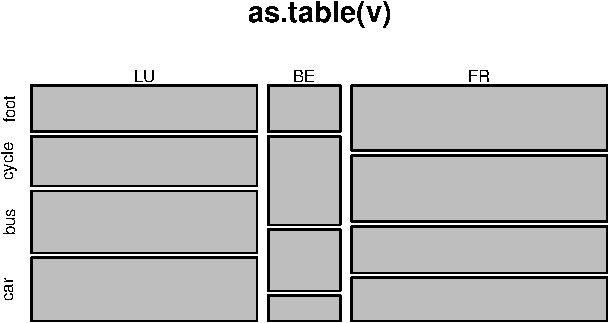
\includegraphics{065_hypotheses_contingency_files/figure-pdf/unnamed-chunk-2-1.pdf}

The chi-square test (applicable to the matrix ot to to the table) is
returned as follows:

\begin{Shaded}
\begin{Highlighting}[]
\FunctionTok{chisq.test}\NormalTok{(v)}
\CommentTok{\#\textgreater{} }
\CommentTok{\#\textgreater{}  Pearson\textquotesingle{}s Chi{-}squared test}
\CommentTok{\#\textgreater{} }
\CommentTok{\#\textgreater{} data:  v}
\CommentTok{\#\textgreater{} X{-}squared = 39.658, df = 6, p{-}value = 5.317e{-}07}
\end{Highlighting}
\end{Shaded}

The null hypothesis is that the joint distribution of the cell counts is
the product of the row and column marginal proportions.

In addition to the test itself, the function returns the sample and the
expected joint distributions:

\begin{Shaded}
\begin{Highlighting}[]
\NormalTok{G}\OtherTok{\textless{}{-}}\FunctionTok{chisq.test}\NormalTok{(v)}
\NormalTok{G}\SpecialCharTok{$}\NormalTok{observed}
\CommentTok{\#\textgreater{}    foot cycle bus car}
\CommentTok{\#\textgreater{} LU   85    92 115 117}
\CommentTok{\#\textgreater{} BE   27    52  36  15}
\CommentTok{\#\textgreater{} FR  136   139  97  91}
\NormalTok{G}\SpecialCharTok{$}\NormalTok{expected}
\CommentTok{\#\textgreater{}         foot     cycle       bus       car}
\CommentTok{\#\textgreater{} LU 101.22954 115.51597 101.22954  91.02495}
\CommentTok{\#\textgreater{} BE  32.17565  36.71657  32.17565  28.93214}
\CommentTok{\#\textgreater{} FR 114.59481 130.76747 114.59481 103.04291}
\end{Highlighting}
\end{Shaded}

The observed matrix is the one we provided and the expected matrix is
simply the multiplication of the two margin proportions for each item,
multiplied by n to turn proportions into occurrences:

\begin{Shaded}
\begin{Highlighting}[]
\FunctionTok{rowSums}\NormalTok{(v)}\SpecialCharTok{/}\NormalTok{n}
\CommentTok{\#\textgreater{}    LU    BE    FR }
\CommentTok{\#\textgreater{} 0.409 0.130 0.463}
\FunctionTok{colSums}\NormalTok{(v)}\SpecialCharTok{/}\NormalTok{n}
\CommentTok{\#\textgreater{}  foot cycle   bus   car }
\CommentTok{\#\textgreater{} 0.248 0.283 0.248 0.223}
\end{Highlighting}
\end{Shaded}

For example the number of car drivers from France is expected to be

\begin{Shaded}
\begin{Highlighting}[]
\NormalTok{n}\SpecialCharTok{*}\NormalTok{(}\FunctionTok{rowSums}\NormalTok{(v)}\SpecialCharTok{/}\NormalTok{n)[}\DecValTok{3}\NormalTok{]}\SpecialCharTok{*}\NormalTok{(}\FunctionTok{colSums}\NormalTok{(v)}\SpecialCharTok{/}\NormalTok{n)[}\DecValTok{4}\NormalTok{]}
\CommentTok{\#\textgreater{}      FR }
\CommentTok{\#\textgreater{} 103.249}
\end{Highlighting}
\end{Shaded}

We can thus see that a chi-square test is simply an answer to ``Knowing
the marginal proportions, what count can you expect for each item ?''
and then ``Is the total difference over all items a significant one?''
In the case the observed counts per cell differ from the expected based
on marginal proportions, it does mean that one or several categories of
one variable is affected by the categories of the other variable,
e.g.~transportation mode is not independent from the country of origin.

In addition to the test, the observed and epected counts, the function
also returns the residual. The residual is the difference between
observed and expected counts in each cell, but is divided by the square
root of the expected value. Since you expect that difference to be
larger for a larger occurrence you actually want to get rid of that size
effect with this division and better compare cells whether they have a
high or low expectation.

Note that in the case of smaller samples, expected values will get
smaller as well. The \texttt{chi-square()} function will not be
considered safe and returns a warning as soon one cell is expected to be
less than 5.

See for example the output with a smaller sample, while keeping the same
observed proportions:

\begin{Shaded}
\begin{Highlighting}[]
\NormalTok{n2}\OtherTok{\textless{}{-}}\DecValTok{100}
\FunctionTok{set.seed}\NormalTok{(}\DecValTok{15}\NormalTok{)}
\NormalTok{v2}\OtherTok{\textless{}{-}}\FunctionTok{matrix}\NormalTok{(}\FunctionTok{round}\NormalTok{(n2}\SpecialCharTok{*}\NormalTok{p}\SpecialCharTok{/}\FunctionTok{sum}\NormalTok{(p)),}\AttributeTok{ncol=}\DecValTok{4}\NormalTok{)}
\FunctionTok{rownames}\NormalTok{(v2)}\OtherTok{\textless{}{-}}\FunctionTok{c}\NormalTok{(}\StringTok{"LU"}\NormalTok{,}\StringTok{"BE"}\NormalTok{,}\StringTok{"FR"}\NormalTok{)}
\FunctionTok{colnames}\NormalTok{(v2)}\OtherTok{\textless{}{-}}\FunctionTok{c}\NormalTok{(}\StringTok{"foot"}\NormalTok{,}\StringTok{"cycle"}\NormalTok{,}\StringTok{"bus"}\NormalTok{,}\StringTok{"car"}\NormalTok{)}
\FunctionTok{addmargins}\NormalTok{(v2)}
\CommentTok{\#\textgreater{}     foot cycle bus car Sum}
\CommentTok{\#\textgreater{} LU     8     9  11  12  40}
\CommentTok{\#\textgreater{} BE     3     5   4   1  13}
\CommentTok{\#\textgreater{} FR    14    14  10   9  47}
\CommentTok{\#\textgreater{} Sum   25    28  25  22 100}
\NormalTok{G2}\OtherTok{\textless{}{-}}\FunctionTok{chisq.test}\NormalTok{(v2)}
\CommentTok{\#\textgreater{} Warning in chisq.test(v2): Chi{-}squared approximation may be incorrect}
\end{Highlighting}
\end{Shaded}

You see that several cells are expected to be below 5:

\begin{Shaded}
\begin{Highlighting}[]
\NormalTok{G2}\SpecialCharTok{$}\NormalTok{expected}
\CommentTok{\#\textgreater{}     foot cycle   bus   car}
\CommentTok{\#\textgreater{} LU 10.00 11.20 10.00  8.80}
\CommentTok{\#\textgreater{} BE  3.25  3.64  3.25  2.86}
\CommentTok{\#\textgreater{} FR 11.75 13.16 11.75 10.34}
\end{Highlighting}
\end{Shaded}

And the conclusion drawn from the small sample is different than with
the large one, since we cannot now reject the null hypothesis and must
conclude that transportation is independent from the country of origin.

\begin{Shaded}
\begin{Highlighting}[]
\NormalTok{G}
\CommentTok{\#\textgreater{} }
\CommentTok{\#\textgreater{}  Pearson\textquotesingle{}s Chi{-}squared test}
\CommentTok{\#\textgreater{} }
\CommentTok{\#\textgreater{} data:  v}
\CommentTok{\#\textgreater{} X{-}squared = 39.658, df = 6, p{-}value = 5.317e{-}07}
\NormalTok{G2}
\CommentTok{\#\textgreater{} }
\CommentTok{\#\textgreater{}  Pearson\textquotesingle{}s Chi{-}squared test}
\CommentTok{\#\textgreater{} }
\CommentTok{\#\textgreater{} data:  v2}
\CommentTok{\#\textgreater{} X{-}squared = 4.9246, df = 6, p{-}value = 0.5535}
\end{Highlighting}
\end{Shaded}

In such circumstances where you see that the Belgian cases were too few,
it may make sense to aggregate some levels. Let's group Belgians and
Luxembourgers together:

\begin{Shaded}
\begin{Highlighting}[]
\NormalTok{vgr}\OtherTok{\textless{}{-}}\NormalTok{v2  }\CommentTok{\#copy previous table}
\NormalTok{vgr[}\DecValTok{1}\NormalTok{,]}\OtherTok{\textless{}{-}}\NormalTok{vgr[}\DecValTok{2}\NormalTok{,]}\SpecialCharTok{+}\NormalTok{vgr[}\DecValTok{1}\NormalTok{,] }\CommentTok{\#sum BE and LU into first row}
\NormalTok{vgr}\OtherTok{\textless{}{-}}\NormalTok{vgr[}\FunctionTok{c}\NormalTok{(}\DecValTok{1}\NormalTok{,}\DecValTok{3}\NormalTok{),] }\CommentTok{\#keep only first row (BE+LU) and FR row}
\FunctionTok{rownames}\NormalTok{(vgr)}\OtherTok{\textless{}{-}}\FunctionTok{c}\NormalTok{(}\StringTok{"BE+LU"}\NormalTok{,}\StringTok{"FR"}\NormalTok{) }\CommentTok{\#adapt name}
\end{Highlighting}
\end{Shaded}

Which turns the chi squared test into a valid one this time:

\begin{Shaded}
\begin{Highlighting}[]
\NormalTok{G3}\OtherTok{\textless{}{-}}\FunctionTok{chisq.test}\NormalTok{(vgr)}
\NormalTok{G3}
\CommentTok{\#\textgreater{} }
\CommentTok{\#\textgreater{}  Pearson\textquotesingle{}s Chi{-}squared test}
\CommentTok{\#\textgreater{} }
\CommentTok{\#\textgreater{} data:  vgr}
\CommentTok{\#\textgreater{} X{-}squared = 1.7335, df = 3, p{-}value = 0.6295}
\NormalTok{G3}\SpecialCharTok{$}\NormalTok{expected}
\CommentTok{\#\textgreater{}        foot cycle   bus   car}
\CommentTok{\#\textgreater{} BE+LU 13.25 14.84 13.25 11.66}
\CommentTok{\#\textgreater{} FR    11.75 13.16 11.75 10.34}
\end{Highlighting}
\end{Shaded}

Still, given the small sample, you see the null hypothesis can't be
rejected (but the chi.square test is relevant now)

\section{Exercise}\label{exercise}

Explore a number of cross-tabulation tables from the Luxembourg2021
(census) data folder.

\chapter{Normality Test}\label{normality-test}

\section{Shapiro-Wilk Test}\label{shapiro-wilk-test}

\textbf{Testing}: \(H_0: X\) is normally distributed

The Shapiro-Wilk test assess how well an observed variable fits a normal
distribution. It is similar to testing the correlation between the
ordered sample values and the expected ones from a normal distribution.

It computes a W statistic, which measures how well the ordered sample
values match the expected values from the normal distribution. If they
don't correlate well, the W statistic is significantly lower than
expected and the null hypothesis of normality is rejected.

\section{Basic example.}\label{basic-example.}

Suppose a data of 10 values. We are not quite sure they are normally
distributed after looking at the histogram or the qq plot against a
normal distribution (\texttt{qqnorm()})

\begin{Shaded}
\begin{Highlighting}[]
\NormalTok{data }\OtherTok{\textless{}{-}} \FunctionTok{c}\NormalTok{(}\DecValTok{5}\NormalTok{, }\DecValTok{7}\NormalTok{, }\DecValTok{8}\NormalTok{, }\DecValTok{9}\NormalTok{, }\DecValTok{11}\NormalTok{, }\DecValTok{10}\NormalTok{, }\DecValTok{7}\NormalTok{, }\DecValTok{8}\NormalTok{, }\DecValTok{9}\NormalTok{, }\DecValTok{11}\NormalTok{)}
\NormalTok{n}\OtherTok{\textless{}{-}}\FunctionTok{length}\NormalTok{(data)}

\FunctionTok{hist}\NormalTok{(data)}
\end{Highlighting}
\end{Shaded}

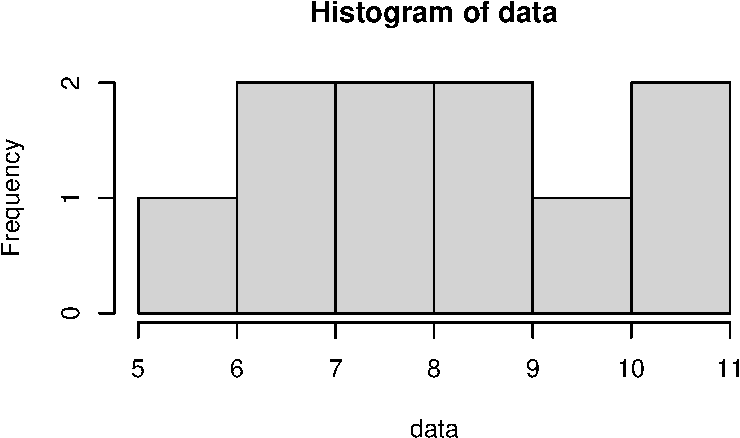
\includegraphics{066_hypotheses_normality_files/figure-pdf/unnamed-chunk-1-1.pdf}

\begin{Shaded}
\begin{Highlighting}[]
\FunctionTok{qqnorm}\NormalTok{(data)}
\end{Highlighting}
\end{Shaded}

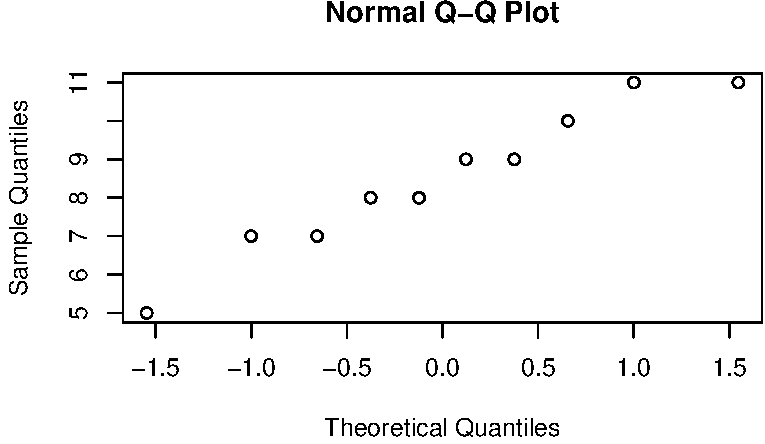
\includegraphics{066_hypotheses_normality_files/figure-pdf/unnamed-chunk-1-2.pdf}

We perform a shapiro-wilk test as follows:

\begin{Shaded}
\begin{Highlighting}[]
\FunctionTok{shapiro.test}\NormalTok{(data)}
\CommentTok{\#\textgreater{} }
\CommentTok{\#\textgreater{}  Shapiro{-}Wilk normality test}
\CommentTok{\#\textgreater{} }
\CommentTok{\#\textgreater{} data:  data}
\CommentTok{\#\textgreater{} W = 0.95259, p{-}value = 0.6992}
\end{Highlighting}
\end{Shaded}

showing we can't reject the null hypothesis. There is no significant
evidence against the data being normally distributed.

\section{Decomposing Shapiro-wilk
test}\label{decomposing-shapiro-wilk-test}

We have seen earlier that an approach to check normality could be to use
a chi-squared test after binning and checking observed counts and
expected counts along a normal distribution (goodness of fit
chi-squared). The approach of Shapiro-Wilk is technically closer to a
correlation coefficient. See how the W statistic is obtained:

First, the data is sorted and deviations to the mean computed:

\begin{Shaded}
\begin{Highlighting}[]
\NormalTok{n }\OtherTok{\textless{}{-}} \FunctionTok{length}\NormalTok{(data)}
\NormalTok{sorted\_data }\OtherTok{\textless{}{-}} \FunctionTok{sort}\NormalTok{(data)}
\NormalTok{dev\_sort}\OtherTok{\textless{}{-}}\NormalTok{sorted\_data}\SpecialCharTok{{-}}\FunctionTok{mean}\NormalTok{(data)}
\NormalTok{dev\_sort}
\CommentTok{\#\textgreater{}  [1] {-}3.5 {-}1.5 {-}1.5 {-}0.5 {-}0.5  0.5  0.5  1.5  2.5  2.5}
\end{Highlighting}
\end{Shaded}

Second, expected values from a standard normal distribution are computed
based on \texttt{qnorm()} function:

\begin{Shaded}
\begin{Highlighting}[]
\FunctionTok{qnorm}\NormalTok{((}\DecValTok{1}\SpecialCharTok{:}\NormalTok{n) }\SpecialCharTok{/}\NormalTok{ (n))}
\CommentTok{\#\textgreater{}  [1] {-}1.2815516 {-}0.8416212 {-}0.5244005 {-}0.2533471  0.0000000  0.2533471}
\CommentTok{\#\textgreater{}  [7]  0.5244005  0.8416212  1.2815516        Inf}

\NormalTok{expected\_vals }\OtherTok{\textless{}{-}} \FunctionTok{qnorm}\NormalTok{((}\DecValTok{1}\SpecialCharTok{:}\NormalTok{n }\SpecialCharTok{{-}} \FloatTok{0.375}\NormalTok{) }\SpecialCharTok{/}\NormalTok{ (n }\SpecialCharTok{+} \FloatTok{0.25}\NormalTok{))}
\NormalTok{expected\_vals}
\CommentTok{\#\textgreater{}  [1] {-}1.5466353 {-}1.0004905 {-}0.6554235 {-}0.3754618 {-}0.1225808  0.1225808}
\CommentTok{\#\textgreater{}  [7]  0.3754618  0.6554235  1.0004905  1.5466353}
\end{Highlighting}
\end{Shaded}

As you can see the values are not exactly those from the
\texttt{qnorm()} function to avoid an infinity and to correct for small
sample size (see the addition of -0.375 and 0.25 terms)

Those expected values are then scaled after the sum of squares (and the
units become irrelevant) to make expected weights

\begin{Shaded}
\begin{Highlighting}[]
\NormalTok{weights }\OtherTok{\textless{}{-}}\NormalTok{ expected\_vals }\SpecialCharTok{/} \FunctionTok{sqrt}\NormalTok{(}\FunctionTok{sum}\NormalTok{(expected\_vals}\SpecialCharTok{\^{}}\DecValTok{2}\NormalTok{))}
\end{Highlighting}
\end{Shaded}

Then those weights are multiplied by the observed deviations to the
mean. This cross-product (see numerator) is where it is similar to a
correlation coefficient: if both observed and expected vary together the
value is high:

\begin{Shaded}
\begin{Highlighting}[]
\NormalTok{numerator }\OtherTok{\textless{}{-}} \FunctionTok{sum}\NormalTok{(weights }\SpecialCharTok{*}\NormalTok{ dev\_sort)}\SpecialCharTok{\^{}}\DecValTok{2}
\NormalTok{denominator }\OtherTok{\textless{}{-}} \FunctionTok{sum}\NormalTok{(dev\_sort}\SpecialCharTok{\^{}}\DecValTok{2}\NormalTok{)}
\NormalTok{W}\OtherTok{\textless{}{-}}\NormalTok{numerator}\SpecialCharTok{/}\NormalTok{denominator}
\NormalTok{W}
\CommentTok{\#\textgreater{} [1] 0.9587322}
\end{Highlighting}
\end{Shaded}

\section{Example:}\label{example-13}

\begin{Shaded}
\begin{Highlighting}[]
\FunctionTok{library}\NormalTok{(AER)}
\CommentTok{\#\textgreater{} Error in library(AER): there is no package called \textquotesingle{}AER\textquotesingle{}}
\FunctionTok{data}\NormalTok{(Parade2005)}
\CommentTok{\#\textgreater{} Warning in data(Parade2005): data set \textquotesingle{}Parade2005\textquotesingle{} not found}
\FunctionTok{attach}\NormalTok{(Parade2005)}
\CommentTok{\#\textgreater{} Error: object \textquotesingle{}Parade2005\textquotesingle{} not found}

\FunctionTok{shapiro.test}\NormalTok{(earnings)}
\CommentTok{\#\textgreater{} Error: object \textquotesingle{}earnings\textquotesingle{} not found}
\FunctionTok{shapiro.test}\NormalTok{(}\FunctionTok{log}\NormalTok{(earnings))}
\CommentTok{\#\textgreater{} Error: object \textquotesingle{}earnings\textquotesingle{} not found}
\FunctionTok{shapiro.test}\NormalTok{(earnings[celebrity}\SpecialCharTok{==}\StringTok{\textquotesingle{}no\textquotesingle{}}\NormalTok{])}
\CommentTok{\#\textgreater{} Error: object \textquotesingle{}earnings\textquotesingle{} not found}

\FunctionTok{qqnorm}\NormalTok{(}\FunctionTok{scale}\NormalTok{(earnings))}
\CommentTok{\#\textgreater{} Error: object \textquotesingle{}earnings\textquotesingle{} not found}
\FunctionTok{qqnorm}\NormalTok{(}\FunctionTok{scale}\NormalTok{(earnings[earnings }\SpecialCharTok{\textless{}} \DecValTok{100000}\NormalTok{]))}
\CommentTok{\#\textgreater{} Error: object \textquotesingle{}earnings\textquotesingle{} not found}
\end{Highlighting}
\end{Shaded}

\chapter{Power analysis - contingency
table}\label{power-analysis---contingency-table}

While designing a research including an experiment, you regularly find
yourself in the need to balance your own time or personal resource with
the number of factors for which you can test an interaction. This
regularly boils down to minimizing the number of participants
(especially when your guinea pigs are your fellow students) in your
experience while ensuring you can still identify an effect, an
interdependence between your factors if any. This search is generally
called a \textbf{power analysis}. It is essentially reversing the
previous approach where you identify the probability of rejecting the
null hypothesis given a certain number of observations. Here you fix the
rejection probability in order to find a minimum number of observations.

We demonstrate a power analysis in the case of a chi-squared test of
independence but similar power test exist for the other tests we have
seen earlier. We will use the \texttt{pwr} R package for this analysis.

\section{Example}\label{example-14}

We have two categorical variables, A and B, with the following marginal
proportions: - Variable A: 3 categories (A1, A2, A3), e.g.~``rural'',
``urban'', ``suburban'') - Variable B: 2 categories (B1, B2), e.g.~``not
vegeterian'', ``vegetarian''

In the population we know that freqeuncies are not homogeneously
distributed across the categories. Suppose the following marginal
proportions. They are typically known form a census of residential
places and a nation-wide study of vegetarianism:

\begin{itemize}
\tightlist
\item
  \(P(A1) = 0.3\)
\item
  \(P(A2) = 0.4\)
\item
  \(P(A3) = 0.3\)
\item
  \(P(B1) = 0.8\)
\item
  \(P(B2) = 0.2\)
\end{itemize}

Our goal is to find the minmum total sample size \(N\) needed for a link
between A and B, i.e.~urbanity and vegetarianism to be detected. From
\(N\) and the proportions of the A variable (rural, urban or suburban
people), we can then invite a relevant number of participants based on
their residential place.

\section{Power analysis elements}\label{power-analysis-elements}

The power analysis will determine the sample size required to detect an
effect of \emph{a given size} with \emph{a given degree of confidence}.
It requires you to define three parameters, one of which i salpha which
we know already well:

\begin{itemize}
\item
  \textbf{Power ((1-\beta))}: the probability that the test will
  correctly reject the null hypothesis when the alternative hypothesis
  is true (see type of errors). A power of 0.80 is commonly used,
  meaning there is an 80\% chance of detecting a true effect.
\item
  \textbf{Significance Level ((\alpha))}: the probability of rejecting
  the null hypothesis when it is actually true (Type I error). Again we
  can use the typical value of 0.05.
\item
  \textbf{Effect Size}: this is a measure of the magnitude of the
  phenomenon we want to be able to identify. In chi-square tests,
  Cohen's \(w\) is often used to quantify this effect size. Cohen's
  \(w\) is easily calculated from the chi-squared statistics applied to
  the contingency table. It is defined as
\end{itemize}

\[w = \sqrt{\frac{\chi^2}{N}}\]

where \(\chi^2\) is the chi-square statistic and \(N\) is the total
sample size.

A standard approach is to fix Cohen's \(w=0.3\), which is said to be a
medium effect. We then see that if \(w\) is fixed we obtain \(N\) from
the \(\chi^2\):

\[N = \sqrt{\frac{\chi^2}{w}}\] \#\# Implementation

First we load the power analysis package \texttt{pwr} and define our
parameters:

\begin{Shaded}
\begin{Highlighting}[]
\FunctionTok{library}\NormalTok{(pwr)}
\CommentTok{\#\textgreater{} Error in library(pwr): there is no package called \textquotesingle{}pwr\textquotesingle{}}

\CommentTok{\# Define the parameters}
\NormalTok{power }\OtherTok{\textless{}{-}} \FloatTok{0.80} \CommentTok{\# Desired power level}
\NormalTok{effectw }\OtherTok{\textless{}{-}} \FloatTok{0.3} \CommentTok{\# Medium effect size Cohen w}
\NormalTok{alpha }\OtherTok{\textless{}{-}} \FloatTok{0.05} \CommentTok{\# Significance level}

\NormalTok{df }\OtherTok{\textless{}{-}} \DecValTok{2} \CommentTok{\# Degrees of freedom for a 3x2 table, i.e (3{-}1)(2{-}1)=2}
\end{Highlighting}
\end{Shaded}

Second, we compute the power based on the chi-squared test:

\begin{Shaded}
\begin{Highlighting}[]
\FunctionTok{pwr.chisq.test}\NormalTok{(}\AttributeTok{w =}\NormalTok{ effectw, }\AttributeTok{df =}\NormalTok{ df, }\AttributeTok{sig.level =}\NormalTok{ alpha, }\AttributeTok{power =}\NormalTok{ power)}
\CommentTok{\#\textgreater{} Error in pwr.chisq.test(w = effectw, df = df, sig.level = alpha, power = power): could not find function "pwr.chisq.test"}
\end{Highlighting}
\end{Shaded}

The output indicates the total sample size required to achieve the
desired power and effect size.

The above doesn't make use of the observed margins proportions which we
use simply now to allocate the total sample size according to the
proportions for each category of variable A, that is a
\textbf{stratified sampling}:

\begin{Shaded}
\begin{Highlighting}[]
\NormalTok{pwrresult}\OtherTok{\textless{}{-}}\FunctionTok{pwr.chisq.test}\NormalTok{(}\AttributeTok{w =}\NormalTok{ effectw, }\AttributeTok{df =}\NormalTok{ df, }\AttributeTok{sig.level =}\NormalTok{ alpha, }\AttributeTok{power =}\NormalTok{ power)}
\CommentTok{\#\textgreater{} Error in pwr.chisq.test(w = effectw, df = df, sig.level = alpha, power = power): could not find function "pwr.chisq.test"}

\FunctionTok{ceiling}\NormalTok{(pwrresult}\SpecialCharTok{$}\NormalTok{N}\SpecialCharTok{*}\FunctionTok{c}\NormalTok{(}\AttributeTok{A1=}\FloatTok{0.3}\NormalTok{,}\AttributeTok{A2=}\FloatTok{0.4}\NormalTok{,}\AttributeTok{A3=}\FloatTok{0.3}\NormalTok{))}
\CommentTok{\#\textgreater{} Error: object \textquotesingle{}pwrresult\textquotesingle{} not found}
\end{Highlighting}
\end{Shaded}

\section{Effect size and degrees of
freedom}\label{effect-size-and-degrees-of-freedom}

With alpha being set at 0.05 and the pover level 1-beta set to 0.80, we
can cross-tabulate the effect size \(w\) against the degrees of freedom
to get an idea of the effect of being more or less demanding and the
effect of aggregating/subdividing categories:

\begin{Shaded}
\begin{Highlighting}[]
\NormalTok{dfs}\OtherTok{\textless{}{-}}\DecValTok{1}\SpecialCharTok{:}\DecValTok{6}
\NormalTok{ws}\OtherTok{\textless{}{-}}\FunctionTok{seq}\NormalTok{(}\FloatTok{0.2}\NormalTok{,}\FloatTok{0.5}\NormalTok{, }\AttributeTok{by=}\FloatTok{0.05}\NormalTok{)}
\NormalTok{D}\OtherTok{\textless{}{-}}\FunctionTok{data.frame}\NormalTok{(}\AttributeTok{df=}\FunctionTok{rep}\NormalTok{(dfs, }\AttributeTok{each=}\FunctionTok{length}\NormalTok{(ws)),}\AttributeTok{w=}\FunctionTok{rep}\NormalTok{(ws,}\FunctionTok{length}\NormalTok{(dfs)))}

\NormalTok{D}\SpecialCharTok{$}\NormalTok{N}\OtherTok{\textless{}{-}}\FunctionTok{apply}\NormalTok{(D, }\DecValTok{1}\NormalTok{, }\ControlFlowTok{function}\NormalTok{(x)\{}
\NormalTok{  pwrresult}\OtherTok{\textless{}{-}}\FunctionTok{pwr.chisq.test}\NormalTok{(}\AttributeTok{w =}\NormalTok{ x[}\DecValTok{2}\NormalTok{], }\AttributeTok{df =}\NormalTok{ x[}\DecValTok{1}\NormalTok{],}
                 \AttributeTok{sig.level =} \FloatTok{0.05}\NormalTok{, }\AttributeTok{power =} \FloatTok{0.8}\NormalTok{)}
  \FunctionTok{ceiling}\NormalTok{(pwrresult}\SpecialCharTok{$}\NormalTok{N)}
\NormalTok{  \})}
\CommentTok{\#\textgreater{} Error in pwr.chisq.test(w = x[2], df = x[1], sig.level = 0.05, power = 0.8): could not find function "pwr.chisq.test"}
\NormalTok{D}
\CommentTok{\#\textgreater{}    df    w}
\CommentTok{\#\textgreater{} 1   1 0.20}
\CommentTok{\#\textgreater{} 2   1 0.25}
\CommentTok{\#\textgreater{} 3   1 0.30}
\CommentTok{\#\textgreater{} 4   1 0.35}
\CommentTok{\#\textgreater{} 5   1 0.40}
\CommentTok{\#\textgreater{} 6   1 0.45}
\CommentTok{\#\textgreater{} 7   1 0.50}
\CommentTok{\#\textgreater{} 8   2 0.20}
\CommentTok{\#\textgreater{} 9   2 0.25}
\CommentTok{\#\textgreater{} 10  2 0.30}
\CommentTok{\#\textgreater{} 11  2 0.35}
\CommentTok{\#\textgreater{} 12  2 0.40}
\CommentTok{\#\textgreater{} 13  2 0.45}
\CommentTok{\#\textgreater{} 14  2 0.50}
\CommentTok{\#\textgreater{} 15  3 0.20}
\CommentTok{\#\textgreater{} 16  3 0.25}
\CommentTok{\#\textgreater{} 17  3 0.30}
\CommentTok{\#\textgreater{} 18  3 0.35}
\CommentTok{\#\textgreater{} 19  3 0.40}
\CommentTok{\#\textgreater{} 20  3 0.45}
\CommentTok{\#\textgreater{} 21  3 0.50}
\CommentTok{\#\textgreater{} 22  4 0.20}
\CommentTok{\#\textgreater{} 23  4 0.25}
\CommentTok{\#\textgreater{} 24  4 0.30}
\CommentTok{\#\textgreater{} 25  4 0.35}
\CommentTok{\#\textgreater{} 26  4 0.40}
\CommentTok{\#\textgreater{} 27  4 0.45}
\CommentTok{\#\textgreater{} 28  4 0.50}
\CommentTok{\#\textgreater{} 29  5 0.20}
\CommentTok{\#\textgreater{} 30  5 0.25}
\CommentTok{\#\textgreater{} 31  5 0.30}
\CommentTok{\#\textgreater{} 32  5 0.35}
\CommentTok{\#\textgreater{} 33  5 0.40}
\CommentTok{\#\textgreater{} 34  5 0.45}
\CommentTok{\#\textgreater{} 35  5 0.50}
\CommentTok{\#\textgreater{} 36  6 0.20}
\CommentTok{\#\textgreater{} 37  6 0.25}
\CommentTok{\#\textgreater{} 38  6 0.30}
\CommentTok{\#\textgreater{} 39  6 0.35}
\CommentTok{\#\textgreater{} 40  6 0.40}
\CommentTok{\#\textgreater{} 41  6 0.45}
\CommentTok{\#\textgreater{} 42  6 0.50}
\end{Highlighting}
\end{Shaded}

Graphically:

\begin{Shaded}
\begin{Highlighting}[]
\FunctionTok{library}\NormalTok{(ggplot2)}
\FunctionTok{library}\NormalTok{(scales)}

\FunctionTok{ggplot}\NormalTok{(}\AttributeTok{data=}\NormalTok{D)}\SpecialCharTok{+}
  \FunctionTok{geom\_line}\NormalTok{(}\FunctionTok{aes}\NormalTok{(}\AttributeTok{x=}\NormalTok{df,}\AttributeTok{y=}\NormalTok{N, }\AttributeTok{group=}\FunctionTok{factor}\NormalTok{(w), }\AttributeTok{col=}\NormalTok{w))}\SpecialCharTok{+}
  \FunctionTok{theme\_bw}\NormalTok{()}
\CommentTok{\#\textgreater{} Error in \textasciigrave{}geom\_line()\textasciigrave{}:}
\CommentTok{\#\textgreater{} ! Problem while computing aesthetics.}
\CommentTok{\#\textgreater{} i Error occurred in the 1st layer.}
\CommentTok{\#\textgreater{} Caused by error:}
\CommentTok{\#\textgreater{} ! object \textquotesingle{}N\textquotesingle{} not found}
\end{Highlighting}
\end{Shaded}

Or a two entries table to find N

\begin{Shaded}
\begin{Highlighting}[]
\NormalTok{reshape2}\SpecialCharTok{::}\FunctionTok{dcast}\NormalTok{(D, df }\SpecialCharTok{\textasciitilde{}}\NormalTok{ w, }\AttributeTok{value.var=}\StringTok{"N"}\NormalTok{)}
\CommentTok{\#\textgreater{} Error: value.var (N) not found in input}
\end{Highlighting}
\end{Shaded}

\part{Part VII - Bivariate and regression analysis}

\chapter{Correlation and regression}\label{correlation-and-regression}

The relationship between two processes (variables) that vary in space
can be assessed visually through comparing maps. While maps are
important geographical instruments, correlation and regression analyses
can make the visual association more precise by defining:

\begin{itemize}
\tightlist
\item
  \textbf{How strong the association is}
\item
  \textbf{What form of association it is}
\end{itemize}

Maps are still very useful in suggesting processes to be associated and
to identify new attributes for complementing correlation-regression
(analysis of residuals)

\section{Double objective:}\label{double-objective}

\begin{enumerate}
\def\labelenumi{\arabic{enumi}.}
\tightlist
\item
  \textbf{Explaining} the spatial distribution of a process using
  another or several other processes.
\end{enumerate}

\begin{itemize}
\tightlist
\item
  A \textbf{correlation} examines the \textbf{degree of association} (no
  direction of causality)
\item
  A \textbf{regression} identifies a process to be explained,
  represented by a \textbf{dependent variable} and one or several
  explanatory processes, the \textbf{independent variables}
\end{itemize}

\textbf{\emph{Correlation comes first, it is more exploratory}}

\begin{enumerate}
\def\labelenumi{\arabic{enumi}.}
\setcounter{enumi}{1}
\tightlist
\item
  \textbf{Predicting}the spatial distribution of a process \(Y\), given
  the spatial distribution of an associated process \(X\)
\end{enumerate}

\begin{itemize}
\tightlist
\item
  \textbf{Not necessarily looking for explanations}
\item
  But predicting with a \textbf{measured precision}
\end{itemize}

\section{Covariation, Covariance and
Correlation}\label{covariation-covariance-and-correlation}

Let \(X\) and \(Y\) be - cardinal (ratio) numeric variables - varying
across space, i.e.~in every \(i\) of \(n\) places

\textbf{To what degree do the two variables vary together ?}

\textbf{To what degree are they interdependent ?}

Let's define:

\begin{itemize}
\item
  Mean: \(\bar{X}\), \(\bar{Y}\)
\item
  Deviation to the mean: \(x_i = X_i - \hat{X}\) and
  \(y_i = Y_i - \hat{Y}\)
\item
  \textbf{Covariation}: sum over each place of the product of the
  deviations in \(X\) and \(Y\).
  \[Covariation (X,Y) = \sum_{i=1}^n x_i y_i\]
\end{itemize}

The idea of a covariation is to create a value that increases when
observations vary `together' along the two variables. If an observation
i is just above the mean in X but far above the mean in Y, the product
is rather small. But if is far from the mean in both X and Y the product
of both is very high. However, everything else equal, covariation
increases with the number of observations

\begin{itemize}
\tightlist
\item
  \textbf{Covariance}: \[Cov(X,Y) = \dfrac {\sum_{i=1}^n x_i y_i} {n}\]
\end{itemize}

The covariance embeds the same idea as the covariation but resolves the
issue of sample size with \(n\) at the denominator. Two samples of the
same two variables can thus be compared even if they have different
numbers of observations.

However, if those two samples have different dispersion (e.g.~weight
measured over a different range of ages), the one with the larger
dispersion will still have a larger covariance and impact our
understanding of how \(X\) and \(Y\) are related.

\begin{itemize}
\tightlist
\item
  \textbf{Correlation} coefficient (Pearson\ldots{} no assumption on
  random distribution):
  \[\rho_{XY} = \dfrac {Cov(X,Y)} {\sigma_X \sigma_Y}\]
\end{itemize}

with \(\sigma_X\) and \(\sigma_Y\) the standard deviations.

The correlation resolves the issue of a different dispersion by dividing
the covariance by the product of the standard deviations. Doing so, the
measurement units also disappear, hence it is comparable even if we
would measure one of the variable using a different (linearly related)
metric. For example if we had \(X\) in {[}kg{]} and \(Y\) in {[}cm{]},
the covariance would be in {[}kg x cm{]} and not directly comparable to
another set where {[}g{]} and {[}mm{]} would be used. With the
correlation, we no longer care since we divide by the same product of
units as the denominator

\section{Correlation coefficient
characteristics}\label{correlation-coefficient-characteristics}

\begin{itemize}
\item
  is a \emph{pure} number (no units)
\item
  is \emph{invariant} to any linear transformation (including
  standardization)
\item
  indicates whether there is a \emph{linear} relationship between \(X\)
  and \(Y\).

  \[−1≤ \rho_{XY} ≤1\]
\item
  \(\rho\) is close to 1 if the slope of the line that can be drawn in
  the plot is positive
\item
  \(\rho\) is close to -1 if the slope of the line that can be drawn in
  the plot is negative
\item
  \(\rho\) is close to 0 if the plot has no particular form. \emph{Note
  that it does not mean that the variables are independent but that the
  relationship is non linear !}
\end{itemize}

\begin{Shaded}
\begin{Highlighting}[]
\FunctionTok{set.seed}\NormalTok{(}\DecValTok{123}\NormalTok{)}
\NormalTok{x}\OtherTok{\textless{}{-}}\FunctionTok{c}\NormalTok{(}\DecValTok{1}\NormalTok{,}\FloatTok{1.5}\NormalTok{,}\FloatTok{1.5}\NormalTok{,}\DecValTok{2}\NormalTok{,}\FloatTok{2.5}\NormalTok{,}\DecValTok{3}\NormalTok{,}\DecValTok{4}\NormalTok{,}\DecValTok{4}\NormalTok{,}\FloatTok{4.5}\NormalTok{,}\FloatTok{4.5}\NormalTok{,}\FloatTok{5.5}\NormalTok{,}\DecValTok{6}\NormalTok{,}\FloatTok{6.5}\NormalTok{)}
\NormalTok{y1}\OtherTok{\textless{}{-}}\FunctionTok{c}\NormalTok{(}\DecValTok{10}\NormalTok{,}\DecValTok{15}\NormalTok{,}\DecValTok{12}\NormalTok{,}\DecValTok{17}\NormalTok{,}\DecValTok{30}\NormalTok{,}\DecValTok{28}\NormalTok{,}\DecValTok{40}\NormalTok{,}\DecValTok{30}\NormalTok{,}\DecValTok{44}\NormalTok{,}\DecValTok{40}\NormalTok{,}\DecValTok{59}\NormalTok{,}\DecValTok{58}\NormalTok{,}\DecValTok{67}\NormalTok{)}
\NormalTok{y2}\OtherTok{\textless{}{-}}\FunctionTok{mean}\NormalTok{(y1)}\SpecialCharTok{+}\FunctionTok{runif}\NormalTok{(}\FunctionTok{length}\NormalTok{(y1),}\AttributeTok{min =} \SpecialCharTok{{-}}\DecValTok{30}\NormalTok{, }\AttributeTok{max=}\DecValTok{30}\NormalTok{)}
\NormalTok{y3}\OtherTok{\textless{}{-}}\DecValTok{70}\SpecialCharTok{{-}}\NormalTok{y1}
\FunctionTok{par}\NormalTok{(}\AttributeTok{mfrow =} \FunctionTok{c}\NormalTok{(}\DecValTok{1}\NormalTok{,}\DecValTok{3}\NormalTok{))}
\FunctionTok{plot}\NormalTok{(x,y1,}\AttributeTok{ylim=}\FunctionTok{c}\NormalTok{(}\DecValTok{1}\NormalTok{,}\DecValTok{70}\NormalTok{), }\AttributeTok{col=}\StringTok{"black"}\NormalTok{, }\AttributeTok{pch=}\DecValTok{16}\NormalTok{)}
\FunctionTok{plot}\NormalTok{(x,y2,}\AttributeTok{ylim=}\FunctionTok{c}\NormalTok{(}\DecValTok{1}\NormalTok{,}\DecValTok{70}\NormalTok{), }\AttributeTok{col=}\StringTok{"black"}\NormalTok{, }\AttributeTok{pch=}\DecValTok{16}\NormalTok{)}
\FunctionTok{plot}\NormalTok{(x,y3,}\AttributeTok{ylim=}\FunctionTok{c}\NormalTok{(}\DecValTok{1}\NormalTok{,}\DecValTok{70}\NormalTok{), }\AttributeTok{col=}\StringTok{"black"}\NormalTok{, }\AttributeTok{pch=}\DecValTok{16}\NormalTok{)}
\end{Highlighting}
\end{Shaded}

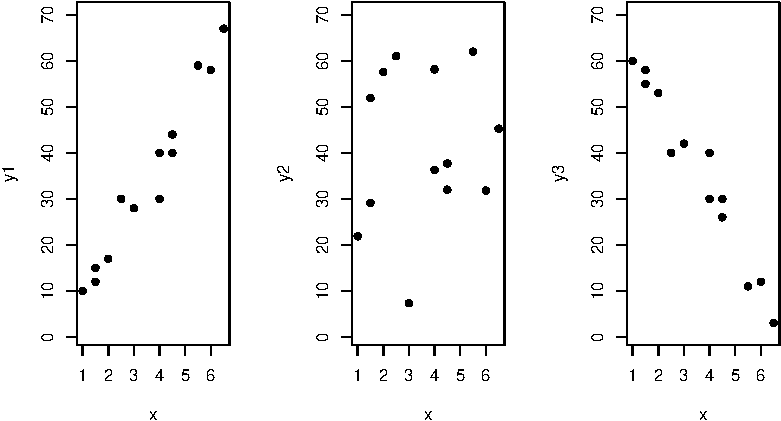
\includegraphics{071_correlation_files/figure-pdf/unnamed-chunk-1-1.pdf}

On the above figure, the correlations are respectively:

\begin{Shaded}
\begin{Highlighting}[]
\FunctionTok{cor}\NormalTok{(x,y1)}
\CommentTok{\#\textgreater{} [1] 0.9786531}
\FunctionTok{cor}\NormalTok{(x,y2)}
\CommentTok{\#\textgreater{} [1] 0.1299222}
\FunctionTok{cor}\NormalTok{(x,y3)}
\CommentTok{\#\textgreater{} [1] {-}0.9786531}
\end{Highlighting}
\end{Shaded}

See that the order of x and y doesn't matter and that if x (or y) is
added a fixed number and multiplied by another, i.e.~undergoes a linear
transformation, the correlation coefficient doesn't change

\begin{Shaded}
\begin{Highlighting}[]
\FunctionTok{cor}\NormalTok{(y1,x)}
\CommentTok{\#\textgreater{} [1] 0.9786531}
\FunctionTok{cor}\NormalTok{(}\DecValTok{5}\SpecialCharTok{+}\DecValTok{10}\SpecialCharTok{*}\NormalTok{x,y1)}
\CommentTok{\#\textgreater{} [1] 0.9786531}
\end{Highlighting}
\end{Shaded}

\section{Correlation confidence}\label{correlation-confidence}

If we have access to the total population, we know \(X\) and \(Y\) for
every individual. The population correlation coefficient is usually
denoted \(\rho_{XY}\).

Usually, however, only a sample of the population is observed. On that
sample, we can calculate \(r_{XY}\), which is an estimation of
\(\rho_{XY}\).

From \(r_{XY}\), confidence intervals can be calculated and thus
hypotheses can be tested about \(\rho_{XY}\).

Test \(H0: \rho_{XY} = 0\) (alternative: \(H1: \rho_{XY} \ne0\))

Suppose \(X\), \(Y\) follow a normal distribution (or at least one of
them).

Calculate \(t\) statistic:
\[t_0 = \dfrac {|r|\sqrt{n-2}}{\sqrt{1-r^2}} \sim t_{n-2}\] If
\(t_0 \le t_{n-2}\)

\(H0\) is rejected when \(P(t_0 \le t_{n-2}) = \alpha\).

The relevant t.test is included in the \texttt{cor.test()} function. The
test is applied to our example graphs

\begin{Shaded}
\begin{Highlighting}[]
\FunctionTok{cor.test}\NormalTok{(x,y1)}
\CommentTok{\#\textgreater{} }
\CommentTok{\#\textgreater{}  Pearson\textquotesingle{}s product{-}moment correlation}
\CommentTok{\#\textgreater{} }
\CommentTok{\#\textgreater{} data:  x and y1}
\CommentTok{\#\textgreater{} t = 15.793, df = 11, p{-}value = 6.617e{-}09}
\CommentTok{\#\textgreater{} alternative hypothesis: true correlation is not equal to 0}
\CommentTok{\#\textgreater{} 95 percent confidence interval:}
\CommentTok{\#\textgreater{}  0.9281459 0.9937728}
\CommentTok{\#\textgreater{} sample estimates:}
\CommentTok{\#\textgreater{}       cor }
\CommentTok{\#\textgreater{} 0.9786531}
\FunctionTok{cor.test}\NormalTok{(x,y2)}
\CommentTok{\#\textgreater{} }
\CommentTok{\#\textgreater{}  Pearson\textquotesingle{}s product{-}moment correlation}
\CommentTok{\#\textgreater{} }
\CommentTok{\#\textgreater{} data:  x and y2}
\CommentTok{\#\textgreater{} t = 0.43459, df = 11, p{-}value = 0.6723}
\CommentTok{\#\textgreater{} alternative hypothesis: true correlation is not equal to 0}
\CommentTok{\#\textgreater{} 95 percent confidence interval:}
\CommentTok{\#\textgreater{}  {-}0.4535291  0.6354207}
\CommentTok{\#\textgreater{} sample estimates:}
\CommentTok{\#\textgreater{}       cor }
\CommentTok{\#\textgreater{} 0.1299222}
\FunctionTok{cor.test}\NormalTok{(x,y3)}
\CommentTok{\#\textgreater{} }
\CommentTok{\#\textgreater{}  Pearson\textquotesingle{}s product{-}moment correlation}
\CommentTok{\#\textgreater{} }
\CommentTok{\#\textgreater{} data:  x and y3}
\CommentTok{\#\textgreater{} t = {-}15.793, df = 11, p{-}value = 6.617e{-}09}
\CommentTok{\#\textgreater{} alternative hypothesis: true correlation is not equal to 0}
\CommentTok{\#\textgreater{} 95 percent confidence interval:}
\CommentTok{\#\textgreater{}  {-}0.9937728 {-}0.9281459}
\CommentTok{\#\textgreater{} sample estimates:}
\CommentTok{\#\textgreater{}        cor }
\CommentTok{\#\textgreater{} {-}0.9786531}
\end{Highlighting}
\end{Shaded}

The null hypothesis is well rejected in the first and third cases. It
cannot be rejected in the second case, showing there is no correlation.

Note: using ordinal data requires other measures, e.g.~Spearman or
Kendall. These measures can be used with continuous data as well and may
help identifying data problems (strange values) or asymetric
distributions.

\chapter{Regression}\label{regression}

\section{Example}\label{example-15}

To illustrate the functioning of a regression model, we use a dataset
from Ferguson (n.d.) (table 1 and 2) representing average precipitation
and elevation across southern Scotland (between national grid lines 600
and 601 km N).

\begin{Shaded}
\begin{Highlighting}[]
\NormalTok{RainScotland}\OtherTok{\textless{}{-}}\FunctionTok{read.csv}\NormalTok{(}\StringTok{"data/Ferguson/RainScotland.csv"}\NormalTok{)}
\end{Highlighting}
\end{Shaded}


\includegraphics{data/Ferguson/RainScotland_AIGenerated_dallE3.jpg}

Our first variable of interest is \textbf{Rainfall in mm/yr} and the
second is \textbf{Elevation in m} above sea level.

Always start with a scatterplot when possible:

\begin{Shaded}
\begin{Highlighting}[]
\FunctionTok{plot}\NormalTok{(}\AttributeTok{x=}\NormalTok{RainScotland}\SpecialCharTok{$}\NormalTok{Elevation, }\AttributeTok{y=}\NormalTok{RainScotland}\SpecialCharTok{$}\NormalTok{Rainfall,}
    \AttributeTok{xlab=}\StringTok{"X : Elevation (m)"}\NormalTok{, }\AttributeTok{ylab=}\StringTok{"Y : Rainfall (mm)"}\NormalTok{,}
    \AttributeTok{xlim=}\FunctionTok{c}\NormalTok{(}\DecValTok{0}\NormalTok{,}\DecValTok{600}\NormalTok{), }\AttributeTok{ylim=}\FunctionTok{c}\NormalTok{(}\DecValTok{0}\NormalTok{,}\DecValTok{2500}\NormalTok{), }\AttributeTok{yaxs=}\StringTok{"i"}\NormalTok{, }\AttributeTok{xaxs=}\StringTok{"i"}\NormalTok{)}
\end{Highlighting}
\end{Shaded}

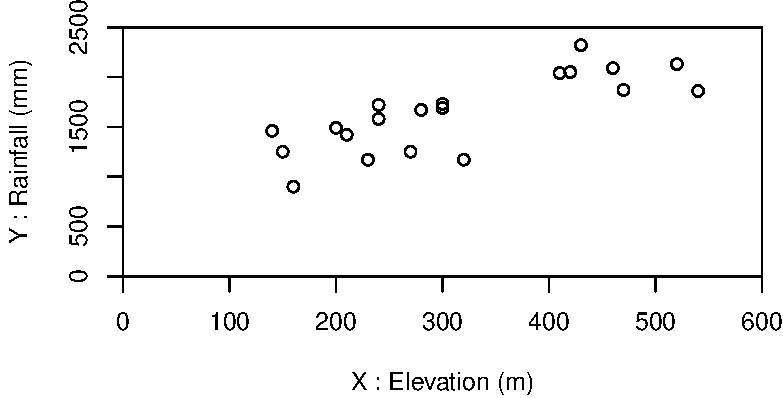
\includegraphics{072_regression_files/figure-pdf/unnamed-chunk-2-1.pdf}

We can see and measure that the two variables correlate positively and
significantly:

\begin{Shaded}
\begin{Highlighting}[]
\FunctionTok{cor}\NormalTok{(RainScotland}\SpecialCharTok{$}\NormalTok{Elevation, RainScotland}\SpecialCharTok{$}\NormalTok{Rainfall)}
\CommentTok{\#\textgreater{} [1] 0.7839175}
\FunctionTok{cor.test}\NormalTok{(RainScotland}\SpecialCharTok{$}\NormalTok{Elevation, RainScotland}\SpecialCharTok{$}\NormalTok{Rainfall)}
\CommentTok{\#\textgreater{} }
\CommentTok{\#\textgreater{}  Pearson\textquotesingle{}s product{-}moment correlation}
\CommentTok{\#\textgreater{} }
\CommentTok{\#\textgreater{} data:  RainScotland$Elevation and RainScotland$Rainfall}
\CommentTok{\#\textgreater{} t = 5.3568, df = 18, p{-}value = 4.317e{-}05}
\CommentTok{\#\textgreater{} alternative hypothesis: true correlation is not equal to 0}
\CommentTok{\#\textgreater{} 95 percent confidence interval:}
\CommentTok{\#\textgreater{}  0.5227325 0.9105639}
\CommentTok{\#\textgreater{} sample estimates:}
\CommentTok{\#\textgreater{}       cor }
\CommentTok{\#\textgreater{} 0.7839175}
\end{Highlighting}
\end{Shaded}

\section{Simple regression --
principle}\label{simple-regression-principle}

\textbf{What is the straight line that best fits this plot ?}

Let's draw one line and define the \textbf{residual}, \(e_i\), as the
vertical difference between the `best line' and the point
\((X_i, Y_i)\).

As you know a straight line is entirely defined by its slope (\(b\)) and
its intercept (\(a\)). With \(a=700\) and \(b=3\) we have quite a good
proxy:

\begin{Shaded}
\begin{Highlighting}[]
\FunctionTok{plot}\NormalTok{(}\AttributeTok{x=}\NormalTok{RainScotland}\SpecialCharTok{$}\NormalTok{Elevation, }\AttributeTok{y=}\NormalTok{RainScotland}\SpecialCharTok{$}\NormalTok{Rainfall,}
    \AttributeTok{xlab=}\StringTok{"X : Elevation (m)"}\NormalTok{, }\AttributeTok{ylab=}\StringTok{"Y : Rainfall (mm)"}\NormalTok{,}
    \AttributeTok{xlim=}\FunctionTok{c}\NormalTok{(}\DecValTok{0}\NormalTok{,}\DecValTok{600}\NormalTok{), }\AttributeTok{ylim=}\FunctionTok{c}\NormalTok{(}\DecValTok{0}\NormalTok{,}\DecValTok{2500}\NormalTok{), }\AttributeTok{yaxs=}\StringTok{"i"}\NormalTok{, }\AttributeTok{xaxs=}\StringTok{"i"}\NormalTok{)}
\NormalTok{l\_a}\OtherTok{=}\DecValTok{700}
\NormalTok{l\_b}\OtherTok{=}\DecValTok{3}
\FunctionTok{abline}\NormalTok{(}\AttributeTok{a=}\NormalTok{l\_a,}\AttributeTok{b=}\NormalTok{l\_b, }\AttributeTok{col=}\StringTok{"orange"}\NormalTok{)}
\FunctionTok{text}\NormalTok{(}\AttributeTok{x=}\NormalTok{RainScotland}\SpecialCharTok{$}\NormalTok{Elevation[}\DecValTok{18}\NormalTok{]}\SpecialCharTok{+}\DecValTok{25}\NormalTok{,}\AttributeTok{y=}\NormalTok{RainScotland}\SpecialCharTok{$}\NormalTok{Rainfall[}\DecValTok{18}\NormalTok{]}\SpecialCharTok{+}\DecValTok{100}\NormalTok{,}\AttributeTok{labels =} \StringTok{"e\_18"}\NormalTok{, }\AttributeTok{col=}\StringTok{"orange"}\NormalTok{)}
\FunctionTok{segments}\NormalTok{(}\AttributeTok{x0=}\NormalTok{RainScotland}\SpecialCharTok{$}\NormalTok{Elevation[}\DecValTok{18}\NormalTok{],}\AttributeTok{y0=}\NormalTok{RainScotland}\SpecialCharTok{$}\NormalTok{Rainfall[}\DecValTok{18}\NormalTok{],}
         \AttributeTok{x1=}\NormalTok{RainScotland}\SpecialCharTok{$}\NormalTok{Elevation[}\DecValTok{18}\NormalTok{], }\AttributeTok{y1=}\NormalTok{l\_a}\SpecialCharTok{+}\NormalTok{l\_b}\SpecialCharTok{*}\NormalTok{RainScotland}\SpecialCharTok{$}\NormalTok{Elevation[}\DecValTok{18}\NormalTok{], }\AttributeTok{col=}\StringTok{"darkorange"}\NormalTok{,}\AttributeTok{lwd=}\DecValTok{2}\NormalTok{)}
\end{Highlighting}
\end{Shaded}

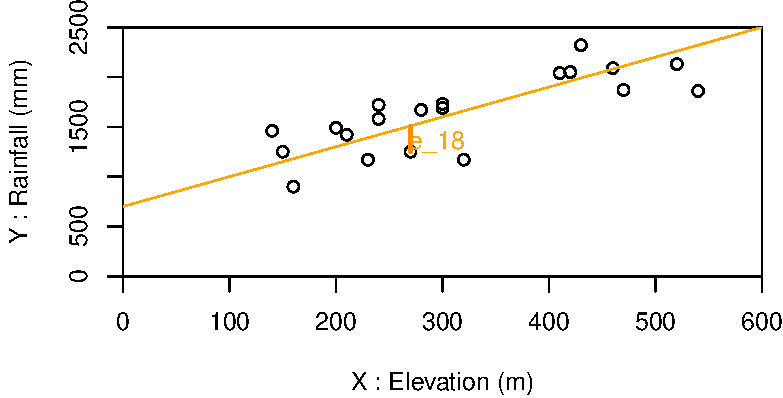
\includegraphics{072_regression_files/figure-pdf/unnamed-chunk-4-1.pdf}

There could be many lines to approximate the graph and for which
residuals can be computed.

Rather that testing an infinity of line equations, we choose the line
that \textbf{minimises the sum of the square residuals}. It is the least
square line. The method is named the \textbf{Ordinary Least Square}
estimation method (\textbf{OLS})

Beware! The result would differ if differences would be measured
vertically!

\begin{Shaded}
\begin{Highlighting}[]
\FunctionTok{plot}\NormalTok{(}\AttributeTok{x=}\NormalTok{RainScotland}\SpecialCharTok{$}\NormalTok{Elevation, }\AttributeTok{y=}\NormalTok{RainScotland}\SpecialCharTok{$}\NormalTok{Rainfall,}
    \AttributeTok{xlab=}\StringTok{"X : Elevation (m)"}\NormalTok{, }\AttributeTok{ylab=}\StringTok{"Y : Rainfall (mm)"}\NormalTok{,}
    \AttributeTok{xlim=}\FunctionTok{c}\NormalTok{(}\DecValTok{0}\NormalTok{,}\DecValTok{600}\NormalTok{), }\AttributeTok{ylim=}\FunctionTok{c}\NormalTok{(}\DecValTok{0}\NormalTok{,}\DecValTok{2500}\NormalTok{), }\AttributeTok{yaxs=}\StringTok{"i"}\NormalTok{, }\AttributeTok{xaxs=}\StringTok{"i"}\NormalTok{)}
\NormalTok{l\_a}\OtherTok{=}\DecValTok{700}
\NormalTok{l\_b}\OtherTok{=}\DecValTok{3}
\FunctionTok{abline}\NormalTok{(}\AttributeTok{a=}\NormalTok{l\_a,}\AttributeTok{b=}\NormalTok{l\_b, }\AttributeTok{col=}\StringTok{"orange"}\NormalTok{)}
\FunctionTok{text}\NormalTok{(}\AttributeTok{x=}\NormalTok{RainScotland}\SpecialCharTok{$}\NormalTok{Elevation[}\DecValTok{18}\NormalTok{]}\SpecialCharTok{+}\DecValTok{25}\NormalTok{,}\AttributeTok{y=}\NormalTok{RainScotland}\SpecialCharTok{$}\NormalTok{Rainfall[}\DecValTok{18}\NormalTok{]}\SpecialCharTok{+}\DecValTok{100}\NormalTok{,}\AttributeTok{labels =} \StringTok{"e\_18"}\NormalTok{, }\AttributeTok{col=}\StringTok{"orange"}\NormalTok{)}
\FunctionTok{segments}\NormalTok{(}\AttributeTok{x0=}\NormalTok{RainScotland}\SpecialCharTok{$}\NormalTok{Elevation[}\DecValTok{18}\NormalTok{],}\AttributeTok{y0=}\NormalTok{RainScotland}\SpecialCharTok{$}\NormalTok{Rainfall[}\DecValTok{18}\NormalTok{],}
         \AttributeTok{x1=}\NormalTok{(RainScotland}\SpecialCharTok{$}\NormalTok{Rainfall[}\DecValTok{18}\NormalTok{]}\SpecialCharTok{{-}}\NormalTok{l\_a)}\SpecialCharTok{/}\NormalTok{l\_b, }\AttributeTok{y1=}\NormalTok{RainScotland}\SpecialCharTok{$}\NormalTok{Rainfall[}\DecValTok{18}\NormalTok{], }\AttributeTok{col=}\StringTok{"darkorange"}\NormalTok{,}\AttributeTok{lwd=}\DecValTok{2}\NormalTok{)}
\end{Highlighting}
\end{Shaded}

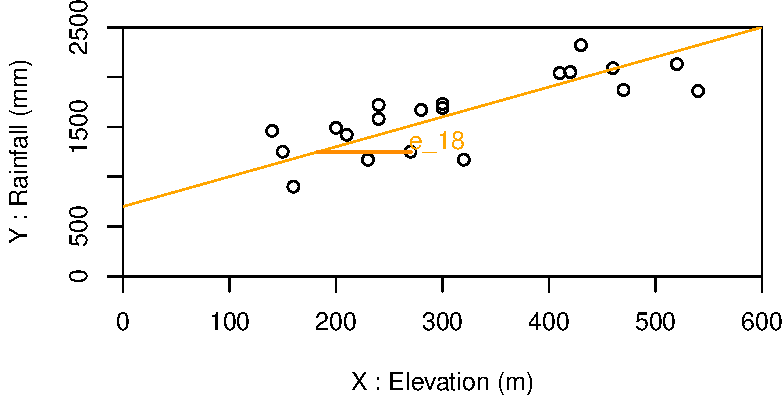
\includegraphics{072_regression_files/figure-pdf/unnamed-chunk-5-1.pdf}

As a result, \textbf{the respective role of} \(X\) and \(Y\) is not the
same in regression (compare to correlation)!!

\textbf{Regression is not symetrical}: - \(Y\) is the variable to be
explained, the \emph{dependent variable} - \(X\) is the
\emph{independent variable}

\section{Simple regression -- OLS
estimates}\label{simple-regression-ols-estimates}

How do we define the OLS line? How do we find its defining parameters
\(a\) and \(b\)?

We have the set of points \((X_i,Y_i)\), \(i=1,…,n\).

Any linear function is of the form \[Y = a + bX\], where the value for
\(a\) and \(b\) must be found.

The residual in each \(i\) is thus defined by \[e_i = Y_i - a - bX_i\]

And the OLS criteria writes as

\[\min_{a,b} = \sum_{i=1}^n e_i^2 = \sum_{i=1}^n (Y_i - a - bX_i)^2\]

Its solution is: \[a = \bar{Y}-b\bar{X}\] The intercept is completely
determined by the estimated slope \(b\) and the two sample means.

\[b = \dfrac{\sum_{i=1}^n (Y_i - \bar{Y})(X_i - \bar{X})}{\sum_{i=1}^n (X_i - \bar{X})^2} = \dfrac{\sum_{i=1}^n y_i x_i}{\sum_{i=1}^n x_i^2}\]
The denominator of \(b\) should ring a bell\ldots{} it is again the sum
of the product of the deviations to the mean in \(X\) and \(Y\), and is
thus increasing when the two changes go along in the same direction.
Conversely to the correlation coefficient, however, it is made relative
to squared changes in \(X\) not to a product of standard deviations. It
has therefore units and is expressed in units of \(Y\) per units of
\(X\) (i.e in our case \(b\) mm of precipitation for each m of
elevation)

The regression line (i.e.~estimated \(Y\)) is denoted by:
\[\hat{Y_i} = a + b X_i\] and thus the residual is
\[e_i = Y_i - \hat{Y_i}\]

In R, we use the \texttt{lm()}function to obtain \(a\) and \(b\)

\begin{Shaded}
\begin{Highlighting}[]
\FunctionTok{lm}\NormalTok{(Rainfall}\SpecialCharTok{\textasciitilde{}}\NormalTok{Elevation,}\AttributeTok{data=}\NormalTok{RainScotland)}
\CommentTok{\#\textgreater{} }
\CommentTok{\#\textgreater{} Call:}
\CommentTok{\#\textgreater{} lm(formula = Rainfall \textasciitilde{} Elevation, data = RainScotland)}
\CommentTok{\#\textgreater{} }
\CommentTok{\#\textgreater{} Coefficients:}
\CommentTok{\#\textgreater{} (Intercept)    Elevation  }
\CommentTok{\#\textgreater{}     895.322        2.377}
\end{Highlighting}
\end{Shaded}

We can store this into an object for later and to retrieve the
parameters of the line:

\begin{Shaded}
\begin{Highlighting}[]
\NormalTok{OLS1}\OtherTok{\textless{}{-}}\FunctionTok{lm}\NormalTok{(Rainfall}\SpecialCharTok{\textasciitilde{}}\NormalTok{Elevation,}\AttributeTok{data=}\NormalTok{RainScotland)}
\NormalTok{OLS1}\SpecialCharTok{$}\NormalTok{coefficients}
\CommentTok{\#\textgreater{} (Intercept)   Elevation }
\CommentTok{\#\textgreater{}  895.322341    2.377353}
\end{Highlighting}
\end{Shaded}

Where we see the best fit using the OLS estimator leads to the following
equation:
\[\hat{Y}= \text{Rainfall}  (mm) = 895 (mm) + 2.377 \text{ Elevation} (m)\]

Interpretation:

\begin{itemize}
\item
  \textbf{Every increase of 1m in elevation leads to an additional 2.377
  mm of water}
\item
  \textbf{At sea level, i.e.~elevation 0, rainfall is expected to be 895
  mm}
\item
  \textbf{If we observe an elevation of 350 m, we can expect a rainfall
  of} \(895 + 2.377 * 350= 1727 mm\)
\end{itemize}

We can represent that equation on the graph by using directly its
paramaters:

\begin{Shaded}
\begin{Highlighting}[]
\FunctionTok{plot}\NormalTok{(}\AttributeTok{x=}\NormalTok{RainScotland}\SpecialCharTok{$}\NormalTok{Elevation, }\AttributeTok{y=}\NormalTok{RainScotland}\SpecialCharTok{$}\NormalTok{Rainfall,}
    \AttributeTok{xlab=}\StringTok{"X : Elevation (m)"}\NormalTok{, }\AttributeTok{ylab=}\StringTok{"Y : Rainfall (mm)"}\NormalTok{,}
    \AttributeTok{xlim=}\FunctionTok{c}\NormalTok{(}\DecValTok{0}\NormalTok{,}\DecValTok{600}\NormalTok{), }\AttributeTok{ylim=}\FunctionTok{c}\NormalTok{(}\DecValTok{0}\NormalTok{,}\DecValTok{2500}\NormalTok{), }\AttributeTok{yaxs=}\StringTok{"i"}\NormalTok{, }\AttributeTok{xaxs=}\StringTok{"i"}\NormalTok{)}
\NormalTok{OLS\_a}\OtherTok{=}\NormalTok{OLS1}\SpecialCharTok{$}\NormalTok{coefficients[}\DecValTok{1}\NormalTok{]}
\NormalTok{OLS\_b}\OtherTok{=}\NormalTok{OLS1}\SpecialCharTok{$}\NormalTok{coefficients[}\DecValTok{2}\NormalTok{]}
\FunctionTok{abline}\NormalTok{(}\AttributeTok{a=}\NormalTok{OLS\_a,}\AttributeTok{b=}\NormalTok{OLS\_b, }\AttributeTok{col=}\StringTok{"blue"}\NormalTok{)}
\FunctionTok{text}\NormalTok{(}\AttributeTok{x=}\DecValTok{350}\NormalTok{,}\AttributeTok{y=}\DecValTok{1800}\NormalTok{,}\StringTok{"OLS"}\NormalTok{, }\AttributeTok{col=}\StringTok{"blue"}\NormalTok{)}
\end{Highlighting}
\end{Shaded}

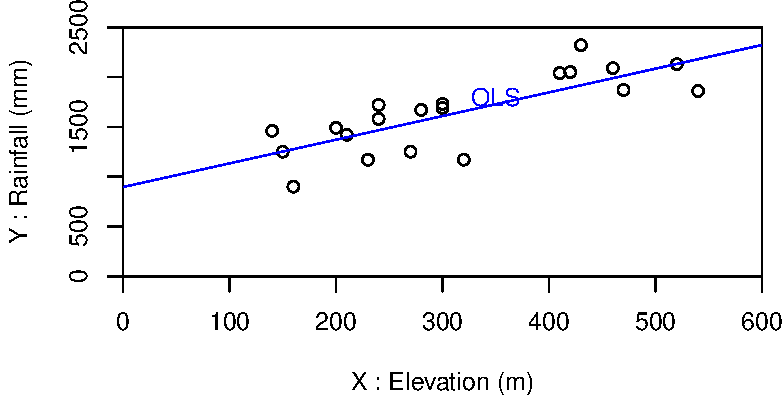
\includegraphics{072_regression_files/figure-pdf/unnamed-chunk-8-1.pdf}

\section{Quality of the
fit/prediction?}\label{quality-of-the-fitprediction}

\begin{itemize}
\item
  Use the following property: the mean prediction (estimation) equals
  the observed mean: \(\bar{Y_i} = \dfrac{1}{n} \sum_{i=1}^n \hat{Y_i}\)
\item
  Define the deviations of the estimated values to the mean:
  \(\hat{y_i} = \hat{Y_i} - \bar{Y}\)
\item
  Then the quality of the fit is
\end{itemize}

\[R^2 = \dfrac{\sum_{i=1}^n \hat{y_i^2}}{\sum_{i=1}^n y_i^2} = \dfrac{\text{Sum of squared differences to the mean that are explained}}{\text{Sum of squared differences to the mean to be explained}} = (r_{XY})^2\]
with \[0 \le R^2 \le 1\]

This R\^{}2 is displayed in the summary of the OLS model object,
together with the estimated parameters and a series of test.

\begin{Shaded}
\begin{Highlighting}[]
\FunctionTok{summary}\NormalTok{(OLS1)}
\CommentTok{\#\textgreater{} }
\CommentTok{\#\textgreater{} Call:}
\CommentTok{\#\textgreater{} lm(formula = Rainfall \textasciitilde{} Elevation, data = RainScotland)}
\CommentTok{\#\textgreater{} }
\CommentTok{\#\textgreater{} Residuals:}
\CommentTok{\#\textgreater{}     Min      1Q  Median      3Q     Max }
\CommentTok{\#\textgreater{} {-}486.08 {-}175.04   91.28  130.15  402.42 }
\CommentTok{\#\textgreater{} }
\CommentTok{\#\textgreater{} Coefficients:}
\CommentTok{\#\textgreater{}             Estimate Std. Error t value Pr(\textgreater{}|t|)    }
\CommentTok{\#\textgreater{} (Intercept) 895.3223   149.7609   5.978 1.18e{-}05 ***}
\CommentTok{\#\textgreater{} Elevation     2.3774     0.4438   5.357 4.32e{-}05 ***}
\CommentTok{\#\textgreater{} {-}{-}{-}}
\CommentTok{\#\textgreater{} Signif. codes:  0 \textquotesingle{}***\textquotesingle{} 0.001 \textquotesingle{}**\textquotesingle{} 0.01 \textquotesingle{}*\textquotesingle{} 0.05 \textquotesingle{}.\textquotesingle{} 0.1 \textquotesingle{} \textquotesingle{} 1}
\CommentTok{\#\textgreater{} }
\CommentTok{\#\textgreater{} Residual standard error: 242.8 on 18 degrees of freedom}
\CommentTok{\#\textgreater{} Multiple R{-}squared:  0.6145, Adjusted R{-}squared:  0.5931 }
\CommentTok{\#\textgreater{} F{-}statistic:  28.7 on 1 and 18 DF,  p{-}value: 4.317e{-}05}
\end{Highlighting}
\end{Shaded}

The R\^{}2 can be retreived individually from the summary itself. It is
indeed the square of the correlation coefficient:

\begin{Shaded}
\begin{Highlighting}[]
\FunctionTok{summary}\NormalTok{(OLS1)}\SpecialCharTok{$}\NormalTok{r.squared}
\CommentTok{\#\textgreater{} [1] 0.6145266}
\FunctionTok{cor}\NormalTok{(RainScotland}\SpecialCharTok{$}\NormalTok{Elevation, RainScotland}\SpecialCharTok{$}\NormalTok{Rainfall)}\SpecialCharTok{\^{}}\DecValTok{2}
\CommentTok{\#\textgreater{} [1] 0.6145266}
\end{Highlighting}
\end{Shaded}

\section{Testing:}\label{testing}

In order to know how significant are the estimated parameters and the
explained variance, we need a hypothesis related to how good the line
estimated with our sample points is to represent the true relationship
between rainfall and elevation.

This means formulating a statistical model and testing an hypothesis.

The statistical model assumes that the \(X\) values are given,
i.e.~observed with no further conditions on the distribution, and
indicate how for a given value of \(X\), we can obtain a \(Y\) value.

\subsection{True (population) line and its
estimation}\label{true-population-line-and-its-estimation}

Assume a « true » regression equation \[Y = \alpha + \beta X\]

\begin{Shaded}
\begin{Highlighting}[]
\FunctionTok{plot}\NormalTok{(}\AttributeTok{x=}\NormalTok{RainScotland}\SpecialCharTok{$}\NormalTok{Elevation, }\AttributeTok{y=}\NormalTok{RainScotland}\SpecialCharTok{$}\NormalTok{Rainfall,}
    \AttributeTok{xlab=}\StringTok{"X : Elevation (m)"}\NormalTok{, }\AttributeTok{ylab=}\StringTok{"Y : Rainfall (mm)"}\NormalTok{,}
    \AttributeTok{xlim=}\FunctionTok{c}\NormalTok{(}\DecValTok{0}\NormalTok{,}\DecValTok{600}\NormalTok{), }\AttributeTok{ylim=}\FunctionTok{c}\NormalTok{(}\DecValTok{0}\NormalTok{,}\DecValTok{2500}\NormalTok{), }\AttributeTok{yaxs=}\StringTok{"i"}\NormalTok{, }\AttributeTok{xaxs=}\StringTok{"i"}\NormalTok{)}
\NormalTok{alpha}\OtherTok{\textless{}{-}}\DecValTok{1000}
\NormalTok{beta}\OtherTok{\textless{}{-}}\DecValTok{2}
\FunctionTok{abline}\NormalTok{(}\AttributeTok{a=}\NormalTok{alpha,}\AttributeTok{b=}\NormalTok{beta, }\AttributeTok{col=}\StringTok{"goldenrod"}\NormalTok{)}
\FunctionTok{text}\NormalTok{(}\AttributeTok{x=}\DecValTok{280}\NormalTok{,}\AttributeTok{y=}\DecValTok{1900}\NormalTok{,}\FunctionTok{expression}\NormalTok{(}\FunctionTok{paste}\NormalTok{(}\StringTok{"True line "}\NormalTok{, Y }\SpecialCharTok{==}\NormalTok{ alpha }\SpecialCharTok{+}\NormalTok{ beta }\SpecialCharTok{*}\NormalTok{ X)), }\AttributeTok{col=}\StringTok{"goldenrod"}\NormalTok{)}
\end{Highlighting}
\end{Shaded}

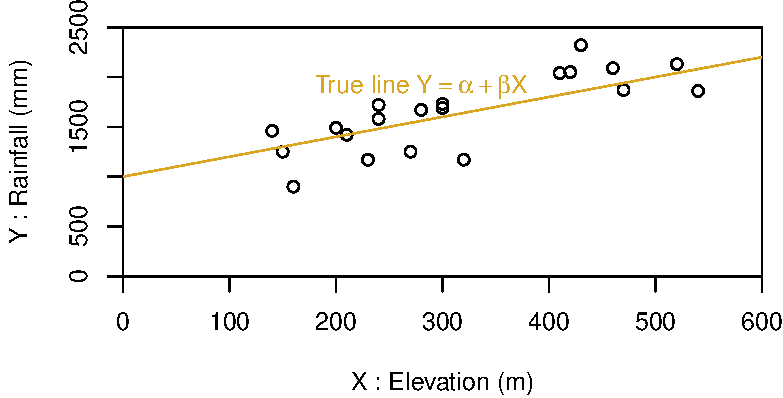
\includegraphics{072_regression_files/figure-pdf/unnamed-chunk-11-1.pdf}

Take any \(X_0\), which thus determines \(Y'_0\) from the true equation
i.e.~\(Y'_0 = \alpha + \beta X_0\). Then, add a value \(\epsilon_0\)
generated from a normal distribution \(N(0,\sigma^2)\) to \(Y’_0\) in
order to obtain \(Y_0\).

\begin{Shaded}
\begin{Highlighting}[]
\FunctionTok{set.seed}\NormalTok{(}\DecValTok{102}\NormalTok{)}
\FunctionTok{plot}\NormalTok{(}\AttributeTok{x=}\NormalTok{RainScotland}\SpecialCharTok{$}\NormalTok{Elevation, }\AttributeTok{y=}\NormalTok{RainScotland}\SpecialCharTok{$}\NormalTok{Rainfall,}
    \AttributeTok{xlab=}\StringTok{"X : Elevation (m)"}\NormalTok{, }\AttributeTok{ylab=}\StringTok{"Y : Rainfall (mm)"}\NormalTok{,}
    \AttributeTok{xlim=}\FunctionTok{c}\NormalTok{(}\DecValTok{0}\NormalTok{,}\DecValTok{600}\NormalTok{), }\AttributeTok{ylim=}\FunctionTok{c}\NormalTok{(}\DecValTok{0}\NormalTok{,}\DecValTok{2500}\NormalTok{), }\AttributeTok{yaxs=}\StringTok{"i"}\NormalTok{, }\AttributeTok{xaxs=}\StringTok{"i"}\NormalTok{)}
\NormalTok{alpha}\OtherTok{\textless{}{-}}\DecValTok{1000}
\NormalTok{beta}\OtherTok{\textless{}{-}}\DecValTok{2}
\NormalTok{epsilon}\OtherTok{\textless{}{-}}\FunctionTok{rnorm}\NormalTok{(}\AttributeTok{n=}\FunctionTok{nrow}\NormalTok{(RainScotland), }\AttributeTok{mean =} \DecValTok{0}\NormalTok{,}\AttributeTok{sd =} \DecValTok{350}\NormalTok{)}
\FunctionTok{abline}\NormalTok{(}\AttributeTok{a=}\NormalTok{alpha,}\AttributeTok{b=}\NormalTok{beta, }\AttributeTok{col=}\StringTok{"goldenrod"}\NormalTok{)}
\FunctionTok{text}\NormalTok{(}\AttributeTok{x=}\DecValTok{170}\NormalTok{,}\AttributeTok{y=}\DecValTok{2250}\NormalTok{,}\FunctionTok{expression}\NormalTok{(}\FunctionTok{paste}\NormalTok{(}\StringTok{"True line + normal errors:  "}\NormalTok{, Y[i] }\SpecialCharTok{==}\NormalTok{ alpha }\SpecialCharTok{+}\NormalTok{ beta }\SpecialCharTok{*}\NormalTok{ X[i] }\SpecialCharTok{+}\NormalTok{ epsilon[i])), }\AttributeTok{col=}\StringTok{"goldenrod"}\NormalTok{)}
\FunctionTok{points}\NormalTok{(}\AttributeTok{x=}\NormalTok{RainScotland}\SpecialCharTok{$}\NormalTok{Elevation, }\AttributeTok{y=}\NormalTok{alpha}\SpecialCharTok{+}\NormalTok{beta}\SpecialCharTok{*}\NormalTok{RainScotland}\SpecialCharTok{$}\NormalTok{Elevation}\SpecialCharTok{+}\NormalTok{epsilon, }\AttributeTok{col=}\StringTok{"goldenrod"}\NormalTok{)}
\end{Highlighting}
\end{Shaded}

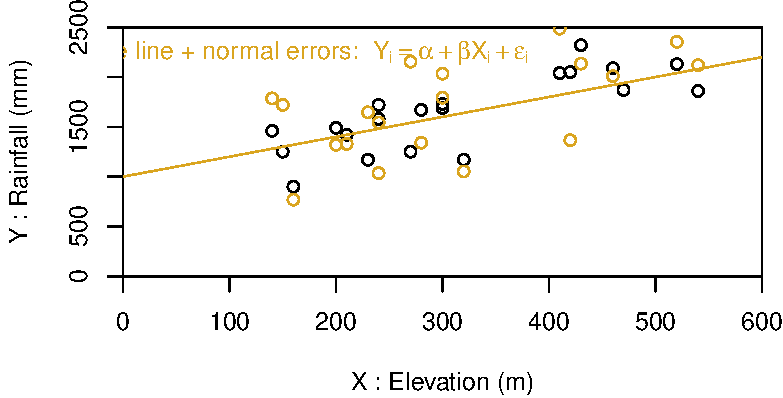
\includegraphics{072_regression_files/figure-pdf/unnamed-chunk-12-1.pdf}

Repeat for all individuals that make the population. The « true »
regression line \(Y = \alpha + \beta X\) is unknown but can be estimated
with OLS from those points. We call the \textbf{error term} \(\epsilon\)
for each point the difference between this line and the « true » line.
Conversely, to residuals \(e\), error terms \(\epsilon\) cannot be
observed. Yet we have assumed \(\epsilon\) come out of a normal
distribution around the true line and so we can formulate expectations
as to the distribution of residuals. And \(a\) et \(b\) of the OLS line
are considered as good estimators of the parameters \(\alpha\) and
\(\beta\) of the « true » regression line provided the distribution of
residuals are normal.

\begin{Shaded}
\begin{Highlighting}[]
\FunctionTok{set.seed}\NormalTok{(}\DecValTok{102}\NormalTok{)}
\FunctionTok{plot}\NormalTok{(}\AttributeTok{x=}\NormalTok{RainScotland}\SpecialCharTok{$}\NormalTok{Elevation, }\AttributeTok{y=}\NormalTok{RainScotland}\SpecialCharTok{$}\NormalTok{Rainfall,}
    \AttributeTok{xlab=}\StringTok{"X : Elevation (m)"}\NormalTok{, }\AttributeTok{ylab=}\StringTok{"Y : Rainfall (mm)"}\NormalTok{,}
    \AttributeTok{xlim=}\FunctionTok{c}\NormalTok{(}\DecValTok{0}\NormalTok{,}\DecValTok{600}\NormalTok{), }\AttributeTok{ylim=}\FunctionTok{c}\NormalTok{(}\DecValTok{0}\NormalTok{,}\DecValTok{2500}\NormalTok{), }\AttributeTok{yaxs=}\StringTok{"i"}\NormalTok{, }\AttributeTok{xaxs=}\StringTok{"i"}\NormalTok{)}
\NormalTok{alpha}\OtherTok{\textless{}{-}}\DecValTok{1000}
\NormalTok{beta}\OtherTok{\textless{}{-}}\DecValTok{2}
\NormalTok{epsilon}\OtherTok{\textless{}{-}}\FunctionTok{rnorm}\NormalTok{(}\AttributeTok{n=}\FunctionTok{nrow}\NormalTok{(RainScotland), }\AttributeTok{mean =} \DecValTok{0}\NormalTok{,}\AttributeTok{sd =} \DecValTok{350}\NormalTok{)}
\FunctionTok{abline}\NormalTok{(}\AttributeTok{a=}\NormalTok{alpha,}\AttributeTok{b=}\NormalTok{beta, }\AttributeTok{col=}\StringTok{"goldenrod"}\NormalTok{)}
\FunctionTok{text}\NormalTok{(}\AttributeTok{x=}\DecValTok{170}\NormalTok{,}\AttributeTok{y=}\DecValTok{2300}\NormalTok{,}\FunctionTok{expression}\NormalTok{(}\FunctionTok{paste}\NormalTok{(}\StringTok{"error terms:  "}\NormalTok{, epsilon[i])), }\AttributeTok{col=}\StringTok{"goldenrod"}\NormalTok{)}
\FunctionTok{text}\NormalTok{(}\AttributeTok{x=}\DecValTok{170}\NormalTok{,}\AttributeTok{y=}\DecValTok{2100}\NormalTok{,}\FunctionTok{expression}\NormalTok{(}\FunctionTok{paste}\NormalTok{(}\StringTok{"residuals:  "}\NormalTok{, e[i])), }\AttributeTok{col=}\StringTok{"blue"}\NormalTok{)}
\FunctionTok{text}\NormalTok{(}\AttributeTok{x=}\DecValTok{330}\NormalTok{,}\AttributeTok{y=}\DecValTok{1350}\NormalTok{,}\FunctionTok{expression}\NormalTok{(epsilon[i]), }\AttributeTok{col=}\StringTok{"goldenrod"}\NormalTok{)}
\FunctionTok{text}\NormalTok{(}\AttributeTok{x=}\DecValTok{310}\NormalTok{,}\AttributeTok{y=}\DecValTok{1350}\NormalTok{,}\FunctionTok{expression}\NormalTok{(e[i]), }\AttributeTok{col=}\StringTok{"blue"}\NormalTok{)}
\FunctionTok{points}\NormalTok{(}\AttributeTok{x=}\NormalTok{RainScotland}\SpecialCharTok{$}\NormalTok{Elevation, }\AttributeTok{y=}\NormalTok{alpha}\SpecialCharTok{+}\NormalTok{beta}\SpecialCharTok{*}\NormalTok{RainScotland}\SpecialCharTok{$}\NormalTok{Elevation}\SpecialCharTok{+}\NormalTok{epsilon, }\AttributeTok{col=}\StringTok{"goldenrod"}\NormalTok{)}
\FunctionTok{abline}\NormalTok{(}\AttributeTok{a=}\NormalTok{OLS\_a,}\AttributeTok{b=}\NormalTok{OLS\_b, }\AttributeTok{col=}\StringTok{"blue"}\NormalTok{)}
\FunctionTok{segments}\NormalTok{(}\AttributeTok{x0=}\NormalTok{RainScotland}\SpecialCharTok{$}\NormalTok{Elevation[}\DecValTok{19}\NormalTok{]}\SpecialCharTok{{-}}\DecValTok{2}\NormalTok{,}\AttributeTok{y0=}\NormalTok{RainScotland}\SpecialCharTok{$}\NormalTok{Rainfall[}\DecValTok{19}\NormalTok{],}
         \AttributeTok{x1=}\NormalTok{RainScotland}\SpecialCharTok{$}\NormalTok{Elevation[}\DecValTok{19}\NormalTok{]}\SpecialCharTok{{-}}\DecValTok{2}\NormalTok{, }\AttributeTok{y1=}\NormalTok{l\_a}\SpecialCharTok{+}\NormalTok{l\_b}\SpecialCharTok{*}\NormalTok{RainScotland}\SpecialCharTok{$}\NormalTok{Elevation[}\DecValTok{19}\NormalTok{], }\AttributeTok{col=}\StringTok{"blue"}\NormalTok{,}\AttributeTok{lwd=}\DecValTok{2}\NormalTok{)}
\FunctionTok{segments}\NormalTok{(}\AttributeTok{x0=}\NormalTok{RainScotland}\SpecialCharTok{$}\NormalTok{Elevation[}\DecValTok{19}\NormalTok{]}\SpecialCharTok{+}\DecValTok{2}\NormalTok{,}
         \AttributeTok{y0=}\NormalTok{alpha}\SpecialCharTok{+}\NormalTok{beta}\SpecialCharTok{*}\NormalTok{RainScotland}\SpecialCharTok{$}\NormalTok{Elevation[}\DecValTok{19}\NormalTok{]}\SpecialCharTok{+}\NormalTok{epsilon[}\DecValTok{19}\NormalTok{],}
         \AttributeTok{x1=}\NormalTok{RainScotland}\SpecialCharTok{$}\NormalTok{Elevation[}\DecValTok{19}\NormalTok{]}\SpecialCharTok{+}\DecValTok{2}\NormalTok{,}
         \AttributeTok{y1=}\NormalTok{alpha}\SpecialCharTok{+}\NormalTok{beta}\SpecialCharTok{*}\NormalTok{RainScotland}\SpecialCharTok{$}\NormalTok{Elevation[}\DecValTok{19}\NormalTok{], }\AttributeTok{col=}\StringTok{"goldenrod"}\NormalTok{,}\AttributeTok{lwd=}\DecValTok{2}\NormalTok{)}
\end{Highlighting}
\end{Shaded}

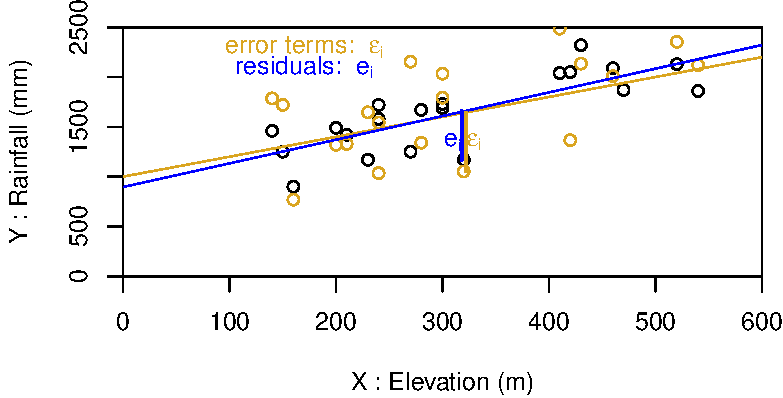
\includegraphics{072_regression_files/figure-pdf/unnamed-chunk-13-1.pdf}

\subsection{Hypotheses:}\label{hypotheses}

The null hypothesis: \(H0: Y = \alpha + \epsilon\) i.e.~assumes that
\(X\) is not useful and provides no information to find the
corresponding value of \(Y\).

The alternative hypothesis is

\(H1: Y = \alpha + \beta X + \epsilon\) i.e.~conversely, it says that
\(X\) is useful to find the right level of \(Y\).

Tests' statistics:

\begin{itemize}
\tightlist
\item
  A Student t test for each \(X\) and (intercept)
\item
  and a Fisher for the variance of the whole regression
\end{itemize}

\begin{Shaded}
\begin{Highlighting}[]
\FunctionTok{summary}\NormalTok{(OLS1)}
\CommentTok{\#\textgreater{} }
\CommentTok{\#\textgreater{} Call:}
\CommentTok{\#\textgreater{} lm(formula = Rainfall \textasciitilde{} Elevation, data = RainScotland)}
\CommentTok{\#\textgreater{} }
\CommentTok{\#\textgreater{} Residuals:}
\CommentTok{\#\textgreater{}     Min      1Q  Median      3Q     Max }
\CommentTok{\#\textgreater{} {-}486.08 {-}175.04   91.28  130.15  402.42 }
\CommentTok{\#\textgreater{} }
\CommentTok{\#\textgreater{} Coefficients:}
\CommentTok{\#\textgreater{}             Estimate Std. Error t value Pr(\textgreater{}|t|)    }
\CommentTok{\#\textgreater{} (Intercept) 895.3223   149.7609   5.978 1.18e{-}05 ***}
\CommentTok{\#\textgreater{} Elevation     2.3774     0.4438   5.357 4.32e{-}05 ***}
\CommentTok{\#\textgreater{} {-}{-}{-}}
\CommentTok{\#\textgreater{} Signif. codes:  0 \textquotesingle{}***\textquotesingle{} 0.001 \textquotesingle{}**\textquotesingle{} 0.01 \textquotesingle{}*\textquotesingle{} 0.05 \textquotesingle{}.\textquotesingle{} 0.1 \textquotesingle{} \textquotesingle{} 1}
\CommentTok{\#\textgreater{} }
\CommentTok{\#\textgreater{} Residual standard error: 242.8 on 18 degrees of freedom}
\CommentTok{\#\textgreater{} Multiple R{-}squared:  0.6145, Adjusted R{-}squared:  0.5931 }
\CommentTok{\#\textgreater{} F{-}statistic:  28.7 on 1 and 18 DF,  p{-}value: 4.317e{-}05}
\end{Highlighting}
\end{Shaded}

In our example, we see the t.tests for both our intercept and the slope
for Elevation are clearly significant. They are not zeros, we can
interpret them. And so is the F-test for the total R squared.

\section{Residuals and fitted
values:}\label{residuals-and-fitted-values}

Finally, the regression object stores - the estimated (fitted) values at
each of the individual observation - and the individual residuals, which
are terribly useful for mapping and checking that there is no other
geographical (or not) structure into play.

We can easily append both fitted values and residuals to the original
dataset:

\begin{Shaded}
\begin{Highlighting}[]
\NormalTok{RainScotland\_withmodels}\OtherTok{\textless{}{-}}\NormalTok{RainScotland}
\NormalTok{RainScotland\_withmodels}\SpecialCharTok{$}\NormalTok{fitOLS1}\OtherTok{\textless{}{-}}\NormalTok{OLS1}\SpecialCharTok{$}\NormalTok{fitted.values}
\NormalTok{RainScotland\_withmodels}\SpecialCharTok{$}\NormalTok{residOLS1}\OtherTok{\textless{}{-}}\NormalTok{OLS1}\SpecialCharTok{$}\NormalTok{residuals}
\end{Highlighting}
\end{Shaded}

\begin{Shaded}
\begin{Highlighting}[]
\FunctionTok{plot}\NormalTok{(RainScotland\_withmodels}\SpecialCharTok{$}\NormalTok{Elevation,RainScotland\_withmodels}\SpecialCharTok{$}\NormalTok{Rainfall)}
\FunctionTok{abline}\NormalTok{(}\AttributeTok{a=}\NormalTok{OLS\_a,}\AttributeTok{b=}\NormalTok{OLS\_b, }\AttributeTok{col=}\StringTok{"blue"}\NormalTok{)}
\FunctionTok{points}\NormalTok{(RainScotland\_withmodels}\SpecialCharTok{$}\NormalTok{Elevation,RainScotland\_withmodels}\SpecialCharTok{$}\NormalTok{fitOLS1, }\AttributeTok{col=}\StringTok{"blue"}\NormalTok{)}
\FunctionTok{segments}\NormalTok{(}\AttributeTok{x0=}\NormalTok{RainScotland\_withmodels}\SpecialCharTok{$}\NormalTok{Elevation,}\AttributeTok{y0=}\NormalTok{RainScotland\_withmodels}\SpecialCharTok{$}\NormalTok{Rainfall, }\AttributeTok{x=}\NormalTok{RainScotland\_withmodels}\SpecialCharTok{$}\NormalTok{Elevation,}\AttributeTok{y=}\NormalTok{RainScotland\_withmodels}\SpecialCharTok{$}\NormalTok{fitOLS1, }\AttributeTok{col=}\StringTok{"lightblue"}\NormalTok{)}
\end{Highlighting}
\end{Shaded}

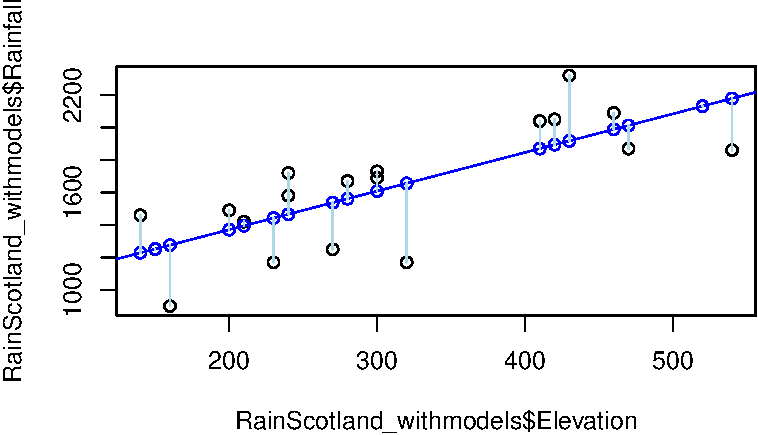
\includegraphics{072_regression_files/figure-pdf/unnamed-chunk-16-1.pdf}

One can also use the \texttt{predict()} function to estimate values at
any points, even those that were not in the sample. For example we
earlier asked what Rainfall is expected at 350m. If we have a data.frame
with \(X\) values within a column of the same name (Elevation) we can
apply the model. Suppose we want the answer for 350 and other multiples:

\begin{Shaded}
\begin{Highlighting}[]
\NormalTok{NewData}\OtherTok{\textless{}{-}}\FunctionTok{data.frame}\NormalTok{(}\AttributeTok{Elevation=}\FunctionTok{c}\NormalTok{(}\DecValTok{350}\NormalTok{,}\DecValTok{700}\NormalTok{,}\DecValTok{1050}\NormalTok{,}\DecValTok{3500}\NormalTok{))}
\FunctionTok{predict}\NormalTok{(OLS1,NewData )}
\CommentTok{\#\textgreater{}        1        2        3        4 }
\CommentTok{\#\textgreater{} 1727.396 2559.470 3391.543 9216.059}
\end{Highlighting}
\end{Shaded}

\section{Sum of residuals and the
RMSE}\label{sum-of-residuals-and-the-rmse}

The sum of the squared residuals (\emph{residualSS}, which was
minimized) can be obtained from the sum of the residuals. It is also
named the \emph{deviance} of the model.

\begin{Shaded}
\begin{Highlighting}[]
\FunctionTok{sum}\NormalTok{(}\FunctionTok{resid}\NormalTok{(OLS1)}\SpecialCharTok{\^{}}\DecValTok{2}\NormalTok{)}
\CommentTok{\#\textgreater{} [1] 1061062}
\FunctionTok{deviance}\NormalTok{(OLS1)}
\CommentTok{\#\textgreater{} [1] 1061062}
\end{Highlighting}
\end{Shaded}

\emph{residualSS} is also by definition the \emph{totalSS} minus the
\emph{explainedSS} while the \(R^2\) is the
\emph{explainedSS}/\emph{totalSS}

\begin{Shaded}
\begin{Highlighting}[]
\NormalTok{totalSS}\OtherTok{\textless{}{-}} \FunctionTok{sum}\NormalTok{((RainScotland\_withmodels}\SpecialCharTok{$}\NormalTok{Rainfall }\SpecialCharTok{{-}} \FunctionTok{mean}\NormalTok{(RainScotland\_withmodels}\SpecialCharTok{$}\NormalTok{Rainfall))}\SpecialCharTok{\^{}}\DecValTok{2}\NormalTok{)}

\NormalTok{explainedSS}\OtherTok{\textless{}{-}}\FunctionTok{sum}\NormalTok{((RainScotland\_withmodels}\SpecialCharTok{$}\NormalTok{fitOLS1 }\SpecialCharTok{{-}} \FunctionTok{mean}\NormalTok{(RainScotland\_withmodels}\SpecialCharTok{$}\NormalTok{Rainfall))}\SpecialCharTok{\^{}}\DecValTok{2}\NormalTok{)}

\NormalTok{residualSS}\OtherTok{\textless{}{-}}\NormalTok{totalSS}\SpecialCharTok{{-}}\NormalTok{explainedSS}
\NormalTok{residualSS}
\CommentTok{\#\textgreater{} [1] 1061062}
\NormalTok{R2}\OtherTok{\textless{}{-}}\NormalTok{explainedSS}\SpecialCharTok{/}\NormalTok{totalSS}
\NormalTok{R2}
\CommentTok{\#\textgreater{} [1] 0.6145266}
\end{Highlighting}
\end{Shaded}

In some fields, another metric, the Root Mean Square Error (RMSE), is
preferred over, or added to the R2 to express the performance of a
regression. The RMSE is expressed in the same units as \(Y\) and tells
us how distant on average are the predictions from the observations.

As its name indicates, the RMSE is the square root of the Mean Square
Error, which is the deviance (i.e.~residualSS) divided by the number of
observations:

\begin{Shaded}
\begin{Highlighting}[]
\NormalTok{MSE}\OtherTok{\textless{}{-}}\FunctionTok{deviance}\NormalTok{(OLS1)}\SpecialCharTok{/}\FunctionTok{nrow}\NormalTok{(RainScotland)}
\NormalTok{MSE}
\CommentTok{\#\textgreater{} [1] 53053.09}
\NormalTok{RMSE}\OtherTok{\textless{}{-}}\FunctionTok{sqrt}\NormalTok{(MSE)}
\NormalTok{RMSE}
\CommentTok{\#\textgreater{} [1] 230.3326}
\end{Highlighting}
\end{Shaded}

So we can say that on average this model of using elevation to find
rainfall levels leads to an error of around 230 mm of water per
observation.

\chapter{Confidence interval of a
regression}\label{confidence-interval-of-a-regression}

\section{Load Data and Packages}\label{load-data-and-packages}

We use the Scotland rain data and load the ggplot package plus an
additional related ggplot package (ggpmisc) to ease some formatting

\begin{Shaded}
\begin{Highlighting}[]
\NormalTok{RainScotland }\OtherTok{\textless{}{-}} \FunctionTok{read.csv}\NormalTok{(}\StringTok{"data/Ferguson/RainScotland.csv"}\NormalTok{)}
\FunctionTok{library}\NormalTok{(ggplot2)}
\FunctionTok{library}\NormalTok{(ggpmisc)}
\CommentTok{\#\textgreater{} Error in library(ggpmisc): there is no package called \textquotesingle{}ggpmisc\textquotesingle{}}
\end{Highlighting}
\end{Shaded}

\section{Scatter plot}\label{scatter-plot}

We plot the data and add the OLS line, its equation, vertical residual
lines and the confidence interval (pink area).

We emphasize two points (the 7th and 18th) for which we later calculate
the confidence interval. We see 18 is located outside of the confidence
interval and 7 is located right on the estimated line, but is also one
of the largest points in terms of elevation.

\begin{Shaded}
\begin{Highlighting}[]
\NormalTok{p}\OtherTok{\textless{}{-}}\FunctionTok{ggplot}\NormalTok{(RainScotland, }\FunctionTok{aes}\NormalTok{(}\AttributeTok{x =}\NormalTok{ Elevation, }\AttributeTok{y =}\NormalTok{ Rainfall))  }\SpecialCharTok{+}
  \FunctionTok{stat\_poly\_eq}\NormalTok{(}\FunctionTok{aes}\NormalTok{(}\AttributeTok{label =} \FunctionTok{paste}\NormalTok{(..eq.label.., ..rr.label.., }\AttributeTok{sep =} \StringTok{"\textasciitilde{}\textasciitilde{}\textasciitilde{}"}\NormalTok{)),}\AttributeTok{formula =}\NormalTok{ y }\SpecialCharTok{\textasciitilde{}}\NormalTok{ x, }\AttributeTok{parse =} \ConstantTok{TRUE}\NormalTok{) }\SpecialCharTok{+}
  \FunctionTok{geom\_smooth}\NormalTok{(}\AttributeTok{method =} \StringTok{"lm"}\NormalTok{, }\AttributeTok{se =} \ConstantTok{TRUE}\NormalTok{, }\AttributeTok{color =} \StringTok{"black"}\NormalTok{,}\AttributeTok{fill=}\StringTok{"lightpink"}\NormalTok{, }\AttributeTok{alpha =} \FloatTok{0.3}\NormalTok{)}\SpecialCharTok{+}
  \FunctionTok{geom\_segment}\NormalTok{(}\FunctionTok{aes}\NormalTok{(}\AttributeTok{xend =}\NormalTok{ Elevation, }\AttributeTok{yend =} \FunctionTok{predict}\NormalTok{(}\FunctionTok{lm}\NormalTok{(Rainfall }\SpecialCharTok{\textasciitilde{}}\NormalTok{ Elevation, }\AttributeTok{data =}\NormalTok{ RainScotland))), }\AttributeTok{linetype =} \StringTok{"dashed"}\NormalTok{, }\AttributeTok{color =} \StringTok{"gray"}\NormalTok{, }\AttributeTok{linewidth  =} \FloatTok{0.5}\NormalTok{) }\SpecialCharTok{+}
  \FunctionTok{labs}\NormalTok{(}\AttributeTok{title =} \StringTok{"Rainfall as a function of Elevation"}\NormalTok{, }\AttributeTok{x =} \StringTok{"Elevation (m)"}\NormalTok{, }\AttributeTok{y =} \StringTok{"Rainfall (mm/yr)"}\NormalTok{)}\SpecialCharTok{+}
  \FunctionTok{geom\_point}\NormalTok{(}\AttributeTok{data=}\NormalTok{RainScotland[}\DecValTok{18}\NormalTok{,], }\AttributeTok{size=}\DecValTok{5}\NormalTok{, }\AttributeTok{color=}\StringTok{"red"}\NormalTok{)}\SpecialCharTok{+}
  \FunctionTok{geom\_point}\NormalTok{(}\AttributeTok{data=}\NormalTok{RainScotland[}\DecValTok{7}\NormalTok{,], }\AttributeTok{size=}\DecValTok{5}\NormalTok{, }\AttributeTok{color=}\StringTok{"lightblue"}\NormalTok{)}\SpecialCharTok{+}
  \FunctionTok{geom\_point}\NormalTok{()}\SpecialCharTok{+}
  \FunctionTok{theme\_minimal}\NormalTok{()}
\CommentTok{\#\textgreater{} Error in stat\_poly\_eq(aes(label = paste(..eq.label.., ..rr.label.., sep = "\textasciitilde{}\textasciitilde{}\textasciitilde{}")), : could not find function "stat\_poly\_eq"}
\NormalTok{p}
\CommentTok{\#\textgreater{} Error: object \textquotesingle{}p\textquotesingle{} not found}
\end{Highlighting}
\end{Shaded}

\section{Confidence Interval
calculation}\label{confidence-interval-calculation}

We now show how the pink area representing the 95\% confidence interval
is calculated.

The lower and upper bound for each predicted value can be obtained using
the predict function. We can ask prediction and confidence bounds for
any point (using newdata with the same variables as the original
variables), but here we do it for all the observed ones and show the
values for point 7 and 18.

\begin{Shaded}
\begin{Highlighting}[]
\NormalTok{model }\OtherTok{\textless{}{-}} \FunctionTok{lm}\NormalTok{(Rainfall }\SpecialCharTok{\textasciitilde{}}\NormalTok{ Elevation, }\AttributeTok{data =}\NormalTok{ RainScotland)}

\NormalTok{pred }\OtherTok{\textless{}{-}} \FunctionTok{predict}\NormalTok{(model, }\AttributeTok{newdata =} \FunctionTok{data.frame}\NormalTok{(}\AttributeTok{Elevation =}\NormalTok{ RainScotland}\SpecialCharTok{$}\NormalTok{Elevation), }\AttributeTok{interval =} \StringTok{"confidence"}\NormalTok{)}

\NormalTok{pred[}\FunctionTok{c}\NormalTok{(}\DecValTok{7}\NormalTok{,}\DecValTok{18}\NormalTok{),]}
\CommentTok{\#\textgreater{}         fit      lwr      upr}
\CommentTok{\#\textgreater{} 7  2131.546 1908.562 2354.530}
\CommentTok{\#\textgreater{} 18 1537.208 1415.837 1658.579}

\NormalTok{predicted\_value18 }\OtherTok{\textless{}{-}}\NormalTok{ pred[}\DecValTok{18}\NormalTok{,}\StringTok{"fit"}\NormalTok{]}
\NormalTok{predicted\_value7 }\OtherTok{\textless{}{-}}\NormalTok{ pred[}\DecValTok{7}\NormalTok{,}\StringTok{"fit"}\NormalTok{]}
\end{Highlighting}
\end{Shaded}

We now compute the total \textbf{residual standard error} (RSE) of the
model (also sometimes called the Root Mean Square Error though they are
slightly different):

\[RSE=\sqrt{\frac{\sum (\text{residuals(model)})^2}{\text{model degrees of freedom}}}\]
which measures the typical distance at which the observed values fall
from the regression line. The residuals are the differences between the
observed and predicted values (our vertical dashed lines on the figure).

The sum of squared residuals is divided by the degrees of freedom. In
this case the degrees of freedom is 18 because we have n=20 individuals
and p=2 estimated parameters: the slope (2.38mm/yr) and the intercept
(elevation 895m).

(NB: I understand the denominator \(n-p\) is where RSE differs from the
Root Mean Square Error RMSE, which is often used to describe a fit,
which is the mean, i.e.~divided by \(n\))

We take the square root to get the RSE back to rainfall units, in this
case it is equal to 243mm (compare to the RMSE being 230 mm).

\begin{Shaded}
\begin{Highlighting}[]
\NormalTok{RSE}\OtherTok{\textless{}{-}}\FunctionTok{sqrt}\NormalTok{(}\FunctionTok{sum}\NormalTok{(}\FunctionTok{residuals}\NormalTok{(model)}\SpecialCharTok{\^{}}\DecValTok{2}\NormalTok{) }\SpecialCharTok{/}\NormalTok{ model}\SpecialCharTok{$}\NormalTok{df.residual)}
\NormalTok{RSE}
\CommentTok{\#\textgreater{} [1] 242.7918}
\end{Highlighting}
\end{Shaded}

Note that the RSE often denoted by sigma is also found in the summary of
the regression model:

\begin{Shaded}
\begin{Highlighting}[]
\FunctionTok{summary}\NormalTok{(model)}\SpecialCharTok{$}\NormalTok{sigma}
\CommentTok{\#\textgreater{} [1] 242.7918}
\end{Highlighting}
\end{Shaded}

For a specific observation, say the 18th or the 7th observation, we
adjust the RSE for the known characteristics of the observation,
i.e.~its value along elevation, the predictor variable. More
specifically if the observed elevation is very much away from the mean,
it is going to have a large deviation to the mean, hence a large share
of the total deviations (always squared to avoid mixing pluses and
minuses) to the mean elevation in the sample and thus potentially more
impact on the regression line.

These relative deviations are

\begin{Shaded}
\begin{Highlighting}[]
\NormalTok{elevation\_relative\_dev18}\OtherTok{\textless{}{-}}\NormalTok{(RainScotland}\SpecialCharTok{$}\NormalTok{Elevation[}\DecValTok{18}\NormalTok{] }\SpecialCharTok{{-}} \FunctionTok{mean}\NormalTok{(RainScotland}\SpecialCharTok{$}\NormalTok{Elevation))}\SpecialCharTok{\^{}}\DecValTok{2} \SpecialCharTok{/} \FunctionTok{sum}\NormalTok{((RainScotland}\SpecialCharTok{$}\NormalTok{Elevation }\SpecialCharTok{{-}} \FunctionTok{mean}\NormalTok{(RainScotland}\SpecialCharTok{$}\NormalTok{Elevation))}\SpecialCharTok{\^{}}\DecValTok{2}\NormalTok{)}

\NormalTok{elevation\_relative\_dev7}\OtherTok{\textless{}{-}}\NormalTok{(RainScotland}\SpecialCharTok{$}\NormalTok{Elevation[}\DecValTok{7}\NormalTok{] }\SpecialCharTok{{-}} \FunctionTok{mean}\NormalTok{(RainScotland}\SpecialCharTok{$}\NormalTok{Elevation))}\SpecialCharTok{\^{}}\DecValTok{2} \SpecialCharTok{/} \FunctionTok{sum}\NormalTok{((RainScotland}\SpecialCharTok{$}\NormalTok{Elevation }\SpecialCharTok{{-}} \FunctionTok{mean}\NormalTok{(RainScotland}\SpecialCharTok{$}\NormalTok{Elevation))}\SpecialCharTok{\^{}}\DecValTok{2}\NormalTok{)}

\NormalTok{elevation\_relative\_dev18}
\CommentTok{\#\textgreater{} [1] 0.006616382}
\NormalTok{elevation\_relative\_dev7}
\CommentTok{\#\textgreater{} [1] 0.1410991}
\end{Highlighting}
\end{Shaded}

Mathematically, the standard error of the fit at a given point ( \hat{y}
) is given by: \[
   \text{SE}(\hat{y}) = RSE\sqrt{\frac{1}{n} + \frac{(x - \bar{x})^2}{\sum (x_i - \bar{x})^2}}
   \]

where we see it increases with the global variance (variance of
residuals) of the model, i.e.~RSE, decreases with the sample size n, and
increases with the distance to the mean along the x variable, which is
the relative deviation quantity we just computed (compare 7 and 18).

Leaving aside the RSE, which we already calculated, we can combine the
last two terms present under the square root and define the leverage of
an observation (and simplify the standard error writing)

\[L=\frac{1}{n} + \frac{(x - \bar{x})^2}{\sum (x_i - \bar{x})^2}\\
\text{SE}(\hat{y}) = RSE\sqrt{L}\]

Leverage values range between \(\frac{1}{n}\) and 1, with higher values
indicating greater influence on the regression model. 1 is for an
observation that would stand extremely far from the mean and taking most
of the variation in x.

Points farther from the mean of x have higher leverage, have a greater
influence on the regression line and thus can increase the uncertainty
of the predicted line. In Greene (p.99) 's terms:

\begin{quote}
\emph{``the farther the forecasted point is from the center of our
experience, the greater is the degree of uncertainty''}
\end{quote}

This is why the confidence intervals (pink ribbon) usually get wider
away from the mean of x. This process is also reinforced by the density
of data points, which is typically higher around the mean of x. The
higher density providing more information and reducing uncertainty near
the mean.

The equation above also shows that the leverage will decrease for every
point as soon as n increases. When n increases the uncertainty decreases
and the ribbon is narrower.

To compute the leverage for 7 and 18 we thus simply add \(1/n\) to our
relative deviations:

\begin{Shaded}
\begin{Highlighting}[]
\NormalTok{lever7}\OtherTok{\textless{}{-}}\DecValTok{1}\SpecialCharTok{/}\FunctionTok{nrow}\NormalTok{(RainScotland)}\SpecialCharTok{+}\NormalTok{elevation\_relative\_dev7}
\NormalTok{lever18}\OtherTok{\textless{}{-}}\DecValTok{1}\SpecialCharTok{/} \FunctionTok{nrow}\NormalTok{(RainScotland)}\SpecialCharTok{+}\NormalTok{elevation\_relative\_dev18}
\NormalTok{lever7}
\CommentTok{\#\textgreater{} [1] 0.1910991}
\NormalTok{lever18}
\CommentTok{\#\textgreater{} [1] 0.05661638}
\end{Highlighting}
\end{Shaded}

With p predictors (here p=1) and n observations (here n=20), a rule of
thumb is to consider a leverage is too high when \(\frac{p+1}{n}\) is
significantly different from the average leverage. In our case, we have
\(\frac{p+1}{n}=0.1\) and observation 7 may be considered having too
much influence. In practice however, the significance of a leverage is
examined after removing high leverage points and evaluating the effect
of this removal on the regression coefficients and the overall model
fit.

Pursuing, we compute the standard errors of the fit at the level of our
observations 7 and 18:

\begin{Shaded}
\begin{Highlighting}[]
\NormalTok{se7}\OtherTok{\textless{}{-}}\NormalTok{RSE}\SpecialCharTok{*}\NormalTok{(lever7)}\SpecialCharTok{\^{}}\NormalTok{(}\DecValTok{1}\SpecialCharTok{/}\DecValTok{2}\NormalTok{)}
\NormalTok{se18}\OtherTok{\textless{}{-}}\NormalTok{RSE}\SpecialCharTok{*}\NormalTok{(lever18)}\SpecialCharTok{\^{}}\NormalTok{(}\DecValTok{1}\SpecialCharTok{/}\DecValTok{2}\NormalTok{)}
\NormalTok{se7}
\CommentTok{\#\textgreater{} [1] 106.1362}
\NormalTok{se18}
\CommentTok{\#\textgreater{} [1] 57.77037}
\end{Highlighting}
\end{Shaded}

In order to draw the pink ribbon, we need to additionally set a level of
confidence to our estimate. By default most researchers use a 95\%
confidence interval. We then multiply our point standard error by the
corresponding t-statistics, and add/remove it from the prediction to
obtain the upper and lower bounds of the confidence interval area:

We first get the critical value from the t-distribution, using half of
the 5\% (thus 0.975) on both side:

\begin{Shaded}
\begin{Highlighting}[]
\NormalTok{t\_value }\OtherTok{\textless{}{-}} \FunctionTok{qt}\NormalTok{(}\FloatTok{0.975}\NormalTok{, }\AttributeTok{df =}\NormalTok{ model}\SpecialCharTok{$}\NormalTok{df.residual)}
\end{Highlighting}
\end{Shaded}

then multiply by the standard error and add/remove it to/from
prediction:

\begin{Shaded}
\begin{Highlighting}[]
\NormalTok{lower18}\OtherTok{\textless{}{-}}\NormalTok{predicted\_value18}\SpecialCharTok{{-}}\NormalTok{t\_value}\SpecialCharTok{*}\NormalTok{se18}
\NormalTok{lower7}\OtherTok{\textless{}{-}}\NormalTok{predicted\_value7}\SpecialCharTok{{-}}\NormalTok{t\_value}\SpecialCharTok{*}\NormalTok{se7}
\NormalTok{upper18}\OtherTok{\textless{}{-}}\NormalTok{predicted\_value18}\SpecialCharTok{+}\NormalTok{t\_value}\SpecialCharTok{*}\NormalTok{se18}
\NormalTok{upper7}\OtherTok{\textless{}{-}}\NormalTok{predicted\_value7}\SpecialCharTok{+}\NormalTok{t\_value}\SpecialCharTok{*}\NormalTok{se7}

\NormalTok{manualCI}\OtherTok{\textless{}{-}}\FunctionTok{data.frame}\NormalTok{(}
  \AttributeTok{Elevation=}\NormalTok{RainScotland[}\FunctionTok{c}\NormalTok{(}\DecValTok{7}\NormalTok{,}\DecValTok{18}\NormalTok{),}\StringTok{"Elevation"}\NormalTok{],}
  \AttributeTok{UpperCI=}\FunctionTok{c}\NormalTok{(upper7,upper18),}
  \AttributeTok{LowerCI=}\FunctionTok{c}\NormalTok{(lower7,lower18)}
\NormalTok{  )}
\NormalTok{manualCI}
\CommentTok{\#\textgreater{}   Elevation  UpperCI  LowerCI}
\CommentTok{\#\textgreater{} 1       520 2354.530 1908.562}
\CommentTok{\#\textgreater{} 2       270 1658.579 1415.837}
\end{Highlighting}
\end{Shaded}

We can verify that these values are the same as the interval made up by
the predict function with the confidence option (see above)

\begin{Shaded}
\begin{Highlighting}[]
\NormalTok{pred[}\FunctionTok{c}\NormalTok{(}\DecValTok{7}\NormalTok{,}\DecValTok{18}\NormalTok{),]}
\CommentTok{\#\textgreater{}         fit      lwr      upr}
\CommentTok{\#\textgreater{} 7  2131.546 1908.562 2354.530}
\CommentTok{\#\textgreater{} 18 1537.208 1415.837 1658.579}
\end{Highlighting}
\end{Shaded}

as well as the one computed by ggplot with se=TRUE option in
geom\_smooth

\begin{Shaded}
\begin{Highlighting}[]
\NormalTok{p}\SpecialCharTok{+}\FunctionTok{geom\_segment}\NormalTok{(}\AttributeTok{data=}\NormalTok{manualCI, }\FunctionTok{aes}\NormalTok{(}\AttributeTok{x=}\NormalTok{Elevation,}\AttributeTok{xend=}\NormalTok{Elevation,}\AttributeTok{y=}\NormalTok{LowerCI, }\AttributeTok{yend =}\NormalTok{UpperCI), }\AttributeTok{color =} \StringTok{"blue"}\NormalTok{, }\AttributeTok{size =} \DecValTok{1}\NormalTok{)}
\CommentTok{\#\textgreater{} Error: object \textquotesingle{}p\textquotesingle{} not found}
\end{Highlighting}
\end{Shaded}

\section{Prediction interval versus confidence
interval}\label{prediction-interval-versus-confidence-interval}

Finally, note that there is another interval to be used for prediction
when we get new data, i.e.~the prediction interval. You can get this
interval from the predict function with the prediction option instead of
confidence.

The standard error one uses here has the same ingredients but a slightly
different definition:

\[\text{SE}(\hat{y}) = RSE\sqrt{1+ \frac{1}{n} + \frac{(x - \bar{x})^2}{\sum (x_i - \bar{x})^2}}\\
   \text{SE}(\hat{y}) = RSE\sqrt{1+L}\]

While the confidence interval we have computed previously tells you how
confident you can be that the fitted model represents well the data that
was used for estimating the model, the prediction interval is for use
when you want to infer a value for a new data based on the fitted model.

Suppose you need to infer the rainfall for a 400m elevation. You can
input the elevation (and all the other predictor variables in case of a
multiple regression) in the predict function to find the range within
which you can be 95\% confident that the new observation is included,
and thus for which the model is a reasonable tool to predict the
rainfall.

\begin{Shaded}
\begin{Highlighting}[]
\NormalTok{newdata }\OtherTok{=} \FunctionTok{data.frame}\NormalTok{(}\AttributeTok{Elevation =} \DecValTok{400}\NormalTok{)}
\NormalTok{pred\_p }\OtherTok{\textless{}{-}} \FunctionTok{predict}\NormalTok{(model, newdata, }\AttributeTok{interval =} \StringTok{"prediction"}\NormalTok{)}
\NormalTok{pred\_p}
\CommentTok{\#\textgreater{}        fit      lwr      upr}
\CommentTok{\#\textgreater{} 1 1846.264 1317.536 2374.991}
\end{Highlighting}
\end{Shaded}

In this case you can then say that there is 95\% chances that the
precipitation will be between 1318 and 2375 mm.

You can be tempted to have a more precise prediction, but you then loose
in terms of certainty.

\begin{Shaded}
\begin{Highlighting}[]
\NormalTok{pred\_p90 }\OtherTok{\textless{}{-}} \FunctionTok{predict}\NormalTok{(model, }\AttributeTok{newdata =} \FunctionTok{data.frame}\NormalTok{(}\AttributeTok{Elevation =} \DecValTok{400}\NormalTok{), }\AttributeTok{interval =} \StringTok{"prediction"}\NormalTok{, }\AttributeTok{level=}\FloatTok{0.90}\NormalTok{)}
\NormalTok{pred\_p90}
\CommentTok{\#\textgreater{}        fit      lwr      upr}
\CommentTok{\#\textgreater{} 1 1846.264 1409.861 2282.666}
\end{Highlighting}
\end{Shaded}

From 1410 to 2283 is indeed a narrower guess but it is also less
certain.

We can display the prediction area on the previous plot after taking the
values from the predict function (not directly from geom\_smooth which
logically is about the data used for estimating the curve).

\begin{Shaded}
\begin{Highlighting}[]
\NormalTok{newobs}\OtherTok{\textless{}{-}}\FunctionTok{data.frame}\NormalTok{(}\AttributeTok{Elevation =} \FunctionTok{seq}\NormalTok{(}\DecValTok{100}\NormalTok{,}\DecValTok{600}\NormalTok{, }\AttributeTok{by=}\DecValTok{50}\NormalTok{))}
\NormalTok{predictions}\OtherTok{\textless{}{-}}\FunctionTok{predict}\NormalTok{(model, }\AttributeTok{newdata =}\NormalTok{ newobs , }\AttributeTok{interval =} \StringTok{"prediction"}\NormalTok{)}
\NormalTok{p}\SpecialCharTok{+}\FunctionTok{geom\_ribbon}\NormalTok{(}\AttributeTok{data=}\FunctionTok{cbind}\NormalTok{(newobs,predictions),}\FunctionTok{aes}\NormalTok{(}\AttributeTok{x=}\NormalTok{Elevation, }\AttributeTok{y=}\ConstantTok{NULL}\NormalTok{, }\AttributeTok{ymin =}\NormalTok{ lwr, }\AttributeTok{ymax =}\NormalTok{ upr), }\AttributeTok{fill =} \StringTok{"lightblue"}\NormalTok{, }\AttributeTok{alpha =} \FloatTok{0.2}\NormalTok{)}
\CommentTok{\#\textgreater{} Error: object \textquotesingle{}p\textquotesingle{} not found}
\end{Highlighting}
\end{Shaded}

By construction, confidence intervals are narrower than prediction
intervals. Prediction intervals have an extra RSE in the calculation.
The intuition is that we don't know the mean nor the variance of the
population from which new observations are taken and the only thing we
can do is to estimate the mean from the mean of our estimates, which
itself will vary based on the variance considered. We can only use the
RSE again to estimate this variance for the mean and the variance
itself. Hence the RSE enters twice the equation.

An important implication of the presence of that extra \(1\) added to
\(L\) under the square root is that while \(L\) decreases when sample
size increases, one RSE remains and the decrease in uncertainty for the
prediction interval is limited. In other words (again Greene, p99):

\begin{quote}
``No matter how much data we have, we can never predict perfectly''
\end{quote}

\chapter{Multiple Regression}\label{multiple-regression}

Extension to use \textbf{several independent variables (regressors)}

\[Y = \alpha + \beta_1 X_1 + \beta_2 X_2 + \beta_3 X_3 ...\] \#\# Key
points:

\begin{itemize}
\item
  The model does not represent a straight line but a hyperplan.
\item
  The calculation of the quality of the fit (\(R^2\)) must be adjusted
  (particularly if lots of regressors and few observations)
\item
  The independent variables \(X_1,X_2, X_3,…\) should be
  \textbf{independent} from each other
\item
  The independent variables are not necessarily continuous ! See
  interpretation in case of factors
\end{itemize}

\section{Example with two continuous
regressors}\label{example-with-two-continuous-regressors}

Let's remind our first model with a single independent variable:

\begin{Shaded}
\begin{Highlighting}[]
\NormalTok{RainScotland}\OtherTok{\textless{}{-}}\FunctionTok{read.csv}\NormalTok{(}\StringTok{"data/Ferguson/RainScotland.csv"}\NormalTok{)}
\NormalTok{OLS1}\OtherTok{\textless{}{-}}\FunctionTok{lm}\NormalTok{(Rainfall}\SpecialCharTok{\textasciitilde{}}\NormalTok{Elevation,}\AttributeTok{data=}\NormalTok{RainScotland)}
\FunctionTok{summary}\NormalTok{(OLS1)}
\CommentTok{\#\textgreater{} }
\CommentTok{\#\textgreater{} Call:}
\CommentTok{\#\textgreater{} lm(formula = Rainfall \textasciitilde{} Elevation, data = RainScotland)}
\CommentTok{\#\textgreater{} }
\CommentTok{\#\textgreater{} Residuals:}
\CommentTok{\#\textgreater{}     Min      1Q  Median      3Q     Max }
\CommentTok{\#\textgreater{} {-}486.08 {-}175.04   91.28  130.15  402.42 }
\CommentTok{\#\textgreater{} }
\CommentTok{\#\textgreater{} Coefficients:}
\CommentTok{\#\textgreater{}             Estimate Std. Error t value Pr(\textgreater{}|t|)    }
\CommentTok{\#\textgreater{} (Intercept) 895.3223   149.7609   5.978 1.18e{-}05 ***}
\CommentTok{\#\textgreater{} Elevation     2.3774     0.4438   5.357 4.32e{-}05 ***}
\CommentTok{\#\textgreater{} {-}{-}{-}}
\CommentTok{\#\textgreater{} Signif. codes:  0 \textquotesingle{}***\textquotesingle{} 0.001 \textquotesingle{}**\textquotesingle{} 0.01 \textquotesingle{}*\textquotesingle{} 0.05 \textquotesingle{}.\textquotesingle{} 0.1 \textquotesingle{} \textquotesingle{} 1}
\CommentTok{\#\textgreater{} }
\CommentTok{\#\textgreater{} Residual standard error: 242.8 on 18 degrees of freedom}
\CommentTok{\#\textgreater{} Multiple R{-}squared:  0.6145, Adjusted R{-}squared:  0.5931 }
\CommentTok{\#\textgreater{} F{-}statistic:  28.7 on 1 and 18 DF,  p{-}value: 4.317e{-}05}
\end{Highlighting}
\end{Shaded}

We think that we can improve the model if we include the distance
(eastward) from the Western coastline and augment our model:

\begin{Shaded}
\begin{Highlighting}[]
\NormalTok{OLS2}\OtherTok{\textless{}{-}}\FunctionTok{lm}\NormalTok{(Rainfall}\SpecialCharTok{\textasciitilde{}}\NormalTok{Elevation}\SpecialCharTok{+}\NormalTok{DistanceE,}\AttributeTok{data=}\NormalTok{RainScotland)}
\FunctionTok{summary}\NormalTok{(OLS2)}
\CommentTok{\#\textgreater{} }
\CommentTok{\#\textgreater{} Call:}
\CommentTok{\#\textgreater{} lm(formula = Rainfall \textasciitilde{} Elevation + DistanceE, data = RainScotland)}
\CommentTok{\#\textgreater{} }
\CommentTok{\#\textgreater{} Residuals:}
\CommentTok{\#\textgreater{}     Min      1Q  Median      3Q     Max }
\CommentTok{\#\textgreater{} {-}268.04 {-}129.63   21.96  120.61  223.58 }
\CommentTok{\#\textgreater{} }
\CommentTok{\#\textgreater{} Coefficients:}
\CommentTok{\#\textgreater{}              Estimate Std. Error t value Pr(\textgreater{}|t|)    }
\CommentTok{\#\textgreater{} (Intercept) 1536.6951   157.6228   9.749 2.24e{-}08 ***}
\CommentTok{\#\textgreater{} Elevation      1.8238     0.3053   5.975 1.51e{-}05 ***}
\CommentTok{\#\textgreater{} DistanceE     {-}5.2209     1.0152  {-}5.143 8.14e{-}05 ***}
\CommentTok{\#\textgreater{} {-}{-}{-}}
\CommentTok{\#\textgreater{} Signif. codes:  0 \textquotesingle{}***\textquotesingle{} 0.001 \textquotesingle{}**\textquotesingle{} 0.01 \textquotesingle{}*\textquotesingle{} 0.05 \textquotesingle{}.\textquotesingle{} 0.1 \textquotesingle{} \textquotesingle{} 1}
\CommentTok{\#\textgreater{} }
\CommentTok{\#\textgreater{} Residual standard error: 156.3 on 17 degrees of freedom}
\CommentTok{\#\textgreater{} Multiple R{-}squared:  0.8492, Adjusted R{-}squared:  0.8314 }
\CommentTok{\#\textgreater{} F{-}statistic: 47.86 on 2 and 17 DF,  p{-}value: 1.04e{-}07}
\end{Highlighting}
\end{Shaded}

Compare the two models. What do you see?

First, the model is of higher quality and predictions will be better: -
More of the total variance is explained: the R-squared increased from
0.61 to 0.83 (adjusted). - the residual standard error drops from 243 to
156 mm

Second, the distance to the coast is significant and negative. It is
expressed in km, hence we interpret it as: ``when you get farther from
the Western coast, every km inland will reduce rainfall by 5.22 mm''.

Third, we could expect an interaction between elevation and distance
from the sea. We observe that introducing the distance indeed changes
our estimate of the elevation effect: from 2.38 mm of water for every m
higher, we now estimate the effect of elevation to be a 1.82 mm per m.
The effect remain well significant although it is reduced. We usually
say that this new estimate is ``\textbf{cleared from} the effect of
distance'' or ``this is the effect of elevation \textbf{after
controlling} for the effect of distance from the sea''.

\textbf{DANGER ZONE} - \textbf{DON'T COMPARE COEFFICIENTS DIRECTLY}. You
cannot say that the effect of distance is 4 times larger than the effect
of elevation! - \textbf{BEAR THE UNITS IN MIND!} \(\beta\) coefficients
have units. For example, the coefficient associated to distance is mm/km
in this case. If you had measured distance in m, the coefficient would
be -0.00522, which looks lower than the effect of elevation and much
closer to zero, but it is not!

\section{Example with one continuous and one categorical
regressor}\label{example-with-one-continuous-and-one-categorical-regressor}

Suppose you were not able to measure the distance between the
meteorological station and the sea, but you had a variable indicating
the station is in the Western part or the Eastern part of the country

Say the West variable is 1 when the collection site is on the Western
side of Scotland and 0 on the Eastern side. It is important to represent
those categorical variables as factors so their coding and effect are
not seen as a continuous one. You can also use your prefereed reference
category (here East then)

\begin{Shaded}
\begin{Highlighting}[]
\NormalTok{RainScotland}\SpecialCharTok{$}\NormalTok{West}\OtherTok{\textless{}{-}}\FunctionTok{as.factor}\NormalTok{(}\FunctionTok{as.numeric}\NormalTok{(RainScotland}\SpecialCharTok{$}\NormalTok{DistanceE}\SpecialCharTok{\textless{}}\DecValTok{90}\NormalTok{))}
\end{Highlighting}
\end{Shaded}

And we estimate a new model:

\begin{Shaded}
\begin{Highlighting}[]
\NormalTok{OLS3}\OtherTok{\textless{}{-}}\FunctionTok{lm}\NormalTok{(Rainfall}\SpecialCharTok{\textasciitilde{}}\NormalTok{Elevation}\SpecialCharTok{+}\NormalTok{West,}\AttributeTok{data=}\NormalTok{RainScotland)}
\FunctionTok{summary}\NormalTok{(OLS3)}
\CommentTok{\#\textgreater{} }
\CommentTok{\#\textgreater{} Call:}
\CommentTok{\#\textgreater{} lm(formula = Rainfall \textasciitilde{} Elevation + West, data = RainScotland)}
\CommentTok{\#\textgreater{} }
\CommentTok{\#\textgreater{} Residuals:}
\CommentTok{\#\textgreater{}      Min       1Q   Median       3Q      Max }
\CommentTok{\#\textgreater{} {-}314.920 {-}135.718   {-}1.407  103.452  309.258 }
\CommentTok{\#\textgreater{} }
\CommentTok{\#\textgreater{} Coefficients:}
\CommentTok{\#\textgreater{}             Estimate Std. Error t value Pr(\textgreater{}|t|)    }
\CommentTok{\#\textgreater{} (Intercept) 849.1774   120.4115   7.052 1.94e{-}06 ***}
\CommentTok{\#\textgreater{} Elevation     1.9867     0.3732   5.324 5.60e{-}05 ***}
\CommentTok{\#\textgreater{} West1       307.2854    91.7632   3.349  0.00381 ** }
\CommentTok{\#\textgreater{} {-}{-}{-}}
\CommentTok{\#\textgreater{} Signif. codes:  0 \textquotesingle{}***\textquotesingle{} 0.001 \textquotesingle{}**\textquotesingle{} 0.01 \textquotesingle{}*\textquotesingle{} 0.05 \textquotesingle{}.\textquotesingle{} 0.1 \textquotesingle{} \textquotesingle{} 1}
\CommentTok{\#\textgreater{} }
\CommentTok{\#\textgreater{} Residual standard error: 193.9 on 17 degrees of freedom}
\CommentTok{\#\textgreater{} Multiple R{-}squared:  0.7677, Adjusted R{-}squared:  0.7404 }
\CommentTok{\#\textgreater{} F{-}statistic:  28.1 on 2 and 17 DF,  p{-}value: 4.082e{-}06}
\end{Highlighting}
\end{Shaded}

This model 3 is less effective than model 2 in general (R-squared is
lower) but better than model 1. Also with this
\textbf{``specification''}, the elevation effect is now around 2mm.

How do you interpret the West variable coefficient? It is not continuous
so one can't phrase it as ``for every increase in\ldots{}'', rather we
will say that

\textbf{``Being in the Western part of Scotland, one can expect to add
307mm of water relative to the level of rain in the Eastern part''}

Note that now the intercept (now 849mm) refers to the level in the
Eastern part. If there were several categorical variables, it would
relate to the combined references across all variables.

Graphically you also see that introducing a categorical variable this
way leads to a fixed amount of water (307mm) to be added everywhere to
the relationship between elevation and rainfall (In some fields this is
actually called a ``fixed effect'' model):

See in red the Western point and the corresponding fit, parallel to the
corresponding fit for the Eastern stations in black.

The dashed blue line is the estimation from our first model (OLS1) for
comparison.

\begin{Shaded}
\begin{Highlighting}[]
\FunctionTok{plot}\NormalTok{(}\AttributeTok{x=}\NormalTok{RainScotland}\SpecialCharTok{$}\NormalTok{Elevation, }\AttributeTok{y=}\NormalTok{RainScotland}\SpecialCharTok{$}\NormalTok{Rainfall,}
     \AttributeTok{col=}\NormalTok{RainScotland}\SpecialCharTok{$}\NormalTok{West,}
    \AttributeTok{xlab=}\StringTok{"X : Elevation (m)"}\NormalTok{, }\AttributeTok{ylab=}\StringTok{"Y : Rainfall (mm)"}\NormalTok{)}
\FunctionTok{abline}\NormalTok{(}\AttributeTok{a=}\NormalTok{OLS3}\SpecialCharTok{$}\NormalTok{coefficients[}\DecValTok{1}\NormalTok{],}\AttributeTok{b=}\NormalTok{OLS3}\SpecialCharTok{$}\NormalTok{coefficients[}\DecValTok{2}\NormalTok{], }\AttributeTok{col=}\StringTok{"black"}\NormalTok{)}
\FunctionTok{abline}\NormalTok{(}\AttributeTok{a=}\NormalTok{OLS3}\SpecialCharTok{$}\NormalTok{coefficients[}\DecValTok{1}\NormalTok{]}\SpecialCharTok{+}\NormalTok{OLS3}\SpecialCharTok{$}\NormalTok{coefficients[}\DecValTok{3}\NormalTok{],}\AttributeTok{b=}\NormalTok{OLS3}\SpecialCharTok{$}\NormalTok{coefficients[}\DecValTok{2}\NormalTok{], }\AttributeTok{col=}\StringTok{"red"}\NormalTok{)}
\FunctionTok{abline}\NormalTok{(}\AttributeTok{a=}\NormalTok{OLS1}\SpecialCharTok{$}\NormalTok{coefficients[}\DecValTok{1}\NormalTok{],}\AttributeTok{b=}\NormalTok{OLS1}\SpecialCharTok{$}\NormalTok{coefficients[}\DecValTok{2}\NormalTok{], }\AttributeTok{col=}\StringTok{"blue"}\NormalTok{, }\AttributeTok{lty=}\DecValTok{2}\NormalTok{)}
\end{Highlighting}
\end{Shaded}

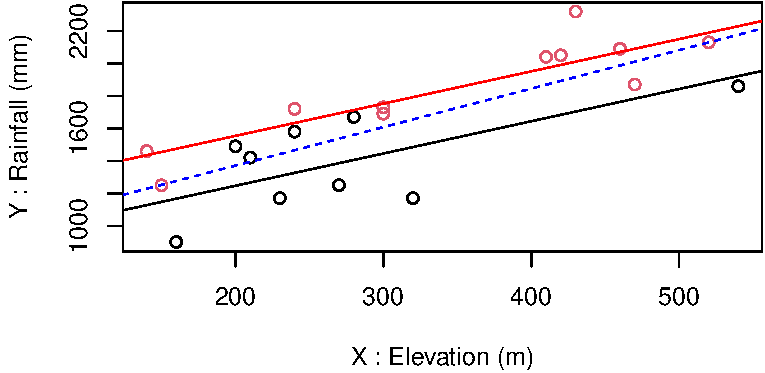
\includegraphics{074_multi_regression_files/figure-pdf/unnamed-chunk-5-1.pdf}

\section{Exercise}\label{exercise-1}

Using the dataset Lux116.csv within the data folder. - Test the
hypothesis that employment per municipality is related to `urbanness'
(using density), distance the main jobs (using road distance) and
percentage of foreigners. - Interpret the coefficients and global fit -
Test whether there could be a specific effect (downward or upward) of
being within any the 3 districts? or of belonging to Canton Luxembourg
city vs elsewhere ?

\section{Examples of multiple linear regressions from various
papers}\label{examples-of-multiple-linear-regressions-from-various-papers}

In class discussion including showing how a series of diffrent
specifications are usually presented in research papers.

\chapter{Regression diagnostics}\label{regression-diagnostics}

\section{Stressing the visual:
Anscombe}\label{stressing-the-visual-anscombe}

Consider the following 4 datasets (constructed in 1973 by the
statistician Francis Anscombe).

\begin{Shaded}
\begin{Highlighting}[]
\NormalTok{anscombe}
\CommentTok{\#\textgreater{}    x1 x2 x3 x4    y1   y2    y3    y4}
\CommentTok{\#\textgreater{} 1  10 10 10  8  8.04 9.14  7.46  6.58}
\CommentTok{\#\textgreater{} 2   8  8  8  8  6.95 8.14  6.77  5.76}
\CommentTok{\#\textgreater{} 3  13 13 13  8  7.58 8.74 12.74  7.71}
\CommentTok{\#\textgreater{} 4   9  9  9  8  8.81 8.77  7.11  8.84}
\CommentTok{\#\textgreater{} 5  11 11 11  8  8.33 9.26  7.81  8.47}
\CommentTok{\#\textgreater{} 6  14 14 14  8  9.96 8.10  8.84  7.04}
\CommentTok{\#\textgreater{} 7   6  6  6  8  7.24 6.13  6.08  5.25}
\CommentTok{\#\textgreater{} 8   4  4  4 19  4.26 3.10  5.39 12.50}
\CommentTok{\#\textgreater{} 9  12 12 12  8 10.84 9.13  8.15  5.56}
\CommentTok{\#\textgreater{} 10  7  7  7  8  4.82 7.26  6.42  7.91}
\CommentTok{\#\textgreater{} 11  5  5  5  8  5.68 4.74  5.73  6.89}
\end{Highlighting}
\end{Shaded}

In each case the mean and variance of \(Xs\) an \(Ys\) are almost
exactly the same:

\begin{Shaded}
\begin{Highlighting}[]
\FunctionTok{sapply}\NormalTok{(anscombe, mean)}
\CommentTok{\#\textgreater{}       x1       x2       x3       x4       y1       y2       y3       y4 }
\CommentTok{\#\textgreater{} 9.000000 9.000000 9.000000 9.000000 7.500909 7.500909 7.500000 7.500909}
\FunctionTok{sapply}\NormalTok{(anscombe, var)}
\CommentTok{\#\textgreater{}        x1        x2        x3        x4        y1        y2        y3        y4 }
\CommentTok{\#\textgreater{} 11.000000 11.000000 11.000000 11.000000  4.127269  4.127629  4.122620  4.123249}
\end{Highlighting}
\end{Shaded}

We estimate 4 OLS models:

\begin{Shaded}
\begin{Highlighting}[]
\CommentTok{\# code from R help}
\NormalTok{ff }\OtherTok{\textless{}{-}}\NormalTok{ y }\SpecialCharTok{\textasciitilde{}}\NormalTok{ x}
\NormalTok{mods }\OtherTok{\textless{}{-}} \FunctionTok{setNames}\NormalTok{(}\FunctionTok{as.list}\NormalTok{(}\DecValTok{1}\SpecialCharTok{:}\DecValTok{4}\NormalTok{), }\FunctionTok{paste0}\NormalTok{(}\StringTok{"lm"}\NormalTok{, }\DecValTok{1}\SpecialCharTok{:}\DecValTok{4}\NormalTok{))}
\ControlFlowTok{for}\NormalTok{ (i }\ControlFlowTok{in} \DecValTok{1}\SpecialCharTok{:}\DecValTok{4}\NormalTok{) \{}
\NormalTok{    ff[}\DecValTok{2}\SpecialCharTok{:}\DecValTok{3}\NormalTok{] }\OtherTok{\textless{}{-}} \FunctionTok{lapply}\NormalTok{(}\FunctionTok{paste0}\NormalTok{(}\FunctionTok{c}\NormalTok{(}\StringTok{"y"}\NormalTok{, }\StringTok{"x"}\NormalTok{), i), as.name)}
\NormalTok{    mods[[i]] }\OtherTok{\textless{}{-}}\NormalTok{ lmi }\OtherTok{\textless{}{-}} \FunctionTok{lm}\NormalTok{(ff, }\AttributeTok{data =}\NormalTok{ anscombe)}
    \FunctionTok{print}\NormalTok{(}\FunctionTok{summary}\NormalTok{(lmi))}
\NormalTok{\}}
\CommentTok{\#\textgreater{} }
\CommentTok{\#\textgreater{} Call:}
\CommentTok{\#\textgreater{} lm(formula = ff, data = anscombe)}
\CommentTok{\#\textgreater{} }
\CommentTok{\#\textgreater{} Residuals:}
\CommentTok{\#\textgreater{}      Min       1Q   Median       3Q      Max }
\CommentTok{\#\textgreater{} {-}1.92127 {-}0.45577 {-}0.04136  0.70941  1.83882 }
\CommentTok{\#\textgreater{} }
\CommentTok{\#\textgreater{} Coefficients:}
\CommentTok{\#\textgreater{}             Estimate Std. Error t value Pr(\textgreater{}|t|)   }
\CommentTok{\#\textgreater{} (Intercept)   3.0001     1.1247   2.667  0.02573 * }
\CommentTok{\#\textgreater{} x1            0.5001     0.1179   4.241  0.00217 **}
\CommentTok{\#\textgreater{} {-}{-}{-}}
\CommentTok{\#\textgreater{} Signif. codes:  0 \textquotesingle{}***\textquotesingle{} 0.001 \textquotesingle{}**\textquotesingle{} 0.01 \textquotesingle{}*\textquotesingle{} 0.05 \textquotesingle{}.\textquotesingle{} 0.1 \textquotesingle{} \textquotesingle{} 1}
\CommentTok{\#\textgreater{} }
\CommentTok{\#\textgreater{} Residual standard error: 1.237 on 9 degrees of freedom}
\CommentTok{\#\textgreater{} Multiple R{-}squared:  0.6665, Adjusted R{-}squared:  0.6295 }
\CommentTok{\#\textgreater{} F{-}statistic: 17.99 on 1 and 9 DF,  p{-}value: 0.00217}
\CommentTok{\#\textgreater{} }
\CommentTok{\#\textgreater{} }
\CommentTok{\#\textgreater{} Call:}
\CommentTok{\#\textgreater{} lm(formula = ff, data = anscombe)}
\CommentTok{\#\textgreater{} }
\CommentTok{\#\textgreater{} Residuals:}
\CommentTok{\#\textgreater{}     Min      1Q  Median      3Q     Max }
\CommentTok{\#\textgreater{} {-}1.9009 {-}0.7609  0.1291  0.9491  1.2691 }
\CommentTok{\#\textgreater{} }
\CommentTok{\#\textgreater{} Coefficients:}
\CommentTok{\#\textgreater{}             Estimate Std. Error t value Pr(\textgreater{}|t|)   }
\CommentTok{\#\textgreater{} (Intercept)    3.001      1.125   2.667  0.02576 * }
\CommentTok{\#\textgreater{} x2             0.500      0.118   4.239  0.00218 **}
\CommentTok{\#\textgreater{} {-}{-}{-}}
\CommentTok{\#\textgreater{} Signif. codes:  0 \textquotesingle{}***\textquotesingle{} 0.001 \textquotesingle{}**\textquotesingle{} 0.01 \textquotesingle{}*\textquotesingle{} 0.05 \textquotesingle{}.\textquotesingle{} 0.1 \textquotesingle{} \textquotesingle{} 1}
\CommentTok{\#\textgreater{} }
\CommentTok{\#\textgreater{} Residual standard error: 1.237 on 9 degrees of freedom}
\CommentTok{\#\textgreater{} Multiple R{-}squared:  0.6662, Adjusted R{-}squared:  0.6292 }
\CommentTok{\#\textgreater{} F{-}statistic: 17.97 on 1 and 9 DF,  p{-}value: 0.002179}
\CommentTok{\#\textgreater{} }
\CommentTok{\#\textgreater{} }
\CommentTok{\#\textgreater{} Call:}
\CommentTok{\#\textgreater{} lm(formula = ff, data = anscombe)}
\CommentTok{\#\textgreater{} }
\CommentTok{\#\textgreater{} Residuals:}
\CommentTok{\#\textgreater{}     Min      1Q  Median      3Q     Max }
\CommentTok{\#\textgreater{} {-}1.1586 {-}0.6146 {-}0.2303  0.1540  3.2411 }
\CommentTok{\#\textgreater{} }
\CommentTok{\#\textgreater{} Coefficients:}
\CommentTok{\#\textgreater{}             Estimate Std. Error t value Pr(\textgreater{}|t|)   }
\CommentTok{\#\textgreater{} (Intercept)   3.0025     1.1245   2.670  0.02562 * }
\CommentTok{\#\textgreater{} x3            0.4997     0.1179   4.239  0.00218 **}
\CommentTok{\#\textgreater{} {-}{-}{-}}
\CommentTok{\#\textgreater{} Signif. codes:  0 \textquotesingle{}***\textquotesingle{} 0.001 \textquotesingle{}**\textquotesingle{} 0.01 \textquotesingle{}*\textquotesingle{} 0.05 \textquotesingle{}.\textquotesingle{} 0.1 \textquotesingle{} \textquotesingle{} 1}
\CommentTok{\#\textgreater{} }
\CommentTok{\#\textgreater{} Residual standard error: 1.236 on 9 degrees of freedom}
\CommentTok{\#\textgreater{} Multiple R{-}squared:  0.6663, Adjusted R{-}squared:  0.6292 }
\CommentTok{\#\textgreater{} F{-}statistic: 17.97 on 1 and 9 DF,  p{-}value: 0.002176}
\CommentTok{\#\textgreater{} }
\CommentTok{\#\textgreater{} }
\CommentTok{\#\textgreater{} Call:}
\CommentTok{\#\textgreater{} lm(formula = ff, data = anscombe)}
\CommentTok{\#\textgreater{} }
\CommentTok{\#\textgreater{} Residuals:}
\CommentTok{\#\textgreater{}    Min     1Q Median     3Q    Max }
\CommentTok{\#\textgreater{} {-}1.751 {-}0.831  0.000  0.809  1.839 }
\CommentTok{\#\textgreater{} }
\CommentTok{\#\textgreater{} Coefficients:}
\CommentTok{\#\textgreater{}             Estimate Std. Error t value Pr(\textgreater{}|t|)   }
\CommentTok{\#\textgreater{} (Intercept)   3.0017     1.1239   2.671  0.02559 * }
\CommentTok{\#\textgreater{} x4            0.4999     0.1178   4.243  0.00216 **}
\CommentTok{\#\textgreater{} {-}{-}{-}}
\CommentTok{\#\textgreater{} Signif. codes:  0 \textquotesingle{}***\textquotesingle{} 0.001 \textquotesingle{}**\textquotesingle{} 0.01 \textquotesingle{}*\textquotesingle{} 0.05 \textquotesingle{}.\textquotesingle{} 0.1 \textquotesingle{} \textquotesingle{} 1}
\CommentTok{\#\textgreater{} }
\CommentTok{\#\textgreater{} Residual standard error: 1.236 on 9 degrees of freedom}
\CommentTok{\#\textgreater{} Multiple R{-}squared:  0.6667, Adjusted R{-}squared:  0.6297 }
\CommentTok{\#\textgreater{} F{-}statistic:    18 on 1 and 9 DF,  p{-}value: 0.002165}
\end{Highlighting}
\end{Shaded}

The quality of the fit and the regression coefficients are very similar
across the 4 cases. But looking at it more closely, you see why a visual
inspection is always needed:

\begin{Shaded}
\begin{Highlighting}[]
\CommentTok{\# code from R help}
\NormalTok{op }\OtherTok{\textless{}{-}} \FunctionTok{par}\NormalTok{(}\AttributeTok{mfrow =} \FunctionTok{c}\NormalTok{(}\DecValTok{2}\NormalTok{, }\DecValTok{2}\NormalTok{), }\AttributeTok{mar =} \FloatTok{0.1} \SpecialCharTok{+} \FunctionTok{c}\NormalTok{(}\DecValTok{4}\NormalTok{, }\DecValTok{4}\NormalTok{, }\DecValTok{1}\NormalTok{, }\DecValTok{1}\NormalTok{), }\AttributeTok{oma =} \FunctionTok{c}\NormalTok{(}\DecValTok{0}\NormalTok{, }\DecValTok{0}\NormalTok{, }\DecValTok{2}\NormalTok{, }\DecValTok{0}\NormalTok{))}
\ControlFlowTok{for}\NormalTok{ (i }\ControlFlowTok{in} \DecValTok{1}\SpecialCharTok{:}\DecValTok{4}\NormalTok{) \{}
\NormalTok{    ff[}\DecValTok{2}\SpecialCharTok{:}\DecValTok{3}\NormalTok{] }\OtherTok{\textless{}{-}} \FunctionTok{lapply}\NormalTok{(}\FunctionTok{paste0}\NormalTok{(}\FunctionTok{c}\NormalTok{(}\StringTok{"y"}\NormalTok{, }\StringTok{"x"}\NormalTok{), i), as.name)}
    \FunctionTok{plot}\NormalTok{(ff, }\AttributeTok{data =}\NormalTok{ anscombe, }\AttributeTok{col =} \StringTok{"red"}\NormalTok{, }\AttributeTok{pch =} \DecValTok{21}\NormalTok{, }\AttributeTok{bg =} \StringTok{"orange"}\NormalTok{, }\AttributeTok{cex =} \FloatTok{1.2}\NormalTok{, }
        \AttributeTok{xlim =} \FunctionTok{c}\NormalTok{(}\DecValTok{3}\NormalTok{, }\DecValTok{19}\NormalTok{), }\AttributeTok{ylim =} \FunctionTok{c}\NormalTok{(}\DecValTok{3}\NormalTok{, }\DecValTok{13}\NormalTok{))}
    \FunctionTok{abline}\NormalTok{(mods[[i]], }\AttributeTok{col =} \StringTok{"blue"}\NormalTok{)}
\NormalTok{\}}
\FunctionTok{mtext}\NormalTok{(}\StringTok{"Anscombe\textquotesingle{}s 4 Regression data sets"}\NormalTok{, }\AttributeTok{outer =} \ConstantTok{TRUE}\NormalTok{, }\AttributeTok{cex =} \FloatTok{1.5}\NormalTok{)}
\end{Highlighting}
\end{Shaded}

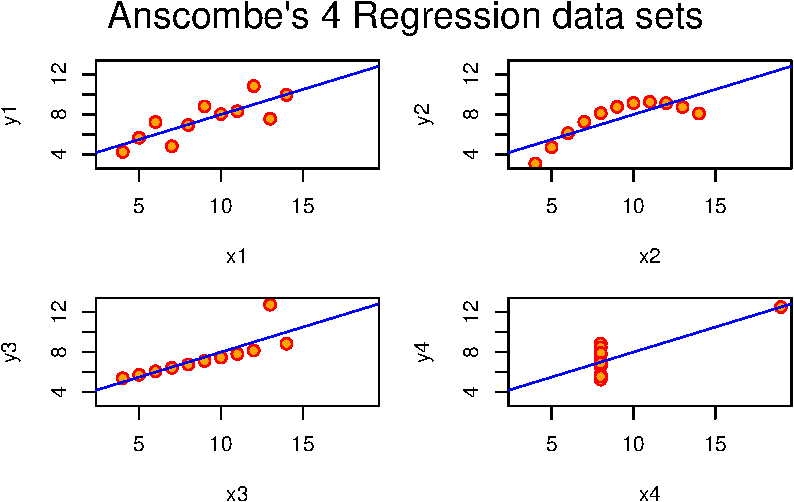
\includegraphics{075_regression_diagnostics_files/figure-pdf/unnamed-chunk-4-1.pdf}

\section{Visual diagnostics:}\label{visual-diagnostics}

\subsection{Example}\label{example-16}

\begin{Shaded}
\begin{Highlighting}[]
\NormalTok{RainScotland}\OtherTok{\textless{}{-}}\FunctionTok{read.csv}\NormalTok{(}\StringTok{"data/Ferguson/RainScotland.csv"}\NormalTok{)}
\NormalTok{OLS1}\OtherTok{\textless{}{-}}\FunctionTok{lm}\NormalTok{(Rainfall}\SpecialCharTok{\textasciitilde{}}\NormalTok{Elevation,}\AttributeTok{data=}\NormalTok{RainScotland)}
\NormalTok{OLS2}\OtherTok{\textless{}{-}}\FunctionTok{lm}\NormalTok{(Rainfall}\SpecialCharTok{\textasciitilde{}}\NormalTok{Elevation}\SpecialCharTok{+}\NormalTok{DistanceE,}\AttributeTok{data=}\NormalTok{RainScotland)}
\FunctionTok{summary}\NormalTok{(OLS2)}
\CommentTok{\#\textgreater{} }
\CommentTok{\#\textgreater{} Call:}
\CommentTok{\#\textgreater{} lm(formula = Rainfall \textasciitilde{} Elevation + DistanceE, data = RainScotland)}
\CommentTok{\#\textgreater{} }
\CommentTok{\#\textgreater{} Residuals:}
\CommentTok{\#\textgreater{}     Min      1Q  Median      3Q     Max }
\CommentTok{\#\textgreater{} {-}268.04 {-}129.63   21.96  120.61  223.58 }
\CommentTok{\#\textgreater{} }
\CommentTok{\#\textgreater{} Coefficients:}
\CommentTok{\#\textgreater{}              Estimate Std. Error t value Pr(\textgreater{}|t|)    }
\CommentTok{\#\textgreater{} (Intercept) 1536.6951   157.6228   9.749 2.24e{-}08 ***}
\CommentTok{\#\textgreater{} Elevation      1.8238     0.3053   5.975 1.51e{-}05 ***}
\CommentTok{\#\textgreater{} DistanceE     {-}5.2209     1.0152  {-}5.143 8.14e{-}05 ***}
\CommentTok{\#\textgreater{} {-}{-}{-}}
\CommentTok{\#\textgreater{} Signif. codes:  0 \textquotesingle{}***\textquotesingle{} 0.001 \textquotesingle{}**\textquotesingle{} 0.01 \textquotesingle{}*\textquotesingle{} 0.05 \textquotesingle{}.\textquotesingle{} 0.1 \textquotesingle{} \textquotesingle{} 1}
\CommentTok{\#\textgreater{} }
\CommentTok{\#\textgreater{} Residual standard error: 156.3 on 17 degrees of freedom}
\CommentTok{\#\textgreater{} Multiple R{-}squared:  0.8492, Adjusted R{-}squared:  0.8314 }
\CommentTok{\#\textgreater{} F{-}statistic: 47.86 on 2 and 17 DF,  p{-}value: 1.04e{-}07}
\end{Highlighting}
\end{Shaded}

\subsection{Plots}\label{plots}

\texttt{Plot()} applied to a \texttt{lm} object results in a sequence of
4 plots (out of 6 available) that are most useful for a visual
inspection of the relationship you uncovered, as well as assessing
whether the regression is valid and if any data behave as an outlier.

\begin{Shaded}
\begin{Highlighting}[]
\FunctionTok{par}\NormalTok{(}\AttributeTok{mfrow=}\FunctionTok{c}\NormalTok{(}\DecValTok{2}\NormalTok{,}\DecValTok{2}\NormalTok{))}
\FunctionTok{plot}\NormalTok{(OLS2)}
\end{Highlighting}
\end{Shaded}

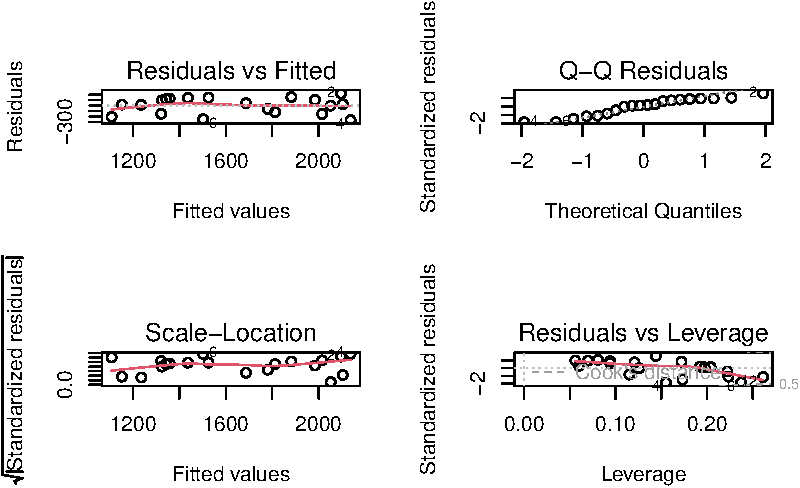
\includegraphics{075_regression_diagnostics_files/figure-pdf/unnamed-chunk-6-1.pdf}

\begin{Shaded}
\begin{Highlighting}[]
\CommentTok{\#same as}
\CommentTok{\#plot(OLS2, which=c(1,2,3,5))}
\end{Highlighting}
\end{Shaded}

\begin{itemize}
\item
  Plot 1 shows the distribution of residuals against the predicted \(Y\)
  values. For a linear relationship, one expects that the residuals are
  equally distributed along the fitted values, i.e.~spread similarly
  around the dashed horizontal line. Typically if the trend red curve
  would be clearly upward or downward sloping, or show (inverted-) U or
  V -shaped, that would mean the linearity assumption is not good. Some
  transformation or additional explanatory variables might be needed.
\item
  Plot 2 is a \texttt{qqplot} against the theoretical normal
  distribution (\texttt{qqnorm}). While we have seen that variations are
  more likely at the extremes, one expect the general shape of the curve
  to follow 1 to 1 straight line.
\item
  Plot 3 is often similar to plot 1, but more specifically aimed at
  finding if residuals are \textbf{homoscedastic}, i.e.~have equal
  variance. The residuals are standardized (studentized) and the
  smoothed red line indicates changes in the variance. Again we expect
  it to be horizontal and the points to be equally distributed within a
  horizontal rectangle buffer.
\item
  Plot 5 shows standardized residuals (same as Plot 2) now plotted
  against \texttt{leverage}, indicating whether some points may
  influence the fit more than others. Points spotted far on the right
  side of the plot may deserve some attention, as their absence may
  significantly affect the coefficients of the model. In addition,
  isolines (0.5, 1, \ldots) of Cook's distance statistic is provided.
  Again values beyond those lines must be investigated as potentially
  too influential.
\end{itemize}

Plot 4 is actually the Cook's distance alone and plot 6 another way to
represent both leverage and Cook's distance:

\begin{Shaded}
\begin{Highlighting}[]
\FunctionTok{par}\NormalTok{(}\AttributeTok{mfrow=}\FunctionTok{c}\NormalTok{(}\DecValTok{1}\NormalTok{,}\DecValTok{2}\NormalTok{))}
\FunctionTok{plot}\NormalTok{(OLS2, }\AttributeTok{which=}\FunctionTok{c}\NormalTok{(}\DecValTok{4}\NormalTok{,}\DecValTok{6}\NormalTok{))}
\end{Highlighting}
\end{Shaded}

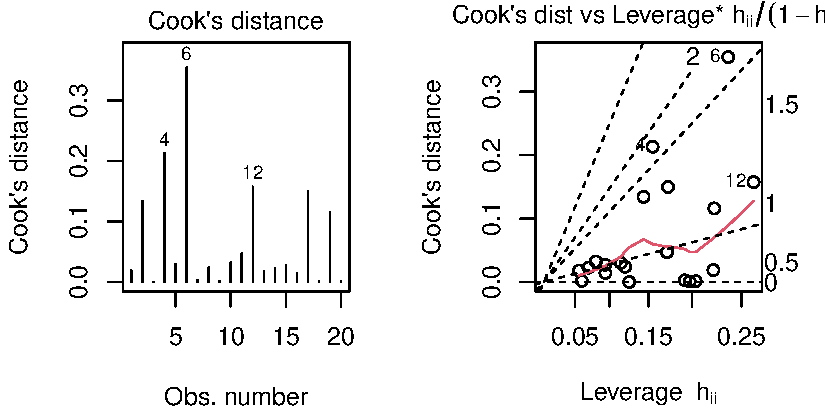
\includegraphics{075_regression_diagnostics_files/figure-pdf/unnamed-chunk-7-1.pdf}

\subsection{Plots for Anscombe data}\label{plots-for-anscombe-data}

\begin{Shaded}
\begin{Highlighting}[]
\FunctionTok{par}\NormalTok{(}\AttributeTok{mfrow=}\FunctionTok{c}\NormalTok{(}\DecValTok{2}\NormalTok{,}\DecValTok{2}\NormalTok{))}
\FunctionTok{plot}\NormalTok{(mods}\SpecialCharTok{$}\NormalTok{lm2)}
\end{Highlighting}
\end{Shaded}

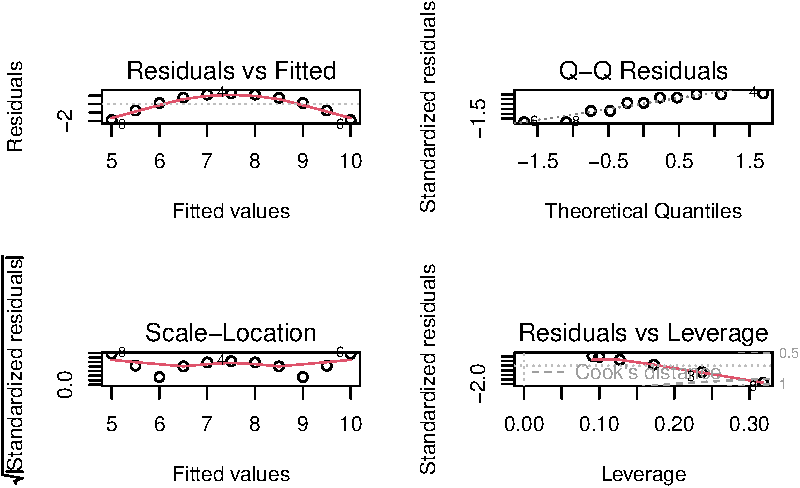
\includegraphics{075_regression_diagnostics_files/figure-pdf/unnamed-chunk-8-1.pdf}

\begin{Shaded}
\begin{Highlighting}[]
\FunctionTok{par}\NormalTok{(}\AttributeTok{mfrow=}\FunctionTok{c}\NormalTok{(}\DecValTok{2}\NormalTok{,}\DecValTok{2}\NormalTok{))}
\FunctionTok{plot}\NormalTok{(mods}\SpecialCharTok{$}\NormalTok{lm3)}
\end{Highlighting}
\end{Shaded}

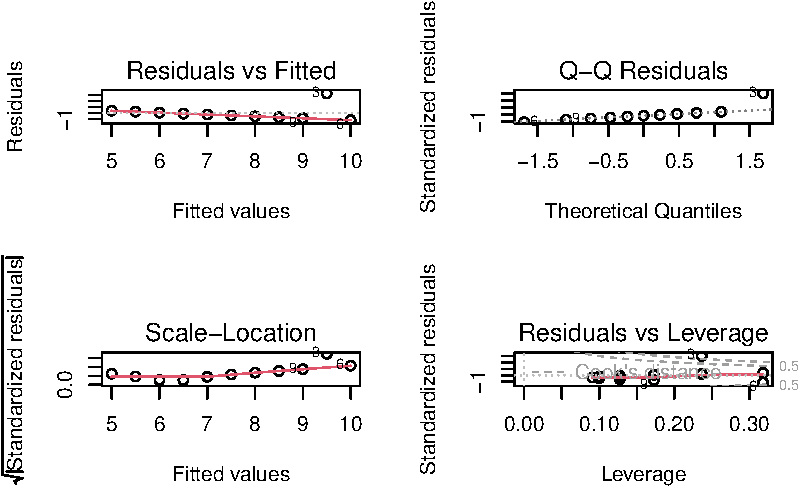
\includegraphics{075_regression_diagnostics_files/figure-pdf/unnamed-chunk-8-2.pdf}

\section{Exercise}\label{exercise-2}

Using the dataset Lux116.csv within the data folder and your previous
models, assess whether linearity and homoscedasticity are likely and
inspect the presence/effect of particulalry influencing observations

\section{Assumptions of regression
models}\label{assumptions-of-regression-models}

Deriving from Greene (table 2.1), a classical regression model relies on
a series of 6 assumptions:

\begin{enumerate}
\def\labelenumi{\arabic{enumi}.}
\item
  The model needs to specify a \textbf{linear relationship}, i.e.~a
  linear combination. Yet it doesn't mean that the elements that are
  combined (\(Y\) and or \(X\)) are not complex transforms (log, square,
  \ldots) thus leaving a lot of flexibility (semi-log,
  double-log,\ldots) to describe a relationship.
\item
  If there are several independent variables \(X\), there cannot be an
  exact linear relationship among any of them (R would tell if that is
  the case). This is the \textbf{full rank} assumption. One \(X\) cannot
  be a linear combination of some of the others.
\item
  Disturbances (error terms) in each observation are fully random draw,
  meaning that they are not a function of any of the other independent
  variables at the observation. This implies that the mean of the
  disturbances conditional to obeseving the other variables in each
  observation is zero, and subsequently that the unconditional
  \textbf{mean of disturbances is} also \textbf{zero}. See we generated
  error terms with a zero mean in the previous chapter). This
  \emph{exogeneity of the independent variables} condition is not very
  restrictive because if the mean would not be zero this could be
  captured by the intercept. It is only problematic when for some
  reasons one doesn't want an intercept (forces it to zero).
\item
  Each disturbance term has the same finite variance \emph{AND} is
  uncorrelated (independent) with every other. Having the same variance
  across observations is named \textbf{homoscedasticity} and being
  uncorrelatedness across observations is generically labelled
  \textbf{nonautocorrelation} (a special case of which is \emph{spatial
  autocorrelation} where a correlation exists due to observations being
  neighbours in space) . When verifying the two assumptions,
  disturbances are sometimes said to be \emph{spherical}.
\item
  \(X\) variables may be constants, dummy variables, or random variables
  but the process that generates them is unrelated to the process that
  generates the error terms.
\item
  It is assumed for making tests that in addition to errors having a
  zero mean (Assumption 3) and a constant variance (homoscedasticity,
  Assumption 5), that their \textbf{distribution is normal}. Following
  the Central Limit Theorem, and assumptions on how the disturbances are
  generated, the normality assumption will be reached in most cases
  where sample size is large enough. Normality is not necessary to
  obtain regression estimates but useful to several statistical tests
  (confidence intervals).
\end{enumerate}

Greene (p18), suggests the following view (see also or error terms
generation process earlier) as a summary of the assumptions, showing
that enquiring about the distribution of the residuals is key in a
regression analysis in addition to making sure the regressors are
independent.

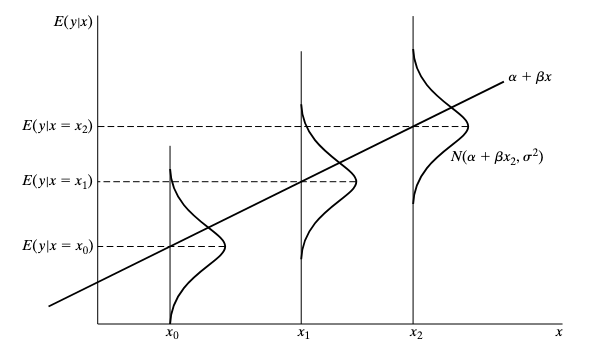
\includegraphics{images/clipboard-2284739240.png}

\section{Normality and homoscedasticity
tests}\label{normality-and-homoscedasticity-tests}

While it is not required that the dependent variable (\(Y\)) is normally
distributed, but the residuals, it is quite common to see authors
transforming their original variable to achieve a more normal
distribution before performing regression. The reason being that
residuals may deviate from normality, more easily in the case of a
non-normal \(Y\). Most important however is to verify the
homoscedasticity and normality of the residuals.

We refer to the hypothesis testing chapter for normality tests
(Shapiro-Wilk) and visualisation and focus here on the Breusch-Pagan
test of homoscedasticity, using the Scotland Rainfall models estimated
earlier.

Note that if heteroscedasticity is found, the OLS estimated coefficients
are not biased but the confidence interval we attach to them may be
wrong.

\begin{Shaded}
\begin{Highlighting}[]
\FunctionTok{summary}\NormalTok{(OLS1)}
\CommentTok{\#\textgreater{} }
\CommentTok{\#\textgreater{} Call:}
\CommentTok{\#\textgreater{} lm(formula = Rainfall \textasciitilde{} Elevation, data = RainScotland)}
\CommentTok{\#\textgreater{} }
\CommentTok{\#\textgreater{} Residuals:}
\CommentTok{\#\textgreater{}     Min      1Q  Median      3Q     Max }
\CommentTok{\#\textgreater{} {-}486.08 {-}175.04   91.28  130.15  402.42 }
\CommentTok{\#\textgreater{} }
\CommentTok{\#\textgreater{} Coefficients:}
\CommentTok{\#\textgreater{}             Estimate Std. Error t value Pr(\textgreater{}|t|)    }
\CommentTok{\#\textgreater{} (Intercept) 895.3223   149.7609   5.978 1.18e{-}05 ***}
\CommentTok{\#\textgreater{} Elevation     2.3774     0.4438   5.357 4.32e{-}05 ***}
\CommentTok{\#\textgreater{} {-}{-}{-}}
\CommentTok{\#\textgreater{} Signif. codes:  0 \textquotesingle{}***\textquotesingle{} 0.001 \textquotesingle{}**\textquotesingle{} 0.01 \textquotesingle{}*\textquotesingle{} 0.05 \textquotesingle{}.\textquotesingle{} 0.1 \textquotesingle{} \textquotesingle{} 1}
\CommentTok{\#\textgreater{} }
\CommentTok{\#\textgreater{} Residual standard error: 242.8 on 18 degrees of freedom}
\CommentTok{\#\textgreater{} Multiple R{-}squared:  0.6145, Adjusted R{-}squared:  0.5931 }
\CommentTok{\#\textgreater{} F{-}statistic:  28.7 on 1 and 18 DF,  p{-}value: 4.317e{-}05}
\FunctionTok{summary}\NormalTok{(OLS2)}
\CommentTok{\#\textgreater{} }
\CommentTok{\#\textgreater{} Call:}
\CommentTok{\#\textgreater{} lm(formula = Rainfall \textasciitilde{} Elevation + DistanceE, data = RainScotland)}
\CommentTok{\#\textgreater{} }
\CommentTok{\#\textgreater{} Residuals:}
\CommentTok{\#\textgreater{}     Min      1Q  Median      3Q     Max }
\CommentTok{\#\textgreater{} {-}268.04 {-}129.63   21.96  120.61  223.58 }
\CommentTok{\#\textgreater{} }
\CommentTok{\#\textgreater{} Coefficients:}
\CommentTok{\#\textgreater{}              Estimate Std. Error t value Pr(\textgreater{}|t|)    }
\CommentTok{\#\textgreater{} (Intercept) 1536.6951   157.6228   9.749 2.24e{-}08 ***}
\CommentTok{\#\textgreater{} Elevation      1.8238     0.3053   5.975 1.51e{-}05 ***}
\CommentTok{\#\textgreater{} DistanceE     {-}5.2209     1.0152  {-}5.143 8.14e{-}05 ***}
\CommentTok{\#\textgreater{} {-}{-}{-}}
\CommentTok{\#\textgreater{} Signif. codes:  0 \textquotesingle{}***\textquotesingle{} 0.001 \textquotesingle{}**\textquotesingle{} 0.01 \textquotesingle{}*\textquotesingle{} 0.05 \textquotesingle{}.\textquotesingle{} 0.1 \textquotesingle{} \textquotesingle{} 1}
\CommentTok{\#\textgreater{} }
\CommentTok{\#\textgreater{} Residual standard error: 156.3 on 17 degrees of freedom}
\CommentTok{\#\textgreater{} Multiple R{-}squared:  0.8492, Adjusted R{-}squared:  0.8314 }
\CommentTok{\#\textgreater{} F{-}statistic: 47.86 on 2 and 17 DF,  p{-}value: 1.04e{-}07}
\end{Highlighting}
\end{Shaded}

Starting with a histogram of the residuals:

\begin{Shaded}
\begin{Highlighting}[]
\FunctionTok{hist}\NormalTok{(}\FunctionTok{resid}\NormalTok{(OLS1))}
\end{Highlighting}
\end{Shaded}

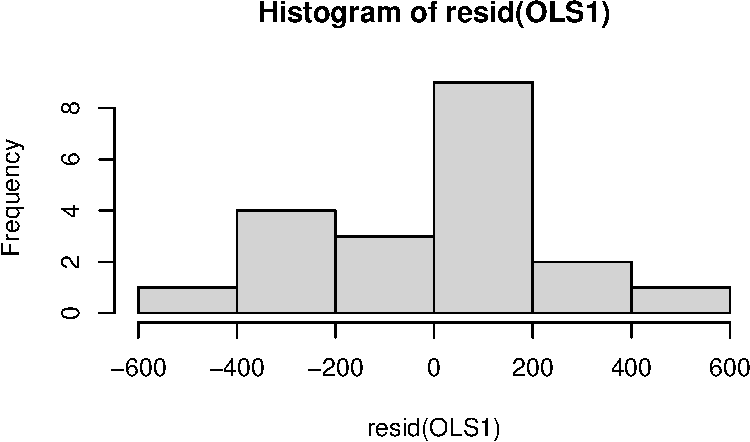
\includegraphics{075_regression_diagnostics_files/figure-pdf/unnamed-chunk-10-1.pdf}

\begin{Shaded}
\begin{Highlighting}[]
\FunctionTok{hist}\NormalTok{(}\FunctionTok{resid}\NormalTok{(OLS2))}
\end{Highlighting}
\end{Shaded}

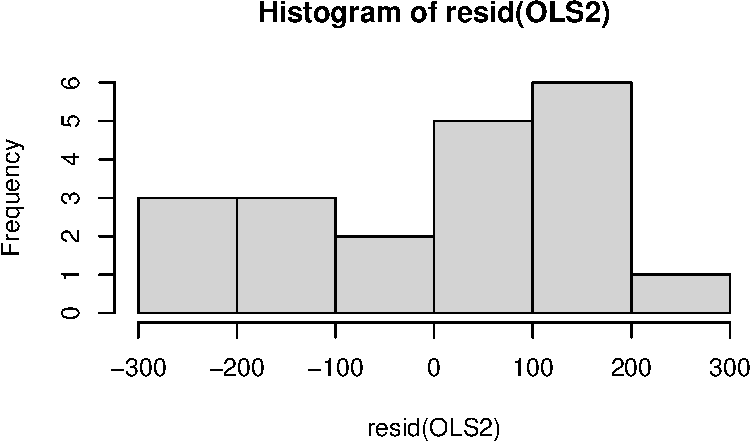
\includegraphics{075_regression_diagnostics_files/figure-pdf/unnamed-chunk-10-2.pdf}

The Breusch-Pagan test (see R help) is found within the \texttt{lmtest}
package. It fits a linear regression model to the residuals of a linear
regression model. By default the same explanatory variables are taken as
in the original regression. The null hypothesis (homoscedasticity) is
then rejected if too much of the variance (of the residuals) is
explained. The test statistic follows a chi-squared distribution with
degrees of freedom equal the number of regressors without the constant.

\begin{Shaded}
\begin{Highlighting}[]
\NormalTok{lmtest}\SpecialCharTok{::}\FunctionTok{bptest}\NormalTok{(OLS1)}
\CommentTok{\#\textgreater{} }
\CommentTok{\#\textgreater{}  studentized Breusch{-}Pagan test}
\CommentTok{\#\textgreater{} }
\CommentTok{\#\textgreater{} data:  OLS1}
\CommentTok{\#\textgreater{} BP = 0.011321, df = 1, p{-}value = 0.9153}
\NormalTok{lmtest}\SpecialCharTok{::}\FunctionTok{bptest}\NormalTok{(OLS2)}
\CommentTok{\#\textgreater{} }
\CommentTok{\#\textgreater{}  studentized Breusch{-}Pagan test}
\CommentTok{\#\textgreater{} }
\CommentTok{\#\textgreater{} data:  OLS2}
\CommentTok{\#\textgreater{} BP = 1.307, df = 2, p{-}value = 0.5202}
\end{Highlighting}
\end{Shaded}

In both cases, we can't reject the homoscedasticity, meaning our
regressions are fine on that front.

\part{Appendices, Tips, tricks and miscellaneous}

\chapter{Copy-pasting}\label{sec-copy-pasting}

\section{clipr way}\label{clipr-way}

A simple way to access to input some small data using the clipboard and
that should work across all platforms is to use the
\texttt{read\_clip()} function from the \texttt{clipr} package.

Suppose you have a series of numbers copied from a series like this one:
11 12 13 14 15 16 or this one: 11, 12, 13, 14, 15, 16

get to the console and type \texttt{clipr::read\_clip()}

In this case you will notice the whole set is a single character string
entry, which then necessitates a split. See

\begin{Shaded}
\begin{Highlighting}[]
\NormalTok{a}\OtherTok{\textless{}{-}}\NormalTok{clipr}\SpecialCharTok{::}\FunctionTok{read\_clip}\NormalTok{()}
\NormalTok{a}
\CommentTok{\#\textgreater{} [1] "11, 12, 13, 14, 15, 16"}
\FunctionTok{strsplit}\NormalTok{(a,}\StringTok{", "}\NormalTok{)}
\CommentTok{\#\textgreater{}[[1]]}
\CommentTok{\#\textgreater{}[1] "11" "12" "13" "14" "15" "16"}
\end{Highlighting}
\end{Shaded}

However, when it comes from a spreadsheet (e.g.~open office)


\includegraphics{images/clipboard-3043229473.png}

you'll get separate character entries directly:

\begin{Shaded}
\begin{Highlighting}[]
\NormalTok{clipr}\SpecialCharTok{::}\FunctionTok{read\_clip}\NormalTok{()}
\CommentTok{\#\textgreater{} [1] "0.7226332924" "0.5949296139" "0.0513909524"}
\CommentTok{\#\textgreater{} [4] "0.2215940265" "0.8725634748" "0.0032392712"}
\CommentTok{\#\textgreater{} [7] "0.774327883"  "0.1773198219" "0.1791877889"}
\CommentTok{\#\textgreater{} [10] "0.004243708"}
\end{Highlighting}
\end{Shaded}

\section{read.table way}\label{read.table-way}

You can also use the read/write table approach after saying the
clipboard in the source or output. The inconvenience is that the MacOSX
and MS Window approach have a slightly different code:

Copy from spreadsheet, then paste in R using

\begin{Shaded}
\begin{Highlighting}[]
\NormalTok{b }\OtherTok{\textless{}{-}} \FunctionTok{read.table}\NormalTok{(}\FunctionTok{pipe}\NormalTok{(}\StringTok{"pbpaste"}\NormalTok{),}\AttributeTok{header =} \ConstantTok{TRUE}\NormalTok{) }\CommentTok{\#on macOSX }
\NormalTok{b }\OtherTok{\textless{}{-}} \FunctionTok{read.table}\NormalTok{(}\StringTok{"clipboard"}\NormalTok{,}\AttributeTok{header =} \ConstantTok{TRUE}\NormalTok{) }\CommentTok{\#on MS Windows}
\end{Highlighting}
\end{Shaded}

and similarly to write to a spreadsheet:

\begin{Shaded}
\begin{Highlighting}[]
\NormalTok{b3}\OtherTok{\textless{}{-}}\NormalTok{b}\SpecialCharTok{\^{}}\DecValTok{3}
\FunctionTok{write.table}\NormalTok{(b3, }\FunctionTok{pipe}\NormalTok{(}\StringTok{"pbcopy"}\NormalTok{),}\AttributeTok{row.names =} \ConstantTok{FALSE}\NormalTok{,}\AttributeTok{sep =} \StringTok{"}\SpecialCharTok{\textbackslash{}t}\StringTok{"}\NormalTok{) }\CommentTok{\#MACOSX}
\FunctionTok{write.table}\NormalTok{(A3, }\StringTok{"clipboard"}\NormalTok{,}\AttributeTok{row.names =} \ConstantTok{FALSE}\NormalTok{,}\AttributeTok{sep =} \StringTok{"}\SpecialCharTok{\textbackslash{}t}\StringTok{"}\NormalTok{) }\CommentTok{\#MS Windows}
\end{Highlighting}
\end{Shaded}

Then paste in spreadsheet.

\chapter{Making data}\label{sec-making-data}

A number of data have been constructed from within R for the purpose of
this course.

Scripts and data can be obtained from the following course repository
within its data folder:
\url{https://github.com/geocaruso/MAGEO0641/tree/main/data}

The scripts are reproduced on this page

\section{Scraping a wikipedia table}\label{scraping-a-wikipedia-table}

Example of the Tour de France winners table from wikipedia, used in the
Vectors chapter of the course: Section~\ref{sec-factors}.

\begin{Shaded}
\begin{Highlighting}[]
\CommentTok{\#R script to scrape the tour de France winners table from wikipedia page:}
\CommentTok{\#https://en.wikipedia.org/wiki/List\_of\_Tour\_de\_France\_general\_classification\_winners}
\CommentTok{\#Geoffrey Caruso  Sept 18th 2024}
\CommentTok{\#}
\CommentTok{\# Script is adapted from}
\CommentTok{\# https://help.displayr.com/hc/en{-}us/articles/360003582875{-}How{-}to{-}Import{-}a{-}Wikipedia{-}Table{-}using{-}R}
\CommentTok{\# }
\CommentTok{\# Since there are different tables in Tour de France page and the one of interest is a sortable one,}
\CommentTok{\# I have adapted following suggestions in}
\CommentTok{\# }
\CommentTok{\# https://stackoverflow.com/questions/72380279/how{-}to{-}scrape{-}with{-}table{-}class{-}name{-}with{-}r}
\CommentTok{\# }
\CommentTok{\# I still had to look into the source of the table to find out what table class this is}
\CommentTok{\# In this case it was a "wikitable plainrowheaders sortable\textquotesingle{}}

\NormalTok{LeTour\_url}\OtherTok{\textless{}{-}}\StringTok{"https://en.wikipedia.org/wiki/List\_of\_Tour\_de\_France\_general\_classification\_winners"}
\NormalTok{LeTour\_Page}\OtherTok{\textless{}{-}}\NormalTok{rvest}\SpecialCharTok{::}\FunctionTok{read\_html}\NormalTok{(LeTour\_url)}
\NormalTok{LeTour\_Table}\OtherTok{\textless{}{-}}\NormalTok{rvest}\SpecialCharTok{::}\FunctionTok{html\_node}\NormalTok{(LeTour\_Page, }\AttributeTok{xpath=}\StringTok{"//table[@class=\textquotesingle{}wikitable plainrowheaders sortable\textquotesingle{}]"}\NormalTok{)}
\NormalTok{LeTour\_Tibble }\OtherTok{=}\NormalTok{ rvest}\SpecialCharTok{::}\FunctionTok{html\_table}\NormalTok{(LeTour\_Table, }\AttributeTok{fill =} \ConstantTok{TRUE}\NormalTok{)}
\NormalTok{LeTour\_df}\OtherTok{\textless{}{-}}\FunctionTok{as.data.frame}\NormalTok{(LeTour\_Tibble)}

\FunctionTok{saveRDS}\NormalTok{(LeTour\_df,}\StringTok{"data/TourDeFrance/LeTour\_df.rds"}\NormalTok{)}
\end{Highlighting}
\end{Shaded}

\section{Scotland rain and elevation (by
Ferguson)}\label{scotland-rain-and-elevation-by-ferguson}

\begin{Shaded}
\begin{Highlighting}[]
\CommentTok{\#Ferguson Rob,}
\CommentTok{\#linear regression in geography, CATMOG 15. https://github.com/qmrg/CATMOG/blob/Main/15{-}linear{-}regression{-}in{-}geography.pdf}

\CommentTok{\#Data from Table 1 and 2, p8:}
\CommentTok{\#Average precipitation and elevation across southern Scotland}
\CommentTok{\#}
\CommentTok{\#Source caption: British Rainfall (HMSO),}
\CommentTok{\#selected raingauges between national grid lines 600 and 601 km N.}
\CommentTok{\#Sites are in West{-}East order}
\CommentTok{\#Elevation in m above OD}
\CommentTok{\#Rainfall in mm/yr}
\CommentTok{\#DistanceE in km from W coast}
\CommentTok{\#}
\NormalTok{RainScotland}\OtherTok{\textless{}{-}}\FunctionTok{data.frame}\NormalTok{(}
  \AttributeTok{SiteNo=}\DecValTok{1}\SpecialCharTok{:}\DecValTok{20}\NormalTok{,}
  \AttributeTok{Elevation=}\FunctionTok{c}\NormalTok{(}\DecValTok{240}\NormalTok{,}\DecValTok{430}\NormalTok{,}\DecValTok{420}\NormalTok{,}\DecValTok{470}\NormalTok{,}\DecValTok{300}\NormalTok{,}\DecValTok{150}\NormalTok{,}\DecValTok{520}\NormalTok{,}\DecValTok{460}\NormalTok{,}\DecValTok{300}\NormalTok{,}\DecValTok{410}\NormalTok{,}
              \DecValTok{140}\NormalTok{,}\DecValTok{540}\NormalTok{,}\DecValTok{280}\NormalTok{,}\DecValTok{240}\NormalTok{,}\DecValTok{200}\NormalTok{,}\DecValTok{210}\NormalTok{,}\DecValTok{160}\NormalTok{,}\DecValTok{270}\NormalTok{,}\DecValTok{320}\NormalTok{,}\DecValTok{230}\NormalTok{),}
  \AttributeTok{Rainfall=}\FunctionTok{c}\NormalTok{(}\DecValTok{1720}\NormalTok{,}\DecValTok{2320}\NormalTok{,}\DecValTok{2050}\NormalTok{,}\DecValTok{1870}\NormalTok{,}\DecValTok{1690}\NormalTok{,}\DecValTok{1250}\NormalTok{,}\DecValTok{2130}\NormalTok{,}\DecValTok{2090}\NormalTok{, }\DecValTok{1730}\NormalTok{,}\DecValTok{2040}\NormalTok{,}
             \DecValTok{1460}\NormalTok{,}\DecValTok{1860}\NormalTok{,}\DecValTok{1670}\NormalTok{,}\DecValTok{1580}\NormalTok{,}\DecValTok{1490}\NormalTok{,}\DecValTok{1420}\NormalTok{,}\DecValTok{900}\NormalTok{,}\DecValTok{1250}\NormalTok{,}\DecValTok{1170}\NormalTok{,}\DecValTok{1170}\NormalTok{),}
  \AttributeTok{DistanceE=}\FunctionTok{c}\NormalTok{(}\DecValTok{37}\NormalTok{,}\DecValTok{43}\NormalTok{,}\DecValTok{48}\NormalTok{,}\DecValTok{49}\NormalTok{,}\DecValTok{52}\NormalTok{,}\DecValTok{59}\NormalTok{,}\DecValTok{73}\NormalTok{,}\DecValTok{75}\NormalTok{,}\DecValTok{76}\NormalTok{,}\DecValTok{77}\NormalTok{,}
              \DecValTok{86}\NormalTok{,}\DecValTok{97}\NormalTok{,}\DecValTok{100}\NormalTok{,}\DecValTok{103}\NormalTok{,}\DecValTok{104}\NormalTok{,}\DecValTok{114}\NormalTok{,}\DecValTok{138}\NormalTok{,}\DecValTok{152}\NormalTok{,}\DecValTok{153}\NormalTok{,}\DecValTok{154}\NormalTok{)}
\NormalTok{    )}
\FunctionTok{write.csv}\NormalTok{(RainScotland, }\StringTok{"data/Ferguson/RainScotland.csv"}\NormalTok{)}
\end{Highlighting}
\end{Shaded}

\chapter{Summary tables}\label{sec-s}

You often find yourself willing to output a summary table in a way
others can easily look at it with some visual comfort or for
publication.

This applies to descriptive statistics or the output of models.

There are no standard way of doing this in R, but many packages to do
so. I suppose a decade ago most Latex users will tend to use
\texttt{stargazer} as a way to get a tex base to be included somewhere
else. Now, especially givent the take off or markdown style reporting
and integration of notebooks and R (just like in R Studio), the choice
is more open.

Here is an example of using \texttt{summarytools} and
\texttt{modelsummary} to quickly describe an entire dataset. We invite
you to look into these packages for fine tuning, but also to be very
careful of the output. No matter how easy the outcome is to be produced
you always need to think of the relevance of any metric or graph
produced over an entire table.

\section{Descriptive statistics with
summarytools}\label{descriptive-statistics-with-summarytools}

Take the RainScotland dataset as a first example and use the
\texttt{dfSummary()} function that provides a rather comprehensive set
of statistics for entire dataframes:

\begin{Shaded}
\begin{Highlighting}[]
\NormalTok{RainScotland}\OtherTok{\textless{}{-}}\FunctionTok{read.csv}\NormalTok{(}\StringTok{"data/Ferguson/RainScotland.csv"}\NormalTok{)}
\NormalTok{summarytools}\SpecialCharTok{::}\FunctionTok{dfSummary}\NormalTok{(RainScotland)}
\CommentTok{\#\textgreater{} Error in loadNamespace(x): there is no package called \textquotesingle{}summarytools\textquotesingle{}}
\end{Highlighting}
\end{Shaded}

An nice feature is that it can generate its own view (beware:
\texttt{view} not \texttt{View()}, as an html file for display in any
browser:

\begin{Shaded}
\begin{Highlighting}[]
\NormalTok{summarytools}\SpecialCharTok{::}\FunctionTok{view}\NormalTok{(summarytools}\SpecialCharTok{::}\FunctionTok{dfSummary}\NormalTok{(RainScotland), }\AttributeTok{file =} \StringTok{"output/RainScotland.html"}\NormalTok{)}
\end{Highlighting}
\end{Shaded}


\includegraphics{images/clipboard-3105060033.png}

If we would a more complex dataset (including factors) such as the
wikipedia table of the Tour de France winners, we would have:

\begin{Shaded}
\begin{Highlighting}[]
\NormalTok{TDF}\OtherTok{\textless{}{-}}\FunctionTok{readRDS}\NormalTok{(}\StringTok{"data/TourDeFrance/LeTour\_df.rds"}\NormalTok{)}
\NormalTok{summarytools}\SpecialCharTok{::}\FunctionTok{dfSummary}\NormalTok{(TDF)}
\CommentTok{\#\textgreater{} Error in loadNamespace(x): there is no package called \textquotesingle{}summarytools\textquotesingle{}}
\end{Highlighting}
\end{Shaded}

\begin{Shaded}
\begin{Highlighting}[]
\NormalTok{summarytools}\SpecialCharTok{::}\FunctionTok{view}\NormalTok{(summarytools}\SpecialCharTok{::}\FunctionTok{dfSummary}\NormalTok{(TDF), }\AttributeTok{file =} \StringTok{"output/LeTour.html"}\NormalTok{)}
\end{Highlighting}
\end{Shaded}


\includegraphics{images/clipboard-1962764643.png}

A less visual but even more complete set (including range and indicators
of the shape of the distributions) can be obtained with the
\texttt{descr()}function.

\begin{Shaded}
\begin{Highlighting}[]
\NormalTok{summarytools}\SpecialCharTok{::}\FunctionTok{descr}\NormalTok{(RainScotland)}
\CommentTok{\#\textgreater{} Error in loadNamespace(x): there is no package called \textquotesingle{}summarytools\textquotesingle{}}
\end{Highlighting}
\end{Shaded}

In the case we apply it to the Tour de France, only the year is
available as a numeric, which is not quite interesting because there is
only one Tour per year, thus providing basically no useful information.

\begin{Shaded}
\begin{Highlighting}[]
\NormalTok{summarytools}\SpecialCharTok{::}\FunctionTok{descr}\NormalTok{(TDF)}
\CommentTok{\#\textgreater{} Error in loadNamespace(x): there is no package called \textquotesingle{}summarytools\textquotesingle{}}
\end{Highlighting}
\end{Shaded}

The specific function \texttt{freq()} is rather to be used here. Given
most variables are categorical, we are interested in counts and
percentages:

\begin{Shaded}
\begin{Highlighting}[]
\NormalTok{summarytools}\SpecialCharTok{::}\FunctionTok{freq}\NormalTok{(TDF)}
\CommentTok{\#\textgreater{} Error in loadNamespace(x): there is no package called \textquotesingle{}summarytools\textquotesingle{}}
\end{Highlighting}
\end{Shaded}

But here again we need to be careful. For example the distance variable
is coded as a character, and its reporting with frequencies is thus
quite stupid.

There is nothing automatic, you still need to think about, transform or
subset your data.

\section{Descriptive statistics with
modelsummary}\label{descriptive-statistics-with-modelsummary}

to be done

\chapter{Drawing curves in R}\label{drawing-curves-in-r}

\texttt{curve()} takes an expression, i.e.~a quote or a function call,
and evaluates it when drawing for a series of points between the from
and to limits (default 0 to 1)

\begin{Shaded}
\begin{Highlighting}[]
\FunctionTok{curve}\NormalTok{((x))}
\end{Highlighting}
\end{Shaded}

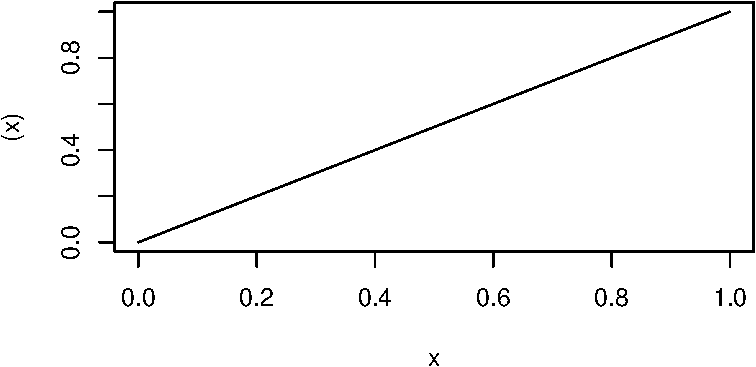
\includegraphics{904_curve_files/figure-pdf/unnamed-chunk-1-1.pdf}

\begin{Shaded}
\begin{Highlighting}[]
\FunctionTok{curve}\NormalTok{((x),}\AttributeTok{from=}\SpecialCharTok{{-}}\DecValTok{2}\NormalTok{, }\AttributeTok{to=}\DecValTok{2}\NormalTok{)}
\end{Highlighting}
\end{Shaded}

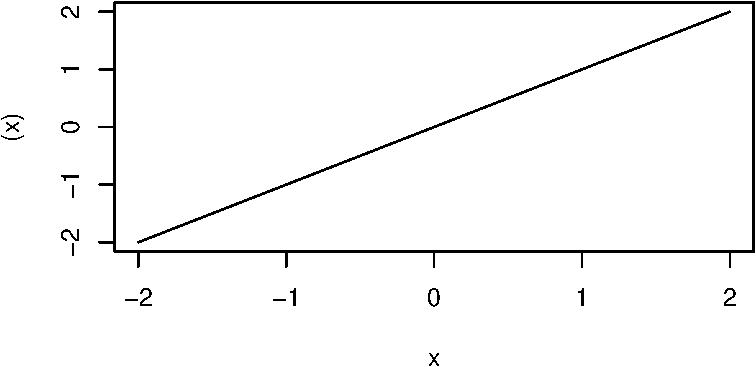
\includegraphics{904_curve_files/figure-pdf/unnamed-chunk-1-2.pdf}

\begin{Shaded}
\begin{Highlighting}[]
\FunctionTok{par}\NormalTok{(}\AttributeTok{pty=}\StringTok{"s"}\NormalTok{) }\CommentTok{\#square graphic}
\FunctionTok{curve}\NormalTok{((x),}\SpecialCharTok{{-}}\DecValTok{10}\NormalTok{,}\DecValTok{10}\NormalTok{, }\AttributeTok{axes =} \ConstantTok{FALSE}\NormalTok{, }\AttributeTok{xlim=}\FunctionTok{c}\NormalTok{(}\SpecialCharTok{{-}}\DecValTok{10}\NormalTok{,}\DecValTok{10}\NormalTok{),}\AttributeTok{ylim=}\FunctionTok{c}\NormalTok{(}\SpecialCharTok{{-}}\DecValTok{10}\NormalTok{,}\DecValTok{10}\NormalTok{))}
\FunctionTok{axis}\NormalTok{(}\DecValTok{1}\NormalTok{, }\AttributeTok{pos=}\DecValTok{0}\NormalTok{, }\AttributeTok{col=}\StringTok{"grey"}\NormalTok{)}
\FunctionTok{axis}\NormalTok{(}\DecValTok{2}\NormalTok{, }\AttributeTok{pos=}\DecValTok{0}\NormalTok{, }\AttributeTok{col=}\StringTok{"grey"}\NormalTok{)}
\FunctionTok{curve}\NormalTok{(x}\SpecialCharTok{\^{}}\DecValTok{2}\NormalTok{, }\AttributeTok{add=}\ConstantTok{TRUE}\NormalTok{, }\AttributeTok{col=}\StringTok{"blue"}\NormalTok{)}
\FunctionTok{curve}\NormalTok{(x}\SpecialCharTok{\^{}}\DecValTok{3}\NormalTok{, }\AttributeTok{add=}\ConstantTok{TRUE}\NormalTok{, }\AttributeTok{col=}\StringTok{"orange"}\NormalTok{)}
\FunctionTok{curve}\NormalTok{(log, }\AttributeTok{add=}\ConstantTok{TRUE}\NormalTok{, }\AttributeTok{col=}\StringTok{"red"}\NormalTok{)}
\CommentTok{\#\textgreater{} Warning in log(x): NaNs produced}
\FunctionTok{curve}\NormalTok{(exp, }\AttributeTok{add=}\ConstantTok{TRUE}\NormalTok{, }\AttributeTok{col=}\StringTok{"purple"}\NormalTok{)}
\end{Highlighting}
\end{Shaded}

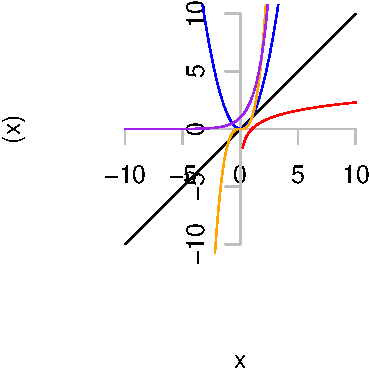
\includegraphics{904_curve_files/figure-pdf/unnamed-chunk-2-1.pdf}

\begin{Shaded}
\begin{Highlighting}[]
\FunctionTok{par}\NormalTok{(}\AttributeTok{pty=}\StringTok{"s"}\NormalTok{) }\CommentTok{\#square graphic}
\FunctionTok{curve}\NormalTok{(tan,}\SpecialCharTok{{-}}\DecValTok{5}\NormalTok{,}\DecValTok{5}\NormalTok{, }\AttributeTok{col=}\StringTok{"gold"}\NormalTok{,}
      \AttributeTok{axes =} \ConstantTok{FALSE}\NormalTok{, }\AttributeTok{xlim=}\FunctionTok{c}\NormalTok{(}\SpecialCharTok{{-}}\DecValTok{5}\NormalTok{,}\DecValTok{5}\NormalTok{),}\AttributeTok{ylim=}\FunctionTok{c}\NormalTok{(}\SpecialCharTok{{-}}\DecValTok{2}\NormalTok{,}\DecValTok{2}\NormalTok{))}
\FunctionTok{axis}\NormalTok{(}\DecValTok{1}\NormalTok{, }\AttributeTok{pos=}\DecValTok{0}\NormalTok{, }\AttributeTok{col=}\StringTok{"grey"}\NormalTok{)}
\FunctionTok{axis}\NormalTok{(}\DecValTok{2}\NormalTok{, }\AttributeTok{pos=}\DecValTok{0}\NormalTok{, }\AttributeTok{col=}\StringTok{"grey"}\NormalTok{)}
\FunctionTok{curve}\NormalTok{(cos, }\AttributeTok{add=}\ConstantTok{TRUE}\NormalTok{, }\AttributeTok{col=}\StringTok{"red"}\NormalTok{)}
\FunctionTok{curve}\NormalTok{(sin, }\AttributeTok{add=}\ConstantTok{TRUE}\NormalTok{, }\AttributeTok{col=}\StringTok{"blue"}\NormalTok{)}
\end{Highlighting}
\end{Shaded}

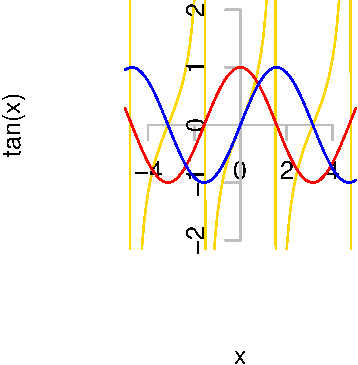
\includegraphics{904_curve_files/figure-pdf/unnamed-chunk-3-1.pdf}

\begin{Shaded}
\begin{Highlighting}[]
\FunctionTok{curve}\NormalTok{((}\FloatTok{0.3}\SpecialCharTok{*}\NormalTok{x}\SpecialCharTok{\^{}}\DecValTok{2{-}10}\SpecialCharTok{*}\NormalTok{x}\SpecialCharTok{+}\DecValTok{20}\NormalTok{), }\AttributeTok{from=}\SpecialCharTok{{-}}\DecValTok{10}\NormalTok{, }\AttributeTok{to=}\DecValTok{30}\NormalTok{)}
\end{Highlighting}
\end{Shaded}

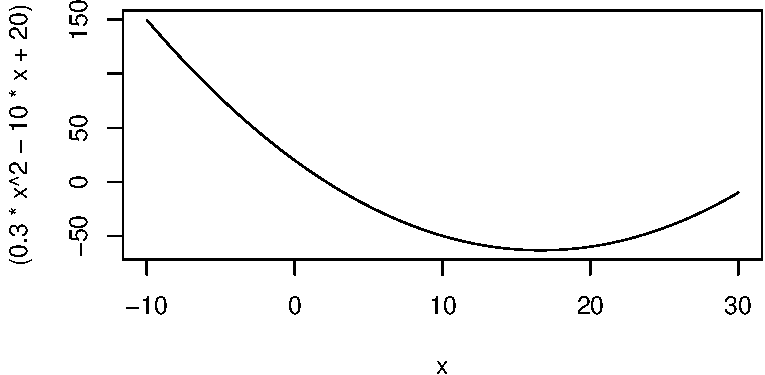
\includegraphics{904_curve_files/figure-pdf/unnamed-chunk-4-1.pdf}

\part{Bibliography}

\chapter*{References}\label{references}
\addcontentsline{toc}{chapter}{References}

\markboth{References}{References}

\phantomsection\label{refs}
\begin{CSLReferences}{1}{0}
\bibitem[\citeproctext]{ref-anselinluc1998}
Anselin, Luc, and Bera,I. 1998. {``Spatial Dependence in Linear
Regression Models with an Introduction to Spatial Econometrics:
Regression Models with an Anselin Bera i. INTRODUCTION.''} In. CRC
Press.

\bibitem[\citeproctext]{ref-beguin_axiomatic_1979}
Beguin, Hubert, and Jacques-François Thisse. 1979. {``An {Axiomatic}
{Approach} to {Geographical} {Space}.''} \emph{Geographical Analysis} 11
(4): 325--41. \url{https://doi.org/10.1111/j.1538-4632.1979.tb00700.x}.

\bibitem[\citeproctext]{ref-crawley2012}
Crawley, Michael J. 2012. \emph{The R Book}. 1st ed. Wiley.
\url{https://doi.org/10.1002/9781118448908}.

\bibitem[\citeproctext]{ref-ferguson}
Ferguson, Rob. n.d. \emph{Linear Regression in Geography}. Vol. 15.
CATMOG (Concepts And Techniques in MOdern Geography).
\url{https://github.com/qmrg/CATMOG/blob/Main/15-linear-regression-in-geography.pdf}.

\bibitem[\citeproctext]{ref-foxj2024}
Fox, J, and Weisber, S. 2024. {``An R Companion to Applied
Regression.''}
\url{https://us.sagepub.com/en-us/nam/an-r-companion-to-applied-regression/book246125}.

\bibitem[\citeproctext]{ref-haining2010}
Haining, Robert P. 2010. {``The Nature of Georeferenced Data.''} In,
edited by Manfred M. Fischer and Arthur Getis, 197--217. Berlin,
Heidelberg: Springer.
\url{https://doi.org/10.1007/978-3-642-03647-7_12}.

\bibitem[\citeproctext]{ref-long}
Long, James (JD), and Paul Teetor. n.d. \emph{R Cookbook, 2nd Edition}.
\url{https://rc2e.com/}.

\bibitem[\citeproctext]{ref-openshaw1984}
Openshaw, Stan. 1984. \emph{The Modifiable Areal Unit Problem}. Concepts
and Techniques in Modern Geography 38. Norwich: Geo.

\bibitem[\citeproctext]{ref-tobler1970}
Tobler, W. R. 1970. {``A Computer Model Simulation of Urban Growth in
the Detroit Region in Economic Geography 46: 2, 234{\textendash}240.''}
\emph{Clark University, Worcester, MA}.

\bibitem[\citeproctext]{ref-venablesbill}
Venables, Bill, and Smith, David, M. n.d. {``An Introduction to r.''}
\url{https://cran.r-project.org/doc/manuals/R-intro.html}.

\bibitem[\citeproctext]{ref-wickham}
Wickham, Hadley, Mine Çetinkaya-Rundel, and Garrett Grolemund. n.d. {``R
for Data Science (2e).''} \url{https://r4ds.hadley.nz/}.

\end{CSLReferences}




\end{document}
